% Options for packages loaded elsewhere
\PassOptionsToPackage{unicode}{hyperref}
\PassOptionsToPackage{hyphens}{url}
\PassOptionsToPackage{dvipsnames,svgnames,x11names}{xcolor}
%
\documentclass[
  letterpaper,
  DIV=11,
  numbers=noendperiod]{scrreprt}

\usepackage{amsmath,amssymb}
\usepackage{iftex}
\ifPDFTeX
  \usepackage[T1]{fontenc}
  \usepackage[utf8]{inputenc}
  \usepackage{textcomp} % provide euro and other symbols
\else % if luatex or xetex
  \usepackage{unicode-math}
  \defaultfontfeatures{Scale=MatchLowercase}
  \defaultfontfeatures[\rmfamily]{Ligatures=TeX,Scale=1}
\fi
\usepackage{lmodern}
\ifPDFTeX\else  
    % xetex/luatex font selection
\fi
% Use upquote if available, for straight quotes in verbatim environments
\IfFileExists{upquote.sty}{\usepackage{upquote}}{}
\IfFileExists{microtype.sty}{% use microtype if available
  \usepackage[]{microtype}
  \UseMicrotypeSet[protrusion]{basicmath} % disable protrusion for tt fonts
}{}
\makeatletter
\@ifundefined{KOMAClassName}{% if non-KOMA class
  \IfFileExists{parskip.sty}{%
    \usepackage{parskip}
  }{% else
    \setlength{\parindent}{0pt}
    \setlength{\parskip}{6pt plus 2pt minus 1pt}}
}{% if KOMA class
  \KOMAoptions{parskip=half}}
\makeatother
\usepackage{xcolor}
\ifLuaTeX
  \usepackage{luacolor}
  \usepackage[soul]{lua-ul}
\else
  \usepackage{soul}
  
\fi
\setlength{\emergencystretch}{3em} % prevent overfull lines
\setcounter{secnumdepth}{5}
% Make \paragraph and \subparagraph free-standing
\ifx\paragraph\undefined\else
  \let\oldparagraph\paragraph
  \renewcommand{\paragraph}[1]{\oldparagraph{#1}\mbox{}}
\fi
\ifx\subparagraph\undefined\else
  \let\oldsubparagraph\subparagraph
  \renewcommand{\subparagraph}[1]{\oldsubparagraph{#1}\mbox{}}
\fi

\usepackage{color}
\usepackage{fancyvrb}
\newcommand{\VerbBar}{|}
\newcommand{\VERB}{\Verb[commandchars=\\\{\}]}
\DefineVerbatimEnvironment{Highlighting}{Verbatim}{commandchars=\\\{\}}
% Add ',fontsize=\small' for more characters per line
\usepackage{framed}
\definecolor{shadecolor}{RGB}{241,243,245}
\newenvironment{Shaded}{\begin{snugshade}}{\end{snugshade}}
\newcommand{\AlertTok}[1]{\textcolor[rgb]{0.68,0.00,0.00}{#1}}
\newcommand{\AnnotationTok}[1]{\textcolor[rgb]{0.37,0.37,0.37}{#1}}
\newcommand{\AttributeTok}[1]{\textcolor[rgb]{0.40,0.45,0.13}{#1}}
\newcommand{\BaseNTok}[1]{\textcolor[rgb]{0.68,0.00,0.00}{#1}}
\newcommand{\BuiltInTok}[1]{\textcolor[rgb]{0.00,0.23,0.31}{#1}}
\newcommand{\CharTok}[1]{\textcolor[rgb]{0.13,0.47,0.30}{#1}}
\newcommand{\CommentTok}[1]{\textcolor[rgb]{0.37,0.37,0.37}{#1}}
\newcommand{\CommentVarTok}[1]{\textcolor[rgb]{0.37,0.37,0.37}{\textit{#1}}}
\newcommand{\ConstantTok}[1]{\textcolor[rgb]{0.56,0.35,0.01}{#1}}
\newcommand{\ControlFlowTok}[1]{\textcolor[rgb]{0.00,0.23,0.31}{#1}}
\newcommand{\DataTypeTok}[1]{\textcolor[rgb]{0.68,0.00,0.00}{#1}}
\newcommand{\DecValTok}[1]{\textcolor[rgb]{0.68,0.00,0.00}{#1}}
\newcommand{\DocumentationTok}[1]{\textcolor[rgb]{0.37,0.37,0.37}{\textit{#1}}}
\newcommand{\ErrorTok}[1]{\textcolor[rgb]{0.68,0.00,0.00}{#1}}
\newcommand{\ExtensionTok}[1]{\textcolor[rgb]{0.00,0.23,0.31}{#1}}
\newcommand{\FloatTok}[1]{\textcolor[rgb]{0.68,0.00,0.00}{#1}}
\newcommand{\FunctionTok}[1]{\textcolor[rgb]{0.28,0.35,0.67}{#1}}
\newcommand{\ImportTok}[1]{\textcolor[rgb]{0.00,0.46,0.62}{#1}}
\newcommand{\InformationTok}[1]{\textcolor[rgb]{0.37,0.37,0.37}{#1}}
\newcommand{\KeywordTok}[1]{\textcolor[rgb]{0.00,0.23,0.31}{#1}}
\newcommand{\NormalTok}[1]{\textcolor[rgb]{0.00,0.23,0.31}{#1}}
\newcommand{\OperatorTok}[1]{\textcolor[rgb]{0.37,0.37,0.37}{#1}}
\newcommand{\OtherTok}[1]{\textcolor[rgb]{0.00,0.23,0.31}{#1}}
\newcommand{\PreprocessorTok}[1]{\textcolor[rgb]{0.68,0.00,0.00}{#1}}
\newcommand{\RegionMarkerTok}[1]{\textcolor[rgb]{0.00,0.23,0.31}{#1}}
\newcommand{\SpecialCharTok}[1]{\textcolor[rgb]{0.37,0.37,0.37}{#1}}
\newcommand{\SpecialStringTok}[1]{\textcolor[rgb]{0.13,0.47,0.30}{#1}}
\newcommand{\StringTok}[1]{\textcolor[rgb]{0.13,0.47,0.30}{#1}}
\newcommand{\VariableTok}[1]{\textcolor[rgb]{0.07,0.07,0.07}{#1}}
\newcommand{\VerbatimStringTok}[1]{\textcolor[rgb]{0.13,0.47,0.30}{#1}}
\newcommand{\WarningTok}[1]{\textcolor[rgb]{0.37,0.37,0.37}{\textit{#1}}}

\providecommand{\tightlist}{%
  \setlength{\itemsep}{0pt}\setlength{\parskip}{0pt}}\usepackage{longtable,booktabs,array}
\usepackage{multirow}
\usepackage{calc} % for calculating minipage widths
% Correct order of tables after \paragraph or \subparagraph
\usepackage{etoolbox}
\makeatletter
\patchcmd\longtable{\par}{\if@noskipsec\mbox{}\fi\par}{}{}
\makeatother
% Allow footnotes in longtable head/foot
\IfFileExists{footnotehyper.sty}{\usepackage{footnotehyper}}{\usepackage{footnote}}
\makesavenoteenv{longtable}
\usepackage{graphicx}
\makeatletter
\def\maxwidth{\ifdim\Gin@nat@width>\linewidth\linewidth\else\Gin@nat@width\fi}
\def\maxheight{\ifdim\Gin@nat@height>\textheight\textheight\else\Gin@nat@height\fi}
\makeatother
% Scale images if necessary, so that they will not overflow the page
% margins by default, and it is still possible to overwrite the defaults
% using explicit options in \includegraphics[width, height, ...]{}
\setkeys{Gin}{width=\maxwidth,height=\maxheight,keepaspectratio}
% Set default figure placement to htbp
\makeatletter
\def\fps@figure{htbp}
\makeatother
% definitions for citeproc citations
\NewDocumentCommand\citeproctext{}{}
\NewDocumentCommand\citeproc{mm}{%
  \begingroup\def\citeproctext{#2}\cite{#1}\endgroup}
\makeatletter
 % allow citations to break across lines
 \let\@cite@ofmt\@firstofone
 % avoid brackets around text for \cite:
 \def\@biblabel#1{}
 \def\@cite#1#2{{#1\if@tempswa , #2\fi}}
\makeatother
\newlength{\cslhangindent}
\setlength{\cslhangindent}{1.5em}
\newlength{\csllabelwidth}
\setlength{\csllabelwidth}{3em}
\newenvironment{CSLReferences}[2] % #1 hanging-indent, #2 entry-spacing
 {\begin{list}{}{%
  \setlength{\itemindent}{0pt}
  \setlength{\leftmargin}{0pt}
  \setlength{\parsep}{0pt}
  % turn on hanging indent if param 1 is 1
  \ifodd #1
   \setlength{\leftmargin}{\cslhangindent}
   \setlength{\itemindent}{-1\cslhangindent}
  \fi
  % set entry spacing
  \setlength{\itemsep}{#2\baselineskip}}}
 {\end{list}}
\usepackage{calc}
\newcommand{\CSLBlock}[1]{\hfill\break\parbox[t]{\linewidth}{\strut\ignorespaces#1\strut}}
\newcommand{\CSLLeftMargin}[1]{\parbox[t]{\csllabelwidth}{\strut#1\strut}}
\newcommand{\CSLRightInline}[1]{\parbox[t]{\linewidth - \csllabelwidth}{\strut#1\strut}}
\newcommand{\CSLIndent}[1]{\hspace{\cslhangindent}#1}

\usepackage{makeidx,multirow}
\makeindex
\KOMAoption{captions}{tableheading}
\makeatletter
\@ifpackageloaded{tcolorbox}{}{\usepackage[skins,breakable]{tcolorbox}}
\@ifpackageloaded{fontawesome5}{}{\usepackage{fontawesome5}}
\definecolor{quarto-callout-color}{HTML}{909090}
\definecolor{quarto-callout-note-color}{HTML}{0758E5}
\definecolor{quarto-callout-important-color}{HTML}{CC1914}
\definecolor{quarto-callout-warning-color}{HTML}{EB9113}
\definecolor{quarto-callout-tip-color}{HTML}{00A047}
\definecolor{quarto-callout-caution-color}{HTML}{FC5300}
\definecolor{quarto-callout-color-frame}{HTML}{acacac}
\definecolor{quarto-callout-note-color-frame}{HTML}{4582ec}
\definecolor{quarto-callout-important-color-frame}{HTML}{d9534f}
\definecolor{quarto-callout-warning-color-frame}{HTML}{f0ad4e}
\definecolor{quarto-callout-tip-color-frame}{HTML}{02b875}
\definecolor{quarto-callout-caution-color-frame}{HTML}{fd7e14}
\makeatother
\makeatletter
\@ifpackageloaded{bookmark}{}{\usepackage{bookmark}}
\makeatother
\makeatletter
\@ifpackageloaded{caption}{}{\usepackage{caption}}
\AtBeginDocument{%
\ifdefined\contentsname
  \renewcommand*\contentsname{Table of contents}
\else
  \newcommand\contentsname{Table of contents}
\fi
\ifdefined\listfigurename
  \renewcommand*\listfigurename{List of Figures}
\else
  \newcommand\listfigurename{List of Figures}
\fi
\ifdefined\listtablename
  \renewcommand*\listtablename{List of Tables}
\else
  \newcommand\listtablename{List of Tables}
\fi
\ifdefined\figurename
  \renewcommand*\figurename{Figure}
\else
  \newcommand\figurename{Figure}
\fi
\ifdefined\tablename
  \renewcommand*\tablename{Table}
\else
  \newcommand\tablename{Table}
\fi
}
\@ifpackageloaded{float}{}{\usepackage{float}}
\floatstyle{ruled}
\@ifundefined{c@chapter}{\newfloat{codelisting}{h}{lop}}{\newfloat{codelisting}{h}{lop}[chapter]}
\floatname{codelisting}{Listing}
\newcommand*\listoflistings{\listof{codelisting}{List of Listings}}
\usepackage{amsthm}
\theoremstyle{plain}
\newtheorem{proposition}{Proposition}[chapter]
\theoremstyle{definition}
\newtheorem{exercise}{Exercise}[chapter]
\theoremstyle{definition}
\newtheorem{example}{Example}[chapter]
\theoremstyle{definition}
\newtheorem{definition}{Definition}[chapter]
\theoremstyle{remark}
\AtBeginDocument{\renewcommand*{\proofname}{Proof}}
\newtheorem*{remark}{Remark}
\newtheorem*{solution}{Solution}
\newtheorem{refremark}{Remark}[chapter]
\newtheorem{refsolution}{Solution}[chapter]
\makeatother
\makeatletter
\makeatother
\makeatletter
\@ifpackageloaded{caption}{}{\usepackage{caption}}
\@ifpackageloaded{subcaption}{}{\usepackage{subcaption}}
\makeatother
\makeatletter
\@ifpackageloaded{tikz}{}{\usepackage{tikz}}
\makeatother
        \newcommand*\circled[1]{\tikz[baseline=(char.base)]{
          \node[shape=circle,draw,inner sep=1pt] (char) {{\scriptsize#1}};}}  
                  
\ifLuaTeX
  \usepackage{selnolig}  % disable illegal ligatures
\fi
\usepackage{bookmark}

\IfFileExists{xurl.sty}{\usepackage{xurl}}{} % add URL line breaks if available
\urlstyle{same} % disable monospaced font for URLs
\hypersetup{
  pdftitle={Skriptum - Fortgeschrittene Statistik},
  pdfauthor={Robert Rein},
  colorlinks=true,
  linkcolor={blue},
  filecolor={Maroon},
  citecolor={Blue},
  urlcolor={Blue},
  pdfcreator={LaTeX via pandoc}}

\title{Skriptum - Fortgeschrittene Statistik}
\author{Robert Rein}
\date{2025-07-05}

\begin{document}
\maketitle

\renewcommand*\contentsname{Table of contents}
{
\hypersetup{linkcolor=}
\setcounter{tocdepth}{2}
\tableofcontents
}
\bookmarksetup{startatroot}

\chapter*{Vorwort}\label{vorwort}
\addcontentsline{toc}{chapter}{Vorwort}

\markboth{Vorwort}{Vorwort}

Dies ist das Skriptum für den Master-Statistikkurse Fortgeschrittene
Statistik und ist die Vorlage für die Kurse LTC4 und SBG4. Es werden in
den Kursen nicht alle Themen des Skriptums behandelt. Das Skriptum
befindet sich derzeit noch in einem frühen Stadium, so dass die Inhalte
noch nicht vollständig ausgearbeitet sind.

\part{Eine Einführung in die Programmiersprache R}

\chapter{\texorpdfstring{Eine Übersicht über
\texttt{R}}{Eine Übersicht über R}}\label{eine-uxfcbersicht-uxfcber-r}

\section{Konzeption und
Programmierparadigmen}\label{konzeption-und-programmierparadigmen}

Bei der Programmiersprache \texttt{R} handelt es sich um eine
interpretierte Programmiersprache. Inpretiert bedeutet, dass \texttt{R}
Programmierbefehle direkt ausführt, intepretiert. Dies steht im
Gegensatz zu kompilierten Programmiersprachen (z.B. C++) bei denen
gesamte Programm zunächst von einem Compiler in Maschinenbefehle
übersetzt wird. Wenn eine Programmiersprache interpretiert wird, hat
dies den Vorteil, dass die Arbeit besser interaktiv durchgeführt werden
kann. D.h. als Anwenderin können, je nach Bedarf, einzelne Befehle oder
größere zusammenhängende Befehle, an \texttt{R} übergeben werden und sie
werden direkt ausgeführt und \texttt{R} liefert das Ergebnis zurück.
Insbesondere bei der Datenverarbeitung vereinfacht diese Vorgehensweise
die Arbeit ungemein. So können Daten per trial-and-error schnell
angepasst, transformiert oder graphisch bzw. deskriptiv dargestellt
werden. Der Hauptnachteil von interpretierten Programmiersprachen ist,
dass durch die Abarbeitung der einzelnen Befehle bestimmte
Ausführungsoptimierungen durch \texttt{R} nicht angewendet werden
können. Dies hat zur Folge, dass die Ausführungszeit, d.h. die Zeit die
ein Programm benötigt um seine Aufgaben zu erledigen im Vergleich zu
kompilierten Programmiersprachen zum Teil deutlich länger sein kann. In
\texttt{R} kann dieser Nachteil jedoch durch die Einbindung von
bestimmten Paketen (was ein Paket ist werden wir gleich sehen), die in
anderen Programmiersprachen erstellt wurden und entsprechend optimiert
wurden, in vielen Fällen umgegangen werden.

\section{\texorpdfstring{Ressourcen und Hilfestellungen zu \texttt{R}
finden}{Ressourcen und Hilfestellungen zu R finden}}\label{ressourcen-und-hilfestellungen-zu-r-finden}

War es in den Anfangszeiten von \texttt{R} noch teilweise schwierig
Hilfe bei auftretenden Problemen zu bekommen, hat sich dies in den
letzten 10-15 Jahren glücklicherweise dramatisch geändert. Durch die
etwas unglückliche Namensgebung \texttt{R} gab es beispielweise zunächst
Probleme bei der Suche nach Problemlösungen, da die Suchmaschinen mit
dem Buchstaben \texttt{R} wenig anfangen konnten. Im Internet finden
sich jetzt allerdings zahllose überaus aktive Communities rund um R, mit
ausführlichen Blogs, Podcasts, Youtube-Sammlungen und Programmierhilfen
für alle möglichen Fragen und Probleme. Zwei sehr gute Quellen sind
Stack Overflow bei denen oft schon mittels eines Google ein Treffer
gefunden wird oder ChatGPT. Zudem ist die Menge an Büchern um und über
\texttt{R} in den letzten Jahren geradezu explodiert. Mit eigenen Serien
zur Datenanalyse mit R (Springer Use R!, CRC The R-Series) und zahllosen
weiteren wissenschaftlichen Büchern mit mindestens Code-Beispielen in R
bis hin zu frei verfügbaren Sammlungen hochqualitativer,
wissenschaftlicher Bücher zu R (bookdown.org) lassen sich heutzutage
relativ niedrigschwellig sehr gute \texttt{R}-skills aufbauen.

\section{R Community und Pakete}\label{r-community-und-pakete}

Eine treibende Kraft bei der Weiterentwicklung und Weiterverbreitung von
R ist die riesige Gemeinschaft von Anwenderinnen und Programmiererinnen.
Dadurch das R im Kern eine vollständige Programmiersprache ist, kann die
Funktionalität von R ständig erweitert und individuellen Bedürfnissen
angepasst werden. Neue Funktionalität wird in R im Rahmen von
sogenannten Paketen (alternativ Bibliotheken) gebündelt. Durch diese
Pakete können neue Befehle durch neudefinierte Funktionen in R
zugänglich gemacht werden.

R Pakete werden über das Comprehensive \texttt{R} Archive Network (kurz
CRAN) verteilt. CRAN ist ein internationales Netzwerk von Webservern auf
denen \texttt{R} Pakete gespeichert werden und das das einfache
Herunterladen aus \texttt{R} heraus ermöglicht. Die auf CRAN
gespeicherte Pakete folgen alle einer streng definierten Struktur und
durchlaufen eine Qualitätskontrolle. Die Weiterentwicklung bzw. weitere
Anpassung wird durch sogenannte Maintainer (Entwickler) sichergestellt.
Während die Anzahl an Zusatzpaketen am Anfang von \texttt{R} noch
relativ übersichtlich war, liegt die derzeitige Anzahl an \texttt{R}
Paketen auf CRAN bei 19900 (Stand 08.2023) mit Tendenz steigend. Da sich
Datenanalysen über verschiedenen Disziplinen und Anwendungsfälle im
Grund genommen immer wieder ähneln besteht daher eine hohe
Wahrscheinlichkeit das auch für ungewöhnliche Anwendungsfälle bereits
bestehende Pakete und Zusatzfunktionen in \texttt{R} zur Verfügung
stehen. Daher besteht für den Großteil von Anwenderinnen oftmals gar
nicht mehr die Notwendigkeit kompliziertere Programmieraufgaben selbst
durchzuführen. Sondern, durch die Suche nach einem geeigneten Paket,
können auftauchende Problem schnell gelöst werden. Dies führt ebenfalls
dazu, dass die Einstiegshürde für den Umgang mit \texttt{R} sehr niedrig
ist.

\section{\texorpdfstring{\texttt{R} und
R-Studio}{R und R-Studio}}\label{r-und-r-studio}

Heutzutage wird \texttt{R} praktisch nur noch über die
Entwicklungsumgebung R-Studio verwendet. R-Studio stellt dabei eine
ganze Reihe von Werkzeugen zur Verfügung die den Umgang mit \texttt{R}
deutlich vereinfachen. \texttt{R} tritt dann eigentlich nur noch im
Hintergrund bei der Ausführung von Befehlen in Aktion. Vor allem der
Editor um Skripte zu erstellen und die einfache Möglichkeit Projekte
anzulegen vereinfachen die Arbeit mit \texttt{R} am Anfang doch
deutlich.

Im Rahmen des vorliegenden Kurses werden wir entsprechend auch
auschließlich mit R-Studio arbeiten und Vanilla-\texttt{R} ignorieren,
bzw. wenn wir \texttt{R} schreiben eigentlich immer R-Studio meinen. Für
euch ist es allerdings wichtig zu wissen, dass \texttt{R} installiert
sein muss damit R-Studio auch wirklich funktionsfähig ist.

\section{Weiterführendes}\label{weiterfuxfchrendes}

Die im weiteren Verlauf des Skripts kommenden Beispiele und Erklärungen
dienen nur um einen allerersten Überblick über die Arbeit mit \texttt{R}
zu gewinnen. D.h. die Inhalte beschränken sich auf die Konzepte, die für
den Umgang mit \texttt{R} im späteren Verlauf dieses Statistikkurses
benötigt werden. Wie schnell ersichtlich werden wird, besteht eine der
Herausforderungen den Umgang mit \texttt{R} zu erlernen, darin die
notwendigen Befehle und Funktionen zu kennen. Daher werden sich die
ersten Schritte mit \texttt{R} ähnlich dem Erlernen einer neuen Sprache
anfühlen. Das Schöne ist jedoch, \texttt{R} eignet sich hervorragend als
erste Programmiersprache. In der heutigen Zeit in jedem Fall eine gute
Investition in die eigene Zukunft.

Wer im weiteren Verlauf merkt, dass es ihr Spaß macht mit \texttt{R} zu
arbeiten und gerne noch weitere Fertigkeiten für den Umgang mit
\texttt{R} erlernen möchte, der findet mittlerweile zahlreiche sehr gute
Quellen im Internet. Wer lieber was in der Hand haben möchte, für den
Einstieg sind die beiden klassischen Büchern Chambers (2008) und
Dalgaard (2008) empfehlenswert von denen es auch immer günstige
gebrauchte Versionen gibt. Etwas modernere Einführungen sind in Peng
(2016) und Wickham, Çetinkaya-Rundel, and Grolemund (2023), zu finden,
wobei es beiden Bücher auch als freie online-Versionen gibt
(\href{https://bookdown.org/rdpeng/rprogdatascience/}{peng},
\href{https://r4ds.had.co.nz/}{wickham}). Überhaupt eignet sich die
Seite \href{https://bookdown.org/}{bookdown.org} als gute Anlaufstelle
für verregnete Tage am Schreibtisch.

\section{\texorpdfstring{Ein Beispielworkflow mit Skripten in
\texttt{R}}{Ein Beispielworkflow mit Skripten in R}}\label{ein-beispielworkflow-mit-skripten-in-r}

Im Folgenden wird ein etwas Beispiel mit nur kurzen Erklärungen
exemplarisch vorgeführt, damit wir eine Vorstellung entwickeln wie die
Arbeit mit \texttt{R} in einem konkreten Fall aussehen kann. Eingehende
Erläuterungen zu den verwendeten Befehlen können in \texttt{R} mittels
der Hilfedokumentation aufgerufen werden. Dazu wird lediglich ein
\texttt{?} vor den Funktionsnamen gestellt und \texttt{R} bzw. R-Studio
öffnet die zu der Funktion gehörende Hilfedatei. Soll zum Beispiel die
Hilfedokumentation für die Funktion \texttt{mean()} aufgerufen werden.

\begin{Shaded}
\begin{Highlighting}[]
\SpecialCharTok{\textgreater{}}\NormalTok{ ?mean}
\end{Highlighting}
\end{Shaded}

Es sei der folgende Datensatz aus Tabelle
Table~\ref{tbl-r-workflow-data} gegeben. In zwei unabhängigen Gruppen A
und B wurde der Körperfettgehalt bestimmt. Nun soll untersucht werden,
ob ein statistisch signifikanter Unterschied zwischen den beiden Gruppen
besteht. Dies ist natürlich nur ein synthetisches Beispiel und sollte in
dieser Form daher nicht im Rahmen einer tatsächlichen wissenschaftlichen
Arbeit durchgeführt werden, sondern dient lediglich der Anschauung wie
eine solche Analse in \texttt{R} durchgeführt werden könnte.

\begin{longtable}[]{@{}lr@{}}

\caption{\label{tbl-r-workflow-data}Exemplarische Körperfettdaten}

\tabularnewline

\caption{Prozentualer Körperfettgehalt in zwei Gruppen}\tabularnewline
\toprule\noalign{}
Group & BFP \\
\midrule\noalign{}
\endfirsthead
\toprule\noalign{}
Group & BFP \\
\midrule\noalign{}
\endhead
\bottomrule\noalign{}
\endlastfoot
A & 13.3 \\
A & 6.0 \\
A & 20.0 \\
A & 8.0 \\
A & 14.0 \\
A & 19.0 \\
B & 22.0 \\
B & 16.0 \\
B & 21.7 \\
B & 210.0 \\
B & 30.0 \\
B & 26.0 \\
B & 30.0 \\

\end{longtable}

Um eine Datenanalyse durchzuführen, müssen die Daten zunächst in R
eingeladen werden. In der Rohform liegen die Daten in Form einer
Textdatei vor. Die erste Spalte der Datei zeigt die Gruppenzugehörigkeit
an, während die zweite Spalte den jeweiligen Fettgehalt beinhaltet. Die
Spalten sind durch ein Komma voneinander getrennt und als
Dezimaltrennzeichen, der internationalen Konvention folgend, wird ein
Punkt verwendet.

Um die Daten in \texttt{R} zu laden wird eine spezielle Funktion aus dem
Paket \texttt{readr} verwendet

\begin{tcolorbox}[enhanced jigsaw, bottomrule=.15mm, breakable, leftrule=.75mm, left=2mm, toptitle=1mm, opacitybacktitle=0.6, bottomtitle=1mm, colframe=quarto-callout-warning-color-frame, titlerule=0mm, colback=white, colbacktitle=quarto-callout-warning-color!10!white, toprule=.15mm, opacityback=0, arc=.35mm, rightrule=.15mm, title=\textcolor{quarto-callout-warning-color}{\faExclamationTriangle}\hspace{0.5em}{Warning}, coltitle=black]

Wenn \texttt{R} mit dem Betriebssystem interagiert solltet ihr immer das
Arbeitsverzeichnis (working directory) kennen. Dies bezeichnet das
Verzeichnis, das \texttt{R} als sein Ausgangsverzeichnis betrachtet.
Dementsprechend sind Pfadangaben entweder in Relation zu dem
Arbeitsverzeichnis zu geben oder absolut. Das Arbeitsverzeichnis kann
mit der Funktion \texttt{setwd()} (kurz für set working directory)
verändert werden (in R-Studio auch über den Menüeintrag
\textbf{Session}).

\end{tcolorbox}

Nun wird das Paket \texttt{readr} geladen in dem zahlreiche Funktionen
zum einlesen verschiedener Dateiarten hinterlegt sind. Wir laden die
Datei mittels der Funktion \texttt{read\_csv()} ein.
\texttt{read\_csv()} ist spezialisiert auf das einlesen von
Komma-separierten Textfiles
(\textbf{c}omma-\textbf{s}eparated\textbf{-}v**alues).

\begin{Shaded}
\begin{Highlighting}[]
\SpecialCharTok{\textgreater{}} \FunctionTok{library}\NormalTok{(readr)}
\SpecialCharTok{\textgreater{}}\NormalTok{ bfp }\OtherTok{\textless{}{-}} \FunctionTok{read\_csv}\NormalTok{(}\AttributeTok{file =} \StringTok{\textquotesingle{}bfp\_data.txt\textquotesingle{}}\NormalTok{)}
\SpecialCharTok{\textgreater{}}\NormalTok{ bfp}
\end{Highlighting}
\end{Shaded}

Die Daten stehen nun unter dem Bezeichner \texttt{bfp} in \texttt{R} zur
Verfügung. Der Name ist dabei wieder willkürlich gewählt und der
Einfachheit halber kurz gehalten.

Die Daten sind in einem sogenannten data.frame-Objekt (bzw. der neueren
Version tibble) abgelegt und können nun weiter verarbeitet werden.
Beispielsweise kann mittels der Funktion summary() ein Überblick über
deskriptiven Statistiken der Daten erzeugt werden.

\begin{Shaded}
\begin{Highlighting}[]
\SpecialCharTok{\textgreater{}} \FunctionTok{summary}\NormalTok{(bfp)}
\end{Highlighting}
\end{Shaded}

\begin{verbatim}
    Group                BFP        
 Length:13          Min.   :  6.00  
 Class :character   1st Qu.: 14.00  
 Mode  :character   Median : 20.00  
                    Mean   : 33.54  
                    3rd Qu.: 26.00  
                    Max.   :210.00  
\end{verbatim}

Hier ist bereits zu sehen, dass einer der Datenpunkt wahrscheinlich
fehlerhaft ist, da der Wert \textgreater{} 100 ist, was bei für einen
prozentualen Körperfettanteil nicht möglich ist. Im nächsten Schritt
sollen die Daten dann graphisch mittels eines Boxplots dargestellt
werden. \texttt{R} stellt von Haus aus zahlreiche Funktion zur einfachen
graphischen Darstellung bereit. Wir wollen hier aber auf das Paket
\texttt{ggplot2} zurückgreifen, welches die Erstellung moderner
Graphiken in Publikationsqualität ermöglicht (Healy, 2018; Wickham,
2016). Vor der Verwendung muss das Paket wiederum zunächst geladen
werden.

\begin{Shaded}
\begin{Highlighting}[]
\SpecialCharTok{\textgreater{}} \FunctionTok{library}\NormalTok{(ggplot2)}
\SpecialCharTok{\textgreater{}} \FunctionTok{ggplot}\NormalTok{(bfp, }\FunctionTok{aes}\NormalTok{(Group, BFP)) }\SpecialCharTok{+} \FunctionTok{geom\_boxplot}\NormalTok{()}
\end{Highlighting}
\end{Shaded}

\begin{figure}[H]

\centering{

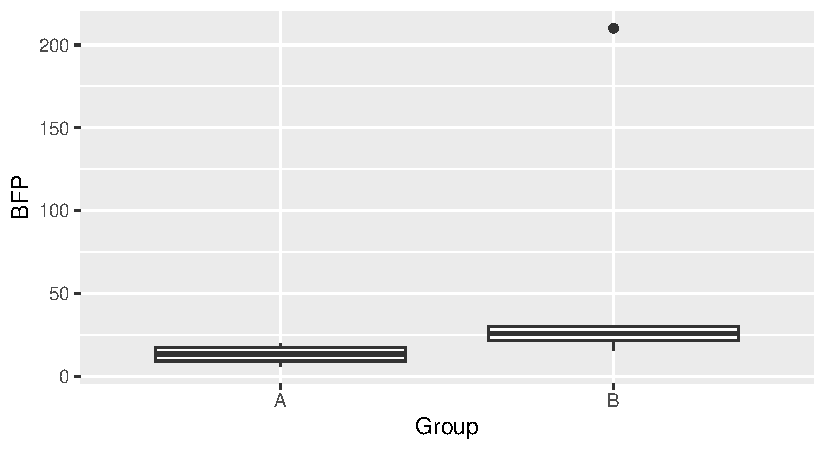
\includegraphics{r_intro_files/figure-pdf/fig-r-workflow-graph-01-1.pdf}

}

\caption{\label{fig-r-workflow-graph-01}Darstellung der Beispieldaten
mittels eines Boxplots mit dem problematischen Datenpunkt.}

\end{figure}%

Im Boxplot in Abbildung Figure~\ref{fig-r-workflow-graph-01} ist der
problematische Datenpunkt noch klarer ersichtlich und er verhindert
gleichzeitig eine Analyse der Daten. Da wir keine weitere Information
haben, durch welchen Wert wir den fehlerhaften Wert ersetzen könnten,
schließen wir den Datenpunkt der Einfachheit halber aus. Dazu benutzen
wir aus dem Paket \texttt{dplyr} die Funktion \texttt{filter()}.

\begin{Shaded}
\begin{Highlighting}[]
\SpecialCharTok{\textgreater{}} \FunctionTok{library}\NormalTok{(dplyr)}
\SpecialCharTok{\textgreater{}}\NormalTok{ bfp\_clean }\OtherTok{\textless{}{-}} \FunctionTok{filter}\NormalTok{(bfp, BFP }\SpecialCharTok{\textless{}=} \DecValTok{100}\NormalTok{)}
\SpecialCharTok{\textgreater{}}\NormalTok{ bfp\_clean}
\end{Highlighting}
\end{Shaded}

\begin{verbatim}
# A tibble: 12 x 2
   Group   BFP
   <chr> <dbl>
 1 A      13.3
 2 A       6  
 3 A      20  
 4 A       8  
 5 A      14  
 6 A      19  
 7 B      22  
 8 B      16  
 9 B      21.7
10 B      30  
11 B      26  
12 B      30  
\end{verbatim}

\begin{Shaded}
\begin{Highlighting}[]
\SpecialCharTok{\textgreater{}} \FunctionTok{ggplot}\NormalTok{(bfp\_clean, }\FunctionTok{aes}\NormalTok{(Group, BFP)) }\SpecialCharTok{+} \FunctionTok{geom\_boxplot}\NormalTok{()}
\end{Highlighting}
\end{Shaded}

\begin{figure}[H]

\centering{

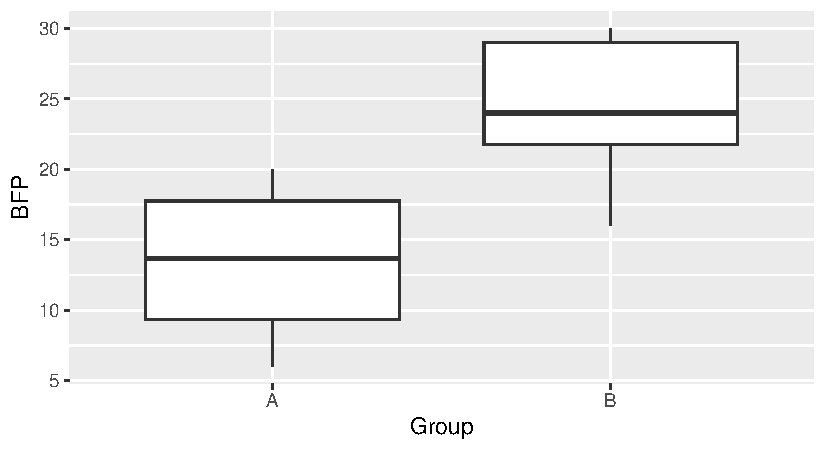
\includegraphics{r_intro_files/figure-pdf/fig-r-workflow-graph-02-1.pdf}

}

\caption{\label{fig-r-workflow-graph-02}Darstellung der Beispieldaten
unter Ausschluss des fehlerhaften Datenpunktes.}

\end{figure}%

Die graphische Darstellung mittels eine Boxplots ist jetzt schon
deutlich aussagekräftiger (siehe Abbildung
Figure~\ref{fig-r-workflow-graph-02}). Ohne jetzt weiter auf
statistische Voraussetzungen einzugehen führen wir jetzt einen
unabhängigen t-Test für Gruppen mit unterschiedlichen Varianzen. Dazu
benutzen wir wieder eine Funktion aus R.

\begin{Shaded}
\begin{Highlighting}[]
\SpecialCharTok{\textgreater{}} \FunctionTok{t.test}\NormalTok{(BFP }\SpecialCharTok{\textasciitilde{}}\NormalTok{ Group, }\AttributeTok{data =}\NormalTok{ bfp\_clean)}
\end{Highlighting}
\end{Shaded}

\begin{verbatim}

    Welch Two Sample t-test

data:  BFP by Group
t = -3.4017, df = 9.9886, p-value = 0.006762
alternative hypothesis: true difference in means between group A and group B is not equal to 0
95 percent confidence interval:
 -18.040619  -3.759381
sample estimates:
mean in group A mean in group B 
       13.38333        24.28333 
\end{verbatim}

Wir dieses Beispiel zeigt, lässt sich in R mittels weniger Befehle eine
Datenanalyse realisieren. Die Entwickler von R haben dabei darauf
geachtet, dass die Namensgebung von Funktionen möglichst nahe an der
gewünschten Tätigkeit liegt, so dass einen der englische Begriff meist
schnell die Funktion herleiten lässt. Im Beispiel haben wir alle Befehlt
direkt auf der Kommandozeile eingegeben und die Daten interaktiv
analysiert. Bei einer tatsächlichen Analyse wird die Datenanalyse aus
einer Kombination von interaktiven Arbeiten und permanenten Skripten
bestehen. Beispielsweise würde diejenigen finalen Befehl die auf die
Daten angewendet werden sollen in eine Skriptdatei geschrieben werden,
so dass die Analyse zu einem späteren Zeitpunkt wieder aufgegriffen bzw.
nachvollziehbar ist. So könnte der gezeigte Workflow in das folgende
Skript münden:

\begin{Shaded}
\begin{Highlighting}[]
\CommentTok{\# Notwendige Bibliotheken}
\FunctionTok{library}\NormalTok{(readr)}
\FunctionTok{library}\NormalTok{(ggplot2)}
\FunctionTok{library}\NormalTok{(dplyr)}

\CommentTok{\# Daten einlesen}
\NormalTok{bfp }\OtherTok{\textless{}{-}} \FunctionTok{read\_csv}\NormalTok{(}\AttributeTok{file =} \StringTok{\textquotesingle{}bfp\_data.txt\textquotesingle{}}\NormalTok{)}

\CommentTok{\# Daten bearbeiten}
\NormalTok{bfp\_clean }\OtherTok{\textless{}{-}} \FunctionTok{filter}\NormalTok{(bfp, BFP }\SpecialCharTok{\textless{}=} \DecValTok{100}\NormalTok{)}

\CommentTok{\# Deskriptiv}
\FunctionTok{summary}\NormalTok{(bfp\_clean)}

\CommentTok{\# Graphiken}
\FunctionTok{ggplot}\NormalTok{(bfp\_clean, }\FunctionTok{aes}\NormalTok{(Group, BFP)) }\SpecialCharTok{+} \FunctionTok{geom\_boxplot}\NormalTok{()}

\CommentTok{\# Analyse}
\FunctionTok{t.test}\NormalTok{(BFP}\SpecialCharTok{\textasciitilde{}}\NormalTok{Group, }\AttributeTok{data =}\NormalTok{ bfp\_clean)}
\end{Highlighting}
\end{Shaded}

Die Abfolge der Befehle in dem Skript sind durch die Verwendung von
Kommentaren, die in \texttt{R} mit einem \texttt{\#} signalisiert
werden, noch besser nachvollziehbar. Dieses Skript könnte zusammen mit
den Daten abgespeichert werden und bleibt dann zu jedem Zeitpunkt
ausführbar.

\chapter{\texorpdfstring{Variablen und Datentypen in
\texttt{R}}{Variablen und Datentypen in R}}\label{variablen-und-datentypen-in-r}

Wie bereits angedeutet, der Umgang mit \texttt{R} besteht vor allem in
der Benutzung von bestimmten Befehlen. Die Befehle, auch Anweisungen
genannt, werden \texttt{R} auf der Kommandozeile übergeben, \texttt{R}
liest die Anweisungen ein und führt entsprechende Operationen durch. Im
einfachsten Fall, kann \texttt{R} beispielsweise als ein
überproportionierter Taschenrechner verwendet werden. In R-Studio ist
die Kommandozeile üblicherweise unten-links zu sehen und signalisiert
durch das Prompt \texttt{\textgreater{}} die Bereitschaft an Befehle
anzunehmen. Beispielsweise führt auf der \texttt{R} Kommandozeile der
folgende Befehl \texttt{2\ +\ 2} gefolgt von einem \texttt{ENTER} zu
folgender Ausgabe:

\begin{Shaded}
\begin{Highlighting}[]
\SpecialCharTok{\textgreater{}} \DecValTok{2} \SpecialCharTok{+} \DecValTok{2}
\end{Highlighting}
\end{Shaded}

\begin{verbatim}
[1] 4
\end{verbatim}

Das \texttt{{[}1{]}} kennzeichnet die erste Zeile des von \texttt{R}
generierten Outputs.

Die Kommandozeile in \texttt{R} funktioniert nach dem Prinzip einer
sogenannten \emph{REPL}. \emph{REPL} ist eine Abkürzung für die
englischen Begriffe read-eval-print loop. Die Eingabe wird durch
\texttt{R} eingelesen (R), im Rahmen der Programmiersprache evaluiert
(E), das Ergebnis wird ausgegeben (P) und anschließend geht die
Kommandozeile zurück zum Ausgangszustand (L). \texttt{R} liest die
Eingabe \texttt{2\ +\ 2}, evaluiert diese Eingabe, dies führt zu dem
Ergebnis \texttt{4}, das Ergebnis wird auf der Kommandozeile ausgegeben,
und \texttt{R} wartet nun wieder auf die nächste Eingabe
\texttt{\textgreater{}}. Wenig überraschend, führt die Eingabe
\texttt{3\ *\ 3} zu folgenden Ablauf.

\begin{Shaded}
\begin{Highlighting}[]
\SpecialCharTok{\textgreater{}} \DecValTok{3} \SpecialCharTok{*} \DecValTok{3}
\end{Highlighting}
\end{Shaded}

\begin{verbatim}
[1] 9
\end{verbatim}

In R-Studio gibt es einen short-cut um in die Kommandozeile zu springen
\texttt{STRG+2}.

In der Kommandozeile in \texttt{R} ist es nach der Ausführung eines
Befehlt nicht möglich mit dem Cursor wieder nach oben zu gehen und bei
einer fehlerhaften Eingabe diese zu berichten. Sondern der komplette
Befehl muss noch einmal eingegeben werden. Allerdings merkt sich
R-Studio die Befehlt und mit den Pfeiltasten \texttt{UP} und
\texttt{DOWN} können diese wieder aufgerufen werden und entsprechend
angepasst werden.

Die Anweisungen \texttt{2\ +\ 2} oder \texttt{3\ *\ 3} werden allgemein
als \textbf{Ausdrücke} bezeichnet. Wir könnten die Beispiele jetzt mit
den üblichen Grundrechenarten \texttt{+-/*} weiterführen, aber es würde
nichts Neues dazukommen. Daher schauen wir uns jetzt an, wie wir
komplexere, mehrstufige Berechnungen durchführen können. Dazu schauen
wir uns ein zentrales Konzept von Programmiersprachen an: Variablen.

\section{\texorpdfstring{Variablen in
\texttt{R}}{Variablen in R}}\label{variablen-in-r}

Nehmen wir, wir wollen das Ergebnis der letzten komplexen Berechnung, in
irgendeiner Form weiter verwenden. Die im Beispiel berechnete \texttt{9}
steht jetzt allerdings für die weitere Bearbeitung nicht mehr zur
Verfügung. \texttt{R} hat die REPL ausgeführt, die Berechnung der
\texttt{9}, und da jetzt mit dieser Ausgabe nichts weiteres durchgeführt
wurde, ist die Ausgabe auch nirgends gespeichert worden. Die Ausgabe
bzw. das Ergebnis eines Befehlt wird als
Rückgabewert\index{Rückgabewert} bezeichnet. Um den Rückgabewert eines
Ausdrucks weiter zu bearbeiten, muss dieser Wert in irgendeiner Form
\texttt{R} zugänglich gemacht werden, d.h. der Rückgabewert muss
irgendwie gespeichert werden. Um Werte weiter verwenden zu kommen, wird
den Werten daher ein Bezeichner, ein Name, zugewiesen. Es wird eine
Variable eingeführt. Erfahrungsgemäß stellt dieses Konzept eine erste
Größe Hürde im Umgang mit \texttt{R}da, das diese Konzept beispielweise
in Tabellenkalkulationsprogrammen, bei denen die Berechnungen scheinbar
direkt auf den zu sehenden Daten stattfindet, nicht vorhanden ist.
Letztendlich ist eine Variable aber nichts als ein Wert in \texttt{R}
dem ein Name zugewiesen wurde.

Um in \texttt{R} einem Ausdruck bzw. dessen Rückgabewert einen Namen
zuzuweisen wird ein spezieller in \texttt{R} definierter Befehl
verwendet, der Zuweisungsoperator \texttt{\textless{}-}. Möchte ich
beispielsweise das Ergebnis der „komplexen`` Berechnung \texttt{3\ *\ 3}
später weiter verwenden, dann verwende ich den Zuweisungsoperator
\texttt{\textless{}-} um dem Rückgabewert einen Namen zu geben.

\begin{Shaded}
\begin{Highlighting}[]
\SpecialCharTok{\textgreater{}}\NormalTok{ wert\_1 }\OtherTok{\textless{}{-}} \DecValTok{3} \SpecialCharTok{*} \DecValTok{3}
\end{Highlighting}
\end{Shaded}

\texttt{R} jetzte keinen Ausdruck mehr zurück, da das Ergebnis des
Zuweisungsoperator die Zuweisung eines Namens ist, was keinen Wert
zurückgibt mehr ergibt. Intern hat \texttt{R} die Berechnung
durchgeführt und dem Rückgabewert den Namen \texttt{wert\_1} zugewiesen.
Der Name ist dabei, im Rahmen bestimmter Konventionen vollkommen
willkührlich und \texttt{R} hätte mich nicht daran gehindert
\texttt{wert\_2}, \texttt{wert\_123}, \texttt{thomas}, \texttt{steffie}
oder einen anderen Namen zu verwenden.

Dies Frage stellt sich jetzt natürlich, wie komme ich meinen berechneten
Wert wieder heran. Einfach indem ich den Bezeichner, den Namen,
\texttt{wert\_1} an \texttt{R} übergebe.

\begin{Shaded}
\begin{Highlighting}[]
\SpecialCharTok{\textgreater{}}\NormalTok{ wert\_1}
\end{Highlighting}
\end{Shaded}

\begin{verbatim}
[1] 9
\end{verbatim}

In R-Studio, gibt es oben-rechts einen Reiter mit der Aufschrift
\textbf{Environment}, hier sollte jetzt auch ein Eintrag zu finden sein
mit dem Bezeichner \texttt{wert\_1} und dem angehängten Wert \(9\).

Dieser Prozess funktionert genau gleich mit einem komplexeren Ausdruck
wie \texttt{2\ +\ 2\ *\ 4}.

\begin{Shaded}
\begin{Highlighting}[]
\SpecialCharTok{\textgreater{}}\NormalTok{ x }\OtherTok{\textless{}{-}} \DecValTok{2} \SpecialCharTok{+} \DecValTok{2} \SpecialCharTok{*} \DecValTok{4}
\end{Highlighting}
\end{Shaded}

Aufruf des Bezeichners \texttt{x} von auf der Kommandozeile führt dann
entsprechend wieder zu der Ausgabe des Wertes.

\begin{Shaded}
\begin{Highlighting}[]
\SpecialCharTok{\textgreater{}}\NormalTok{ x}
\end{Highlighting}
\end{Shaded}

\begin{verbatim}
[1] 10
\end{verbatim}

Konzeptionell stellt sich der Vorgang der Zuweisung in etwa so dar. Im
internen Speicher von \texttt{R} wird der Wert \(10\) an einer passen
Stelle abgespeichert und in einer Tabelle wird ein Eintrag mit dem
Bezeichner \texttt{x} zusammen mit der Adresse des Wertes \(10\)
abgelegt. Wenn \texttt{R} dann auf den Bezeichner \texttt{x} trifft,
dann schaut es in der Tabelle nach, an welcher Stellt sich der Wert
befindet und gibt diesen aus. Dies hat zur Folge, dass Bezeichner
genauso wieder in Ausdrücken verwendet werden können wie Werte.
\texttt{R} ersetzt den jeweiligen Bezeichner mit dem hinterlegten Wert
und führt den Ausdruck aus.

\begin{Shaded}
\begin{Highlighting}[]
\SpecialCharTok{\textgreater{}}\NormalTok{ x }\SpecialCharTok{+}\NormalTok{ wert\_1}
\end{Highlighting}
\end{Shaded}

\begin{verbatim}
[1] 19
\end{verbatim}

\texttt{R} ersetzt den Bezeichner \texttt{x} mit dem Wert \(10\) und den
Bezeichner \texttt{wert\_1} mit dem Wert \(9\) und addiert die beiden
Werte zusammen.

In dieser Vorgehensweise besteht ein grundlegender Unterschied zur der
Arbeitsweise mit Tabellenprogrammen bei denen immer direkt auf den
jeweiligen Zellen gearbeitet wird. In \texttt{R} werden Berechnungen,
die Rückgabewerte von Ausdrücken, Bezeichner zugewiesen und können dann
in späteren Ausdrücken (Befehlen) wieder aufgerufen werden. Anders
herum, wenn Zwischenergebnisse keinen Bezeichner haben, können sie auch
nicht wiederverwendet werden.

Zwei weitere Erläuterungen zu den bisherigen Beispielen sind notwendig.
In den bisherigen Ausdrücken sind Leerzeichen zwischen die einzelnen
Teile der Ausdrücke gesetzt worden. Diese Leerzeichen dienen lediglich
der Leserlichkeit und haben keinen Einfluss auf die Evaluierung des
Ausdrucks durch \texttt{R}. Daher sind die Ausdrücke
\texttt{2\ +\ 2\ *\ 4} und \texttt{2+2*4} äquivalent und führen zum
gleichen Ergebnis. Bei der Ausgabe des Wertes ist wahrscheinlich auch
aufgefallen, das \texttt{R} nicht den Wert \(16\) berechnet hat, der
korrekt wäre, wenn die Evaluierung des Ausdrucks streng von links nach
rechts durchgeführt wird \texttt{2\ +\ 2\ *\ 4\ =\ 4\ *\ 4\ =\ 16}.
\texttt{R} hat jedoch die korrekte mathematischen Regel Punkt-vor-Strich
angewendet und ist daher zum korrekten Ergebnis \texttt{10} gekommen.

\begin{tcolorbox}[enhanced jigsaw, bottomrule=.15mm, breakable, leftrule=.75mm, left=2mm, toptitle=1mm, opacitybacktitle=0.6, bottomtitle=1mm, colframe=quarto-callout-important-color-frame, titlerule=0mm, colback=white, colbacktitle=quarto-callout-important-color!10!white, toprule=.15mm, opacityback=0, arc=.35mm, rightrule=.15mm, title=\textcolor{quarto-callout-important-color}{\faExclamation}\hspace{0.5em}{Important}, coltitle=black]

In \texttt{R} wird bei Bezeichnern zwischen Groß- und Kleinschreibung
unterscheidet. Daher führt der Aufruf des Bezeichners \texttt{X} zu
einem Fehler.

\begin{Shaded}
\begin{Highlighting}[]
\SpecialCharTok{\textgreater{}}\NormalTok{ X}
\end{Highlighting}
\end{Shaded}

\begin{verbatim}
Error in eval(expr, envir, enclos): Objekt 'X' nicht gefunden
\end{verbatim}

Die Fehlermeldung von \texttt{R} gibt auch direkt an, was das Problem
ist, das nämlich kein Objekt mit der Bezeichnung \texttt{X} gefunden
werden kann.

\end{tcolorbox}

\begin{tcolorbox}[enhanced jigsaw, bottomrule=.15mm, breakable, leftrule=.75mm, left=2mm, toptitle=1mm, opacitybacktitle=0.6, bottomtitle=1mm, colframe=quarto-callout-tip-color-frame, titlerule=0mm, colback=white, colbacktitle=quarto-callout-tip-color!10!white, toprule=.15mm, opacityback=0, arc=.35mm, rightrule=.15mm, title=\textcolor{quarto-callout-tip-color}{\faLightbulb}\hspace{0.5em}{Tip}, coltitle=black]

Das Auftreten von Fehler führt bei R Neueinsteigerinnen oft zu großer
Verwirrung ist aber im Programmieralltag ein vollkommen normales
Ereignis und sollte daher niemanden aus der Ruhe bringen. Im
vorliegenden Fall bemängelt R lediglich das es den Bezeichner X nicht
finden kann und dementsprechend nicht weiß wie es weiter verfahren soll.

\end{tcolorbox}

Damit haben wir jetzt das erste große Konzept in \texttt{R}, bzw. in
allen Programmiersprachen, das der \textbf{Variable} kennengelernt. Als
nächstes wenden wir uns dem Konzept der Funktionen in \texttt{R} zu.

\section{\texorpdfstring{Funktionen in
\texttt{R}}{Funktionen in R}}\label{funktionen-in-r}

Ein gutes Template für Funktionen in Programmiersprachen sind Funktionen
aus der Mathematik.

\begin{equation*}
y = f(x)
\end{equation*}

Wir haben eine Funktion \(f()\), dieser Funktion übergeben wir ein
Argument (auch Parameter) \(x\). Die Funktion \(f()\) macht dann etwas
mit diesem Parameter und gibt einen Rückgabewert \(y\) zurück. Sei zum
Beispiel die folgenden Funktion definiert.

\begin{equation*}
f(x) = x^2
\end{equation*}

D.h. der Funktion \(f()\) wird der Parameter \(x\) übergeben. Dieser
Wert wird anschließend quadriert und das Ergebnis der Berechnung wird
zurück gegeben.

In \texttt{R} werden Funktionen nach dem Muster (,,\ldots,) aufgerufen
(die Zeichen \textless\textgreater{} stehen für einen beliebigen
Bezeichner). D.h. sobald ein rundes Klammerpaar auf einen Bezeichner
folgt, geht \texttt{R} davon aus, dass die Anwenderin eine Funktion
aufrufen möchte. Über ,,\ldots, können der Funktion durch Komma
getrennte Parameter übergeben werden. Die Anzahl der Parameter hängt
dabei von der Definition der Funktion ab. In der Mathematik wäre ein
Beispiel eine Funktion mit zwei Argumenten.

\begin{equation*}
f(x,y) = x^2 + y^2
\end{equation*}

\subsection{Funktionen anwenden}\label{funktionen-anwenden}

Ein einfaches Beispiel ist die Anwendung der Wurzelfunktion auf einen
numerischen Wert. In \texttt{R} gibt es schon eine vordefinierte
Funktion mit dem Bezeichner \texttt{sqrt()}, welche die Wurzel des
übergebenen Parameters berechnet.

\begin{Shaded}
\begin{Highlighting}[]
\SpecialCharTok{\textgreater{}}\NormalTok{ y }\OtherTok{\textless{}{-}} \DecValTok{9}
\SpecialCharTok{\textgreater{}} \FunctionTok{sqrt}\NormalTok{(y)}
\end{Highlighting}
\end{Shaded}

\begin{verbatim}
[1] 3
\end{verbatim}

Im Beispiel wird zunächst dem Wert \(9\) der Bezeichner \texttt{y}
zugewiesen. Dieser wird dann an die Wurzelfunktion \texttt{sqrt()}
übergeben.

Ein etwas näher an der Anwendung liegendes Beispiel wäre beispielsweise
die Berechnung des Mittelwerts oder die Summe der Datenreihe
\((3, 5, 7)\) sein. In \texttt{R} wird eine solche geordnete Reihe von
Zahlen als Vektor repräsentiert. Um einen solchen Vektor zu erstellen
wird wiederum eine Funktion \texttt{c()} (für concatenation) verwendet.

\begin{Shaded}
\begin{Highlighting}[]
\SpecialCharTok{\textgreater{}}\NormalTok{ z }\OtherTok{\textless{}{-}} \FunctionTok{c}\NormalTok{(}\DecValTok{3}\NormalTok{, }\DecValTok{5}\NormalTok{, }\DecValTok{7}\NormalTok{)}
\end{Highlighting}
\end{Shaded}

Mit dieser Anweisung hat \texttt{R} einen Vektor mit den drei Einträgen
erstellt. Wir können jetzt den Mittelwert
\(\bar{z} = \frac{1}{3}\sum_{i=1}^3z_i\) mittels der Funktion
\texttt{mean()} berechnen.

\begin{Shaded}
\begin{Highlighting}[]
\SpecialCharTok{\textgreater{}} \FunctionTok{mean}\NormalTok{(z)}
\end{Highlighting}
\end{Shaded}

\begin{verbatim}
[1] 5
\end{verbatim}

Vielleicht interessiert uns jetzt nicht der Mittelwert sondern die Summe
\(\bar{z} = \sum_{i=1}^3z_i\). Dafür können wir die \texttt{sum()}
Funktion verwenden.

\begin{Shaded}
\begin{Highlighting}[]
\SpecialCharTok{\textgreater{}} \FunctionTok{sum}\NormalTok{(z)}
\end{Highlighting}
\end{Shaded}

\begin{verbatim}
[1] 15
\end{verbatim}

Dies sind jetzt nur einige wenige Beispiele und einer der Skills im
Umgang mit \texttt{R} besteht darin die Namen der Funktion sich zu
merken. Dies kann am schnellesten durch den täglichen Umgang mit
\texttt{R} erlernt werden. Am Besten ab heute.

\subsection{\texorpdfstring{Funktionen in
\texttt{R}-Paketen}{Funktionen in R-Paketen}}\label{funktionen-in-r-paketen}

Sollte sich der Fall ergeben, dass keine geeignete Funktion mit
\texttt{R} mitgeliefert wird, dann können Zusatzfunktionen mittels
sogenannter Pakete installiert werden. Ein Paket kann dabei als eine
Sammlung von Funktionen und Anweisungen angesehen werden mit deren Hilfe
die Funktionalität von \texttt{R} erweitert werden kann. Daher wird
zunächst Information darüber benötigt, in welchem Paket die gewünschte
Funktionalität vorhanden ist. Hierfür reicht meistens eine kurze Suche
mittels Google aus.

Ist das Paket nun bekannt, dann sind zwei Schritte zunächst
durchzuführen. Wobei der 1. Schritt nur beim ersten Mal durchgeführt
werden muss. Zunächst muss das benötigte Paket in der lokalen, d.h.
derjenigen auf dem Rechner laufenden, \texttt{R}-Umgebung installiert
werden, wenn es noch nicht bereits vorher installiert wurde (in
R-Studio: Reiter unten-links \textbf{Packages}).

Ein Paket kann mittels des Befehlt \texttt{install.packages()}
installiert werden. Der Name des Paket muss in Gänsefüßchen an die
Funktion übergeben werden. Wollen wir beispielsweise das Paket
\texttt{performance} installieren, führen wir den folgenden Befehl aus.

\begin{Shaded}
\begin{Highlighting}[]
\SpecialCharTok{\textgreater{}} \FunctionTok{install.packages}\NormalTok{(}\StringTok{"performance"}\NormalTok{)}
\end{Highlighting}
\end{Shaded}

\texttt{R} kontaktiert im Hintergrund den CRAN-Server und lädt das Paket
sowie benötigte Abhängigkeiten automatisch herunter. Wenn alles gut
läuft, dann ist das Paket nun in der lokalen Umgebung
\emph{installiert}. Die Funktionalität des Paket steht jedoch noch nicht
direkt zur Verfügung! Sondern, das Paket muss mit einem weiteren Befehl
in die derzeit aktive Arbeitsumgebung geladen werden.

Um das Paket in die aktive Arbeitsumgebung zu laden wird gibt es zwei
Befehle in \texttt{R}, \texttt{library()} und \texttt{require()}. Bei
\texttt{require()} überprüft \texttt{R} zunächst ob das Paket schon
geladen wurde, während bei \texttt{library()} das Paket einfach geladen
wird. Um die Funktionalität von \texttt{performance} jetzt in der
aktiven Session zu nutzen, kann dementsprechend \texttt{library()}
benutzt werden.

\begin{Shaded}
\begin{Highlighting}[]
\SpecialCharTok{\textgreater{}} \FunctionTok{library}\NormalTok{(performance)}
\end{Highlighting}
\end{Shaded}

Dieser zweite Schritt des Paket laden, muss jedes mal nach einen
Neustart von \texttt{R} wieder durchgeführt werden. Zusatzpakete werden
durch \texttt{R} beim Start nicht automatisch geladen.

\begin{tcolorbox}[enhanced jigsaw, bottomrule=.15mm, breakable, leftrule=.75mm, left=2mm, toptitle=1mm, opacitybacktitle=0.6, bottomtitle=1mm, colframe=quarto-callout-tip-color-frame, titlerule=0mm, colback=white, colbacktitle=quarto-callout-tip-color!10!white, toprule=.15mm, opacityback=0, arc=.35mm, rightrule=.15mm, title=\textcolor{quarto-callout-tip-color}{\faLightbulb}\hspace{0.5em}{Tip}, coltitle=black]

Neue Pakete müssen nur beim ersten Mal neu installiert werden. Danach
immer nur noch entweder mit \texttt{library()} oder \texttt{require()}
geladen werden.

\end{tcolorbox}

Der große Vorteil von \texttt{R}, beziehungsweise von jeder vollwertigen
Programmiersprache, besteht nun darin, dass problemlos eigene Funktion
definiert werden können sollten sich keine bereits fertigen Funktionen
finden lassen. Dies führt dazu, dass ständig neue Funktionalität zu
\texttt{R} hinzugefügt werden kann und mittlerweile kaum eine Disziplin
nicht mit eigenen, spezialisierten Paketen aufwarten kann.

\subsection{Eigene Funktionen
schreiben}\label{eigene-funktionen-schreiben}

Im folgenden wird nur kurz examplarisch das Schreiben eigener Funktionen
gezeigt, da damit deutlich tiefer in die Programmierung mit \texttt{R}
eingestiegen werden muss, als dass zum jetzigen Zeitpunkt notwendig ist.

Wollen wir zum Beispiel eine Funktion schreiben die den gewichteten
Mittelwert aus zwei Werten berechnet mit den Gewichten
\((\frac{1}{3},\frac{2}{3})\):

\begin{equation*}
f(x,y) = \frac{1}{3}x + \frac{2}{3}y
\end{equation*}

Dann könnten wir das in \texttt{R} wie folgt ausdrücken.

\begin{Shaded}
\begin{Highlighting}[]
\SpecialCharTok{\textgreater{}}\NormalTok{ mein\_gewichteter\_mittelwert }\OtherTok{\textless{}{-}} \ControlFlowTok{function}\NormalTok{(x,y) \{ }
\SpecialCharTok{+}\NormalTok{   x}\SpecialCharTok{/}\DecValTok{3} \SpecialCharTok{+} \DecValTok{2}\SpecialCharTok{*}\NormalTok{y}\SpecialCharTok{/}\DecValTok{3} 
\SpecialCharTok{+}\NormalTok{ \}}
\end{Highlighting}
\end{Shaded}

Um eine eigene Funktion zu defineren, muss das \emph{Schlüsselworts}
\texttt{function()} verwendet werden. Wenn \texttt{R} den Ausdruck
\texttt{function} sieht, dann interpretiert es den Ausdruck als
Definition einer neuen Funktion. Auf das Schlüsselwort folgen runde
Klammern \texttt{()} die die benötigten Parameter der Funktion
umschließen. Im Beispiel werden zwei Parameter definiert \(x\) und
\(y\). Die Namen der Parameter sind dabei vollkommen willkürlich und
müssen lediglich zu späteren Ausdruck in der Funktion passen. Es folgen
dann zwei geschweifte Klammern \texttt{\{\}} die den sogenannten
Funktionskörper definieren. Im Funktionskörper ist die Funktionalität
der Funktion hinterlegt. Konkret stehen hier die Ausdrücke mit derer die
Funktion ihren Ergebniswert berechnen kann. Um die Funktion aufrufbar zu
machen, braucht sie wieder einen Bezeichner. Dieser wird mittels des
Zuweisungsoperators \texttt{\textless{}-} definiert. In R-Studio sollte
in der \textbf{Environment} nach dem Ausführen der Anweisung nun ein
Eintrag mit dem Namen \texttt{mein\_gewichteter\_mittelwert} stehen. Der
Name ist wiederum vollkommen willkürlich und es \texttt{R} kontrolliert
nicht ob mein Bezeichner semantisch dem entspricht was die Funktion
berechnet.

Nachdem ich die Funktion definiert habe, kann ich sie wie jeder andere
Funktion aufrufen. Bei Aufrufen der Funktion werden die Parameter
entsprechend der übergegebenen Werte in den Klammern im Funktionskörper
ersetzt. Und \texttt{R} führt die Anweisungen im Funktionskörper aus.
Der Rückgabewert der Funktion ist die letzte Anweisung des
Funktionskörpers. Im vorliegenden Beispiel, da es nur eine Anweisung
gibt, wird dieser Wert zurück gegeben.

\begin{Shaded}
\begin{Highlighting}[]
\SpecialCharTok{\textgreater{}} \FunctionTok{mein\_gewichteter\_mittelwert}\NormalTok{(}\DecValTok{3}\NormalTok{,}\DecValTok{6}\NormalTok{)}
\end{Highlighting}
\end{Shaded}

\begin{verbatim}
[1] 5
\end{verbatim}

\begin{tcolorbox}[enhanced jigsaw, bottomrule=.15mm, breakable, leftrule=.75mm, left=2mm, toptitle=1mm, opacitybacktitle=0.6, bottomtitle=1mm, colframe=quarto-callout-note-color-frame, titlerule=0mm, colback=white, colbacktitle=quarto-callout-note-color!10!white, toprule=.15mm, opacityback=0, arc=.35mm, rightrule=.15mm, title=\textcolor{quarto-callout-note-color}{\faInfo}\hspace{0.5em}{Note}, coltitle=black]

Was die letzte Anweisung für den Rückgabewert bedeutet ist etwas
einfacher zu sehen, wenn wir die Funktion etwas kompliziert schreiben.

\begin{Shaded}
\begin{Highlighting}[]
\SpecialCharTok{\textgreater{}}\NormalTok{ mein\_gewichteter\_mittelwert\_2 }\OtherTok{\textless{}{-}} \ControlFlowTok{function}\NormalTok{(x,y) \{ }
\SpecialCharTok{+}\NormalTok{   a }\OtherTok{\textless{}{-}}\NormalTok{ x}\SpecialCharTok{/}\DecValTok{3}
\SpecialCharTok{+}\NormalTok{   b }\OtherTok{\textless{}{-}} \DecValTok{2}\SpecialCharTok{*}\NormalTok{y}\SpecialCharTok{/}\DecValTok{3}
\SpecialCharTok{+}\NormalTok{   a }\SpecialCharTok{+}\NormalTok{ b}
\SpecialCharTok{+}\NormalTok{ \}}
\SpecialCharTok{\textgreater{}} \FunctionTok{mein\_gewichteter\_mittelwert\_2}\NormalTok{(}\DecValTok{3}\NormalTok{,}\DecValTok{6}\NormalTok{)}
\end{Highlighting}
\end{Shaded}

\begin{verbatim}
[1] 5
\end{verbatim}

Hier haben wir mit \texttt{a} und \texttt{b} zunächst zwei
Zwischenberechnung durchgeführt und dann in der letzten Anweisung das
Ergebnis für den Rückgabewert berechnet.

\end{tcolorbox}

Wer tiefer in die Programmierung von Funktion in \texttt{R} einsteigen
möchte, sollte sich \href{https://r4ds.hadley.nz/functions.html}{R4DS}
und \href{https://adv-r.hadley.nz/functions.html}{Advanced R} anschauen.

\section{Datentypen}\label{datentypen}

Um mit \texttt{R} effektiv zu arbeiten ist ein zumindest oberflächliches
Verständnis von sogenannten Datentypen notwendig. Konzeptionell sind
Datentypen Eigenschaften von Werten die bestimmen welche Operationen mit
diesem Wert möglich sind. Der einfachste Datentyp numerisch erlaubt zum
Beispiel die üblichen mathematischen Operationen \texttt{+-/*} die wir
bereits kennengelernt haben. Eine Zeichenkette \texttt{"Haus"} lässt
sich dagegen nicht dividieren. Die Werte können auch als Objekte
bezeichnet werden, was konzeptionell einfacher nachzuvollziehen. Den
Datentypen eines Objektes kann mittels der Funktion \texttt{typeof()}
bestimmt werden. Ein Objekt hat einen Typ und einen Wert. Wir beginnen
mit den grundlegendsten, den atomaren (atomic), Datentypen: Numerisch,
Zeichenketten und logische Werte.

\subsection{Numerisch}\label{numerisch}

Wie bereits beschreiben, ist einer der einfachsten Datentypen ein
numerischer Wert wie \texttt{1}, \texttt{123345} \texttt{12.3456}. Es
gibt noch eine Unterscheidung in \texttt{R} zwischen ganzzahligen Werten
(integer) und Dezimalzahlen (double), wobei für die meisten
Anwendungsfälle die Unterscheidung nicht von großer Bedeutung ist. Das
Dezimaltrennzeichen in \texttt{R} ist ein Punkt \texttt{.}.

\begin{Shaded}
\begin{Highlighting}[]
\SpecialCharTok{\textgreater{}}\NormalTok{ dezimal\_zahl }\OtherTok{\textless{}{-}} \FloatTok{12.345}
\SpecialCharTok{\textgreater{}}\NormalTok{ dezimal\_zahl}
\end{Highlighting}
\end{Shaded}

\begin{verbatim}
[1] 12.345
\end{verbatim}

\begin{Shaded}
\begin{Highlighting}[]
\SpecialCharTok{\textgreater{}} \FunctionTok{typeof}\NormalTok{(dezimal\_zahl)}
\end{Highlighting}
\end{Shaded}

\begin{verbatim}
[1] "double"
\end{verbatim}

\begin{Shaded}
\begin{Highlighting}[]
\SpecialCharTok{\textgreater{}} \FunctionTok{typeof}\NormalTok{(}\FloatTok{12.345}\NormalTok{)}
\end{Highlighting}
\end{Shaded}

\begin{verbatim}
[1] "double"
\end{verbatim}

Integer Werte werden in \texttt{R} mit einem angehängtem \texttt{L}
spezifiziert. Wir kein \texttt{L} angehängt geht \texttt{R} per default
bei Zahlen immer von einer Dezimalzahl aus.

\begin{Shaded}
\begin{Highlighting}[]
\SpecialCharTok{\textgreater{}}\NormalTok{ ganz\_zahl }\OtherTok{\textless{}{-}} \DecValTok{12345}\NormalTok{L}
\SpecialCharTok{\textgreater{}}\NormalTok{ ganz\_zahl}
\end{Highlighting}
\end{Shaded}

\begin{verbatim}
[1] 12345
\end{verbatim}

\begin{Shaded}
\begin{Highlighting}[]
\SpecialCharTok{\textgreater{}} \FunctionTok{typeof}\NormalTok{(ganz\_zahl)}
\end{Highlighting}
\end{Shaded}

\begin{verbatim}
[1] "integer"
\end{verbatim}

\begin{Shaded}
\begin{Highlighting}[]
\SpecialCharTok{\textgreater{}} \FunctionTok{typeof}\NormalTok{(}\DecValTok{12345}\NormalTok{)}
\end{Highlighting}
\end{Shaded}

\begin{verbatim}
[1] "double"
\end{verbatim}

\begin{Shaded}
\begin{Highlighting}[]
\SpecialCharTok{\textgreater{}} \FunctionTok{typeof}\NormalTok{(}\DecValTok{12345}\NormalTok{L)}
\end{Highlighting}
\end{Shaded}

\begin{verbatim}
[1] "integer"
\end{verbatim}

Die numerischen Werte erlauben die üblichen mathematischen Operationen.

\subsection{Zeichenketten (Strings)}\label{zeichenketten-strings}

Der nächste Datentyp sind Zeichenketten (character in den meisten
anderen Programmiersprachen strings). Zeichenketten repräsentieren
Textdaten und werden oft für die Manipulation von Texten und die
Verarbeitung von Zeichen verwendet. Zeichenketten können mit einfachen
Anführungszeichen (\texttt{\textquotesingle{}}) oder doppelten
Anführungszeichen (\texttt{"}) erstellt werden.

\begin{Shaded}
\begin{Highlighting}[]
\SpecialCharTok{\textgreater{}}\NormalTok{ s\_1 }\OtherTok{\textless{}{-}} \StringTok{"Haus"}
\SpecialCharTok{\textgreater{}}\NormalTok{ s\_1}
\end{Highlighting}
\end{Shaded}

\begin{verbatim}
[1] "Haus"
\end{verbatim}

\begin{Shaded}
\begin{Highlighting}[]
\SpecialCharTok{\textgreater{}} \FunctionTok{typeof}\NormalTok{(s\_1)}
\end{Highlighting}
\end{Shaded}

\begin{verbatim}
[1] "character"
\end{verbatim}

In \texttt{R} wird der Typ von Zeichenketten als \texttt{character}
bezeichnet.

Bezüglich der Anführungszeiche, besteht semantisch kein Unterschied
zwischen den einfachen und den doppelten Anführungszeichen und es ist
mehr ein Zeichen persönlicher Präferenz welche Art benutzt wird. Ein
Anwendungsfall wo die Art von Bedeutung ist, erfolgt wenn innerhalb der
Zeichenketten Anführungszeichen benötigt werden. Dann müssen die äußeren
Zeichenketten der jeweils andere Typ sein, da ansonsten \texttt{R} die
Zeichenkette nicht als solche erkennt. Also zum Beispiel wenn ich als
Zeichenkette den Wert: \texttt{Er\ sagte:\ "Nein"!}, benötige, verwende
ich die einfachen Anführungszeichen um \texttt{R} zu signalisieren das
ich eine Zeichenkette benötige.

\begin{Shaded}
\begin{Highlighting}[]
\SpecialCharTok{\textgreater{}}\NormalTok{ s\_2 }\OtherTok{\textless{}{-}} \StringTok{\textquotesingle{}Er sagte: "Nein"!\textquotesingle{}}
\SpecialCharTok{\textgreater{}}\NormalTok{ s\_2}
\end{Highlighting}
\end{Shaded}

\begin{verbatim}
[1] "Er sagte: \"Nein\"!"
\end{verbatim}

Um Operationen auf Zeichenketten anzuwenden gibt es in \texttt{R} eine
ganze Reihe von spezialisierten Funktionen. Möchte ich zum Beispiel
einen Teil der Zeichen aus einer Zeichenkette extrahieren, kann ich die
\texttt{substring()}-Funktion verwenden.

\begin{Shaded}
\begin{Highlighting}[]
\SpecialCharTok{\textgreater{}}\NormalTok{ s\_3 }\OtherTok{\textless{}{-}} \StringTok{"DasisteinelangeZeichenkette"}
\SpecialCharTok{\textgreater{}} \FunctionTok{substring}\NormalTok{(s\_3, }\DecValTok{4}\NormalTok{, }\DecValTok{6}\NormalTok{)}
\end{Highlighting}
\end{Shaded}

\begin{verbatim}
[1] "ist"
\end{verbatim}

Der erste Parameter übergibt die Zeichenkette an \texttt{substring()}
während der zweiter Parameter den Startposition und der dritte Parameter
die Endposition des zu extrahierenden Strings angibt.

Die Länge einer Zeichenkette kann mit der Funktion \texttt{nchar()}
bestimmt werden.

\begin{Shaded}
\begin{Highlighting}[]
\SpecialCharTok{\textgreater{}} \FunctionTok{nchar}\NormalTok{(s\_3)}
\end{Highlighting}
\end{Shaded}

\begin{verbatim}
[1] 27
\end{verbatim}

Eine Funktion die oft mit Zeichenketten eine Anwendung findet ist die
\texttt{paste()} bzw. die Spezialform \texttt{paste0()}. Mit
\texttt{paste()} können Zeichenkette zusammengesetzt werden.

\begin{Shaded}
\begin{Highlighting}[]
\SpecialCharTok{\textgreater{}} \FunctionTok{paste}\NormalTok{(}\StringTok{\textquotesingle{}Ich\textquotesingle{}}\NormalTok{, }\StringTok{\textquotesingle{}bin\textquotesingle{}}\NormalTok{, }\StringTok{\textquotesingle{}ein\textquotesingle{}}\NormalTok{, }\StringTok{\textquotesingle{}Berliner\textquotesingle{}}\NormalTok{)}
\end{Highlighting}
\end{Shaded}

\begin{verbatim}
[1] "Ich bin ein Berliner"
\end{verbatim}

Per default fügt \texttt{paste()} ein Leerzeichen zwischen die
Zeichenketten ein. Dies kann entsprechend angepasst werden.

\begin{Shaded}
\begin{Highlighting}[]
\SpecialCharTok{\textgreater{}} \FunctionTok{paste}\NormalTok{(}\StringTok{\textquotesingle{}Ich\textquotesingle{}}\NormalTok{, }\StringTok{\textquotesingle{}bin\textquotesingle{}}\NormalTok{, }\StringTok{\textquotesingle{}ein\textquotesingle{}}\NormalTok{, }\StringTok{\textquotesingle{}Kölner\textquotesingle{}}\NormalTok{, }\AttributeTok{sep =} \StringTok{\textquotesingle{}{-}{-}\textquotesingle{}}\NormalTok{)}
\end{Highlighting}
\end{Shaded}

\begin{verbatim}
[1] "Ich--bin--ein--Kölner"
\end{verbatim}

Die Argumente an \texttt{paste()} müssen nicht alle Zeichenketten sein,
werden aber dann in Zeichenketten konvertiert.

\begin{Shaded}
\begin{Highlighting}[]
\SpecialCharTok{\textgreater{}} \FunctionTok{paste}\NormalTok{(}\DecValTok{3}\NormalTok{, }\DecValTok{2}\NormalTok{, }\StringTok{\textquotesingle{}{-}mal\textquotesingle{}}\NormalTok{, }\AttributeTok{sep=}\StringTok{\textquotesingle{}\textquotesingle{}}\NormalTok{)}
\end{Highlighting}
\end{Shaded}

\begin{verbatim}
[1] "32-mal"
\end{verbatim}

\texttt{paste0()} ist eine Spezielform von \texttt{paste()} bei der das
Argument \texttt{sep} auf \texttt{""} gesetzt ist. Das heißt, die
Zeichenketten werden direkt aneinander gehängt.

\begin{Shaded}
\begin{Highlighting}[]
\SpecialCharTok{\textgreater{}} \FunctionTok{paste0}\NormalTok{(}\StringTok{\textquotesingle{}kein\textquotesingle{}}\NormalTok{,}\StringTok{\textquotesingle{}zwischen\textquotesingle{}}\NormalTok{,}\StringTok{\textquotesingle{}raum\textquotesingle{}}\NormalTok{)}
\end{Highlighting}
\end{Shaded}

\begin{verbatim}
[1] "keinzwischenraum"
\end{verbatim}

\begin{tcolorbox}[enhanced jigsaw, bottomrule=.15mm, breakable, leftrule=.75mm, left=2mm, toptitle=1mm, opacitybacktitle=0.6, bottomtitle=1mm, colframe=quarto-callout-tip-color-frame, titlerule=0mm, colback=white, colbacktitle=quarto-callout-tip-color!10!white, toprule=.15mm, opacityback=0, arc=.35mm, rightrule=.15mm, title=\textcolor{quarto-callout-tip-color}{\faLightbulb}\hspace{0.5em}{Tip}, coltitle=black]

Das Paket \texttt{stringr} bietet eine große Sammlung von Funktion die
den Umgang und die Manipulation von Zeichenketten stark vereinfachen.

\end{tcolorbox}

\subsection{Logische (Boolean) Werte}\label{logische-boolean-werte}

Der nächste Datentyp sind sogenannte logische Werte oder Wahrheitswerte.
Logische Werte können nur einen von zwei Werten annehmen, entweder WAHR
oder FALSCH. Logische Ausdrücke kennt ihr wahrscheinlich aus der Schule
in Form von Wahrheitstabellen bei denen boolesche Werte entweder mit
\textbf{und} \(\cap\) oder \textbf{oder} \(\cup\) verknüpft werden
(siehe Table~\ref{tbl-r-kickoff-bool}).

\begin{table}

\caption{\label{tbl-r-kickoff-bool}Verknüpfung von Wahrheitswerten mit
und (\(\cap\)) bzw. oder (\(\cup\)).}

\begin{minipage}{0.50\linewidth}

\begin{longtable}[]{@{}lll@{}}
\caption{Verknüpfung mit \(\cap\)}\tabularnewline
\toprule\noalign{}
\(\cap\) & TRUE & FALSE \\
\midrule\noalign{}
\endfirsthead
\toprule\noalign{}
\(\cap\) & TRUE & FALSE \\
\midrule\noalign{}
\endhead
\bottomrule\noalign{}
\endlastfoot
TRUE & TRUE & FALSE \\
FALSE & FALSE & FALSE \\
\end{longtable}

\end{minipage}%
%
\begin{minipage}{0.50\linewidth}

\begin{longtable}[]{@{}lll@{}}
\caption{Verknüpfung mit \(\cup\)}\tabularnewline
\toprule\noalign{}
\(\cup\) & TRUE & FALSE \\
\midrule\noalign{}
\endfirsthead
\toprule\noalign{}
\(\cup\) & TRUE & FALSE \\
\midrule\noalign{}
\endhead
\bottomrule\noalign{}
\endlastfoot
TRUE & TRUE & TRUE \\
FALSE & TRUE & FALSE \\
\end{longtable}

\end{minipage}%

\end{table}%

In \texttt{R} werden die beiden Werte mit \texttt{TRUE} und
\texttt{FALSE} oder in der abgekürzten Form \texttt{T} und \texttt{F}
dargestellt.

\begin{Shaded}
\begin{Highlighting}[]
\SpecialCharTok{\textgreater{}}\NormalTok{ wahr }\OtherTok{\textless{}{-}} \ConstantTok{TRUE}
\SpecialCharTok{\textgreater{}}\NormalTok{ wahr}
\end{Highlighting}
\end{Shaded}

\begin{verbatim}
[1] TRUE
\end{verbatim}

\begin{Shaded}
\begin{Highlighting}[]
\SpecialCharTok{\textgreater{}}\NormalTok{ falsch }\OtherTok{\textless{}{-}} \ConstantTok{FALSE}
\SpecialCharTok{\textgreater{}}\NormalTok{ falsch}
\end{Highlighting}
\end{Shaded}

\begin{verbatim}
[1] FALSE
\end{verbatim}

Die beiden Verknüpfungen werden mit \texttt{\&} für \(\cap\) und
\texttt{\textbar{}} für \(\cup\).

\begin{Shaded}
\begin{Highlighting}[]
\SpecialCharTok{\textgreater{}}\NormalTok{ wahr }\SpecialCharTok{\&}\NormalTok{ wahr}
\end{Highlighting}
\end{Shaded}

\begin{verbatim}
[1] TRUE
\end{verbatim}

\begin{Shaded}
\begin{Highlighting}[]
\SpecialCharTok{\textgreater{}}\NormalTok{ wahr }\SpecialCharTok{\&}\NormalTok{ falsch}
\end{Highlighting}
\end{Shaded}

\begin{verbatim}
[1] FALSE
\end{verbatim}

\begin{Shaded}
\begin{Highlighting}[]
\SpecialCharTok{\textgreater{}}\NormalTok{ falsch }\SpecialCharTok{\&}\NormalTok{ falsch}
\end{Highlighting}
\end{Shaded}

\begin{verbatim}
[1] FALSE
\end{verbatim}

\begin{Shaded}
\begin{Highlighting}[]
\SpecialCharTok{\textgreater{}}\NormalTok{ wahr }\SpecialCharTok{|}\NormalTok{ wahr}
\end{Highlighting}
\end{Shaded}

\begin{verbatim}
[1] TRUE
\end{verbatim}

\begin{Shaded}
\begin{Highlighting}[]
\SpecialCharTok{\textgreater{}}\NormalTok{ wahr }\SpecialCharTok{|}\NormalTok{ falsch}
\end{Highlighting}
\end{Shaded}

\begin{verbatim}
[1] TRUE
\end{verbatim}

\begin{Shaded}
\begin{Highlighting}[]
\SpecialCharTok{\textgreater{}}\NormalTok{ falsch }\SpecialCharTok{|}\NormalTok{ falsch}
\end{Highlighting}
\end{Shaded}

\begin{verbatim}
[1] FALSE
\end{verbatim}

Logische Werte sind vor allem bei der Ablaufkontrolle und beim
Indexieren wichtig.

Logische Werte können in numerische Werte konvertiert (coercion) werden,
dabei wird \texttt{FALSE} zu \(0\) und \texttt{TRUE} zu \(1\). Mit der
Funktion \texttt{as.numeric()} können wir zum Beispiel Objekte von einem
Typ in einen numerischen Typ konvergieren.

\begin{Shaded}
\begin{Highlighting}[]
\SpecialCharTok{\textgreater{}} \FunctionTok{as.numeric}\NormalTok{(wahr)}
\end{Highlighting}
\end{Shaded}

\begin{verbatim}
[1] 1
\end{verbatim}

\begin{Shaded}
\begin{Highlighting}[]
\SpecialCharTok{\textgreater{}} \FunctionTok{as.numeric}\NormalTok{(falsch)}
\end{Highlighting}
\end{Shaded}

\begin{verbatim}
[1] 0
\end{verbatim}

Die umgekehrte Richtung, von numerisch zum logischen Wert, kann mittels
der Funktion \texttt{as.logical()} durchgeführt werden. Dabei werden
alle Werte \(\neq0\) zu WAHR und \(0\) zu FALSCH.

\begin{Shaded}
\begin{Highlighting}[]
\SpecialCharTok{\textgreater{}} \FunctionTok{as.logical}\NormalTok{(}\DecValTok{123}\NormalTok{)}
\end{Highlighting}
\end{Shaded}

\begin{verbatim}
[1] TRUE
\end{verbatim}

\begin{Shaded}
\begin{Highlighting}[]
\SpecialCharTok{\textgreater{}} \FunctionTok{as.logical}\NormalTok{(}\FloatTok{1.23}\NormalTok{)}
\end{Highlighting}
\end{Shaded}

\begin{verbatim}
[1] TRUE
\end{verbatim}

\begin{Shaded}
\begin{Highlighting}[]
\SpecialCharTok{\textgreater{}} \FunctionTok{as.logical}\NormalTok{(}\DecValTok{0}\NormalTok{)}
\end{Highlighting}
\end{Shaded}

\begin{verbatim}
[1] FALSE
\end{verbatim}

Die Konvertierung von einem Datentyp in einen anderen Datentyp passiert
zum Teil auch automatisch. Gebe ich zum Beispiel den foglenden Ausdruck
ein:

\begin{Shaded}
\begin{Highlighting}[]
\SpecialCharTok{\textgreater{}} \DecValTok{1} \SpecialCharTok{\&} \ConstantTok{TRUE}
\end{Highlighting}
\end{Shaded}

\begin{verbatim}
[1] TRUE
\end{verbatim}

Erhalten wir als Ergebnis des Ausdrucks den Wert \texttt{TRUE}. Der
Operator \texttt{\&} kann nur mit logischen Werten arbeiten. Wir haben
aber einen numerischen und einen logischen Wert übergeben. \texttt{R}
versucht daher zunächst den nicht-logischen Wert in einen logischen Wert
zu konvertieren. In dem Falle geht das problemlos da numerische Werte,
wie oben gesprochen, nach der folgenden Regel konvertiert werden.

\begin{equation*}
\text{logical}(x) = \begin{cases}
\text{F}, \text{if } x = 0 \\
\text{T}, \text{if } x \neq 0
\end{cases}
\end{equation*}

Nach dieser Regel wird die \texttt{1} in \texttt{TRUE} konvertiert und
dann der neue Ausdruck \texttt{TRUE\ \&\ TRUE} ausgewertet, der dann
entsprechend zu \texttt{TRUE} führt.

Eine praktische Funktion im Zusammenhang ist logischen Werte,
insbesonderen logischen Vektoren, ist \texttt{which()}. \texttt{which()}
gibt bei einen logischen Vektor die Position der Wert mit dem Wert
\texttt{TRUE}.

\begin{Shaded}
\begin{Highlighting}[]
\SpecialCharTok{\textgreater{}} \FunctionTok{which}\NormalTok{(}\FunctionTok{c}\NormalTok{(}\ConstantTok{TRUE}\NormalTok{, }\ConstantTok{FALSE}\NormalTok{, }\ConstantTok{TRUE}\NormalTok{, }\ConstantTok{FALSE}\NormalTok{, }\ConstantTok{TRUE}\NormalTok{, }\ConstantTok{TRUE}\NormalTok{))}
\end{Highlighting}
\end{Shaded}

\begin{verbatim}
[1] 1 3 5 6
\end{verbatim}

\subsection{Vektoren}\label{vektoren}

Vektoren sind ein grundlegender Datentypein \texttt{R} und können sowohl
numerische als auch nicht-numerische Werte speichern. Allerdings kann
immer nur eine Datentyp in einem Vektor gespeichert werden. Da Vektoren
sehr oft bei Datenanalysen verwendet werden und oft zur
Datenrepräsentation verwendet werden, werden sie entsprechend direkt in
\texttt{R} unterstützt. Etwas allgemeiner betrachtet können Vektoren als
eine geordnete Sammlung von Elementen betrachtet werden. Geordnet
bedeutet dabei, dass sie ein feststehende Abfolge haben.

Die direkteste Art einen Vektoren in \texttt{R} zu erstellen, ist
mittels der \texttt{c()} Funktion \index{c()} (\texttt{c} von combine).
Wollen wir zum Beispiel einen numerischen Vektor mit den folgenden
Einträgen erstellen.

\begin{equation}
v_1 = \begin{pmatrix}3\\7\\8\end{pmatrix}
\end{equation}

Dann sieht dies in \texttt{R} folgendermaßen aus.

\begin{Shaded}
\begin{Highlighting}[]
\SpecialCharTok{\textgreater{}}\NormalTok{ v\_1 }\OtherTok{\textless{}{-}} \FunctionTok{c}\NormalTok{(}\DecValTok{3}\NormalTok{,}\DecValTok{7}\NormalTok{,}\DecValTok{8}\NormalTok{)}
\SpecialCharTok{\textgreater{}}\NormalTok{ v\_1}
\end{Highlighting}
\end{Shaded}

\begin{verbatim}
[1] 3 7 8
\end{verbatim}

Das gleiche Prinzip funktioniert auch mit anderen Typen. Beispielweise
mit einem Zeichenkettenvektor.

\begin{Shaded}
\begin{Highlighting}[]
\SpecialCharTok{\textgreater{}}\NormalTok{ v\_2 }\OtherTok{\textless{}{-}} \FunctionTok{c}\NormalTok{(}\StringTok{\textquotesingle{}mama\textquotesingle{}}\NormalTok{,}\StringTok{\textquotesingle{}papa\textquotesingle{}}\NormalTok{,}\StringTok{\textquotesingle{}tochter\textquotesingle{}}\NormalTok{)}
\SpecialCharTok{\textgreater{}}\NormalTok{ v\_2}
\end{Highlighting}
\end{Shaded}

\begin{verbatim}
[1] "mama"    "papa"    "tochter"
\end{verbatim}

Oder einem logischen Vektor.

\begin{Shaded}
\begin{Highlighting}[]
\SpecialCharTok{\textgreater{}}\NormalTok{ v\_bool }\OtherTok{\textless{}{-}} \FunctionTok{c}\NormalTok{(}\ConstantTok{TRUE}\NormalTok{, }\ConstantTok{TRUE}\NormalTok{, }\ConstantTok{FALSE}\NormalTok{, }\ConstantTok{TRUE}\NormalTok{)}
\end{Highlighting}
\end{Shaded}

Auf einzelne Elemente oder Teile eines Vektor kann mittels des
sogenannten subsettings zugegriffen werden. Jeder Vektor hat eine
definierte Länge die wir mit \texttt{length()} bestimmen können.

\begin{Shaded}
\begin{Highlighting}[]
\SpecialCharTok{\textgreater{}} \FunctionTok{length}\NormalTok{(v\_2)}
\end{Highlighting}
\end{Shaded}

\begin{verbatim}
[1] 3
\end{verbatim}

Mit eckigen Klammern \texttt{{[}{]}} können wir Teilelemente des Vektors
extrahieren. Die Indizierung geht dabei von \(1\) bis \$n = \$
\texttt{length(Vektor)}. Wollen wir zum Beispiel das zweite Element aus
\(v_1\) extrahieren, dann verwenden wir.

\begin{Shaded}
\begin{Highlighting}[]
\SpecialCharTok{\textgreater{}}\NormalTok{ v\_1[}\DecValTok{2}\NormalTok{]}
\end{Highlighting}
\end{Shaded}

\begin{verbatim}
[1] 7
\end{verbatim}

Wenn der Index außerhalb des erlaubten Bereichs ist, dann wird ein
\texttt{NA} für \texttt{(N)ot\ (A)vailable} von \texttt{R}
zurückgegeben.

\begin{Shaded}
\begin{Highlighting}[]
\SpecialCharTok{\textgreater{}}\NormalTok{ v\_1[}\DecValTok{10}\NormalTok{]}
\end{Highlighting}
\end{Shaded}

\begin{verbatim}
[1] NA
\end{verbatim}

\texttt{R} erlaubt die Verwendung von Vektoren zum subsetten. Wenn ich
das 1. und 3. Element aus \(v_2\) extrahieren möchte, kann ich einen
Vektor mit den beiden Elementen \(1\) und \(3\),
\(v_{\text{index}} = (1,3)\) an \texttt{{[}{]}} übergeben.

\begin{Shaded}
\begin{Highlighting}[]
\SpecialCharTok{\textgreater{}}\NormalTok{ v\_i }\OtherTok{\textless{}{-}} \FunctionTok{c}\NormalTok{(}\DecValTok{1}\NormalTok{,}\DecValTok{3}\NormalTok{)}
\SpecialCharTok{\textgreater{}}\NormalTok{ v\_2[v\_i]}
\end{Highlighting}
\end{Shaded}

\begin{verbatim}
[1] "mama"    "tochter"
\end{verbatim}

Das funktioniert ebenfalls ohne den Zwischenvektor.

\begin{Shaded}
\begin{Highlighting}[]
\SpecialCharTok{\textgreater{}}\NormalTok{ v\_2[}\FunctionTok{c}\NormalTok{(}\DecValTok{1}\NormalTok{,}\DecValTok{3}\NormalTok{)]}
\end{Highlighting}
\end{Shaded}

\begin{verbatim}
[1] "mama"    "tochter"
\end{verbatim}

Der zurückgegebene Wert ist dann auch wieder ein Vektor. Wir können
dadurch zum Beispiel einen Vektor erstellen, der länger als der
Ursprungsvektor ist.

\begin{Shaded}
\begin{Highlighting}[]
\SpecialCharTok{\textgreater{}}\NormalTok{ v\_1[}\FunctionTok{c}\NormalTok{(}\DecValTok{1}\NormalTok{,}\DecValTok{1}\NormalTok{,}\DecValTok{2}\NormalTok{,}\DecValTok{2}\NormalTok{,}\DecValTok{3}\NormalTok{,}\DecValTok{3}\NormalTok{)]}
\end{Highlighting}
\end{Shaded}

\begin{verbatim}
[1] 3 3 7 7 8 8
\end{verbatim}

Zum subsetten können auch logische Vektoren verwendet werden. Der
resultierende Vektor ist ein Vektor mit denjenigen Elementen, für die
der logische Vektor den Wert \texttt{TRUE} hat.

\begin{Shaded}
\begin{Highlighting}[]
\SpecialCharTok{\textgreater{}}\NormalTok{ v\_bool }\OtherTok{\textless{}{-}} \FunctionTok{c}\NormalTok{(}\ConstantTok{TRUE}\NormalTok{, }\ConstantTok{FALSE}\NormalTok{, }\ConstantTok{TRUE}\NormalTok{)}
\SpecialCharTok{\textgreater{}}\NormalTok{ v\_1[v\_bool]}
\end{Highlighting}
\end{Shaded}

\begin{verbatim}
[1] 3 8
\end{verbatim}

Wird ein negativer Wert an \texttt{{[}{]}} übergeben, dann wird dieser
bzw. diese Wert(e) von \texttt{R} ausgeschlossen.

\begin{Shaded}
\begin{Highlighting}[]
\SpecialCharTok{\textgreater{}}\NormalTok{ v\_1[}\SpecialCharTok{{-}}\DecValTok{2}\NormalTok{]}
\end{Highlighting}
\end{Shaded}

\begin{verbatim}
[1] 3 8
\end{verbatim}

Das funktioniert auch wieder mit Vektoren.

\begin{Shaded}
\begin{Highlighting}[]
\SpecialCharTok{\textgreater{}}\NormalTok{ v\_lang }\OtherTok{\textless{}{-}} \FunctionTok{c}\NormalTok{(}\DecValTok{1}\NormalTok{,}\DecValTok{2}\NormalTok{,}\DecValTok{3}\NormalTok{,}\DecValTok{4}\NormalTok{,}\DecValTok{5}\NormalTok{,}\DecValTok{6}\NormalTok{,}\DecValTok{7}\NormalTok{)}
\SpecialCharTok{\textgreater{}}\NormalTok{ v\_lang[}\SpecialCharTok{{-}}\FunctionTok{c}\NormalTok{(}\DecValTok{2}\NormalTok{,}\DecValTok{3}\NormalTok{,}\DecValTok{6}\NormalTok{)]}
\end{Highlighting}
\end{Shaded}

\begin{verbatim}
[1] 1 4 5 7
\end{verbatim}

Bei all diesen Anwendungen ist immer darauf zu achten, dass solange
keine Zuweisung mittels \texttt{\textless{}-} ausgeführt, der jeweilige
Vektor nicht verändert wird.

Auf numerische Vektoren können die gängigen mathematischen Operatoren
(\texttt{+-*/}) angewendet werden. Die Operationen werden elementweise
ausgeführt.

\begin{equation*}
\begin{pmatrix}v_1\\v_2\\\vdots\\v_n\end{pmatrix} \times
\begin{pmatrix}a\\b\\\vdots\\c\end{pmatrix} = 
\begin{pmatrix}av_1\\bv_2\\\vdots\\cv_n\end{pmatrix} \cdot
\end{equation*}

Dementsprechend können Vektoren auch addiert werden, wenn die Längen
gleich sind. Die Addition erfolgt dann ebenfalls elementweise.

\begin{Shaded}
\begin{Highlighting}[]
\SpecialCharTok{\textgreater{}}\NormalTok{ v\_3 }\OtherTok{\textless{}{-}} \FunctionTok{c}\NormalTok{(}\DecValTok{1}\NormalTok{,}\DecValTok{2}\NormalTok{,}\DecValTok{3}\NormalTok{)}
\SpecialCharTok{\textgreater{}}\NormalTok{ v\_4 }\OtherTok{\textless{}{-}} \FunctionTok{c}\NormalTok{(}\DecValTok{4}\NormalTok{,}\DecValTok{5}\NormalTok{,}\DecValTok{6}\NormalTok{)}
\SpecialCharTok{\textgreater{}}\NormalTok{ v\_3 }\SpecialCharTok{+}\NormalTok{ v\_4}
\end{Highlighting}
\end{Shaded}

\begin{verbatim}
[1] 5 7 9
\end{verbatim}

Multiplikation mit einem Skalar folgt der üblichen Skalarmultiplikation
von Vektoren aus der Mathematik.

\begin{equation}
\begin{pmatrix}3\\7\\8\end{pmatrix} \cdot 3 = \begin{pmatrix}9\\21\\24\end{pmatrix}
\end{equation}

\begin{Shaded}
\begin{Highlighting}[]
\SpecialCharTok{\textgreater{}}\NormalTok{ v\_1 }\SpecialCharTok{*} \DecValTok{3}
\end{Highlighting}
\end{Shaded}

\begin{verbatim}
[1]  9 21 24
\end{verbatim}

Eine etwas unglückliche gewählte Operation von \texttt{R} ist, dass auch
Vektoren mit unterschiedlichen Längen addiert (subtrahiert,
multipliziert, dividiert) werden können. Allerdings nur wenn die Länge
des längeren Vektors ein Vielfaches des kürzeren Vektors ist. \texttt{R}
wiederholt dann die Abfolge der Elemente des kürzeren Vektors so oft bis
die Länge des längeren Vektors erreicht wird.

\begin{Shaded}
\begin{Highlighting}[]
\SpecialCharTok{\textgreater{}}\NormalTok{ v\_5 }\OtherTok{\textless{}{-}} \FunctionTok{c}\NormalTok{(}\DecValTok{1}\NormalTok{,}\DecValTok{2}\NormalTok{)}
\SpecialCharTok{\textgreater{}}\NormalTok{ v\_6 }\OtherTok{\textless{}{-}} \FunctionTok{c}\NormalTok{(}\DecValTok{1}\NormalTok{,}\DecValTok{2}\NormalTok{,}\DecValTok{3}\NormalTok{,}\DecValTok{4}\NormalTok{,}\DecValTok{5}\NormalTok{,}\DecValTok{6}\NormalTok{)}
\SpecialCharTok{\textgreater{}}\NormalTok{ v\_5 }\SpecialCharTok{+}\NormalTok{ v\_6}
\end{Highlighting}
\end{Shaded}

\begin{verbatim}
[1] 2 4 4 6 6 8
\end{verbatim}

Dieses Verhalten ist wie gesagt etwas unglücklich gewählt, da sich sehr
schnell subtile Fehler in den Code einschleichen können. Diese sind
erfahrungsgemäß nur sehr schwer wieder ausfindig zu machen. Daher sollte
auf diese Feature möglichst verzichtet werden.

Das subsetting wird auch benutzt, wenn ich einem bestehenden Vektor
Werte zuweisen will. Möchte ich zum Beispiel bei \(v_1\) den zweiten
Wert von einer \(2\) in eine \(20\) ändern. Dann verwende ich wiederum
\texttt{{[}{]}} mit dem Indexwert \texttt{2} weise den entsprechend wert
\texttt{20} zu.

\begin{Shaded}
\begin{Highlighting}[]
\SpecialCharTok{\textgreater{}}\NormalTok{ v\_1[}\DecValTok{2}\NormalTok{] }\OtherTok{\textless{}{-}} \DecValTok{20}
\SpecialCharTok{\textgreater{}}\NormalTok{ v\_1}
\end{Highlighting}
\end{Shaded}

\begin{verbatim}
[1]  3 20  8
\end{verbatim}

Dies funktioniert auch für mehrere Werte

\begin{Shaded}
\begin{Highlighting}[]
\SpecialCharTok{\textgreater{}}\NormalTok{ v\_1[}\DecValTok{1}\SpecialCharTok{:}\DecValTok{2}\NormalTok{] }\OtherTok{\textless{}{-}} \FunctionTok{c}\NormalTok{(}\DecValTok{10}\NormalTok{, }\DecValTok{100}\NormalTok{)}
\SpecialCharTok{\textgreater{}}\NormalTok{ v\_1}
\end{Highlighting}
\end{Shaded}

\begin{verbatim}
[1]  10 100   8
\end{verbatim}

Ich kann auch nur einen einzelnen Wert zuweisen, der dann an mehrere
Stellen geschrieben wird.

\begin{Shaded}
\begin{Highlighting}[]
\SpecialCharTok{\textgreater{}}\NormalTok{ v\_1[}\DecValTok{2}\SpecialCharTok{:}\DecValTok{3}\NormalTok{] }\OtherTok{\textless{}{-}} \DecValTok{1000}
\SpecialCharTok{\textgreater{}}\NormalTok{ v\_1}
\end{Highlighting}
\end{Shaded}

\begin{verbatim}
[1]   10 1000 1000
\end{verbatim}

Das funktioniert auch mit logischen Indexvektoren.

\begin{Shaded}
\begin{Highlighting}[]
\SpecialCharTok{\textgreater{}}\NormalTok{ v\_1[}\FunctionTok{c}\NormalTok{(}\ConstantTok{TRUE}\NormalTok{,}\ConstantTok{FALSE}\NormalTok{,}\ConstantTok{TRUE}\NormalTok{)] }\OtherTok{\textless{}{-}} \SpecialCharTok{{-}}\DecValTok{13}
\SpecialCharTok{\textgreater{}}\NormalTok{ v\_1}
\end{Highlighting}
\end{Shaded}

\begin{verbatim}
[1]  -13 1000  -13
\end{verbatim}

Per default werden Vektoren in \texttt{R} nicht als Spaltenvektoren wie
in der Mathematik angesehen. Das kann manchmal ebenfalls zu Problemen in
Rechnungen führen, wenn Formeln eins-zu-eins in \texttt{R} übertragen
werden und die Formel von der üblichen Algebra bei Vektoren und Matrizen
ausgeht. Dies sollte daher im Hinterkopf behalten werden.

Wenn das Skalarprodukt \(v_x  v_y = \sum_{i=1}^nv_{xi}v_{yi}\) zweier
Vektoren berechnet werden soll, dann muss ein spezieller
Matrizenmultiplikator benutzt werden \texttt{\%*\%}. In unserem Beispiel
mit \(v_3\) und \(v_4\)

\begin{equation*}
v_3 \cdot v_4 = 1\cdot4 + 2\cdot5 + 3\cdot6 = 32
\end{equation*}

\begin{Shaded}
\begin{Highlighting}[]
\SpecialCharTok{\textgreater{}}\NormalTok{ v\_3 }\SpecialCharTok{\%*\%}\NormalTok{ v\_4}
\end{Highlighting}
\end{Shaded}

\begin{verbatim}
     [,1]
[1,]   32
\end{verbatim}

In \texttt{R} gibt es verschiedene Funktion um schnell Vektoren mit
bestimmten Strukturen zu erstellen. Wird ein Vektor mit
aufeinanderfolgenden Ganzzahlen benötigt kann der \texttt{:} Operator
verwendet werden. Es wird ein Vektor nach dem Muster \texttt{a:b} =
\((a,a+1,\ldots,b-1,b)\) erstellt.

\begin{Shaded}
\begin{Highlighting}[]
\SpecialCharTok{\textgreater{}} \DecValTok{1}\SpecialCharTok{:}\DecValTok{3}
\end{Highlighting}
\end{Shaded}

\begin{verbatim}
[1] 1 2 3
\end{verbatim}

\begin{Shaded}
\begin{Highlighting}[]
\SpecialCharTok{\textgreater{}} \DecValTok{10}\SpecialCharTok{:}\DecValTok{15}
\end{Highlighting}
\end{Shaded}

\begin{verbatim}
[1] 10 11 12 13 14 15
\end{verbatim}

Soll die Zahlenfolgen nicht ganzzahlig sein sondern ein anderes Interval
haben, dann kann die \texttt{seq()} Funktion verwendet werden.

\phantomsection\label{annotated-cell-77}%
\begin{Shaded}
\begin{Highlighting}[]
\SpecialCharTok{\textgreater{}} \FunctionTok{seq}\NormalTok{(}\AttributeTok{from =} \DecValTok{1}\NormalTok{, }\AttributeTok{to =} \DecValTok{10}\NormalTok{, }\AttributeTok{by =} \DecValTok{2}\NormalTok{) }\hspace*{\fill}\NormalTok{\circled{1}}
\SpecialCharTok{\textgreater{}} \FunctionTok{seq}\NormalTok{(}\DecValTok{0}\NormalTok{, }\DecValTok{2}\NormalTok{, }\FloatTok{0.25}\NormalTok{) }\hspace*{\fill}\NormalTok{\circled{2}}
\SpecialCharTok{\textgreater{}} \FunctionTok{seq}\NormalTok{(}\DecValTok{0}\NormalTok{, }\DecValTok{2}\SpecialCharTok{*}\NormalTok{pi, }\AttributeTok{length.out =} \DecValTok{10}\NormalTok{) }\hspace*{\fill}\NormalTok{\circled{3}}
\end{Highlighting}
\end{Shaded}

\begin{description}
\tightlist
\item[\circled{1}]
Erstelle eine Sequenz von 1 bis 10 in Intervallen der Größe 2
\item[\circled{2}]
Erstelle eines Sequenz von 0 bis 0 in Intervallen der Größe \(0.25\)
\item[\circled{3}]
Erstelle eiene Sequenz von 0 bis \(2\pi\) die die Länge 10 hat.
\end{description}

\begin{verbatim}
[1] 1 3 5 7 9
[1] 0.00 0.25 0.50 0.75 1.00 1.25 1.50 1.75 2.00
 [1] 0.0000000 0.6981317 1.3962634 2.0943951 2.7925268 3.4906585 4.1887902
 [8] 4.8869219 5.5850536 6.2831853
\end{verbatim}

Eine weitere Funktion die oft einen Einsatz findet ist die
\texttt{rep()} Funktion mit der Vektoren mit bestimmten
Wiederholungsmustern erstellt werden können.

\phantomsection\label{annotated-cell-78}%
\begin{Shaded}
\begin{Highlighting}[]
\SpecialCharTok{\textgreater{}} \FunctionTok{rep}\NormalTok{(}\DecValTok{3}\NormalTok{, }\DecValTok{5}\NormalTok{) }\hspace*{\fill}\NormalTok{\circled{1}}
\SpecialCharTok{\textgreater{}} \FunctionTok{rep}\NormalTok{(}\FunctionTok{c}\NormalTok{(}\DecValTok{1}\NormalTok{,}\DecValTok{2}\NormalTok{), }\DecValTok{3}\NormalTok{) }\hspace*{\fill}\NormalTok{\circled{2}}
\SpecialCharTok{\textgreater{}} \FunctionTok{rep}\NormalTok{(}\FunctionTok{c}\NormalTok{(}\DecValTok{1}\NormalTok{,}\DecValTok{2}\NormalTok{), }\AttributeTok{each=}\DecValTok{3}\NormalTok{) }\hspace*{\fill}\NormalTok{\circled{3}}
\end{Highlighting}
\end{Shaded}

\begin{description}
\tightlist
\item[\circled{1}]
Wiederhole die Zahl 3 fünfmal.
\item[\circled{2}]
Wiederhole den Vektor \((1,2)\) dreimal.
\item[\circled{3}]
Wiederhole jedes Element des Vektor \((1,2)\) dreimal.
\end{description}

\begin{verbatim}
[1] 3 3 3 3 3
[1] 1 2 1 2 1 2
[1] 1 1 1 2 2 2
\end{verbatim}

Wie in den Beispielen gezeigt, können relativ unkompliziert Vektoren mit
beliebigen Wiederholungen erzeugt werden.

Eine weitere praktische Funktion in diesem Zusammenhang ist die Funktion
\texttt{paste()} die wir schon bei den Zeichenketten kennengelernt
haben. Werden Vektoren an \texttt{paste()} übergeben, werden die
kürzeren Werte so oft wiederholt bis die Länge des längsten Vektors
erreicht wird. Dann erfolgt erst die Zusammensetzung der Vektoren
wiederum elementweise. Als Rückgabewert wird daher wiederum ein Vektor
gegeben.

\begin{Shaded}
\begin{Highlighting}[]
\SpecialCharTok{\textgreater{}} \FunctionTok{paste}\NormalTok{(}\StringTok{\textquotesingle{}Participant\textquotesingle{}}\NormalTok{, }\DecValTok{1}\SpecialCharTok{:}\DecValTok{3}\NormalTok{, }\AttributeTok{sep =} \StringTok{\textquotesingle{}\_\textquotesingle{}}\NormalTok{)}
\end{Highlighting}
\end{Shaded}

\begin{verbatim}
[1] "Participant_1" "Participant_2" "Participant_3"
\end{verbatim}

\begin{Shaded}
\begin{Highlighting}[]
\SpecialCharTok{\textgreater{}} \FunctionTok{paste}\NormalTok{(}\FunctionTok{c}\NormalTok{(}\StringTok{\textquotesingle{}A\textquotesingle{}}\NormalTok{,}\StringTok{\textquotesingle{}B\textquotesingle{}}\NormalTok{), }\DecValTok{1}\SpecialCharTok{:}\DecValTok{4}\NormalTok{, }\AttributeTok{sep =} \StringTok{\textquotesingle{}x\textquotesingle{}}\NormalTok{)}
\end{Highlighting}
\end{Shaded}

\begin{verbatim}
[1] "Ax1" "Bx2" "Ax3" "Bx4"
\end{verbatim}

Zuletzt, benötige ich einen Vektor einer bestimmen Länge bei dem alle
Elemente gleich sind kann ich die Funktionen \texttt{numeric()},
\texttt{character()} und \texttt{logical()} verwenden. Zum Beispiel wenn
ich einen numerischen Vektor der Länge \(11\) mit nur \(13\) als Einträg
gebrauche.

\begin{Shaded}
\begin{Highlighting}[]
\SpecialCharTok{\textgreater{}} \FunctionTok{numeric}\NormalTok{(}\DecValTok{11}\NormalTok{) }\SpecialCharTok{+} \DecValTok{13}
\end{Highlighting}
\end{Shaded}

\begin{verbatim}
 [1] 13 13 13 13 13 13 13 13 13 13 13
\end{verbatim}

Da Vektoren ein zentraler Datentyp in \texttt{R} sind, ist es wichtig
sich möglichst eingehend mit den Eigenschaften von Vektoren zu
beschäftigen. Es ist praktisch unmöglich in \texttt{R} produktiv zu
werden ohne zumindest die Grundeigenschaften von Vektoren verstanden zu
haben.

\subsection{Matrizen}\label{matrizen}

Matrizen sind rechteckige und damit zweidimensionale Datenstrukturen,
die aus Zeilen und Spalten bestehen und als Verallgemeinerung von
Vektoren zu verstehen sind. Matrizen liegen zahllosen Berechnungen in
der Statistik zugrunde, auch wenn diese vorwiegend im Hintergrund
stattfinden. In \texttt{R} können Matrizen genauso wie Vektoren auch
Werte wie Zeichenketten oder logischen Werten haben. Wir werden uns
allerdings auf numerische Matrizen beschränken, da diese am ehesten
benötigt werden.

Eine Matrize der Dimension \(m \times n\) wird in der Mathematik wie
folgt definiert.

\begin{equation}
A = (a_{ij}) = \begin{pmatrix}a_{11} & \ldots & a_{1n} \\
\vdots & & \vdots \\
a_{m1} & \ldots & a_{mn}
\end{pmatrix}
\end{equation}

In \texttt{R} werden Matrizen mit der \texttt{matrix()}-Funktion
erzeugt. In den meisten Fällen sind zwei von drei Parametern notwenig.
Der erste Parameter gibt die einzelnen Werte an gefolgt von der Anzahl
der Zeilen (\texttt{nrow}) und der Anzahl der Spalten (\texttt{ncol}).
Meist sind nur zwei Parameter notwendig, da wenn z.B. \(m\times n\)
Werte an \texttt{matrix()} übergeben werden, dann kann nach Angabe der
Anzahl der Zeilen, die Anzahl der Spalten hergeleitet werden bzw.
genauso andersherum.

\begin{Shaded}
\begin{Highlighting}[]
\SpecialCharTok{\textgreater{}} \FunctionTok{matrix}\NormalTok{(}\DecValTok{1}\SpecialCharTok{:}\DecValTok{6}\NormalTok{, }\AttributeTok{nrow =} \DecValTok{3}\NormalTok{, }\AttributeTok{ncol =} \DecValTok{2}\NormalTok{)}
\end{Highlighting}
\end{Shaded}

\begin{verbatim}
     [,1] [,2]
[1,]    1    4
[2,]    2    5
[3,]    3    6
\end{verbatim}

\begin{Shaded}
\begin{Highlighting}[]
\SpecialCharTok{\textgreater{}} \FunctionTok{matrix}\NormalTok{(}\DecValTok{1}\SpecialCharTok{:}\DecValTok{6}\NormalTok{, }\AttributeTok{nrow =} \DecValTok{3}\NormalTok{)}
\end{Highlighting}
\end{Shaded}

\begin{verbatim}
     [,1] [,2]
[1,]    1    4
[2,]    2    5
[3,]    3    6
\end{verbatim}

\begin{Shaded}
\begin{Highlighting}[]
\SpecialCharTok{\textgreater{}} \FunctionTok{matrix}\NormalTok{(}\DecValTok{1}\SpecialCharTok{:}\DecValTok{6}\NormalTok{, }\AttributeTok{ncol =} \DecValTok{2}\NormalTok{)}
\end{Highlighting}
\end{Shaded}

\begin{verbatim}
     [,1] [,2]
[1,]    1    4
[2,]    2    5
[3,]    3    6
\end{verbatim}

Wie immer, wenn die Matrize weiter benötigt wird, dann muss der
Rückgabewert von \texttt{matrix()} einer Variable zugewiesen werden.

\begin{Shaded}
\begin{Highlighting}[]
\SpecialCharTok{\textgreater{}}\NormalTok{ mat\_1 }\OtherTok{\textless{}{-}} \FunctionTok{matrix}\NormalTok{(}\DecValTok{1}\SpecialCharTok{:}\DecValTok{4}\NormalTok{, }\AttributeTok{nrow=}\DecValTok{2}\NormalTok{, }\AttributeTok{ncol =} \DecValTok{2}\NormalTok{)}
\SpecialCharTok{\textgreater{}}\NormalTok{ mat\_1}
\end{Highlighting}
\end{Shaded}

\begin{verbatim}
     [,1] [,2]
[1,]    1    3
[2,]    2    4
\end{verbatim}

Um Elemente in der Matrize zu manipulieren oder zu extrahieren verwendet
wir wieder den subsetting Operator \texttt{{[}{]}}. Im Unterschied zum
Vektor, der nur eine Dimension hat, müssen bei einer Matrize dzwei
Indezis angegeben werden. Die Spezifikation erfolgt nach dem Muster
\texttt{mat{[}zeile,spalte{]}}. Wie beim Vektor sind bei der Indizierung
Vektoren, logische Werte und negative Werte erlaubt. Wenn ihr eine
Dimension weglasst, werden entsprechend alle Zeilen bzw. Spalten
angesteuert.

\begin{Shaded}
\begin{Highlighting}[]
\SpecialCharTok{\textgreater{}}\NormalTok{ mat\_1[}\DecValTok{1}\NormalTok{,}\DecValTok{1}\NormalTok{] }\CommentTok{\# Element a\_11}
\end{Highlighting}
\end{Shaded}

\begin{verbatim}
[1] 1
\end{verbatim}

\begin{Shaded}
\begin{Highlighting}[]
\SpecialCharTok{\textgreater{}}\NormalTok{ mat\_1[}\DecValTok{2}\NormalTok{,}\DecValTok{2}\NormalTok{] }\CommentTok{\# Element a\_22}
\end{Highlighting}
\end{Shaded}

\begin{verbatim}
[1] 4
\end{verbatim}

\begin{Shaded}
\begin{Highlighting}[]
\SpecialCharTok{\textgreater{}}\NormalTok{ mat\_1[,}\DecValTok{1}\NormalTok{]  }\CommentTok{\# Elemente a\_i1}
\end{Highlighting}
\end{Shaded}

\begin{verbatim}
[1] 1 2
\end{verbatim}

\begin{Shaded}
\begin{Highlighting}[]
\SpecialCharTok{\textgreater{}}\NormalTok{ mat\_1[}\DecValTok{2}\NormalTok{,]  }\CommentTok{\# Elemente a\_2j}
\end{Highlighting}
\end{Shaded}

\begin{verbatim}
[1] 2 4
\end{verbatim}

\begin{Shaded}
\begin{Highlighting}[]
\SpecialCharTok{\textgreater{}}\NormalTok{ mat\_1[}\SpecialCharTok{{-}}\DecValTok{2}\NormalTok{,}\DecValTok{1}\NormalTok{] }\CommentTok{\# alle Elemente der ersten Spalte ohne Zeile 2}
\end{Highlighting}
\end{Shaded}

\begin{verbatim}
[1] 1
\end{verbatim}

Über das subsetting können den indizierten Werte in der Matrize neue
Werte zugewiesen werden.

\begin{Shaded}
\begin{Highlighting}[]
\SpecialCharTok{\textgreater{}}\NormalTok{ mat\_0 }\OtherTok{\textless{}{-}} \FunctionTok{matrix}\NormalTok{(}\DecValTok{0}\NormalTok{, }\AttributeTok{nr=}\DecValTok{6}\NormalTok{, }\AttributeTok{nc =} \DecValTok{3}\NormalTok{)}
\SpecialCharTok{\textgreater{}}\NormalTok{ mat\_0}
\end{Highlighting}
\end{Shaded}

\begin{verbatim}
     [,1] [,2] [,3]
[1,]    0    0    0
[2,]    0    0    0
[3,]    0    0    0
[4,]    0    0    0
[5,]    0    0    0
[6,]    0    0    0
\end{verbatim}

\begin{Shaded}
\begin{Highlighting}[]
\SpecialCharTok{\textgreater{}}\NormalTok{ mat\_0[}\DecValTok{2}\SpecialCharTok{:}\DecValTok{3}\NormalTok{,}\DecValTok{2}\NormalTok{] }\OtherTok{\textless{}{-}} \DecValTok{1}\SpecialCharTok{:}\DecValTok{2}
\SpecialCharTok{\textgreater{}}\NormalTok{ mat\_0[}\DecValTok{5}\NormalTok{,}\DecValTok{2}\SpecialCharTok{:}\DecValTok{3}\NormalTok{] }\OtherTok{\textless{}{-}} \SpecialCharTok{{-}}\DecValTok{13}
\SpecialCharTok{\textgreater{}}\NormalTok{ mat\_0}
\end{Highlighting}
\end{Shaded}

\begin{verbatim}
     [,1] [,2] [,3]
[1,]    0    0    0
[2,]    0    1    0
[3,]    0    2    0
[4,]    0    0    0
[5,]    0  -13  -13
[6,]    0    0    0
\end{verbatim}

Matrizen können wie Vektoren auf zwei Arten multipliziert werden.
Entweder die Elementweise mittels \texttt{*} oder Matrizenmultiplikation
über \texttt{\%*\%} nach dem Muster.

\begin{gather*}
\begin{bmatrix}
    a_{11} & a_{12} & \dots  & a_{1n} \\
    a_{21} & a_{22} & \dots  & a_{2n} \\
    \vdots & \vdots & \ddots & \vdots \\
    a_{m1} & a_{m2} & \dots  & a_{mn}
\end{bmatrix}
\times
\begin{bmatrix}
    b_{11} & b_{12} & \dots  & b_{1p} \\
    b_{21} & b_{22} & \dots  & b_{2p} \\
    \vdots & \vdots & \ddots & \vdots \\
    b_{n1} & b_{n2} & \dots  & b_{np}
\end{bmatrix}
=
\begin{bmatrix}
    c_{11} & c_{12} & \dots  & c_{1p} \\
    c_{21} & c_{22} & \dots  & c_{2p} \\
    \vdots & \vdots & \ddots & \vdots \\
    c_{m1} & c_{m2} & \dots  & c_{mp}
\end{bmatrix} \\
\text{mit } c_{ij} = a_{i1}b_{1j} + a_{i2}b_{2j} + \dots + a_{in}b_{nj} \text{ für } 1 \leq i \leq m \text{ und } 1 \leq j \leq p.
\end{gather*}

Etwas übersichtlicher mit einem einfachen Beispiel.

\[
\begin{matrix}
& \begin{pmatrix}
b_1 & b_2 \\
b_3 & b_4
\end{pmatrix} \\
\begin{pmatrix}
a_1 & a_2 \\
a_3 & a_4 \\
\end{pmatrix} &
\begin{pmatrix}
a_1 \cdot b_1 + a_2 \cdot b_3 & a_1\cdot b_2 + a_2\cdot b_4 \\
a_3 \cdot b_1 + a_4 \cdot b_3 & a_3\cdot b_2 + a_4\cdot b_4 \\
\end{pmatrix}
\end{matrix}
\]

D.h. die Zeilen von \(A\) werden mit den Spalten von \(B\) per
Skalaprodukt multipliziert. Für die Matrizenmultiplikation müssen die
Matrizen \(A\) und \(B\) konform sein. Die Anzahl der Spalten von \(A\)
muss gleich der Anzahl der Zeilen von \(B\) sein.

\begin{Shaded}
\begin{Highlighting}[]
\SpecialCharTok{\textgreater{}}\NormalTok{ A }\OtherTok{\textless{}{-}} \FunctionTok{matrix}\NormalTok{(}\DecValTok{1}\SpecialCharTok{:}\DecValTok{6}\NormalTok{, }\AttributeTok{nr=}\DecValTok{2}\NormalTok{)}
\SpecialCharTok{\textgreater{}}\NormalTok{ B }\OtherTok{\textless{}{-}} \FunctionTok{matrix}\NormalTok{(}\DecValTok{1}\SpecialCharTok{:}\DecValTok{6}\NormalTok{, }\AttributeTok{nr=}\DecValTok{3}\NormalTok{)}
\SpecialCharTok{\textgreater{}}\NormalTok{ A}
\end{Highlighting}
\end{Shaded}

\begin{verbatim}
     [,1] [,2] [,3]
[1,]    1    3    5
[2,]    2    4    6
\end{verbatim}

\begin{Shaded}
\begin{Highlighting}[]
\SpecialCharTok{\textgreater{}}\NormalTok{ B}
\end{Highlighting}
\end{Shaded}

\begin{verbatim}
     [,1] [,2]
[1,]    1    4
[2,]    2    5
[3,]    3    6
\end{verbatim}

\begin{Shaded}
\begin{Highlighting}[]
\SpecialCharTok{\textgreater{}}\NormalTok{ A }\SpecialCharTok{\%*\%}\NormalTok{ B}
\end{Highlighting}
\end{Shaded}

\begin{verbatim}
     [,1] [,2]
[1,]   22   49
[2,]   28   64
\end{verbatim}

Um die Dimension einer Matrize, d.h. die Anzahl der Zeilen und Spalten,
zu bestimmen gibt es in \texttt{R} die Funktion \texttt{dim()}.

\begin{Shaded}
\begin{Highlighting}[]
\SpecialCharTok{\textgreater{}} \FunctionTok{dim}\NormalTok{(A)}
\end{Highlighting}
\end{Shaded}

\begin{verbatim}
[1] 2 3
\end{verbatim}

Der erste Wert gibt entsprechend die Anzahl der Zeilen an während der
zweite Wert die Anzahl der Spalten anzeigt. Wenn nur einer der Werte
benötigt wird, gibt es auch die beiden Kurzfunktionen:

\begin{Shaded}
\begin{Highlighting}[]
\SpecialCharTok{\textgreater{}} \FunctionTok{nrow}\NormalTok{(A)}
\end{Highlighting}
\end{Shaded}

\begin{verbatim}
[1] 2
\end{verbatim}

\begin{Shaded}
\begin{Highlighting}[]
\SpecialCharTok{\textgreater{}} \FunctionTok{ncol}\NormalTok{(A)}
\end{Highlighting}
\end{Shaded}

\begin{verbatim}
[1] 3
\end{verbatim}

Ansonsten funktionieren die mathematischen Operator wie in der
Matrizenalgebra zu erwarten ist. Wenn z.B. zwei Matrizen addiert werden
sollen, dann müssen die Dimensionen übereinstimmen.

\begin{Shaded}
\begin{Highlighting}[]
\SpecialCharTok{\textgreater{}}\NormalTok{ A }\SpecialCharTok{+}\NormalTok{ B}
\end{Highlighting}
\end{Shaded}

\begin{verbatim}
Error in A + B: nicht passende Arrays
\end{verbatim}

\begin{Shaded}
\begin{Highlighting}[]
\SpecialCharTok{\textgreater{}}\NormalTok{ D }\OtherTok{\textless{}{-}} \FunctionTok{matrix}\NormalTok{(}\DecValTok{11}\SpecialCharTok{:}\DecValTok{16}\NormalTok{, }\AttributeTok{nr=}\DecValTok{2}\NormalTok{)}
\SpecialCharTok{\textgreater{}} \FunctionTok{dim}\NormalTok{(D)}
\end{Highlighting}
\end{Shaded}

\begin{verbatim}
[1] 2 3
\end{verbatim}

\begin{Shaded}
\begin{Highlighting}[]
\SpecialCharTok{\textgreater{}}\NormalTok{ A }\SpecialCharTok{+}\NormalTok{ D}
\end{Highlighting}
\end{Shaded}

\begin{verbatim}
     [,1] [,2] [,3]
[1,]   12   16   20
[2,]   14   18   22
\end{verbatim}

Mit der Funktion \texttt{diag()} kann eine quadratische Diagonalmatrize
\index{Diagonalmatrize} erzeugt werden. Eine Diagonalmatrize hat nur auf
der sogenannten Hauptdiagonalen Einträge, während alle anderen Werte
\(=0\) sind (siehe Formel \eqref{eq-r-kickoff-diag}).

\begin{equation}
\begin{pmatrix}
d_{11}& 0      & 0 & \cdots & 0 \\
0     & d_{22} & 0 &        &\vdots \\
0     & 0      & \ddots &   &  \\
\vdots&        &   &        &  \\
0     &  \cdots &  &        & d_{nn}
\end{pmatrix}
\label{eq-r-kickoff-diag}
\end{equation}

Eine in der Statistik und generell in der linearen Algebra wichtige
Matrize ist die Einheitsmatrize \(\mathbf{I}_n\). Die Einheitsmatrize
\index{Einheitsmatrize} ist eine Diagonalmatrize bei der alle Einträge
auf der Hauptdiagonalen \(=1\) sind.

\begin{equation}
\mathbf{I}_n = \begin{pmatrix}
1 & 0 & \cdots & 0 \\
0 & 1 & & \vdots \\
\vdots &  & \ddots &  \\
0 & \cdots & & 1 
\end{pmatrix}
\label{eq-unity-matrix}
\end{equation}

Der Parameter \(n\) gibt die Dimension an. Da es sich um eine
quadratische Matrize handelt ist die Anzahl der Zeilen gleich der Anzahl
der Spalten. Die Einheitsmatrize hat in der linearen Algebra die
Funktion des Einselement. Wenn eine Matrize \(M\) mit der
Einheitsmatrize \(\mathbf{I}\) multipliziert, dann ist das Ergebnis
wieder die Matrize \(M\), wie auch \(m \cdot 1 = m\).

Mit \texttt{diag(n)} kann eine Einheitsmatrize in \texttt{R} generiert
werden.

\begin{Shaded}
\begin{Highlighting}[]
\SpecialCharTok{\textgreater{}}\NormalTok{ I\_3 }\OtherTok{\textless{}{-}} \FunctionTok{diag}\NormalTok{(}\DecValTok{3}\NormalTok{)}
\SpecialCharTok{\textgreater{}}\NormalTok{ I\_3}
\end{Highlighting}
\end{Shaded}

\begin{verbatim}
     [,1] [,2] [,3]
[1,]    1    0    0
[2,]    0    1    0
[3,]    0    0    1
\end{verbatim}

\begin{Shaded}
\begin{Highlighting}[]
\SpecialCharTok{\textgreater{}}\NormalTok{ M }\OtherTok{\textless{}{-}} \FunctionTok{matrix}\NormalTok{(}\DecValTok{1}\SpecialCharTok{:}\DecValTok{9}\NormalTok{, }\AttributeTok{nr=}\DecValTok{3}\NormalTok{)}
\SpecialCharTok{\textgreater{}}\NormalTok{ I\_3 }\SpecialCharTok{\%*\%}\NormalTok{ M}
\end{Highlighting}
\end{Shaded}

\begin{verbatim}
     [,1] [,2] [,3]
[1,]    1    4    7
[2,]    2    5    8
[3,]    3    6    9
\end{verbatim}

\begin{Shaded}
\begin{Highlighting}[]
\SpecialCharTok{\textgreater{}}\NormalTok{ M }\SpecialCharTok{\%*\%}\NormalTok{ I\_3}
\end{Highlighting}
\end{Shaded}

\begin{verbatim}
     [,1] [,2] [,3]
[1,]    1    4    7
[2,]    2    5    8
[3,]    3    6    9
\end{verbatim}

Möchte ich eine Diagonalmatrize erstellen die bestimmte Wert auf der
Hauptdiagonalen hat, dann kann ich \texttt{diag()} auch einen Vektor mit
den Werten übergeben.

\begin{Shaded}
\begin{Highlighting}[]
\SpecialCharTok{\textgreater{}} \FunctionTok{diag}\NormalTok{(}\DecValTok{1}\SpecialCharTok{:}\DecValTok{4}\NormalTok{) }
\end{Highlighting}
\end{Shaded}

\begin{verbatim}
     [,1] [,2] [,3] [,4]
[1,]    1    0    0    0
[2,]    0    2    0    0
[3,]    0    0    3    0
[4,]    0    0    0    4
\end{verbatim}

Wenn \texttt{diag()} eine Matrize übergeben wird, dann werden die
Elemente auf der Hauptdiagonalen extrahiert.

\begin{Shaded}
\begin{Highlighting}[]
\SpecialCharTok{\textgreater{}}\NormalTok{ E }\OtherTok{\textless{}{-}} \FunctionTok{diag}\NormalTok{(}\DecValTok{1}\SpecialCharTok{:}\DecValTok{4}\NormalTok{)}
\SpecialCharTok{\textgreater{}} \FunctionTok{diag}\NormalTok{(E)}
\end{Highlighting}
\end{Shaded}

\begin{verbatim}
[1] 1 2 3 4
\end{verbatim}

Eine Matrize kann mit Hilfe der \texttt{t()} Funktion transponiert
werden.

\begin{align*}
A^T = a_{ji} = \begin{pmatrix}a_{11} & \ldots & a_{m1} \\
\vdots & & \vdots \\
a_{n1} & \ldots & a_{mn}
\end{pmatrix}
\end{align*}

Ein anschauliches Beispiel:

\begin{align*}
(a_{ij}) &= \begin{pmatrix} 1 & 3 & 5 \\ 2 & 4 & 6\end{pmatrix} \\
(a_{ij})^T = (a_{ji}) &= \begin{pmatrix} 1 & 2 \\ 3 & 4 \\ 5 & 6 \end{pmatrix} 
\end{align*}

\begin{Shaded}
\begin{Highlighting}[]
\SpecialCharTok{\textgreater{}} \FunctionTok{t}\NormalTok{(A)}
\end{Highlighting}
\end{Shaded}

\begin{verbatim}
     [,1] [,2]
[1,]    1    2
[2,]    3    4
[3,]    5    6
\end{verbatim}

D.h. beim transponieren, werden die Zeilen und Spalten der Matrize
vertauscht.

Mit den Funktionen \texttt{cbind()} und \texttt{rbind()} können
zusätzliche Spalten bzw. Zeilen an eine Matrize angehängt werden. Dabei
werden die Argumente so wiederholt, dass die Anzahl der Elemente
übereinstimmt, bzw. ein Fehler geworfen wenn die Anzahl kein Vielfaches
voneinander ist.

\begin{Shaded}
\begin{Highlighting}[]
\SpecialCharTok{\textgreater{}} \FunctionTok{cbind}\NormalTok{(}\DecValTok{1}\SpecialCharTok{:}\DecValTok{2}\NormalTok{, E)}
\end{Highlighting}
\end{Shaded}

\begin{verbatim}
     [,1] [,2] [,3] [,4] [,5]
[1,]    1    1    0    0    0
[2,]    2    0    2    0    0
[3,]    1    0    0    3    0
[4,]    2    0    0    0    4
\end{verbatim}

\begin{Shaded}
\begin{Highlighting}[]
\SpecialCharTok{\textgreater{}} \FunctionTok{rbind}\NormalTok{(E,}\DecValTok{1}\SpecialCharTok{:}\DecValTok{2}\NormalTok{)}
\end{Highlighting}
\end{Shaded}

\begin{verbatim}
     [,1] [,2] [,3] [,4]
[1,]    1    0    0    0
[2,]    0    2    0    0
[3,]    0    0    3    0
[4,]    0    0    0    4
[5,]    1    2    1    2
\end{verbatim}

Um die Inverse eine quadratischen Matrize zu berechnen bzw. um lineare
Gleichungsysteme zu lösen kann die \texttt{solve()} Funktion verwendet
werden.

\begin{Shaded}
\begin{Highlighting}[]
\SpecialCharTok{\textgreater{}}\NormalTok{ E\_inv }\OtherTok{\textless{}{-}} \FunctionTok{solve}\NormalTok{(E)}
\SpecialCharTok{\textgreater{}}\NormalTok{ E\_inv }\SpecialCharTok{\%*\%}\NormalTok{ E}
\end{Highlighting}
\end{Shaded}

\begin{verbatim}
     [,1] [,2] [,3] [,4]
[1,]    1    0    0    0
[2,]    0    1    0    0
[3,]    0    0    1    0
[4,]    0    0    0    1
\end{verbatim}

Um das Gleichungssystem

\begin{align*}
2x + 3y &= 7 \\
-4x + y &= 2 \\
\end{align*}

zu lösen, kann zum Beispiel der folgende Code verwendet.

\begin{Shaded}
\begin{Highlighting}[]
\SpecialCharTok{\textgreater{}}\NormalTok{ A }\OtherTok{\textless{}{-}} \FunctionTok{matrix}\NormalTok{(}\FunctionTok{c}\NormalTok{(}\DecValTok{2}\NormalTok{,}\SpecialCharTok{{-}}\DecValTok{4}\NormalTok{,}\DecValTok{3}\NormalTok{,}\DecValTok{1}\NormalTok{), }\AttributeTok{nr=}\DecValTok{2}\NormalTok{)}
\SpecialCharTok{\textgreater{}}\NormalTok{ y }\OtherTok{\textless{}{-}} \FunctionTok{c}\NormalTok{(}\DecValTok{7}\NormalTok{,}\DecValTok{2}\NormalTok{)}
\SpecialCharTok{\textgreater{}}\NormalTok{ x }\OtherTok{\textless{}{-}} \FunctionTok{solve}\NormalTok{(A,y)}
\SpecialCharTok{\textgreater{}}\NormalTok{ x}
\end{Highlighting}
\end{Shaded}

\begin{verbatim}
[1] 0.07142857 2.28571429
\end{verbatim}

\begin{Shaded}
\begin{Highlighting}[]
\SpecialCharTok{\textgreater{}}\NormalTok{ A }\SpecialCharTok{\%*\%}\NormalTok{ x}
\end{Highlighting}
\end{Shaded}

\begin{verbatim}
     [,1]
[1,]    7
[2,]    2
\end{verbatim}

Weitere Funktionen wie beispielweise die QR-Zerlegung findet ihr in der
Dokumentation.

Eine weitere hilfreiche Funktion im Zusammenhang mit der Programmierung
mit Matrizen ist die \texttt{apply()} Funktion. Mit \texttt{apply()}
kann eine Funktion auf die einzelnen Spalten oder Zeilen einer Matrize
angewendet werden.

\phantomsection\label{annotated-cell-113}%
\begin{Shaded}
\begin{Highlighting}[]
\SpecialCharTok{\textgreater{}}\NormalTok{ F }\OtherTok{\textless{}{-}} \FunctionTok{matrix}\NormalTok{(}\DecValTok{1}\NormalTok{, }\AttributeTok{nr =} \DecValTok{4}\NormalTok{, }\AttributeTok{nc =} \DecValTok{3}\NormalTok{) }\hspace*{\fill}\NormalTok{\circled{1}}
\SpecialCharTok{\textgreater{}}\NormalTok{ F}
\SpecialCharTok{\textgreater{}} \FunctionTok{apply}\NormalTok{(F, }\DecValTok{1}\NormalTok{, sum) }\hspace*{\fill}\NormalTok{\circled{2}}
\SpecialCharTok{\textgreater{}} \FunctionTok{apply}\NormalTok{(F, }\DecValTok{2}\NormalTok{, sum) }\hspace*{\fill}\NormalTok{\circled{3}}
\end{Highlighting}
\end{Shaded}

\begin{description}
\tightlist
\item[\circled{1}]
Eine Matrize \(F\) mit vier Zeilen und drei Spalten die nur Einsen als
Einträge hat wird erstellt.
\item[\circled{2}]
Die Summenfunktion wird entlang der ersten Dimension (Zeilen) auf \(F\)
angewendet.
\item[\circled{3}]
Die Summenfunktion wird entlang der zweiten Dimension (Spalten) auf
\(F\) angewendet.
\end{description}

\begin{verbatim}
     [,1] [,2] [,3]
[1,]    1    1    1
[2,]    1    1    1
[3,]    1    1    1
[4,]    1    1    1
[1] 3 3 3 3
[1] 4 4 4
\end{verbatim}

\subsection{\texorpdfstring{\texttt{data.frame()} oder
\texttt{tibble()}}{data.frame() oder tibble()}}\label{data.frame-oder-tibble}

Dataframes sind eine zentrale Datenstruktur in \texttt{R} da praktisch
alle Arten von Daten mittels Dataframes organisiert werden.
Konzeptionell sind Dataframes ähnlich zu Matrizen, sie ermöglichen
allerdings die Speicherung verschiedener Datentypen (z. B. numerisch,
Zeichenfolgen, Faktoren) in verschiedenen Spalten ähnlich wie die Daten
in einem Tabellenprogramm organisiert sind. Jede Spalte hat dabei die
gleiche Anzahl an Elementen und muss einen eineindeutigen Namen haben.

Klassischerweise werden Dataframes mittels der Funktion
\texttt{data.frame()} erstellt. Eine modernere Version sind die
sogenannten \texttt{tibbles()} aus dem Package \texttt{tibble}. Dieses
werden hier im Weiteren verwenden, d.h. \texttt{tibbles()} aus
Anwendersicht verschiedene Verbesserungen mitbringen. Wir verwenden
jedoch weiter den Term Dataframe um den Datentyp zu becshreiben. Daher,
wenn wir ein Dataframe mittels \texttt{tibble()} erstellen wollen,
müssen wir zunächst das Package \texttt{tibble()} laden.

\begin{Shaded}
\begin{Highlighting}[]
\SpecialCharTok{\textgreater{}} \FunctionTok{library}\NormalTok{(tibble)}
\end{Highlighting}
\end{Shaded}

Dann können wir einen Dataframe erstellen.

\begin{Shaded}
\begin{Highlighting}[]
\SpecialCharTok{\textgreater{}}\NormalTok{ df\_1 }\OtherTok{\textless{}{-}} \FunctionTok{tibble}\NormalTok{(}\AttributeTok{a =} \DecValTok{1}\SpecialCharTok{:}\DecValTok{3}\NormalTok{, }\AttributeTok{b =} \FunctionTok{c}\NormalTok{(}\StringTok{\textquotesingle{}eins\textquotesingle{}}\NormalTok{,}\StringTok{\textquotesingle{}zwei\textquotesingle{}}\NormalTok{,}\StringTok{\textquotesingle{}drei\textquotesingle{}}\NormalTok{))}
\SpecialCharTok{\textgreater{}}\NormalTok{ df\_1}
\end{Highlighting}
\end{Shaded}

\begin{verbatim}
# A tibble: 3 x 2
      a b    
  <int> <chr>
1     1 eins 
2     2 zwei 
3     3 drei 
\end{verbatim}

Wenn ich mir den Inhalt eines Dataframes ausgeben lasse, dann werden mir
die Namen der Spalten angezeigt, in vorliegenden Fall \texttt{a} und
\texttt{b}. Gefolgt vom Datentyp hier
\texttt{\textless{}int\textgreater{}} den wir strenggenommen noch nicht
kennengelernt haben aber auch ein numerischer Typ ist, und
\texttt{\textless{}chr\textgreater{}} was die Kurzform für
\texttt{character} und entsprechend Zeichenketten bezeichnet. Danach
folgen die Einträge in den beiden Spalten. Standardmäßig werden nur die
ersten zehn Zeilen gezeigt, was in diesem Fall nicht weiter auffällt.

Wir können auf die einzelnen Spalten über zwei verschiedene Operatoren
zugreifen. Einmal mittels des \texttt{\$} Operator oder über
\texttt{{[}{[}{]}{]}} Im ersten Fall können wir den Namen direkt
verwenden.

\begin{Shaded}
\begin{Highlighting}[]
\SpecialCharTok{\textgreater{}}\NormalTok{ df\_1}\SpecialCharTok{$}\NormalTok{a}
\end{Highlighting}
\end{Shaded}

\begin{verbatim}
[1] 1 2 3
\end{verbatim}

Bei der doppelten, eckigen Klammer \texttt{{[}{[}{]}{]}} müssen wir den
Namen als eine Zeichenkette, also entweder in
\texttt{\textquotesingle{}} oder \texttt{"} einschließen.

\begin{Shaded}
\begin{Highlighting}[]
\SpecialCharTok{\textgreater{}}\NormalTok{ df\_1[[}\StringTok{\textquotesingle{}a\textquotesingle{}}\NormalTok{]]}
\end{Highlighting}
\end{Shaded}

\begin{verbatim}
[1] 1 2 3
\end{verbatim}

Wenn ich eine neue Spalte hinzufügen will, kann ich einfache das
Dataframe nehmen und über die Syntax von eben eine neue Spalte
definieren.

\begin{Shaded}
\begin{Highlighting}[]
\SpecialCharTok{\textgreater{}}\NormalTok{ df\_1}\SpecialCharTok{$}\NormalTok{neu }\OtherTok{\textless{}{-}} \DecValTok{11}\SpecialCharTok{:}\DecValTok{13}
\SpecialCharTok{\textgreater{}}\NormalTok{ df\_1}
\end{Highlighting}
\end{Shaded}

\begin{verbatim}
# A tibble: 3 x 3
      a b       neu
  <int> <chr> <int>
1     1 eins     11
2     2 zwei     12
3     3 drei     13
\end{verbatim}

Entsprechend kann ich über eine Kombination von Spaltennamen und
subsetting einzelne Elemente verändern.

\begin{Shaded}
\begin{Highlighting}[]
\SpecialCharTok{\textgreater{}}\NormalTok{ df\_1}\SpecialCharTok{$}\NormalTok{b[}\DecValTok{2}\NormalTok{] }\OtherTok{\textless{}{-}} \StringTok{"AA"}
\SpecialCharTok{\textgreater{}}\NormalTok{ df\_1}
\end{Highlighting}
\end{Shaded}

\begin{verbatim}
# A tibble: 3 x 3
      a b       neu
  <int> <chr> <int>
1     1 eins     11
2     2 AA       12
3     3 drei     13
\end{verbatim}

Da Daten praktisch immer in Form von Dataframes bearbeitet werden, gibt
es eine ganze Reihe von Hilfsfunktionen um mit Dataframes zu arbeiten.
Erstellen wir uns zunächst ein etwas größeres Beispiel.

\begin{Shaded}
\begin{Highlighting}[]
\SpecialCharTok{\textgreater{}}\NormalTok{ df\_2 }\OtherTok{\textless{}{-}} \FunctionTok{tibble}\NormalTok{(}
\SpecialCharTok{+}   \AttributeTok{id =} \FunctionTok{paste0}\NormalTok{(}\StringTok{\textquotesingle{}P\textquotesingle{}}\NormalTok{, }\DecValTok{1}\SpecialCharTok{:}\DecValTok{10}\NormalTok{),}
\SpecialCharTok{+}   \AttributeTok{gruppe =} \FunctionTok{rep}\NormalTok{(}\FunctionTok{c}\NormalTok{(}\StringTok{\textquotesingle{}CON\textquotesingle{}}\NormalTok{,}\StringTok{\textquotesingle{}TRT\textquotesingle{}}\NormalTok{), }\AttributeTok{each=}\DecValTok{5}\NormalTok{),}
\SpecialCharTok{+}   \AttributeTok{wert =} \DecValTok{21}\SpecialCharTok{:}\DecValTok{30}
\SpecialCharTok{+}\NormalTok{ )}
\SpecialCharTok{\textgreater{}}\NormalTok{ df\_2}
\end{Highlighting}
\end{Shaded}

\begin{verbatim}
# A tibble: 10 x 3
   id    gruppe  wert
   <chr> <chr>  <int>
 1 P1    CON       21
 2 P2    CON       22
 3 P3    CON       23
 4 P4    CON       24
 5 P5    CON       25
 6 P6    TRT       26
 7 P7    TRT       27
 8 P8    TRT       28
 9 P9    TRT       29
10 P10   TRT       30
\end{verbatim}

Mit der Funktion \texttt{summary()} erstellt \texttt{R} eine kurze
Zusammenfassung mit deskriptiven Statistiken zum Dataframe.

\begin{Shaded}
\begin{Highlighting}[]
\SpecialCharTok{\textgreater{}} \FunctionTok{summary}\NormalTok{(df\_2)}
\end{Highlighting}
\end{Shaded}

\begin{verbatim}
      id               gruppe               wert      
 Length:10          Length:10          Min.   :21.00  
 Class :character   Class :character   1st Qu.:23.25  
 Mode  :character   Mode  :character   Median :25.50  
                                       Mean   :25.50  
                                       3rd Qu.:27.75  
                                       Max.   :30.00  
\end{verbatim}

Eine ähnliche Funktion erfüllt die Funktion \texttt{glimpse()} aus dem
Package \texttt{tibble()}.

\begin{Shaded}
\begin{Highlighting}[]
\SpecialCharTok{\textgreater{}} \FunctionTok{glimpse}\NormalTok{(df\_2)}
\end{Highlighting}
\end{Shaded}

\begin{verbatim}
Rows: 10
Columns: 3
$ id     <chr> "P1", "P2", "P3", "P4", "P5", "P6", "P7", "P8", "P9", "P10"
$ gruppe <chr> "CON", "CON", "CON", "CON", "CON", "TRT", "TRT", "TRT", "TRT", ~
$ wert   <int> 21, 22, 23, 24, 25, 26, 27, 28, 29, 30
\end{verbatim}

Die ersten \texttt{n} Elemente (default \texttt{n\ =\ 6}) mit
\texttt{head()}.

\begin{Shaded}
\begin{Highlighting}[]
\SpecialCharTok{\textgreater{}} \FunctionTok{head}\NormalTok{(df\_2, }\AttributeTok{n =} \DecValTok{4}\NormalTok{)}
\end{Highlighting}
\end{Shaded}

\begin{verbatim}
# A tibble: 4 x 3
  id    gruppe  wert
  <chr> <chr>  <int>
1 P1    CON       21
2 P2    CON       22
3 P3    CON       23
4 P4    CON       24
\end{verbatim}

Die letzten \texttt{n} elemente (default \texttt{n\ =\ 6}) mit tail().

\begin{Shaded}
\begin{Highlighting}[]
\SpecialCharTok{\textgreater{}} \FunctionTok{tail}\NormalTok{(df\_2, }\AttributeTok{n =} \DecValTok{3}\NormalTok{)}
\end{Highlighting}
\end{Shaded}

\begin{verbatim}
# A tibble: 3 x 3
  id    gruppe  wert
  <chr> <chr>  <int>
1 P8    TRT       28
2 P9    TRT       29
3 P10   TRT       30
\end{verbatim}

Die Spaltennamen werden mittels \texttt{names()} ausgegeben.

\begin{Shaded}
\begin{Highlighting}[]
\SpecialCharTok{\textgreater{}} \FunctionTok{names}\NormalTok{(df\_2)}
\end{Highlighting}
\end{Shaded}

\begin{verbatim}
[1] "id"     "gruppe" "wert"  
\end{verbatim}

Die \texttt{names()} Funktion kann auch verwendet werden um die
Spaltennamen zu verändern. Dazu kann entweder subsetting angewendet
werden um bestimmte Namen zu verändern oder auch alle auf einmal.

\begin{Shaded}
\begin{Highlighting}[]
\SpecialCharTok{\textgreater{}} \FunctionTok{names}\NormalTok{(df\_2)[}\DecValTok{3}\NormalTok{] }\OtherTok{\textless{}{-}} \StringTok{\textquotesingle{}value\textquotesingle{}}
\SpecialCharTok{\textgreater{}}\NormalTok{ df\_2}
\end{Highlighting}
\end{Shaded}

\begin{verbatim}
# A tibble: 10 x 3
   id    gruppe value
   <chr> <chr>  <int>
 1 P1    CON       21
 2 P2    CON       22
 3 P3    CON       23
 4 P4    CON       24
 5 P5    CON       25
 6 P6    TRT       26
 7 P7    TRT       27
 8 P8    TRT       28
 9 P9    TRT       29
10 P10   TRT       30
\end{verbatim}

\begin{Shaded}
\begin{Highlighting}[]
\SpecialCharTok{\textgreater{}} \FunctionTok{names}\NormalTok{(df\_2) }\OtherTok{\textless{}{-}} \FunctionTok{c}\NormalTok{(}\StringTok{\textquotesingle{}pid\textquotesingle{}}\NormalTok{, }\StringTok{\textquotesingle{}group\textquotesingle{}}\NormalTok{, }\StringTok{\textquotesingle{}measurement\textquotesingle{}}\NormalTok{)}
\SpecialCharTok{\textgreater{}}\NormalTok{ df\_2}
\end{Highlighting}
\end{Shaded}

\begin{verbatim}
# A tibble: 10 x 3
   pid   group measurement
   <chr> <chr>       <int>
 1 P1    CON            21
 2 P2    CON            22
 3 P3    CON            23
 4 P4    CON            24
 5 P5    CON            25
 6 P6    TRT            26
 7 P7    TRT            27
 8 P8    TRT            28
 9 P9    TRT            29
10 P10   TRT            30
\end{verbatim}

Datenframes sind wie Vektoren zentral in der Arbeit mit \texttt{R} und
es ist deshalb wiederum wichtig sich schnell in diesen Datentyp
einzuarbeiten. Tatsächlich werden ihr feststellen, dass ihr sehr selten
Dataframes von Hand erstellt, sondern meistens liegen die Daten schon in
digitaler Form auf eurem Rechner vor und ihr ladet mittels Funktionen,
die wir später kennenlernen, die Daten in \texttt{R} wo sie dann als
Dataframe repräsentiert werden.

\subsection{Zusammenfassung}\label{zusammenfassung}

Damit haben wir auch schon die wichtigsten Datentypen in \texttt{R}
kennengelernt. In Figure~\ref{fig-r-kickoff-dependencies} sind die
verschiedenen Datentypen und deren Abhängigkeiten noch einmal
abgebildet.

\begin{figure}

\centering{

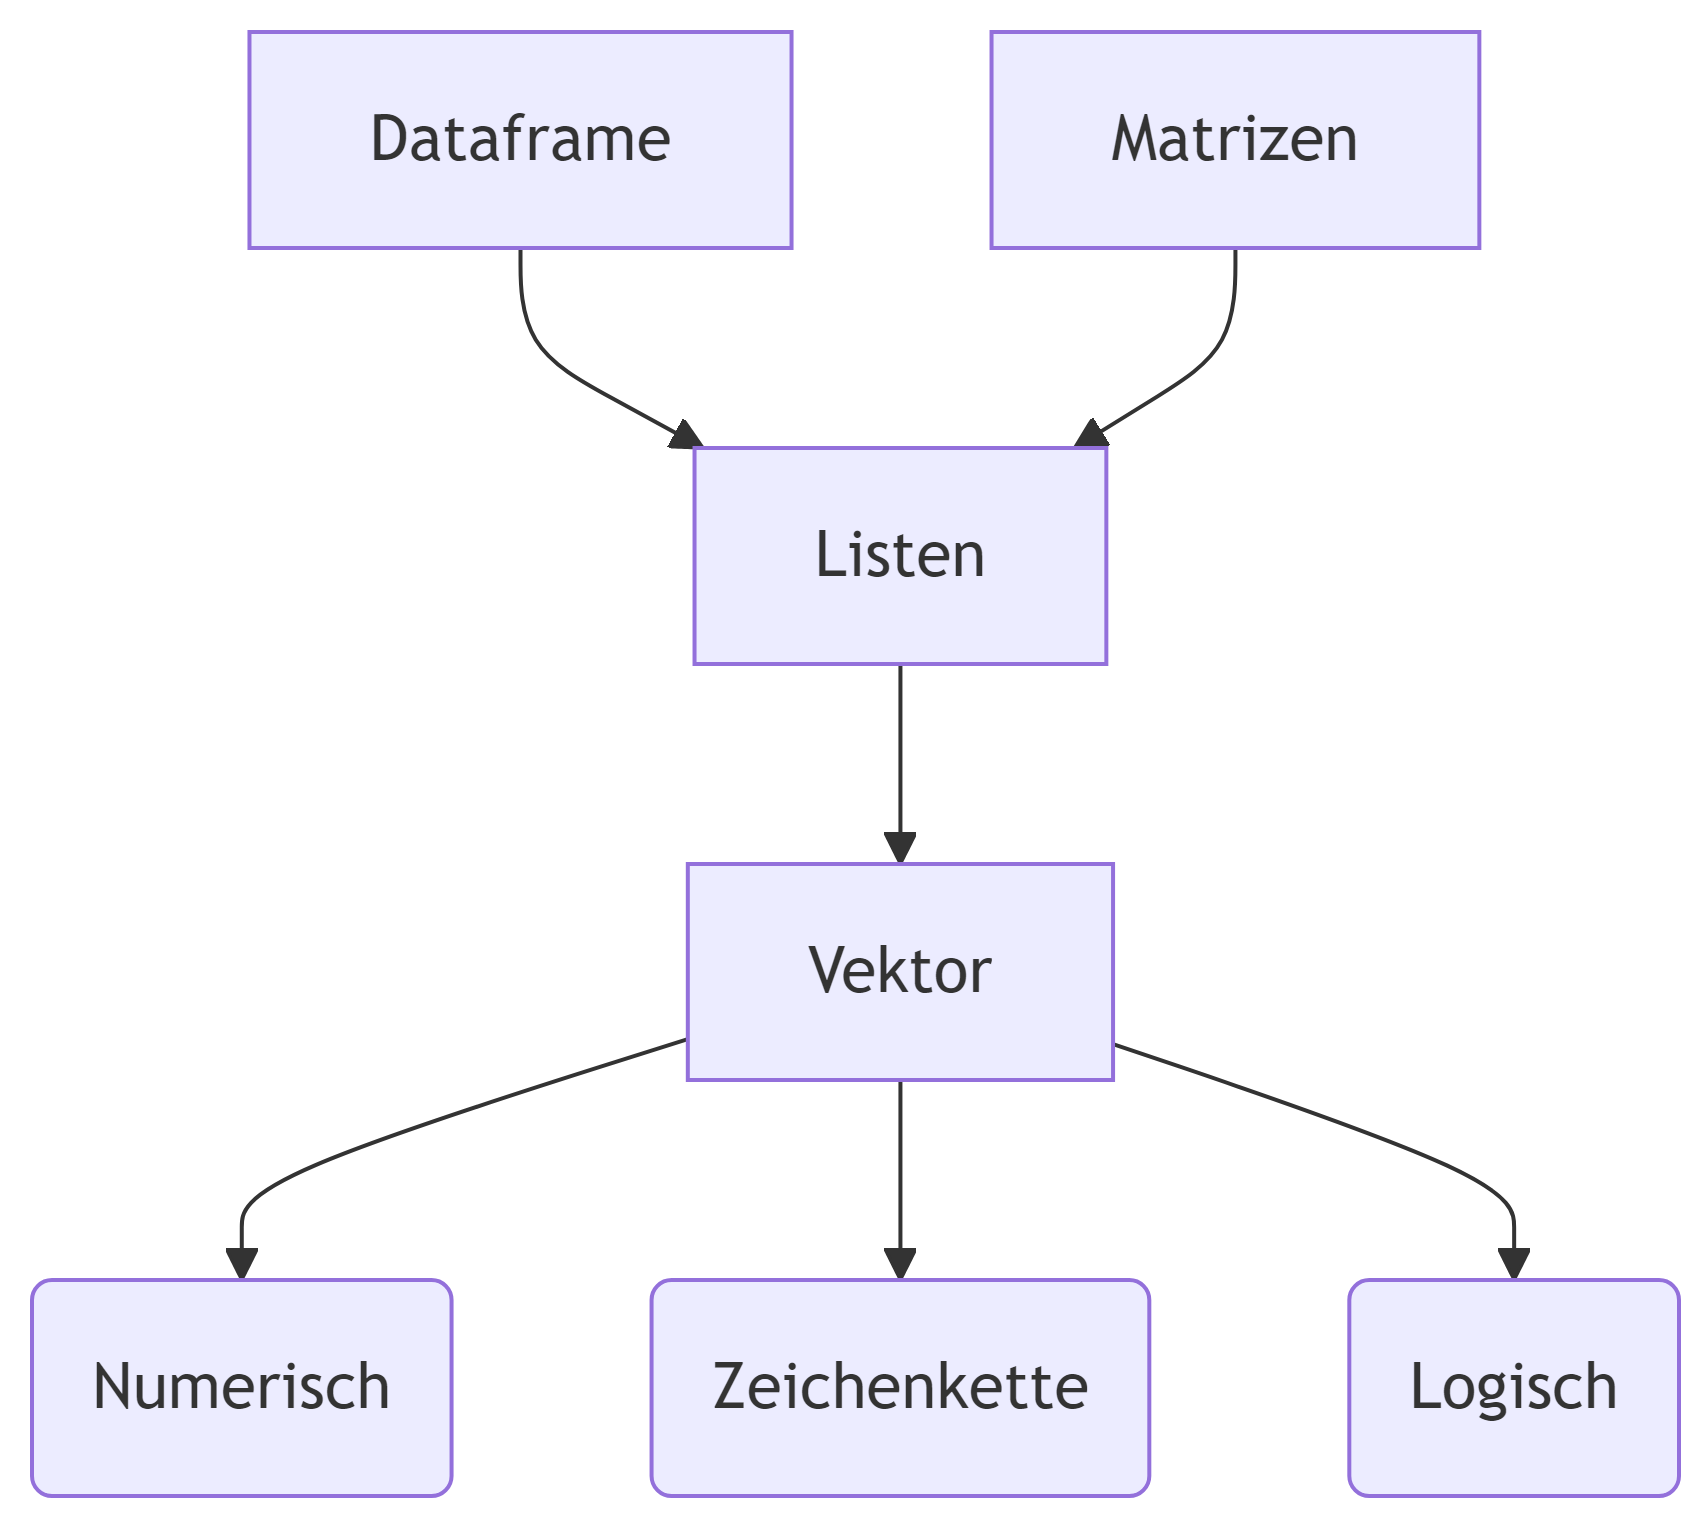
\includegraphics[width=3.99in,height=2.27in]{r_vars_types_files/figure-latex/mermaid-figure-1.png}

}

\caption{\label{fig-r-kickoff-dependencies}Hierarchie der Datentypen.}

\end{figure}%

Dies war natürlich nur eine Übersicht, aber sollte euch schon relativ
weit in der Arbeit mit \texttt{R} bringen.

\chapter{Ablaufkontrolle}\label{ablaufkontrolle}

Nachdem wir die Grunddatentypen in \texttt{R} kennengelernt haben,
schauen wir uns nun drei zentrale Konstrukte der Programmierung an. Das
sind Vergleiche, darauf aufbauend Bedingte Anweisungen und Verzweigungen
und Schleifen. Fangen wir mit den Vergleichen an.

\section{Vergleiche}\label{vergleiche}

Bei Vergleichen wird zunächst einmal genau das gemacht, was im Namen
drinsteht, es werden Sachen miteinander verglichen. Und wenn ich Sachen
schreibe, dann vor allem erst einmal Zahlen. Wenn wir Zahlen miteinander
vergleichen, dann kennen wir die Grundoperatoren noch aus der Schule
(siehe Table~\ref{tbl-comparisons}).

\begin{longtable}[]{@{}ll@{}}
\caption{Vergleichsoperatoren}\label{tbl-comparisons}\tabularnewline
\toprule\noalign{}
Operator & Vergleich \\
\midrule\noalign{}
\endfirsthead
\toprule\noalign{}
Operator & Vergleich \\
\midrule\noalign{}
\endhead
\bottomrule\noalign{}
\endlastfoot
\(<\) & kleiner \\
\(>\) & größer \\
\(<=\) & kleiner oder gleich \\
\(>=\) & größer oder gleich \\
\(==\) & gleich \\
\end{longtable}

Der einzige Vergleichsoperator der etwas ungewohnt erscheinen dürfte ist
der Vergleich auf Gleichheit \texttt{==}. Das einfache
Gleichheitszeichen \texttt{=} ist ähnlich dem Zuweisungsoperator
\texttt{\textless{}-}, daher wird ein weiteres Zeichen verwendet und das
ist eben das doppelte Gleichheitszeichen \texttt{==}. Letztendlich ist
das aber wieder nur Syntax die sich gemerkt werden muss. Wichtiger, in
\texttt{R} ist das Ergebnis eines Vergleichs ein logischer Wert.

\begin{Shaded}
\begin{Highlighting}[]
\SpecialCharTok{\textgreater{}} \DecValTok{3} \SpecialCharTok{\textless{}} \DecValTok{6}
\end{Highlighting}
\end{Shaded}

\begin{verbatim}
[1] TRUE
\end{verbatim}

\begin{Shaded}
\begin{Highlighting}[]
\SpecialCharTok{\textgreater{}} \DecValTok{6} \SpecialCharTok{\textless{}} \DecValTok{3}
\end{Highlighting}
\end{Shaded}

\begin{verbatim}
[1] FALSE
\end{verbatim}

\begin{Shaded}
\begin{Highlighting}[]
\SpecialCharTok{\textgreater{}} \DecValTok{6} \SpecialCharTok{==} \DecValTok{6}
\end{Highlighting}
\end{Shaded}

\begin{verbatim}
[1] TRUE
\end{verbatim}

In allen drei Fällen sehen wir als Ergebnis der Vergleichsausdrücke
einen logischen Wert. Die Vergleichsoperator funktionieren auch mit
Vektoren.

\begin{Shaded}
\begin{Highlighting}[]
\SpecialCharTok{\textgreater{}}\NormalTok{ v\_1 }\OtherTok{\textless{}{-}} \DecValTok{1}\SpecialCharTok{:}\DecValTok{6}
\SpecialCharTok{\textgreater{}}\NormalTok{ v\_2 }\OtherTok{\textless{}{-}} \DecValTok{2}\SpecialCharTok{:}\DecValTok{7}
\SpecialCharTok{\textgreater{}}\NormalTok{ v\_1 }\SpecialCharTok{\textless{}} \DecValTok{3}
\end{Highlighting}
\end{Shaded}

\begin{verbatim}
[1]  TRUE  TRUE FALSE FALSE FALSE FALSE
\end{verbatim}

\begin{Shaded}
\begin{Highlighting}[]
\SpecialCharTok{\textgreater{}} \DecValTok{3} \SpecialCharTok{\textless{}}\NormalTok{ v\_1}
\end{Highlighting}
\end{Shaded}

\begin{verbatim}
[1] FALSE FALSE FALSE  TRUE  TRUE  TRUE
\end{verbatim}

\begin{Shaded}
\begin{Highlighting}[]
\SpecialCharTok{\textgreater{}}\NormalTok{ v\_1 }\SpecialCharTok{\textless{}}\NormalTok{ v\_2}
\end{Highlighting}
\end{Shaded}

\begin{verbatim}
[1] TRUE TRUE TRUE TRUE TRUE TRUE
\end{verbatim}

Wenn beide Objekte Vektoren sind, dann wird der Vergleich Element für
Element durchgeführt, während bei einem Vergleich mit einem Skalar alle
Vektorelemente mit dem Skalar verglichen werden. In beiden Fällen ist
das Ergebnis des Ausdrucks wieder Vektor der entsprechenden Länge mit
logischen Einträgen.

Zusammen mit dem subsetting operator \texttt{{[}{]}} können wir mit
relativ wenig Aufwand Werte die eine bestimmte Bedingung erfüllt aus
einem Vektor extrahieren. Zum Beispiel aus dem Vektor \texttt{v\_1} alle
Werte die kleiner \(4\) sind.

\begin{Shaded}
\begin{Highlighting}[]
\SpecialCharTok{\textgreater{}}\NormalTok{ v\_1[v\_1 }\SpecialCharTok{\textless{}} \DecValTok{4}\NormalTok{]}
\end{Highlighting}
\end{Shaded}

\begin{verbatim}
[1] 1 2 3
\end{verbatim}

Warum hat das funktioniert? Zuerst wird der Vergleich
\texttt{v\_1\ \textless{}\ 4} von \texttt{R} durchgeführt, der
Rückgabewert dieser Operation ist ein Vektor mit logischen Werten
entsprechend des Vergleichs. Der Vektor hat die Länge von \texttt{v\_1},
kann daher direkt dazu benutzt werden Elemente aus \texttt{v\_1} die die
Bedingung erfüllen mit dem subsetting Operator \texttt{{[}{]}} zu
extrahieren.

Da wir logische Wert mit den logischen Operatoren verknüpfen können,
ermöglicht dies auch komplizierte Vergleiche durchzuführe.

\begin{Shaded}
\begin{Highlighting}[]
\SpecialCharTok{\textgreater{}}\NormalTok{ v\_1[v\_1 }\SpecialCharTok{\textless{}} \DecValTok{3} \SpecialCharTok{|}\NormalTok{ v\_1 }\SpecialCharTok{\textgreater{}} \DecValTok{4}\NormalTok{]}
\end{Highlighting}
\end{Shaded}

\begin{verbatim}
[1] 1 2 5 6
\end{verbatim}

\begin{Shaded}
\begin{Highlighting}[]
\SpecialCharTok{\textgreater{}}\NormalTok{ v\_1[v\_1 }\SpecialCharTok{\textgreater{}=} \DecValTok{3} \SpecialCharTok{\&}\NormalTok{ v\_1 }\SpecialCharTok{\textless{}=} \DecValTok{4}\NormalTok{]}
\end{Highlighting}
\end{Shaded}

\begin{verbatim}
[1] 3 4
\end{verbatim}

Die Vergleiche können wir nun verwenden um bedingte Anweisungen zu
verstehen.

\section{Bedingte Anweisungen und
Verzweigungen}\label{bedingte-anweisungen-und-verzweigungen}

In Figure~\ref{fig-r-flow-ifelse} ist der Grundgerüst einer bedingten
Anweisungen bzw. Verzweigung im Code dargestellt.

\begin{figure}

\centering{

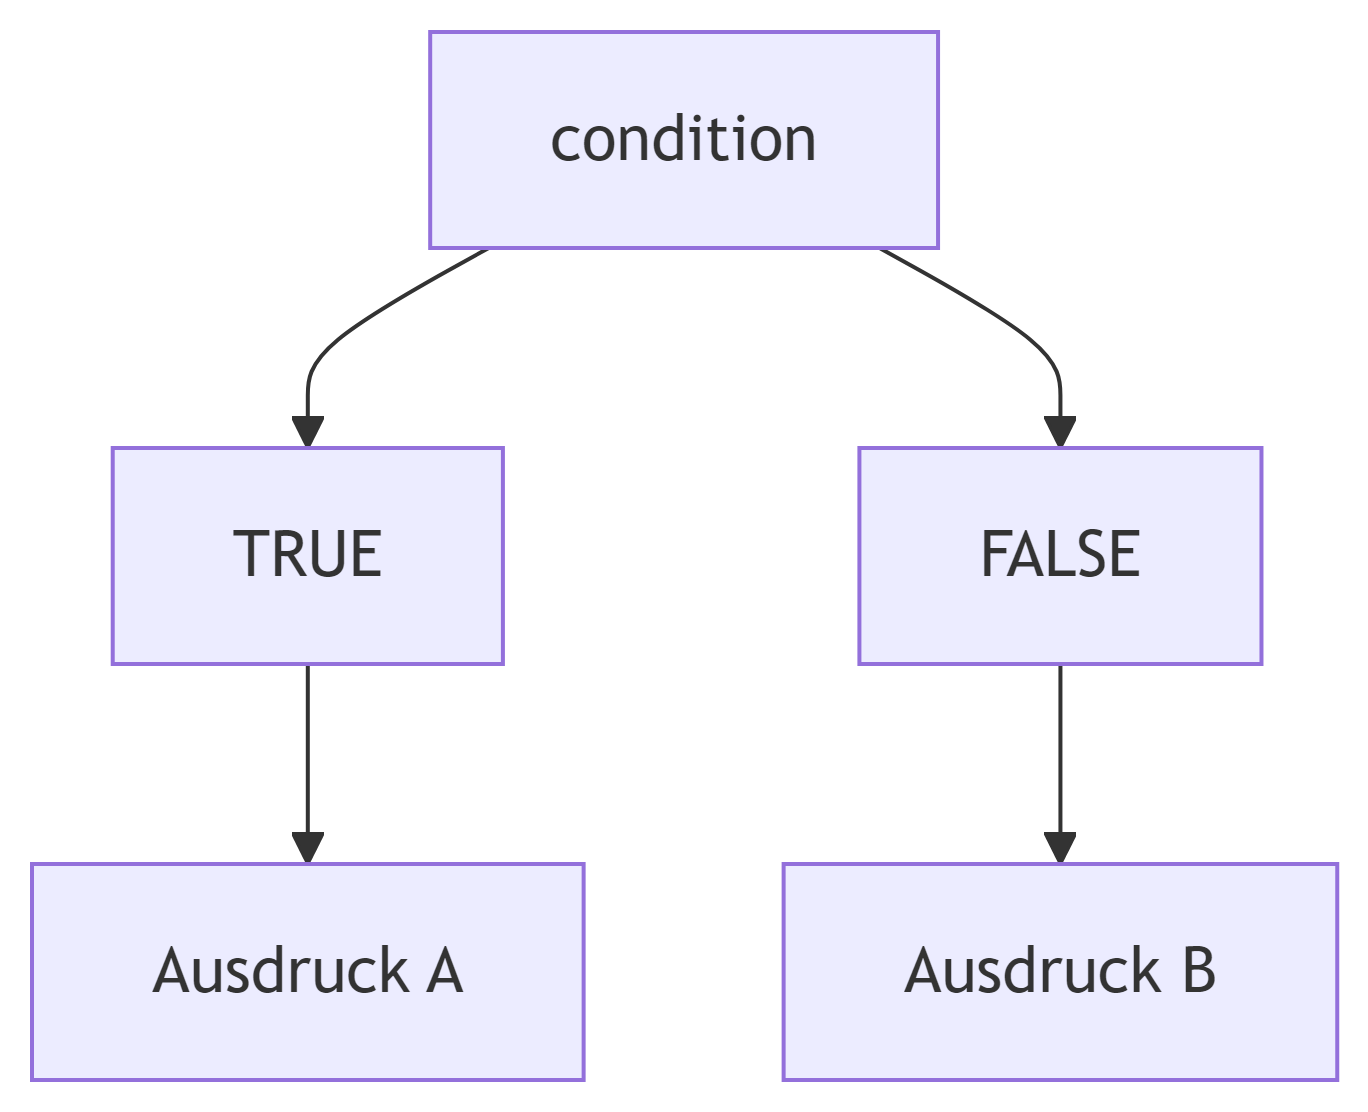
\includegraphics[width=2.63in,height=2.27in]{r_flowcontrol_files/figure-latex/mermaid-figure-1.png}

}

\caption{\label{fig-r-flow-ifelse}Bedingte Anweisungen.}

\end{figure}%

Wir haben einen Ausdruck \texttt{condition} der entweder \texttt{WAHR}
oder \texttt{FALSCH} sein kann, und entsprechend wird entweder
\texttt{Ausdruck\ A} oder \texttt{Ausdruck\ B} ausgeführt. In
\texttt{condition} wird überlicherweise in irgendeiner Form ein
Vergleich vorgenommen.

Syntaktisch wird die Bedingte Anweisung in \texttt{R} folgendermaßen
spezifiziert.

\phantomsection\label{annotated-cell-137}%
\begin{Shaded}
\begin{Highlighting}[]
\SpecialCharTok{\textgreater{}} \ControlFlowTok{if}\NormalTok{ (condition) \{ }\hspace*{\fill}\NormalTok{\circled{1}}
\SpecialCharTok{+}\NormalTok{   AusdruckA }\hspace*{\fill}\NormalTok{\circled{2}}
\SpecialCharTok{+}\NormalTok{ \} }\ControlFlowTok{else}\NormalTok{ \{         }\CommentTok{\# }
\SpecialCharTok{+}\NormalTok{   AusdruckB }\hspace*{\fill}\NormalTok{\circled{3}}
\SpecialCharTok{+}\NormalTok{ \}}
\end{Highlighting}
\end{Shaded}

\begin{description}
\tightlist
\item[\circled{1}]
Zunächst kommt das Schlüsselwort \texttt{if} gefolgt von einer Klammer
mit dem Ausdruck \texttt{condition} der zu einem logischen Wert
(\texttt{true,false}) evaluiert wird.
\item[\circled{2}]
Wenn \texttt{condition} \texttt{TRUE} ist, wird der \texttt{AusdruckA}
innerhalb der geschweiften Klammern ausgeführt.
\item[\circled{3}]
Wenn \texttt{condition} \texttt{FALSE} ist, wird der \texttt{else}
Zweig, bzw. der \texttt{AusdruckB} zwischen den geschweiften Klammern
nach \texttt{else} ausgeführt.
\end{description}

Schauen wir uns ein einfaches Beispiel an:

\begin{Shaded}
\begin{Highlighting}[]
\SpecialCharTok{\textgreater{}}\NormalTok{ m }\OtherTok{\textless{}{-}} \DecValTok{0}
\SpecialCharTok{\textgreater{}}\NormalTok{ a }\OtherTok{\textless{}{-}} \DecValTok{10}
\SpecialCharTok{\textgreater{}}\NormalTok{ b }\OtherTok{\textless{}{-}} \DecValTok{20}
\SpecialCharTok{\textgreater{}} \ControlFlowTok{if}\NormalTok{ (a }\SpecialCharTok{\textless{}}\NormalTok{ b) \{}
\SpecialCharTok{+}\NormalTok{   m }\OtherTok{\textless{}{-}} \DecValTok{10}
\SpecialCharTok{+}\NormalTok{ \} }\ControlFlowTok{else}\NormalTok{ \{}
\SpecialCharTok{+}\NormalTok{   m }\OtherTok{\textless{}{-}} \DecValTok{20}
\SpecialCharTok{+}\NormalTok{ \}}
\SpecialCharTok{\textgreater{}}\NormalTok{ m}
\end{Highlighting}
\end{Shaded}

\begin{verbatim}
[1] 10
\end{verbatim}

Was passiert hier, der Wert von \texttt{m} wird unterschiedlich belegt,
je nachdem welche Werte \texttt{a} und \texttt{b} haben. Mit diesem
\texttt{ifelse}-Konstrukt können wir daher unterschiedliche Anweisungen
in unseren Programmen ausführen lassen, in Abhängigkeit von bestimmten
Bedingungen. Wir könnten zum Beispiel unsere eigene Absolutfunktion
schreiben.

\begin{Shaded}
\begin{Highlighting}[]
\SpecialCharTok{\textgreater{}}\NormalTok{ my\_abs }\OtherTok{\textless{}{-}} \ControlFlowTok{function}\NormalTok{(x) \{}
\SpecialCharTok{+}   \ControlFlowTok{if}\NormalTok{ (x }\SpecialCharTok{\textless{}} \DecValTok{0}\NormalTok{) \{}
\SpecialCharTok{+}     \SpecialCharTok{{-}}\NormalTok{x}
\SpecialCharTok{+}\NormalTok{   \} }\ControlFlowTok{else}\NormalTok{ \{}
\SpecialCharTok{+}\NormalTok{     x}
\SpecialCharTok{+}\NormalTok{   \}}
\SpecialCharTok{+}\NormalTok{ \}}
\SpecialCharTok{\textgreater{}} \FunctionTok{my\_abs}\NormalTok{(}\DecValTok{3}\NormalTok{)}
\end{Highlighting}
\end{Shaded}

\begin{verbatim}
[1] 3
\end{verbatim}

\begin{Shaded}
\begin{Highlighting}[]
\SpecialCharTok{\textgreater{}} \FunctionTok{my\_abs}\NormalTok{(}\DecValTok{0}\NormalTok{)}
\end{Highlighting}
\end{Shaded}

\begin{verbatim}
[1] 0
\end{verbatim}

\begin{Shaded}
\begin{Highlighting}[]
\SpecialCharTok{\textgreater{}} \FunctionTok{my\_abs}\NormalTok{(}\SpecialCharTok{{-}}\DecValTok{3}\NormalTok{)}
\end{Highlighting}
\end{Shaded}

\begin{verbatim}
[1] 3
\end{verbatim}

\section{\texorpdfstring{\texttt{for}-Schleifen}{for-Schleifen}}\label{for-schleifen}

Als letztes Programmierkonstrukt kommen jetzt noch Schleifen, eine der
Paradedisziplin von Computern, nämlich die gleiche Sache ganz oft
hintereinander durchführen.

Die Syntax für eine Schleife in \texttt{R} ist wie folgt.

\phantomsection\label{annotated-cell-142}%
\begin{Shaded}
\begin{Highlighting}[]
\SpecialCharTok{\textgreater{}} \ControlFlowTok{for}\NormalTok{ (item }\ControlFlowTok{in}\NormalTok{ vector) \{ }\hspace*{\fill}\NormalTok{\circled{1}}
\SpecialCharTok{+}\NormalTok{   Ausdruck }\hspace*{\fill}\NormalTok{\circled{2}}
\SpecialCharTok{+}\NormalTok{ \}}
\end{Highlighting}
\end{Shaded}

\begin{description}
\tightlist
\item[\circled{1}]
Als erstes kommt das Schlüsselwort \texttt{for} gefolgt von einer
Klammer. In der Klammer werden zwei Ausdrücke benötigt. Eine Variable
die hier \texttt{item} heißt, die als Schleifenzähler fungiert. Der
Schleifenzähler durchläuft die Einträge des Vektors \texttt{vector}
einen nach dem anderen.
\item[\circled{2}]
Jedes Mal wenn \texttt{item} mit einem neuen Wert belegt worden ist,
wird \texttt{Ausdruck} zwischen den geschweiften Klammer \texttt{\{\}}
ausgeführt. Der jeweilige aktuelle Wert von \texttt{item} steht im
Ausdruck zur Verfügung.
\end{description}

Hört sich komplizierter an als es ist. Ein einfaches Beispiel:

\begin{Shaded}
\begin{Highlighting}[]
\SpecialCharTok{\textgreater{}} \ControlFlowTok{for}\NormalTok{ (i }\ControlFlowTok{in} \DecValTok{1}\SpecialCharTok{:}\DecValTok{4}\NormalTok{) \{}
\SpecialCharTok{+}   \FunctionTok{cat}\NormalTok{(}\StringTok{\textquotesingle{}Ausdruck wird ausgeführt}\SpecialCharTok{\textbackslash{}n}\StringTok{\textquotesingle{}}\NormalTok{)}
\SpecialCharTok{+}   \FunctionTok{cat}\NormalTok{(}\StringTok{\textquotesingle{}i =\textquotesingle{}}\NormalTok{, i, }\StringTok{\textquotesingle{}}\SpecialCharTok{\textbackslash{}n}\StringTok{\textquotesingle{}}\NormalTok{)}
\SpecialCharTok{+}\NormalTok{ \}}
\end{Highlighting}
\end{Shaded}

\begin{verbatim}
Ausdruck wird ausgeführt
i = 1 
Ausdruck wird ausgeführt
i = 2 
Ausdruck wird ausgeführt
i = 3 
Ausdruck wird ausgeführt
i = 4 
\end{verbatim}

Wir verwenden in dem Code die \texttt{cat()} Funktion um die Wert auf
der Kommandozeile auszugeben. Das Zeichen \texttt{\textbackslash{}n} ist
lediglich ein Sonderzeichen für neue Zeile. Was passiert in dem Code.
Wir haben einen Vektor mit den Elementen von \(1,2,3,4\). Die Variable
\texttt{item} hat jetzt den Namen \texttt{i}. \texttt{i} wird Element
für Element mit den Einträgen aus dem Vektor belegt und jedes mal wird
der Ausdruck zwischen den Klammern ausgeführt.

Ein wird könnten nun zum Beispiel den Vektor als Index für die Einträge
in einen anderen Vektor mit Elementen ansehen und dementsprechend über
die Einträge des anderen Vektoren mit \texttt{i} iterieren.

\begin{Shaded}
\begin{Highlighting}[]
\SpecialCharTok{\textgreater{}}\NormalTok{ vec }\OtherTok{\textless{}{-}} \FunctionTok{c}\NormalTok{(}\StringTok{\textquotesingle{}mama\textquotesingle{}}\NormalTok{,}\StringTok{\textquotesingle{}papa\textquotesingle{}}\NormalTok{,}\StringTok{\textquotesingle{}daughter\textquotesingle{}}\NormalTok{,}\StringTok{\textquotesingle{}son\textquotesingle{}}\NormalTok{) }
\SpecialCharTok{\textgreater{}} \ControlFlowTok{for}\NormalTok{ (i }\ControlFlowTok{in} \DecValTok{1}\SpecialCharTok{:}\DecValTok{4}\NormalTok{) \{}
\SpecialCharTok{+}   \FunctionTok{cat}\NormalTok{(}\StringTok{\textquotesingle{}Ausdruck wird ausgeführt}\SpecialCharTok{\textbackslash{}n}\StringTok{\textquotesingle{}}\NormalTok{)}
\SpecialCharTok{+}   \FunctionTok{cat}\NormalTok{(}\StringTok{\textquotesingle{}i =\textquotesingle{}}\NormalTok{, i, }\StringTok{\textquotesingle{}: \textquotesingle{}}\NormalTok{, vec[i], }\StringTok{\textquotesingle{}}\SpecialCharTok{\textbackslash{}n}\StringTok{\textquotesingle{}}\NormalTok{)}
\SpecialCharTok{+}\NormalTok{ \}}
\end{Highlighting}
\end{Shaded}

\begin{verbatim}
Ausdruck wird ausgeführt
i = 1 :  mama 
Ausdruck wird ausgeführt
i = 2 :  papa 
Ausdruck wird ausgeführt
i = 3 :  daughter 
Ausdruck wird ausgeführt
i = 4 :  son 
\end{verbatim}

\subsection{\texorpdfstring{Ein längeres Beispiel mit
\texttt{for}}{Ein längeres Beispiel mit for}}\label{ein-luxe4ngeres-beispiel-mit-for}

Zum Abschluss schauen wir uns ein Beispiel aus der Statistik an zu
Publikationsfilter und welche Auswirkung der Filter auf die Effektstärke
hat.

Wir machen führen wiederholte t-Tests aus. Wir gehen davon aus, dass es
eine Effektstärke von \(D = 0.1\) gibt. Dazu ziehen wir zwei Stichproben
der Größe \(n\) aus den entsprechenden Normalverteilung die unserer
Populationen darstellen. Dann berechnen wir den t-Test und wenn es sich
um ein statistisch signifikantes Ergebnis handelt dann speichern wir den
Unterschied zwischen den beiden Gruppen. Da es sich um ein
Zufallsexperiment handelt, wissen wir vorher nicht, wie viele Vergleiche
statistisch signifikant werden und wir speichern müssen, daher erstellen
wir einen Ergebnisvektor der gleichen Länge wie oft wir das Experiment
durchführen. Wir setzen der Einfachheit halber
\(n = 10, \delta = 0.1, \sigma = 1, \alpha = 0.05\) (zweiseitig).
Dadurch ist der Unterschied zwischen den beiden Stichproben auch direkt
als Cohen's D Effektstärke zu interpretieren. Führen wir die Simulation
\(N_{sim} = 100\) durch. Mit der Funktion \texttt{rnorm()} können wir
normalverteilte Zufallszahlen ziehen und mit \texttt{qt()} können wir
den kritischen Wert der t-Verteilung bestimmen. In Code:

\begin{Shaded}
\begin{Highlighting}[]
\SpecialCharTok{\textgreater{}}\NormalTok{ n\_sim }\OtherTok{\textless{}{-}} \DecValTok{100}
\SpecialCharTok{\textgreater{}}\NormalTok{ n }\OtherTok{\textless{}{-}} \DecValTok{10}
\SpecialCharTok{\textgreater{}}\NormalTok{ mu }\OtherTok{\textless{}{-}} \DecValTok{0}
\SpecialCharTok{\textgreater{}}\NormalTok{ delta }\OtherTok{\textless{}{-}} \FloatTok{0.1}
\SpecialCharTok{\textgreater{}}\NormalTok{ sigma }\OtherTok{\textless{}{-}} \DecValTok{1}
\SpecialCharTok{\textgreater{}}\NormalTok{ df }\OtherTok{\textless{}{-}} \DecValTok{2}\SpecialCharTok{*}\NormalTok{n }\SpecialCharTok{{-}} \DecValTok{2}
\SpecialCharTok{\textgreater{}}\NormalTok{ kritischer\_wert }\OtherTok{\textless{}{-}} \FunctionTok{qt}\NormalTok{(}\FloatTok{0.975}\NormalTok{, df)}
\SpecialCharTok{\textgreater{}}\NormalTok{ ergebnis\_vektor }\OtherTok{\textless{}{-}} \FunctionTok{numeric}\NormalTok{(n\_sim)}
\SpecialCharTok{\textgreater{}} \ControlFlowTok{for}\NormalTok{ (i }\ControlFlowTok{in} \DecValTok{1}\SpecialCharTok{:}\NormalTok{n\_sim) \{}
\SpecialCharTok{+}   \CommentTok{\# ziehen der Stichproben}
\SpecialCharTok{+}\NormalTok{   stichprobe\_a }\OtherTok{\textless{}{-}} \FunctionTok{rnorm}\NormalTok{(n, mu, sigma)}
\SpecialCharTok{+}\NormalTok{   stichprobe\_b }\OtherTok{\textless{}{-}} \FunctionTok{rnorm}\NormalTok{(n, delta, sigma)}
\SpecialCharTok{+}   
\SpecialCharTok{+}   \CommentTok{\# zwischenwerte berechnen}
\SpecialCharTok{+}\NormalTok{   a\_bar }\OtherTok{\textless{}{-}} \FunctionTok{mean}\NormalTok{(stichprobe\_a)}
\SpecialCharTok{+}\NormalTok{   b\_bar }\OtherTok{\textless{}{-}} \FunctionTok{mean}\NormalTok{(stichprobe\_b)}
\SpecialCharTok{+}\NormalTok{   a\_sd }\OtherTok{\textless{}{-}} \FunctionTok{sd}\NormalTok{(stichprobe\_a)}
\SpecialCharTok{+}\NormalTok{   b\_sd }\OtherTok{\textless{}{-}} \FunctionTok{sd}\NormalTok{(stichprobe\_b)}
\SpecialCharTok{+}   
\SpecialCharTok{+}   \CommentTok{\# t{-}Statistik berechnen}
\SpecialCharTok{+}\NormalTok{   Delta }\OtherTok{\textless{}{-}} \FunctionTok{abs}\NormalTok{(a\_bar }\SpecialCharTok{{-}}\NormalTok{ b\_bar)}
\SpecialCharTok{+}\NormalTok{   s\_pooled }\OtherTok{\textless{}{-}} \FunctionTok{sqrt}\NormalTok{((a\_sd}\SpecialCharTok{**}\DecValTok{2} \SpecialCharTok{+}\NormalTok{ b\_sd}\SpecialCharTok{**}\DecValTok{2}\NormalTok{)}\SpecialCharTok{/}\DecValTok{2}\NormalTok{)}
\SpecialCharTok{+}\NormalTok{   s\_e }\OtherTok{\textless{}{-}}\NormalTok{ s\_pooled }\SpecialCharTok{*} \FunctionTok{sqrt}\NormalTok{(}\DecValTok{2}\SpecialCharTok{/}\NormalTok{n)}
\SpecialCharTok{+}\NormalTok{   t }\OtherTok{\textless{}{-}}\NormalTok{ Delta}\SpecialCharTok{/}\NormalTok{s\_e}
\SpecialCharTok{+}   
\SpecialCharTok{+}   \CommentTok{\# überprüfen auf statistische Signifikanz}
\SpecialCharTok{+}   \ControlFlowTok{if}\NormalTok{ (t }\SpecialCharTok{\textgreater{}}\NormalTok{ kritischer\_wert) \{}
\SpecialCharTok{+}\NormalTok{     ergebnis\_vektor[i] }\OtherTok{\textless{}{-}}\NormalTok{ Delta}
\SpecialCharTok{+}\NormalTok{   \}}
\SpecialCharTok{+}\NormalTok{ \}}
\SpecialCharTok{\textgreater{}} 
\ErrorTok{\textgreater{}}\NormalTok{ statistisch\_signifikant }\OtherTok{\textless{}{-}}\NormalTok{ ergebnis\_vektor[ergebnis\_vektor }\SpecialCharTok{\textgreater{}} \DecValTok{0}\NormalTok{]}
\SpecialCharTok{\textgreater{}}\NormalTok{ D\_bar }\OtherTok{\textless{}{-}} \FunctionTok{mean}\NormalTok{(statistisch\_signifikant)}
\SpecialCharTok{\textgreater{}}\NormalTok{ D\_sd }\OtherTok{\textless{}{-}} \FunctionTok{sd}\NormalTok{(statistisch\_signifikant)}
\SpecialCharTok{\textgreater{}} \FunctionTok{cat}\NormalTok{(}\StringTok{\textquotesingle{}Die Effektstärke ist D =\textquotesingle{}}\NormalTok{, D\_bar,}\StringTok{\textquotesingle{}+{-}\textquotesingle{}}\NormalTok{, D\_sd, }\StringTok{\textquotesingle{}}\SpecialCharTok{\textbackslash{}n}\StringTok{\textquotesingle{}}\NormalTok{)}
\end{Highlighting}
\end{Shaded}

\begin{verbatim}
Die Effektstärke ist D = 1.010578 +- 0.3888277 
\end{verbatim}

Als Hausaufgaben versucht das Programm nachzuvollziehen und das Ergebnis
zu interpretieren.

\section{\texorpdfstring{Wiederholungen mit
\texttt{replicate()}}{Wiederholungen mit replicate()}}\label{wiederholungen-mit-replicate}

Eine weitere Möglichkeit \texttt{R} eine Gruppe von Anweisungen
wiederholt durchführen zu lassen, kann mittels der Funktion
\texttt{replicate()} erreicht werden. In den meisten Fällen wird
\texttt{replicate()} verwendet um eine Simulation durchzuführen. D.h.
das Beispiel von eben könnte ebenfalls mittels \texttt{replicate()}
programmiert werden. \texttt{replicate()} hat zwei Hauptargumente. Das
erste \texttt{n} bestimmt die Anzahl der Wiederholungen während das
zweite Argument eine Anweisung, in den meisten Fällen eine Funktion ist.

Nehmen wir als Anwendungsfall, dass wir wiederholt Mittelwerte
\(\bar{x}\) aus einer Zufallsstichprobe erzeugen wollen. Wir ziehen
beispielsweise eine Stichprobe von \(n = 20\) Werten aus einer
Normalverteilung mit den Parametern \(\mu = 3, \sigma = .7\). Und wir
wollen uns die Stichprobenverteilung der Mittelwerte ansehen. Wir
beginnen mit einem einfach proof-of-concept.

\begin{Shaded}
\begin{Highlighting}[]
\SpecialCharTok{\textgreater{}}\NormalTok{ mu }\OtherTok{\textless{}{-}} \DecValTok{3}
\SpecialCharTok{\textgreater{}}\NormalTok{ sigma }\OtherTok{\textless{}{-}} \FloatTok{0.7}
\SpecialCharTok{\textgreater{}}\NormalTok{ n }\OtherTok{\textless{}{-}} \DecValTok{20}
\SpecialCharTok{\textgreater{}} 
\ErrorTok{\textgreater{}}\NormalTok{ x\_bar }\OtherTok{\textless{}{-}} \FunctionTok{mean}\NormalTok{(}\FunctionTok{rnorm}\NormalTok{(n, mu, sigma))}
\SpecialCharTok{\textgreater{}} \FunctionTok{cat}\NormalTok{(}\StringTok{\textquotesingle{}Der beobachtete Mittelwert ist: \textquotesingle{}}\NormalTok{, x\_bar, }\StringTok{\textquotesingle{}}\SpecialCharTok{\textbackslash{}n}\StringTok{\textquotesingle{}}\NormalTok{)}
\end{Highlighting}
\end{Shaded}

\begin{verbatim}
Der beobachtete Mittelwert ist:  3.110733 
\end{verbatim}

Okay, funktioniert. Wir wollen diese Anweisung jetzt nicht einmal
sondern \(100\)mal durchführen. Dazu stecken wir sie in eine Funktion
(streng genommen brauchen wir das nicht, aber damit es besser
generalisiert machen wir hier etwas mehr Aufwand). Die Parameter für die
Normalverteilung setzen wir in der Signatur der Funktion als
Standardwerte.

\begin{Shaded}
\begin{Highlighting}[]
\SpecialCharTok{\textgreater{}}\NormalTok{ x\_bar\_func }\OtherTok{\textless{}{-}} \ControlFlowTok{function}\NormalTok{(}\AttributeTok{n =} \DecValTok{20}\NormalTok{, }\AttributeTok{mu =} \DecValTok{3}\NormalTok{, }\AttributeTok{sigma =} \FloatTok{0.7}\NormalTok{) \{}
\SpecialCharTok{+}   \FunctionTok{mean}\NormalTok{(}\FunctionTok{rnorm}\NormalTok{(n, mu, sigma))}
\SpecialCharTok{+}\NormalTok{ \}}
\end{Highlighting}
\end{Shaded}

Wenn wir \texttt{x\_bar\_func()} aufrufen, erhalten wir entsprechend
einen zufälligen Mittelwert aus einer Stichrprobe der Größe \(n = 20\)
aus der Normalverteilung \(\mathcal{N}(3, 0.7)\).

\begin{Shaded}
\begin{Highlighting}[]
\SpecialCharTok{\textgreater{}} \FunctionTok{x\_bar\_func}\NormalTok{()}
\end{Highlighting}
\end{Shaded}

\begin{verbatim}
[1] 2.839709
\end{verbatim}

Diese Funktion können wir nun an \texttt{replicate()} als zweiters
Argument übergeben mit dem ersten Argument der Anzahl der
Wiederholungen. Starten wir erst mal nur mit \(N_{sim} = 5\)
Wiederholungen, um den Überblick zu behalten.

\begin{Shaded}
\begin{Highlighting}[]
\SpecialCharTok{\textgreater{}}\NormalTok{ N\_sim }\OtherTok{\textless{}{-}} \DecValTok{5}
\SpecialCharTok{\textgreater{}} \FunctionTok{replicate}\NormalTok{(N\_sim, }\FunctionTok{x\_bar\_func}\NormalTok{())}
\end{Highlighting}
\end{Shaded}

\begin{verbatim}
[1] 2.908909 3.089300 2.949479 2.750709 2.831800
\end{verbatim}

Als Rückgabewert von \texttt{x\_bar\_func()} erhalten wir einen Vektor
mit den Rückgabewerten von \texttt{x\_bar\_func()}. Dementsprechend
können wir den Rückgabewert an eine Variable zuweisen und können uns zum
Beispiel ein Histogramm der Mittelwert erzeugen.

\begin{Shaded}
\begin{Highlighting}[]
\SpecialCharTok{\textgreater{}}\NormalTok{ N\_sim }\OtherTok{\textless{}{-}} \DecValTok{100}
\SpecialCharTok{\textgreater{}}\NormalTok{ x\_bar\_s }\OtherTok{\textless{}{-}} \FunctionTok{replicate}\NormalTok{(N\_sim, }\FunctionTok{x\_bar\_func}\NormalTok{())}
\SpecialCharTok{\textgreater{}} \FunctionTok{hist}\NormalTok{(x\_bar\_s)}
\end{Highlighting}
\end{Shaded}

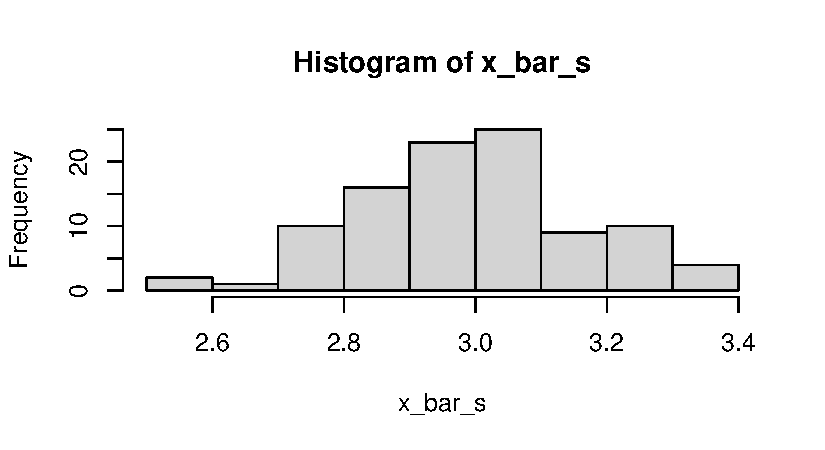
\includegraphics{r_flowcontrol_files/figure-pdf/unnamed-chunk-18-1.pdf}

Zusammenfassend, beginnen wir mit der Definition einer Funktion welche
die benötigten Werte erzeugt. Diese Funktion übergeben wir an
\texttt{replicate()} und können so einfach bestimmte Werte generieren.

Der Vollständigkeit halber eine Ausführung mit einer
\texttt{for}-Schleife.

\begin{Shaded}
\begin{Highlighting}[]
\SpecialCharTok{\textgreater{}}\NormalTok{ x\_bar\_s2 }\OtherTok{\textless{}{-}} \FunctionTok{numeric}\NormalTok{(N\_sim)}
\SpecialCharTok{\textgreater{}} \ControlFlowTok{for}\NormalTok{ (i }\ControlFlowTok{in} \DecValTok{1}\SpecialCharTok{:}\NormalTok{N\_sim) \{}
\SpecialCharTok{+}\NormalTok{   x\_bar\_s2[i] }\OtherTok{\textless{}{-}} \FunctionTok{x\_bar\_func}\NormalTok{()}
\SpecialCharTok{+}\NormalTok{ \}}
\SpecialCharTok{\textgreater{}} \FunctionTok{hist}\NormalTok{(x\_bar\_s2)}
\end{Highlighting}
\end{Shaded}

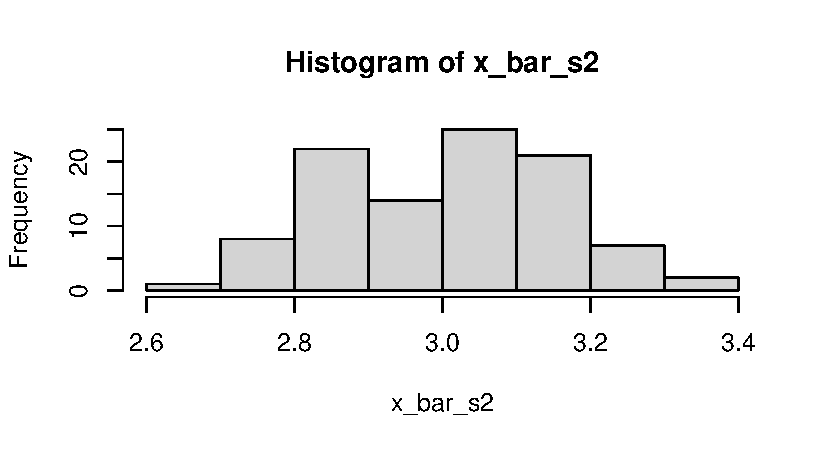
\includegraphics{r_flowcontrol_files/figure-pdf/unnamed-chunk-19-1.pdf}

Hier sehen wir, dass der Code nicht viel länger ist, wir aber expliziter
uns um die Zuweisung der Ergebnisse kümmern müssen, während dies bei
\texttt{replicate()} automatisch stattfindet. D.h. wenn wir mit der
Schleifenvariable nichts explizit machen müssen/wollen, dann bietet
\texttt{replicate()} eine Alternative zu \texttt{for}-Schleifen.

\chapter{\texorpdfstring{Eigene Funktionen in
\texttt{R}}{Eigene Funktionen in R}}\label{eigene-funktionen-in-r}

Eine zentrale Tätigkeit im Umgang mit jeder Programmiersprache ist das
schreiben von eigenen Funktionen. Es ist zwar möglich relativ weit zu
kommen ohne eigene Funktionen zu schreiben aber es ergeben sich um
Umgang mit Daten immer wieder Situationen in denen immer wieder die
gleichen Schritte durchgeführt werden. Dies führt dann oft zu
copy-and-paste von Anweisungen. In solchen Fällen ist es oft hilfreich
in der Lage zu sein eigene Funktionen schreiben zu können. Funktionen
bieten hierdurch die Möglichkeit den eigenen Code in verschiedene
logische Einheiten zu strukturieren und dadurch leichter lesbar und
robuster zu machen. Letztendlich beruht der große Erfolg von \texttt{R}
darauf durch eigene Funktionen die Funktionalität von \texttt{R} ständig
erweitern zu können. Daher ist ein zumindest rudimentäres Verständnis
der Semantik von Funktionen in \texttt{R} enorm hilfreich.

Ein erstes, hilfreiches mentales Template für Funktionen in
Programmiersprachen sind Funktionen wie wir sie in der Mathematik
kennengelernt haben.

\begin{equation*}
y = f(x)
\end{equation*}

Wir haben eine Funktion \(f()\), dieser Funktion \(f()\) übergeben wir
ein Argument (auch Parameter genannt) \(x\). Die Funktion \(f()\) macht
dann etwas mit diesem Parameter und gibt einen Rückgabewert zurück, den
wir einer neuen Variable \(y\) zuweisen. Sei zum Beispiel die folgenden
Funktion definiert.

\begin{equation*}
f(x) = x^2
\end{equation*}

D.h. der Funktion \(f()\) wird der Parameter \(x\) übergeben. Dieser
Wert wird anschließend quadriert und das Ergebnis der Berechnung wird
zurück gegeben.

In \texttt{R} werden Funktionen nach dem Muster (,,\ldots,) aufgerufen
(die Zeichen \textless\textgreater{} stehen für einen beliebigen
Bezeichner). D.h. sobald ein rundes Klammerpaar auf einen Bezeichner
folgt, geht \texttt{R} davon aus, dass die Anwenderin eine Funktion
aufrufen möchte. Über ,,\ldots, können der Funktion durch Komma
getrennte Parameter übergeben werden. Die Anzahl der Parameter hängt
dabei von der Definition der Funktion ab. In der Mathematik wäre ein
Beispiel eine Funktion mit zwei Argumenten.

\begin{equation*}
f(x,y) = x^2 + y^2
\end{equation*}

\section{Funktionen anwenden}\label{funktionen-anwenden-1}

Ein einfaches Beispiel ist die Anwendung der Wurzelfunktion auf einen
numerischen Wert. In \texttt{R} gibt es schon eine vordefinierte
Funktion mit dem Bezeichner \texttt{sqrt()}, welche die Wurzel des
übergebenen Parameters berechnet.

\begin{Shaded}
\begin{Highlighting}[]
\SpecialCharTok{\textgreater{}}\NormalTok{ y }\OtherTok{\textless{}{-}} \DecValTok{9}
\SpecialCharTok{\textgreater{}} \FunctionTok{sqrt}\NormalTok{(y)}
\end{Highlighting}
\end{Shaded}

\begin{verbatim}
[1] 3
\end{verbatim}

Im Beispiel wird zunächst dem Wert \(9\) der Bezeichner \texttt{y}
zugewiesen. Dieser wird dann an die Wurzelfunktion \texttt{sqrt()}
übergeben.

Ein etwas näher an der Anwendung liegendes Beispiel wäre beispielsweise
die Berechnung des Mittelwerts oder die Summe der Datenreihe
\((3, 5, 7)\) sein. In \texttt{R} wird eine solche geordnete Reihe von
Zahlen als Vektor repräsentiert. Um einen solchen Vektor zu erstellen
wird wiederum eine Funktion \texttt{c()} (für concatenation) verwendet.

\begin{Shaded}
\begin{Highlighting}[]
\SpecialCharTok{\textgreater{}}\NormalTok{ z }\OtherTok{\textless{}{-}} \FunctionTok{c}\NormalTok{(}\DecValTok{3}\NormalTok{, }\DecValTok{5}\NormalTok{, }\DecValTok{7}\NormalTok{)}
\end{Highlighting}
\end{Shaded}

Mit dieser Anweisung hat \texttt{R} einen Vektor mit den drei Einträgen
erstellt. Wir können jetzt den Mittelwert
\(\bar{z} = \frac{1}{3}\sum_{i=1}^3z_i\) mittels der Funktion
\texttt{mean()} berechnen.

\begin{Shaded}
\begin{Highlighting}[]
\SpecialCharTok{\textgreater{}} \FunctionTok{mean}\NormalTok{(z)}
\end{Highlighting}
\end{Shaded}

\begin{verbatim}
[1] 5
\end{verbatim}

Vielleicht interessiert uns jetzt nicht der Mittelwert sondern die Summe
\(\bar{z} = \sum_{i=1}^3z_i\). Dafür können wir die \texttt{sum()}
Funktion verwenden.

\begin{Shaded}
\begin{Highlighting}[]
\SpecialCharTok{\textgreater{}} \FunctionTok{sum}\NormalTok{(z)}
\end{Highlighting}
\end{Shaded}

\begin{verbatim}
[1] 15
\end{verbatim}

Dies sind jetzt nur einige wenige Beispiele und einer der Skills im
Umgang mit \texttt{R} besteht darin die Namen der Funktion sich zu
merken. Dies kann am schnellesten durch den täglichen Umgang mit
\texttt{R} erlernt werden. Am Besten ab heute.

\section{Eigene Funktionen
schreiben}\label{eigene-funktionen-schreiben-1}

Im folgenden wird nur kurz examplarisch das Schreiben eigener Funktionen
gezeigt, da damit deutlich tiefer in die Programmierung mit \texttt{R}
eingestiegen werden muss, als dass zum jetzigen Zeitpunkt notwendig ist.

Wollen wir zum Beispiel eine Funktion schreiben die den gewichteten
Mittelwert aus zwei Werten berechnet mit den Gewichten
\((\frac{1}{3},\frac{2}{3})\):

\begin{equation*}
f(x,y) = \frac{1}{3}x + \frac{2}{3}y
\end{equation*}

Dann könnten wir das in \texttt{R} wie folgt ausdrücken.

\begin{Shaded}
\begin{Highlighting}[]
\SpecialCharTok{\textgreater{}}\NormalTok{ mein\_gewichteter\_mittelwert }\OtherTok{\textless{}{-}} \ControlFlowTok{function}\NormalTok{(x,y) \{ }
\SpecialCharTok{+}\NormalTok{   x}\SpecialCharTok{/}\DecValTok{3} \SpecialCharTok{+} \DecValTok{2}\SpecialCharTok{*}\NormalTok{y}\SpecialCharTok{/}\DecValTok{3} 
\SpecialCharTok{+}\NormalTok{ \}}
\end{Highlighting}
\end{Shaded}

Um eine eigene Funktion zu defineren, muss das \emph{Schlüsselworts}
\texttt{function()} verwendet werden. Wenn \texttt{R} den Ausdruck
\texttt{function} sieht, dann interpretiert es den Ausdruck als
Definition einer neuen Funktion. Auf das Schlüsselwort folgen runde
Klammern \texttt{()} die die benötigten Parameter der Funktion
umschließen. Im Beispiel werden zwei Parameter definiert \(x\) und
\(y\). Die Namen der Parameter sind dabei vollkommen willkürlich und
müssen lediglich zu späteren Ausdruck in der Funktion passen. Es folgen
dann zwei geschweifte Klammern \texttt{\{\}} die den sogenannten
Funktionskörper definieren. Im Funktionskörper ist die Funktionalität
der Funktion hinterlegt. Konkret stehen hier die Ausdrücke mit derer die
Funktion ihren Ergebniswert berechnen kann. Um die Funktion aufrufbar zu
machen, braucht sie wieder einen Bezeichner. Dieser wird mittels des
Zuweisungsoperators \texttt{\textless{}-} definiert. In R-Studio sollte
in der \textbf{Environment} nach dem Ausführen der Anweisung nun ein
Eintrag mit dem Namen \texttt{mein\_gewichteter\_mittelwert} stehen. Der
Name ist wiederum vollkommen willkürlich und es \texttt{R} kontrolliert
nicht ob mein Bezeichner semantisch dem entspricht was die Funktion
berechnet.

Nachdem ich die Funktion definiert habe, kann ich sie wie jeder andere
Funktion aufrufen. Bei Aufrufen der Funktion werden die Parameter
entsprechend der übergegebenen Werte in den Klammern im Funktionskörper
ersetzt. Und \texttt{R} führt die Anweisungen im Funktionskörper aus.
Der Rückgabewert der Funktion ist die letzte Anweisung des
Funktionskörpers. Im vorliegenden Beispiel, da es nur eine Anweisung
gibt, wird dieser Wert zurück gegeben.

\begin{Shaded}
\begin{Highlighting}[]
\SpecialCharTok{\textgreater{}} \FunctionTok{mein\_gewichteter\_mittelwert}\NormalTok{(}\DecValTok{3}\NormalTok{,}\DecValTok{6}\NormalTok{)}
\end{Highlighting}
\end{Shaded}

\begin{verbatim}
[1] 5
\end{verbatim}

\begin{tcolorbox}[enhanced jigsaw, bottomrule=.15mm, breakable, leftrule=.75mm, left=2mm, toptitle=1mm, opacitybacktitle=0.6, bottomtitle=1mm, colframe=quarto-callout-note-color-frame, titlerule=0mm, colback=white, colbacktitle=quarto-callout-note-color!10!white, toprule=.15mm, opacityback=0, arc=.35mm, rightrule=.15mm, title=\textcolor{quarto-callout-note-color}{\faInfo}\hspace{0.5em}{Note}, coltitle=black]

Was die letzte Anweisung für den Rückgabewert bedeutet ist etwas
einfacher zu sehen, wenn wir die Funktion etwas kompliziert schreiben.

\begin{Shaded}
\begin{Highlighting}[]
\SpecialCharTok{\textgreater{}}\NormalTok{ mein\_gewichteter\_mittelwert\_2 }\OtherTok{\textless{}{-}} \ControlFlowTok{function}\NormalTok{(x,y) \{ }
\SpecialCharTok{+}\NormalTok{   a }\OtherTok{\textless{}{-}}\NormalTok{ x}\SpecialCharTok{/}\DecValTok{3}
\SpecialCharTok{+}\NormalTok{   b }\OtherTok{\textless{}{-}} \DecValTok{2}\SpecialCharTok{*}\NormalTok{y}\SpecialCharTok{/}\DecValTok{3}
\SpecialCharTok{+}\NormalTok{   a }\SpecialCharTok{+}\NormalTok{ b}
\SpecialCharTok{+}\NormalTok{ \}}
\SpecialCharTok{\textgreater{}} \FunctionTok{mein\_gewichteter\_mittelwert\_2}\NormalTok{(}\DecValTok{3}\NormalTok{,}\DecValTok{6}\NormalTok{)}
\end{Highlighting}
\end{Shaded}

\begin{verbatim}
[1] 5
\end{verbatim}

Hier haben wir mit \texttt{a} und \texttt{b} zunächst zwei
Zwischenberechnung durchgeführt und dann in der letzten Anweisung das
Ergebnis für den Rückgabewert berechnet.

\end{tcolorbox}

Wer tiefer in die Programmierung von Funktion in \texttt{R} einsteigen
möchte, sollte sich \href{https://r4ds.hadley.nz/functions.html}{R4DS}
und \href{https://adv-r.hadley.nz/functions.html}{Advanced R} anschauen.

\section{\texorpdfstring{Funktionen in
\texttt{R}-Paketen}{Funktionen in R-Paketen}}\label{funktionen-in-r-paketen-1}

Sollte sich der Fall ergeben, dass keine geeignete Funktion mit
\texttt{R} mitgeliefert wird, dann können Zusatzfunktionen mittels
sogenannter Pakete installiert werden. Ein Paket kann dabei als eine
Sammlung von Funktionen und Anweisungen angesehen werden mit deren Hilfe
die Funktionalität von \texttt{R} erweitert werden kann. Daher wird
zunächst Information darüber benötigt, in welchem Paket die gewünschte
Funktionalität vorhanden ist. Hierfür reicht meistens eine kurze Suche
mittels Google aus.

Ist das Paket nun bekannt, dann sind zwei Schritte zunächst
durchzuführen. Wobei der 1. Schritt nur beim ersten Mal durchgeführt
werden muss. Zunächst muss das benötigte Paket in der lokalen, d.h.
derjenigen auf dem Rechner laufenden, \texttt{R}-Umgebung installiert
werden, wenn es noch nicht bereits vorher installiert wurde (in
R-Studio: Reiter unten-links \textbf{Packages}).

Ein Paket kann mittels des Befehlt \texttt{install.packages()}
installiert werden. Der Name des Paket muss in Gänsefüßchen an die
Funktion übergeben werden. Wollen wir beispielsweise das Paket
\texttt{performance} installieren, führen wir den folgenden Befehl aus.

\begin{Shaded}
\begin{Highlighting}[]
\SpecialCharTok{\textgreater{}} \FunctionTok{install.packages}\NormalTok{(}\StringTok{"performance"}\NormalTok{)}
\end{Highlighting}
\end{Shaded}

\texttt{R} kontaktiert im Hintergrund den CRAN-Server und lädt das Paket
sowie benötigte Abhängigkeiten automatisch herunter. Wenn alles gut
läuft, dann ist das Paket nun in der lokalen Umgebung
\emph{installiert}. Die Funktionalität des Paket steht jedoch noch nicht
direkt zur Verfügung! Sondern, das Paket muss mit einem weiteren Befehl
in die derzeit aktive Arbeitsumgebung geladen werden.

Um das Paket in die aktive Arbeitsumgebung zu laden wird gibt es zwei
Befehle in \texttt{R}, \texttt{library()} und \texttt{require()}. Bei
\texttt{require()} überprüft \texttt{R} zunächst ob das Paket schon
geladen wurde, während bei \texttt{library()} das Paket einfach geladen
wird. Um die Funktionalität von \texttt{performance} jetzt in der
aktiven Session zu nutzen, kann dementsprechend \texttt{library()}
benutzt werden.

\begin{Shaded}
\begin{Highlighting}[]
\SpecialCharTok{\textgreater{}} \FunctionTok{library}\NormalTok{(performance)}
\end{Highlighting}
\end{Shaded}

Dieser zweite Schritt des Paket laden, muss jedes mal nach einen
Neustart von \texttt{R} wieder durchgeführt werden. Zusatzpakete werden
durch \texttt{R} beim Start nicht automatisch geladen.

\begin{tcolorbox}[enhanced jigsaw, bottomrule=.15mm, breakable, leftrule=.75mm, left=2mm, toptitle=1mm, opacitybacktitle=0.6, bottomtitle=1mm, colframe=quarto-callout-tip-color-frame, titlerule=0mm, colback=white, colbacktitle=quarto-callout-tip-color!10!white, toprule=.15mm, opacityback=0, arc=.35mm, rightrule=.15mm, title=\textcolor{quarto-callout-tip-color}{\faLightbulb}\hspace{0.5em}{Tip}, coltitle=black]

Neue Pakete müssen nur beim ersten Mal neu installiert werden. Danach
immer nur noch entweder mit \texttt{library()} oder \texttt{require()}
geladen werden.

\end{tcolorbox}

\chapter{\texorpdfstring{Datenverarbeitung mit
\texttt{tidyverse}}{Datenverarbeitung mit tidyverse}}\label{datenverarbeitung-mit-tidyverse}

Im Folgenden werden wir verschiedene Funktion zur Bearbeitung und
Visualisierung von Daten kennenlernen. Die verwendeten Funktionen sind
alle in einer großen Sammlung von Funktionen in der Paketsammlung
\texttt{tidyverse} zusammengefasst. Pakete aus dem \texttt{tidyverse}
folgen alle einer einheitlichen Syntax und Idee der Datenverarbeitung.
Die Paket verfügen über eine ausgezeichnete Dokumentation. Daher werden
die jeweiligen Funktionen hier nur kurz angeschnitten. Weitergehende
Informationen und vor allem jede Menge Beispielanwendungen findet ihr in
der \texttt{tidyerverse} \href{https://tidyvers.org}{Dokumention}.

\section{\texorpdfstring{Daten in \texttt{R}
einlesen}{Daten in R einlesen}}\label{daten-in-r-einlesen}

Um Daten von der Festplatte oder anderen Speichermedien in \texttt{R}
einzulesen benötigen wir spezielle Funktionen. In Abhängigkeit von der
Formatierung der Daten werden unterschiedliche, spezialisierte
Funktionen verwendet. Daher müssen wir uns zunächst über die
Dateiformatierung im Klaren sein, um die Daten erfolgreich in \texttt{R}
einzulesen. In \texttt{R} decken drei Pakete den Großteil der in Frage
kommenden Dateitypen ab. Die Pakete sind \texttt{readr} für Textdateien,
\texttt{readxl} für Excel-Dateien und \texttt{haven} für SPSS- und
weitere Binäredatenformate aus anderen Statistikprogrammen.

\subsection{readr}\label{readr}

Im Paket \texttt{readr} sind eine Reihe von Funktionen enthalten um
rechteckige Textdateien einzulesen. Rechteckig bezieht sich in diesem
Zusammenhang auf die Anordnung der Daten in der Datei ähnlich einer
Tabelle. Um die Daten korrekt einzulesen, ist es notwendig die
Trennzeichen (im engl. als delimiter bezeichnet) zwischen Datenwerten zu
kennen. Oft verwendete Trennzeichen sind Kommas \texttt{,}, Semikolons
\texttt{;}, Leerzeichen oder das Einrückungszeichen \texttt{TAB}. Durch
die Kombination von Daten die jeweils durch ein Trennzeichen voneinander
getrennt sind und über mehrere Zeilen verteilt sind, kommt die
rechteckige Anordnung zustande.

Die flexibelste Funktion um solche Textdateien einzulesen ist
\texttt{read\_delim()}. \texttt{read\_delim()} benötigt die Angabe des
Trennzeichens zwischen den einzelnen Spalteneinträgen über den Parameter
\texttt{delim}. Seien z.B. die folgenden Daten in einer Datei
\texttt{example\_01.txt} in dem Ordner \texttt{data} gespeichert.

id grp value\\
p1 CON 1\\
p2 CON 2\\
p3 TRT 3\\
p4 TRT 4

Das Trennzeichen zwischen den Eintragen ist ein \texttt{TAB}. Die Datei
kann dann mittels des folgenden Befehls einlesen werden.

\begin{Shaded}
\begin{Highlighting}[]
\NormalTok{df }\OtherTok{\textless{}{-}}\NormalTok{ readr}\SpecialCharTok{::}\FunctionTok{read\_delim}\NormalTok{(}
  \AttributeTok{file =} \StringTok{"data/example\_01.txt"}\NormalTok{,}
  \AttributeTok{delim =} \StringTok{"}\SpecialCharTok{\textbackslash{}t}\StringTok{"}
\NormalTok{)}
\end{Highlighting}
\end{Shaded}

Der Parameter \texttt{delim="\textbackslash{}t"} spezifiziert das
verwendete Trennzeichen während \texttt{file} den Pfad und den Namen zur
Datei angibt.

\begin{tcolorbox}[enhanced jigsaw, bottomrule=.15mm, breakable, leftrule=.75mm, left=2mm, toptitle=1mm, opacitybacktitle=0.6, bottomtitle=1mm, colframe=quarto-callout-caution-color-frame, titlerule=0mm, colback=white, colbacktitle=quarto-callout-caution-color!10!white, toprule=.15mm, opacityback=0, arc=.35mm, rightrule=.15mm, title=\textcolor{quarto-callout-caution-color}{\faFire}\hspace{0.5em}{Caution}, coltitle=black]

Der Pfad zur Datei ist immer entweder relativ zum akutellen
Arbeitsverzeichnis (\texttt{getwd()}) oder absolut z.B.
\texttt{C:/X/Y/Z/example\_01.txt} anzugeben. Das Arbeitsverzeichnis ist
das Verzeichnis von dem \texttt{R} aus gerade arbeitet (In R-Studio mit
\texttt{CTRL+SHIFT+h} wechseln).

Befinden wir uns beispielsweise in einem Verzeichnis \emph{stats} und
müssen eine Hierarchiestufe nach oben gehen um dann im Verzeichnis
\emph{data} die Datei \texttt{example\_01.txt} einzulesen. Dann können
wir entweder den vollständigen Pfad benutzen oder einen relativen Pfad
mit \texttt{../data/example\_01.txt}. Dabei bedeuten die \texttt{..}
eine Hierarchiestufe nach oben zu springen.

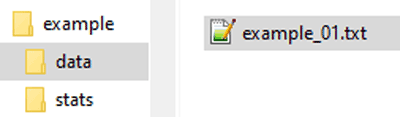
\includegraphics{pics/relative_pfad.png}

\end{tcolorbox}

\texttt{read\_delim()} verwendet eine Reihe von Heuristiken um den
jeweiligen Datentyp (numerisch, Zeichenkette, etc.) der Spalten zu
bestimmen. Der Rückgabewert von \texttt{read\_delim()} ist ein
\texttt{tibble()} der Daten. In unserem Beispiel weisen wir dem
\texttt{tibble()} den Variabllennamen \texttt{df} zu und können somit in
der weiteren Analyse mit dem Bezeichner \texttt{df} auf die Daten
zugreifen.

\begin{Shaded}
\begin{Highlighting}[]
\NormalTok{df}
\end{Highlighting}
\end{Shaded}

\begin{verbatim}
# A tibble: 4 x 3
  id    grp   value
  <chr> <chr> <dbl>
1 p1    CON       1
2 p2    CON       2
3 p3    TRT       3
4 p4    TRT       4
\end{verbatim}

Im Beispieldaten sind die ersten beiden Spalten als Zeichenketten
(\texttt{\textless{}char\textgreater{}}) erkannt worden, während die
dritte Spalte als Zahl (\texttt{\textless{}dbl\textgreater{}}) erkannt
wurde. Manchmal funktioniert die automatische Erkennung der Datentypen
nicht korrekt. In dem Falle können mit dem Parameter \texttt{col\_types}
die Spaltentypen direkt angegeben werden. Wenn keine Kopfzeile in den
Daten vorhanden ist, kann diese über den Parameter \texttt{col\_names}
spezifiziert werden. Mit \texttt{skip} können Zeilen zu Beginn der Datei
übersprungen werden.

\begin{example}[]\protect\hypertarget{exm-readr-01}{}\label{exm-readr-01}

Wollen wir zum Beispiel andere Spaltennamen haben, dann können wir die
erste Zeile beim einlesen überspringen und andere Spaltennamen angeben.

\begin{Shaded}
\begin{Highlighting}[]
\NormalTok{readr}\SpecialCharTok{::}\FunctionTok{read\_delim}\NormalTok{(}
  \AttributeTok{file =} \StringTok{\textquotesingle{}data/example\_01.txt\textquotesingle{}}\NormalTok{,}
  \AttributeTok{delim =} \StringTok{\textquotesingle{}}\SpecialCharTok{\textbackslash{}t}\StringTok{\textquotesingle{}}\NormalTok{,}
  \AttributeTok{skip =} \DecValTok{1}\NormalTok{,}
  \AttributeTok{col\_names =} \FunctionTok{c}\NormalTok{(}\StringTok{\textquotesingle{}ID\textquotesingle{}}\NormalTok{, }\StringTok{\textquotesingle{}Gruppe\textquotesingle{}}\NormalTok{,}\StringTok{\textquotesingle{}Wert\textquotesingle{}}\NormalTok{),}
  \AttributeTok{col\_types =} \StringTok{\textquotesingle{}ccd\textquotesingle{}}
\NormalTok{)}
\end{Highlighting}
\end{Shaded}

\begin{verbatim}
# A tibble: 4 x 3
  ID    Gruppe  Wert
  <chr> <chr>  <dbl>
1 p1    CON        1
2 p2    CON        2
3 p3    TRT        3
4 p4    TRT        4
\end{verbatim}

Wenn ihr das Paket \texttt{readr} vorher mit \texttt{library(readr)}
geladen habt, ist die Qualifizierung der Funktion mit \texttt{readr::}
nicht notwendig und ihr könnt direkt den Funktionsnamen verwenden. Hier
überspringen wir mit \texttt{skip=1} die erste Zeile in der Datei und
geben mit
\texttt{col\_names=c(\textquotesingle{}ID\textquotesingle{},\textquotesingle{}Gruppe\textquotesingle{},\textquotesingle{}Wert\textquotesingle{})}
eigene Spaltennamen an und spezifizieren direkt mit \texttt{col\_types}
die Dateitypen der Spalten mit \texttt{c} \(=\) \texttt{character} und
\texttt{d} = \texttt{double}.

\end{example}

Die weiteren Funktionen in \texttt{readr} wie \texttt{read\_csv},
\texttt{read\_tsv} usw. sind in den meisten Fällen Spezialversionen von
\texttt{read\_delim} bei denen der Parameter \texttt{delim} schon
voreingestellt ist. Schaut euch etwas in der
\href{https://readr.tidyverse.org/reference/index.html}{Dokumentation}
um, um einen Überblick über die verschiedenen Varianten und
Funktionalitäten zu bekommen.

\subsection{readxl}\label{readxl}

Die gleichen Daten in einer Excel-Datei können wir mit der Funktion
\texttt{read\_xlsx()} aus dem Paket \texttt{readxl} in \texttt{R} laden.
Wenn die Daten die folgende Form hat:

\begin{figure}

\centering{

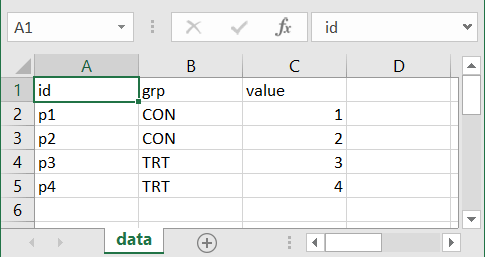
\includegraphics{pics/excel_example.png}

}

\caption{\label{fig-r-basics-excel}Beispieldatei in Excel}

\end{figure}%

dann können wir die Daten mit dem folgenden Befehl laden:

\begin{Shaded}
\begin{Highlighting}[]
\NormalTok{df }\OtherTok{\textless{}{-}}\NormalTok{ readxl}\SpecialCharTok{::}\FunctionTok{read\_xlsx}\NormalTok{(}
  \AttributeTok{path =} \StringTok{\textquotesingle{}data/example\_01.xlsx\textquotesingle{}}\NormalTok{,}
  \AttributeTok{sheet =} \StringTok{\textquotesingle{}data\textquotesingle{}}\NormalTok{,}
  \AttributeTok{range =} \StringTok{\textquotesingle{}A1:C5\textquotesingle{}}
\NormalTok{)}
\NormalTok{df}
\end{Highlighting}
\end{Shaded}

\begin{verbatim}
# A tibble: 4 x 3
  id    grp   value
  <chr> <chr> <dbl>
1 p1    CON       1
2 p2    CON       2
3 p3    TRT       3
4 p4    TRT       4
\end{verbatim}

Ähnlich wie bei \texttt{read\_delim()} geben wir mit \texttt{path} den
Pfad zur Datei an. Der Parameter \texttt{sheet} spezifiziert aus welchem
Excelblatt die Daten einlesen werden sollen, während der Parameter
\texttt{range} den Datenbereich auf dem Blatt definieren. Je nachdem wie
kompliziert eure Exceldatei aussieht müssen \texttt{sheet} und
\texttt{range} oft gar nicht angegeben werden da \texttt{read\_xlsx()}
auch über heuristische Regeln versucht zu erraten welche Daten ihr
einlesen wollt. Allerdings ist dies eher eine fragile Annahme und daher
im Sinne einer robusten Datenanalyse ist zu empfehlen beide Parameter
immer anzugeben und sicherzugehen das auch wirklich die gewollten Daten
eingelesen werden.

\begin{tcolorbox}[enhanced jigsaw, bottomrule=.15mm, breakable, leftrule=.75mm, left=2mm, toptitle=1mm, opacitybacktitle=0.6, bottomtitle=1mm, colframe=quarto-callout-note-color-frame, titlerule=0mm, colback=white, colbacktitle=quarto-callout-note-color!10!white, toprule=.15mm, opacityback=0, arc=.35mm, rightrule=.15mm, title=\textcolor{quarto-callout-note-color}{\faInfo}\hspace{0.5em}{Note}, coltitle=black]

Bei Parameter \texttt{range} darauf achten, das dieser bei Veränderung
der Excel-Datei, z.B. wenn neue Daten dazukommen entsprechend angepasst
wird.

\end{tcolorbox}

\subsection{haven}\label{haven}

Im Paket \texttt{haven} haben wir Funktionen um mit SPSS-Dateien (siehe
Figure~\ref{fig-r-basics-spss}) zu arbeiten.

\begin{figure}

\centering{

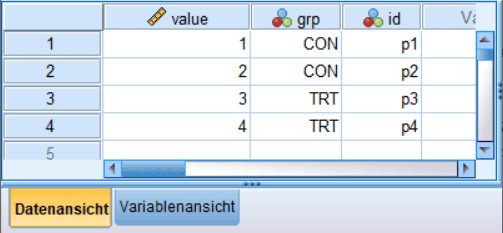
\includegraphics{pics/spss_example.png}

}

\caption{\label{fig-r-basics-spss}Beispieldatei in SPSS}

\end{figure}%

Die Funktionen funktionen zum Glück selbst wenn SPSS auf dem Rechner
nicht installiert ist. Allerdings kann hier nicht nachkontrolliert
werden ob das Einlesen korrekt stattgefunden hat, wenn keine
Dokumentation zu den Daten vorhanden ist. In SPSS werden Datein
üblicherweise in einem binären \texttt{sav}-Dateikontainer gespeichert.
In \texttt{R} können die Daten mittels der Funktion \texttt{read\_sav()}
aus dem Paket \texttt{haven} eingelesen werden.

\begin{Shaded}
\begin{Highlighting}[]
\NormalTok{df }\OtherTok{\textless{}{-}}\NormalTok{ haven}\SpecialCharTok{::}\FunctionTok{read\_sav}\NormalTok{(}\StringTok{\textquotesingle{}data/example\_01.sav\textquotesingle{}}\NormalTok{)}
\NormalTok{df}
\end{Highlighting}
\end{Shaded}

\begin{verbatim}
# A tibble: 4 x 3
  value grp       id       
  <dbl> <dbl+lbl> <dbl+lbl>
1     1 1 [CON]   1 [p1]   
2     2 1 [CON]   2 [p2]   
3     3 2 [TRT]   3 [p3]   
4     4 2 [TRT]   4 [p4]   
\end{verbatim}

Da SPSS eigene Datentypen, insbesondere im Zusammenhang mit nominalen
bzw. ordinalen Variablen hat, sind im Paket \texttt{haven} spezielle
Datentypen definiert. Im Beispiel hier ersichtlich am Datentyp für
\texttt{grp} mit \texttt{\textless{}dbl+lbl\textgreater{}}. Es handelt
sich hier um den Datentypen \texttt{labelled}. In der Dokumentation von
\texttt{read\_sav()} gibt es hierzu weiter Informationen.

\begin{tcolorbox}[enhanced jigsaw, bottomrule=.15mm, breakable, leftrule=.75mm, left=2mm, toptitle=1mm, opacitybacktitle=0.6, bottomtitle=1mm, colframe=quarto-callout-tip-color-frame, titlerule=0mm, colback=white, colbacktitle=quarto-callout-tip-color!10!white, toprule=.15mm, opacityback=0, arc=.35mm, rightrule=.15mm, title=\textcolor{quarto-callout-tip-color}{\faLightbulb}\hspace{0.5em}{Tip}, coltitle=black]

Mit der Funktion \texttt{as\_factor()} aus dem Paket \texttt{haven}
können die \texttt{labelled} Daten in den \texttt{R} Dateityp
\texttt{factor} umgewandelt werden.

\end{tcolorbox}

Wenn wir die Daten in \texttt{R} eingelesen haben, können wir nun als
nächstes die Daten verarbeiten und so strukturieren wie wir sie für die
weitere Analyse benötigen. Dazu stehen uns eine Reihe von weiteren
Funktionen aus dem \texttt{tidyverse} zur verfügung.

\section{\texorpdfstring{Daten in \texttt{R} prozessieren mit
\texttt{tidyverse}}{Daten in R prozessieren mit tidyverse}}\label{daten-in-r-prozessieren-mit-tidyverse}

Die Art der Programmierung im \texttt{tidyverse} verwendet oft eine
eigene Herangehensweise die sich vonderjenigen die wir bisher
kennengelernt haben etwas unterscheidet. Um den Code leserlich zu halten
werden mehrere Funktionen in sogenannten \emph{pipes} aneinandergehängt
ohne zwischendrin temporäre Variablen zu erstellen. Dies führt zu Code
der fast wie Prosa gelesen werden kann. Dazu müssenw wir aber zunächst
einen neuen Operator kennenlernen.

\subsection{\texorpdfstring{Der Pipe operator
\texttt{\textbar{}\textgreater{}}}{Der Pipe operator \textbar\textgreater{}}}\label{der-pipe-operator}

In \texttt{R} gibt es den sogenannten pipe-operator
\texttt{\textbar{}\textgreater{}}. Der \texttt{\textbar{}\textgreater{}}
hat die Eigenschaft, dass ein vorangestellter Wert (dies kann auch der
Rückgabewert einer Funktion sein) als das erste Argument an eine
nachfolgende Funktion übergeben wird. Dies ermöglicht es Code zu
schreiben der sich wie gesprochener Text liest. Schauen wir uns ein
einfaches Beispiel an. Wir wollen den Mittelwert eines Zahlenvektors
berechnen und anschließend das Ergebnis auf die zweite Nachkommastelle
runden. Normalerweise würden wir das wie folgt formulieren wenn wir
keine Zwischenvariablen definieren wollen.

\begin{Shaded}
\begin{Highlighting}[]
\NormalTok{vec }\OtherTok{\textless{}{-}} \FunctionTok{c}\NormalTok{(}\DecValTok{1}\NormalTok{, }\DecValTok{7}\NormalTok{, }\DecValTok{3}\NormalTok{, }\SpecialCharTok{{-}}\FloatTok{5.22}\NormalTok{, }\DecValTok{5}\NormalTok{, }\FloatTok{6.3}\NormalTok{)}
\FunctionTok{round}\NormalTok{(}\FunctionTok{mean}\NormalTok{(vec), }\DecValTok{2}\NormalTok{)}
\end{Highlighting}
\end{Shaded}

\begin{verbatim}
[1] 2.85
\end{verbatim}

D.h. wir haben ein Schachtelung (nesting) der Funktionen. Die
\texttt{mean()} Funktion ist innerhalb der \texttt{round()} Funktion
geschachtelt bzw. der Rückgabewert von \texttt{mean()} wird als erstes
Argument an \texttt{round()} übergeben. Schauen wir uns nun an, wie wir
das gleiche Programm mit dem pipe-operator
\texttt{\textbar{}\textgreater{}} formulieren.

\begin{Shaded}
\begin{Highlighting}[]
\NormalTok{vec }\SpecialCharTok{|\textgreater{}} \FunctionTok{mean}\NormalTok{() }\SpecialCharTok{|\textgreater{}} \FunctionTok{round}\NormalTok{(}\DecValTok{2}\NormalTok{)}
\end{Highlighting}
\end{Shaded}

\begin{verbatim}
[1] 2.85
\end{verbatim}

Was ist hier passiert? Die erste pipe \texttt{\textbar{}\textgreater{}}
übergibt ihr links stehendes Argument, den Vektor \texttt{vec} and das
erste Argument der rechts stehenden Funktion \texttt{mean()}. Aus
\texttt{vec\ \textbar{}\textgreater{}\ mean()} wird \texttt{mean(vec)}.
\texttt{mean()} ist happy und berechnet den Mittelwert des Vektors der
nun als Rückgabewert zur Verfügung steht. Der zweite pipe-Operator und
nimmt nun wieder diesen \emph{linke} Wert, der berechnete Mittelwert,
und übergibt diesen an das erste Argument der nachfolgenden
\texttt{round(2)}-Funktion. Wenn ihr euch die Hilfe von \texttt{round()}
anschaut, dann seht ihr, dass dere erste Parmeter der zu rundende Wert
ist. Was macht jetzt aber die \texttt{2} in \texttt{round(2)}. Nun,
\texttt{\textbar{}\textgreater{}} stellt den links stehenden Wert an die
erste Stelle der rechts stehenden Funktion, dadurch rutscht die
\texttt{2} an die zweite Argumentenstelle in \texttt{round()} und
bestimmt somit die Anzahl der zu runden Stellen.

Der Vorteil des pipe-Operators ist, dass ihr das Program nun einfach von
links nach rechts lesen könnt. Nimm \texttt{vec}, stecke es in
\texttt{mean()} und stecke das was rauskommt in \texttt{round(2)}. Bei
dem ursprünglichen Programm musstet ihr euch von innen nach außen
arbeiten und dabei immer im Blick behalten auf welcher Stufe ihr seid um
die Parameterzuordnung richtig interpretieren zu können.

Noch ein Beispiel, wir wollen den Mittelwert auf den Absolutwerten des
Vektors berechnen. Nach der Standardmethode.

\begin{Shaded}
\begin{Highlighting}[]
\FunctionTok{round}\NormalTok{(}\FunctionTok{mean}\NormalTok{(}\FunctionTok{abs}\NormalTok{(vec)), }\DecValTok{2}\NormalTok{)}
\end{Highlighting}
\end{Shaded}

\begin{verbatim}
[1] 4.59
\end{verbatim}

Mit dem pipe-Operator

\begin{Shaded}
\begin{Highlighting}[]
\NormalTok{vec }\SpecialCharTok{|\textgreater{}} \FunctionTok{abs}\NormalTok{() }\SpecialCharTok{|\textgreater{}} \FunctionTok{mean}\NormalTok{() }\SpecialCharTok{|\textgreater{}} \FunctionTok{round}\NormalTok{(}\DecValTok{2}\NormalTok{)}
\end{Highlighting}
\end{Shaded}

\begin{verbatim}
[1] 4.59
\end{verbatim}

Wenn die pipe Anfängt zu lang zu werden, dann hat es sich einbürgert
nach der pipe eine neue Zeile anzufangen.

\begin{Shaded}
\begin{Highlighting}[]
\NormalTok{vec }\SpecialCharTok{|\textgreater{}} \FunctionTok{abs}\NormalTok{() }\SpecialCharTok{|\textgreater{}} 
  \FunctionTok{mean}\NormalTok{() }\SpecialCharTok{|\textgreater{}} \FunctionTok{round}\NormalTok{(}\DecValTok{2}\NormalTok{)}
\end{Highlighting}
\end{Shaded}

\begin{verbatim}
[1] 4.59
\end{verbatim}

Der pipe-Operator \texttt{\textbar{}\textgreater{}} ist so alltäglich,
dass ihr in RStudio einen short-cut für ihn habt \texttt{STRG+SHIFT+m}.

Bei der Vewendung der pipe dabei nicht vergessen das Ergebnis der pipe
dann letztendlich doch wieder eine Variable zuzuweisen. Ansonsten
berechnet \texttt{R} den Wert und schmeißt ihn gleich wieder weg.

\begin{verbatim}
[1] 4.59
\end{verbatim}

Der pipe-Operator \texttt{\textbar{}\textgreater{}} ist im alltäglichen
Umgang mit Datenprozessierung im Zusammenhang mit \texttt{tidyverse}
praktisch unabkömmlich und praktisch jegliche Codeschnipsel die ihr im
Netz dazu findet verwenden pipes. Tatsächlich ist die dahinterliegende
Idee in der Informatik (siehe Kernighan and Pike 1984) schon relativ
lange bekannt. Die darüberliegende Idee ist nämlich Anstatt große,
komplizierte Funktionen zu schreiben die eine Vielzahl von Argumenten
haben und mehrere unterschiedliche Aufgaben erledigen, werden lieber
viele kleine, spezialisierte Programme zu erstellen. Die spezialisierten
Programme können dann zusamengesetzt werden um komplizierte Aufgaben zu
erfüllen. Der pipe-operator ist dabei zentral für diese Idee, da er es
ermöglicht die spezialisierten, kleinen Programmen einfach aneinander zu
hängen. Ähnlich wie zum Beispiel bei einen Kinderwasserspielzeug mit
Rohren, Schaufeln und Filtern können durchumordnung der Einzelfunktion
beliebig komplexe Mechanismen abgebildet werden. Unter Linux bash ist
daher auch ein pipe-Operator \texttt{\textbar{}} zu finden.

Nach diesem Ausflug zurück zur Datenbearbeitung mit dem
\texttt{tidyverse}. Um die Daten möglichst einfach mit dem
\texttt{tidyverse} verarbeiten zu können, sollten die Daten im
\texttt{tibble()} einer bestimmten Struktur folgen. Im
\texttt{tidyverse} wird diese Anordnung als \emph{tidy-Data} bezeichnet.

\subsection{tidy-Data}\label{tidy-data}

Zu tidy-Data gibt es in der einfachsten Form nur drei Regeln die zu
beachten sind:

\begin{enumerate}
\def\labelenumi{\arabic{enumi}.}
\tightlist
\item
  Jede Spalte ist eine Variable
\item
  Jede Zeile ist eine Beobachtung
\item
  Jede Zelle ist ein einzelner Eintrag
\end{enumerate}

Schauen wir uns wieder ein einfaches, fiktives Beispiel mit Sprunghöhen
an.

\begin{Shaded}
\begin{Highlighting}[]
\NormalTok{df }\OtherTok{\textless{}{-}} \FunctionTok{tibble}\NormalTok{(}
  \AttributeTok{time =} \FunctionTok{rep}\NormalTok{(}\FunctionTok{c}\NormalTok{(}\StringTok{\textquotesingle{}pre\textquotesingle{}}\NormalTok{,}\StringTok{\textquotesingle{}post\textquotesingle{}}\NormalTok{), }\DecValTok{4}\NormalTok{),}
  \AttributeTok{gender =} \FunctionTok{rep}\NormalTok{(}\FunctionTok{c}\NormalTok{(}\StringTok{\textquotesingle{}m\textquotesingle{}}\NormalTok{,}\StringTok{\textquotesingle{}f\textquotesingle{}}\NormalTok{), }\AttributeTok{each=}\DecValTok{4}\NormalTok{),}
  \AttributeTok{age =} \FunctionTok{rep}\NormalTok{(}\FunctionTok{round}\NormalTok{(}\FunctionTok{runif}\NormalTok{(}\DecValTok{4}\NormalTok{, }\DecValTok{20}\NormalTok{, }\DecValTok{40}\NormalTok{)),}\AttributeTok{each=}\DecValTok{2}\NormalTok{),}
  \AttributeTok{cmj =} \FunctionTok{round}\NormalTok{(}\FunctionTok{rnorm}\NormalTok{(}\DecValTok{8}\NormalTok{, }\FunctionTok{c}\NormalTok{(}\DecValTok{25}\NormalTok{,}\DecValTok{20}\NormalTok{), }\DecValTok{2}\NormalTok{), }\DecValTok{1}\NormalTok{)}
\NormalTok{)}
\NormalTok{df}
\end{Highlighting}
\end{Shaded}

\begin{verbatim}
# A tibble: 8 x 4
  time  gender   age   cmj
  <chr> <chr>  <dbl> <dbl>
1 pre   m         26  25.9
2 post  m         26  18.8
3 pre   m         21  24.5
4 post  m         21  22.1
5 pre   f         23  26.7
6 post  f         23  20.7
7 pre   f         22  23.4
8 post  f         22  19.4
\end{verbatim}

Wir haben vier Spalten, \texttt{time}, \texttt{gender}, \texttt{age} und
\texttt{cmj} die jeweils eine Variable darstellen. In jeder Zeile ist
eine Beobachtung eine Sprunghöhe \texttt{cmj} einer Person eines Alters
\texttt{age} und \texttt{gender} zu einem bestimmten Zeitpunkt
\texttt{time}. Schaut also tidy aus.

Diese Darstellung ist aber wahrscheinlich unterschiedlich zu derjenigen
wie ihr solche Daten schon öfter gesehen habt. Wahrscheinlich nämlich
eher so.

\begin{verbatim}
# A tibble: 4 x 4
  gender   age   pre  post
  <chr>  <dbl> <dbl> <dbl>
1 m         26  25.9  18.8
2 m         21  24.5  22.1
3 f         23  26.7  20.7
4 f         22  23.4  19.4
\end{verbatim}

Diese Darstellung ist zwar kompakter aber entspricht nicht mehr den
tidy-Anforderungen, da wir nun nicht mehr nur eine Beobachtung pro Zeile
haben. Wir haben für jede Person die Sprunghöhe zu zwei Zeitpunkten in
einer Zeile. Die Daten sind in dieser Darstellung also \emph{untidy}.
Die \emph{tidy}-Version ist etwas länger und enthält redundante
Informationen aber wir werden im Folgenden sehen, dass diese Darstellung
in der Verarbeitung zahlreiche Vorteile hat. Dazu werden wir auch
Funktionen kennenlernen mit denen wir zwischen diesen beiden Formaten
hin- und herwechseln können. Die \emph{tidy}-Darstellung wird als
long-Format bezeichnet, während die \emph{untidy}-Darstellung als
wide-Format bezeichnet wird.

\subsection{\texorpdfstring{\texttt{filter()}}{filter()}}\label{filter}

Lernen wir jezt unseren ersten \texttt{tidyverse()} Befehl zur
Datenmanipulation kennen. Die Befehle werden als Verben bezeichnet und
die Regel für die Funktionennahmen ist zum Glück ziemlich einfach:``was
im Namen draufsteht ist auch in der Packung drin''. Der Befehl
\texttt{filter} filtert Daten, d.h. wir geben einen Sack Daten rein und
wollen nur einen Teil wieder raus haben der bestimmte Eigenschaften hat.
Dazu können wir einfache Regel mittels der Vergleichsoperatoren in
\texttt{filter()} zusammen mit den Spaltennahmen im \texttt{tibble()}
verwenden. Wollen wir aus unserem Datensatz nur alle weiblichen
Datenpunkte herausfiltern und wir wissen, dass die Information über das
Gender in der Spalte \texttt{gender} steht und mit \texttt{f} für
weiblich kodiert ist, dann können wir mit dem Vergleich `gender == `f'
die Daten entsprechen filtern.

\begin{Shaded}
\begin{Highlighting}[]
\NormalTok{df }\SpecialCharTok{|\textgreater{}} \FunctionTok{filter}\NormalTok{(gender }\SpecialCharTok{==} \StringTok{\textquotesingle{}f\textquotesingle{}}\NormalTok{)}
\end{Highlighting}
\end{Shaded}

\begin{verbatim}
# A tibble: 4 x 4
  time  gender   age   cmj
  <chr> <chr>  <dbl> <dbl>
1 pre   f         23  26.7
2 post  f         23  20.7
3 pre   f         22  23.4
4 post  f         22  19.4
\end{verbatim}

Wollen wir dagegen auf das Alter mit \texttt{age\ \textless{}\ 30}
filtern, verwenden wir:

\begin{Shaded}
\begin{Highlighting}[]
\NormalTok{df }\SpecialCharTok{|\textgreater{}} \FunctionTok{filter}\NormalTok{(age }\SpecialCharTok{\textless{}} \DecValTok{30}\NormalTok{)}
\end{Highlighting}
\end{Shaded}

\begin{verbatim}
# A tibble: 8 x 4
  time  gender   age   cmj
  <chr> <chr>  <dbl> <dbl>
1 pre   m         26  25.9
2 post  m         26  18.8
3 pre   m         21  24.5
4 post  m         21  22.1
5 pre   f         23  26.7
6 post  f         23  20.7
7 pre   f         22  23.4
8 post  f         22  19.4
\end{verbatim}

Wenn die Daten mehrere Konditionen erfüllen müssen, verwenden wir
entsprechend mehrere Filteranweisungen. Die Vergleiche werden intern
mittels einer Und-Operation zusammengesetzt.

\begin{Shaded}
\begin{Highlighting}[]
\NormalTok{df }\SpecialCharTok{|\textgreater{}} \FunctionTok{filter}\NormalTok{(age }\SpecialCharTok{\textless{}} \DecValTok{25}\NormalTok{, gender }\SpecialCharTok{==} \StringTok{\textquotesingle{}f\textquotesingle{}}\NormalTok{)}
\end{Highlighting}
\end{Shaded}

\begin{verbatim}
# A tibble: 4 x 4
  time  gender   age   cmj
  <chr> <chr>  <dbl> <dbl>
1 pre   f         23  26.7
2 post  f         23  20.7
3 pre   f         22  23.4
4 post  f         22  19.4
\end{verbatim}

\texttt{filter()} gibt uns in diesem Bespiel also alle Datenpunkte
zurück bei denen \texttt{age\ \textless{}\ 25} und
\texttt{gender\ ==\ \textquotesingle{}f\textquotesingle{}} gilt. Durch
die Kombination von mehreren Vergleichen können relativ einfach komplexe
Bedingungen formuliert werden.

\begin{tcolorbox}[enhanced jigsaw, bottomrule=.15mm, breakable, leftrule=.75mm, left=2mm, toptitle=1mm, opacitybacktitle=0.6, bottomtitle=1mm, colframe=quarto-callout-tip-color-frame, titlerule=0mm, colback=white, colbacktitle=quarto-callout-tip-color!10!white, toprule=.15mm, opacityback=0, arc=.35mm, rightrule=.15mm, title=\textcolor{quarto-callout-tip-color}{\faLightbulb}\hspace{0.5em}{Tip}, coltitle=black]

Manchmal möchte wir nur alle vollständigen Zeilen aus einen Datensatz
weiterverwenden. Dies könnten wir mit \texttt{filter()} erreichen, dazu
müssten wir aber für jede Spalte einen Vergleich mit \texttt{is.na()}
schreiben wenn die fehlenden Werte \texttt{NA} über mehrere Spalten
verteilt sind. Schneller geht dies mit dem Befehlt \texttt{drop\_na()}.

\begin{Shaded}
\begin{Highlighting}[]
\NormalTok{df\_missing }\OtherTok{\textless{}{-}} \FunctionTok{tibble}\NormalTok{(}\AttributeTok{x =} \DecValTok{1}\SpecialCharTok{:}\DecValTok{4}\NormalTok{, }\AttributeTok{y =} \FunctionTok{c}\NormalTok{(}\DecValTok{11}\NormalTok{,}\ConstantTok{NA}\NormalTok{,}\DecValTok{13}\NormalTok{,}\DecValTok{14}\NormalTok{), }\AttributeTok{z =} \FunctionTok{c}\NormalTok{(}\DecValTok{21}\NormalTok{,}\DecValTok{22}\NormalTok{,}\DecValTok{23}\NormalTok{,}\ConstantTok{NA}\NormalTok{))}
\NormalTok{df\_missing}
\end{Highlighting}
\end{Shaded}

\begin{verbatim}
# A tibble: 4 x 3
      x     y     z
  <int> <dbl> <dbl>
1     1    11    21
2     2    NA    22
3     3    13    23
4     4    14    NA
\end{verbatim}

\begin{Shaded}
\begin{Highlighting}[]
\NormalTok{df\_missing }\SpecialCharTok{|\textgreater{}} \FunctionTok{drop\_na}\NormalTok{()}
\end{Highlighting}
\end{Shaded}

\begin{verbatim}
# A tibble: 2 x 3
      x     y     z
  <int> <dbl> <dbl>
1     1    11    21
2     3    13    23
\end{verbatim}

\end{tcolorbox}

Insgesamt führt \texttt{filter()} in den meisten Fällen dazu, dass wir
ein \texttt{tibble} mit weniger Zeilen als ursprünglich erhalten.

\subsection{\texorpdfstring{\texttt{select()}}{select()}}\label{select}

Das nächste Verb aus dem \texttt{tidyverse} ist \texttt{select()}. Mit
\texttt{select()} können wir einzelne Variablen/Spalten aus einem
\texttt{tibble()} selektieren. Wollen wir zum Beispiel aus unserem
Datensatz nur die beiden Spalten \texttt{time} und \texttt{gender}
auswählen, dann können wir dies mit \texttt{select()} wie folgt
formulieren:

\begin{Shaded}
\begin{Highlighting}[]
\NormalTok{df }\SpecialCharTok{|\textgreater{}} \FunctionTok{select}\NormalTok{(time, gender)}
\end{Highlighting}
\end{Shaded}

\begin{verbatim}
# A tibble: 8 x 2
  time  gender
  <chr> <chr> 
1 pre   m     
2 post  m     
3 pre   m     
4 post  m     
5 pre   f     
6 post  f     
7 pre   f     
8 post  f     
\end{verbatim}

Der Rückgabewert von \texttt{select()} ist entsprechend ein
\texttt{tibble} das nur die selektierten Spalten enthält. Ähnlich wie
das auch bei der Indexierung von Elementen in Vektoren funktioniert
versteht \texttt{select()} auch eine Ausschlusssyntax mit \texttt{-}.
Wollen wir z.B. alle Spalten aus \texttt{gender} formulieren wir dies
wie folgt:

\begin{Shaded}
\begin{Highlighting}[]
\NormalTok{df }\SpecialCharTok{|\textgreater{}} \FunctionTok{select}\NormalTok{(}\SpecialCharTok{{-}}\NormalTok{gender)}
\end{Highlighting}
\end{Shaded}

\begin{verbatim}
# A tibble: 8 x 3
  time    age   cmj
  <chr> <dbl> <dbl>
1 pre      26  25.9
2 post     26  18.8
3 pre      21  24.5
4 post     21  22.1
5 pre      23  26.7
6 post     23  20.7
7 pre      22  23.4
8 post     22  19.4
\end{verbatim}

\begin{example}[]\protect\hypertarget{exm-select-01}{}\label{exm-select-01}

Da wir jetzt schon zwei Verben kennen, können wir auch direkt sehen wie
wir durch die Kombination der Befehle komplexere Anweisungen relativ
einfach in Code übersetzen können. Wollen wir zum Beispiel alle
Datenpunkte von Frauen die älter als 28 sind verwenden und brauch dann
nicht mehr die \texttt{gender} Variable könen wir dies wie folgt
übersetzen:

\begin{Shaded}
\begin{Highlighting}[]
\NormalTok{df }\SpecialCharTok{|\textgreater{}} \FunctionTok{filter}\NormalTok{(gender }\SpecialCharTok{==} \StringTok{\textquotesingle{}f\textquotesingle{}}\NormalTok{, age }\SpecialCharTok{\textgreater{}} \DecValTok{27}\NormalTok{) }\SpecialCharTok{|\textgreater{}} \FunctionTok{select}\NormalTok{(}\SpecialCharTok{{-}}\NormalTok{gender)}
\end{Highlighting}
\end{Shaded}

\begin{verbatim}
# A tibble: 0 x 3
# i 3 variables: time <chr>, age <dbl>, cmj <dbl>
\end{verbatim}

\end{example}

Insgesamt führt \texttt{select()} dazu, dass wir ein \texttt{tibble}
erhalten, dass weniger Spalten als ursprünglich enthält.

\subsection{\texorpdfstring{\texttt{mutate()}}{mutate()}}\label{mutate}

In den beiden vorhergehenden Fällen, haben wir die Daten nicht wirklich
verändert sondern entweder nur bestimmte Fälle mit \texttt{filter()}
oder bestimmte Variablen mit \texttt{select()} ausgewählt. Oft kommt es
aber vor, dass wir aus den bestehenden Daten neue Daten erstellen
wollen. Um neue Daten zu berechnen verwenden wir im \texttt{tidyverse}
das Verb \texttt{mutate()}.

In unserem Datensatz liegen die Sprunhöhen in Zentimeter vor, wir
benötigen aber für weitere Berechnungen die Sprunghöhen in Metern. Dazu
wollen wir eine neue Spalte erstellen, die wir, um sie von der anderen
Spalte abzugrenzen, mit \texttt{cmj\_m} bezeichnen wollen. Dazu setzen
wir \texttt{mutate()} wie folgt ein.

\begin{Shaded}
\begin{Highlighting}[]
\NormalTok{df }\SpecialCharTok{|\textgreater{}} \FunctionTok{mutate}\NormalTok{(}\AttributeTok{cmj\_m =}\NormalTok{ cmj }\SpecialCharTok{/} \DecValTok{100}\NormalTok{)}
\end{Highlighting}
\end{Shaded}

\begin{verbatim}
# A tibble: 8 x 5
  time  gender   age   cmj cmj_m
  <chr> <chr>  <dbl> <dbl> <dbl>
1 pre   m         26  25.9 0.259
2 post  m         26  18.8 0.188
3 pre   m         21  24.5 0.245
4 post  m         21  22.1 0.221
5 pre   f         23  26.7 0.267
6 post  f         23  20.7 0.207
7 pre   f         22  23.4 0.234
8 post  f         22  19.4 0.194
\end{verbatim}

Wie sehen, dass eine neue Spalte in dem \texttt{tibble} erstellt wurde
mit eben der Namen \texttt{cmj\_m}.

\begin{tcolorbox}[enhanced jigsaw, bottomrule=.15mm, breakable, leftrule=.75mm, left=2mm, toptitle=1mm, opacitybacktitle=0.6, bottomtitle=1mm, colframe=quarto-callout-warning-color-frame, titlerule=0mm, colback=white, colbacktitle=quarto-callout-warning-color!10!white, toprule=.15mm, opacityback=0, arc=.35mm, rightrule=.15mm, title=\textcolor{quarto-callout-warning-color}{\faExclamationTriangle}\hspace{0.5em}{Warning}, coltitle=black]

\texttt{mutate()} verhindert nicht, Variablen mit neuen Werten zu
überschreiben. Würden wir die Sprunghöhen in Zentimeter später nicht
mehr benötigen, könnten wir die Spalte \texttt{cmj} auch überschreiben.

\begin{Shaded}
\begin{Highlighting}[]
\NormalTok{df }\SpecialCharTok{|\textgreater{}} \FunctionTok{mutate}\NormalTok{(}\AttributeTok{cmj =}\NormalTok{ cmj }\SpecialCharTok{/} \DecValTok{100}\NormalTok{)}
\end{Highlighting}
\end{Shaded}

\begin{verbatim}
# A tibble: 8 x 4
  time  gender   age   cmj
  <chr> <chr>  <dbl> <dbl>
1 pre   m         26 0.259
2 post  m         26 0.188
3 pre   m         21 0.245
4 post  m         21 0.221
5 pre   f         23 0.267
6 post  f         23 0.207
7 pre   f         22 0.234
8 post  f         22 0.194
\end{verbatim}

\end{tcolorbox}

Der große Vorteil von \texttt{mutate()} ist hier auch wieder, das wir
direkt auf die Spaltenahmen zugreifen können und nicht wie sonst
notwendig den \texttt{\$}-Operator.

Durch \texttt{mutate()} werden insgesamt also zusätzliche Spalten an das
ursprüngliche \texttt{tibble} angehängt.

\begin{example}[]\protect\hypertarget{exm-mutate-01}{}\label{exm-mutate-01}

Aufbauend auf dem Beispiel von eben, wollen wir zum Beispiel die Spalte
mit Sprunghöhen nicht beibehalten aber einen neuen Namen verwenden damit
wir später nachvollziehen können, dass wir die Sprunghöhen bearbeitet
haben, könnten wir wieder mit einer Kombination der Verben
\texttt{mutate()} und \texttt{select()} in einer pipe vorgehen:

\begin{Shaded}
\begin{Highlighting}[]
\NormalTok{df }\SpecialCharTok{|\textgreater{}} \FunctionTok{mutate}\NormalTok{(}\AttributeTok{cmj\_m =}\NormalTok{ cmj }\SpecialCharTok{/} \DecValTok{100}\NormalTok{) }\SpecialCharTok{|\textgreater{}} \FunctionTok{select}\NormalTok{(}\SpecialCharTok{{-}}\NormalTok{cmj)}
\end{Highlighting}
\end{Shaded}

\begin{verbatim}
# A tibble: 8 x 4
  time  gender   age cmj_m
  <chr> <chr>  <dbl> <dbl>
1 pre   m         26 0.259
2 post  m         26 0.188
3 pre   m         21 0.245
4 post  m         21 0.221
5 pre   f         23 0.267
6 post  f         23 0.207
7 pre   f         22 0.234
8 post  f         22 0.194
\end{verbatim}

\end{example}

\subsection{\texorpdfstring{\texttt{summarize()}}{summarize()}}\label{summarize}

Mit der \texttt{summarize()} Funktion werden alle Beobachtung (Zeilen)
in eine Zeile zusammengefasst. Wollen wir zum Beispiel die
durchschnittliche Sprunghöhe über alle Beobachtung berechnen.

\begin{Shaded}
\begin{Highlighting}[]
\NormalTok{df }\SpecialCharTok{|\textgreater{}} \FunctionTok{summarize}\NormalTok{(}\AttributeTok{cmj\_bar =} \FunctionTok{mean}\NormalTok{(cmj))}
\end{Highlighting}
\end{Shaded}

\begin{verbatim}
# A tibble: 1 x 1
  cmj_bar
    <dbl>
1    22.7
\end{verbatim}

\texttt{summarize()} kann auch mehrere Werte berechnen.

\begin{Shaded}
\begin{Highlighting}[]
\NormalTok{df }\SpecialCharTok{|\textgreater{}} \FunctionTok{summarize}\NormalTok{(}\AttributeTok{cmj\_bar =} \FunctionTok{mean}\NormalTok{(cmj), }\AttributeTok{age\_bar =} \FunctionTok{mean}\NormalTok{(age))}
\end{Highlighting}
\end{Shaded}

\begin{verbatim}
# A tibble: 1 x 2
  cmj_bar age_bar
    <dbl>   <dbl>
1    22.7      23
\end{verbatim}

\subsection{\texorpdfstring{\texttt{group\_by()}}{group\_by()}}\label{group_by}

Die \texttt{summarize()} Funktion wird tatsächlich erst richtig mächtig
im Zusammenhang mit der \texttt{group\_by()} Funktion. Mit
\texttt{group\_by()} kann ein Datensatz anhand der Werte einer Variable
in Untergruppen geschnitten werden. Wollen wir in unserem Beispiel die
Mittelwerte für verschiedenen Zeitpunkte berechnen.

\begin{Shaded}
\begin{Highlighting}[]
\NormalTok{df }\SpecialCharTok{|\textgreater{}} \FunctionTok{group\_by}\NormalTok{(time) }\SpecialCharTok{|\textgreater{}} \FunctionTok{summarize}\NormalTok{(}\AttributeTok{cmj\_bar =} \FunctionTok{mean}\NormalTok{(cmj))}
\end{Highlighting}
\end{Shaded}

\begin{verbatim}
# A tibble: 2 x 2
  time  cmj_bar
  <chr>   <dbl>
1 post     20.2
2 pre      25.1
\end{verbatim}

Das gruppieren funktioniert auch über mehrere Variablen.

\begin{Shaded}
\begin{Highlighting}[]
\NormalTok{df }\SpecialCharTok{|\textgreater{}} \FunctionTok{group\_by}\NormalTok{(time, gender) }\SpecialCharTok{|\textgreater{}} \FunctionTok{summarize}\NormalTok{(}\AttributeTok{cmj\_bar =} \FunctionTok{mean}\NormalTok{(cmj))}
\end{Highlighting}
\end{Shaded}

\begin{verbatim}
# A tibble: 4 x 3
# Groups:   time [2]
  time  gender cmj_bar
  <chr> <chr>    <dbl>
1 post  f         20.0
2 post  m         20.5
3 pre   f         25.0
4 pre   m         25.2
\end{verbatim}

Die Kombination aus \texttt{filter()}, \texttt{group\_by()} und
\texttt{summarize()} deckt wahrscheinlich mehr als die Hälfte der
Anwendungen bei der Datenanalyse ab. Die folgenden Befehle sind etwas
spezialisiert.

\subsection{\texorpdfstring{\texttt{separate()}}{separate()}}\label{separate}

Mit dem \texttt{separate()} Befehle kann eine Variable in der mehrere
Informationen gespeichert sind, in mehrere Variablen separiert werden.

\begin{verbatim}
# A tibble: 4 x 2
  Kondition  wert
  <chr>     <int>
1 pre_trt       1
2 post_trt      2
3 pre_con       3
4 post_con      4
\end{verbatim}

Die Variable Kondition hat zwei Variablen in einer kodiert
(\emph{untidy}). Mit \texttt{separate()} können wir Kondition aufteilen.
\texttt{separate()} benötigt als Parameter neben dem Spaltennamen eine
Vector der neuen Spaltennamen übergeben an das Funktionsargument
\texttt{into}.

\begin{Shaded}
\begin{Highlighting}[]
\NormalTok{df\_2 }\SpecialCharTok{|\textgreater{}} \FunctionTok{separate}\NormalTok{(Kondition, }\AttributeTok{into=}\FunctionTok{c}\NormalTok{(}\StringTok{\textquotesingle{}time\textquotesingle{}}\NormalTok{,}\StringTok{\textquotesingle{}group\textquotesingle{}}\NormalTok{))}
\end{Highlighting}
\end{Shaded}

\begin{verbatim}
# A tibble: 4 x 3
  time  group  wert
  <chr> <chr> <int>
1 pre   trt       1
2 post  trt       2
3 pre   con       3
4 post  con       4
\end{verbatim}

\subsection{\texorpdfstring{\texttt{pivot\_wider()}}{pivot\_wider()}}\label{pivot_wider}

Mit \texttt{pivot\_wider()} können \emph{tidy}-Datensätze von der
long-Version in die wide-version umkodiert werden. Im einfachsten Fall
benötigt \texttt{pivot\_wider()} zwei Argumente. \texttt{names\_from}
wird der Variablenname übergeben, der einzelne \texttt{wide}-Variablen
kodieren. \texttt{values\_from} spezifiziert die einzutragenden
Variablen.

\begin{Shaded}
\begin{Highlighting}[]
\NormalTok{df\_w }\OtherTok{\textless{}{-}}\NormalTok{ df }\SpecialCharTok{|\textgreater{}} \FunctionTok{pivot\_wider}\NormalTok{(}\AttributeTok{names\_from=}\NormalTok{time, }\AttributeTok{values\_from=}\NormalTok{cmj)}
\NormalTok{df\_w}
\end{Highlighting}
\end{Shaded}

\begin{verbatim}
# A tibble: 4 x 4
  gender   age   pre  post
  <chr>  <dbl> <dbl> <dbl>
1 m         26  25.9  18.8
2 m         21  24.5  22.1
3 f         23  26.7  20.7
4 f         22  23.4  19.4
\end{verbatim}

\subsection{\texorpdfstring{\texttt{pivot\_longer()}}{pivot\_longer()}}\label{pivot_longer}

Die Umkehrfunktion von \texttt{pivot\_wider()} ist
\texttt{pivot\_longer()}. Wieder im einfachsten Fall müssen die
umzukodierenden Spalten angegeben werden, zusammen mit dem neuen
Spaltennamen für die Indizierung (\texttt{names\_to}) und dem neuen
Spaltennamen für die Werte (\texttt{values\_to}).

\begin{Shaded}
\begin{Highlighting}[]
\NormalTok{df\_w }\SpecialCharTok{|\textgreater{}} \FunctionTok{pivot\_longer}\NormalTok{(}\FunctionTok{c}\NormalTok{(pre, post), }\AttributeTok{names\_to =} \StringTok{"time"}\NormalTok{, }\AttributeTok{values\_to =} \StringTok{"cmj"}\NormalTok{)}
\end{Highlighting}
\end{Shaded}

\begin{verbatim}
# A tibble: 8 x 4
  gender   age time    cmj
  <chr>  <dbl> <chr> <dbl>
1 m         26 pre    25.9
2 m         26 post   18.8
3 m         21 pre    24.5
4 m         21 post   22.1
5 f         23 pre    26.7
6 f         23 post   20.7
7 f         22 pre    23.4
8 f         22 post   19.4
\end{verbatim}

Zusammenfassend ist das hier nur eine schnelle Übersicht über die
möglichen Befehle gewesen. Um die ins und outs der Funktionen zu
verstehen, ist natürlich mehr Übung notwendig. Meistens hilft es aber
schon zu wissen welche der Funktionen ungefähr helfen könnte um dann
zusammen mit der Dokumentation eine Lösung zu finden. Eine exzellente
Quelle für eine umfassendere Auseinandersetzung mit dem
\texttt{tidyverse} ist das Buch \emph{R for Data Science} von Wickham,
Çetinkaya-Rundel, and Grolemund (2023) das ihr auch kostenlos in der
aktuellsten Form \href{https://r4ds.had.co.nz}{online} findet.

\subsection{Joins}\label{joins}

Manchmal möchten wir Informationen aus mehreren Tabellen zusammenfügen.
Sei zum Beispiel der folgende Fall gegeben. Wir haben in einer Tabelle
\texttt{anthro} anthropometrische Merkmale unserer Probanden und in
einer Tabelle \texttt{df\_exp} die Experimentaldaten.

\begin{verbatim}
# A tibble: 2 x 3
  pid     BMI height
  <chr> <dbl>  <dbl>
1 P1       18    170
2 P2       25    180
\end{verbatim}

\begin{verbatim}
# A tibble: 3 x 2
  pid   speed
  <chr> <int>
1 P1       11
2 P2       12
3 P3       13
\end{verbatim}

Um Daten aus verschiedenen Tabellen zusammen zu fügen gibt es eine
Familie von Funktion die unter \texttt{join} zusammengefasst sind
(\texttt{left\_join()}, \texttt{right\_join()}, \texttt{full\_join()}).
Die Unterschied bestehen darin was mit Daten gemacht wird die in einer
der Tabelle fehlen. Wir fokussieren uns hier auf \texttt{left\_join()},
wenn das Prinzip allerdings verstanden wurde, dann ist die Herleitung
der beiden anderen Varianten einfach (siehe Dokumentation dazu).

Um die Tabellen zusammen zu fügen, brauchen wir eine Variable die die
einzelnen Fälle indiziert und in beiden Tabellen vorhanden ist. Oben
haben wir dazu die Variable \texttt{pid} definiert. Damit können wir den
join einfach durchführen

\begin{verbatim}
# A tibble: 3 x 4
  pid   speed   BMI height
  <chr> <int> <dbl>  <dbl>
1 P1       11    18    170
2 P2       12    25    180
3 P3       13    NA     NA
\end{verbatim}

Wir erhalten eine Tabelle bei der für jede Zeile aus der \emph{linken}
Tabelle \texttt{df\_exp} die \texttt{pid} entsprechende Zeile aus
\texttt{anthro} hinzugefügt wurde. Wenn der entsprechende Wert aus der
\emph{rechten} Tabelle fehlt, dann werden entsprechend fehlende Werte
\texttt{NA} eingesetzt.

Manchmal kommt es vor, dass die Namen der Indexvariable in den beiden
Tabellen unterschiedlich sind. Mit der Funktion
\texttt{join\_by(x\ ==\ y)} kann die Zusammenfügung trotzdem
durchgeführt werden.

\begin{verbatim}
# A tibble: 3 x 3
  pid   speed   BMI
  <chr> <int> <dbl>
1 P1       11    18
2 P2       12    25
3 P3       13    NA
\end{verbatim}

\subsection{Spezialthemen}\label{spezialthemen}

\subsubsection{\texorpdfstring{\texttt{rowid\_to\_column()} und
\texttt{row\_number()}}{rowid\_to\_column() und row\_number()}}\label{rowid_to_column-und-row_number}

Manchmal ist es von Vorteil wenn eine Variable vorhanden ist, die die
Zeilen eindeutige identiziert. Eine einfache Lösung ist die Funktion
\texttt{rowid\_to\_column()} mit der ein fortlaufender Zähler an der
ersten Stelle eingefügt wird.

\begin{Shaded}
\begin{Highlighting}[]
\NormalTok{df }\SpecialCharTok{|\textgreater{}} \FunctionTok{rowid\_to\_column}\NormalTok{(}\AttributeTok{var =} \StringTok{"rid"}\NormalTok{)}
\end{Highlighting}
\end{Shaded}

\begin{verbatim}
# A tibble: 8 x 5
    rid time  gender   age   cmj
  <int> <chr> <chr>  <dbl> <dbl>
1     1 pre   m         26  25.9
2     2 post  m         26  18.8
3     3 pre   m         21  24.5
4     4 post  m         21  22.1
5     5 pre   f         23  26.7
6     6 post  f         23  20.7
7     7 pre   f         22  23.4
8     8 post  f         22  19.4
\end{verbatim}

Eine weitere Möglichkeit ist über die Funktion \texttt{row\_number()}
innerhalb von \texttt{mutate()}

\begin{Shaded}
\begin{Highlighting}[]
\NormalTok{df }\SpecialCharTok{|\textgreater{}} \FunctionTok{mutate}\NormalTok{(}\AttributeTok{rid =} \FunctionTok{row\_number}\NormalTok{(), }\AttributeTok{.before=}\DecValTok{1}\NormalTok{)}
\end{Highlighting}
\end{Shaded}

\begin{verbatim}
# A tibble: 8 x 5
    rid time  gender   age   cmj
  <int> <chr> <chr>  <dbl> <dbl>
1     1 pre   m         26  25.9
2     2 post  m         26  18.8
3     3 pre   m         21  24.5
4     4 post  m         21  22.1
5     5 pre   f         23  26.7
6     6 post  f         23  20.7
7     7 pre   f         22  23.4
8     8 post  f         22  19.4
\end{verbatim}

Dieser Ansatz hat auch noch den Vorteil, das wir eine eindeutige ID nach
einem beliebigen Muster erstellen können. Würde zum Beispiel ein
identifier für Probanden fehlen.

\begin{Shaded}
\begin{Highlighting}[]
\NormalTok{df }\SpecialCharTok{|\textgreater{}} \FunctionTok{mutate}\NormalTok{(}\AttributeTok{pid =} \FunctionTok{paste0}\NormalTok{(}\StringTok{\textquotesingle{}Proband\_\textquotesingle{}}\NormalTok{, }\FunctionTok{row\_number}\NormalTok{()), }\AttributeTok{.before=}\DecValTok{1}\NormalTok{)}
\end{Highlighting}
\end{Shaded}

\begin{verbatim}
# A tibble: 8 x 5
  pid       time  gender   age   cmj
  <chr>     <chr> <chr>  <dbl> <dbl>
1 Proband_1 pre   m         26  25.9
2 Proband_2 post  m         26  18.8
3 Proband_3 pre   m         21  24.5
4 Proband_4 post  m         21  22.1
5 Proband_5 pre   f         23  26.7
6 Proband_6 post  f         23  20.7
7 Proband_7 pre   f         22  23.4
8 Proband_8 post  f         22  19.4
\end{verbatim}

\subsubsection{\texorpdfstring{\texttt{pull()}}{pull()}}\label{pull}

Manchmal möchte ich die Werte einer Variablen aus der Tabelle
extrahieren. Dies kann mit dem Befehl \texttt{pull()} dirchgeführt
werden. Möchte ich zum Beispiel nur die Einträge für das Alter
extrahieren kann ich den folgenden Befehl benutzen:

\begin{verbatim}
[1] 26 26 21 21 23 23 22 22
\end{verbatim}

Wir erhalten in diesem Fall einen Vektor mit den Einträgen.

\chapter{\texorpdfstring{Datenvisualisierung mit
\texttt{ggplot2}}{Datenvisualisierung mit ggplot2}}\label{datenvisualisierung-mit-ggplot2}

\texttt{ggplot2} ist eine spezielles package das Funktionen bereitstellt
um Grafiken zu erstellen. \texttt{ggplot2} verfolgt einen ganz
speziellen Ansatz um Grafiken zu beschreiben indem eine spezielle
Sprache, eine sogenannten domänenspezifische Sprache, verwendet wird.
Das hört sich im ersten Moment komplizierter an als es ist. Wie wir
gleich sehen werden werden Grafiken erstellen indem verschiedene Ebenen
übereinander gelegt werden. In der Syntax von \texttt{ggplot2} erfolgt
dieses übereinanderlegen mittels des \texttt{+} operator im Zusammenhang
mit speziellen Funktionen. Die Hauptidee besteht allerdings darin, das
einzelne Variablen auf verschiedene Skalen in einer Grafik abgebildet
werden und dann mittels geometrischer Elemente, sogenannte
\texttt{geom}s, dargestellt werden.

\texttt{ggplot2} arbeitet damit mit einem zweidimensionalen Modell und
ist daher nicht für 3D-Darstellungen geeignet. Starten wir mit einem
einfachen Datensatz und schauen uns an wie wir mit \texttt{ggplot2}
damit arbeiten würden.

\begin{Shaded}
\begin{Highlighting}[]
\NormalTok{df }\OtherTok{\textless{}{-}} \FunctionTok{tibble}\NormalTok{(}
  \AttributeTok{dv =} \DecValTok{1}\SpecialCharTok{:}\DecValTok{8}\NormalTok{,}
  \AttributeTok{iv =} \DecValTok{11}\SpecialCharTok{:}\DecValTok{18}\NormalTok{,}
  \AttributeTok{group =} \FunctionTok{rep}\NormalTok{(}\FunctionTok{c}\NormalTok{(}\StringTok{\textquotesingle{}a\textquotesingle{}}\NormalTok{,}\StringTok{\textquotesingle{}b\textquotesingle{}}\NormalTok{), }\DecValTok{4}\NormalTok{),}
  \AttributeTok{team =} \FunctionTok{rep}\NormalTok{(}\FunctionTok{c}\NormalTok{(}\StringTok{\textquotesingle{}Nuggets\textquotesingle{}}\NormalTok{,}\StringTok{\textquotesingle{}Lakers\textquotesingle{}}\NormalTok{), }\AttributeTok{each=}\DecValTok{4}\NormalTok{)}
\NormalTok{)}
\end{Highlighting}
\end{Shaded}

\begin{longtable}[]{@{}rrll@{}}
\toprule\noalign{}
dv & iv & group & team \\
\midrule\noalign{}
\endhead
\bottomrule\noalign{}
\endlastfoot
1 & 11 & a & Nuggets \\
2 & 12 & b & Nuggets \\
3 & 13 & a & Nuggets \\
4 & 14 & b & Nuggets \\
5 & 15 & a & Lakers \\
6 & 16 & b & Lakers \\
7 & 17 & a & Lakers \\
8 & 18 & b & Lakers \\
\end{longtable}

Als Grundgerüst brauchen wir immer die \texttt{ggplot()} Funktion, der
wir als erstes Element das \texttt{tibble()} übergeben.

\begin{Shaded}
\begin{Highlighting}[]
\FunctionTok{ggplot}\NormalTok{(df)}
\end{Highlighting}
\end{Shaded}

\begin{figure}[H]

\centering{

\captionsetup{labelsep=none}
\includegraphics{r_visualization_files/figure-pdf/fig-r-basics-ggplot-01-1.pdf}

}

\caption{\label{fig-r-basics-ggplot-01}}

\end{figure}%

In Figure~\ref{fig-r-basics-ggplot-01} ist erst mal nichts beeindruckend
passiert, außer das wir eine leere, graue Ebene erstellt haben.
Definieren wir unsere erste Abbildung indem wir \texttt{ggplot} sagen,
dass die Variable \texttt{iv} auf die \(x\)-Achse abbilden wollen.

\begin{Shaded}
\begin{Highlighting}[]
\FunctionTok{ggplot}\NormalTok{(df, }\AttributeTok{mapping =} \FunctionTok{aes}\NormalTok{(}\AttributeTok{x =}\NormalTok{ iv))}
\end{Highlighting}
\end{Shaded}

\begin{figure}[H]

\centering{

\captionsetup{labelsep=none}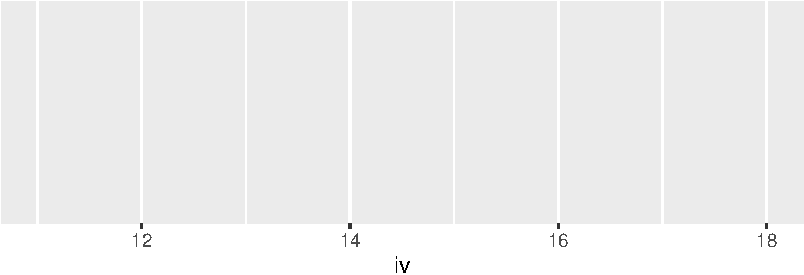
\includegraphics{r_visualization_files/figure-pdf/fig-r-basics-ggplot-02-1.pdf}

}

\caption{\label{fig-r-basics-ggplot-02}}

\end{figure}%

Die Grafik ist marginal interessanter geworden (siehe
Figure~\ref{fig-r-basics-ggplot-02}). Allerdings haben wir jetzt eine
vollständige \(x\)-Achse mit Beschriftung und Einheiten. Im Code haben
wir dazu an das Argument \texttt{mapping} ein \texttt{aes()} Funktion
übergeben, der wir wiederum das Argument \texttt{x} mit dem Namen der
Variable belegt haben, das wir auf die \(x\)-Achse abbilden wollen. Wenn
ihr euch die Hilfe für \texttt{?ggplot()} anschaut, dann seht ihr, das
das zweite Argument sowieso \texttt{mapping} ist, daher können wir uns
die Argumentenbezeichnung auch schenken. Wenn es in \texttt{aes()} ein
\texttt{x} gibt, dann wird es wohl auch ein \texttt{y} geben. Bilden wir
daher die Variable \texttt{dv} aus \texttt{df} auf die \(y\)-Achse ab.

\begin{Shaded}
\begin{Highlighting}[]
\FunctionTok{ggplot}\NormalTok{(df, }\FunctionTok{aes}\NormalTok{(}\AttributeTok{x =}\NormalTok{ iv, }\AttributeTok{y =}\NormalTok{ dv))}
\end{Highlighting}
\end{Shaded}

\begin{figure}[H]

\centering{

\captionsetup{labelsep=none}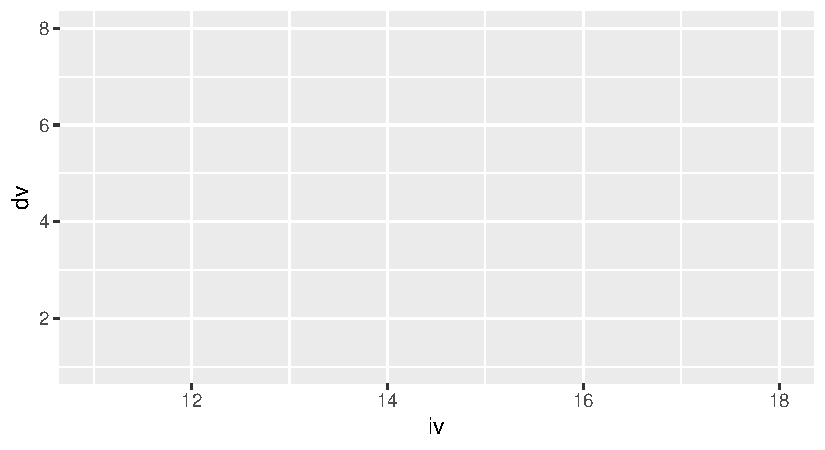
\includegraphics{r_visualization_files/figure-pdf/fig-r-basics-ggplot-03-1.pdf}

}

\caption{\label{fig-r-basics-ggplot-03}}

\end{figure}%

In Figure~\ref{fig-r-basics-ggplot-03} ist jetzt die zweite Achse
erstellt worden. Nur sehen wir noch keine Daten. Wenn wir uns
\texttt{?aes} anschauen, dann sehen wir das \texttt{x} und \texttt{y}
sowieso Argumente 1 und 2 für \texttt{aes()} sind, daher können wir uns
die Bezeichnung wieder sparen. Aber noch mal zurück zu den Abbildungen.
Es gibt nicht nur die beiden Achsen, sondern auch zum Beispiel die Größe
oder Farbe von Objekte. Diese werden aber erst interessant wenn wir
Ebenen mit geometrische Objekte auf definieren.

\subsection{\texorpdfstring{\texttt{geom\_point()}}{geom\_point()}}\label{geom_point}

Fangen mit dem einfachsten geometrischen Objekt an, dem Punkt bzw. den
Punkten. Punkte sind mindestens durch ihre \(x\) und \(y\)-Position, die
Größe und die Farbe gekennzeichnet. Schauen wir uns zunächst einmal nur
die Position an, und lassen die Farbe und die Größe auf den
voreingestellten Werten.

\begin{Shaded}
\begin{Highlighting}[]
\FunctionTok{ggplot}\NormalTok{(df, }\FunctionTok{aes}\NormalTok{(}\AttributeTok{x =}\NormalTok{ dv, }\AttributeTok{y =}\NormalTok{ iv)) }\SpecialCharTok{+}
  \FunctionTok{geom\_point}\NormalTok{()}
\end{Highlighting}
\end{Shaded}

\begin{figure}[H]

\centering{

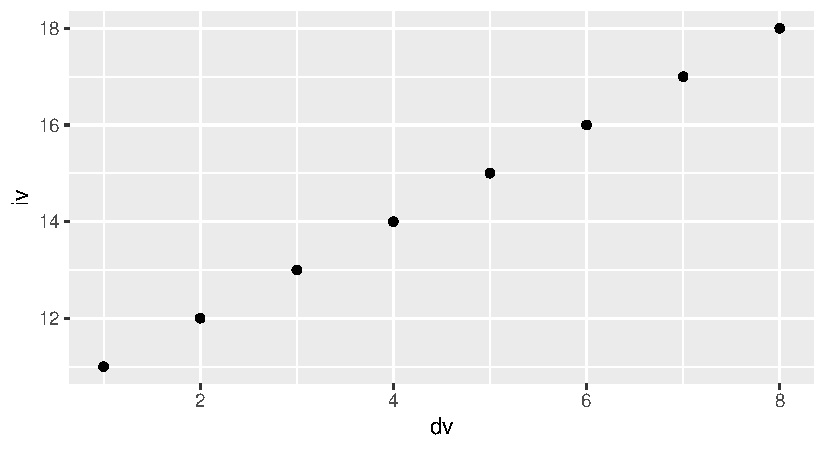
\includegraphics{r_visualization_files/figure-pdf/fig-r-basics-scatterplot-1.pdf}

}

\caption{\label{fig-r-basics-scatterplot}Ein Streudiagramm}

\end{figure}%

In Figure~\ref{fig-r-basics-scatterplot} haben wir ein einfaches
Streudiagramm der Daten erstellt. Schauen wir uns den Code etwas genauer
an. Wir haben eine Funktion \texttt{geom\_point()} verwendet und diese
mittels eines \texttt{+} an \texttt{ggplot()} angehängt. Der erste Teil
des Namens \texttt{geom} zeigt an, das es sich um ein geometrische
Objekt handelt. Im Folgenden werden wir verschiedene Funktionen sehen,
die alle mit dem Kürzel \texttt{geom} beginnen und entsprechend
unterschiedliche Formen haben. Für jedes \texttt{geom} erstellt
\texttt{ggplot()} eine eigene Ebene. Eine mentales Template könnte eine
Folie wie früher bei den Overhead-Projektoren sein. \texttt{ggplot()}
nimmt sich eine leere Folie, legt diese auf die Grafikfolie mit den
Achsen und malt die Punkte an die entsprechende Stelle auf die leere
Folie.

Wie vorhin schon erwähnt führt der folgende kürzere Code zum gleichen
Ergebnis.

\begin{Shaded}
\begin{Highlighting}[]
\FunctionTok{ggplot}\NormalTok{(df, }\FunctionTok{aes}\NormalTok{(dv, iv)) }\SpecialCharTok{+}
  \FunctionTok{geom\_point}\NormalTok{()}
\end{Highlighting}
\end{Shaded}

Diese Schreibweise wird uns im Folgenden immer wieder begegnen. Wenn ihr
euch die Hilfe für \texttt{geom\_point()} anseht, dann stellt ihr fest,
dass \texttt{geom\_point()} tatsächlich eine ganz normale
Wald-und-Wiesen Funktion ist. Das erste Argument an
\texttt{geom\_point()} ist ebenfalls \texttt{mapping}. Daher können wir
das Streudiagramm auch folgendermaßen erstellen.

\begin{Shaded}
\begin{Highlighting}[]
\FunctionTok{ggplot}\NormalTok{(df) }\SpecialCharTok{+}
  \FunctionTok{geom\_point}\NormalTok{(}\FunctionTok{aes}\NormalTok{(dv, iv))}
\end{Highlighting}
\end{Shaded}

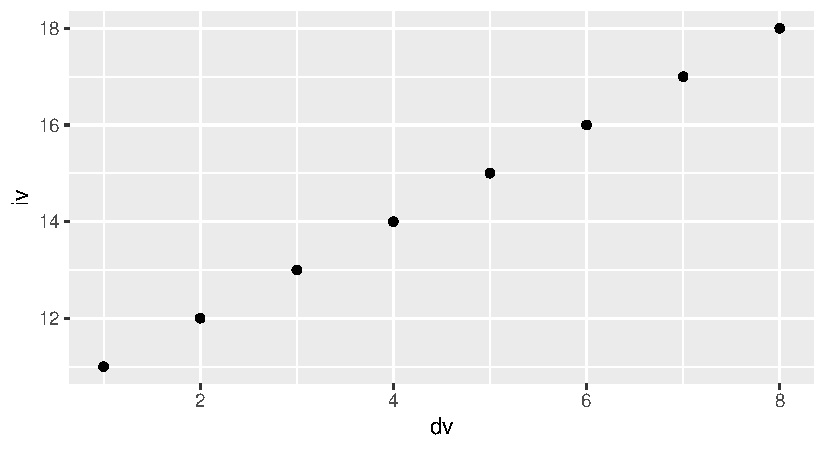
\includegraphics{r_visualization_files/figure-pdf/unnamed-chunk-10-1.pdf}

Der Unterschied zwischen dem Argument \texttt{mapping} in
\texttt{ggplot()} und in \texttt{geom\_point()} besteht darin, dass die
Abbildung im ersten Falle für alle \texttt{geom}s gilt die weiter
angehängt werden, während im zweiten Fall, \texttt{mapping} in
\texttt{geom\_point()} die Abbildung nur für \texttt{geom\_point()}
gilt. Wenn wir gleich mehrere \texttt{geom} aneinanderreihen wird der
Unterschied klarer.

Schauen wir uns als nächste zwei verschiedene Arten an, die Größe für
die Punkte zu bestimmen. Hier gibt es auch wieder zwei Fälle zu
unterscheiden. Einmal die Größe innerhalb von \texttt{aes()} zu
bestimmen oder als Argument zu \texttt{geom\_point()}. Im ersten Fall
können wir dynamisch anhand der zugewiesenen Abbildungsvariable die
Größe verändern, während im zweiten eine Größe für alle Punkte
zugewiesen wird. Innerhalb von \texttt{aes()} können wir den Namen der
Variable nehmen, während dies in \texttt{geom\_point()} nicht möglich
ist, hier müssen wir eine Zahl übergeben.

\begin{Shaded}
\begin{Highlighting}[]
\FunctionTok{ggplot}\NormalTok{(df, }\FunctionTok{aes}\NormalTok{(dv,iv, }\AttributeTok{size=}\NormalTok{dv)) }\SpecialCharTok{+}
\FunctionTok{geom\_point}\NormalTok{()}
\FunctionTok{ggplot}\NormalTok{(df, }\FunctionTok{aes}\NormalTok{(dv, iv)) }\SpecialCharTok{+}
\FunctionTok{geom\_point}\NormalTok{(}\AttributeTok{size=}\DecValTok{4}\NormalTok{)}
\end{Highlighting}
\end{Shaded}

\begin{figure}

\begin{minipage}{0.50\linewidth}

\centering{

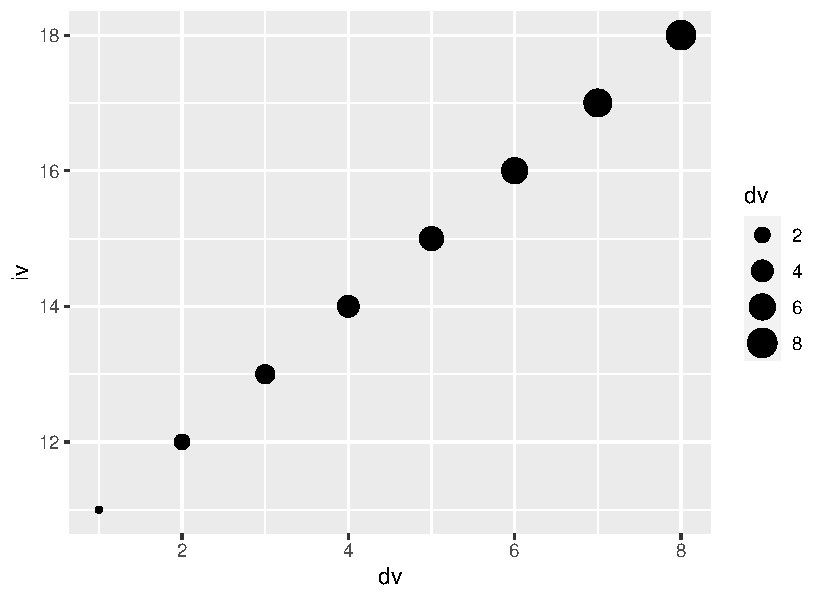
\includegraphics{r_visualization_files/figure-pdf/fig-r-basics-scattersize-1.pdf}

}

\subcaption{\label{fig-r-basics-scattersize-1}Definition in
\texttt{aes()}}

\end{minipage}%
%
\begin{minipage}{0.50\linewidth}

\centering{

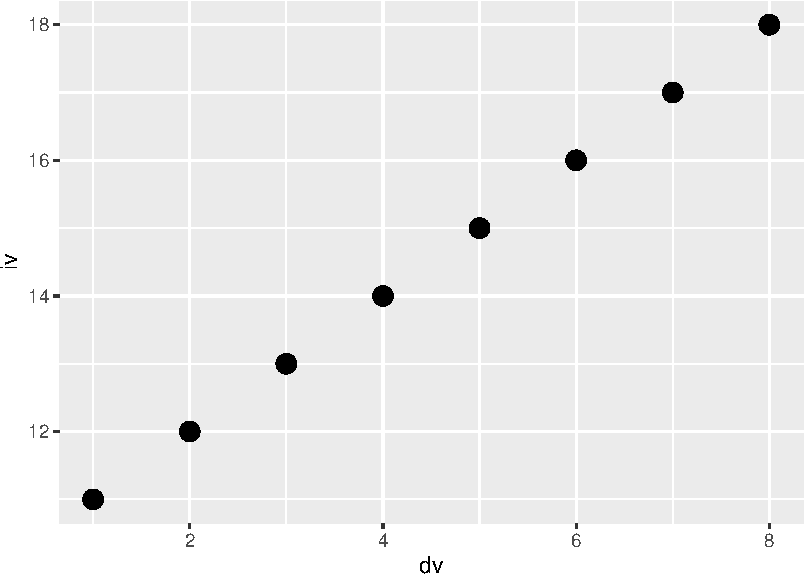
\includegraphics{r_visualization_files/figure-pdf/fig-r-basics-scattersize-2.pdf}

}

\subcaption{\label{fig-r-basics-scattersize-2}Definition in
\texttt{geom\_point()}}

\end{minipage}%

\caption{\label{fig-r-basics-scattersize}Definition der Punktgröße auf
zwei Arten}

\end{figure}%

In Figure~\ref{fig-r-basics-scattersize-1} sehen wir, dass die Größe der
Punkte variiert und \texttt{ggplot()} auch noch eine Legende der Größen
angefügt hat. In Figure~\ref{fig-r-basics-scattersize-2} haben alle
Punkte die gleiche Größe.

Das gleiche Prinzip können wir auch auf die Farbe der Punkte anwenden.

\begin{Shaded}
\begin{Highlighting}[]
\FunctionTok{ggplot}\NormalTok{(df, }\FunctionTok{aes}\NormalTok{(dv,iv, }\AttributeTok{color =}\NormalTok{ team)) }\SpecialCharTok{+}
\FunctionTok{geom\_point}\NormalTok{()}
\FunctionTok{ggplot}\NormalTok{(df, }\FunctionTok{aes}\NormalTok{(dv, iv)) }\SpecialCharTok{+}
\FunctionTok{geom\_point}\NormalTok{(}\AttributeTok{color =} \StringTok{\textquotesingle{}red\textquotesingle{}}\NormalTok{)}
\end{Highlighting}
\end{Shaded}

\begin{figure}

\begin{minipage}{0.50\linewidth}

\centering{

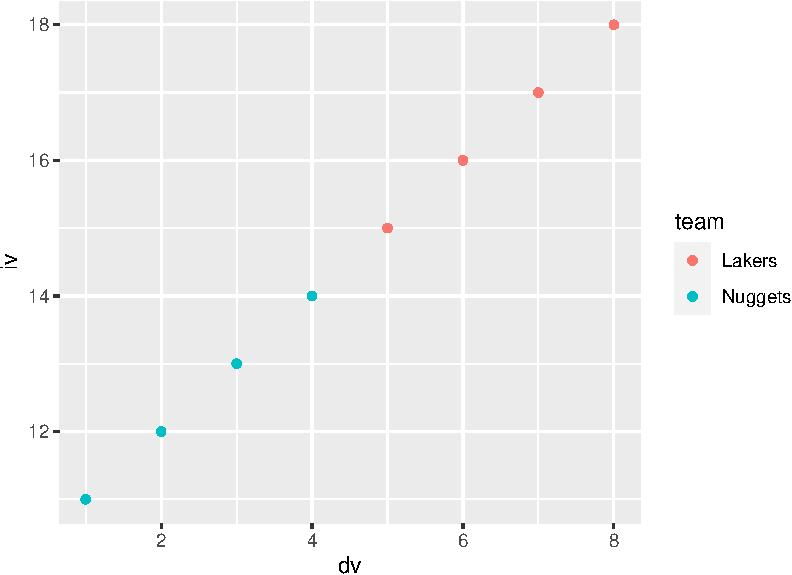
\includegraphics{r_visualization_files/figure-pdf/fig-r-basics-scattercol-1.pdf}

}

\subcaption{\label{fig-r-basics-scattercol-1}Definition in
\texttt{aes()}}

\end{minipage}%
%
\begin{minipage}{0.50\linewidth}

\centering{

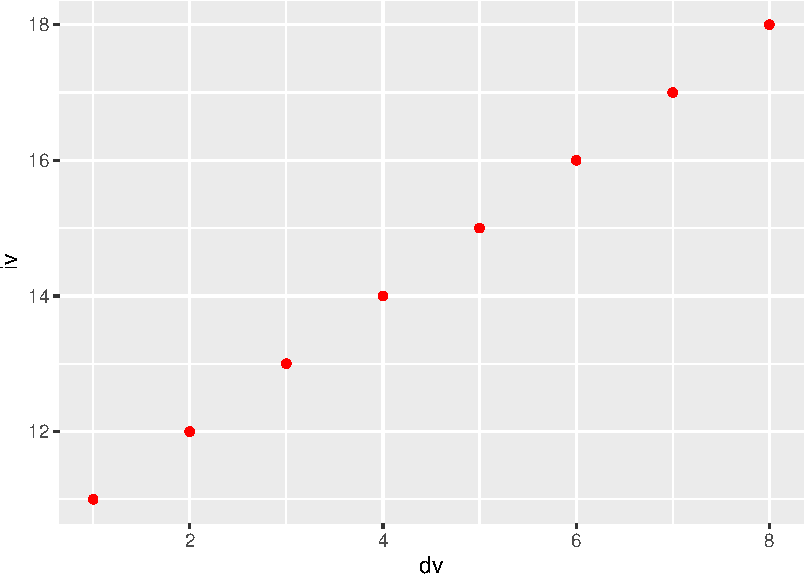
\includegraphics{r_visualization_files/figure-pdf/fig-r-basics-scattercol-2.pdf}

}

\subcaption{\label{fig-r-basics-scattercol-2}Definition in
\texttt{geom\_point()}}

\end{minipage}%

\caption{\label{fig-r-basics-scattercol}Definition der Punktfarbe auf
zwei Arten}

\end{figure}%

Wenn die Farbe in \texttt{aes()} definiert wird, erhalten wir eine
Legende und die Farbe wird anhand der Variable bestimmt (siehe
Figure~\ref{fig-r-basics-scattercol-1}), während bei der Definition als
Argument zu \texttt{geom\_point()} alle Punkte die gleiche Farbe
bekommen (siehe Figure~\ref{fig-r-basics-scattercol-2}).

Natürlich können wir auch gleichzeitig die Farbei und die Größe
bestimmen.

\begin{Shaded}
\begin{Highlighting}[]
\FunctionTok{ggplot}\NormalTok{(df, }\FunctionTok{aes}\NormalTok{(dv,iv, }\AttributeTok{size =}\NormalTok{ dv, }\AttributeTok{color =}\NormalTok{ team)) }\SpecialCharTok{+}
\FunctionTok{geom\_point}\NormalTok{()}
\FunctionTok{ggplot}\NormalTok{(df, }\FunctionTok{aes}\NormalTok{(dv, iv)) }\SpecialCharTok{+}
\FunctionTok{geom\_point}\NormalTok{(}\AttributeTok{size =} \DecValTok{4}\NormalTok{, }\AttributeTok{color =} \StringTok{\textquotesingle{}red\textquotesingle{}}\NormalTok{)}
\end{Highlighting}
\end{Shaded}

\begin{figure}

\begin{minipage}{0.50\linewidth}

\centering{

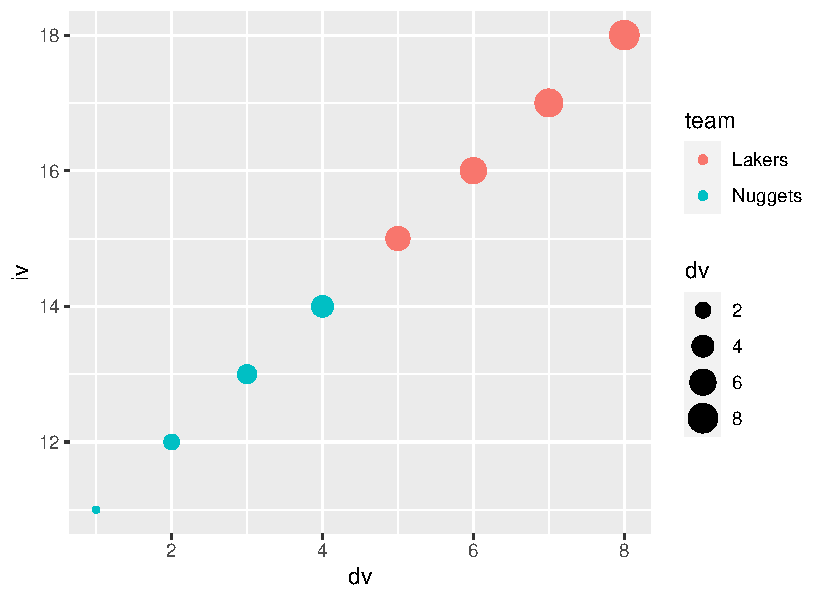
\includegraphics{r_visualization_files/figure-pdf/fig-r-basics-scattercolsize-1.pdf}

}

\subcaption{\label{fig-r-basics-scattercolsize-1}Definition in
\texttt{aes()}}

\end{minipage}%
%
\begin{minipage}{0.50\linewidth}

\centering{

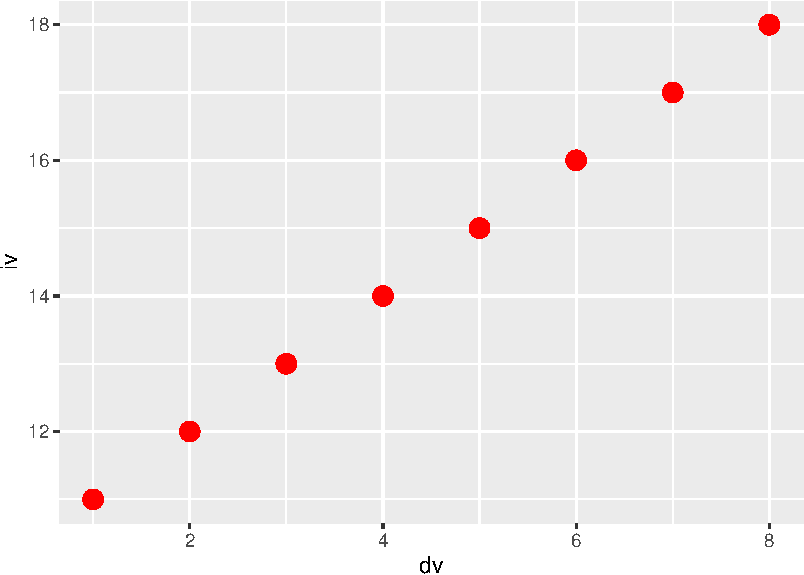
\includegraphics{r_visualization_files/figure-pdf/fig-r-basics-scattercolsize-2.pdf}

}

\subcaption{\label{fig-r-basics-scattercolsize-2}Definition in
\texttt{geom\_point()}}

\end{minipage}%

\caption{\label{fig-r-basics-scattercolsize}Definition der Punktfarbe
und Punktgröße auf zwei Arten}

\end{figure}%

\subsection{\texorpdfstring{\texttt{geom\_line()}}{geom\_line()}}\label{geom_line}

Schauen wir uns als nächstes \texttt{geom\_line()} an. Wie der Name
vermuten lässt, können wir mit diesem \texttt{geom} Linien erstellen.
Linen werden zwischen aufeinanderfolgenden Punkten die eine
\((x,y)\)-Position haben gezogen. Daher sind die gleichen Abbildungen
wie bei den Punkten möglich.

\begin{Shaded}
\begin{Highlighting}[]
\FunctionTok{ggplot}\NormalTok{(df, }\FunctionTok{aes}\NormalTok{(iv,dv)) }\SpecialCharTok{+}
  \FunctionTok{geom\_line}\NormalTok{()}
\end{Highlighting}
\end{Shaded}

\begin{figure}[H]

\centering{

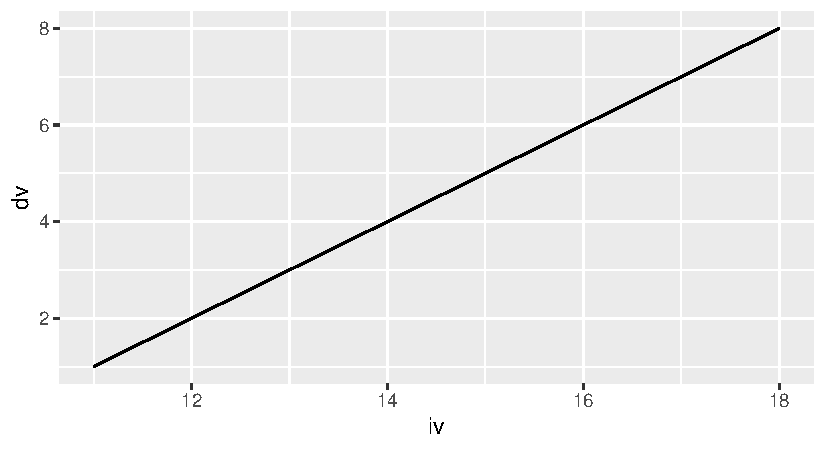
\includegraphics{r_visualization_files/figure-pdf/fig-r-basics-line-01-1.pdf}

}

\caption{\label{fig-r-basics-line-01}Linendiagramm}

\end{figure}%

Wenn wir zwei unterschiedlichen Linien für die Teams erstellen wollen,
dann können wir das zum Beispiel über die Farbe steuern.

\begin{Shaded}
\begin{Highlighting}[]
\FunctionTok{ggplot}\NormalTok{(df, }\FunctionTok{aes}\NormalTok{(iv, dv, }\AttributeTok{color =}\NormalTok{ team)) }\SpecialCharTok{+}
  \FunctionTok{geom\_line}\NormalTok{()}
\end{Highlighting}
\end{Shaded}

\begin{figure}[H]

\centering{

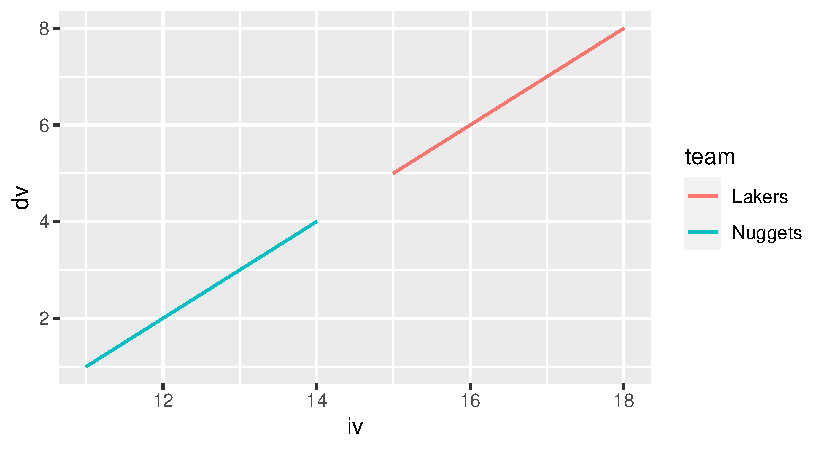
\includegraphics{r_visualization_files/figure-pdf/fig-r-basics-line-02-1.pdf}

}

\caption{\label{fig-r-basics-line-02}Liniendiagramm unterteilt nach
Team}

\end{figure}%

Jetzt fehlt in Figure~\ref{fig-r-basics-line-02} das Verbindungsstück
zwischen den beiden Punkten das in Figure~\ref{fig-r-basics-line-01}
noch vorhanden war, da \texttt{ggplot()} den Datensatz in zwei
Teildatensätze unterteilt.

Wie oben schon angedeutet können wir mehrere \texttt{geom} miteinander
kombinieren.

\begin{Shaded}
\begin{Highlighting}[]
\FunctionTok{ggplot}\NormalTok{(df, }\FunctionTok{aes}\NormalTok{(iv, dv)) }\SpecialCharTok{+}
  \FunctionTok{geom\_line}\NormalTok{() }\SpecialCharTok{+}
  \FunctionTok{geom\_point}\NormalTok{()}
\end{Highlighting}
\end{Shaded}

\begin{figure}[H]

\centering{

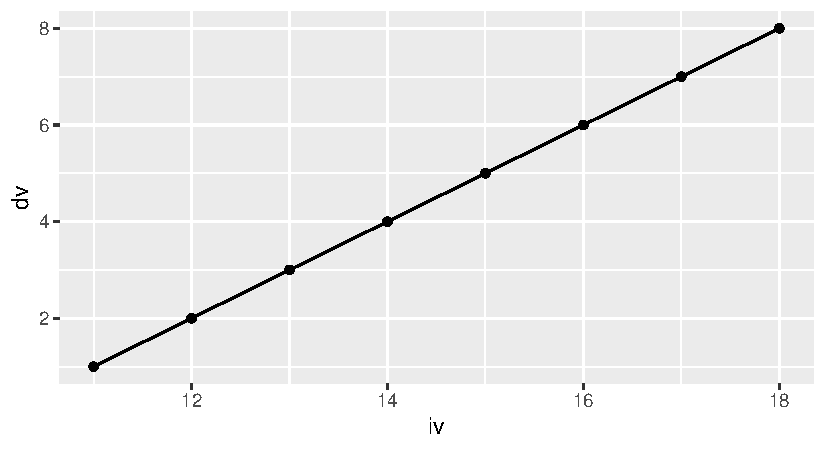
\includegraphics{r_visualization_files/figure-pdf/fig-r-basics-line-03-1.pdf}

}

\caption{\label{fig-r-basics-line-03}Ein kombiniertes Linien und
Streudiagramm}

\end{figure}%

Die Reihenfolge spielt dabei eine Rolle, \texttt{geom}s die später
dazugefügt werden, liegen oberhalb von \texttt{geom}s die früher
definiert wurden.

\begin{Shaded}
\begin{Highlighting}[]
\FunctionTok{ggplot}\NormalTok{(df, }\FunctionTok{aes}\NormalTok{(iv, dv)) }\SpecialCharTok{+}
  \FunctionTok{geom\_point}\NormalTok{(}\AttributeTok{color =} \StringTok{\textquotesingle{}red\textquotesingle{}}\NormalTok{, }\AttributeTok{size =} \DecValTok{4}\NormalTok{) }\SpecialCharTok{+}
  \FunctionTok{geom\_line}\NormalTok{()}
\FunctionTok{ggplot}\NormalTok{(df, }\FunctionTok{aes}\NormalTok{(iv, dv)) }\SpecialCharTok{+}
  \FunctionTok{geom\_line}\NormalTok{() }\SpecialCharTok{+} 
  \FunctionTok{geom\_point}\NormalTok{(}\AttributeTok{color =} \StringTok{\textquotesingle{}red\textquotesingle{}}\NormalTok{, }\AttributeTok{size =} \DecValTok{4}\NormalTok{) }
\end{Highlighting}
\end{Shaded}

\begin{figure}

\begin{minipage}{0.50\linewidth}

\centering{

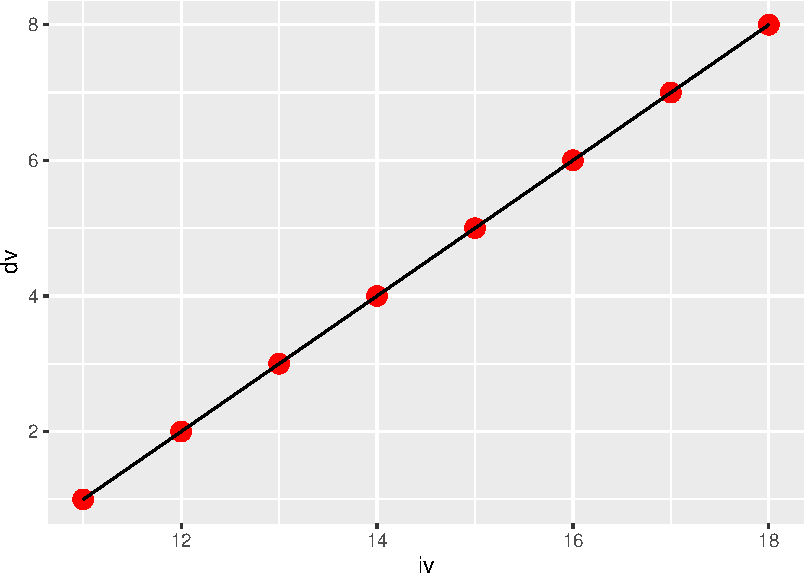
\includegraphics{r_visualization_files/figure-pdf/fig-r-basics-line-04-1.pdf}

}

\subcaption{\label{fig-r-basics-line-04-1}\texttt{geom\_point()\ \ vor}geom\_line()`}

\end{minipage}%
%
\begin{minipage}{0.50\linewidth}

\centering{

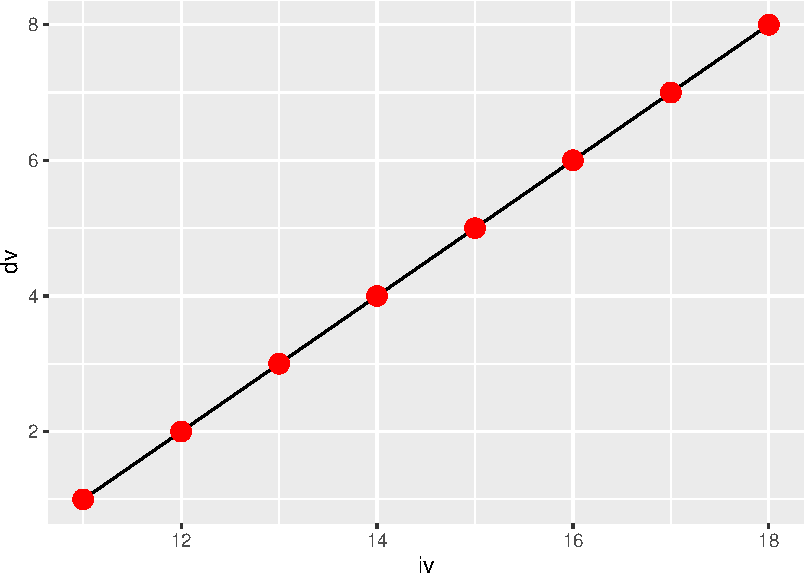
\includegraphics{r_visualization_files/figure-pdf/fig-r-basics-line-04-2.pdf}

}

\subcaption{\label{fig-r-basics-line-04-2}\texttt{geom\_line()\ \ vor}geom\_point()`}

\end{minipage}%

\caption{\label{fig-r-basics-line-04}Einfluss der Reihenfolge von
\texttt{geom}s}

\end{figure}%

In Figure~\ref{fig-r-basics-line-04-1} sehen wir, dass die Linien die
Punkte durchschneiden, da sie oberhalb liegen, während in
Figure~\ref{fig-r-basics-line-04-2} die Linien hinter den Punkten
liegen.

Vielleicht ist es euch schon aufgefallen, das wir in den letzten beiden
Beispielen den Mechanismus verwendet haben, dass die Abbilung in
\texttt{ggplot()} definiert wurden und dann für bei beide \texttt{geom}s
\texttt{geom\_point()} und \texttt{geom\_line()} angewendet wurden. Wenn
wir die Abbildung nur ein \texttt{geom\_point()} definiert hätten, dann
würde \texttt{geom\_point()} meckern, das es nicht weiß wo es die Punkte
hinsetzen soll.

\begin{Shaded}
\begin{Highlighting}[]
\FunctionTok{ggplot}\NormalTok{(df)  }\SpecialCharTok{+}
  \FunctionTok{geom\_line}\NormalTok{(}\FunctionTok{aes}\NormalTok{(iv, dv)) }\SpecialCharTok{+} 
  \FunctionTok{geom\_point}\NormalTok{() }
\end{Highlighting}
\end{Shaded}

\begin{verbatim}
Error in `geom_point()`:
! Problem while setting up geom.
i Error occurred in the 2nd layer.
Caused by error in `compute_geom_1()`:
! `geom_point()` requires the following missing aesthetics: x and y
\end{verbatim}

Nachdem wir jetzt schon die Grundprinzipien kennengelernt haben, schauen
wir uns die nächsten \texttt{geom}s etwas kürze an.

\subsection{\texorpdfstring{\texttt{geom\_boxplot()}}{geom\_boxplot()}}\label{geom_boxplot}

Der Boxplot als eine praktische Art der Visualisierung sollte natürlich
auch nicht fehlen und hat daher auch ein eigenes \texttt{geom} spendiert
bekommen. Hier ist zu beachten, dass die Abbildung auf die \(x\)-Achse
üblichweise nicht numerisch sondern entweder nominal oder ordinal ist.
In der Praxis können auch Zeichenketten verwendet werden, die dann als
Faktor interpretiert werden.

\begin{Shaded}
\begin{Highlighting}[]
\FunctionTok{ggplot}\NormalTok{(df, }\FunctionTok{aes}\NormalTok{(team, dv)) }\SpecialCharTok{+}
  \FunctionTok{geom\_boxplot}\NormalTok{()}
\end{Highlighting}
\end{Shaded}

\begin{figure}[H]

\centering{

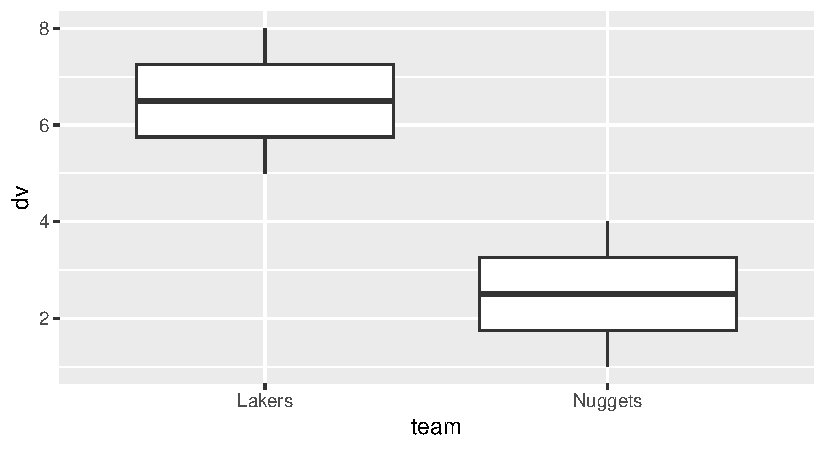
\includegraphics{r_visualization_files/figure-pdf/fig-r-basics-boxplot-1.pdf}

}

\caption{\label{fig-r-basics-boxplot}Ein Boxplot mit
\texttt{geom\_boxplot()}.}

\end{figure}%

Wir können wieder mehrere Abbildungen kombinieren und zum Beispiel
getrennte Boxplots für die Teams und die Gruppen erstellen.

\begin{Shaded}
\begin{Highlighting}[]
\FunctionTok{ggplot}\NormalTok{(df, }\FunctionTok{aes}\NormalTok{(team, dv, }\AttributeTok{fill=}\NormalTok{group)) }\SpecialCharTok{+}
  \FunctionTok{geom\_boxplot}\NormalTok{()}
\end{Highlighting}
\end{Shaded}

\begin{figure}[H]

\centering{

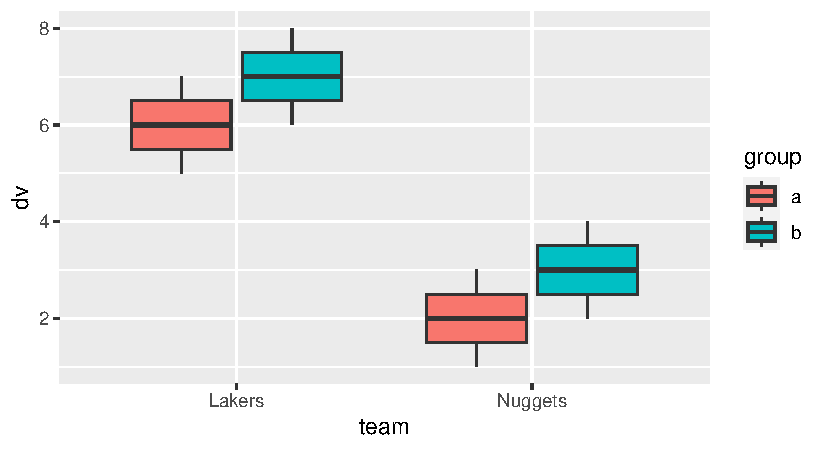
\includegraphics{r_visualization_files/figure-pdf/fig-r-basics-boxplot-2-1.pdf}

}

\caption{\label{fig-r-basics-boxplot-2}Getrennte Boxplots nach Team und
Gruppe.}

\end{figure}%

\subsection{\texorpdfstring{\texttt{geom\_col()}}{geom\_col()}}\label{geom_col}

Die nächste Art von Visualisierung sind Säulendiagramme. Hier müssen wir
allerdings etwas Vorarbeit leisten. Bei Säulendiagrammen wird in den
meisten Fällen der Mittelwert dargestellt. Daher müssen wir den
Mittelwert zunächste berechnen.

\begin{Shaded}
\begin{Highlighting}[]
\NormalTok{df\_team }\OtherTok{\textless{}{-}}\NormalTok{ df }\SpecialCharTok{|\textgreater{}} 
  \FunctionTok{group\_by}\NormalTok{(team) }\SpecialCharTok{|\textgreater{}} 
  \FunctionTok{summarize}\NormalTok{(}\AttributeTok{m =} \FunctionTok{mean}\NormalTok{(dv), }\AttributeTok{sd =} \FunctionTok{sd}\NormalTok{(dv))}
\end{Highlighting}
\end{Shaded}

\begin{longtable}[]{@{}lrr@{}}
\toprule\noalign{}
team & m & sd \\
\midrule\noalign{}
\endhead
\bottomrule\noalign{}
\endlastfoot
Lakers & 6.5 & 1.29 \\
Nuggets & 2.5 & 1.29 \\
\end{longtable}

Wir haben gleich auch noch die Standardabweichungen berechnet, da wir
die gleich benötigen werden. Säulendiagramme können mit
\texttt{geom\_col()} erstellt werden. Wie bei \texttt{geom\_boxplot()}
sollte die \(x\)-Skala nominal sein.

\begin{Shaded}
\begin{Highlighting}[]
\FunctionTok{ggplot}\NormalTok{(df\_team, }\FunctionTok{aes}\NormalTok{(team, m)) }\SpecialCharTok{+}
  \FunctionTok{geom\_col}\NormalTok{()}
\end{Highlighting}
\end{Shaded}

\begin{figure}[H]

\centering{

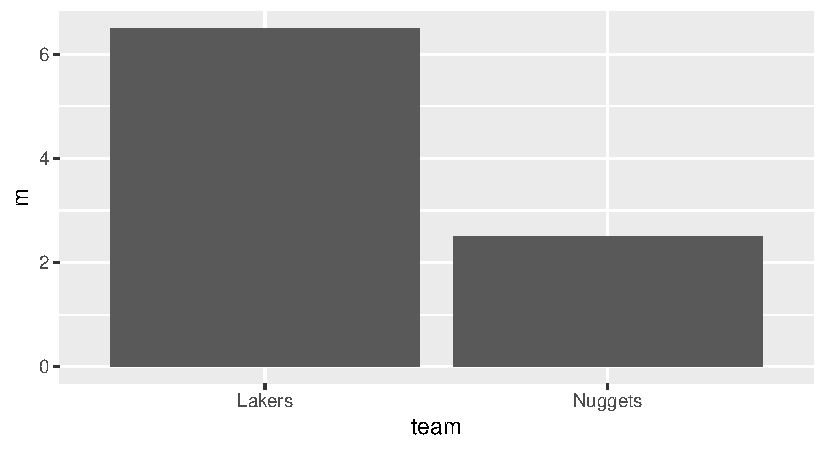
\includegraphics{r_visualization_files/figure-pdf/fig-r-basics-col-01-1.pdf}

}

\caption{\label{fig-r-basics-col-01}Ein Säulendiagramm mit
\texttt{geom\_col()}.}

\end{figure}%

So weit so gut, aber keine Darstellung des Mittelwerts ohne eine
Darstellung der Streuung. Dazu benötigen wir allerdings ein weiteres
\texttt{geom}.

\subsection{\texorpdfstring{\texttt{geom\_errorbar()}}{geom\_errorbar()}}\label{geom_errorbar}

Um die Streuung in einem Säulendiagramm darzustellen, verwenden wir
\texttt{geom\_errorbar()}. Hier kommen endlich einmal zwei neue
Abbildungen ins Spiel. \texttt{ymin} bestimmt das untere Ende des
Fehlerbalkens, während \texttt{ymax} das obere Ende bestimmt. D.h. die
Fehlerbalken müssen nicht unbedingt in beide Richtungen gleich lang
sein.

\begin{Shaded}
\begin{Highlighting}[]
\FunctionTok{ggplot}\NormalTok{(df\_team, }\FunctionTok{aes}\NormalTok{(team, m)) }\SpecialCharTok{+}
  \FunctionTok{geom\_col}\NormalTok{() }\SpecialCharTok{+}
  \FunctionTok{geom\_errorbar}\NormalTok{(}\FunctionTok{aes}\NormalTok{(}\AttributeTok{ymin =}\NormalTok{ m }\SpecialCharTok{{-}}\NormalTok{ sd, }\AttributeTok{ymax =}\NormalTok{ m }\SpecialCharTok{+}\NormalTok{ sd))}
\end{Highlighting}
\end{Shaded}

\begin{figure}[H]

\centering{

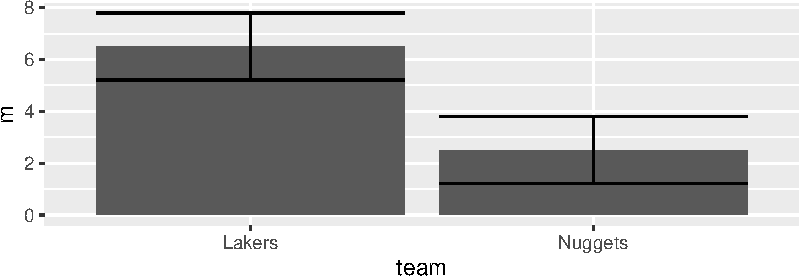
\includegraphics{r_visualization_files/figure-pdf/fig-r-basics-col-02-1.pdf}

}

\caption{\label{fig-r-basics-col-02}Ein Säulendiagram mit
\texttt{geom\_col()}.}

\end{figure}%

In Figure~\ref{fig-r-basics-col-02} können wir nun die Fehlerbalken
sehen. Allerdings sehen die Fehlerbalken noch nicht besonders schön aus,
da sie relativ breit sind. Mit dem Argument \texttt{width} können wir
spezifieren wie breit die Hüte sein sollen. Mit dem Parameter
\texttt{linewidth} können wir zusätzlich noch die Linienbreite
bestimmen. Passen wir auch gleich noch die Farbe etwas an.

\begin{Shaded}
\begin{Highlighting}[]
\FunctionTok{ggplot}\NormalTok{(df\_team, }\FunctionTok{aes}\NormalTok{(team, m)) }\SpecialCharTok{+}
  \FunctionTok{geom\_col}\NormalTok{() }\SpecialCharTok{+}
  \FunctionTok{geom\_errorbar}\NormalTok{(}\FunctionTok{aes}\NormalTok{(}\AttributeTok{ymin =}\NormalTok{ m }\SpecialCharTok{{-}}\NormalTok{ sd, }\AttributeTok{ymax =}\NormalTok{ m }\SpecialCharTok{+}\NormalTok{ sd),}
                \AttributeTok{width =} \FloatTok{0.3}\NormalTok{,}
                \AttributeTok{color =} \StringTok{\textquotesingle{}red\textquotesingle{}}\NormalTok{,}
                \AttributeTok{linewidth =} \FloatTok{1.5}\NormalTok{)}
\end{Highlighting}
\end{Shaded}

\begin{figure}[H]

\centering{

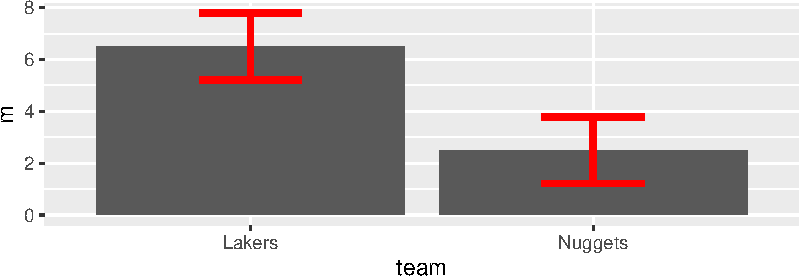
\includegraphics{r_visualization_files/figure-pdf/fig-r-basics-col-03-1.pdf}

}

\caption{\label{fig-r-basics-col-03}Ein Säulendiagram mit
\texttt{geom\_col()}.}

\end{figure}%

Ein Problem mit den Fehlerbalken mit \texttt{geom\_errorbar()} entsteht
wenn es mehrere Werte für jeden \(x\)-Wert gibt. In der
Standardeinstellung werden die Werte aufeinander gesetzt (stacked).
Erstellen wir uns erst einmal einen passenden Datensatz.

\begin{Shaded}
\begin{Highlighting}[]
\NormalTok{df\_tg }\OtherTok{\textless{}{-}}\NormalTok{ df }\SpecialCharTok{|\textgreater{}} \FunctionTok{group\_by}\NormalTok{(team, group) }\SpecialCharTok{|\textgreater{}} \FunctionTok{summarize}\NormalTok{(}\AttributeTok{dv\_bar =} \FunctionTok{mean}\NormalTok{(dv), }\AttributeTok{dv\_sd =} \FunctionTok{sd}\NormalTok{(dv))}
\end{Highlighting}
\end{Shaded}

\begin{longtable}[]{@{}llrr@{}}
\toprule\noalign{}
team & group & dv\_bar & dv\_sd \\
\midrule\noalign{}
\endhead
\bottomrule\noalign{}
\endlastfoot
Lakers & a & 6 & 1.414 \\
Lakers & b & 7 & 1.414 \\
Nuggets & a & 2 & 1.414 \\
Nuggets & b & 3 & 1.414 \\
\end{longtable}

Schauen wir uns erst einmal nur die Säulen an.

\begin{Shaded}
\begin{Highlighting}[]
\FunctionTok{ggplot}\NormalTok{(df\_tg, }\FunctionTok{aes}\NormalTok{(team, dv\_bar, }\AttributeTok{fill =}\NormalTok{ group)) }\SpecialCharTok{+}
  \FunctionTok{geom\_col}\NormalTok{()}
\end{Highlighting}
\end{Shaded}

\begin{figure}[H]

\centering{

\captionsetup{labelsep=none}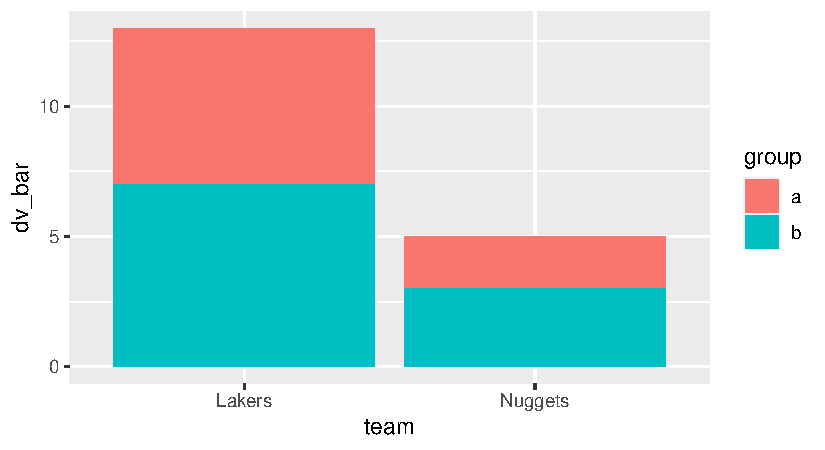
\includegraphics{r_visualization_files/figure-pdf/fig-r-basics-col-04-1.pdf}

}

\caption{\label{fig-r-basics-col-04}}

\end{figure}%

In Figure~\ref{fig-r-basics-col-04} sind die Mehrfachwerte
aufeinandergestapelt. Dies ist in den seltensten Fällen die
Darstellungsart die wir wirklich wollen, sondern in den meisten Fällen
wollen wir die Säulen nebeneinander angezeigt bekommen. Wir können dies
erreichen indem wir das Argument \texttt{position} mit dem Argument
\texttt{"dodge"} in \texttt{geom\_col()} verwenden.

\begin{Shaded}
\begin{Highlighting}[]
\FunctionTok{ggplot}\NormalTok{(df\_tg, }\FunctionTok{aes}\NormalTok{(team, dv\_bar, }\AttributeTok{fill =}\NormalTok{ group)) }\SpecialCharTok{+}
  \FunctionTok{geom\_col}\NormalTok{(}\AttributeTok{position =} \StringTok{\textquotesingle{}dodge\textquotesingle{}}\NormalTok{)}
\end{Highlighting}
\end{Shaded}

\begin{figure}[H]

\centering{

\captionsetup{labelsep=none}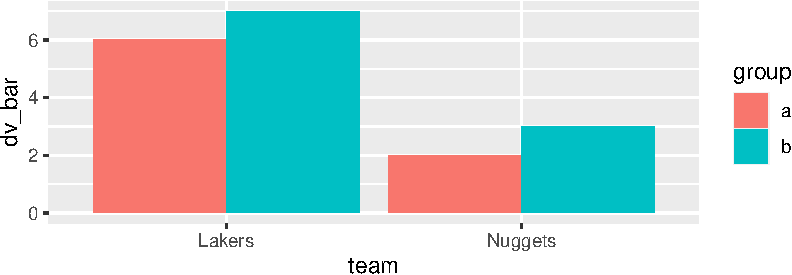
\includegraphics{r_visualization_files/figure-pdf/fig-r-basics-col-05-1.pdf}

}

\caption{\label{fig-r-basics-col-05}}

\end{figure}%

Figure~\ref{fig-r-basics-col-05} sind schon besser aus. Die Säulen sind
nebeneinander dargestellt jeweils für einen \(x\)-Wert. Es entsteht nun
allerdings ein Problem wenn wir die Fehlerbalken dazufügen.

\begin{Shaded}
\begin{Highlighting}[]
\FunctionTok{ggplot}\NormalTok{(df\_tg, }\FunctionTok{aes}\NormalTok{(team, dv\_bar, }\AttributeTok{fill =}\NormalTok{ group)) }\SpecialCharTok{+}
  \FunctionTok{geom\_col}\NormalTok{(}\AttributeTok{position =} \StringTok{\textquotesingle{}dodge\textquotesingle{}}\NormalTok{) }\SpecialCharTok{+}
  \FunctionTok{geom\_errorbar}\NormalTok{(}\FunctionTok{aes}\NormalTok{(}\AttributeTok{ymin =}\NormalTok{ dv\_bar }\SpecialCharTok{{-}}\NormalTok{ dv\_sd, }\AttributeTok{ymax =}\NormalTok{ dv\_bar }\SpecialCharTok{+}\NormalTok{ dv\_sd))}
\end{Highlighting}
\end{Shaded}

\begin{figure}[H]

\centering{

\captionsetup{labelsep=none}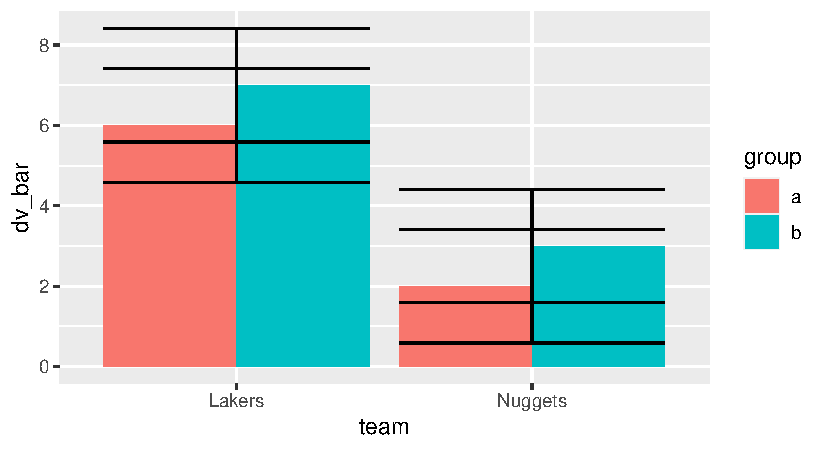
\includegraphics{r_visualization_files/figure-pdf/fig-r-basics-col-06-1.pdf}

}

\caption{\label{fig-r-basics-col-06}}

\end{figure}%

Die Fehlerbalken in Figure~\ref{fig-r-basics-col-06} sind beide in der
Mitte der \(x\)-Werte plaziert und nicht zusammen mit den Säulen
verrückt. Um die Fehlerbalken ebenfalls zu verrücken müssen wir in
\texttt{geom\_errorbar()} ebenfalls den Parameter \texttt{position} mit
dem Argument \texttt{"dodge"} verwenden.

\begin{Shaded}
\begin{Highlighting}[]
\FunctionTok{ggplot}\NormalTok{(df\_tg, }\FunctionTok{aes}\NormalTok{(team, dv\_bar, }\AttributeTok{fill =}\NormalTok{ group)) }\SpecialCharTok{+}
  \FunctionTok{geom\_col}\NormalTok{(}\AttributeTok{position =} \StringTok{\textquotesingle{}dodge\textquotesingle{}}\NormalTok{) }\SpecialCharTok{+}
  \FunctionTok{geom\_errorbar}\NormalTok{(}\FunctionTok{aes}\NormalTok{(}\AttributeTok{ymin =}\NormalTok{ dv\_bar }\SpecialCharTok{{-}}\NormalTok{ dv\_sd, }\AttributeTok{ymax =}\NormalTok{ dv\_bar }\SpecialCharTok{+}\NormalTok{ dv\_sd),}
                \AttributeTok{position =} \StringTok{\textquotesingle{}dodge\textquotesingle{}}\NormalTok{)}
\end{Highlighting}
\end{Shaded}

\begin{figure}[H]

\centering{

\captionsetup{labelsep=none}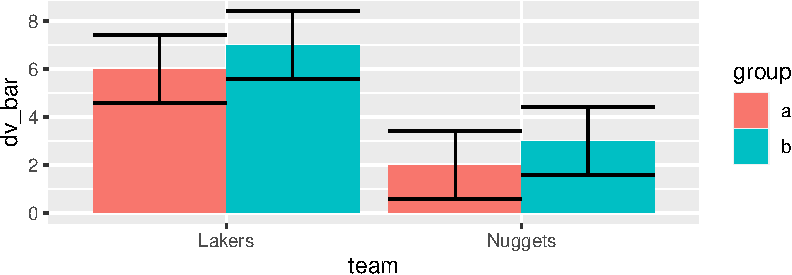
\includegraphics{r_visualization_files/figure-pdf/fig-r-basics-col-07-1.pdf}

}

\caption{\label{fig-r-basics-col-07}}

\end{figure}%

Figure~\ref{fig-r-basics-col-07} kommt schon wieder dem näher was wir
uns vorgestellt haben. Allerdings nur solange wie die Breite mit
\texttt{width} nicht verändern.

\begin{Shaded}
\begin{Highlighting}[]
\FunctionTok{ggplot}\NormalTok{(df\_tg, }\FunctionTok{aes}\NormalTok{(team, dv\_bar, }\AttributeTok{fill =}\NormalTok{ group)) }\SpecialCharTok{+}
  \FunctionTok{geom\_col}\NormalTok{(}\AttributeTok{position =} \StringTok{\textquotesingle{}dodge\textquotesingle{}}\NormalTok{) }\SpecialCharTok{+}
  \FunctionTok{geom\_errorbar}\NormalTok{(}\FunctionTok{aes}\NormalTok{(}\AttributeTok{ymin =}\NormalTok{ dv\_bar }\SpecialCharTok{{-}}\NormalTok{ dv\_sd, }\AttributeTok{ymax =}\NormalTok{ dv\_bar }\SpecialCharTok{+}\NormalTok{ dv\_sd),}
                \AttributeTok{position =} \StringTok{\textquotesingle{}dodge\textquotesingle{}}\NormalTok{,}
                \AttributeTok{width=}\NormalTok{.}\DecValTok{7}\NormalTok{)}
\end{Highlighting}
\end{Shaded}

\begin{figure}[H]

\centering{

\captionsetup{labelsep=none}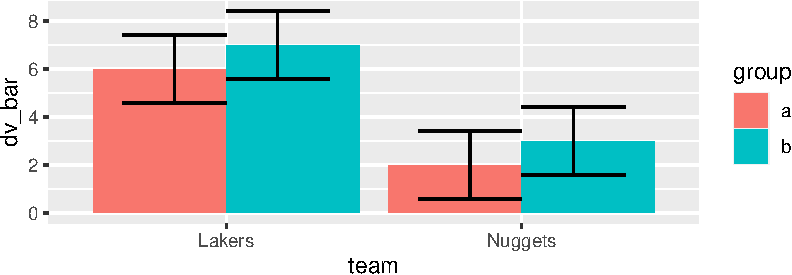
\includegraphics{r_visualization_files/figure-pdf/fig-r-basics-col-08-1.pdf}

}

\caption{\label{fig-r-basics-col-08}}

\end{figure}%

Wie lässt sich Figure~\ref{fig-r-basics-col-08} erklären.
\texttt{ggplot()} berechnet zunächst die Breite des \texttt{geom}s. In
diesem Fall haben wir die Breite für die Fehlerbalken selbst angegeben
mit \texttt{width\ =\ .7}. D.h. Die Fehlerbalken haben die Breite
\(0.7\) graphische Einheiten. Durch den Parameter \texttt{"dodge"} an
\texttt{position} werden die Fehlerbalkennebeneinander dargestellt und
entsprechend der Breite gegeneinander verschoben, so dass keine
Überlappung zustandekommt. Die Säulen gegen die die Fehlerbalken
zentrierte werden sollen sind aber breiter. Standardmäßig weist
\texttt{ggplot()} denen eine Breite von \(0.9\) graphischen Einheiten
zu. Dies bietet dann auch schon die Lösung. \texttt{geom\_errorbar()}
muss die Information bekommen, dass die Fehlerbalken weiter
gegeneinander verschoben werden sollen. Dazu gibt es die Funktion
\texttt{position\_dodge()} mit dem Argument \texttt{width}. Dies kann
verwendet werden um die Verschiebung um einen anderen Faktor als die
Breite des \texttt{geom}s durchzuführen. Für das vorliegende Problem
verwenden wir daher \texttt{position\_dodge(width\ =\ .9)}.

\begin{Shaded}
\begin{Highlighting}[]
\FunctionTok{ggplot}\NormalTok{(df\_tg, }\FunctionTok{aes}\NormalTok{(team, dv\_bar, }\AttributeTok{fill =}\NormalTok{ group)) }\SpecialCharTok{+}
  \FunctionTok{geom\_col}\NormalTok{(}\AttributeTok{position =} \StringTok{\textquotesingle{}dodge\textquotesingle{}}\NormalTok{) }\SpecialCharTok{+}
  \FunctionTok{geom\_errorbar}\NormalTok{(}\FunctionTok{aes}\NormalTok{(}\AttributeTok{ymin =}\NormalTok{ dv\_bar }\SpecialCharTok{{-}}\NormalTok{ dv\_sd, }\AttributeTok{ymax =}\NormalTok{ dv\_bar }\SpecialCharTok{+}\NormalTok{ dv\_sd),}
                \AttributeTok{position =} \FunctionTok{position\_dodge}\NormalTok{(}\AttributeTok{width =}\NormalTok{ .}\DecValTok{9}\NormalTok{), }
                \AttributeTok{width=}\NormalTok{.}\DecValTok{7}\NormalTok{)}
\end{Highlighting}
\end{Shaded}

\begin{figure}[H]

\centering{

\captionsetup{labelsep=none}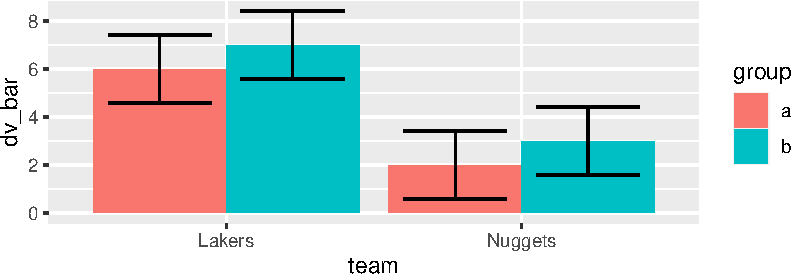
\includegraphics{r_visualization_files/figure-pdf/fig-r-basics-col-09-1.pdf}

}

\caption{\label{fig-r-basics-col-09}}

\end{figure}%

Würden wir die Breite der Säulen selbst spezifieren, dann würden die
Fehlerbalken wieder nicht an der richtigen Position sitzen da die
Verschiebung gegeneinander zu groß ist (siehe
Figure~\ref{fig-r-basics-col-10}).

\begin{Shaded}
\begin{Highlighting}[]
\FunctionTok{ggplot}\NormalTok{(df\_tg, }\FunctionTok{aes}\NormalTok{(team, dv\_bar, }\AttributeTok{fill =}\NormalTok{ group)) }\SpecialCharTok{+}
  \FunctionTok{geom\_col}\NormalTok{(}\AttributeTok{position =} \StringTok{\textquotesingle{}dodge\textquotesingle{}}\NormalTok{, }\AttributeTok{width =} \FloatTok{0.5}\NormalTok{) }\SpecialCharTok{+}
  \FunctionTok{geom\_errorbar}\NormalTok{(}\FunctionTok{aes}\NormalTok{(}\AttributeTok{ymin =}\NormalTok{ dv\_bar }\SpecialCharTok{{-}}\NormalTok{ dv\_sd, }\AttributeTok{ymax =}\NormalTok{ dv\_bar }\SpecialCharTok{+}\NormalTok{ dv\_sd),}
                \AttributeTok{position =} \FunctionTok{position\_dodge}\NormalTok{(}\AttributeTok{width =}\NormalTok{ .}\DecValTok{9}\NormalTok{), }
                \AttributeTok{width=}\NormalTok{.}\DecValTok{7}\NormalTok{)}
\end{Highlighting}
\end{Shaded}

\begin{figure}[H]

\centering{

\captionsetup{labelsep=none}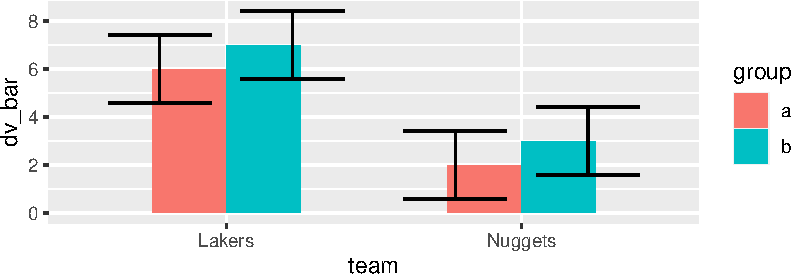
\includegraphics{r_visualization_files/figure-pdf/fig-r-basics-col-10-1.pdf}

}

\caption{\label{fig-r-basics-col-10}}

\end{figure}%

\begin{tcolorbox}[enhanced jigsaw, bottomrule=.15mm, breakable, leftrule=.75mm, left=2mm, toptitle=1mm, opacitybacktitle=0.6, bottomtitle=1mm, colframe=quarto-callout-tip-color-frame, titlerule=0mm, colback=white, colbacktitle=quarto-callout-tip-color!10!white, toprule=.15mm, opacityback=0, arc=.35mm, rightrule=.15mm, title=\textcolor{quarto-callout-tip-color}{\faLightbulb}\hspace{0.5em}{Tip}, coltitle=black]

Praktische Varianten von \texttt{geom\_errorbar()} für Streu- oder
Liniendiagramme sind \texttt{geom\_pointrange()} und
\texttt{geom\_linerange()}.

\begin{Shaded}
\begin{Highlighting}[]
\FunctionTok{ggplot}\NormalTok{(df, }\FunctionTok{aes}\NormalTok{(iv, dv)) }\SpecialCharTok{+}
  \FunctionTok{geom\_point}\NormalTok{() }\SpecialCharTok{+} 
  \FunctionTok{geom\_linerange}\NormalTok{(}\FunctionTok{aes}\NormalTok{(}\AttributeTok{ymin=}\NormalTok{dv}\DecValTok{{-}1}\NormalTok{, }\AttributeTok{ymax=}\NormalTok{dv}\SpecialCharTok{+}\DecValTok{1}\NormalTok{))}
\end{Highlighting}
\end{Shaded}

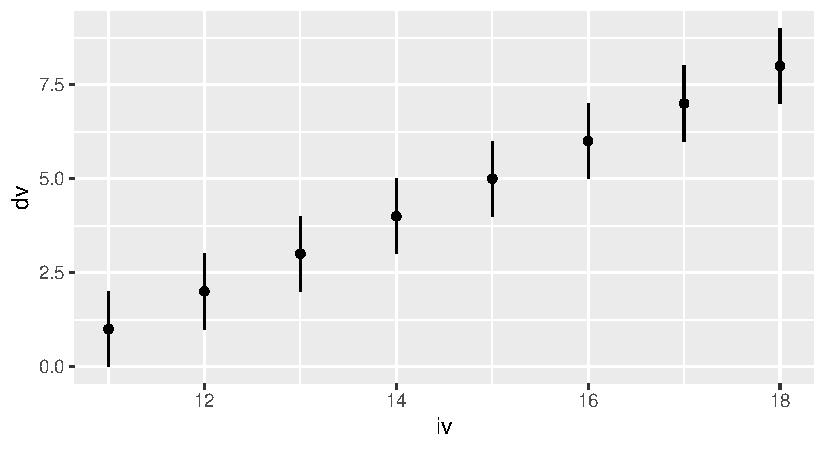
\includegraphics{r_visualization_files/figure-pdf/unnamed-chunk-35-1.pdf}

\end{tcolorbox}

\subsection{\texorpdfstring{\texttt{geom\_histogram()}}{geom\_histogram()}}\label{geom_histogram}

Schauen wir uns letztes \texttt{geom} nun noch
\texttt{geom\_histogram()} an. Mit \texttt{geom\_histogram()} können wir
ein Histogramm der Daten erstellen. Wir generieren uns dazu aber erst
noch einen neuen Datensatz, da \texttt{df} für ein Histogram etwas
unterbesetzt ist.

\begin{Shaded}
\begin{Highlighting}[]
\NormalTok{df\_hi }\OtherTok{\textless{}{-}} \FunctionTok{tibble}\NormalTok{(}\AttributeTok{x =} \FunctionTok{rnorm}\NormalTok{(}\DecValTok{100}\NormalTok{))}
\end{Highlighting}
\end{Shaded}

In \texttt{df\_hi} haben wir jetzt eine Zufallsstichprobe aus
\(N = 100\) Datenpunkte aus der \(\mathcal{N}(0,1)\) gezogen. Erstellen
wir nun mit Hilfe von \texttt{geom\_histogram()} das dazugehörende
Histogram (siehe Figure~\ref{fig-r-viz-hist-01}).

\begin{Shaded}
\begin{Highlighting}[]
\FunctionTok{ggplot}\NormalTok{(df\_hi, }\FunctionTok{aes}\NormalTok{(x)) }\SpecialCharTok{+} 
  \FunctionTok{geom\_histogram}\NormalTok{()}
\end{Highlighting}
\end{Shaded}

\begin{figure}[H]

\centering{

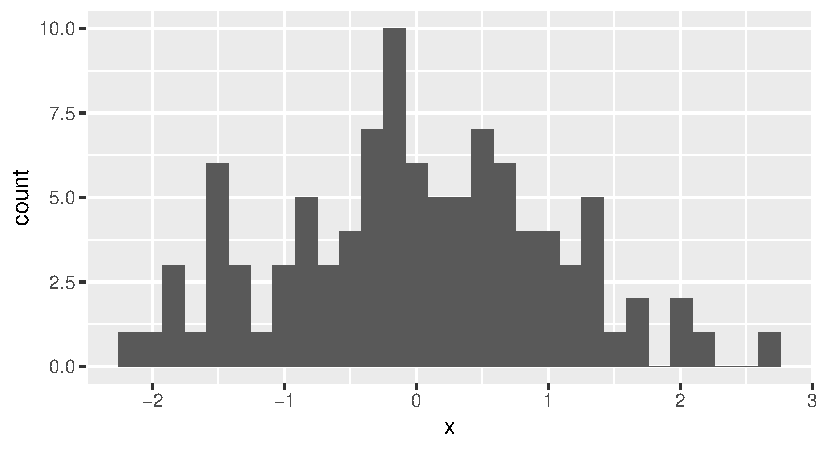
\includegraphics{r_visualization_files/figure-pdf/fig-r-viz-hist-01-1.pdf}

}

\caption{\label{fig-r-viz-hist-01}Beispiel für ein Histogram mit
\texttt{geom\_histogram()}}

\end{figure}%

\texttt{geom\_histogram()} verwendet standardmäßig \(30\) Intervalle,
daher kann mit dem Parameter \texttt{bins} die Anzahl der
Intervallunterteilungen spezifiziert werden, während mit
\texttt{binwidth} die Breite der Intervalle angegeben werden kann (siehe
Figure~\ref{fig-r-viz-hist-02}).

\begin{Shaded}
\begin{Highlighting}[]
\FunctionTok{ggplot}\NormalTok{(df\_hi, }\FunctionTok{aes}\NormalTok{(x)) }\SpecialCharTok{+} 
  \FunctionTok{geom\_histogram}\NormalTok{(}\AttributeTok{bins =} \DecValTok{20}\NormalTok{)}
\end{Highlighting}
\end{Shaded}

\begin{figure}[H]

\centering{

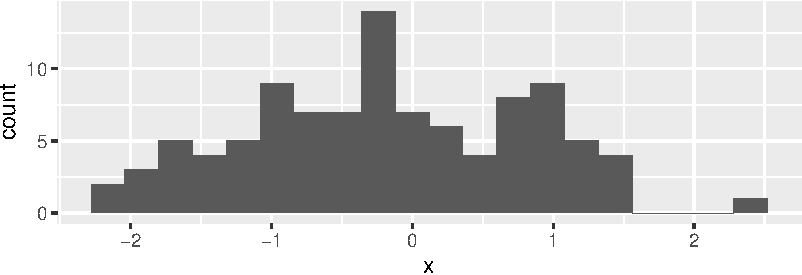
\includegraphics{r_visualization_files/figure-pdf/fig-r-viz-hist-02-1.pdf}

}

\caption{\label{fig-r-viz-hist-02}Beispiel für ein Histogram mit Angabe
der Anzahl der verwendeten Intervalle}

\end{figure}%

Standardmäßig gibt \texttt{geom\_histogram()} auf der \(y\)-Achse die
Anzahl der Datenpunkte in dem jeweiligen Intervall an. Möchten wir
lieber die relative Häufigkeit angezeigt haben, also die Anzahl der
Datenpunkte in jedem Intervall geteilt durch die Gesamtanzahl an
Punkten, dann müssen wir auf die berechneten Werte der
\texttt{geom\_histogram()} zugrundeliegenden \texttt{stat\_}-Funktion
zurückgreifen. Hinter den Kulissen sendet \texttt{geom\_histogram()} die
Daten an eine \texttt{stat\_bin()}-Funktion. \texttt{stat\_bin()}
berechnet zunächst die Intervalle, dann die Anzahl der Punkte in den
Intervallen und gibt diese wieder intern in Form eines \texttt{tibble}s
zurück. Gleichzeitig berechnet \texttt{stat\_bin()} noch die relative
Häufigkeit und schreibt diese als Variable \texttt{density} in das
\texttt{tibble}. Um auf die Variable \texttt{density} zugreifen zu
können muss eine spezielle Funktion \texttt{after\_stat()} verwendet und
in \texttt{aes()} zugewiesen werden (siehe
Figure~\ref{fig-r-viz-hist-03}).

\begin{Shaded}
\begin{Highlighting}[]
\FunctionTok{ggplot}\NormalTok{(df\_hi, }\FunctionTok{aes}\NormalTok{(x)) }\SpecialCharTok{+} 
  \FunctionTok{geom\_histogram}\NormalTok{(}\FunctionTok{aes}\NormalTok{(}\AttributeTok{y =} \FunctionTok{after\_stat}\NormalTok{(density)), }\AttributeTok{bins =} \DecValTok{20}\NormalTok{)}
\end{Highlighting}
\end{Shaded}

\begin{figure}[H]

\centering{

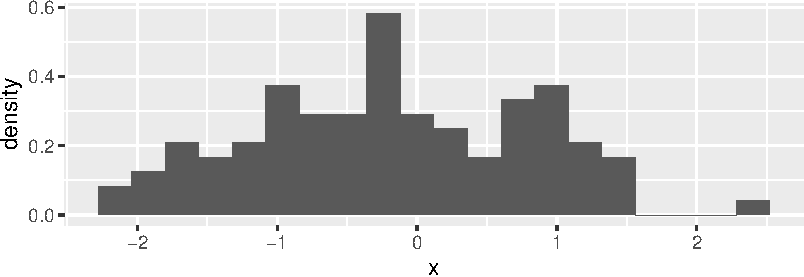
\includegraphics{r_visualization_files/figure-pdf/fig-r-viz-hist-03-1.pdf}

}

\caption{\label{fig-r-viz-hist-03}Beispiel für ein Histogram der
relativen Häufigkeiten}

\end{figure}%

\subsection{\texorpdfstring{\texttt{facet\_grid()} und
\texttt{facet\_wrap()}}{facet\_grid() und facet\_wrap()}}\label{facet_grid-und-facet_wrap}

Als nächstes kommen zwei der praktischsten Funktion in \texttt{ggplot2}
überhaupt. Mit \texttt{facet\_grid()} können wir ein Raster an Grafiken
erstellen. Hier zwei einfache Beispiel für ein horizontales und eine
vertikales Raster.

\begin{Shaded}
\begin{Highlighting}[]
\FunctionTok{ggplot}\NormalTok{(df, }\FunctionTok{aes}\NormalTok{(iv, dv)) }\SpecialCharTok{+}
  \FunctionTok{geom\_point}\NormalTok{() }\SpecialCharTok{+}
  \FunctionTok{facet\_grid}\NormalTok{(}\SpecialCharTok{\textasciitilde{}}\NormalTok{team)}
\FunctionTok{ggplot}\NormalTok{(df, }\FunctionTok{aes}\NormalTok{(iv, dv)) }\SpecialCharTok{+}
  \FunctionTok{geom\_point}\NormalTok{() }\SpecialCharTok{+}
  \FunctionTok{facet\_grid}\NormalTok{(team}\SpecialCharTok{\textasciitilde{}}\NormalTok{.)}
\end{Highlighting}
\end{Shaded}

\begin{figure}

\begin{minipage}{0.50\linewidth}

\centering{

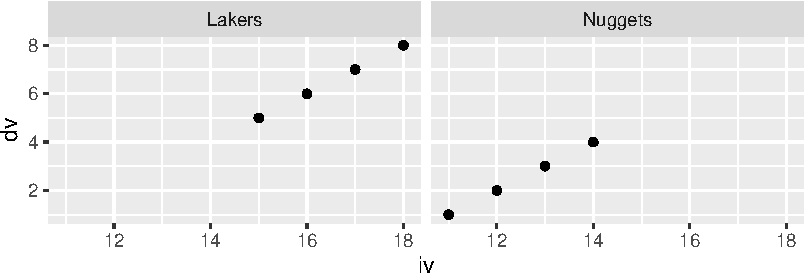
\includegraphics{r_visualization_files/figure-pdf/fig-r-basics-facet-01-1.pdf}

}

\subcaption{\label{fig-r-basics-facet-01-1}Horizontales Raster}

\end{minipage}%
%
\begin{minipage}{0.50\linewidth}

\centering{

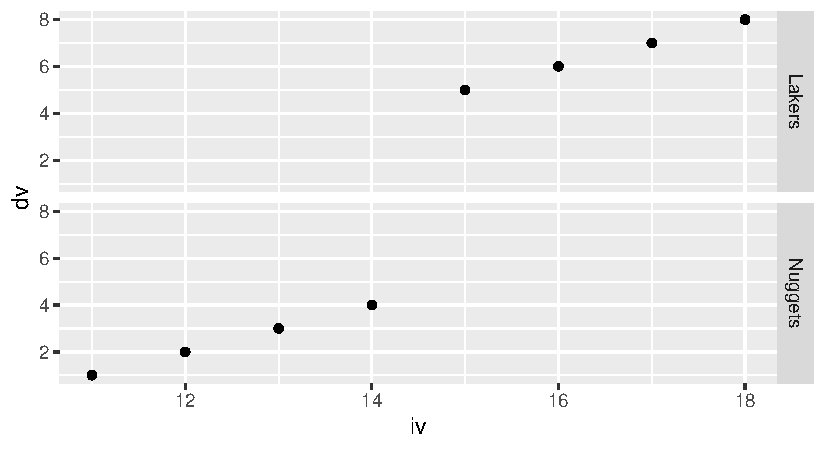
\includegraphics{r_visualization_files/figure-pdf/fig-r-basics-facet-01-2.pdf}

}

\subcaption{\label{fig-r-basics-facet-01-2}Vertikales Raster}

\end{minipage}%

\caption{\label{fig-r-basics-facet-01}Zwei einfacher Beispiel für
Grafikraster.}

\end{figure}%

Das Raster wir in \texttt{facet\_grid()} mittels einer Formel mit der
\texttt{\textasciitilde{}} spezifiziert. Nach dem Muster
\texttt{Vertikal\textasciitilde{}Horizontal}. Wenn wir ein vertikales
Raster erstellen möchten müssen wir einen Punkt \texttt{.} in die Formel
aus Syntaxgründen einfügen. Natürlich können wir auch beide gleichzeitig
verwenden. Was bei unseren Datensatz nicht wirklich spannend aussieht,
da wir zu wenig Daten dafür haben (siehe
Figure~\ref{fig-r-basics-facet-02}).

\begin{Shaded}
\begin{Highlighting}[]
\FunctionTok{ggplot}\NormalTok{(df, }\FunctionTok{aes}\NormalTok{(iv, dv)) }\SpecialCharTok{+}
  \FunctionTok{geom\_line}\NormalTok{() }\SpecialCharTok{+}
  \FunctionTok{geom\_point}\NormalTok{() }\SpecialCharTok{+}
  \FunctionTok{facet\_grid}\NormalTok{(group }\SpecialCharTok{\textasciitilde{}}\NormalTok{ team)}
\end{Highlighting}
\end{Shaded}

\begin{figure}[H]

\centering{

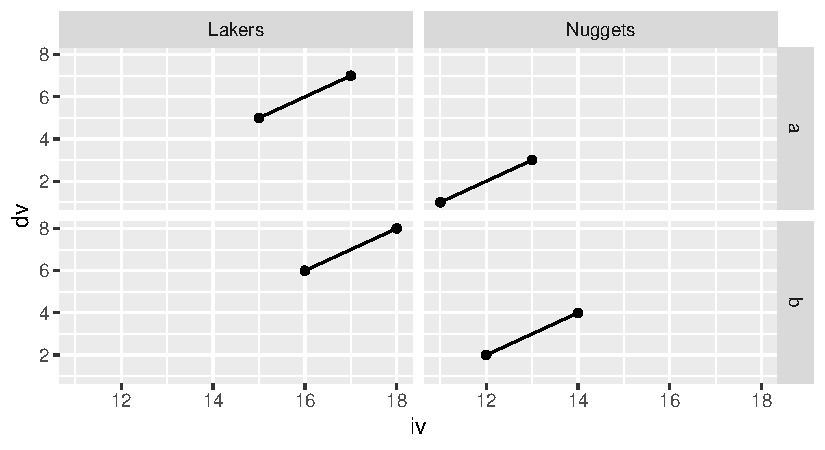
\includegraphics{r_visualization_files/figure-pdf/fig-r-basics-facet-02-1.pdf}

}

\caption{\label{fig-r-basics-facet-02}Eine vollständige Rastergrafik}

\end{figure}%

Mit \texttt{facet\_wrap()} kann ein ähnliche Effekt erreicht werden, nur
das die Untergrafiken von links oben nach rechts unten aufgebaut werden
und vor allem nützlich sind wenn wir viele Gruppen auf einmal anschauen
wollen.

\begin{Shaded}
\begin{Highlighting}[]
\NormalTok{df\_fw }\OtherTok{\textless{}{-}} \FunctionTok{tibble}\NormalTok{(}\AttributeTok{id =} \FunctionTok{paste0}\NormalTok{(}\StringTok{\textquotesingle{}P\textquotesingle{}}\NormalTok{,}\DecValTok{1}\SpecialCharTok{:}\DecValTok{10}\NormalTok{), }\AttributeTok{Wert =} \DecValTok{1}\SpecialCharTok{:}\DecValTok{10}\NormalTok{, }\AttributeTok{x =} \DecValTok{1}\NormalTok{)}
\FunctionTok{ggplot}\NormalTok{(df\_fw, }\FunctionTok{aes}\NormalTok{(x,Wert)) }\SpecialCharTok{+}
  \FunctionTok{geom\_point}\NormalTok{(}\AttributeTok{size=}\DecValTok{2}\NormalTok{) }\SpecialCharTok{+}
  \FunctionTok{facet\_wrap}\NormalTok{(}\SpecialCharTok{\textasciitilde{}}\NormalTok{id)}
\end{Highlighting}
\end{Shaded}

\begin{figure}[H]

\centering{

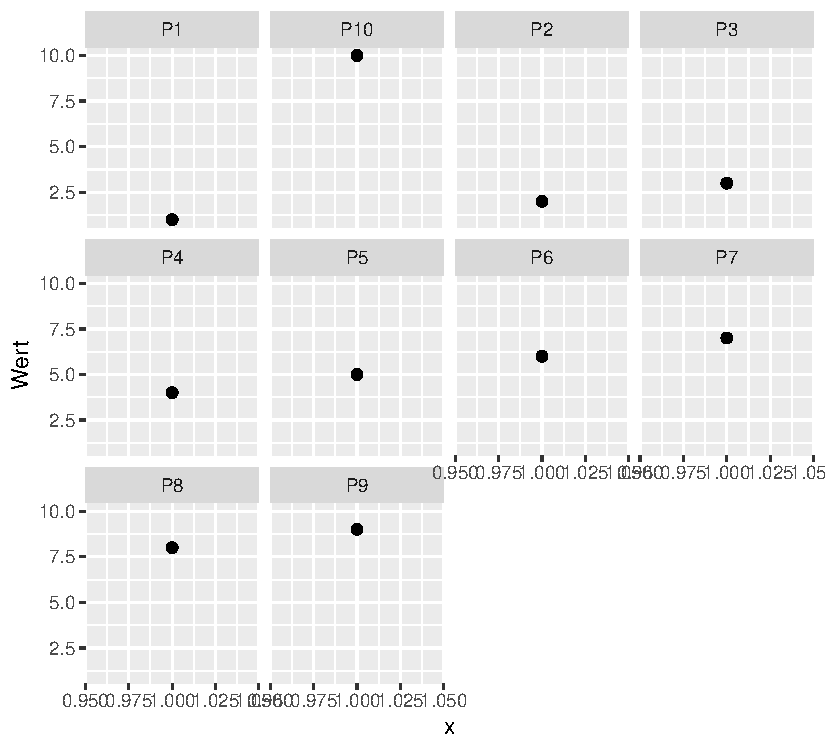
\includegraphics{r_visualization_files/figure-pdf/fig-r-basics-facet-03-1.pdf}

}

\caption{\label{fig-r-basics-facet-03}Ein Beispiel für facet\_wrap()}

\end{figure}%

\subsection{\texorpdfstring{\texttt{labs()} und
\texttt{lims()}}{labs() und lims()}}\label{labs-und-lims}

Wenn wir die Achsenbeschriftungen ändern wollen können wir dafür die
Funktion \texttt{labs()} benutzen, während \texttt{lims()} die minimalen
(maximalen) Werte der Achsen bestimmt.

\begin{Shaded}
\begin{Highlighting}[]
\FunctionTok{ggplot}\NormalTok{(df, }\FunctionTok{aes}\NormalTok{(iv, dv)) }\SpecialCharTok{+}
  \FunctionTok{geom\_point}\NormalTok{() }\SpecialCharTok{+}
  \FunctionTok{labs}\NormalTok{(}\AttributeTok{x =} \StringTok{\textquotesingle{}Die unabhängige Variable\textquotesingle{}}\NormalTok{, }\AttributeTok{y =} \StringTok{\textquotesingle{}Die abhängige Variable\textquotesingle{}}\NormalTok{) }\SpecialCharTok{+}
  \FunctionTok{lims}\NormalTok{(}\AttributeTok{x =} \FunctionTok{c}\NormalTok{(}\DecValTok{0}\NormalTok{,}\DecValTok{30}\NormalTok{), }\AttributeTok{y =} \FunctionTok{c}\NormalTok{(}\SpecialCharTok{{-}}\DecValTok{5}\NormalTok{,}\DecValTok{20}\NormalTok{))}
\end{Highlighting}
\end{Shaded}

\begin{figure}[H]

\centering{

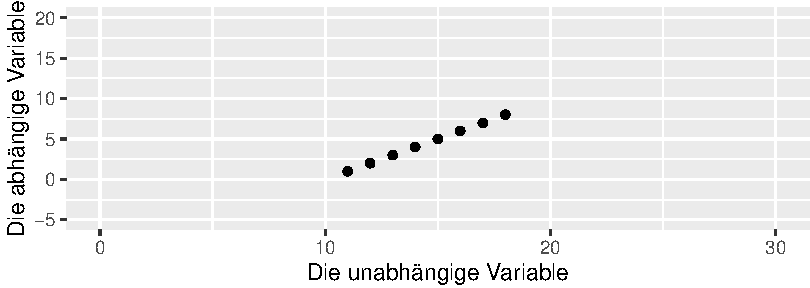
\includegraphics{r_visualization_files/figure-pdf/fig-r-basics-labs-1.pdf}

}

\caption{\label{fig-r-basics-labs}Beschriftungen und Achsenwerte mit
\texttt{labs()} und \texttt{lims()} bestimmen.}

\end{figure}%

Wenn ihr mehr Kontrolle über die Achsen benötigt gibt es die Funktionen
\texttt{scale\_x\_continuous()} für eine kontinuierliche Variable auf
der \(x\)-Achse und \texttt{scale\_x\_discrete()} für nominale Variablen
(bzw. die gleichen Funktion mit \texttt{y} anstatt \texttt{x} für die
\(y\)-Achse). Mit diesen Funktionen kann das Aussehen der Achsen
vollständig angepasst werden.

\subsection{\texorpdfstring{\texttt{theme()}}{theme()}}\label{theme}

Als letzten Punkt noch die Funktion \texttt{theme()} mit der alle
möglichen Formatierungseinstellung von \texttt{ggplot} angesprochen und
individuell angepasst werden können. Hier als einfachstes Beispiel die
Schriftgröße gleichmäßig für alle Textkomponenten in der Grafik
anpassen.

\begin{Shaded}
\begin{Highlighting}[]
\FunctionTok{ggplot}\NormalTok{(df, }\FunctionTok{aes}\NormalTok{(iv,dv)) }\SpecialCharTok{+}
  \FunctionTok{geom\_point}\NormalTok{() }\SpecialCharTok{+}
  \FunctionTok{theme}\NormalTok{(}\AttributeTok{text =} \FunctionTok{element\_text}\NormalTok{(}\AttributeTok{size =} \DecValTok{24}\NormalTok{))}
\end{Highlighting}
\end{Shaded}

\begin{figure}[H]

\centering{

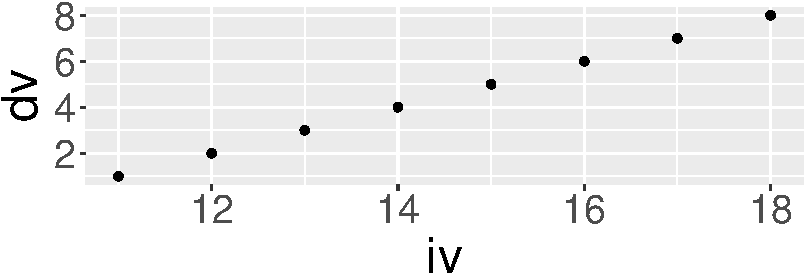
\includegraphics{r_visualization_files/figure-pdf/fig-r-basics-theme-1.pdf}

}

\caption{\label{fig-r-basics-theme}Textgrößen mit \texttt{theme()}
anpassen.}

\end{figure}%

Wenn ihr mit \texttt{theme()} arbeiten wollt/müsst, schaut euch wie
immer die umfangreiche
\href{https://ggplot2.tidyverse.org/reference/theme.html}{Dokumentation}
an.

\subsection{Weiterführendes}\label{weiterfuxfchrendes-1}

Insgesamt haben wir wieder nur die Oberfläche von \texttt{ggplot}
gekratzt. Allerdings sollte ihr mit diesen wenigen \texttt{geom}s schon
eine Großzahl eurer Anwendungsfälle abbilden können. Im Netz gibt es
eine Reihe von sehr guten freien Quellen um sich eingehender mit
\texttt{ggplot} auseinander zu setzen. Das
\href{https://r-graphics.org/}{Buch} von Chang (2018) gibt schnelle
Lösungen für konkrete Probleme. Healy (2018) gibt mehr Hilfestellungen
zur effektiven Visualisierung mit \href{https://socviz.co/}{ggplot},
während Wickham (2009) das definitive Nachschlagewerk vom
Haupprogrammier von \href{https://ggplot2-book.org/}{ggplot2} ist. Bei
Problemen ist auch wie gesagt die extrem gute
\href{https://ggplot2.tidyverse.org/}{Dokumentation} zu konsultieren.
Dazu kommen mittlerweile auch eine Reihe von Zusatzbibliotheken um
praktisch jede erdenkliche Art von Visualisierung zu erstellen. Ein
Paket das ihr auch auf jeden Fall anschauen solltes ist
\href{https://patchwork.data-imaginist.com/index.html}{\texttt{patchwork}}.

\chapter{\texorpdfstring{Literate programming in
\texttt{R}}{Literate programming in R}}\label{literate-programming-in-r}

Beim Literate programming wird Programmcode und Dokumentation
miteinander kombiniert, dabei entsteht ein Dokument das eine Mischung
Code und Dokumentation ist. Der Programmiercode wird in kleine,
verständliche Einheiten (sogenannte Chunks) unterteilt, diese Chunks
werden mit Kommentaren und Erklärungen versehen. Diese Einheiten werden
dann in einer logischen Reihenfolge angeordnet, die dem Leser den Zweck
und die Funktionsweise des Programms vermittelt. Dadurch fördert
Literate programming die Wiederverwendbarkeit, Lesbarkeit und
Wartbarkeit von Code. Im Rahmen von Datenanalysen entsteht so ein
dynamisches Dokument das alle Analyseschritte durchführt und auch
gleichzeitig diese Dokumentiert bzw. beschreibt. Dies kann direkt aus
\texttt{R} heraus generiert werden. Dies führt dazu, dass Daten, deren
Verarbeitung und die Dokumentation und Interpretation in einer Einheit
integriert sind. Letztendlich entsteht so die Möglichkeit auch direkt
fertig formatierte Publikationen aus \texttt{R} heraus zu generieren.

In \texttt{R} gibt es derzeit drei, eigentlich zweieinhalb, verschiedene
Methoden um Literatue Programming durchzuführen. Das klassische
RSweave-Format, dass auf der Integration von \texttt{R}-Code und
\emph{LaTex} beruht, das modernere RMarkdown bei dem \texttt{R}-Code und
Markdown-Syntax miteinander verbunden werden und die überarbeitete
Version von RMarkdown genannt Quarto. Bei Quarto wird wie bei RMarkdown
\texttt{R}-Code mit Markdown integriert und mittels spezieller Angaben
in einem Header in der sogenannten YAML-Syntax gesteuert. Im Rahmen des
Skripts beschäftigen wir uns nur mit Quarto.

Allgemein handelt es sich bei Quarto um ein Open-Source System für
wissenschaftliche und technische Veröffentlichungen welches Literate
Programming implementiert. Mittels Quarto können eine ganze Reihe von
unterschiedlichen Dokumenten erstellt werden von wissenschaftlichen
Zeitschriftenartikel bis zu kompletten Bücher und Webseiten. Tatsächlich
ist das vorliegende Skriptum ebenfalls mit Quarto erstellt worden.

\section{\texorpdfstring{\texttt{R}
Projekte}{R Projekte}}\label{r-projekte}

Bevor wir mit Quarto anfangen, lernen wir kurz noch \texttt{R}-Projekte
kennen, da diese eine deutliche Vereinfachung des Arbeitsprozesses mit
\texttt{R} ermöglichen.

Wenn eine Datenanalyse durchführt wird, ist es von großem Vorteil wenn
alle für die Analyse notwendigen Informationen wie Daten, Ergebnisse,
Zwischenrechnungen usw. an einem gemeinsamen Ort abgespeichert sind.
Eine einfache Lösung bietet eine dedizierter Verzeichnisordner der mit
Unterordnern so strukturiert ist, dass die Projektdateien systematisch
organisiert sind und am Besten bestimmten (möglicherweise eigenen)
Konvention folgt. So kann sicher gestellt werden, dass wenn Analysen zu
späteren Zeitpunkten wieder durchgeführt werden nahtlos an den letzten
Stand angeknüpft werden kann. In RStudio ist speziell zu diesem Zweck
ein Prozess erstellt worden der diesen Ansatz formalisiert. RStudio
bietet dazu die Möglichkeit ein \textbf{Project} zu erstellen. Unter
(File/New Project) kann dazu ein Projekt erstellt werden.

Sobald ein Projekt in RStudio erstellt wurde, d.h. ein Namen vergeben
wurde und ein Verzeichnis, das Wurzelverzeichnis, ausgewählt wurde wo
das Projekt auf dem Computer hinterlegt ist, springt \texttt{R} in
dieses Wurzelverzeichnis und macht das Verzeichnis zum
Arbeitsverzeichnis. Da das Wurzelverzeichnis nichts von
Standardverzeichnissen auf dem Computer unterscheidet können weitere
Unterverzeichniss wie zum Beispiel \emph{data}, \emph{specs},
\emph{analysis} oder was auch immer benötigt wird beliebig erstellen
werden. Das Projekt kann in RStudio geöffnet oder geschlossen werden.
Beim Öffnen springt \texttt{R} immer automatisch in das
Wurzelverzeichnis und stellt so sicher, dass alle relativen Pfade zu
Dateien korrekt aufgelöst werden können.

Eine Regel sollte im Umgang mit Projekten beachtet werden. Wann immer
auf eine Datei zugriffen wird, dann sollten relative Pfadangabe
verwendet werden. Also, anstatt
\texttt{D:/studium/master/data/studie\_01.txt}, Pfade in der Form
\texttt{/data/studie\_01.txt}. Durch die Verwendung von relativen Pfade,
können Projekte problemlos zwischen Rechnern transferieren (migriert)
werden. Die relativen Pfade stellen sicher, dass die Position von
Dateien immer in Relation zum Wurzelverzeichnis des Projekt lokalisiert
werden.

Wenn ein Projekt in RStudio neu erstellt wird, dann generiert RStudio
eine Konfigurationsdatei mit der Endung \texttt{.Rproj} in der noch
weitere Einstellungen gespeichert werden. Diese können über die
Projekteinstellungen über den Menupunkt (Tools/Project Options)
anpassen.

\section{Quarto-Dokumente}\label{quarto-dokumente}

\subsection{Markdown}\label{markdown}

Bei Quarto-Dokumenten handelt es sich um Dateien mit der Endung
\texttt{.qmd}, die gleichzeitig Text wie auch \texttt{R}-Code enthalten
können. Die Textsegmente sind dabei nicht nur einfache Kommentare
(\texttt{\#}) im Code, sondern vollständig formatierte Textsegmente, wie
wir sie aus Word und ähnlichen Programmen kennen. Die Formatierung der
Textkomponenten erfolgt mit der sogenannten Markdown-Syntax. Markdown
ist eine einfache Auszeichnungssprache die es erlaubt
Formatierungsanweisungen in den Text zu integrieren.

Soll zum Beispiel eine Wort fett gedruckt werden, dann wird das Wort mit
zwei \texttt{**} eingeschlossen. In
Table~\ref{tbl-markdown-text-formatting} sind ein paar Beispiel
angezeigt.

\begin{longtable}[]{@{}
  >{\raggedright\arraybackslash}p{(\columnwidth - 2\tabcolsep) * \real{0.3333}}
  >{\raggedright\arraybackslash}p{(\columnwidth - 2\tabcolsep) * \real{0.3194}}@{}}
\caption{Beispiele für Textformatierung mit
Markdown}\label{tbl-markdown-text-formatting}\tabularnewline
\toprule\noalign{}
\begin{minipage}[b]{\linewidth}\raggedright
Markdown Syntax
\end{minipage} & \begin{minipage}[b]{\linewidth}\raggedright
Formatierung
\end{minipage} \\
\midrule\noalign{}
\endfirsthead
\toprule\noalign{}
\begin{minipage}[b]{\linewidth}\raggedright
Markdown Syntax
\end{minipage} & \begin{minipage}[b]{\linewidth}\raggedright
Formatierung
\end{minipage} \\
\midrule\noalign{}
\endhead
\bottomrule\noalign{}
\endlastfoot
`\emph{kursiv}, \textbf{fett}, & \emph{kursiv}, \textbf{fett}, \\
\texttt{hoch\^{}2\^{}\ ,\ tief\textasciitilde{}2\textasciitilde{}} &
hoch\textsuperscript{2} , tief\textsubscript{2} \\
\texttt{\textasciitilde{}\textasciitilde{}durchgestrichen\textasciitilde{}\textasciitilde{}}
& \st{durchgestrichen} \\
\end{longtable}

D.h. mittels Markdown wird die Formatierung von Text mit relativ einfach
Sonderzeichen durchgeführt. So können beispielsweise Listen mittels der
folgenden Formatierung definiert werden (siehe
Table~\ref{tbl-markdown-lists}).

\begin{longtable}[]{@{}
  >{\raggedright\arraybackslash}p{(\columnwidth - 2\tabcolsep) * \real{0.5000}}
  >{\raggedright\arraybackslash}p{(\columnwidth - 2\tabcolsep) * \real{0.5000}}@{}}
\caption{Beispiele für Listenformatierungen mit
Markdown}\label{tbl-markdown-lists}\tabularnewline
\toprule\noalign{}
\begin{minipage}[b]{\linewidth}\raggedright
Markdown Syntax
\end{minipage} & \begin{minipage}[b]{\linewidth}\raggedright
Formatierung
\end{minipage} \\
\midrule\noalign{}
\endfirsthead
\toprule\noalign{}
\begin{minipage}[b]{\linewidth}\raggedright
Markdown Syntax
\end{minipage} & \begin{minipage}[b]{\linewidth}\raggedright
Formatierung
\end{minipage} \\
\midrule\noalign{}
\endhead
\bottomrule\noalign{}
\endlastfoot
\begin{minipage}[t]{\linewidth}\raggedright
* ungeordnete Liste\\
\strut ~~~~+ Unterelement 1\\
\strut ~~~~+ Unterelement 2\\
\strut ~~~~~~~~- Unterunterelement 1
\end{minipage} & \begin{minipage}[t]{\linewidth}\raggedright
\begin{itemize}
\tightlist
\item
  ungeordnete Liste

  \begin{itemize}
  \tightlist
  \item
    Unterelement 1
  \item
    Unterelement 2

    \begin{itemize}
    \tightlist
    \item
      Unterunterelement 1
    \end{itemize}
  \end{itemize}
\end{itemize}
\end{minipage} \\
\begin{minipage}[t]{\linewidth}\raggedright
1. geordnete Liste\\
2. Element 2\\
\strut ~~~i) Unterelement 1\\
\strut ~~~~~~A. Unterunterelement 1
\end{minipage} & \begin{minipage}[t]{\linewidth}\raggedright
\begin{enumerate}
\def\labelenumi{\arabic{enumi}.}
\tightlist
\item
  geordnete Liste
\item
  Element 2

  \begin{enumerate}
  \def\labelenumii{\roman{enumii})}
  \tightlist
  \item
    Unterelement 1

    \begin{enumerate}
    \def\labelenumiii{\Alph{enumiii}.}
    \tightlist
    \item
      Unterunterelement 1
    \end{enumerate}
  \end{enumerate}
\end{enumerate}
\end{minipage} \\
\end{longtable}

Markdown im Zusammenspiel mit Quarto bietet alle nur erdenklichen
Formatierungsmöglichkeiten und Feinheiten um die gewünschten
Formatierungen einzustellen. Da die verschiedenen Begriffe den Umfang
des Skripts deutlich sprengen würden wird hier darauf verzichtet den
gesamten Umfang von Quarto und Markdown zu beschreiben. Da Quarto zudem
ein noch relativ neues Projekt ist kommen immer wieder neue Features
dazu. Daher sollte die sehr gute Dokumentation von
\href{https://quarto.org/docs/guide/}{Quarto} immer die erste Adresse
für alle Fragen sein. Der große Vorteil von Quarto + Markdown besteht
letztendlich darin, dass alle Dokumente nichts weiteres als Textdateien
sind und letztendlich nicht einmal nur mit RStudio bearbeitet werden
müssen sondern mittels jedes beliebigen Texteditor erstellt und
verändert werden können.

\subsection{\texorpdfstring{\texttt{R}-Code in
Quarto-Dokumenten}{R-Code in Quarto-Dokumenten}}\label{r-code-in-quarto-dokumenten}

D \texttt{R}-Code in Quarto-Dokumente integriert ist, schaun wir uns
noch kurz die Erstellen von Chunks (auch Code blocks genannt) an.

Von \texttt{R} auszuführende Codeblöcke werden ebenfalls mittels
spezieller Formatierungszeichen ausgezeichnet. Der Anfang eines
Codeblocks wird mit drei backticks (SHIFT+´) gefolgt von \texttt{\{r\}}
eingeleitet. Das Endes des Codeblock wird mittels dreier backticks
abgeschlossen.
\texttt{\textasciigrave{}\textasciigrave{}\textasciigrave{}\{r\}\ R\ Code}).
Diese Codeblöcke werden während des rendern, also des Formatierens des
Quarto-Dokuments, intern durch \texttt{R} ausgeführt.

\begin{tcolorbox}[enhanced jigsaw, bottomrule=.15mm, breakable, leftrule=.75mm, left=2mm, toptitle=1mm, opacitybacktitle=0.6, bottomtitle=1mm, colframe=quarto-callout-tip-color-frame, titlerule=0mm, colback=white, colbacktitle=quarto-callout-tip-color!10!white, toprule=.15mm, opacityback=0, arc=.35mm, rightrule=.15mm, title=\textcolor{quarto-callout-tip-color}{\faLightbulb}\hspace{0.5em}{Tip}, coltitle=black]

In R-Studio ist der short-cut \texttt{STRG+SHIFT+i} (windows) definiert
um einen Codeblock an der aktuellen Cursorposition einzufügen.

\end{tcolorbox}

Ein Beispiel für einen einfachen Codeblock sieht dann wie folgt aus:

\begin{Shaded}
\begin{Highlighting}[]
\InformationTok{\textasciigrave{}\textasciigrave{}\textasciigrave{}\{r\}}
\InformationTok{a \textless{}{-} 3}
\InformationTok{b \textless{}{-} 4}
\InformationTok{a + b}
\InformationTok{\textasciigrave{}\textasciigrave{}\textasciigrave{}}
\end{Highlighting}
\end{Shaded}

Die Variablen die in den jeweiligen Codeblöcken definiert werden stehen
in weiteren, nachfolgenden Codeblöcken in dem Quartodokument zur
Verfügung.

Einzelne Codeblöcke können in R-Studio getrennt ausgeführt werden. Dazu
muss der Cursor in dem Block sein und entweder mit PLAY-Button
oben-recht im Block oder mit dem short-cut
\texttt{STRG+SHIFT+ENTER} (windows). Um das ganze Dokument zu rendern
kann entweder der Render-Button oberhalb des Dokuments verwendet werden
oder wiederum der short-cut \texttt{STRG+SHIFT+k} (windows).

Wenn wir unseres vorhergehendes Workflow-Beispiel nehmen, dann könnte
ein gekürztes Quarto-Dokument wie folgt aussehen:

\begin{Shaded}
\begin{Highlighting}[]
\CommentTok{{-}{-}{-}}
\AnnotationTok{title:}\CommentTok{ "Analyse des Körperfettgehalts in zwei Gruppen"}
\AnnotationTok{author:}\CommentTok{ "Martina Muster"}
\CommentTok{{-}{-}{-}}
\FunctionTok{\# Einleitung}

\NormalTok{Nach Schmidt et al. (2023) ist davon auszugehen, dass eine Manipulation von XYZ}
\NormalTok{dazu führt, dass ... . Diese Hypothese soll anhand einer neuen Stichprobe}
\NormalTok{überprüft werden.}

\FunctionTok{\# Methodik}

\NormalTok{...}

\FunctionTok{\# Analyse}

\FunctionTok{\#\# Bibliotheken}

\NormalTok{Für die Bearbeitung der Daten, werden die folgenden Bibliotheken benötigt.}
\InformationTok{\textasciigrave{}\textasciigrave{}\textasciigrave{}\{r\}}
\InformationTok{library(readr)}
\InformationTok{library(ggplot2)}
\InformationTok{library(dplyr)}
\InformationTok{\textasciigrave{}\textasciigrave{}\textasciigrave{}}

\FunctionTok{\#\# Daten einlesen}

\NormalTok{Die Rohdaten befinden sich in der Textdatei "bfp\_data.txt".}
\NormalTok{**Achtung**, darauf achten, dass der Dateipfad korrekt ist.}

\InformationTok{\textasciigrave{}\textasciigrave{}\textasciigrave{}\{r\}}
\InformationTok{bfp \textless{}{-} read\_csv(file = \textquotesingle{}bfp\_data.txt\textquotesingle{})}
\InformationTok{\textasciigrave{}\textasciigrave{}\textasciigrave{}}

\FunctionTok{\#\# Daten bearbeiten}
\NormalTok{Ein Datenpunkt ist \textasciitilde{}fehlerhaft\textasciitilde{}, und zeigt einen Wert von $BFP \textgreater{} 100$, was}
\NormalTok{nicht physiologisch plausibel. Daher wird dieser Wert ausgeschlossen.}

\InformationTok{\textasciigrave{}\textasciigrave{}\textasciigrave{}\{r\}}
\InformationTok{bfp\_clean \textless{}{-} filter(bfp, BFP \textless{}= 100)}
\InformationTok{\textasciigrave{}\textasciigrave{}\textasciigrave{}}

\NormalTok{Die Daten zur Analyse befinden sich jetzt in der Variablen }\InformationTok{\textasciigrave{}bfp\_clean\textasciigrave{}}\NormalTok{.}

\FunctionTok{\# Diskussion}

\NormalTok{...}

\FunctionTok{\# Zusammenfassung}

\NormalTok{...}
\end{Highlighting}
\end{Shaded}

Zu Beginn des Quarto-Dokuments findet sich ein Abschnitt der mit
\texttt{-\/-\/-} abgegrenzt ist. Dies ist der sogenannte YAML-Header.
YAML ist ebenfalls eine einfache Auszeichnungssprache (\textbf{yet}
\textbf{a}nother \textbf{m}arkup \textbf{l}anguage). Im Header werden
verschiedene Formatierungseinstellung für das Quarto-Dokument definiert.
Hier können zum Beispiel auch weitere Dokumente wie
Zitationsbibliotheken und Zitationsstyle eingebunden werden, da Quarto
die Integration von Referenzen und Zitationen innerhalb der Dokumente
vollständig unterstützt. Wie bereits erwähnt ist das Quarto-System sehr
umfangreich und kann hier leider nicht weiter besprochen werden.

\part{Statistik - Die Grundlagen}

Die erste Frage die sich bei der Anwendung von statistischen Verfahren
stellt ist: Wofür benötigen wir Statistik überhaupt?

Beginnen wir mit einem einfachen Beispiel. Es wurde ein Datensatz
gesammelt, bei dem zwei Gruppen miteinander verglichen wurden. Die eine
Gruppe bezeichnen wir als Treatmentgruppe (TRT) und hat beispielsweise
eine spezielle Krafttraining durchgeführt, während wir die andere Gruppe
als Kontrollgruppe (CON) bezeichnen die ein \emph{übliches}
Krafttraining durchgeführt hat. Beide Gruppen sind gleich groß gewesen
und bestehen jeweils aus \(N = 20\) Personen. Die Teilnehmerinnen und
Teilnehmer sind auch zufällig in die beiden Gruppen eingeteilt worden,
so dass keine Unterschied zwischen den beiden Gruppen vor Beginn des
Trainings bestand. Es wurde nach der Trainingsperiode das folgende
Ergebnis erhalten (siehe Figure~\ref{fig-why_stats}).

\begin{figure}

\centering{

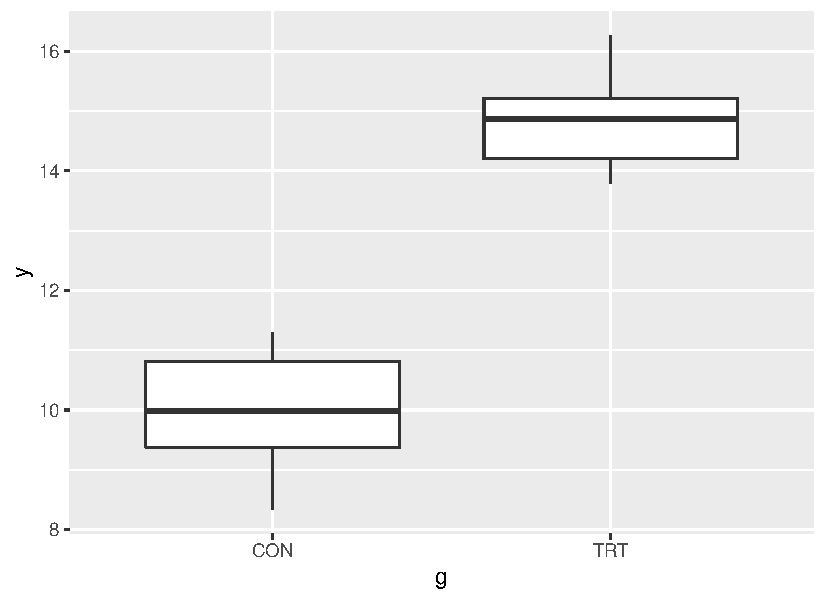
\includegraphics{stats_title_files/figure-pdf/fig-why_stats-1.pdf}

}

\caption{\label{fig-why\_stats}Boxplot der Kontroll- und der
Treatmentgruppe bezüglich einer abhängigen Variable (Rohdaten als rote
Punkte)}

\end{figure}%

In Figure~\ref{fig-why_stats} sind die Daten mittels eines Boxplots
zusammen mit den Rohdaten als rote Punkte dargestellt. Die abhängige
Variable ist die Verbesserung in der Kraftfähigkeit in \(N\). Die Daten
zeigen eigentlich relativ deutlich, dass die Verbesserung in der
Treatmentgruppe deutlich höher ausgefallen ist, als diejenige in der
Kontrollgruppe. Eine Darstellung in Form einer Tabelle kommt
erwartungsgemäß zu keiner anderen Interpretation der Daten (siehe
Table~\ref{tbl-stats-why}).

\begin{longtable}[]{@{}lrr@{}}

\caption{\label{tbl-stats-why}Mittelwert und Standardabweichung der
Kraftdaten.}

\tabularnewline

\toprule\noalign{}
Gruppe & \(\bar{F}\) & SD \\
\midrule\noalign{}
\endhead
\bottomrule\noalign{}
\endlastfoot
CON & 10.05 & 0.89 \\
TRT & 14.83 & 0.78 \\

\end{longtable}

Der Mittelwert in der Treatmentgruppe ist deutlich höher als derjenige
in der Kontrollgruppe. Vor allem unter Berücksichtigung der
Standardabweichung, welche ein Maß für die Streuung der Daten ist, sind
die Unterschied zwischen den beiden Gruppen wohl bedeutsam.

Warum ist es nicht ausreichend das Offensichtliche zu dokumentieren?
Warum ist eine statistische Analyse der Daten überhaupt notwendig?

Die Antwort auf diese Fragen werden wir in den folgenden Abschnitt
erarbeiten. Im Zuge dessen werden wir die notwendigen Werkzeuge
entwickeln um die verschiedenen, einer statistischen Analyse von Daten
zugrundeliegenden, Schritte zu verstehen und anwenden zu können. Dabei
lässt sich leider die Mathematik und die damit verbundene Abstraktion
nicht vollständig umgehen wird aber auf ein Mindestmaß gehalten.

\chapter{Eine kleine Welt der
Unsicherheit}\label{eine-kleine-welt-der-unsicherheit}

Beginnen wir mit eine einfachen Modell. Dazu nehmen beginnen mit einer
übersichtlichen kleinen Welt. Die Welt über die wir eine Aussage treffen
wollen besteht daher nur aus insgesamt 20 Personen. In
Figure~\ref{fig-small-world} sind Bewohner unserer Welt einzeln zu
sehen. Die Gesamtheit aller Personen (allgemein Objekte) über die wir
eine Aussage treffen wollen bezeichnen wir als die
Population\index{Population}.

\begin{figure}

\centering{

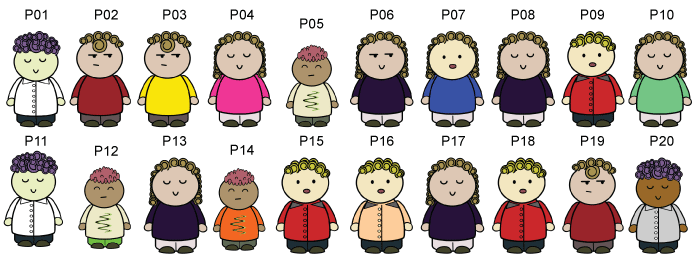
\includegraphics{pics/small_world.png}

}

\caption{\label{fig-small-world}Eine kleine Welt}

\end{figure}%

\begin{definition}[Population]\protect\hypertarget{def-population}{}\label{def-population}

Die Gesamtheit aller Objekte/Dinge/Personen über die eine Aussage
getroffen werden soll wird als Population oder Grundgesamtheit
bezeichnet.

\end{definition}

\section{Ein Experiment}\label{ein-experiment}

Wir wollen nun ein Experiment, eine Krafttrainingsstudie, durchführen um
zu überprüfen ob das Training die Beinkraft erhöht. Wir haben allerdings
nur sehr wenige Ressourcen zur Verfügung (bzw. wir sind faul) und können
daher nur insgesamt sechs Messungen durchführen. Aus einem kürzlich
durchgeführten Census haben wir aber die Beinkraftwerte der ganzen
Population. Stellen wir die Kraftwerte zunächst mittels einer Tabelle
dar (siehe Table~\ref{tbl-sts-basics-world})

\begin{longtable}[]{@{}lr@{}}

\caption{\label{tbl-sts-basics-world}Kraftwerte (in Newton) der
Lummerländer an der einbeinigen Beinpresse}

\tabularnewline

\toprule\noalign{}
ID & Kraft{[}N{]} \\
\midrule\noalign{}
\endhead
\bottomrule\noalign{}
\endlastfoot
P01 & 2414 \\
P02 & 2462 \\
P03 & 2178 \\
P04 & 2013 \\
P05 & 2194 \\
P06 & 2425 \\
P07 & 2305 \\
P08 & 2117 \\
P09 & 2298 \\
P10 & 2228 \\
P11 & 2243 \\
P12 & 2497 \\
P13 & 1800 \\
P14 & 2152 \\
P15 & 2089 \\
P16 & 2090 \\
P17 & 3200 \\
P18 & 2196 \\
P19 & 2485 \\
P20 & 2440 \\

\end{longtable}

Selbst bei 20 Werten ist diese Darstellung mittels einer Tabelle leider
wenig übersichtlich. Wir müssen Zeile für Zeile die Tabelle durchgehen
und uns spezifische Kennwerte notieren. Beispielsweise könnten wir
notieren, dass der Maximalwert der Beinkraft bei \(3200\)N für P17 und
der Minimalwert von P13 bei \(1800\)N liegt. Aber wirklich übersichtlich
ist die Darstellung in Form einer Tabelle nicht. Für solche univariaten
Daten (uni = eins) kann eine übersichtlichere Darstellung mittels eines
sogenannten Dotplots erreicht werden (siehe
Figure~\ref{fig-sts-basics-lummer-dotplot}).

\begin{figure}

\centering{

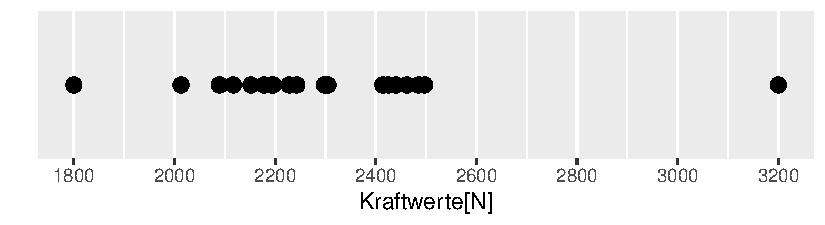
\includegraphics{stats_basics_files/figure-pdf/fig-sts-basics-lummer-dotplot-1.pdf}

}

\caption{\label{fig-sts-basics-lummer-dotplot}Dotplot der
Lummerlandkraftdaten}

\end{figure}%

Hier kann deutlich schneller abgelesen werden welchen Wert das Minimum
bzw. das Maximum annimmt. Die graphische Darstellung erlaubt weiterhin
direkt abzuschätzen in welchem Bereich sich der Großteil der Daten
befindet. Allerdings wird durch diese Art der Darstellung die
Information über welche Person die jeweiligen Werte besitzt nicht mehr
dargestellt. Dies stellt allerdings nicht zwingend ein Problem dar, da
wir in den meisten Fällen soweiso aussagen über die Gruppe und weniger
über einzelne Personen machen wollen. Ein Dotplot hat auch gleichzeitig
den Vorteil, dass wir die Verteilung der Werte abschätzen können. In
welchem Bereich liegen die meisten Datenwerte? Liegen die Werte eng
beineinander oder streuen die Werte sehr stark? Gibt es einzelne Werte
die sehr unterschiedlich sind von den anderen Werten? Dies sind alles
Fragen die notwendig sind um einen Datensatz und dessen Eigenschaften
beurteilen zu können.

Gehen wir jetzt von der folgenden Fragestellung aus. Wir wollen den
Gesundheitsstatus unserer Lummerländer verbessern und wollen dazu ein
Krafttraining für die Beine durchführen. Da wir evidenzbasiert arbeiten
wollen, möchten wir überprüfen ob das Training wirklich ein Verbesserung
der Beinkraft durch das Training stattfindet. Um die Experiment zu
vereinfachen, und da es sich mehr um eine Gedankenexperiment handelt,
gehen wir von einem perfekten Krafttraining aus. D.h wir führen eine
perfekte Intervention durch.

Das Beinkrafttraining sei also perfekt und verbessert die Kraftleistung
um genau \(+100\)N. Dieser Kraftzuwachs ist unabhängig davon welche
Person aus unserer Population das Training durchführt (Ist das eine
realistische Annahme?). Um die Effektivität des Training abzuschätzen
vergleichen wir zwei Gruppen miteinander. Eine Interventionsgruppe und
eine Kontrollgruppe. In beiden Gruppen sollen jeweils
\(n_{\text{TRT}} = n_{\text{CON}} = 3\) TeilnehmerInnen bzw. Teilnehmer
einbezogen werden da wir nicht mehr Ressourcen für mehr ProbandInnen
haben.

Um die spätere Diskussion zu vereinfachen, führen wir etwas Terminologie
ein.

\begin{definition}[Abhängige Variablen
\index{abhängige Variable}]\protect\hypertarget{def-dep-var}{}\label{def-dep-var}

Die abhängige Variable ist diejenige Variable, die in einer Studie
beobachtet, gemessen oder analysiert wird. Die abhängige Variable wird
oft als ``Effekt'' betrachtet.

\end{definition}

\begin{definition}[Unabhängige Variable
\index{unabhängige Variable}]\protect\hypertarget{def-indep-var}{}\label{def-indep-var}

Die unabhängige Variable ist die Variable, die in einer Studie oder
einem Experiment manipuliert oder kontrolliert wird. Die unabhängige
Variable wird oft als ``Ursache'' betrachtet, da sie den potenziellen
Einfluss auf die abhängige Variable repräsentiert.

\end{definition}

In unserem Experiment ist die Gruppenzugehörigkeit die unabhängige
Variable und die Beinkraft die abhängige Variable. Wir untersuchen den
Effekt der Gruppenzugehörigkeit auf die Beinkraft. Die Gruppe ist die
Ursache für mögliche Effekte auf die Beinkraft.

Wir gehen jetzt davon aus, dass wir die Daten aus dem Census nicht
vorliegen haben. Dies kommt einer tatsächlichen Durchführung des
Experiment näher, wo wir auch nicht wissen würden welche Beinkraft die
TeilnehmerInnen vor dem Experiment hätten. Die erste Frage die sich nun
stellt ist wie wir die sechs Personen aus unserer Population auswählen
und wie teilen wir die sechs Personen in die beiden Gruppen auf?

Wir könnten zum Beispiel die ersten drei Personen in die
Interventionsgruppe und die letzten drei in die Kontrollgruppe stecken.
Allerdings wenn wenn die Personen in irgendeiner Form sortiert sind,
z.B. allgemeiner Gesundheitsstatus, Arbeitstätigkeit usw. dann würde
diese Sortierung in den Gruppen auftreten. D.h. wir hätten sogenannte
Störvariablen \index{Störvariable} die unser Ergebnis verfälschen
würden.

\begin{definition}[Störvariable]\protect\hypertarget{def-confounder}{}\label{def-confounder}

Eine Störvariable ist eine Variable die einen Einfluss auf die
unabhängige Variable hat, deren Einfluss jedoch nicht kontrolliert wurde
bzw. die Variable ist nicht Hauptinteresse der Untersuchung.

\end{definition}

Im Zweifelsfall kann davon ausgegangen werden, dass es immer eine ganze
Reiche von Störvariablen gibt, von denen ich zum Teil gar nichts weiß,
dass sie bestehen. Nach etwas überlegen kommen wir darauf, dass wir am
besten eine zufällige Stichprobe ziehen sollten (Warum?). Für führen
eine sogenannte Randomisierung durch.

\begin{definition}[Randomisierung
\index{Randomisierung}]\protect\hypertarget{def-randomisierung}{}\label{def-randomisierung}

Mit Randomisierung wird der Prozess der zufälligen Zuweisung von
Probanden oder Elementen zu verschiedenen Gruppen oder Bedingungen in
einem Experiment bezeichnet. Die Randomisierung wird verwendet, um
sicherzustellen, dass die Auswahl und Zuordnung der Elemente frei von
systematischer Beeinflussung erfolgt.

\end{definition}

\begin{definition}[Stichprobe]\protect\hypertarget{def-sample}{}\label{def-sample}

Eine Stichprobe\index{Stichprobe} ist eine Teilmenge der Objekte aus der
Population.

\end{definition}

\begin{definition}[Zufallsstichprobe]\protect\hypertarget{def-random-sample}{}\label{def-random-sample}

Eine Zufallsstichprobe\index{Zufallsstichprobe} ist eine Teilmenge der
Objekte aus der Population die \emph{zufällig} ausgewählt wurde.

\end{definition}

Die sechs Personen unserer Stichprobe werden dann zufällig auf die
beiden Gruppen aufgeteilt. (Warum zufällig?)

Mit einem Zufallszahlengeneratoren haben wir die Zahlen
\(i = \{3,7,8,9,10,20\}\) gezogen. Die entsprechenden Personen werden
aus der Population anhand der ID ausgewählt. Anschließend teil wieder
ein Zufallszahlengenerator die sechs Personen in die beiden Gruppen ein
(siehe Figure~\ref{fig-stats-basics-sample-01}).

\begin{figure}

\centering{

\includegraphics[width=3.61in,height=4.97in]{stats_basics_files/figure-latex/mermaid-figure-1.png}

}

\caption{\label{fig-stats-basics-sample-01}Ablaufdiagramm der
Gruppenzuweisung.}

\end{figure}%

In Table~\ref{tbl-sts-basics-experiment-1} ist die Stichprobe und
Zuteilung in die Gruppen zu sehen.

\begin{longtable}[]{@{}lrl@{}}

\caption{\label{tbl-sts-basics-experiment-1}Zufällig ausgewählte
Stichprobe mit \(N=6\) und die Zuteilung in Kontroll- (CON) und
Interventionsgruppe (TRT).}

\tabularnewline

\toprule\noalign{}
ID & Kraft{[}N{]} & Gruppe \\
\midrule\noalign{}
\endhead
\bottomrule\noalign{}
\endlastfoot
P08 & 2117 & CON \\
P09 & 2298 & CON \\
P03 & 2178 & CON \\
P07 & 2305 & TRT \\
P10 & 2228 & TRT \\
P20 & 2440 & TRT \\

\end{longtable}

Mit diesen sechs Personen führen wir jetzt unser Experiment durch. Die
drei Personen aus der Kontrollgruppe, unterlaufen im
Interventionszeitraum nur ein Stretchtraining während die
Interventionsgruppe zweimal die Woche für 12 Wochen unser perfektes
Krafttraining durchführt. Nach diesem Zeitraum messen wir alle Personen
aus beiden Gruppen und erhalten das folgende Ergebnis (siehe
Table~\ref{tbl-sts-basics-sample-1}). Nochmal zur Erinnerung, wir nehmen
an, dass wir das Ergebnis aus dem Census nicht kennen.

\begin{table}

\caption{\label{tbl-sts-basics-sample-1}Ergebnis der Intervention in
Experiment 1 für die Kontroll- und die Interventionsgruppe.}

\begin{minipage}{0.50\linewidth}

\subcaption{\label{tbl-sts-basics-sample-1-1}Kontrollgruppe}

\centering{

\begin{tabular}{lr}
\toprule
ID & Kraft{[}N{]}\\
\midrule
P08 & 2117\\
P09 & 2298\\
P03 & 2178\\
\(\bar{K}\) & 2198\\
\bottomrule
\end{tabular}

}

\end{minipage}%
%
\begin{minipage}{0.50\linewidth}

\subcaption{\label{tbl-sts-basics-sample-1-2}Interventionsgruppe}

\centering{

\begin{tabular}{lr}
\toprule
ID & Kraft{[}N{]}\\
\midrule
P07 & 2405\\
P10 & 2328\\
P20 & 2540\\
\(\bar{K}\) & 2424\\
\bottomrule
\end{tabular}

}

\end{minipage}%

\end{table}%

Letztendlich haben wir in der Interventionsgruppe nur die Ausgangswerte
aus dem Census genommen und \(100\)N dazuaddiert. Für beide Gruppen ist
in Table~\ref{tbl-sts-basics-sample-1} jeweils noch der
Mittelwert\index{Mittelwert} angezeigt, um die Gruppen leichter
miteinander vergleichen zu können. Später werden wir noch weitere Maße
kennenlernen die es ermöglichen zwei Mengen von Werten miteinander zu
vergleichen. Der Mittelwert ist dabei derjenige der wenn schon aus der
Schule kennen.

\begin{definition}[Mittelwert]\protect\hypertarget{def-Mittelwert}{}\label{def-Mittelwert}

Der Mittelwert \(\bar{x}\) über \(n\) Werte berechnet sich nach der
Formel:

\begin{equation}\phantomsection\label{eq-mean}{
\bar{x} = \frac{\sum_{i=1}^n x_i}{n}
}\end{equation}

Der Mittelwert wird mit einem Strich über der Variable dargestellt.

\end{definition}

Damit haben wir auch schon direkt ein neues Konzept aus der Statistik
kennengelernt. Nämlich das der Statistik\index{Statistik}. Ein Wert der
mittels der Werte aus der Stichprobe berechnet wird, wird als Statistik
bezeichnet.

\begin{definition}[Statistik]\protect\hypertarget{def-Statistik}{}\label{def-Statistik}

Ein auf einer Stichprobe berechnet Wert, wird als Statistik bezeichnet.

\end{definition}

Um jetzt Unterschied zwischen den beiden Gruppen zu untersuchen
berechnen wir die Differenz D zwischen den beiden Mittelwerten
\(D = \bar{K}_{\text{TRT}} - \bar{K}_{\text{CON}}\). Die Differenz kann
natürlich auch in die andere Richtung berechnet werden und es würde sich
das Vorzeichen ändern. Hier gibt es keine Vorgaben, sondern die Richtung
kann frei bestimmt werden. Wenn bekannt ist in welcher Richtung der
Unterschied berechnet wird, dann stellt dies keine Problem dar. Im
vorliegenden Fall ziehen wir die Interventionsgruppe von der
Kontrollgruppe ab, da wir davon ausgehen, dass die Intervention zu einer
Krafterhöhung führt und wir dadurch einen positiven Unterschied erhalten
(vgl. Equation~\ref{eq-sts-basics-ex1-d})

\begin{equation}\phantomsection\label{eq-sts-basics-ex1-d}{
D = 2424N - 2198N = 226 N
}\end{equation}

Da der Wert D, wiederum auf den Daten der Stichprobe berechnet wird,
handelt es sich ebenfalls um eine Statistik.

\begin{figure}

\centering{

\includegraphics{stats_basics_files/figure-pdf/fig-sts-basics-ex-1-dotplot-1.pdf}

}

\caption{\label{fig-sts-basics-ex-1-dotplot}Dotplot der beiden
Stichproben. Senkrechte Striche zeigen die jeweiligen Mittelwerte an.}

\end{figure}%

In Figure~\ref{fig-sts-basics-ex-1-dotplot} sind die Werte der beiden
Gruppen, deren Mittelwerte \(\bar{K}_{\text{CON}}\) und
\(\bar{K}_{\text{TRT}}\) und der Unterschied \(D\) zwischen diesen
abgebildet. Wie erwartet zeigt die Interventionsgruppen den höheren
Kraftwert im Vergleich zu der Kontrollgruppe. Allerdings ist der Wert
mit \(D = 226\) größer als der tatsächliche Zuwachs von
\(\Delta_{\text{Training}} = 100\) (Warum ist das so?).

Der Unterschied zwischen den beiden Gruppen ist natürlich auch zum Teil
auf die Unterschiede die zwischen den beiden Gruppen vor der
Intervention bestanden haben zurück zu führen. Was wäre denn passiert,
wenn wir eine andere Stichprobe gezogen hätten?

Sei \(i = \{12,2,19,4,8,16\}\) eine zweite Stichprobe. Dies würde zu den
folgenden Werten nach der Intervention führen.

\begin{longtable}[]{@{}lrl@{}}

\caption{\label{tbl-sts-basics-sample-2}Ergebnis der Intervention in
Experiment 2 für die Kontroll- und die Interventionsgruppe.}

\tabularnewline

\toprule\noalign{}
ID & Kraft{[}N{]} & Gruppe \\
\midrule\noalign{}
\endhead
\bottomrule\noalign{}
\endlastfoot
P12 & 2497 & CON \\
P02 & 2462 & CON \\
P19 & 2485 & CON \\
P04 & 2113 & TRT \\
P08 & 2217 & TRT \\
P16 & 2190 & TRT \\

\end{longtable}

\begin{figure}

\centering{

\includegraphics{stats_basics_files/figure-pdf/fig-sts-basics-ex-2-dotplot-1.pdf}

}

\caption{\label{fig-sts-basics-ex-2-dotplot}Dotplot der beiden
Stichproben in Experiment 2. Senkrechte Striche zeigen die jeweiligen
Mittelwerte an.}

\end{figure}%

In Figure~\ref{fig-sts-basics-ex-2-dotplot} sind wieder die Datenpunkte,
Mittelwerte und der Unterschied in den Mittelwerten zwischen den beiden
Gruppen abgetragen. In diesem Fall ist allerdings die Differenz zwischen
den beiden Gruppen genau in der anderen Richtung \(D = -308\). Daher
würden wir dieses Ergebnis genau in der anderen Richtung interpretieren.
Das Krafttraining führt nicht nur zu keiner Verbesserung in der
Kraftfähigkeit, sondern sogar zu einer Verschlechterung!

Es hätte aber auch sein können, dass wir noch eine andere Stichprobe
gezogen hätten, z.B. \(i = \{6,5,7,20,14,16\}\). Mit dieser Stichprobe
würden wir zu folgenden Ergebnis kommen (siehe
Table~\ref{tbl-sts-basics-ex-3}).

\begin{longtable}[]{@{}lr@{}}

\caption{\label{tbl-sts-basics-ex-3}Mittelwertsdaten aus Experiment 3
und der Unterschied \(D\) zwischen den beiden Gruppenmittelwerten}

\tabularnewline

\toprule\noalign{}
Gruppe & Kraft{[}N{]} \\
\midrule\noalign{}
\endhead
\bottomrule\noalign{}
\endlastfoot
CON & 2308 \\
TRT & 2327 \\
\(D\) & 19 \\

\end{longtable}

In diesem Fall haben wird zwar wieder einen positiven Unterschied
zwischen den beiden Gruppen in der zu erwartenden Richtung gefunden. Der
Unterschied von \(D = 19\) ist allerdings deutlich kleiner als der
tatsächliche Unterschied \(\Delta = 100\). Daher würden wir
möglicherweise das Ergebnis so interpretieren, dass wir das
Krafttraining als ineffektiv bewerten und keine Empfehlung für das
Training aussprechen.

Zu beachten ist, dass keines der Ergebnisse 100\% korrekt ist. Entweder
ist der Unterschied zwischen den beiden Gruppen deutlich zu groß, oder
in der falschen Richtung oder deutlich zu klein. Das Ergebnis des
Experiments hängt ursächlich damit zusammen, welche Zufallsstichprobe
gezogen wird. Diese Phänomen gilt in jedem Fall generell für jedes
Ergebnis eines Experiments. Das Phänomen, das der Wert der berechneten
Statistik zwischen Wiederholungen des Experiments schwankt wird als
Stichprobenvariabilität bezeichnet.

\begin{definition}[Stichprobenvariabilität]\protect\hypertarget{def-sample-variability}{}\label{def-sample-variability}

Durch die Anwendung von Zufallsstichproben, variiert eine auf den Daten
berechnete Statistik. Die Variabilität wird als
Stichprobenvariabilität\index{Stichprobenvariabilität} bezeichnet.

\end{definition}

Streng genommen, führt die Stichprobenvariabilität für sich genommen
noch nicht dazu, das sich die Statistik zwischen Wiederholungen des
Experiments verändert, sondern die zu untersuchenden Werte in der
Population müssen selbst auch noch eine Streuung aufweisen. Wenn wir
eine Population untersuchen würden, bei der alle Personen die gleiche
Beinkraft hätten, würden unterschiedliche Stichproben immer den gleichen
Mittelwert haben und wiederholte Durchführungen des Experiment würden
immer wieder zu dem selben Ergebnis führen. Dieser Fall ist in der
Realität aber praktisch nie gegeben und sämtliche Parameter für die wir
uns interessieren zeigen immer eine natürlich Streuung in der
Population. Diese Streuung in der Population führt daher zu dem besagten
Effekt, das das gleiche Experiment mehrmals wiederholt zu
unterschiedlichen Zufallsstichproben führt und dementsprechend immer zu
unterschiedlichen Ergebnissen führt. Das Ergebnis ist inherent variable
bzw. unsicher.

Daher ist eine der zentrale Aufgabe der Statistik mit dieser
Variabilität umzugehen und Forscherinnen in die Lage zu versetzen
trotzdem rationale Entscheidungen zu treffen. Eine implizite Kernannahme
dabei ist, dass wir mit Hilfe von Daten überhaupt etwas über die Welt
lernen können. D.h. das uns die Erhebung von Daten auch in die Lage
versetzt rationale Entscheidungen zu treffen. Entscheidungen wie ein
spezialisiertes Krafttraining mit einer klinischen Population
durchzführen oder eine bestimmte taktische Variante mit meiner
Mannschaft zu trainieren um die Gegner besser auszuspielen. Alle diese
Entscheidungen sollten rational vor dem Hintergrund von Variabilität und
Unsicherheit getroffen werden und auch möglichst oft zu korrekten
Entscheidungen führen. Wie wir sehen werden, kann uns die Statistik
leider nicht garantieren immer die korrekte Entscheidungen zu treffen.
Nochmal auf den Punkt gebracht nach Wild and Seber (2000, 28)

\begin{quote}
The subject matter of statistics is the process of finding out more
about the real world by collecting and then making sense of data.
\end{quote}

Untersuchen wir jedoch zunächst das Phänomen weiter, das Wiederholungen
des gleichen Experiments zu unterschiedlichen Ergebnissen führen. In
unserem Lummerlandbeispiel haben wir nämlich den Vorteil, dass uns die
Wahrheit bekannt ist. Diesen Umstand können wir uns zu Nutze machen.

In Figure~\ref{fig-sts-basics-d-dist-1} ist die Verteilung unsere
bisherigen drei \(D\)s abgetragen.

\begin{figure}

\centering{

\includegraphics{stats_basics_files/figure-pdf/fig-sts-basics-d-dist-1-1.pdf}

}

\caption{\label{fig-sts-basics-d-dist-1}Bisherige Verteilung der
Unterschiede \(D\)}

\end{figure}%

Die drei Werte liegen relativ weit auseinander. Eine Anschlussfrage
könnte daher sein: ``\emph{Welche weiteren Werte sind denn überhaupt mit
der vorliegenden Population möglich ?}''.

\section{Die Stichprobenverteilung}\label{die-stichprobenverteilung}

Wir können einfach mal das Experiment weiter wiederholen. In
Figure~\ref{fig-sts-basics-sample-combination} sind 15 verschiedene
Stichproben abgetragen. Wir haben in jeder Zeile jeweils sechs
TeilnehmerInnen gezogen. Drei für die Kontrollgruppe und drei für die
Inervationsgruppe. Für jede dieser Zeilen können wir jeweils den
Gruppenmittelwert berechnen und den Unterschied \(D\) bestimmen.

\begin{figure}

\centering{

\includegraphics{stats_basics_files/figure-pdf/fig-sts-basics-sample-combination-1.pdf}

}

\caption{\label{fig-sts-basics-sample-combination}Beispiele für
verschiedene Möglichkeiten zwei Stichproben mit jeweils \(n_i = 3\) aus
der Population zu ziehen}

\end{figure}%

Warum eigentlich bei 15 aufhören. Wir haben ja den Vorteil, das unsere
Population relativ übersichtlich ist. Vielleicht können wir uns ja noch
aus unserer Schulezeit an Kombinatorik erinnern. Da haben wir den
Binomialkoeffizienten kennengelernt. Die Anzahl der möglichken
Kombination von \(k\) Elementen aus einer Menge von \(n\) Elementen
berechnet sich nach:

\begin{equation}\phantomsection\label{eq-binom-coef}{
\text{Anzahl} = \binom{n}{k} = \frac{n!}{k!(n-k)!}
}\end{equation}

In unserem Fall wollen wir zunächst sechs Elemente aus \(N = 20\)
auswählen und dann drei Elemente aus den sechs gezogenen Elementen
auswählen um diese entweder der Interventionsgruppe oder der
Kontrollgruppe zu zuweisen (Warum brauchen wir uns nur eine Gruppe
anzuschauen?). Die Anzahl der möglichen Stichprobenkombinationen ist
folglich:

\begin{equation}\phantomsection\label{eq-count-experiment}{
\text{Anzahl} = \binom{20}{6}\binom{6}{3} = \ensuremath{7.752\times 10^{5}}
}\end{equation}

Das sind jetzt natürlich selbst bei dieser kleinen Population ein große
Menge von einzelnen Experimenten, aber dafür sind Computer da, die
können alle diese Experiment in kurzer Zeit durchführen. In
Figure~\ref{fig-sts-basics-all-combinations-d100} ist die Verteilung
aller möglichen Experimentausgänge, d.h. alle Differenzen \(D\) zwischen
der Interventions- und der Kontrollgruppe, abgebildet.

\begin{figure}

\centering{

\includegraphics{stats_basics_files/figure-pdf/fig-sts-basics-all-combinations-d100-1.pdf}

}

\caption{\label{fig-sts-basics-all-combinations-d100}Verteilung aller
möglichen Differenzen zwischen Kontroll- und Interventionsgruppe bei
einer Intervention mit \(\Delta = 100\) (im Graphen mittels der roten
Linie angezeigt).}

\end{figure}%

Auf der x-Achse sind die möglichen Differenzen \(D\) abgetragen, während
auf der y-Achse die relative Häufigkeit, d.h. die Häufigkeit für einen
bestimmten \(D\)-Wert geteilt durch die Anzahl
\(\ensuremath{7.752\times 10^{5}}\) aller möglichen Werte. Die
Verteilung der D's wird als Stichprobenverteilung bezeichnet.

\begin{definition}[]\protect\hypertarget{def-sample-distribution}{}\label{def-sample-distribution}

Die Stichprobenverteilung\index{Stichprobenverteilung} einer Statistik
beschreibt die Verteilung der Statistik. Beispielsweise wenn die
Statistik der Mittelwert \(\bar{x}\) ist, dann beschreibt die
Stichprobenverteilung die Verteilung der möglichen Mittelwerte.

\end{definition}

Figure~\ref{fig-sts-basics-all-combinations-d100} zeigt, dass die
überwiegende Anzahl der Ausgänge tatsächlich auch im Bereich von
\(\Delta = 100\) liegen. Noch präziser das Maximum der Verteilung, also
die höchste relative Häufigkeit liegt genau auf der roten Linie. Dies
sollte uns etwas beruhigen, denn es zeigt, das unsere Art der
Herangehensweise mittels zweier Stichproben auch tatsächlich in den
meisten Fällen einen nahezu korrekten Wert ermittelt. Allerdings zeigt
die Stichprobenverteilung auch das Werte am rechten Ende die deutlich zu
hoch sind wie auch Werte am linken Ende der Verteilung die deutlich in
der falschen Richtung möglich sind. Das bedeutet, wenn wir das
Experiment nur einmal durchführen wir uns eigentlich nie sich sein
können, welches dieser vielen Experimente wir durchgeführt haben. Es ist
zwar warscheinlicher, dass wir eins aus der Mitte der Verteilung
durchgeführt haben, einfach da die Anzahl größer ist, aber wir haben
keine 100\% Versicherung, das wir nicht \emph{Pech} gehabt haben und das
Experiment ganz links mit \(D = -500\) oder aber das Experiment ganz
rechts mit \(D = 700\) durchgeführt haben. Diese Unsicherheit wird
leider keine Art von Experiment vollständig auflösen können. Eine
weitere Eigenschaft der Verteilung ist ihre Symmetrie bezüglich des
Maximums mit abnehmenden relativen Häufigkeiten umso weiter von Maximum
\(D\) entfernt ist (Warum macht das heuristisch Sinn?).

Die Darstellungsform von
Figure~\ref{fig-sts-basics-all-combinations-d100} wird als Histogramm
bezeichnet und eignet sich vor allem dazu die Verteilung einer Variablen
z.B. \(x\) darzustellen. Dazu wird der Wertebereich von \(x\) zwischen
dem Minimalwert \(x_{\text{min}}\) und dem Maximalwert
\(x_{\text{max}}\) in \(k\) gleich große Intervalle unterteilt und die
Anzahl der Werte innerhalb jedes Intervalls wird abgezählt und durch die
Anzahl der Gesamtwerte geteilt um die relative Häufigkeit zu erhalten.

Zum Beispiel für die Werte:

\[
x_i \in \{1,1.5,1.8,2.1,2.2,2.7,2.8,3.5,4 \}
\] könnte das Histogram ermittelt werden, indem der Bereich von
\(x_{\text{min}} = 1\) bis \(x_{\text{max}} = 4\) in vier Intervalle
unterteilt wird und dann die Anzahl der Werte in den jewiligen
Intervallen ermittelt wird (siehe
Figure~\ref{fig-sts-basics-hist-example}). Die ermittelte Anzahl würde
dann noch durch die Gesamtanzahl \(9\) der Elemente geteilt um die
relative Häufigkeit zu berechnen.

\begin{figure}

\centering{

\includegraphics{stats_basics_files/figure-pdf/fig-sts-basics-hist-example-1.pdf}

}

\caption{\label{fig-sts-basics-hist-example}Beispiel für die Darstellung
eines Histogramms für die Daten \(x_i\).}

\end{figure}%

Die Form des Histogramms hängt davon ab wie viele Intervalle verwendet
werden. Die Auflösung wird mit mehr Intervallen besser, aber
gleichzeitig verringert sich die Anzahl pro Intervall. Andersherum wird
die Auflösung mit weniger Intervallen geringer aber die Anzahl der
Elemente pro Intervall wird größer und somit stabiler. Daher sollte in
den meisten praktischen Fällen die Anzahl variiert werden um sicher zu
gehen, das nicht nur zufällig eine spezielle Darstellung gefunden wurde.

Zurück zu unserer Verteilung von \(D\) unter \(\Delta = 100\)N in
Figure~\ref{fig-sts-basics-all-combinations-d100}. Wie schon besprochen
sind alle Werte zwischen etwa \(D = -500N\) und \(D = 700\)N plausibel
bzw. möglich. Schauen wir uns doch einmal an, was passiert wenn das
Training überhaupt nichts bringen würde und es keine Verbesserung gibt,
also \(\Delta = 0\).

\begin{figure}

\centering{

\includegraphics{stats_basics_files/figure-pdf/fig-sts-basics-all-combinations-d0-1.pdf}

}

\caption{\label{fig-sts-basics-all-combinations-d0}Verteilung aller
möglichen Differenzen zwischen Kontroll- und Interventionsgruppe wenn
\(\Delta = 0\) (rote Linie).}

\end{figure}%

Die Verteilung in Figure~\ref{fig-sts-basics-all-combinations-d0} sieht
praktisch genau gleich aus, wie diejenige für \(\Delta = 100\). Der
einzige Unterschied ist lediglich das sie nach links verschoben ist und
zwar scheinbar genau um die \(100\)N Unterschied zwischen den beiden
\(\Delta\)s. Dies ist letztendlich auch nicht weiter verwunderlich, bei
der Berechnung des Unterschied \(D\) zwischen den beiden Gruppen kommen
in beiden Fällen genau die gleichen Kombination vor. Bei
\(\Delta = 100\) wird aber zu der Interventionsgruppe das \(\Delta\)
addiert bevor die Differenz der Mittelwerte berechnet wird. Da aber
gilt:

\[
D = \frac{1}{3}\sum_{i=1}^3 x_{\text{KON}i} - \frac{1}{3}\sum_{j=1}^3 (x_{\text{TRT}j} + \Delta) = \bar{x}_{\text{KON}} - \bar{x}_{\text{TRT}} + \Delta
\]

Daher bleibt die Form der Verteilung genau gleich und wird lediglich um
den Wert \(\Delta\) im Vergleich zur Nullintervention nach rechts
verschoben. Wobei mit Nullintervention Umgangssprachlich die
Intervention bezeichnet, bei der nichts passiert also \(\Delta = 0\)
gilt.

Als Zwischenfazit sollten wir jetzt verstanden haben, dass die jede
Statistik die wir auf einer Stichprobe berechnen inherent unsicher ist.
In der Realität haben wir nicht die Variabilität auf Grund der
Randomisierung, sondern wir haben meist noch alle anderen möglichen
Einflussgrößen die das Ergebnis meines Experiments bei Wiederholungen
beeinflussen können. Mit Hilfe der Statistik versuchen wir die
Unsicherheit zu quantifzieren und lassen dies später in unsere
Entscheidungsprozesse einfließen.

\section{Unsicherheit in Lummerland}\label{unsicherheit-in-lummerland}

Spielen wir das Spiel mit den beiden Stichprobenverteilungen weiter.
Gehen wir einmal davon aus, dass nur eine dieser beiden Annahmen korrekt
ist. Entweder ist die Intervention effektiv \(\Delta = 100\) oder die
Intervention bringt nichts bringt \(\Delta = 0\). Wenn wir diese beiden
Verteilungen übereinander legen erhalten wir
Figure~\ref{fig-sts-basics-all-combinations-both}. Wir haben die
Darstellung jetzt etwas verändert und eine Kurve durch die relativen
Häufigkeiten gelegt. Dieser Graphen wird jetzt nicht mehr als Histogramm
sondern als Dichtegraph\index{Dichtegraph} bezeichnet.

\begin{figure}

\centering{

\includegraphics{stats_basics_files/figure-pdf/fig-sts-basics-all-combinations-both-1.pdf}

}

\caption{\label{fig-sts-basics-all-combinations-both}Verteilung aller
möglichen Differenzen zwischen Kontroll- und Interventionsgruppe wenn
\(\Delta = 0\) und \(\Delta = 100\).}

\end{figure}%

In Figure~\ref{fig-sts-basics-all-combinations-both} ist klar zu sehen,
dass die beiden Graphen zu großen Teilen überlappen und dazu noch in
einem Bereich wo beide Ergebnisse ihrer höchsten relativen Häufigkeiten,
also auch die größte Wahrscheinlichkeit haben unter den jeweiligen
Annahmen aufzutreten. Unser Problem besteht darin, dass wir in der
Realität nicht die Information haben welchen Effekt unser Training auf
die Stichprobe hat. Wenn wir dies wüssten, dann müssten wir das
Experiment ja gar nicht durchführen. Wir haben im Normalfall nur ein
einziges Ergebnis, nämlich den Ausgang unseres einen Experiments.

\begin{figure}

\centering{

\includegraphics{stats_basics_files/figure-pdf/fig-sts-basics-all-combinations-decision-1.pdf}

}

\caption{\label{fig-sts-basics-all-combinations-decision}Zuweisung eines
beobachteten Unterschieds \(D\) nach einem Experiment}

\end{figure}%

Wenn wir jetzt unser Experiment einmal durchgeführt haben und ein
einziges Ergebnis für \(D\) erhalten haben, sei zum Beispiel \(D = 50\)
dann haben wir ein Zuweisungsproblem (siehe
Figure~\ref{fig-sts-basics-all-combinations-decision}). Wie weisen wir
unser Ergebnis jetzt den beiden möglichen Realität zu? Einmal kann es
sein, das das Krafttraining aber auch gar nichts gebracht hat und wir
haben lediglich eine der vielen möglichen Stichprobenkombination
beobachtet haben die zu einem positiven Wert für \(D\) führt. Oder aber
das Krafttraining ist effektiv gewesen und hat zu einer Verbesserung von
\(\Delta = 100\)N geführt und wir haben lediglich ein
Stichprobenkombination aus den vielen möglichen Stichprobenkombination
gezogen die zu einem Ergebnis von \(D = 50\) führt. Noch mal, in der
Realität wissen wir nicht welche der beiden Annahmen korrekt ist und
können es auch nie vollständig wissen. Denn egal wie viele Experimente
wir machen, wir können immer den zwar unwahrscheinlichen aber nicht
unmöglichen Fall haben, das wir nur Werte beispielsweise aus dem linken
Teil der Verteilung beobachten. Wir haben fundamental immer mit der
Ungewissheit zu kämpfen. Wir können nicht im Sinne eines Beweises
zeigen, das das Training effektiv ist.

Die Methoden der Statistik liefern uns nun Werkzeuge an die Hand um
trotzdem rational zu Entscheiden welche der beiden Annahmen
möglicherweise wahrscheinlicher ist. Gleichzeitig ermöglicht uns die
Statistik abzuschätzen respektive zu berechnen wie groß die Unsicherheit
dieser Entscheidung ist. Die Statistik sagt dabei immer nur etwas über
die beobachteten Daten aus. Die Statistik sagt jedoch nichts über die
zugrundeliegenden wissenschaftlichen Theorien aus.

\section{Things to know}\label{things-to-know}

\begin{itemize}
\tightlist
\item
  Population
\item
  (Zufalls-)Stichprobe
\item
  Randomisierung
\item
  Statistik
\item
  Stichprobenverteilung
\item
  Abhängige und unabhängige Variable
\end{itemize}

\chapter{Statistische Signifikanz, p-Wert und
Power}\label{statistische-signifikanz-p-wert-und-power}

Im vorherigen Kapitel haben wir gesehen, wie Unsicherheit ein zentrales
Problem bei der Interpretation von Ergebnissen von Experimenten oder
Daten allgemein ist. Im nun folgenden Abschnitt wollen wir eine Prozess
aufbauen, der es uns vor dem Hintergrund dieser Unsicherheit eine
Entscheidung zu treffen.

\section{Wie treffe ich eine
Entscheidung?}\label{wie-treffe-ich-eine-entscheidung}

In unserem kleine Welt Bespiel waren wir in der komfortablen Position,
das wir genau wussten was passiert bzw. welcher Prozess unseren
beobachteten Datenpunkt erzeugt hat. D.h wir kannten den datengenerieren
Prozesses.

\begin{definition}[Datengenerierender Prozess
(DGP)]\protect\hypertarget{def-dgp}{}\label{def-dgp}

Der Prozess in der realen Welt der die beobachteten Daten und damit die
daraus folgende Statistik erzeugt wird als datengenerierender
Prozess\index{Datengenerierender Prozess} bezeichnet.

\end{definition}

Letztendlich zielt unsere Untersuchung, unser Experiment, darauf ab,
Informationen über den DGP zu erhalten, weil diese Information uns
erlaubt Aussagen über die reale Welt zu treffen. Dabei muss allerdings
beachtet werden, dass dieser Prozess in den allermeisten Fällen ein
starke Vereinfachung des tatsächlichen Prozesses in der Realität
darstellt. Meistens sind die Abläufe in der Realität zu komplex um sie
ins Gänze abzubilden. Somit wird fast immer nur ein Modell verwendet.

Zurück zu unseren Problem, wenn wir ein Experiment durchführen, dann
haben wir normalerweise nur eine einzige beobachtete Statistik. In
unseren bisherigen Beispiel also den berechneten Unterschied \(D\) in
der Kraftfähigkeit nach der Intervention zwischen der Kontroll- und der
Interventionsgruppe.

\begin{figure}

\centering{

\includegraphics{stats_significance_files/figure-pdf/fig-sts-sig-result-1-1.pdf}

}

\caption{\label{fig-sts-sig-result-1}Beobachteter Unterschied nach der
Durchführung unseres Experiments}

\end{figure}%

In Figure~\ref{fig-sts-sig-result-1} ist der beobachtete Wert,
\(D = 50\) abgetragen. Wir wissen von vorne herein, dass dieser Wert
beeinflusst ist durch die zufällige Wahl der Stichprobe und die daran
geknüpfte Streuung der Werte in der Population. Wie können wir den nun
überhaupt eine Aussage treffen darüber, ob das Krafttraining was bringt
oder vielleicht nur einen sehr kleinen Effekt zeigt oder möglicherweise
sogar schädlich ist also zu einer Abnahme der Kraft führt?

Überlegen wir uns zunächst, welche Prozesse unseren beobachteten Wert
zustande gebracht haben könnten. Wir haben schon zwei Prozesse
kennengelernt, einmal den Prozess mit \(\Delta = 100\) wie auch den
Prozess mit \(\Delta = 0\)

\begin{figure}

\centering{

\includegraphics{stats_significance_files/figure-pdf/fig-sts-sig-dgp-1-1.pdf}

}

\caption{\label{fig-sts-sig-dgp-1}Mögliche datengenerierende Prozesse
für den beobachteten Unterschied \(D\) (rot)}

\end{figure}%

In Figure~\ref{fig-sts-sig-dgp-1} ist wieder unser beobachteter Wert
\(D = 50\) und die beiden Verteilungen abgetragen. Leider können wir
nicht eineindeutig sagen, welche der beiden Verteilungen, bzw. deren
zugrundeliegende Prozesse, unseren beobachteten Wert erzeugt haben
könnte. Da unser beobachteter Wert \(D\) genau zwischen den beiden
Maxima der Verteilungen liegt. Etwas motiviertes Starren auf die
Abbildung wird uns allerdings auf die Idee bringen, dass der beobachtete
Wert nicht nur von diesen beiden Verteilungen erzeugt worden sein muss,
sondern durchaus noch mehr Verteilungen in Frage kommen.

\begin{figure}

\centering{

\includegraphics{stats_significance_files/figure-pdf/fig-sts-sig-dgp-2-1.pdf}

}

\caption{\label{fig-sts-sig-dgp-2}Beispiele für weitere mögliche
Verteilungen als DGP.}

\end{figure}%

Figure~\ref{fig-sts-sig-dgp-2} zeigt, dass selbst die Verteilung mit
\(\Delta = -250N\) und \(\Delta = 350N\) nicht unplausibel sind den
beobachteten Wert erzeugt zu haben. Warum aber bei diesen fünf
Verteilungen aufhören, warum sollte \(\Delta\) nicht \(-50\) oder
\(127\) sein. Und überhaupt, keiner kann behaupten die Natur kennt nur
ganzzahlige Werte (siehe \(\pi\)). Warum sollte \(D\) also nicht auch
\(123.4567N\) sein?

Wenn diese Überlegung weitergeführt wird, dann wird schnell klar, dass
letztendlich eine unendliche Anzahl von Verteilung in der Lage ist
unseren beobachteten Wert plausibel zu generieren. D.h. wir haben ein
Experiment durchgeführt und den ganzen Aufwand betrieben und haben
wochenlang mit unseren ProbandInnen Krafttraining durchgeführt und sind
hinterher eigentlich keinen Schritt weiter da wir immer noch nicht
wissen was der datengenerierende Prozess ist. Also können wir selbst
nach dem Experiment nicht sagen ob unser Krafttraining tatsächlich
wirksam ist.

Zum Glück werden wir später sehen, das unser Unterfangen nicht ganz so
aussichtslos ist. Schauen wir uns zum Beispiel die Verteilung für
\(\Delta = -350N\) an (Figure~\ref{fig-sts-sig-dgp-3}).

\begin{figure}

\centering{

\includegraphics{stats_significance_files/figure-pdf/fig-sts-sig-dgp-3-1.pdf}

}

\caption{\label{fig-sts-sig-dgp-3}Verteilung für \(\Delta = -350N\) und
der beobachtete Wert \(D\)}

\end{figure}%

Unser beobachteter Wert unter der Annahme das \(\Delta = -350N\) ist
nicht vollkommen unmöglich, aber so richtig \emph{wahrscheinlich}
erscheint er auch nicht. Der Wert liegt relativ weit am Rand der
Verteilung. Die Kurve ist dort schon ziemlich nahe bei Null. D.h. der
beobachtete Wert ist zwar durchaus möglich, aber es wäre schon
überraschend wenn wir bei einer Durchführung des Experiments
ausgerechnet so einen Wert beobachten würden wenn unsere angenommenes
\(\Delta\) korrekt ist.

Wenn wir jetzt dagegen von der Annahme ausgehen, dass dem DGP der Wert
\(\Delta = 50N\) zugrundeliegen würde, hätten wir die Verteilung in
Figure~\ref{fig-sts-sig-dgp-4}. Zunächst ist dieser Wert möglich unter
der Annahme. Zusätzlich liegt der beobachtete Wert mitten drin in dem
Teil der Verteilung der auch zu erwarten wäre. D.h. der beobachtete Wert
ist durchaus plausibel unter der Annahme und bei der einmaligen
Durchführung des Experiments würde uns der beobachtete Wert nicht
unbedingt überraschen.

\begin{figure}

\centering{

\includegraphics{stats_significance_files/figure-pdf/fig-sts-sig-dgp-4-1.pdf}

}

\caption{\label{fig-sts-sig-dgp-4}Verteilung für \(\Delta = 50N\) und
der beobachtete Wert \(D\)}

\end{figure}%

Diesen Ansatz können wir verwenden um mit Hilfe unseres Experiments doch
etwas über den DGP auszusagen. Allerdings müssen wir uns noch einmal
etwas eingehender mit Verteilungen auseinandersetzen um z.B. genauer zu
bestimmen welche Ergebnisse uns überraschen würden. D.h. wir müssen uns
erst ein mal ein paar neue Konzepte erarbeiten.

\section{Lage- und Skalenparameter}\label{lage--und-skalenparameter}

In Figure~\ref{fig-sts-sig-dgp-2} hatten wir mehrere Verteilungen
abgebildet. Die Verteilung haben die gleiche Form sind aber
gegeneinander verschoben. D.h. sie unterscheiden sich bezüglich ihrer
Position bzw. Lage. Der Parameter der bei einer Verteilungen die Lage
steuert ist der sogenannte Erwartungwerts \(\mu\) der auch als
Mittelwert bezeichnet wird. Dieser Mittelwert \(\mu\) unterscheidet sich
allerdings von dem uns bereits bekannten Mittelwert \(\bar{x}\) in der
Stichprobe. In einem späteren Abschnitt werden wir uns genauer anschauen
wie der Mittelwert \(\mu\) berechnet wird.

\subsection{\texorpdfstring{Mittelwert \(\mu\) der
Population}{Mittelwert \textbackslash mu der Population}}\label{mittelwert-mu-der-population}

Da der Mittelwert \(\mu\) die Position der Verteilung bestimmt, ist
\(\mu\) ein Parameter der Verteilung. Die Beschreibung als Parameter der
Verteilung bedeutet somit, dass die Verteilung von \(\mu\) abhängt, oder
formaler das die Verteilung eine Funktion von \(\mu\) ist. Wenn wir uns
an Funktionen aus der Schule zurück erinnen wo wir Funktionen \(f\) von
\(x\) kennengelernt haben und als \(f(x)\) dargestellt haben. Übertragen
auf die Verteilung könnte dies mittels \(f(\mu)\) dargestellt werden.

Betrachten wir zwei Verteilungen die sich bezüglich ihrer Mittelwerte
\(\mu\) unterscheiden. Zum Beispiel sei \(\mu_1 = 0\) und \(\mu_2 = 3\).
Wie in Figure~\ref{fig-sts-sig-dist-mu} zu sehen ist, führt dies dazu,
das die beiden Verteilungen gegeneinander verschoben sind.

\begin{figure}

\centering{

\includegraphics{stats_significance_files/figure-pdf/fig-sts-sig-dist-mu-1.pdf}

}

\caption{\label{fig-sts-sig-dist-mu}Verteilungen mit zwei
unterschiedlichen Mittelwerten}

\end{figure}%

Wie bereits erwähnt, wird der Mittelwert \(\mu\) der Verteilung auch als
Erwartungswert bezeichnet. Dies kann dahingehend interpretiert werden,
das wenn Stichproben aus dieser Verteilungen gezogen werden, im Mittel
der Wert \(\mu\) erwartet werden kann. Soweit ist dies eigentlich noch
nichts wirklich Neues, sondern hatten dies schon vorher gesehen, als wir
alle möglichen Unterschiede zwischen der Kontrollgruppe und der
Interventionsgruppe ermittelt haben. Hier war der Mittelwert der
Verteilung genau derjenige Wert von \(\Delta\).

An dieser Stelle nochmal der Unterschied zwischen \(\mu\) und
\(\bar{x}\). Der Mittelwert \(\mu\) ist eine Eigenschaft der Population,
also letztendlich ein Wert den wir niemals kennen werden ohne die
gesamte Population zu untersuchen. Der Mittelwert \(\bar{x}\) ist eine
Eigenschaft der Stichprobe aus der Population. Also der konkrete Wert
den wir anhand der Stichprobe berechnen. In vielen Fällen versuchen wir
über \(\bar{x}\) einen Rückschluss auf \(\mu\) zu ziehen.

\subsection{\texorpdfstring{Standardabweichung \(\sigma\) der
Population}{Standardabweichung \textbackslash sigma der Population}}\label{standardabweichung-sigma-der-population}

Als zweite Eigenschaft von Verteilungen schauen wir uns jetzt die
Streuung in der Population an. Die Streuung in der Population wird als
Varianz bezeichnet und wird mit dem Symbol \(\sigma^2\) bezeichnet.
Schauen wir uns zunächst an, welchen Einfluss \(\sigma^2\) auf die Form
der Verteilung hat. In Figure~\ref{fig-sts-sig-dist-sigma} sind wieder
zwei Verteilungen abgetragen. Dieses Mal ist \(\mu\) in beiden Fällen
gleich, aber die Varianzen \(\sigma^2\) sind mit \(\sigma_1^2 = 2\) und
\(\sigma_2^2=1\) unterschiedlich.

\begin{figure}

\centering{

\includegraphics{stats_significance_files/figure-pdf/fig-sts-sig-dist-sigma-1.pdf}

}

\caption{\label{fig-sts-sig-dist-sigma}Verteilungen mit
unterschiedlichen Varianzen}

\end{figure}%

In Figure~\ref{fig-sts-sig-dist-sigma} ist zu sehen, dass beide
Verteilungen ihren Mittelpunkt an der gleichen Stelle haben, aber die
rote Verteilung mit \(\sigma_1^2=2\) breiter ist als die andere
Verteilung. Dies bedeutet das die Werte in der Verteilung stärker um den
Mittelwert herum streuen. Wenn wir Werte aus der türkisen Verteilung
ziehen, dann sollten diese näher um den Mittelwert \(\mu = 0\) liegen,
als dies bei der roten Verteilung der Fall ist.

Die Varianz \(\sigma^2\) ist ebenfalls wie der Mittelwert ein Parameter
der Verteilung. Sie bestimmt die die Form der Verteilung. D.h. wenn wir
wieder unsere Schreibweise von eben verwenden und die Funktion \(f\) die
Verteilung beschreibt, dann gilt \(f(\sigma^2)\) oder eben zusammen mit
dem Mittelwert \(\mu\), \(f(\mu, \sigma^2)\).

Wenn aus der Varianz \(\sigma^2\) die Wurzel gezogen wird, dann wird der
resultierende Wert \(\sigma\) als Standardabweichung bezeichnet. Da die
Varianz \(\sigma^2\) nur positive Werte annehmen kann, ist die
Wurzelfunktion bzw. deren Umkehrung die Quadierung eineindeutig. Wenn
wir die Standardabweichung kennen, dann kennen wir auch die Varianz und
umgekehrt.

In der Stichprobe wird die Standardabweichung meistens mit dem Zeichen
\(s\) bezeichnet und mittels der folgenden Formel berechnet:

\begin{equation}
s = \sqrt{\frac{\sum_{i=1}^n (x_i - \bar{x})^2}{n-1}}
\label{eq-std}
\end{equation}

D.h. die Standardabweichung ist die mittlere quadrierte Abweichung vom
Mittelwert (siehe Formel \eqref{eq-std}). Die Standardabweichung wird
verwendet um die Streuung der Daten zu beschreiben. Die
Standardabweichung hat den Vorteil, dass sie die gleiche Einheit hat wie
der Mittelwert. Da die Abweichungen quadriert werden, also die
quadrierten Einheiten haben, hat die Standardabweichung \(s\) die
gleiche Einheit wie der Mittelwert \(\bar{x}\). Da die Varianz die
quadrierte Standardabweichung ist, hat die Varianz der Stichprobe
\(s^2\) daher die quadrierten Einheiten.

Wenn wir uns an unsere erstes Beispiel aus der kleinen Welt erinnern,
dort hatten wir in der Kontrollgruppe die Personen \(i = \{3,8,9\}\)
gezogen, berechnen wir für diese Stichprobe die Standardabweichung
erhalten mit dem Mittelwert \(\bar{x} = 2198\):

\[
s = \sqrt{\frac{(2178-2198)^2+(2117-2198)^2+(2298-2198)^2}{2}} = 92
\]

Wir erhalten einen Wert von \(s = 92N\). Wenn dieser Wert größer wird,
dann streuen die Wert entsprechend weiter um den Mittelwert herum und
entsprechend verringert sich die Streuung wenn die Standardabweichung
\(s\) abnimmt.

\subsection{\texorpdfstring{Mittelwert und Standardabweichung in
\texttt{R}}{Mittelwert und Standardabweichung in R}}\label{mittelwert-und-standardabweichung-in-r}

Um den Mittelwert und die Standardabweichung bzw. die Varianz zu
berechnen gibt in \texttt{R} entsprechende Funktionen die auf die Namen
\texttt{mean()}, \texttt{sd()} und \texttt{var()}.

\begin{Shaded}
\begin{Highlighting}[]
\NormalTok{x }\OtherTok{\textless{}{-}} \FunctionTok{c}\NormalTok{(}\DecValTok{1}\NormalTok{,}\DecValTok{2}\NormalTok{,}\DecValTok{3}\NormalTok{,}\DecValTok{4}\NormalTok{,}\DecValTok{5}\NormalTok{)}
\FunctionTok{mean}\NormalTok{(x)}
\end{Highlighting}
\end{Shaded}

\begin{verbatim}
[1] 3
\end{verbatim}

\begin{Shaded}
\begin{Highlighting}[]
\FunctionTok{sd}\NormalTok{(x)}
\end{Highlighting}
\end{Shaded}

\begin{verbatim}
[1] 1.581139
\end{verbatim}

\begin{Shaded}
\begin{Highlighting}[]
\FunctionTok{var}\NormalTok{(x)}
\end{Highlighting}
\end{Shaded}

\begin{verbatim}
[1] 2.5
\end{verbatim}

\section{\texorpdfstring{Entscheidungen und \(\mu\) und
\(\sigma\)}{Entscheidungen und \textbackslash mu und \textbackslash sigma}}\label{entscheidungen-und-mu-und-sigma}

Zeichnen wir in eine Verteilung die Standardabweichung ein, ergibt sich
folgendes Bild (siehe Figure~\ref{fig-stats-sig-norm-sigmas}).

\begin{figure}

\centering{

\includegraphics{stats_significance_files/figure-pdf/fig-stats-sig-norm-sigmas-1.pdf}

}

\caption{\label{fig-stats-sig-norm-sigmas}Verteilung mit verschiedenen
mehrfachen der Standardabweichung \(\sigma\)\$}

\end{figure}%

Ein Großteil der Werte liegt in dem Bereich \(\mu \pm 1\times\sigma\).
Der Bereich \(\mu \pm 2\times\sigma\) beinhaltet schon fast alle Werte,
während der Bereich \(\mu \pm 3\times\sigma\) fast alle Werte. Wenn wir
die Verteilung noch etwas weiter nach links und rechts abtragen würden,
würden wir sehen, dass auch noch Werte jenseits von
\(\mu \pm 3\times\sigma\) liegen, aber nur noch sehr wenige. Diese
Einsicht können wir dazu benutzen umgekehrt zu denken, wenn wir
annehmen, das unsere Statistik dieser Verteilung folgt, welche Werte
würde uns den \emph{überraschen}. Welche Werte würden wir als Evidenz
sehen um zu folgern: \emph{Ich glaube nicht, dass die beobachtete
Statistik aus der angenommen Verteilung stammt}!?

Nun, zum Beispiel wenn der Wert mehr als \(3\times\sigma\) vom
Mittelwert \(\mu\) entfernt ist, dann wäre das zwar nicht unmöglich,
aber es wäre schon ziemlich unwahrscheinlich so einen Wert zu
beobachten. Vielleicht ist uns das aber ein zu schwer zu erreichender
Wert, ein Kompromiss könnte ein Wert jenseits von \(2\times\sigma\) von
\(\mu\) entfernt, könnte auch schon als überraschen bezeichnet werden.
Tatsächlich ist, die Wahrscheinlichkeit einen Wert jenseits von
\(2\times\sigma\) zu beobachten etwa 5\%. D.h. wir könnten einen
Entscheidungsprozess erstellen bei dem wir sagen, wenn wir eine
bestimmte Stichprobenverteilung für unsere Statistik annehmen. Wenn wir
bei unserer Ausführung einen Wert beobachten der weiter als
\(2\times\sigma\) von \(\mu\) entfernt sind. Dann sind wir überrascht
und sehen das als Evidenz gegen die Verteilungsannahme an.

Oder als Liste:

\begin{enumerate}
\def\labelenumi{\arabic{enumi})}
\tightlist
\item
  Setze eine Verteilung der Statistik mit definierten \(\mu\) und
  \(\sigma\) als Annahme an.
\item
  Ziehe eine Zufallsstichprobe.
\item
  Berechne die Statistik auf der Stichprobe.
\item
  Überprüfe wie viele Standardabweichungen \(\sigma\) die Statistik von
  \(\mu\) entfernt liegt.
\end{enumerate}

\begin{table}[]
    \caption{Parameter einer Verteilung und deren Sch\"atzer}
    \centering
    \begin{tabular}{llr}
     \toprule
     Population & Stichprobe & \\
     \midrule
     Mittelwert $\mu$ & $\bar{x} = \frac{1}{n}\sum_{i=1}^n x_i$  \\
     Varianz $\sigma^2$ & $s^2 = \frac{1}{n-1}\sum_{i=1}^n (x_i - \bar{x})^2$ \\
     Standardabweichung $\sigma$ & $s = \sqrt{s^2}$ \\
     \bottomrule
    \end{tabular}
\end{table}

\subsection{Detour - Schätzer}\label{detour---schuxe4tzer}

Schauen wir uns noch einmal den Mittelwert \(\mu\) der Population und
den Mittelwert \(\bar{x}\) der Stichprobe und deren Zusammenhang an. Der
Mittelwert \(\bar{x}\) der Stichprobe wird als sogenannter Schätzer
verwendet. Diesen Begriff werden wir später noch genauer untersuchen. Im
Moment reicht es sich zu merken, dass ein Schätzer eine Statistik ist,
mit der wir einen Parameter der Population, z.B. \(\mu\), abschätzen
wollen. Wie schon mehrmals erwähnt, den wahren Wert \(\mu\) aus der
Population werden wir mittels unserer Stichprobe niemals 100\% korrekt
bestimmen wir können aber mittels geschickt gewählter Statistiken
Schätzer konstruieren die bestimmte Eigenschaften haben.

Nehmen wir zum Beispiel den Mittelwert \(\bar{x}\). In unserer kleinen
Welt kennen wir den Mittelwert \(\mu\) unserer Population. Der Wert
beträgt \(\mu = 2291.3\). Schauen wir uns einmal an, was passiert, wenn
wir alle möglichen Stichproben der Größe \(N = 10\) unserer kleinen Welt
bestimmen und die Verteilung der Mittelwert abtragen (siehe
Figure~\ref{fig-stats-sig-mean-n3}).

\begin{figure}

\centering{

\includegraphics{stats_significance_files/figure-pdf/fig-stats-sig-mean-n3-1.pdf}

}

\caption{\label{fig-stats-sig-mean-n3}Verteilung der Mittelwerte von
Stichproben der Größe \(n=10\), Kleine Welt Population \(\mu\) (rot)}

\end{figure}%

In Figure~\ref{fig-stats-sig-mean-n3} sehen wir, dass im Mittel der
Stichprobenmittelwert \(\bar{x}\) tatsächlich um den wahren
Populationsmittelwert \(\mu\) herum zentriert ist. Einzelne Ausgänge des
\emph{Experiments} können zwar daneben liegen, der Großteil der
Experiment gruppiert sich jedoch um \(\mu\) herum. Der
Stichprobenmittelwert \(\bar{x}\) ist daher eine \emph{gute} Statistik
um den tatsächlichen Populationsmittelwert \(\mu\) abzuschätzen.

\section{Welche Verteilung setzen wir
an?}\label{welche-verteilung-setzen-wir-an}

Kommen wir aber wieder zurück zu unserem Ausgangsproblem, dass wir
anhand unserer beobachteten Stichprobe etwas über die Effektivität der
Kraftintervention aussagen wollen. Wie hilft uns jetzt die Kenntnis von
Mittelwert \(\mu\) oder \(\bar{x}\) und der Standardabweichung
\(\sigma\) bzw. \(s\) weiter? Wenn die Verteilung unserer Statistik der
Form folgt wie sie bisher jetzt mehrmals beobachtet haben, dann können
wir davon ausgehen, dass wenn wir eher Wert in der Nähe des Mittelpunkts
erwarten würden. Wie werden selten genau den Mittelpunkt beobachten aber
wir würde schon sehr überrascht sein, wenn wir Werte weit ab des
Mittelwerts beobachten würden. Ab welcher Weite diese Werte als
überraschen eingestuft werden hängt dabei von der Streuung der
Verteilung an. Wenn \(\sigma\) groß ist, überraschen uns weit entfernte
Werte weniger als wenn \(\sigma\) klein ist.

\begin{figure}

\centering{

\includegraphics{stats_significance_files/figure-pdf/fig-stats-sig-which-dist-1.pdf}

}

\caption{\label{fig-stats-sig-which-dist}Welche Verteilung nehmen wir?}

\end{figure}%

Spielen wir verschiedene Möglichkeiten einmal durch. Wir vernachlässigen
zunächst einmal \(\sigma\) und konzentrieren uns auf \(\mu\). Wir
benötigen eine einzelne Referenzverteilung um unseren beobachteten Wert
\(\Delta\), den Unterschied zwischen den beiden Gruppen, mit der
Verteilung in Beziehung zu setzen. Wir könnten zum Beispiel sagen, dass
wir davon ausgehen, dass der Unterschied zwischen den beiden Gruppen
\(\Delta_{\text{wahr}} = 75N\) ist. D.h. dies wäre der \emph{wahre}
Unterschied zwischen den beiden Gruppen. Wir treffen ihn nicht genau, da
wir eine Zufallsstichprobe gezogen haben und die Stichprobenvariabilität
dazu führt, dass wir nicht genau den Unterschied treffen. Allerdings,
wird wieder einmal etwas starren auf den Wert \(75N\) zu der Einsicht
führen, dass \(75\) vollkommen willkürlich ist. Warum nicht \(85N\) oder
\(25\) oder warum überhaupt ganzzahlig, \(\pi\) ist schließlich auch
keine ganzzahlige Zahl, also könnten wir genauso gut \(74.1234N\)
nehmen. Schnell wird daher klar, dass keine Zahl so richtig gut
begründet werden kann. Wir brauchen aber eine Zahl um unseren Apparatus
mit Verteilungen ansetzen zu können. Tatsächlich gibt es eine Zahl die
zwar auch willkürlich ist, aber doch etwas besser begründet werden kann,
nämlich die Zahl \(\Delta_{\text{wahr}} = 0\). Warum ist der Wert \(0\)
in diesem Fall speziell. Nun, er bedeutet, dass wir davon ausgehen, dass
zwischen den beiden Gruppen kein Unterschied besteht, also die
Intervention überhaupt nichts gebracht hat. Dies ist zwar keine wirklich
interessante Annahme, aber sie hat trotz ihr Willkürlichkeit doch etwas
mehr Gewicht als eine beliebige andere Zahl. Wir bezeichnen diese
Annahme jetzt auch noch als die \(H_0\)-Hypothese. Die \(0\) bei \(H\)
bedeutet dabei nicht unbedingt, dass die \(H_0\) davon ausgeht, dass
nicht passiert, sondern nur, das das unsere Ausgangsannahme ist. In
vielen Fällen hat die \(H_0\) tatsächlich auch die Annahem das nichts
passiert, dies muss aber nicht immer der Fall sein. Daher ist unsere
Referenzverteilung für die Stichproben in unseren Fall die Hypothese
(siehe Formel \eqref{eq-stats-sig-H0}):

\begin{equation}
H_0: \Delta = 0
\label{eq-stats-sig-H0}
\end{equation}

oder graphisch (siehe Figure~\ref{fig-stats-sig-H0-delta0})

\begin{figure}

\centering{

\includegraphics{stats_significance_files/figure-pdf/fig-stats-sig-H0-delta0-1.pdf}

}

\caption{\label{fig-stats-sig-H0-delta0}Verteilung wenn nichts passiert
mit den beiden Bereichen jenseits von zwei Standardfehlern
ausgezeichnet.}

\end{figure}%

Diese Referenzverteilung können wir nun verwenden um eine Entscheidung
bezüglich unseres beobachteten Werts zu treffen. Die Streuung in der
Referenz- bzw. Stichprobenverteilung wird als Standardfehler bezeichnet
im Gegensatz zur Streuung in der Population \(\sigma\) und in der
Stichprobe \(s\). Letztendlich ist der Standardfehler \(s_e\) nichts
anderes als die Standardabweichung der Statistik.

\begin{definition}[Standardfehler
\index{Standardfehler}]\protect\hypertarget{def-standarderror}{}\label{def-standarderror}

Die theoretische Streuung einer berechneten Statistik, also deren
Standardabweichung, wird als Standardfehler bezeichnet und mit dem
Symbol \(\sigma_e\) gekennzeichnet. Wird dieser Wert anhand der
Stichprobe abgeschätzt, dann hat der Standardfehler das Symbol \(s_e\).

\end{definition}

\section{\texorpdfstring{Statistisch \emph{signifikanter}
Wert}{Statistisch signifikanter Wert}}\label{statistisch-signifikanter-wert}

Kommen wir nun zu dem wichtigen Konzept des statistisch signifikanten
Werts. Im vorhergehend Abschnitt haben wir eine Stichprobenverteilung
für unsere Statistik, den Unterschied zwischen den Mittelwerten der
beiden Gruppen, hergeleitet. Wir gehen von der Verteilung aus, bei der
es keinen Unterschied \(H_0: \Delta = 0\) zwischen den beiden Gruppen
gibt. \(\Delta=0\) hat somit die Bedeutung, das das Krafttraining nicht
effektiv war. Dazu haben wir als Kriterium hergeleitet, dass wir Werte
die mehr als \(2\) Standardabweichungen von Mittelwert entfernt sind,
als unwahrscheinlich ansehen, da diese Werte etwa eine
Wahrscheinlichkeit von \(5\%\) haben. Präziser, Werte die mehr als zwei
Standardfehler vom Mittelwertsunterschied \(\Delta = 0\) entfernt sind.
Da, unserer angenommener Mittelwertsunterschied, die gemessene
Statistik, mit \(\Delta = 0\) zu \(\mu = 0\) wird, bedeutet dies, das
wir Werte die entweder kleiner als \(-2\times\) Standardfehler oder
größer als \(2\times\) Standardfehler sind, als unwahrscheinlich unter
der Annahme von \(H_0: \mu = 0\) betrachten. Als Entscheidungsregel
folgt somit:

\[
|\text{beobachteter Wert }| > 2\times \sigma_e \Rightarrow \text{ Evidenz gegen } H_0
\]

\begin{figure}

\centering{

\includegraphics[width=3.07in,height=5.09in]{stats_significance_files/figure-latex/mermaid-figure-1.png}

}

\caption{\label{fig-stats-sig-decision-graph}Entscheidungsregel zur
\(H_0\)}

\end{figure}%

In Figure~\ref{fig-stats-sig-decision-regions} ist die
Entscheidungsregel noch einmal graphisch dargestellt. Wir bestimmen eine
Stichprobenverteilung unter der \(H_0\), beispielsweise
\(H_0: \mu = \Delta = 0\) und schneiden nun rechts und links jeweils
einen Bereich der Verteilung ab, den wir als \emph{unwahrscheinlich}
unter dieser speziellen \(H_0\) ansehen. Diesen Bereich bezeichnen wir
als kritischen Bereich. Wenn unser beobachteter Wert im kritischen
Bereich liegt, dann sehen wir diese Beobachtung als Evidenz gegen die
Korrektheit der Annahme , dass die \(H_0\) gilt, an.

\begin{figure}

\centering{

\includegraphics{stats_significance_files/figure-pdf/fig-stats-sig-decision-regions-1.pdf}

}

\caption{\label{fig-stats-sig-decision-regions}Die \(H_0\) Verteilung
wenn nichts passiert unterteilt in Regionen die zur Entscheidung für die
\(H_0\) (grün) und gegen die \(H_0\) (rot, kritische Regionen) führen.}

\end{figure}%

Wenn der Stichprobenwert der Statistik in der \emph{kritischen} Region
auftritt, dann wird von einem \textbf{statistisch} signifikanten Effekt
gesprochen. \emph{Unter der \(H_0\) bin ich überrascht diesen Wert zu
sehen!} Allerdings, dieser Wert ist \textbf{nicht unmöglich}, sondern
lediglich unwahrscheinlich wenn die Annahme \(H_0\) korrekt ist.
Unwahrscheinlich ist dabei kein absolutes Maß, sondern nur eine
\textbf{willkürliche} Festsetzung die wir selbst getroffen haben.

Wir hatten vorhin vorhin gesagt, dass Werte jenseits von
\(2\times \sigma_e\) etwa eine Wahrscheinlichkeit von \(5\%\) unter der
\(H_0\) haben. Dies Bedeutet, dass die Wahrscheinlichkeit Werte im
kritischen Bereich zu beobachten bei etwas \(5%
\) liegt, wenn die \(H_0\) zutrifft. Oder anders, wenn die \(H_0\) in
der Realität zutrifft, also den DGP korrekt beschreibt, und ich das
Experiment \(100\times\) wiederhole, dann würde ich etwa \(5\)
Experimente erwarten bei denen der beobachtete Wert im kritischen
Bereich liegt. Anhand unserer Entscheidungsregel entscheide ich mich in
diesen \(5\) Fällen nun gegen die \(H_0\), obwohl diese zutrifft. D.h.
in diesen \(5\) Fällen würde mich irren. Daher wird die
Wahrscheinlichkeit die ich benutze um einen kritschen Bereich ausweisen
als Irrtumswahrscheinlichkeit bezeichnet. Da die
Irrtumswahrscheinlichkeit ein zentrales Konzept in der Statistik ist,
erhält sie ein eigenes Symbol \(\alpha\).

\begin{definition}[Irrtumswahrscheinlichkeit \(\alpha\)
\index{Irrtumswahrscheinlichkeit}]\protect\hypertarget{def-alpha-err}{}\label{def-alpha-err}

Die Wahrscheinlichkeit mit der fälschlicherweise eine korrekte
\(H_0\)-Hypothese abgelehnt wird, wird als Irrtumswahrscheinlichkeit
bezeichnet. Die Irrtumswahrscheinlichkeit wird mit Symbol \(\alpha\)
bezeichnet und auch als Fehler I. Art bezeichnet.

\end{definition}

Eines der grundlegenden Probleme, das oftmals nicht beachtet wird bei
der Interpretation von \textbf{statistisch} signifikanten Ergebnis
bezieht sich darauf, dass ich nicht weiß, welches der \(100\)
Experimente ich gerade durchgeführt habe. Es ist durchaus möglich, dass
ich \emph{Pech} gehabt habe und ausgerechnet mein Experiment eines der
fünf Experimente ist.

Eine weitere Missinterpretation ist der Irrtumswahrscheinlichkeit ist,
dass Sie eine Ausage über die Wahrscheinlichkeit des Zutreffens der
\(H_0\) erlaubt. Die Irrtumswahrscheinlichkeit ermöglichst dies
allerdings nicht. Ob die \(H_0\) zutrifft hat die Wahrscheinlichkeit
entweder \(P(H_0) = 1\) oder \(P(H_0) = 0\). Entweder sie trifft zu oder
eben nicht. Darüber wird hier keine Aussage gemacht, sondern nur ob
unter der Annahme das \(H_0\) zutrifft, der beobachtete Wert in einem
\emph{wahrscheinlichen} oder einem \emph{unwahrscheinlichen} Bereich
liegt. Nochmal, was \emph{wahrscheinlich} ist wurde durch eine
willkürliche Festlegung bestimmt. Die gewählte Grenze ist keine
physikalische Realität!

Kommen wir nun zum nächsten oft missverstandenen Term, dem p-Wert.

\section{Der p-Wert}\label{der-p-wert}

Fangen wir dieses Mal mit der Definition an. Da wir mittlerweile
hoffentlich schon einiges an Intuition aufgebaut haben, sollte die
Definition einigermaßen verständlich sein.

\begin{definition}[p-Wert
\index{p-Wert}]\protect\hypertarget{def-p-value}{}\label{def-p-value}

Der p-Wert gibt die Wahrscheinlichkeit für den beobachteten oder einen
noch extremeren Wert unter der \(H_0\) an.

\end{definition}

In Figure~\ref{fig-stats-sig-p-value-01} ist eine Verteilung unter der
\(H_0\) eingzeichnet, zusammen mit den kritischen Bereichen für
gegebenes \(\alpha\) und der beobachtete Wert.

\begin{figure}

\centering{

\includegraphics{stats_significance_files/figure-pdf/fig-stats-sig-p-value-01-1.pdf}

}

\caption{\label{fig-stats-sig-p-value-01}Der beobachtete Wert der
Statistik (schwarzer Punkt) zusammen mit der Verteilung unter der
\(H_0\). Die gelben Flächen zeigen den p-Wert für den Wert der
beobachteten Statistik an.}

\end{figure}%

Der p-Wert ist die Wahrscheinlichkeit (gelbe Fläche), unter der \(H_0\),
für den beobachteten oder einen extremeren Wert. Ein extremere Wert
bedeutet in diesem Fall einen größeren Wert, also alle Werte rechts vom
beobachteten Wert. Jetzt irritiert allerdings, dass wir auf der linken
Seite ebenfalls eine gelbe Fläche haben. Was hier passiert ist, ist dass
der beobachtete Wert an \(\mu\) in den anderen kritischen Bereich
\emph{gespiegelt} (salopp) wurde. Jetzt wird wieder das gleiche Prinzip
mit dem extremeren Wert angewendet. Hier bedeutet allerdings extremer
links vom beobachteten Wert. Wir erhalten dann wieder eine Fläche und
somit eine Wahrscheinlichkeit. Die beiden gelben Flächen zusammen
ergeben dann den p-Wert. Das die Wahrscheinlichkeit für eine Seite
dazugenommen wird bei der wir gar keinen Wert beobachtet haben wird
später verständlich wenn wir den unterschied zwischen gerichteten und
ungerichteten Hypothesen uns anschauen. Zur Begrifflichkeit extrem
nochmal können wir aber schon mal zusammenfassen, dass extrem immer in
Bezug auf das \(\mu\) der Stichprobenverteilung zu verstehen ist.

In Figure~\ref{fig-stats-sig-p-value-02} sind verschiedene Beispiele für
beobachtete Werte und den dazugehörenden p-Werten und deren Flächen
abgebildet.

\begin{figure}

\centering{

\includegraphics{stats_significance_files/figure-pdf/fig-stats-sig-p-value-02-1.pdf}

}

\caption{\label{fig-stats-sig-p-value-02}Verschiedene P-Werte und die
dazugehörenden Flächen.}

\end{figure}%

Können wir eigentlich den p-Wert und die Irrtumswahrscheinlichkeit in
irgendeiner Form zusammenbringen? Ja, wenn wir wissen, dass die
beobachtete Statistik einen p-Wert von kleiner \(\alpha\) hat, dann
haben wir automatisch ein statistisch signifikantes Ergebnis. Wenn euch
das nicht auf Anhieb einleuchtet, dann schaut euch noch mal
Figure~\ref{fig-stats-sig-p-value-01} an. Welche Wahrscheinlichkeit hat
\(\alpha\) (Tip: Welche Flächen sind das?) und welche Wahrscheinlichkeit
hat der p-Wert (Tip: Gelb?).

Da der p-Wert eines der am meisten missverstandenen Konzepte ist, hier
noch mal ein paar Statements und Erklärungen rund um den p-Wert von
verschiedenen Autoren und Institutionen.

\emph{``{[}A{]} p-value is the probability under a specified statistical
model that a statistical summary of the data (e.g., the sample mean
difference between two compared groups) would be equal to or more
extreme than its observed value.''} (Wasserstein and Lazar 2016, 131)

\emph{``{[}T{]}he P value is the probability of seeing data that are as
weird or more weird than those that were actually observed.''}
(Christensen 2018, 38)

\subsection{Signifikanter Wert - Das
Kleingedruckte}\label{signifikanter-wert---das-kleingedruckte}

\begin{itemize}
\tightlist
\item
  \textbf{Vor} dem Experiment wird für ein \(H_0\) ein \(\alpha\)-Level
  angesetzt (per Konvention \(\alpha=0,05 = 5\%\))
\item
  Anhand des \(\alpha\)-Levels können \textbf{kritische Werte}
  (\(k_{lower}, k_{upper}\)) bestimmt werden. Diese bestimmen die
  Grenzen der \textbf{kritischen Regionen}.
\item
  Wenn der gemessene Wert w der Statistik in die kritische Region fällt,
  also \(w \leq k_{lower}\) oder \(w \geq k_{upper}\) gilt, dann wird
  von einem \textbf{statistisch} signifikanten Wert gesprochen und die
  dazugehörige Hypothese wird \textbf{abgelehnt}. Äquivalent: Der p-Wert
  ist kleiner als \(\alpha\).
\item
  Da in \(\alpha\)-Fällen ein Wert in der kritischen Region auftritt,
  auch wenn die \(H_0\) zutrifft, wird in \(\alpha\)-Fällen ein
  \(\alpha\)-Fehler gemacht.
\item
  Wenn der Wert w der Statistik nicht in den kritischen Regionen liegt,
  oder gleichwertig der p-Wert größer als \(\alpha\) ist, wird die
  \(H_0\) \textbf{beibehalten}. D.h. nicht, dass \textbf{kein Effekt}
  vorliegt, sondern lediglich, dass anhand der Daten keine Evidenz
  diesbezüglich gefunden werden konnte!
\item
  Die \textbf{statistische} Signifikanz sagt nichts über die
  Wahrscheinlichkeit der Theorie aus!
\item
  Ein p-Wert von \(p = 0.0001\) heißt nicht, dass mit 99,99\%
  Wahrscheinlichkeit ein Effekt vorliegt!
\item
  \emph{Statistisch} signifikant heißt nicht automatisch
  \emph{praktisch} relevant!
\end{itemize}

Und noch ein paar weitere Erklärung für den p-Wert nach Wasserstein and
Lazar (2016)

\begin{enumerate}
\def\labelenumi{\arabic{enumi}.}
\tightlist
\item
  P-values can indicate how incompatible the data are with a specified
  statistical model.
\item
  P-values do not measure the probability that the studied hypothesis is
  true, or the probability that the data were produced by random chance
  alone.
\item
  Scientific conclusions and business or policy decisions should not be
  based only on whether a p-value passes a specific threshold.
\item
  Proper inference requires full reporting and transparency
\item
  A p-value, or statistical significance, does not measure the size of
  an effect or the importance of a result.
\item
  By itself, a p-value does not provide a good measure of evidence
  regarding a model or hypothesis.
\end{enumerate}

In Figure~\ref{fig-stats-sig-altman} ist ein kurzer Abschnitt aus D. G.
Altman and Bland (1995) abgebildet, der noch mal auf eine weitere
Missinterpretation eines statisisch signifikanten Ergebnisses eingeht,
also wenn p-Wert \(<\alpha\) gilt.

\begin{figure}

\centering{

\includegraphics[width=0.8\textwidth,height=\textheight]{pics/altman_1995.png}

}

\caption{\label{fig-stats-sig-altman}Ausschnitt aus Altman et
al.~(1995)}

\end{figure}%

Kurz gesagt, wenn wir kein statistisches Ergebnisse gefunden haben,
bedeutet dies nicht, das es keinen Unterschied gibt. Tatsächlich wird
der beobachtete Wert der Statistik praktisch nie exakt \(=0\) sein und
wir werden daher praktisch immer einen Unterschied finden. Allerdings
ist der beobachtete Unterschied nicht \emph{überraschend} unter der
\(H_0\) auf Grund der Stichprobenvariabilität. Allerdings gilt trotzdem,
die Abwesenheit von Evidenz ist nicht gleichzusetzen mit der Evidenz für
Abwesenheit.

Das gibt uns auch einen schönen Aufschlag für die nächste Etappe. Was
passiert eigentlich, wenn die \emph{andere} Hypothese, also nicht die
\(H_0\) zutrifft.

\section{Was passiert wenn eine ``andere'' Hypothese
zutrifft?}\label{was-passiert-wenn-eine-andere-hypothese-zutrifft}

In Figure~\ref{fig-stats-sig-power-01} ist neben der uns schon bekannten
Stichprobenverteilung unter der \(H_0\) für unsere kleine Welt eine
weitere Verteilung unter einer Alternativhypothese die wir mit \(H_1\)
bezeichnen. Unter der \(H_1\) ist der wahre Unterschied zwischen den
beiden Verteilungen \(\Delta = 500N\).

\begin{figure}

\centering{

\includegraphics{stats_significance_files/figure-pdf/fig-stats-sig-power-01-1.pdf}

}

\caption{\label{fig-stats-sig-power-01}Differenzen mit kritischen
Regionen (rot) mit einer Wahrscheinlichkeit von \(\alpha\) wenn \(H_0\)
zutrifft und unter einer Alternativhypothese \(H_1: \Delta = 500N\).}

\end{figure}%

In Figure~\ref{fig-stats-sig-power-01} ist zu sehen, dass sich die
beiden Verteilungen überschneiden. Der krititische Bereich unter der
\(H_0\) fängt etwa bei \(500N\) an, so dass der Bereich zwischen etwa
\(100-400N\) unter beiden Verteilungen wohl relativ
\emph{wahrscheinlich} ist. D.h. wenn wir einen Wert in diesem Bereich
beobachten würden, dann könnten wir nicht wirklich trennscharf
argumentieren aus welcher Stichprobenverteilung der Wert tatsächlich
stammt. In Figure~\ref{fig-stats-sig-power-02} haben wir den Bereich
unter der \(H_1\) der links des krititschen Bereichs von \(H_1\) liegt
grün eingefärbt. Da es sich hier wieder um eine Fläche handelt, bestimmt
diese Fläche eine Wahrscheinlichkeit. Wie könnte diese
Wahrscheinlichkeit verbal beschrieben werden?

\begin{figure}

\centering{

\includegraphics{stats_significance_files/figure-pdf/fig-stats-sig-power-02-1.pdf}

}

\caption{\label{fig-stats-sig-power-02}Differenzen mit kritischen
Regionen (rot) mit einer Wahrscheinlichkeit von \(\alpha\) wenn \(H_0\)
zutrifft und \(\beta\) (grün) wenn \(H_1\) zutrifft.}

\end{figure}%

Die Werte zwischen den beiden krititschen Bereichen beschreiben
diejenigen Werte bei denen wir die \(H_0\) beibehalten würden, da wir
diese Werte nichts als \emph{überraschend} unter der \(H_0\)
einschätzen. Dementsprechend, wenn in der Realität allerdings die
\(H_1\) Hypothese zutreffen würde, würden wir uns irren. Daher
beschreibt die grüne Fläche in Figure~\ref{fig-stats-sig-power-02}
ebenfalls Wahrscheinlichkeit sich zu irren. Aber dieses Mal wenn die
Alternativhypothese \(H_1\) zutrifft. Diese Irrtumswahrscheinlichkeit
bezeichent man als \(\beta\)-Wahrscheinlichkeit.

\begin{definition}[\(\beta\)-Wahrscheinlichkeit]\protect\hypertarget{def-beta-error}{}\label{def-beta-error}

Die \(\beta\)-Wahrscheinlichkeit \index{$\beta$-Wahrscheinlichkeit}
beschreibt die Wahrscheinlichkeit sich gegen die Alternativhypothese
\(H_1\) zu entscheiden wenn diese zutrifft. Die
\(\beta\)-Wahrscheinlichkeit wird auch als Fehler II. Art bezeichnet.

\end{definition}

Wenn wir jetzt das Komplement der grüne Flächen nehmen, dann erhalten
wir wiederum eine Wahrscheinlichkeit.
Figure~\ref{fig-stats-sig-power-03} ist diese Fläche blau eingezeichnet.

\begin{figure}

\centering{

\includegraphics{stats_significance_files/figure-pdf/fig-stats-sig-power-03-1.pdf}

}

\caption{\label{fig-stats-sig-power-03}\(1-\beta\) = Power des Tests
(blaue Fläche).}

\end{figure}%

Diese Fläche beschreibt die Wahrscheinlichkeit sich für die
Alternativhypothese \(H_1\) zu entscheiden, wenn diese auch tatsächlich
zutrifft und wird als die Power bezeichnet.

\begin{definition}[Power
\index{Power}]\protect\hypertarget{def-power}{}\label{def-power}

Die Power bezeichnet die Wahrscheinlichkeit sich für die
Alternativhypothese \(H_1\) zu entscheiden, wenn die in der Realität
zutrifft.

\end{definition}

Nochmal zu Figure~\ref{fig-stats-sig-power-03}, die Werte unter der
blauen Fläche werden mit einer Wahrscheinlichkeit beobachtet die
derjenigen der blauen Fläche entspricht. Jedes Mal wenn so ein Wert
eintritt, dann liegt dieser im kritischen Bereich unter der \(H_0\)
(rote Fläche) und wir entscheiden uns gegen die \(H_0\).

Zusammengefasst haben wir die folgende Liste bezüglich der Terme,
\(\alpha\), \(\beta\) und Power: - \(\alpha\): Die Wahrscheinlichkeit
sich gegen die \(H_0\) zu entscheiden, wenn die \(H_0\) zutrifft.
\(\alpha\)-Level wird vor dem Experiment festgelegt um zu kontrollieren
welche Fehlerrate toleriert wird. - \(\beta\): Die Wahrscheinlichkeit
sich gegen die \(H_1\) zu entscheiden, wenn die \(H_1\) zutrifft. -
Power := \(1 - \beta\): Die Wahrscheinlichkeit sich für die \(H_1\) zu
entscheiden, wenn die \(H_1\) zutrifft. Sollte ebenfalls \textbf{vor}
dem Experiment festgelegt werden.

Die verschiedenen Entscheidungsmöglichkeiten haben wir schon einmal
zusammengefasst (siehe Table~\ref{tbl-stats-sig-power}).

\begin{longtable}[]{@{}lll@{}}
\caption{Entscheidungsmöglichen und
Fehlerarten}\label{tbl-stats-sig-power}\tabularnewline
\toprule\noalign{}
Entscheidung\textbackslash Realität & \(H_0\) & \(H_1\) \\
\midrule\noalign{}
\endfirsthead
\toprule\noalign{}
Entscheidung\textbackslash Realität & \(H_0\) & \(H_1\) \\
\midrule\noalign{}
\endhead
\bottomrule\noalign{}
\endlastfoot
\(H_0\) & korrekt & \(\beta\) \\
\(H_1\) & \(\alpha\) & korrekt \\
\end{longtable}

\section{Wie können wir die Power
erhöhen?}\label{wie-kuxf6nnen-wir-die-power-erhuxf6hen}

Die Frage die sich nun stellt, ist wie können wir die Power erhöhen? In
Figure~\ref{fig-stats-sig-power-04} haben wir nochmal die beiden
Verteilungen abgetragen bei \(\Delta = 500\) und \(\Delta = 0\).

\begin{figure}

\centering{

\includegraphics{stats_significance_files/figure-pdf/fig-stats-sig-power-04-1.pdf}

}

\caption{\label{fig-stats-sig-power-04}Verteilungen wenn \(\Delta\)=500
und \(\Delta\)=0 in unserem kleine Welt Beispiel mit n = 3.}

\end{figure}%

Unsere Entscheidung ist speziell problematisch im Bereich zwischen \(0\)
und \(500\). Hier überlappen die beiden Verteilungen und wir haben
dementsprechend Schwierigkeiten einen beobachteten Wert in diesem
Bereich eindeutig einer der beiden Hypothesen zuzuordnen. Wir können die
Power daher erhöhen, wenn wir die Überschlappung der beiden Verteilungen
verkleinern. Dazu haben wir zwei Möglichkeiten, entweder wir Vergrößern
den Unterschied zwischen den beiden \(\Delta\)s. D.h. das Krafttraining
müsste effizienter werden oder wir versuchen die beiden Verteilungen
schmaler zu machen indem wir die Streuung der Wert verkleinern.

In Figure~\ref{fig-stats-sig-power-05} haben wir alle Parameter gleich
gelassen zu Figure~\ref{fig-stats-sig-power-04} aber haben die
Stichprobengröße von \(n = 3\) auf \(n = 9\) erhöht.

\begin{figure}

\centering{

\includegraphics{stats_significance_files/figure-pdf/fig-stats-sig-power-05-1.pdf}

}

\caption{\label{fig-stats-sig-power-05}Stichprobenverteilungen der
Differenz unter \(H_0\) und \(H_1:\delta=500\)N bei einer
Stichprobengröße von n = 9}

\end{figure}%

Hier sehen wir, dass die Position der Verteilungen gleich geblieben ist.
Dies sollte nicht weiter verwundern, da immer noch die beiden Hypothesen
\(H_0: \Delta = 0\)N und \(H_1: \Delta = 500\)N miteinander vergleichen
werden. Aber durch die Erhöhung der Stichprobengröße ist die Streuung
der \(D\)s unter beiden Hypothesen kleiner geworden. Dies führt dazu,
dass die Verteilungen steiler sind und sich dementsprechend weniger
stark überlappen. Die Streuung der Statistik wird wie schon oben als
Standardfehler bezeichnet.

Der Standardfehler ist \textbf{nicht} gleich der Standardabweichung in
der Population bzw. der Stichprobe (siehe
Figure~\ref{fig-stats-sig-standard-error-deriv}).

\begin{figure}

\centering{

\includegraphics{stats_significance_files/figure-pdf/fig-stats-sig-standard-error-deriv-1.pdf}

}

\caption{\label{fig-stats-sig-standard-error-deriv}Zusammenhang zwischen
den Parametern der Population, der Stichprobe und dem Standardfehler}

\end{figure}%

Es gilt beispielsweise für den Standardfehler des Mittelwerts.

\begin{longtable}[]{@{}
  >{\raggedright\arraybackslash}p{(\columnwidth - 2\tabcolsep) * \real{0.5000}}
  >{\raggedright\arraybackslash}p{(\columnwidth - 2\tabcolsep) * \real{0.5000}}@{}}
\caption{Standardfehler des Mittelwerts, n =
Stichprobengröße}\label{tbl-stats-sig-standard-error}\tabularnewline
\toprule\noalign{}
\begin{minipage}[b]{\linewidth}\raggedright
Population
\end{minipage} & \begin{minipage}[b]{\linewidth}\raggedright
Stichprobe
\end{minipage} \\
\midrule\noalign{}
\endfirsthead
\toprule\noalign{}
\begin{minipage}[b]{\linewidth}\raggedright
Population
\end{minipage} & \begin{minipage}[b]{\linewidth}\raggedright
Stichprobe
\end{minipage} \\
\midrule\noalign{}
\endhead
\bottomrule\noalign{}
\endlastfoot
\(\sigma_{\bar{X}}=\sqrt{\frac{\sigma^2}{n}} = \frac{\sigma}{\sqrt{n}}\)
& \(s_e=\sqrt{\frac{s^2}{n}}=\frac{s}{\sqrt{n}}\) \\
\end{longtable}

In Table~\ref{tbl-stats-sig-standard-error} ist zu sehen, dass ein
wurzelförmiger Zusammenhang zwischen dem Standardfehler \(s_e\) und der
Stichprobengröße besteht. Dieser Zusammenhang wird uns in verschiedenen
Berechnung zum Standardfehler verschiedener Statistiken immer wieder
begegenen.

\begin{figure}

\centering{

\includegraphics{stats_significance_files/figure-pdf/fig-stats-sig-sqrtfcn-1.pdf}

}

\caption{\label{fig-stats-sig-sqrtfcn}Funktionaler Zusammenhang zwischen
\(x\) und \(\sqrt{x}\).}

\end{figure}%

In Figure~\ref{fig-stats-sig-sqrtfcn} ist zu Erinnerung aus der Schule
die Funktion \(y = \sqrt{x}\) abgetragen. Daran sehen wir, dass die
Funktionswerte für kleine Werte von \(x\) steil ansteigen und später
dann anfangen immer langsamer größer zu werden. Angewendet auf unsere
Powerfrage, wenn der Standardfehler mit der Wurzel der Stichprobengröße
\(n\) kleiner wird, dann ist dies besonders bei kleinen
Stichprobengrößen von Bedeutung, also zum Beispiel der Unterschied
zwischen \(n = 10\) und \(n = 20\). Der gleiche Stichprobenunterschied
dagegen zwischen \(n = 110\) und \(n = 120\) fällt nicht mehr ganz so
groß in Gewicht. D.h. bei kleinen Stichproben sollte um jede zusätzliche
Teilnehmerin bzw. Teilnehmer gekämpft werden. Allgemein gilt, umso
größer die Stichprobengröße umso größer die Power.

\section{Things to know}\label{things-to-know-1}

\begin{itemize}
\tightlist
\item
  Datengenerierender Prozess
\item
  Lage- und Skalenparameter
\item
  Mittelwert, Varianz und Standardabweichung
\item
  Statistische Signifikanz
\item
  Schätzer
\item
  p-Wert
\item
  Referenzverteilung
\item
  \(H_0\) und \(H_1\)
\item
  \(\alpha\)-Fehler
\item
  \(\beta\)-Fehler
\item
  Power
\item
  Standardfehler
\end{itemize}

\section{Weitere Literatur}\label{weitere-literatur}

Ein interessanter Artikel welche Auswirkungen es hat, wenn Studien zu
wenig Power haben Button et al. (2013). In Djulbegovic and Hozo (2007)
ist eine interessante Diskussion darüber unter welchen Bedingungen
statistisch signifikante Ergebnis als wahr angesehen werden sollten.

\chapter{Parameterschätzung}\label{parameterschuxe4tzung}

Bisher haben wir die Daten mittels Hypothesentests betrachtet. D.h. wir
haben eine \(H_0\) und \(H_1\)-Hypothese formuliert und dann anhand der
Stichprobenverteilung abgeschätzt wie kompatibel unsere beobachteter
Wert mit der \(H_0\)-Hypothese ist. Dadurch haben eine dichotome
Betrachtung der Daten durchgeführt. Entweder der beobachtete Wert war
statistisch signifikant unter der \(H_0\) oder eben nicht. Diese
Unterteilung der Entscheidung in nur zwei verschiedene Ausgänge, neben
dem Problem das wir eine Frage beantworten die wir oftmals gar nicht
gestellt haben, bringt aber ein paar Grundlegende Nachteile mit sich die
wir nun genauer betrachten.

Das folgende Beispiel ist entnommen aus Cumming (2013, 1). Wir haben
zwei Forschergruppen. Die Gruppen Glücklich und Pech. Beide Gruppen
haben das gleiche Experiment durchgeführt, eine
Krafttrainingsintervention. Die Gruppe Glücklich hat insgesamt
\(N = 44\) TeilnehmerInnen in zwei unabhängigen Gruppen, während die
Gruppe Pech \(N = 36\) TeilnehmerInnen in zwei unabhängigen Gruppen
untersucht hat. Die beiden Untersuchung kamen zum folgenden Ergebnis
(siehe Table~\ref{tbl-stats-est-prob})

\begin{longtable}[]{@{}lllll@{}}
\caption{Ergebnisse der Untersuchung der Forschergruppen Glücklich und
Pech (D = Differenz)}\label{tbl-stats-est-prob}\tabularnewline
\toprule\noalign{}
Gruppe & \(D_{MW}\) & \(D_{STD}\) & Statistik & p-Wert \\
\midrule\noalign{}
\endfirsthead
\toprule\noalign{}
Gruppe & \(D_{MW}\) & \(D_{STD}\) & Statistik & p-Wert \\
\midrule\noalign{}
\endhead
\bottomrule\noalign{}
\endlastfoot
Glücklich & \(3.61\) & \(6.97\) & \(t(42) = 2.43\) & \(0.02\) \\
Pech & \(2.23\) & \(7.59\) & \(t(34) = 1.24\) & \(0.22\) \\
\end{longtable}

Wenn wir eine Irrtumswahrscheinlichkeit von \(\alpha = 0.05\) ansetzten.
Dann hat unter den beobachteten Daten nur die Gruppe Glücklich ein
statistisch signifikantes Ergebnis, da der p-Wert
\(p = 0.02 < 0.05 = \alpha\) ist. Die Gruppe Pech dagegen hat kein
statistisch Signifikantes Ergebnis und kann mit
\(p = 0.22 > 0.05 = \alpha\) die \(H_0\) nicht ablehnen. Wenn wir nun
die zu den beiden Untersuchungen gehörenden Veröffentlichungen lesen
würden, und die Ergebnisse streng dichotom betrachten würden, dann
hätten wir zwei widersprüchliche Ergebnisse. Wir könnten zu erklären
versuchen damit, dass die Stichprobengröße in Pech zu klein und
vielleicht zu variabel war. Allerdings, wenn wir die Effektstärke aus
dem Experiment von Glücklich ansetzen, dann hätte die Power auch für die
Stichprobengröße von Pech ausgereicht (Power \(>.9\)) um relativ sicher
ein statistisch signifikantes Ergebnis zu beobachten. Stellen wir die
beiden beobachteten Effekte einmal graphisch dar.

\begin{figure}

\centering{

\includegraphics{stats_estimation_files/figure-pdf/fig-stats-est-prob-01-1.pdf}

}

\caption{\label{fig-stats-est-prob-01}Gruppendifferenzen für die beiden
Forschgruppen}

\end{figure}%

Wenn wir uns die Differenzen in Figure~\ref{fig-stats-est-prob-01}
anschauen. Dann sehen die Ergebnisse eigentlich gar nicht so
widersprüchlich aus. Beide Effekte sind in der gleichen Richtung, nur
die Effektstärke unterscheidet sich zwischen den beiden Gruppen. Wenn
uns jemand zwingen würde eine Abschätzung zu geben wir groß der Effekt
der Trainingsintervention ist, dann würde wir wahrscheinlich einen Wert
zwischen den beiden beobachteten Werte angeben.

Schauen wir uns mal einen anderen Fall an.

\begin{figure}

\centering{

\includegraphics{stats_estimation_files/figure-pdf/fig-stats-est-prob-02-1.pdf}

}

\caption{\label{fig-stats-est-prob-02}Beispiel für ein anderes Ergebnis
der Gruppendifferenzen für die beiden Forschgruppen}

\end{figure}%

Hätten wir das Ergebnis aus Figure~\ref{fig-stats-est-prob-02}
beobachtet, dann würde wir wahrscheinlich schon eher von einem
widersprüchlichen Ergebnis in der Literatur sprechen. Wenn wir wieder
unter Zwang einen Wert angeben müssten, dann wahrscheinlich einen in der
Nähe von \(D = 0\). In beiden Fällen haben wir aber unter der rein
dichotomen Betrachtung das gleiche Ergebnis (1 x statisch signifikant +
1 x statistisch nicht signifikant). Daraus können wir schließen, dass
wir bei der Interpretation von Forschungsergebnissen nicht nur die
statistische Signifikanz betracheten sollten, sondern die Richtung der
Effekte und deren Größe ebenfalls einbezogen werden sollten wenn wir uns
ein Bild über die Evidenz machen wollen. Dazu gehört natürlich ebenfalls
eine Betrachtung des Forschungsdesigns und insbesondere der
Stichprobengröße \(N\).

\begin{example}[]\protect\hypertarget{exm-ci-01}{}\label{exm-ci-01}

In Coleman et al. (2023) wurde die Auswirkungen von betreutem gegenüber
unbetreutem Krafttraining auf Kraft und Hypertrophie bei trainierten
Personen untersucht. \(N = 36\) junge Männer und Frauen wurden zufällig
einer von zwei experimentellen Gruppen zugewiesen, um ein 8-wöchiges
Krafttrainingsprogramm durchzuführen: Eine Gruppe erhielt direkte
Aufsicht während der Trainingseinheiten (supervision: SUP) während die
Kontrollgruppe dasselbe Programm ohne Betreuung (unsupervised: UNSUP)
durchführte. Während die meisten Ergebnisse keine Unterschiede zwischen
den Gruppen andeuteten, zeigten die Ergebnisse eine erhöhte Zunahme der
Gesamtkörpermuskelmasse um \(0.54,\ 90\%CI[0.05, 0.98]\)Kg. D.h. wenn
wir als Zielgröße die Muskelmasse ansteuern wollen müssen wir uns anhand
des Intervallsüberlegen, ob der Aufwand eines vollständig betreuten
Trainings hinsichtlich eines möglicherweise minimalen Zuwachs von
\(\Delta = 0.05\)Kg gerechtfertigt ist.

\end{example}

\section{Welche Hypothesen sind kompatibel mit dem beobachteten
Effekt?}\label{welche-hypothesen-sind-kompatibel-mit-dem-beobachteten-effekt}

Aus den Ausführungen von eben ist hoffentlich klargeworden, dass wir den
beobachteten Effekt, also im Beispiel die Größe des Unterschied,
ebenfalls dokumentieren müssen, da er für die Interpretation des
Ergebnisse wichtig ist. Letztendlich ist die Größe des Effekts auch
ausschlaggebend ob ich zum Beispiel eine Trainingsintervention mit
meinen Athletinnen durchführe. Mir reicht es nicht zu wissen das ein
statistisch signifikanter Effekt in Studien gefunden wurde, sondern ich
möchte auch die Größe des Effekts wissen.

Gehen wir zurück zu unseren Lummerland-Beispiel. Das Ergebnis der
Intervention könnte beispielsweise die folgenden Stichprobenkennwerte
bei \(N = 9\) haben. Wir beobachten einen Unterschied von
\(D = \bar{x}_{treat} - \bar{x}_{con} = 350\) zwischen den Gruppen.
Beide Stichproben zeigen eine Standardabweichung von \(s = 54\) was zu
einem Standardfehler von \(s_e = 25\) führt (Rechnung unterschlagen).
Dies ist unsere \textbf{Schätzung der Populationsparameter} \(\mu\) und
\(\sigma\) anhand der Stichprobe. Der Standardfehler gibt uns eine
Schätzung über die Präzision unseres Schätzwertes \(D\). Wenn der
Standardfehler \(s_e\) sehr groß ist, dann bedeutet dies, dass wir den
Wert nur sehr unpräzise geschätzt haben. Anderes herum wenn \(s_e\) sehr
klein ist. Daran schließt sich die Frage an, was die Präzision für meine
Schätzung bedeutet. Präzision in diesem Zusammenhang bedeutet welche
anderen Werte neben dem beobachteten Wert sind die möglicherweise auch
noch plausibel genug um den beobachteten Wert generiert zu haben? In
unserem Beispiel, welche anderen Unterschiedswerte \(D\) sind anhand der
beobachteten Daten ebenfalls plausibel?

Der Wert \(D = 350\) spricht dafür das der wahrscheinlichste Wert für
\(\Delta\) eben \(\Delta = 350\) ist. Allerdings, ist es auch
nachvollziehbar, dass der Wert \(\Delta = 350 - 0.0000001\) ebenfalls
nicht direkt unplausibel ist. Letztendlich zeigen wir mit Hilfe des
Standardfehler \(s_e = 25\) das unserer Schätzung eben mit einer
Unsicherheit behaftet ist. Mit der gleichen Überlegung könnten wir daher
den Wert \(\Delta = 350 - \frac{54}{2}\) wahrscheinlich auch noch als
nicht komplett abwegig begründen. Nach diesen Ausführung müssen wir uns
daher zunächst einmal überlegen, was genau plausibel in diesem
Zusammenhang heißen könnte.

Steigen wir wieder mit der \(H_0\) ein. Wir behalten die \(H_0\) bei,
wenn der beobachtete Wert der Teststatistik nicht in den kritischen
Bereichen unter der Annahme der Korrektheit von \(H_0\) liegt. Wenn der
beobachtete Wert im kritischen Bereich liegt, dann sehen wir ihn unter
der \(H_0\) als überraschend oder eben nicht plausibel an. Diesen Ansatz
können daher umdrehen und umgekehrt, wenn der Wert nicht im kritischen
Bereich liegt, dann ist er unter der \(H_0\) plausibel und nicht
überraschend. Dementsprechend, können wir ein Kriterium für
Plausibilität so definieren, wenn der beobachtete Wert unter der
angenommenen Hypothese nicht zur Ablehnung der Hypothese führt. Gehen
wir jetzt von einem beobachteten Wert aus, dann können wir die Frage so
stellen: Welche Hypothesen, wenn wir sie vorher als \(H_0\) definiert
hätten, würden unter dem beobachteten Wert nicht abgelehnt werden.
Anders, wir such nun alle diejenigen \(H_0\)-Hypothesen die, wenn wir so
vor dem Experiment angesetzt hätten beibehalten worden wären.

In Figure~\ref{fig-stats-est-ci-01} ist eine Verteilung und derjenige
Bereich abgetragen den wir bisher als nicht kritisch bezeichnet haben.
D.h. alle Werte die im grünen Bereich liegen sind kompatible mit der
angesetzten \(H_0\).

\begin{figure}

\centering{

\includegraphics{stats_estimation_files/figure-pdf/fig-stats-est-ci-01-1.pdf}

}

\caption{\label{fig-stats-est-ci-01}Bereich bei dem beobachtete Werte
unter der Hypothese beibehalten werden}

\end{figure}%

Fügen wir nun einen beobachteten Wert hinzu
(Figure~\ref{fig-stats-est-ci-02}).

\begin{figure}

\centering{

\includegraphics{stats_estimation_files/figure-pdf/fig-stats-est-ci-02-1.pdf}

}

\caption{\label{fig-stats-est-ci-02}Bereich bei dem beobachtete Werte
unter der Hypothese beibehalten werden und ein beobachteter Wert}

\end{figure}%

Der Wert liegt im grünen Bereich und ist daher kompatibel mit der
angesetzten Hypothese. Kompatibel definiert, als wir würden die
Hypothese unter dem beobachteten Wert nicht ablehnen.

Halten wir den beobachten Wert nun fixiert und schauen uns eine anderer
Hypothese \(H_0^*\) an. Diese neue Hypothese \(H_0^*\) ist nach links
verschoben. Dies führt dementsprechend dazu, dass der mit der Hypothese
kompatible Bereich ebenfalls nach links verschoben ist.

\begin{figure}

\centering{

\includegraphics{stats_estimation_files/figure-pdf/fig-stats-est-ci-03-1.pdf}

}

\caption{\label{fig-stats-est-ci-03}Bereich bei dem beobachtete Werte
unter der Hypothese \(H_0^*\) beibehalten werden und der beobachtete
Wert}

\end{figure}%

In Figure~\ref{fig-stats-est-ci-03} ist nun der Bereich für die neue
Hypothese \(H_0^*\) abgetragen. Wie zu sehen ist, liegt der beobachtete
Wert auch für diese Hypothese in dem Bereich den wir unter der neuen
Hypothese \(H_0^*\) als unkritisch bzw. kompatibel betrachten. Diesen
Ablauf können wir nun in beide Richtungen weiterführen. D.h. wir
schieben systematisch \(H_0\)-Hypothesen von \(-\infty\) bis \(\infty\)
und schauen ob der beobachtete Wert in den unkritischen Bereichen für
die jeweilige Hypothese liegt. Die kleinsten Hypothese, die am weitesten
links liegende Hypothese, bezeichnen wir nun als \(H_{lower}\) und
entsprechend die größten Hypothese, die am weitesten rechts liegende
Hypothese, als \(H_{upper}\). Dadurch haben wir jetzt einen Bereich von
Hypothesen ausgezeichnet, mit der Eigenschaft, dass alle Hypothesen
zwischen \(H_{lower}\) und \(H_{upper}\) kompatibel mit dem beobachteten
Wert sind. Bei all diesen Überlegungen spielt der tatsächlich in der
Population liegende Wert \(\Delta\) keine Rolle!

Führen wir eine kleine Vereinfachung der graphischen Darstellung des
kompatiblen Bereichs für eine gegeben Hypothese durch.

\begin{figure}

\centering{

\includegraphics{stats_estimation_files/figure-pdf/fig-stats-est-ci-04-1.pdf}

}

\caption{\label{fig-stats-est-ci-04}Graphische Darstellung des
kompatiblen Bereich für eine Hypothese.}

\end{figure}%

In Figure~\ref{fig-stats-est-ci-04} ist der mit den Daten kompatible
Hypothesenbereich mittels einer Linie und eines Punktes dargestellt. Der
Punkt zeigt den Wert der jeweiligen Hypothese an, während die Striche
rechts und links die untere und die obere Grenze des kompatiblen Bereich
darstellen. Die Grenzen des kompatiblen Bereichs sind eine Funktion des
gewählten \(\alpha\)-Levels. Wenn mein \(\alpha\) kleiner wird, dann
dehnen sich die beiden Striche aus. Wenn mein \(\alpha\) größer wird,
dann verkürzen sie sich dementsprechend. Nochmal, wir verwenden
\(\alpha\) um kritische Bereiche zu definieren. Tragen wir nun einmal
alle Intervalle systematisch von links nach rechts ab, deren Hypothesen
mit dem beobachteten Wert (den Daten) kompatibel sind. Diese führt dann
zu der Darstellung in Figure~\ref{fig-stats-est-ci-05}.

\begin{figure}

\centering{

\includegraphics{stats_estimation_files/figure-pdf/fig-stats-est-ci-05-1.pdf}

}

\caption{\label{fig-stats-est-ci-05}Kompatibles Intervall (grün),
Populationsparameter \(\delta\) und \(\alpha\)-Level für die beobachtete
Differenz (gelb).}

\end{figure}%

Der beobachetete Wert ist in Gelb abgetragen und wir schieben die
Intervalle von links kommend nach rechts. In
Figure~\ref{fig-stats-est-ci-05} haben wir die Intervalle vertikal etwas
versetzt um sie besser sichtbar zu machen. Das erste Intervall dessen
rechtes Ende die gelbe Line berüht ist dabei die Hypothese mit dem
geringsten \(\delta_{\text{low}}\) die noch kompatibel mit den Daten
ist. Das gleiche gilt auf der rechten Seite mit der größten Hypothese
\(\delta_{\text{upper}}\) deren linker Rand die gelbe Linie gerade so
noch streift.

Wenn wir nun die Werte \(\delta_{\text{lower}}\) und
\(\delta_{\text{upper}}\) als die Randwerte eines Intervallsfestlegen,
dann sind alle Hypothesen zwischen diesen beiden Grenzen kompatibel mit
den Daten. D.h. wenn einer dieser Wert initial unsere \(H_0\) gewesen
wäre, dann hätte wir die \(H_0\) nicht abgelehnt.

Achtung, und das ist ein ganz großes Achtung, das sind alles Aussagen
über die beobachteten Daten. Das ist keine Aussage über die tatsächliche
\(H_0\) mit der wir in das Experiment reingegangen sind. Das Verhältnis
zwischen dieser \(H_0\) und diesem Intervall schauen wir uns als
nächstes an. Vorher werfen wir noch einmal einen kurzen Blick auf
Figure~\ref{fig-stats-est-ci-05}. In Schwarz ist der tatsächliche wahre
Populationswert abgetragen. Wir sehen, dass in diesem Fall der wahre
Wert auch innerhalb des Intervalls liegt.

Schauen wir uns nun an wie das aussieht, wenn wir das Experiment
mehrmals wiederholen.

\begin{figure}

\centering{

\includegraphics{stats_estimation_files/figure-pdf/fig-stats-est-ci-06-1.pdf}

}

\caption{\label{fig-stats-est-ci-06}Simulation von \(n = 100\)
Intervallen.}

\end{figure}%

In Figure~\ref{fig-stats-est-ci-06} ist das Ergebnis von 100
Experimenten und den resultierenden Intervallen gezeigt. Der schwarze
Strich zeigt wieder den wahren Populationswert an. Wir können erkennen,
dass die Mehrheit der berechneten, kompatiblen Intervalle den wahren
Wert auch tatsächlich enthält. Aber wieder Achtung, in der Realität
führen wir das Experiment meistens nur einmal durch. Wenn ich jetzt die
Frage stelle: \emph{Was ist die Wahrscheinlichkeit das mein berechnetes
Kompatibilitäsintervall den wahren Populationsparameter enthält?}

Nun, entweder der Wert ist in dem Intervall enthalten oder er ist nicht
enthalten. Also entweder \(P(\text{enthalten}) = 0\) oder
\(P(\text{enthalten}) = 1\). Daher ist die Frage mit welcher
Wahrscheinlichkeit das Intervall den wahren Parameter enthält nicht
wirklich sinnvoll. Ich würde hoffen, dass ich bei meiner Durchführung
des Experiment eines der grünen Intervalle habe, aber ich kann mir nicht
sicher sein. Vielleicht habe ich Pech gehabt und ausgerechnet eines der
roten Intervalle bekommen.

Wir hatten vorhin hergeleitet, dass die Breite der Intervalle von
unserem angesetzten \(\alpha\) abhängt. Tatsächlich sagt dieses
\(\alpha\) etwas darüber aus, wie oft ich erwarten würde bei großer
(unendlicher) Wiederholung des Experiments das das Intervall den wahren
Populationsparameter enthält. D.h. wenn ich das ein \(\alpha = 0.05\)
ansetze. D.h. würde ich bei \(1000\) Durchführungen erwarten, dass
\(950\) der Intervall den wahren Populationsparameter enthalten und
entsprechend \(50\) Intervall den Populationsparameter nicht enthalten.
Nochmal, das ist eine Aussage über eine Wahrscheinlichkeit bei
Wiederholung des Experiments. Eigentlich ist \(1000\) auch nicht genug
sondern eher was Richtung \(\displaystyle{\lim_{N \to \infty}}\).

Nachdem wir jetzt lange genug um den heißen Brei getanzt haben, das
Intervall das mit den Daten kompatibel ist wird als Konfidenzintervall
bezeichnet. Leider ist die Bezeichnung mit Konfidenz stark irreführend,
da für Statistiker mit Konfidenz eben diese Eigenschaft bei Wiederholung
des Experiments bezeichnet wird. In der Alltagssprache ist die
Interpretation leider etwas abweichend. Die Aussage ich habe eine
\(95\%\) Konfidenz, das das Intervall den wahren Populationsparameter
enthält ist daher auch eine falsche Interpretation. Richtiger wäre, wenn
ich das Experiment sehr, sehr oft wiederhole dann bin ich konfident, das
\(95\%\) der Intervalle den wahren Populationsparameter enthalten.

Das Konfidenzintervall hat aber noch ein weiteres Merkmal. Wenn das
Intervall sehr eng ist, dann ist nur eng umschriebene Menge von
Hypothesen mit den Daten kompatibel. Anders herum, wenn das Intervall
sehr breit ist, dann sind sehr unterschiedliche Hypothesen mit den Daten
kompatibel. Die Breite ist dabei nicht nur vom \(\alpha\)-Niveau sondern
auch von der Streuung vom Standardfehler der Stichprobenstatistik
abhängig. Wenn die Streuung sehr klein ist, dann wird für gegebens
\(\alpha\) das Intervall schmaler als wenn die Streuung sehr groß ist.
Daher ist das Konfidenzintervall auch ein Merkmal für die Präzision der
Schätzung mittels der Daten.

Das Konfidenzintervall hat aber noch eine weitere Eigenschaft. Die
Breite des Intervalls zeigt uns an, wie präzise wir einen Wert
abgeschätzt haben. Wenn das Intervall sehr eng ist, dann ist nur eine
eng umschriebene Menge von Hypothesen mit den Daten kompatibel. Anders
herum, wenn das Intervall sehr breit ist, dann sind sehr
unterschiedliche Hypothesen mit den Daten kompatibel. Die Breite ist
dabei nicht nur vom \(\alpha\)-Niveau sondern auch von der Streuung vom
Standardfehler der Stichprobenstatistik abhängig. Wenn die Streuung sehr
klein ist, dann wird für gegebens \(\alpha\) das Intervall schmaler als
wenn die Streuung sehr groß ist. Daher ist das Konfidenzintervall auch
ein Merkmal für die Präzision der Schätzung mittels der Daten.

\begin{definition}[Konfidenzintervall
\index{Konfidenzintervall}]\protect\hypertarget{def-confidence}{}\label{def-confidence}

Das Konfidenzintervall wird immer für ein gegebenes \(\alpha\)-Niveau
berechnet. Das Konfidenzterinvall gibt \textbf{nicht} die
Wahrscheinlichkeit an mit der ein \emph{wahrer} Populationsparameter in
dem Intervall liegt. Sondern, das Konfidenzintervall gibt alle mit den
Daten kompatiblen Populationsparameter, alle kompatiblen
\(H_0\)-Hypothesen, an. Das \(1-\alpha\)-Niveau des Konfidenzintervalls
gibt an bei welchem Anteil von Wiederholungen davon auszugehen ist, das
das Konfidenzintervall den wahren Populationsparameter enthält. Die
Breite des Konfidenzintervalls kann als eine Metrik für die Präzision
der Schätzung angesehen werden.

\end{definition}

Eine schöne Zusammenfassung zum Konfidenzintervall ist aus Spiegelhalter
(2019, 241)

\begin{enumerate}
\def\labelenumi{\arabic{enumi}.}
\tightlist
\item
  We use probability theory to tell us, for any particular population
  parameter, an interval in which we expect the observed statistic to
  lie with 95\% probability.
\item
  Then we observe a particular statistic.
\item
  Finally (and this is the difficult bit) we work out the range of
  possible population parameters for which our statistic lies in their
  95\% intervals. This we call a ``95\% confidence interval''.
\item
  This resulting confidence interval is given the label ``95\%'' since,
  with repeated application, 95\% of such intervals should contain the
  true value. Strictly speaking, a 95\% confidence interval does
  \textbf{\emph{not}} mean there is a 95\% probability that this
  particular interval contains the true value {[}\ldots{]}
\end{enumerate}

All clear? If it isn't, then please be reassured that you have joined
generations of baffled students.

Als kleine Vorschau eine relativ allgemein gültige Formel um
Konfidenzintervalle zu berechnen. Glücklicherweise ist es nämlich nicht
notwendig alle möglichen Hypothesen von links nach rechts wandern zu
lassen um die untere und die obere Grenze des Intervalls zu bestimmen.
Das Konfidenzintervall lässt sich oft mit Hilfe der folgenden Formel
bestimmen:

\begin{equation}
\textrm{CI}_{1-\alpha} = \text{statistik} \pm q_{\alpha/2} \times s_e 
\label{eqn-stats-estim-ci-calc}
\end{equation}

Das Intervall ist immer ein Kombination aus einem berechneten Wert, der
Statistik, beispielsweise der Mittelwert \(\bar{x}\), der zum
\(\alpha\)-Niveau gehörenden Quantile \(q_{\alpha/2}\), oftmals die
Quantile der Standardnormalverteilung \(\Phi(z)\), also
\(z_{\alpha/2}\), multipliziert mit dem Standardfehler \(s_e\) der
betrachteten Statistik. Unglücklicherweise, wenn dieses Intervall als
Zufallszahl vor dem Experiment bestimmt wird, dann ist es tatsächlich
eine Wahrscheinlickeitsaussage. Aber wenn wir eine Realisierung der
beteiligten Zufallszahlen, in diesem Fall der Intervallgrenzen,
beobachtet haben dann ist keine Aussage über die Wahrscheinlichkeit mehr
sinnvoll, wie wir in Figure~\ref{fig-stats-est-ci-06} gesehen haben.

\begin{example}[]\protect\hypertarget{exm-ci-calc}{}\label{exm-ci-calc}

Sie zum Beispiel die Statistik der Stichprobenmittelwert der Körpergröße
aus einer Stichprobe aus der Normalverbevölkerung \(\bar{x}\). Aus der
Literatur können wir für die Bevölkerung eine Standardabweichung von
\(\sigma = 6\) herleiten. Dadurch ergibt sein ein ein Standardfehler von
\(s_e = \frac{\sigma}{\sqrt{N}} = \frac{6}{\sqrt{9}} = \frac{6}{3} = 2\).
Wir beobachten nun in unserer Stichprobe von \(N = 9\) einen Mittelwert
von \(\bar{x} = 170\)cm. Für die Quantile bei \(\alpha = 0.05\) können
wir die Standardnormalverteilung \(\Phi(Z)\) heranziehen und erhalten
für die Quantile \(q_{\alpha/2} = q_{0.025} = -1.96\). Daraus folgt nach
Formel\eqref{eqn-stats-estim-ci-calc} für das Konfidenzintervall:

\begin{equation*}
95\%CI = 170 \pm 1.96 \cdot 2 = [166.08, 173.92]\text{cm}
\end{equation*}

\end{example}

\begin{example}[]\protect\hypertarget{exm-ci-calc}{}\label{exm-ci-calc}

Hätten wir im vorhergehenden Beispiel keine Information über die
Standardabweichung \(\sigma\) in der Population gehabt, dann müssten wir
die Standardabweichung anhand der Stichprobe abschätzen. In diesem Fall
müsste diese zusätzliche Unsicherheit berücksichtigt werden indem
anstatt der Standardnormalverteilung \(\Phi(z)\) die \(t\)-Verteilung
verwendet wird. Hier würde sich dann eine Quantile von
\(q_{8,0.025} = -2.3\) ergeben. D.h. wir würde ein breiteres
Konfidenzintervall erhalten. Sei beispielsweise die Standardabweichung
\(s\) in der Stichprobe \(s = 6.3\). Dann würden wir das folgende
Konfidenzintervall erhalten:

\begin{equation*}
95\%CI = 170 \pm 2.3 \cdot 2.2 = [164.9, 175.1]\text{cm}
\end{equation*}

\end{example}

Die Abhängigkeit von Standardfehler \(s_e\) spielt auch wieder
hinsichtlich der Präzision eines Konfidenzintervalls eine entscheidende
Rolle. Wir haben vorher schon erwähnt, dass der Standardfehler abhängig
von der Stichprobengröße mit \(\sqrt{N}\) entweder größer oder kleiner
wird. D.h. mit steigender Stichprobenzahl wird der Standardfehler
\(s_e\) mit \(\sqrt{N}\) kleiner. Da der Standardfehler auch bei der
Berechnung des Konfidenzintervalls verwendet wird, verkleinert sich mit
zunehmender Stichprobengröße daher auch ebenfalls das
Konfidenzintervall. D.h. die Präzision unseres beobachteten Werte nimmt
mit der Größe \(N\) der Stichprobe zu. Dies sollte auch heuristisch
einleichtend sein. Wenn die Stichprobengröße \(N\) zunimmt, nimmt die
Stichprobenvariabilität ab und wir haben weniger Unsicherheit in unserer
Statistik. Die kritischen Werte rücken enger zusammen und entsprechend
werden weniger Hypothesen mit dem beobachteten Wert kompatibel sein. Das
Konfidenzintervall kann somit, wie der Standardfehler \(s_e\), als ein
Maß für die Unsicherheit in unserer Beobachtung interpretiert werden.
Daher sollten wir bei der Planung unseres Experiments auch immer
berücksichtigen welche Präzision wir erreichen wollen, d.h. welche
Breite des Konfidenzintervalls für uns noch tolerierbar ist um eine
Entscheidung auf der Basis der Daten zu treffen.

\begin{tcolorbox}[enhanced jigsaw, bottomrule=.15mm, breakable, leftrule=.75mm, left=2mm, toptitle=1mm, opacitybacktitle=0.6, bottomtitle=1mm, colframe=quarto-callout-tip-color-frame, titlerule=0mm, colback=white, colbacktitle=quarto-callout-tip-color!10!white, toprule=.15mm, opacityback=0, arc=.35mm, rightrule=.15mm, title=\textcolor{quarto-callout-tip-color}{\faLightbulb}\hspace{0.5em}{Tip}, coltitle=black]

Eine Faustregel für die Bestimmung des Konfidenzintervall lautet:
\begin{equation}
\textrm{CI}_{95\%} = \text{statistik} \pm 2 \cdot s_e 
\label{eqn-stats-estimate-ci-thumb}
\end{equation} D.h. wenn wir unseren Schätzwert haben und dessen
Standardfehler \(s_e\) kennen, dann \(2\)mal den Standardfehler \(\pm\)
unseren Schätzwert gibt uns ungefähr das Konfidenzintervall
resultierende \(95\%\) Konfidenzintervall.

\end{tcolorbox}

\section{Dualität von Signifikanztests und
Konfidenzintervall}\label{dualituxe4t-von-signifikanztests-und-konfidenzintervall}

Als letzten, vorläufigen Punkt zu Konfidenzintervallen noch ein
Abschnitt zum Verhältnis von Konfidenzintervallen und Signifikanztests.
Wenn das Konfidenzintervall mit Niveau \(1-\alpha\%\) die \(H_0\) nicht
beinhaltet, dann bedeutet dies nach unserer Herleitung, dass diese
Hypothese nicht mit den beobachteten Daten kompatibel ist. D.h. bei
einem Signifikanztest wird die \(H_0\) bei einer
Irrtumswahrscheinlichkeit von \(\alpha\) abgelehnt. Wenn ich also das
Konfidenzintervall und die getestete \(H_0\) kenne, dann kann ich eine
Aussage darüber machen ob das Ergebnis statistisch signifikant oder
nicht ist. Anders herum wenn ich weiß, das das Ergebnis statistisch
signifikant war, oder eben nicht, dann weiß ich auch ob die \(H_0\) im
Konfidenzintervall ist oder nicht. Es besteht eine Dualität zwischen
beiden Konzepten, wobei mir das Konfidenzintervall deutlich mehr
Information als der reine Signifikanztest gibt.

\begin{example}[]\protect\hypertarget{exm-ci-02}{}\label{exm-ci-02}

In Figure~\ref{fig-stats-estimate-ci-dual} ist ein Beispiel abgetragen
für ein hypothetisches Konfidenzintervall und der Wert der
\(H_0\)-Hypothese.

\begin{figure}

\centering{

\includegraphics{stats_estimation_files/figure-pdf/fig-stats-estimate-ci-dual-1.pdf}

}

\caption{\label{fig-stats-estimate-ci-dual}Der erwartete Wert unter der
\(H_0\) (rot) und das beobachtete Konfidenzintervall zur beobachteten
Statistik \(D\).}

\end{figure}%

Da die \(H_0\)-Hypothese nicht im Konfidenzintervall enthalten ist,
können wir herleiten, dass ein statistisch signifikantes Ergebnis
erzielt wurde.

\end{example}

\section{Things to know}\label{things-to-know-2}

\begin{itemize}
\tightlist
\item
  Konfidenzintervall
\item
  Dualität von Konfidenzintervall und Signifikanztest
\item
  Konfidenzintervall - Faustregel
\end{itemize}

\section{Zum Nach- und Weiterlesen}\label{zum-nach--und-weiterlesen}

Hoekstra et al. (2014) und Greenland et al. (2016)

\chapter{Theoretische Verteilungen}\label{theoretische-verteilungen}

Wie wir in den vorhergehenden Abschnitten gesehen haben, brauchen wir
immer die Stichprobenverteilung um etwas über die beobachteten Daten
ausssagen zu können. Im Lummerland-Beispiel haben wir die
Stichprobenverteilung einfach direkt hergeleitet, da wir komplettes
Wissen über die Population hatten. Dies hat uns ermöglicht alle
möglichen zu beobachtenden Werte zu berechnen. Dieser Fall ist leider
bei einem realen Experiment nicht gegeben, dann wenn wir die Population
und den Effekt kennen, dann brauchen wir das Experiment gar nicht erst
durchzuführen. Sondern wir wollen anhand unserer Stichprobe etwas über
die Population aussagen. Wir benötigen aber nichts desto trotz die
Stichprobenverteilung. Diese können wir herleiten, wenn wir in der Lage
sind unserer Stichprobe mit einer uns bereits bekannten Verteilung zu
verknüpfen. Die Verteilung ist dabei eine theoretische Verteilung und
unsere Aufgabe ist zu zeigen, dass unsere Stichprobe die Voraussetzungen
und Annahmen der theoretischen Verteilung erfüllt. Dazu setzen wir uns
in diesem Abschnitt etwas eingehender mit dem Konzept der Verteilung
auseinander und werden in diesem Zusammenhang verschiedene für uns
relevanten theoretische Verteilungen kennenlernen.

Gehen wir noch einmal zurück und fangen mit dem Graphen einer Verteilung
an. Auf der x-Achse sind die verschiedenen, möglichen Werte der
jeweiligen Statistik abgetragen. In unserem bisherigen Beispiel war das
der Unterschiede \(D\) zwischen der Kontroll- und der Treatmentgruppe.
Auf der y-Achse ist die relative Häufigkeit abgetragen. In dem
speziellen Fall war das auch sinnvoll, da wir nur eine endliche Anzahl
von möglichen Unterschieden \(D\) (ihr erinnert auch an die Zahl)
vorliegen hatten. Was passiert aber wenn wir tatsächlich eine
kontiuierliche Statistik haben, also eine Statistik die alle Werte
innerhalb eines Intervalls einnehmen kann. Um den Fall zu verstehen
fangen wir aber erst mal wieder mit einem einfachen Modell an.

\section{Der Münzwurf und die
Bionomialverteilung}\label{der-muxfcnzwurf-und-die-bionomialverteilung}

Beginnen wir mit dem einfachsten Experiment an: dem Münzwurf. Beim
Münzwurf haben wir zwei mögliche Ausgänge unseres Experiments: Kopf oder
Zahl. Wir gehen von einer perfekten Münze aus, d.h. die Münze ist
vollkommen symmetrisch und keine der Seiten ist in irgendeiner Form
schwerer und beeinflusst den Ausgang des Experiments.

Wenn wir uns an die Schule zurück erinnern, dann haben wir in
Wahrscheinlichkeitstheorie schon mal was gehört, das im Fall
gleichwahrscheinlicher Ereignisse die Wahrscheinlichkeit für ein
bestimmtes Ereignis, mittels der Anzahl der vorteilhaften Ausgänge
geteilt durch die Anzahl der möglichen Ausgänge berechnet wird. Also
beim einmaligen Münzwurf haben wir zwei Ausgänge
\(\{\text{Kopf}, \text{Zahl}\}\) und jeweils nur einen vorteilhaften
Ausang also entweder Kopf oder Zahl, daher folgt daraus.

\begin{align}
P(\text{Kopf}) &= \frac{1}{2} \\
P(\text{Zahl}) &= \frac{1}{2}
\end{align}

Tragen wir dies als Graphen in Form einer Wahrscheinlichkeitsverteilung
ab, dann sieht das noch wenig interessant aus (siehe
Figure~\ref{fig-sts-sig-coin-toss-1}). Das Muster ist aber trotzdem
wichtig, damit wir später wissen worauf wir hier eigentlich schauen. Auf
der x-Achse haben wir die möglichen Ausgänge, Kopf oder Zahl, und auf
der y-Achse haben wir die Wahrscheinlichkeit abgetragen.

\begin{figure}

\centering{

\includegraphics{stats_distributions_files/figure-pdf/fig-sts-sig-coin-toss-1-1.pdf}

}

\caption{\label{fig-sts-sig-coin-toss-1}Wahrscheinlichkeitsverteilung
des einmaligen Münzwurfes}

\end{figure}%

Da sich mit einem Münzwurf aber nur wenig anfangen lässt, erhöhen wir
die Komplexität etwas und schauen uns an, was passiert wenn wir zwei
Münzwwürfe durchführen. Rein operational, wir werfen unsere Münze in die
Luft, schreiben uns das Ergebnis auf, und wiederholen diesen Vorgang
noch einmal. Was auch immer beim ersten Wurf passiert, hat keine
Auswirkungen auf das Ergebnis des zweiten Wurfs. Wir könnten aber auch
zwei Münzen nehmen und beide gleichzeitig in die Luft werfen. Das wäre
das gleiche Experiment.

Welche möglichen Ereignisse Ausgänge haben wir jetzt beim zweimaligen
Münzwurf? Zunächst einmal haben wir jetzt nicht mehr nur einen einzelnen
Ausgang sondern wir haben ein Ereignisstupel. Ein Tupel ist eine
\textbf{geordnete} Liste mit Elementen, d.h. \((1,2) \neq (2,1)\).

\begin{definition}[Tupel]\protect\hypertarget{def-tupel}{}\label{def-tupel}

Ein Tupel ist eine geordnete Liste von Elemente die nicht
notwendigerweise Unterschiedlich sein müssen. Da die Liste geordnet ist,
spielt die Reihenfolge der Elemente eine Rolle.

\end{definition}

Etwas motiviertes kritzeln auf einem Schmierblatt wird für den
zweimaligen Münzwurf wahrscheinlich relativ schnell zu folgender Tabelle
führen (siehe Table~\ref{tbl-sts-sig-coin-toss-2}).

\begin{longtable}[]{@{}lll@{}}
\caption{Mögliche Ausgänge bei einem zweimaligen
Münzwurf}\label{tbl-sts-sig-coin-toss-2}\tabularnewline
\toprule\noalign{}
Ausgang 1. Wurf & Ausgang 2. Wurf & Tupel \\
\midrule\noalign{}
\endfirsthead
\toprule\noalign{}
Ausgang 1. Wurf & Ausgang 2. Wurf & Tupel \\
\midrule\noalign{}
\endhead
\bottomrule\noalign{}
\endlastfoot
Kopf & Kopf & (Kopf, Kopf) \\
Kopf & Zahl & (Kopf, Zahl) \\
Zahl & Kopf & (Zahl, Kopf) \\
Zahl & Zahl & (Zahl, Zahl) \\
\end{longtable}

Jetzt können wir uns wieder fragen, was die Wahrscheinlichkeit \(P\) für
die jeweiligen Ereignisse, die Ereignistupel, ist. Eine direkte
Herleitung ist wieder über die Symmetrie zu argumentieren. Es gibt vier
verschiedene Ereignisse von denen keines in irgendeiner Weise bevorzugt
ist. Daraus folgt das alle vier Ausgänge die gleiche Wahrscheinlichkeit
haben. Damit folgt eine Wahrscheinlichkeit von \(P = \frac{1}{4}\) für
jedes der Ereignisse.

Eine weitere Möglichkeit wäre mit den Wahrscheinlichkeiten aus dem
einfachen Wurf an das Problem heran zu gehen. Wir betrachten die beiden
Münzwürfe jetzt wieder sequentiell (siehe
Figure~\ref{fig-sts-sig-coin-toss-tree}). Im ersten Schritt können wir
entweder Kopf oder Zahl beobachten. Beide Wahrscheinlichkeiten sind
\(P = \frac{1}{2}\). Darauf folgend können wir wieder zwei verschiedene
Ausgänge beobachten, eben Kopf oder Zahl, wieder mit der
Wahrscheinlichkeit \(P = \frac{1}{2}\).

\begin{figure}

\centering{

\includegraphics[width=3.66in,height=2.27in]{stats_distributions_files/figure-latex/mermaid-figure-1.png}

}

\caption{\label{fig-sts-sig-coin-toss-tree}Auswahlmöglichkeiten beim
sequentiellen zweimaligen Münzwurf}

\end{figure}%

Da die Münzwürfe voneinander unabhängig sind und keinen Einfluss
aufeinander ausüben, folgt daraus, dass die Wahrscheinlichkeiten für
jede spezielle Folge von Kopf oder Zahl sich berechnet nach:

\begin{equation}\phantomsection\label{eq-2coin-toss}{
P(\text{Ausgang}) = P(\text{1. Wurf}) \times P(\text{2. Wurf})
}\end{equation}

Also in unseren Fall:

\begin{equation}\phantomsection\label{eq-2coin-toss-prob}{
P(\text{Ausgang}) = \frac{1}{2} \times \frac{1}{2} = \frac{1}{4}
}\end{equation}

Das wir die Wahrscheinlichkeiten miteinander multiplizieren können, wenn
die Ereignisse unabhängig sind ist tatsächlich die Definition von
Unabhängigkeit in der umgekehrter Richtung.

\begin{definition}[Unabhängigkeit]\protect\hypertarget{def-independence}{}\label{def-independence}

Seien zwei Ereignisse \(E_1\) und \(E_2\) gegeben. Wenn die
Wahrscheinlichkeit für das kombinierte Ereignis \(E_1 \cap E_2\) mittels
\(P(E_1 \cap E_2) = P(E_1)P(E_2)\) berechnet wird, dann sind die beiden
Ereignisse unabhängig voneinander. Umgangssprachlich gibt mir Kenntnis
von Ereignis \(E_1\) keine Information über das Ereignis \(E_2\) bzw.
genauso anders herum.

\end{definition}

Angewandt auf den Münzwurf kommen wir wieder beim gleichen Ergebnis wie
vorher an. Der Vorteil dieser Herangehensweise ist jedoch, dass wir
damit eine einfache Möglichkeit gefunden haben das Ergebnis für mehr als
zwei Würfe verallgemeinern zu können. Nehmen wir zum Beispiel den
dreifachen Münzwurf. Die Wahrscheinlichkeit für die Folge KKZ kann
direkt mittels
\(P(\text{KKZ}) = \frac{1}{2}\times \frac{1}{2} \times \frac{1}{2} = \frac{1}{8}\)
berechnet werden.

Bleiben wir aber erst noch mal kurz beim zweimaligen Münzwurf und
schauen uns die Wahrscheinlichkeitsverteilung an. Hier stoßen wir
nämlich auf ein Problem in der Darstellung. Wenn wir bei dem Muster aus
Figure~\ref{fig-sts-sig-coin-toss-1} bleiben wollen und auf der x-Achse
die möglichen Ergnisse und auf der y-Achse die dazugehörende
Wahrscheinlichkeit abtragen wollen, dann ist nicht ganz klar wie wir die
Ergebnisse ordnen sollen. Eine mögliche Lösung ist in
Figure~\ref{fig-sts-sig-coin-toss-2a} zu sehen.

\begin{figure}

\centering{

\includegraphics{stats_distributions_files/figure-pdf/fig-sts-sig-coin-toss-2a-1.pdf}

}

\caption{\label{fig-sts-sig-coin-toss-2a}Wahrscheinlichkeitsverteilung
des zweimaligen Münzwurfes (K: Kopf, Z: Zahl)}

\end{figure}%

Dies ist natürlich nicht die einzige Möglichkeit wie wir die Ereignisse
ordnen können sondern wahrscheinlich ist jede der 24 möglichen
Anordnungen gleich sinnvoll. Als Alternative könnte wir aber auch nicht
mehr die beiden einzelnen Ausgänge als Ereignisse wählen, sondern zum
Beispiel nur noch die Anzahl der beobachteten Köpfe in unseren zwei
Würfen zählen. Dies würde zu der folgenden Zuordnung führen (siehe
Table~\ref{tbl-sts-sig-coin-toss-2a}).

\begin{longtable}[]{@{}ll@{}}
\caption{Zuordnung der Anzahl der Köpfe zu den Ereignissen beim
zweimaligen Münzwurf}\label{tbl-sts-sig-coin-toss-2a}\tabularnewline
\toprule\noalign{}
Ereignisse & Anzahl der Köpfe \\
\midrule\noalign{}
\endfirsthead
\toprule\noalign{}
Ereignisse & Anzahl der Köpfe \\
\midrule\noalign{}
\endhead
\bottomrule\noalign{}
\endlastfoot
(Kopf, Kopf) & 2 \\
(Kopf, Zahl) & 1 \\
(Zahl, Kopf) & 1 \\
(Zahl, Zahl) & 0 \\
\end{longtable}

Wir verlieren bei dieser Zuordnung die Information bei welchem Wurf die
Zahl beobachtet wurde. In der Terminologie der
Wahrscheinlichkeitstheorie wird die Anzahl der \emph{Köpfe} als
Zufallsvariable bezeichnet.

\begin{definition}[Zufallsvariable]\protect\hypertarget{def-random-variable}{}\label{def-random-variable}

Eine Zufallsvariable\index{Zufallsvariable} ist die Abbildung eines
Zufallsereignisses auf eine Zahl. Formal, wenn wir mit \(\Omega\) die
Menge der möglichen Ausgänge eines Experiments bezeichnen, dann ist eine
Zufallsvariable eine Funktion die jedem Element \(\omega \in \Omega\)
eine Zahl \(x \in \mathbb{R}\) zuordnet (siehe
Figure~\ref{fig-sts-sig-random-variable}).

\begin{figure}

\centering{

\includegraphics[width=1.9in,height=0.52in]{stats_distributions_files/figure-latex/mermaid-figure-3.png}

}

\caption{\label{fig-sts-sig-random-variable}Abbildung des Ereignisses
auf eine Zahl}

\end{figure}%

\end{definition}

Wenn wir uns jetzt die Wahrscheinlichkeiten für unsere Zufallsvariable
anschauen, dann sehen wir aber, dass wir nicht mehr vier verschiedene
Ausgänge haben, sondern nur noch drei und das die Wahrscheinlichkeit für
diese drei Ereignisse nicht alle gleich sind.

\begin{longtable}[]{@{}
  >{\raggedright\arraybackslash}p{(\columnwidth - 4\tabcolsep) * \real{0.3333}}
  >{\raggedright\arraybackslash}p{(\columnwidth - 4\tabcolsep) * \real{0.3333}}
  >{\raggedright\arraybackslash}p{(\columnwidth - 4\tabcolsep) * \real{0.3333}}@{}}
\caption{Wahrscheinlichkeitstabelle für Zufallsvariable ``Anzahl der
Köpfe beim zweimaligen
Münzwurf''.}\label{tbl-sts-sig-coin-toss-2b}\tabularnewline
\toprule\noalign{}
\begin{minipage}[b]{\linewidth}\raggedright
Ereignisse
\end{minipage} & \begin{minipage}[b]{\linewidth}\raggedright
Zufallsvariale
\end{minipage} & \begin{minipage}[b]{\linewidth}\raggedright
Wahrscheinlichkeit
\end{minipage} \\
\midrule\noalign{}
\endfirsthead
\toprule\noalign{}
\begin{minipage}[b]{\linewidth}\raggedright
Ereignisse
\end{minipage} & \begin{minipage}[b]{\linewidth}\raggedright
Zufallsvariale
\end{minipage} & \begin{minipage}[b]{\linewidth}\raggedright
Wahrscheinlichkeit
\end{minipage} \\
\midrule\noalign{}
\endhead
\bottomrule\noalign{}
\endlastfoot
(Zahl, Zahl) & Keine Köpfe & \(\frac{1}{4}\) \\
(Kopf, Zahl)(Zahl,Kopf) & 1 Kopf &
\(\frac{1}{4} + \frac{1}{4} = \frac{1}{2}\) \\
(Kopf,Kopf) & 2 Köpfe & \(\frac{1}{4}\) \\
\end{longtable}

Wahrscheinlichkeitsverteilung unserer Zufallsvariable als Graph abtragen
ergibt Figure~\ref{fig-sts-sig-coin-toss-2c}.

\begin{figure}

\centering{

\includegraphics{stats_distributions_files/figure-pdf/fig-sts-sig-coin-toss-2c-1.pdf}

}

\caption{\label{fig-sts-sig-coin-toss-2c}Wahrscheinlichkeitsverteilung
für die Anzahl der Köpfe beim zweimaligen Münzwurf}

\end{figure}%

Nur um nebenbei noch einmal das Offensichtliche Anzusprechen. Die Summe
aller Ereigniswahrscheinlichkeiten muss \(1\) sein. Das sollte auch
direkt einsichtig sein. Wenn ich alle möglichen Ereignisse abfrage also:
``\emph{Was ist die Wahrscheinlichkeit das ich keine Köpfe, 1 Kopf oder
2 Köpfe beim zweimaligen Münzwurf erhalte}'', dann sind das alle
möglichen Ausgänge und dementsprechend sollte die Wahrscheinlichkeit
``1'' sein oder mathematisch ausgedrückt:

\[
P(\text{0 Köpfe} \cup \text{1 Kopf} \cup \text{2 Köpfe}) = \frac{1}{4} + \frac{1}{2} + \frac{1}{4} = 1
\]

Damit haben wir den Fall zweier Münzwürfe abgefrühstückt. Gehen wir nun
zum nächst komplizierteren Fall. Die Anzahl der Köpfe bei drei
Münzwürfen. Welche Möglichkeiten gibt es hier? Nun bei drei Würfen kann
entweder \(0, 1, 2\) oder \(3\) Kopf auftreten. Wenn wir die
Wahrscheinlichkeiten für diese vier Ereignisse berechnen wollen, können
wir aber nicht einfache \(\frac{1}{4}\) für jedes Ereignis als
Wahrscheinlichkeit ansetzen (Warum?). Schauen wir uns erst einmal wieder
die möglichen Tupel, oder auch die Elemenarereignisse, den wir erinnern
uns, dass die Anzahl der Köpfe eine Zufallsvariable ist. Also eine
Abbildung der 3-fach Tupel auf eine der Zahlen \(\{0, 1, 2, 3\}\).

\begin{longtable}[]{@{}ll@{}}
\caption{Abbildung der 3-fach Tupel auf die Anzahl Kopf beim dreifachen
Münzwurf}\label{tbl-sts-sig-coin-toss-3}\tabularnewline
\toprule\noalign{}
Elementarereignis & Anzahl Kopf \\
\midrule\noalign{}
\endfirsthead
\toprule\noalign{}
Elementarereignis & Anzahl Kopf \\
\midrule\noalign{}
\endhead
\bottomrule\noalign{}
\endlastfoot
(Z,Z,Z) & \(0\) \\
(K,Z,Z) & \(1\) \\
(Z,K,Z) & \(1\) \\
(Z,Z,K) & \(1\) \\
(K,K,Z) & \(2\) \\
(Z,K,K) & \(2\) \\
(K,Z,K) & \(2\) \\
(K,K,K) & \(3\) \\
\end{longtable}

Die Elementarereignisse in Table~\ref{tbl-sts-sig-coin-toss-3} sind
wieder alle gleichwahrscheinlich, daher können wir einfach abzählen. Es
gibt insgesamt \(8\) mögliche Ausgänge. \(0\)-mal oder \(3\)-mal Kopf
kommen jeweils einmal vor, \(3\) Ausgänge haben jeweils \(1\)-mal oder
\(2\)-mal Kopf. Daraus folgt für die Wahrscheinlichkeitsfunktion (siehe
Table~\ref{tbl-sts-sig-coin-toss-3a}).

\begin{longtable}[]{@{}ll@{}}
\caption{Wahrscheinlichkeitsfuntion für den dreifachen
Münzwurf}\label{tbl-sts-sig-coin-toss-3a}\tabularnewline
\toprule\noalign{}
Anzahl Kopf & P \\
\midrule\noalign{}
\endfirsthead
\toprule\noalign{}
Anzahl Kopf & P \\
\midrule\noalign{}
\endhead
\bottomrule\noalign{}
\endlastfoot
\(0\) & \(\frac{1}{8}\) \\
\(1\) & \(\frac{3}{8}\) \\
\(2\) & \(\frac{3}{8}\) \\
\(3\) & \(\frac{1}{8}\) \\
\end{longtable}

Das Ganze auch wieder als Graph (siehe
Figure~\ref{fig-sts-sig-coin-toss-3})

\begin{figure}

\centering{

\includegraphics{stats_distributions_files/figure-pdf/fig-sts-sig-coin-toss-3-1.pdf}

}

\caption{\label{fig-sts-sig-coin-toss-3}Wahrscheinlichkeitsverteilung
für die Anzahl der Köpfe beim dreimaligen Münzwurf}

\end{figure}%

Bleiben wir noch einmal kurz bei dem Beispiel und versuchen uns die
Wahrscheinlichkeiten anders herzuleiten. Sollten wir zum Beispiel einmal
in die Verlegenheit kommen und 20 Münzwürfe untersuchen wollen, dann
wird die Tabelle relativ schnell unhandlich.

Sei \(N\) die Anzahl der Würfe die wir durchführen. Wenn wir \(N\)
kennen, wissen wir auch direkt welche möglichen Ausgänge bei dem
Experiment möglich sind, nämlich alle Zahlen zwischen \(0\) und \(N\).
\(0\) wenn wir kein Kopf in den \(N\) Würfen beobachtet haben, und \(N\)
wenn wir nur Kopf geworfen haben. Dementsprechend sind alle Zahlen
dazwischen auch möglich.

Schauen wir uns jetzt noch mal den dreimaligen Münzwurf an. Wenn wir
kein Kopf werfen in \(3\) Würfen und betrachten die Würfe wieder
sequentiell, dann haben wir \(\frac{1}{2}\) für die erste Zahl,
\(\frac{1}{2}\) für die zweite Zahl und \(\frac{1}{2}\) für die dritte
Zahl. Also insgesamt
\(P(1 \text{ Kopf}) = \frac{1}{2} \times \frac{1}{2}\times \frac{1}{2} = \frac{1}{8}\).
Aber diese Wahrscheinlichkeit hat ja jedes Elementarereignis egal ob es
(K,K,K) oder (K,Z,K) oder (Z,Z,K) usw. ist. Jetzt haben wir aber das
Problem, das wir für \(1\times\) oder \(2\times\) Kopf nicht nur eine
Möglichkeit vorhanden diese Anzahl an Kopf zu beobachten. In
Table~\ref{tbl-sts-sig-coin-toss-3} haben wir bereits gezeigt, dass
jeweils drei verschiedene Möglichkeiten, Kombination von Kopf und Zahl,
möglich sind. D.h. wir haben ein Abzählproblem. Können wir irgendwie
direkt bestimmen wie viele unterschiedliche Möglichkeiten es gibt?

Schauen wir uns den Fall \(1\times\) Kopf im 3-fach Tupel an. Auf wie
viele Arten können wir 3-fach Tupel erzeugen mit nur einem Kopf. Kopf
kann entweder an der ersten, der zweiten oder der dritten Stelle
auftreten und die jeweils anderen Position im Tupel sind mit Zahl
besetzt. Das hört sich aber ähnlich wie ein Problem an wie wie etwas was
wir schon vorher einmal gehört haben. Als wir uns die Anzahl der
möglichen Stichproben aus unserer kleinen Welt angeschaut haben. Dort
hatten wir das Problem, das wir bestimmen wollten auf wie viele
Möglichkeiten wir zwei Stichproben mit jeweils drei Personen aus 20
Personen ziehen können. Dabei sind wir auf den Binomialkoeffizienten
gestoßen Equation~\ref{eq-binom-coef}.

\[
\text{Anzahl} = \binom{n}{k} = \frac{n!}{k!(n-k)!}
\]

Formal berechnet der Binomialkoeffizient die Möglichkeiten \(k\) Objekte
aus \(n\) Objekten zu ziehen. Wenden wir das auf unseren Dreifachwurf an
mit \(n = N = 3\) und \(k = 1\). Ausgeschrieben, auf wie viele Arten
können wir \(1\times\) Kopf aus drei Positionen auswählen erhalten wir:

\begin{equation*}
\text{Kombinationen mit }1\times\text{ Kopf} = \binom{3}{1} = \frac{3!}{1!(3-1)!} = \frac{3\times 2 \times 1}{1\times 2 \times 1} = 3
\end{equation*}

Passt. Probieren wir das auch direkt mit dem Ereignis \(2\times\) Kopf,
also mit \(N = 3\) und \(k = 2\), aus.

\[
\text{Kombinationen mit } 2\times \text{ Kopf} = \binom{3}{2} = \frac{3!}{2!(3-2)!} = \frac{3\times 2 \times 1}{2\times 1 \times 1} = 3
\]

Passt auch. Jetzt müssen wir noch nur die beiden Fälle \(0\times\) und
\(3\times\) Kopf behandeln. Wenn wir in einem Mathebuch den
Binomialkoeffizienten nachschlagen, dann sind dort die beiden folgenden
Definition zu finden für die Fälle \(k=0\) und \(k=n\).

\begin{align*}
\binom{N}{N} &= 1 \\
\binom{N}{0} &= 1
\end{align*}

Wenn wir diese Definition für die anderen beiden verbleibenden Fälle
anwenden, erhalten wir:

\begin{align*}
\text{Kombinationen mit } 0\times \text{ Kopf} &= \binom{3}{0} = 1 \\
\text{Kombinationen mit } 3\times \text{ Kopf} &= \binom{3}{3} = 1
\end{align*}

Damit können wir nun für alle möglichen Ausgängen die Anzahl der
möglichen Elementarereignisse mittels bestimmen. Allgemein erhalten wir
dadurch eine Formel für die Wahrscheinlichkeiten der Ereignisse für den
dreifachen Münzwurf.

\begin{equation}\phantomsection\label{eq-coin-toss-3}{
P(k \times \text{Kopf}) = \binom{3}{k} \frac{1}{2} \times \frac{1}{2} \times \frac{1}{2} = \binom{3}{k} \left(\frac{1}{2}\right)^3
}\end{equation}

Weil wir natürlich nach einer allgemeinen Lösung suchen, führen wir
jetzt noch ein paar Symbole ein. Die Zufallsvariable, also die Anzahl
von Kopf, bezeichnen wir mit dem Großbuchstaben \(Y\). Einen speziellen
Ausgang bezeichnen wir nun mit dem Kleinbuchstaben \(y\) anstatt \(k\).
Damit würden allgemein die Wahrscheinlichkeit für irgendeines der
Ereignisse mit \(Y = y\) bezeichnen. Wenn wir ein spezielles Ereignis
ausweisen wolle, z.B. das Ereignis \(3\times\) Kopf, setzen wir
\(y = 3\). Formal:

\begin{equation*}
P(Y = 3) = \binom{3}{3}\left(\frac{1}{2}\right)^3
\end{equation*}

Die nächste Verallgemeinerung die wir Vornehmen betrifft die
Wahrscheinlichkeit das Kopf auftritt. Bisher sind wir von einer
perfekten, symmetrischen Münze ausgegangen mit der Wahrscheinlichkeit
\(P(\text{Kopf}) = P(\text{Zahl}) = \frac{1}{2}\). Wir führen das Symbol
\(p\) für die Wahrscheinlichkeit \(P(\text{Kopf}) = p\) ein. So können
wir auch abbilden, wenn wir eine unfaire Münze haben. Wenn jetzt aber
\(p \neq \frac{1}{2}\) gilt, also zum Beispiel die Wahrscheinlichkeit
für Kopf \(p = \frac{2}{3}\) wäre, dann ist die Wahrscheinlichkeit für
Zahl nicht mehr die Gleiche wie für Kopf. Führen wir noch für die
Wahrscheinlichkeit für das Auftreten von Zahl nun das Symbol \(q\) ein.
Wir haben die Randbedingung das die beiden Wahrscheinlichkeiten \(p\)
und \(q\) zusammen \(=1\) sein müssen. Formal:

\begin{equation*}
p + q = 1
\end{equation*}

Daraus folgt, dass \(q = 1 - p\) ist.

Übertragen wir diesen Formalismus auf unseren Münzwurf. Wir können uns
zunutze machen, dass wir wissen wie viele Würfe durchgeführt wurden,
nämlich \(N\), und wie viele davon Kopf waren, nämlich \(y\). Damit
wissen wir automatisch auch die Anzahl von Zahl, \(N - y\). Jedes Kopf,
hat die Wahrscheinlichkeit \(p\) und jede Zahl hat die
Wahrscheinlichkeit \(q = 1 - p\). Das gilt unabhängig von der
Reihenfolge, da z.B. die Wahrscheinlichkeiten \(KKZK\) und \(ZKKK\)
gleich \(ppqp = qppp\) sind. Insgesamt haben wir \(y \times K\) und
\((n-y) \times Z\) also \(p^y\) und \(q^{n-y}\). Diesen Zusammenhang
können wir in eine Formel stecken.

\begin{equation}
P(Y = y) = \binom{N}{y}p^y (1-p)^{N-y} = \binom{N}{y}p^y q^{N-y} \label{eq-binom-distribution}
\end{equation}

Damit haben wir jetzt auch direkt unsere erste theoretische Verteilung
kennengelernt, die in der Statistik eine zentrale Rolle spielt. Die
Verteilung in Formel \eqref{eq-binom-distribution} wird als die
Binomialverteilung\index{Binomialverteilung} bezeichnet. Da die Formel
\eqref{eq-binom-distribution} von den Parametern \(p\) und \(n\)
abhängt, wird die Binomialverteilung als eine Familie von Verteilungen
bezeichnet.

\begin{definition}[Binomialverteilung]\protect\hypertarget{def-binomial-distribution}{}\label{def-binomial-distribution}

Die Binomialverteilung beschreibt die Anzahl der \emph{Erfolge} in einer
Serie von \(N\) unabhängigen Versuchen. Die Versuche können jeweils nur
genau zwei mögliche Ausgänge haben (\emph{Erfolg} oder
\emph{Misserfolg}). Die Binomialverteilung mit \(N\) Versuchen und der
Erfolgswahrscheinlichkeit \(p\) und der Misserfolgswahrscheinlichkeit
\(q = 1 - p\) und den möglichen Ausgängen \(y = 0,1,\ldots,N\) berechnet
sich nach:

\begin{equation}
P(Y = y) = \binom{N}{y}p^y (1-p)^{N-y} = \binom{N}{y}p^y q^{N-y}
\end{equation}

Die Binomialverteilung ist eine diskrete Verteilung da sie auf einer
endlichen Anzahl möglichen Ausgängen definiert ist (nicht ganz korrekt
aber ausreichend für uns). Die Binomialverteilung ist eine Familie von
Verteilungen und spezielle Verteilungen werden mit dem Symbol
\(B(N,p,y)\) bezeichnet.

\end{definition}

\begin{figure}

\begin{minipage}{0.50\linewidth}

\centering{

\includegraphics{stats_distributions_files/figure-pdf/fig-stats-sig-binom-dist-1-1.pdf}

}

\subcaption{\label{fig-stats-sig-binom-dist-1-1}\(B(N = 10, p = 0.5)\)}

\end{minipage}%
%
\begin{minipage}{0.50\linewidth}

\centering{

\includegraphics{stats_distributions_files/figure-pdf/fig-stats-sig-binom-dist-1-2.pdf}

}

\subcaption{\label{fig-stats-sig-binom-dist-1-2}\(B(N = 7, p = 0.3)\)}

\end{minipage}%

\caption{\label{fig-stats-sig-binom-dist-1}Beispiel für verschiedene
Binomialverteilungen}

\end{figure}%

Schauen wir uns aber noch mal ob wir mit den ganzen Symbolen wirklich
unseren dreifachen Münzwurf zurückbekommen. Es gilt
\(N = 3, p = \frac{1}{2}\). Daraus folgt das
\(q = 1 - p = 1 - \frac{1}{2}=\frac{1}{2}\). Wenn wir uns noch an
\(x^a x^b = x^{a+b}\) aus der Schule erinnern folgt:

\begin{align*}
P(Y = 0) &= \binom{3}{0} \left(\frac{1}{2}\right)^{0}\left(\frac{1}{2}\right)^3 = \binom{3}{0}\left(\frac{1}{2}\right)^3 = 1 \left(\frac{1}{2}\right)^3 \\
P(Y = 1) &= \binom{3}{1} \left(\frac{1}{2}\right)^{1}\left(\frac{1}{2}\right)^2 = \binom{3}{1}\left(\frac{1}{2}\right)^3 = 3 \left(\frac{1}{2}\right)^3 \\
P(Y = 2) &= \binom{3}{0} \left(\frac{1}{2}\right)^{2}\left(\frac{1}{2}\right)^1 = \binom{3}{2}\left(\frac{1}{2}\right)^3 = 3 \left(\frac{1}{2}\right)^3 \\
P(Y = 3) &= \binom{3}{0} \left(\frac{1}{2}\right)^{3}\left(\frac{1}{2}\right)^0 = \binom{3}{3}\left(\frac{1}{2}\right)^3 = 1 \left(\frac{1}{2}\right)^3 \\
\end{align*}

Tatsächlich können wir unser Ergebnis von oben wiedergewinnen. Die
Funktion der Binomialverteilung (Formel \eqref{eq-binom-distribution})
wird als Wahrscheinlichkeitsfuntion\index{Wahrscheinlichkeitsfunktion}
bezeichnet.

\begin{definition}[Wahrscheinlichkeitsfunktion]\protect\hypertarget{def-Wahrscheinlichkeitsfunktion}{}\label{def-Wahrscheinlichkeitsfunktion}

Eine Wahrscheinlichkeitsfunktion ist eine mathematische Funktion, die
die Wahrscheinlichkeiten für alle möglichen Ausgänge eines diskreten
Zufallsexperiments angibt. Sie wird auch als diskrete
Wahrscheinlichkeitsverteilung bezeichnet. Eine
Wahrscheinlichkeitsfunktion ordnet jedem möglichen Ausgang \(x\) eines
Experiments eine Wahrscheinlichkeit \(P(X = x)\) zu. Die
Wahrscheinlichkeit liegt zwischen 0 und 1. Die Summe aller
Wahrscheinlichkeiten für alle möglichen Ergebnisse muss gleich 1 sein.
Eine Wahrscheinlichkeitsfunktion kann als Tabelle oder als Formel
dargestellt werden

\end{definition}

Für die Eigenschaften einer Verteilung gibt es einer weitere
Darstellungsform, die Verteilungsfunktion.

\begin{definition}[Verteilungsfunktion]\protect\hypertarget{def-Verteilungsfunktion}{}\label{def-Verteilungsfunktion}

Die Verteilungsfunktion gibt die Wahrscheinlichkeit \(P\) an, dass eine
Zufallsvariable \(X\) einen Wert kleiner oder gleich einem bestimmten
Wert \(x\) annimmt, formal \(P(X \leq x)\). Sie wird daher auch als
kumulative Verteilungsfunktion bezeichnet.

\end{definition}

Um die Definition der Verteilungsfunktion leichter nachzuvollziehen
schauen wir uns das Ganze graphisch an (siehe
Figure~\ref{fig-stats-sig-pbinom}).

\begin{figure}

\begin{minipage}{0.50\linewidth}

\centering{

\includegraphics{stats_distributions_files/figure-pdf/fig-stats-sig-pbinom-1.pdf}

}

\subcaption{\label{fig-stats-sig-pbinom-1}Wahrscheinlichkeitsfunktion
\(P(X = x)\)}

\end{minipage}%
%
\begin{minipage}{0.50\linewidth}

\centering{

\includegraphics{stats_distributions_files/figure-pdf/fig-stats-sig-pbinom-2.pdf}

}

\subcaption{\label{fig-stats-sig-pbinom-2}Verteilungsfunktion
\(P(X \leq x)\)}

\end{minipage}%

\caption{\label{fig-stats-sig-pbinom}Zusammenhang zwischen der
Wahrscheinlichkeits- und der Verteilungsfunktion bei
\(B(N = 10, p = 0.5)\)}

\end{figure}%

Die Wahrscheinlichkeitsfunktion gibt, wie schon bekannt, die
Wahrscheinlichkeit für eine bestimmtes Ereignis an. Zum Beispiel, die
Wahrscheinlichkeit bei \(p = 0.5, n = 10, 5\times\) Kopf zu sehen ist
etwas unter \(0.25\). Wir könnten uns aber auch fragen, was die
Wahrscheinlichkeit ist \(5\) oder weniger Köpfe zu beobachten. Diese
Wahrscheinlichkeit setzt sich zusammen aus aus den Ereignissen
\(X = 0, X = 1, X = 2, X = 3, X = 4, X = 5\) zusammen. Daraus werden die
Wahrscheinlichkeiten
\(P(X = 0) + P(X = 1) + P(X = 2) + P(X = 3) + P(X = 4) + P(X = 5)\).
Genau diesen Wert gibt die Verteilungsfunktion (siehe
Figure~\ref{fig-stats-sig-pbinom-2}) an. Die Wahrscheinlichkeitsfunktion
und Verteilungsfunktion sind eineindeutig ineinander überführbar. Von
der Wahrscheinlichkeitsfunktion zur Verteilungsfunktion haben wir eben
schon gezeigt. Die gegengesetzte Richtung erhalten wir mittels:

\begin{equation*}
P(X = x) = P(X \leq x) - P(X \leq x-1)
\end{equation*}

D.h. wenn wir die Verteilungsfunktion haben, um die Wahrscheinlichkeit
für \(P(X = x)\) zu erhalten, nehmen wir den Wert der
Verteilungsfunktion für den Wert \(X = x\) und ziehen davon den Wert für
\(X = x - 1\) ab. Später bei den kontinuierlichen Verteilungen lernen
wir noch die Dichtefunktion kennen, welche die Funktion der
Wahrscheinlichkeitsfunktion einnimmt.

Für unser Ausgangsproblem ist jetzt aber mit der Verteilungsfunktion die
Möglichkeit gegeben, das wir bestimmte Wahrscheinlichkeitsbereiche
unserer Verteilung auszeichnen können. Denn die
Wahrscheinlichkeitsfunktion liefert uns die Antwort auf die Frage,
welchen Wertebereich wir für eine gegebene Verteilung eher nicht
erwarten würden. Schauen wir uns zum Beispiel die Verteilung bei
\(p = 0.5\) und \(n = 30\).

\begin{figure}

\centering{

\includegraphics{stats_distributions_files/figure-pdf/fig-stats-dist-dbinom30-1.pdf}

}

\caption{\label{fig-stats-dist-dbinom30}Wahrscheinlichkeitsfunktion bei
\(B(N = 30, p = 0.5)\)}

\end{figure}%

In Figure~\ref{fig-stats-dist-dbinom30} sehen wir, dass wir zum Beispiel
recht überrascht wären, wenn wir bei einem Durchgang von \(30\)
Münzwürfen einen Wert von z.B. \(x = 29 \times\) Kopf beobachten würden.
Es ist nicht unmöglich, aber es wäre schon überraschend. Diesen Grad der
Überraschung können wir als Kriterium nehmen, um zu entscheiden ob wir
eine bestimmt Beobachtung dazu verwenden würden diese als Evidenz für
oder gegen eine bestimmte Verteilungsannahme zu sehen.

Setzen wir unser Kriterium z.B. bei 2\% an. Die Entscheidung wird jetzt
folgendermaßen getroffen. Wenn wir einen Wert beobachten der unter der
Annahme einer fairen Münze die wir \(30\times\) aus dem Bereich der
Werte von \(\leq2\%\) kommt. Dann sehen wir dies als Evidenz gegen die
Annahme an.

In diesem Zusammenhang wird später auch noch einmal die Umkehrfunktion
der Verteilungsfunktion praktisch werden. Diese Funktion wird als die
Quartilfunktion bezeichnet. Angewandt auf
Figure~\ref{fig-stats-sig-pbinom-2} sieht die Quartilfunktion wie folgt
aus.

\begin{figure}

\begin{minipage}{0.50\linewidth}

\centering{

\includegraphics{stats_distributions_files/figure-pdf/fig-stats-sig-qbinom-1.pdf}

}

\subcaption{\label{fig-stats-sig-qbinom-1}Verteilungsfunktion
\(P(X \leq x)\)}

\end{minipage}%
%
\begin{minipage}{0.50\linewidth}

\centering{

\includegraphics{stats_distributions_files/figure-pdf/fig-stats-sig-qbinom-2.pdf}

}

\subcaption{\label{fig-stats-sig-qbinom-2}Quantilfunktion}

\end{minipage}%

\caption{\label{fig-stats-sig-qbinom}Zusammenhang zwischen der
Verteilungs- und der Quantilfunktion bei \(B(N = 10, p = 0.5)\)}

\end{figure}%

D.h. in Figure~\ref{fig-stats-sig-qbinom-2} können wir auf der
\(x\)-Achse eine Quantile ablesen, also einen Wahrscheinlichkeit für
\(P(X \leq x)\) und auf der \(y\)-Achse steht die dazugehörende Anzahl
von Kopf. Der Graph hat eine etwas eigenwillige Form, der darauf zurück
zu führen ist, dass wir aufgrund der Struktur des Experiment nur wenige
mögliche Ausgänge \([0,1,\ldots,10]\) haben.

Konkret in der Anwendung, könnten wir zum Beispiel \(\alpha = 0.2\)
ansetzen. Dann würden wir links und rechts jeweils \(10\%\) abschneiden
und als kritische Bereiche ansehen. In
Figure~\ref{fig-stats-sig-qbinom-2} können wir dann ablesen, dass bei
einem Ausgang von \(\leq 2\) oder \(\geq 9\) Köpfen wird
\emph{überrascht} sein würden.

\begin{definition}[Quantilfunktion]\protect\hypertarget{def-quartilfunktion}{}\label{def-quartilfunktion}

Die Quantilfunktion ist die Umkehrfunktion der Verteilungsfunktion. Die
Quantilfunktion gibt für eine gegeben Wahrscheinlichkeit den Wert der
Zufahlsvariablen an.

\end{definition}

\section{Übergang von diskreten zur kontinuierlichen
Verteilungen}\label{uxfcbergang-von-diskreten-zur-kontinuierlichen-verteilungen}

Das Beispiel der Binomialverteilung sollte dazu dienen die Herleitung
der verschiedenen Verteilungsfunktionen einmal von Grund auf aufzubauen
und damit hoffentlich nachvollziehbar zu machen. In den Fällen die wir
im folgenden Untersuchen, betrachten wir jedoch in den meisten Fällen
kontinuierliche Verteilungen, d.h. die Zufallsvariable kann, zumindest
theoretisch, alle Werte auf dem reellen Zahlenstrahl von
\([-\infty, \infty]\) annehmen. Konzeptionelle ändert sich beim Übergang
zu kontinuierlichen Zahlen zunächst einmal nichts. Die Herleitung ist
allerdings etwas komplizierter, so dass wir die Ergebnisse hier nur zur
\emph{Kenntnis} nehmen.

Ein grundlegender Unterschied besteht darin, dass wir keine
Wahrscheinlichkeits- sondern eine Dichtefunktion haben. Der Unterschied
rührt daher, dass wir unsere bisherige \emph{informelle} Herleitung der
Wahrscheinlichkeit bei einer kontinuierlichen Funktion nicht anwenden
können. Schauen wir dazu kurz die folgende Normalverteilung an, die wir
weiter unten noch mal im Detail betrachten.

\begin{figure}

\centering{

\includegraphics{stats_distributions_files/figure-pdf/fig-stats-dist-cdist-1.pdf}

}

\caption{\label{fig-stats-dist-cdist}Beispiel für die Dichtefunktion
eine kontinuierlichen Verteilung.}

\end{figure}%

Der Wertebereich der Funktion ist \([-\infty,\infty]\). D.h. wenn ich
jetzt die Wahrscheinlichkeit für einen einzelnen Werte, z.B. \(x = 1\)
mit unserem bisherigen Ansatz berechnen möchte, dann bekomme ich das
Problem, dass die mögliche Anzahl von Ausgängen \(\infty\) ist. Wenn ich
daher mit unserem bisherigen Ansatz reingehen, dann erhalten wir.

\begin{equation}
P(X = 1) = \frac{1}{\infty} = 0
\label{eq-p-cont-inf}
\end{equation}

D.h. die Wahrscheinlichkeit einen speziellen Wert zu bekommen ist
\(=0\). Um diesen Unterschied zur Wahrscheinlichkeitsfunktion
klarzustellen wird daher daher von Dichtefunktionen gesprochen. Eine
saubere Definition erfordert etwas mehr mathematische Details als für
unsere weitere Anwendung notwendig ist. Daher lassen wir das hier erst
einmal so stehen.

Wir wollen aber trotzdem in der Lage sein Wahrscheinlichkeiten zu
bestimmen. Dies können, sobald wir nicht mehr von einzlenen Werten von
Intervallen sprechen. z.B. was ist die Wahrscheinlichkeit unter der
Dichtefunktion in Figure~\ref{fig-stats-dist-cdist} einen Werte
\(0 \leq x \leq 1\) zu beobachten. Hier können wir wieder das Modell der
diskreten Wahrscheinlichkeitsfunktion nehmen und summieren die Höhe
aller Werte \(f(x)\) zwischen \(0 \leq x \leq 1\) auf (siehe
Figure~\ref{fig-stats-dist-cdist-02}).

\begin{figure}

\centering{

\includegraphics{stats_distributions_files/figure-pdf/fig-stats-dist-cdist-02-1.pdf}

}

\caption{\label{fig-stats-dist-cdist-02}Beispiel für die Dichtefunktion
eine kontinuierlichen Verteilung und Fläche der Werte
\(0 \leq x \leq 1\).}

\end{figure}%

Das erinnert uns natürlich zurück an die Schule und und die gelbe Fläche
in Figure~\ref{fig-stats-dist-cdist-02} unter der Kurve ist natürlich
das Integral der Funktion über diesen Wertebereich. Formal folgt daher
für die Wahrscheinlichkeit:

\begin{equation*}
P(X = 0 \leq x \leq 1) = \int_{x=0}^1 f(x) dx
\end{equation*}

Insgesamt können wir aber immer das mentale Modell aus der
Binomialverteilung anwenden und müssen nur zur Kenntnis nehmen das
Integrale anstatt Summen gebildet werden. Dies wird in unserer Arbeit
aber kaum eine Rolle spielen, da die Berechnung für uns von Funktionen
vorgenommen wird.

Im Folgenden werden vier verschiedene theoretische Verteilungen noch
einmal etwas genauer vorgestellt, da diese Verteilung immer wieder im
weiteren Verlauf auftauchen werden. Dies sind die Normalverteilung, die
\(t\)-Verteilung, die \(\chi^2\)-Verteilung und die \(F\)-Verteilung.
Dabei ist es, außer bei der Normalverteilung, weniger wichtig sich die
Formeln einzuprägen sondern es soll eher darum gehen die Form der
Verteilung, den Wertebereich und die Parameter der Verteilung zu kennen.
Also zum Beispiel wird die Normalverteilung durch zwei Parameter \(\mu\)
und \(\sigma^2\) spezifiziert während die \(\chi^2\)-Verteilung nur über
einen einzelnen Parameter den Freiheitsgrad \(df\) bestimmt wird. Streng
genommen wird auch nicht über vier Verteilungen gesprochen, sondern es
handelt sich um jeweils Verteilungsfamilien, da es beispielsweise nicht
die eine Normalverteilung gibt, sondern die Form wie eben beschrieben
von den beiden Parametern abhängt. Dies gilt in gleichem Maßen ebenfalls
für die anderen behandelten Verteilungen.

\subsection{\texorpdfstring{Binomialverteilung in
\texttt{R}}{Binomialverteilung in R}}\label{binomialverteilung-in-r}

In \texttt{R} gibt es wie für die anderen Verteilung wieder vier
Funktionen. \texttt{dbinom()} für die Wahrscheinlichkeitsfunktion,
\texttt{pbinom()} für die Verteilungsfunktion, \texttt{qbinom()} für die
Quartilfunktion und \texttt{rbinom()} um Zufallszahlen entsprechend
einer Binomialverteilung zu erzeugen. Um beispielsweise die
Wahrscheinlichkeiten \(P(Y = y)\) für \(y = 0,1,\ldots, 10\) für die
Binomialverteilung mit \(p = 0.3\) und \(n = 10\) zu berechnen, kann der
folgende Code verwendet werden.

\begin{Shaded}
\begin{Highlighting}[]
\FunctionTok{dbinom}\NormalTok{(}\DecValTok{0}\SpecialCharTok{:}\DecValTok{10}\NormalTok{, }\AttributeTok{size =} \DecValTok{10}\NormalTok{, }\AttributeTok{prob =} \FloatTok{0.3}\NormalTok{)}
\end{Highlighting}
\end{Shaded}

\begin{verbatim}
 [1] 0.0282475249 0.1210608210 0.2334744405 0.2668279320 0.2001209490
 [6] 0.1029193452 0.0367569090 0.0090016920 0.0014467005 0.0001377810
[11] 0.0000059049
\end{verbatim}

\section{Normalverteilung}\label{normalverteilung}

Schauen wir uns als nächstes die wohl wichtigste theoretische
Verteilung, die Normalverteilung \index{Normalverteilung} an. Die
Funktion der Normalverteilung hat die folgende Form:

\begin{equation}
f(x|\mu,\sigma^2) = \frac{1}{\sqrt{2 \pi \sigma^2}}e^{\left(-\frac{(x-\mu)^2}{2\sigma^2}\right)}
\label{eq-normal-distribution}
\end{equation}

Die Normalverteilung ist wiederum eine Verteilungsfamilie mit den beiden
Parametern \(\mu\) und \(\sigma^2\). Sie ist eine symmetrische
Verteilung und hat die uns schon oft begegnete Glockenform (siehe
Figure~\ref{fig-stats-dist-ndist}).

\begin{figure}

\centering{

\includegraphics{stats_distributions_files/figure-pdf/fig-stats-dist-ndist-1.pdf}

}

\caption{\label{fig-stats-dist-ndist}Dichtefunktion der Normalverteilung
mit den Parametern \(\mu = 0\) und \(\sigma = 1\).}

\end{figure}%

Der Wertebereich der Normalverteilung ist \(X \in [-\infty, \infty]\).
Das Maximum liegt genau beim Erwartungswert \(\mu\) der die Verteilung
in die linken 50\% und die rechten 50\% unterteilt. D.h. der Median und
Mittelwert sind bei der Normalverteilung gleich. Das Abfallen der
Flanken wird über die Varianz \(\sigma^2\) geregelt. Wird \(\sigma^2\)
größer, fallen die Flanken flacher ab, wird \(\sigma^2\) kleiner, fallen
die Flanken schneller ab (siehe Figure~\ref{fig-stats-dist-ndist2}).

\begin{figure}

\begin{minipage}{0.50\linewidth}

\centering{

\includegraphics{stats_distributions_files/figure-pdf/fig-stats-dist-ndist2-1.pdf}

}

\subcaption{\label{fig-stats-dist-ndist2-1}\(\sigma^2 = 1\)}

\end{minipage}%
%
\begin{minipage}{0.50\linewidth}

\centering{

\includegraphics{stats_distributions_files/figure-pdf/fig-stats-dist-ndist2-2.pdf}

}

\subcaption{\label{fig-stats-dist-ndist2-2}\(\sigma^2 = 2\)}

\end{minipage}%

\caption{\label{fig-stats-dist-ndist2}Veränderung der Dichtefunktion bei
unterschiedlichen Varianzen \(\sigma^2\)}

\end{figure}%

In Figure~\ref{fig-stats-dist-ndist} wird der Graph nicht als
Wahrscheinlichkeitsfunktion wie bei der Binomialverteilung sondern als
Dichtefunktion bezeichnet. Der Unterschied kommt daher, dass die
Normalverteilung keine diskrete Verteilung sondern eine kontinuierliche
Verteilung ist. Vereinfacht ausgedrückt, wenn wir unsere bisherige
Herleitung von Wahrscheinlichkeiten nehmen, dann haben wir im
Unterschied zur Binomialverteilung bei der Normalverteilung unendlich
viele Ereignisse (=Werte) zur Verfügung. Alle werte zwischen \(-\infty\)
und \(\infty\) sind möglich. Dementsprechend wenn wir die
Wahrscheinlichkeit für einen einzelnen Wert nach
\(\frac{1}{\text{Anzahl der Möglichkeiten}}\) berechnen erhalten wir
\(P(X) = \frac{1}{\infty} = 0\). Daher macht es im Fall einer
kontinuierlichen Verteilung wenig Sinn von der Wahrscheinlichkeit für
einen einzelnen Wert zu sprechen. Wahrscheinlichkeiten können in diesem
Fall immer nur für bestimmte Bereiche berechnet werden.

\begin{figure}

\centering{

\includegraphics{stats_distributions_files/figure-pdf/fig-stats-dist-ndist3-1.pdf}

}

\caption{\label{fig-stats-dist-ndist3}Dichtefunktion der
Normalverteilung und ein gelb ausgezeichneter Bereich}

\end{figure}%

In Figure~\ref{fig-stats-dist-ndist3} ist ein Bereich gelb
ausgezeichnet. Für diesen Bereich kann nun die Wahrscheinlichkeit, die
Fläche unter der Kurve, berechnet werden. Wenn wir Fläche unter der
Kurve hören, dann wissen natürlich sofort das das Integral der Funktion
gemeint ist. Daher berechnet sich die Wahrscheinlichkeitt für ein
Intervall \([a,b]\)

\begin{equation*}
P(a \leq X \leq b) = \int_{a}^b f(x|\mu,\sigma^2)dx
\end{equation*}

Die Standardabweichung \(\sigma\) (Wurzel der Varianz) eignet sich , die
Dichtfunktion in verschiedene Intervalle um \(\mu\) herum mit bestimmten
Wahrscheinlichkeiten zu unterteilen. Es gelten die folgenden
Zuweisungen(siehe Table~\ref{tbl-stats-dist-sigma-int}):

\begin{longtable}[]{@{}ll@{}}
\caption{Wahrscheinlichkeiten für verschiedene Intervalle um \(\mu\) in
Abhängigkeit von
\(\sigma\)}\label{tbl-stats-dist-sigma-int}\tabularnewline
\toprule\noalign{}
\(x \in\) & P \\
\midrule\noalign{}
\endfirsthead
\toprule\noalign{}
\(x \in\) & P \\
\midrule\noalign{}
\endhead
\bottomrule\noalign{}
\endlastfoot
\([\mu-\sigma,\mu+\sigma]\) & 0.682 \\
\([\mu-2\sigma,\mu + 2\sigma]\) & 0.955 \\
\([\mu-3\sigma,\mu + 3\sigma]\) & 0.997 \\
\end{longtable}

Übertragen auf den Dichtegraphen folgt (siehe
Figure~\ref{fig-stats-dist-sigma-int}):

\begin{figure}

\centering{

\includegraphics{stats_distributions_files/figure-pdf/fig-stats-dist-sigma-int-1.pdf}

}

\caption{\label{fig-stats-dist-sigma-int}Dichtefunktion von
\(\mathcal{N}(\mu,\sigma^2)\)}

\end{figure}%

Wie in Table~\ref{tbl-stats-dist-sigma-int} zu sehen ist, hat der
Bereich \([-2\sigma, 2\sigma]\) eine Wahrscheinlichkeit von etwas über
\(0.95\). Daher, wenn ich einen Bereich um den Erwartungswert \(\mu\)
auszeichnen möchte, der genau eine Wahrscheinlichkeit von \(0.95\) hat,
dann muss \(\sigma\) mit einem kleineren Wert als \(2\) multipliziert
werden, nämlich \(1.96\). Das wird hier noch mal speziell erwähnt, da
die Zahl \(1.96\) später immer wieder auftaucht. Formal:

\[P(x\in[\mu-1.96\sigma, \mu+1.96\sigma]) = 0.95\]

Anders herum, wenn es darum geht ein Konfidenzintervall abzuschätzen,
dann kann die Faustregel, Teststatistik \(\pm 2\times\) Standardfehler
angewendet werden.

\subsection{\texorpdfstring{Die Standardnormalverteilung
\(\Phi(Z)\)}{Die Standardnormalverteilung \textbackslash Phi(Z)}}\label{die-standardnormalverteilung-phiz}

Eine Sonderrolle in der Familie der Normalverteilungen spielt die
Standardnormalverteilung\index{Standardnormalverteilung} mit \(\mu = 0\)
und \(\sigma^2 = 1\). Tatsächlich taucht diese so oft aus, dass die
Mathematiker ihr ein eigenes Symbol spendiert haben \(\Phi(z)\)

\[
\Phi(z) = \mathcal{N}(\mu = 0, \sigma^2 = 1)
\]

Im Fall der Standardnormalverteilung nehmen
Table~\ref{tbl-stats-dist-sigma-int} und
Figure~\ref{fig-stats-dist-sigma-int} besonders einfache Formen an da
die Intervalle jeweils \([-1,1]\), \([-2,2]\) und \([-3,3]\) sind (siehe
Figure~\ref{fig-stats-dist-phi-int}).

\begin{figure}

\centering{

\includegraphics{stats_distributions_files/figure-pdf/fig-stats-dist-phi-int-1.pdf}

}

\caption{\label{fig-stats-dist-phi-int}Dichtefunktion der
Standardnormalverteilung \(\phi(x)\) mit \(\mu=0\) und \(\sigma^2=1\)}

\end{figure}%

\subsection{z-Transformation}\label{z-transformation}

Jede beliebiege Normalverteilung \(\mathcal{N}(\mu,\sigma^2)\) kann
mittels einer Transformation auf die Standardnormalverteilung
\(\mathcal{N}(0,1)\) abgebildet werden. Die Transformation wird als
z-Transformation\index{z-Transformation} bezeichnet und hat die folgende
Form:

\begin{equation}
Z = \frac{X - \mu_X}{\sigma_X}
\label{eq-z-transformation}
\end{equation}

D.h. der Mittelwert der Verteilung von \(X\), \(\mu_x\) wird von X
abgezogen und die Differenz wird durch die Standardabweichung der
Population \(\sigma_X\) geteilt. Die Zufallsvariable \(Z\) ist dann
Standardnormalverteilt \(Z \sim Phi(z)\).

Die Umkehrfunktion der z-Transformation berechnet sich nach:

\begin{equation}
X = \mu_X + z \sigma_X
\label{eq-z-invtransformation}
\end{equation}

Mittels der z-Transformation kann z.B. ein Intervall um eine beliebige,
normalverteilte Zufallsvariable \(X\) mit einer bestimmten
Wahrscheinlichkeit erstellt werden. Möchte ich zum Beispiel ein
Intervall \([A,B]\) mit der Wahrscheinlichkeit \(P(X \in [A,B]) = 0.95\)
ermitteln. Dann kann ich die z-Transformation folgendermaßen verwenden:

Wir suchen das Interval \([A,B]\) in dem einer normalverteilten
Zufallsvariable \(X\) mit einer bestimmten Wahrscheinlichkeit \(p\)
enthalten ist. Formal

\begin{equation*}
P(A \leq X \leq B) = p
\end{equation*}

Jetzt wende wir auf die Werte in der ersten Klammer die z-Transformation
an.

\begin{equation*}
P(A \leq X \leq B) = P(\frac{A-\mu_x}{\sigma_x} \leq \frac{X-\mu_x}{\sigma_x} \leq \frac{B-\mu_X}{\sigma_X}) 
\end{equation*}

Definieren wir uns noch zwei neue Hilfsgrenzen
\(A^* := \frac{A-\mu_x}{\sigma_x}\) und
\(B^* := \frac{B-\mu_x}{\sigma}\) und erhalten:

\begin{equation*}
P(A \leq X \leq B) = P\left(A^* \leq \frac{X-\mu_x}{\sigma_x} = B^*\right)
\end{equation*}

Der Term in der Mitte folgt nun einer Standardnormalverteilung. Die
Standardnormalverteilung ist symmetrisch um den Nullpunkt herum. Daher
können wir die Quartilfunktion der Standardnormalverteilung verwenden
und benötigen nur linke Grenze \(A^*\) da die rechte Grenze den gleichen
Wert \(\times (-1)\) hat.

Setzen wir nun unser \(p = 0.95\), d.h. wir suchen ein Intervall mit
einer Wahrscheinlichkeit von 95\%. In Figure~\ref{fig-stats-dist-phi-01}
haben wir links \(0.025\) abgeschnitten um die Grenzen unter der
Standardnormalverteilung zu ermitteln, da
\(2 \times 0.025 = 0.05 = 1 - 0.95\).

\begin{figure}

\centering{

\includegraphics{stats_distributions_files/figure-pdf/fig-stats-dist-phi-01-1.pdf}

}

\caption{\label{fig-stats-dist-phi-01}Quartilfunktion der
Standardnormalverteilung.}

\end{figure}%

Wir erhalten den Wert \(-1.96\) für \(A^*\) und dementsprechend \(1.96\)
für \(B^*\). Eingesetzt und zurück transformiert erhalten wir.

\begin{align*}
P\left(-1.96 \leq \frac{X-\mu_X}{\sigma} \leq 1.96\right) &= P(-1.96\sigma \leq X-\mu_X \leq 1.96\sigma) \\
&= P(X -1.96\sigma \leq \mu_X \leq X + 1.96\sigma)
\end{align*}

Damit erhalten wir das gewünschte Intervall, das auch noch ein
Konfidenzintervall \(\mu\) ist. Solange wir keinen Datenpunkt für \(X\)
gesammelt haben, können wir hier über Wahrscheinlichkeiten reden. Die
beiden Grenzen des Konfidenzintervalls sind ebenfalls Zufallsvariablen.
Sobald wir aber einen Datenpunkt gesammelt haben, also aus dem \(X\) ein
\(x\) wird, dann ist alle Zufälligkeit weg und das Konfidenzintervall
beschreibt nicht die Wahrscheinlichkeit mit der \(\mu\) enthalten ist.
Diese Wahrscheinlichkeit ist entweder \(0\) oder \(1\).

\subsection{\texorpdfstring{Normalverteilung in
\texttt{R}}{Normalverteilung in R}}\label{normalverteilung-in-r}

Dem üblichen Muster folgend haben die Funktion für die Dichtefunktion,
die Verteilungsfunktion, die Quartilfunktion und Zufallszahlen in
\texttt{R} die Namen \texttt{dnorm()}, \texttt{pnorm()},
\texttt{qnorm()} und \texttt{rnorm()}. Um zehn Zufallszahlen aus der
Normalverteilung mit \(\mu = 2\) und \(\sigma = 1.2\) zu ziehen
verwenden wir.

\begin{Shaded}
\begin{Highlighting}[]
\FunctionTok{rnorm}\NormalTok{(}\DecValTok{10}\NormalTok{, }\AttributeTok{mean =} \DecValTok{2}\NormalTok{, }\AttributeTok{sd =} \FloatTok{1.25}\NormalTok{)}
\end{Highlighting}
\end{Shaded}

\begin{verbatim}
 [1] 1.192258 3.666911 1.964266 2.777267 2.600647 2.320513 2.068341 2.013401
 [9] 2.301689 3.675793
\end{verbatim}

\subsection{Zentraler Grenzwertsatz}\label{zentraler-grenzwertsatz}

Die Normalverteilung spielt in der Wahrscheinlichkeitstheorie und der
Statistik aus verschiedenen Gründen eine Spezialrolle. Ein Grund dafür
ist der sogenannte Zentrale Grenzwertsatz, den wir hier nicht beweisen
sondern nur kurz diskutieren.

\begin{proposition}[Zentraler
Grenzwertsatz]\protect\hypertarget{prp-central-limit}{}\label{prp-central-limit}

Seien \(X_1, X_2, \ldots, X_n\) n unabhängige, gleichverteilte
Zufallsvariablen mit \(E[X_i]=\mu\) und \(Var[X_i]=\sigma^2\) endlich.
\[
 \lim_{n\to\infty}\frac{\bar{x} - \mu}{\frac{\sigma}{\sqrt{n}}}\ \rightarrow\ \mathcal{N}(\mu=0,\sigma^2=1)
\]

\end{proposition}

In Worten besagt der Zentrale Grenzwertsatz, dass egal welche
Ursprungsform die Verteilung einer Zufallsvariablen \(X\) hat, wenn die
Stichprobengröße gegen unendlich geht, die konvergiert die Differenz des
Stichprobenmittelwerts und des Mittelwert der Verteilung geteilt durch
den Stichprobenstandardfehler gegen die Standardnormalverteilung.
Grenzwertsätz sind manchmal etwas schwierig zu interpretieren, da hier
noch keine Aussage gemacht wird, wie groß die Stichprobe sein muss,
damit diese Abschätzung valide ist. In der Praxis wird oft ab einer
\emph{gefühlt} großen Stichproben diese Abschätzung als zulässig
angesehen.

In Figure~\ref{fig-stats-dist-cltsim} sind die Verteilungen drei
Simulationen von binomialverteilten Zufallsstichproben der Größe
\(n = \{5, 30, 50\}\) abgebildet. Jede Simulation ist \(400\)
durchgeführt worden.

\begin{figure}

\centering{

\includegraphics{stats_distributions_files/figure-pdf/fig-stats-dist-cltsim-1.pdf}

}

\caption{\label{fig-stats-dist-cltsim}Simulation von derVerteilung von
Mittelwerten aus binomialverteilten Zufallsstichproben mit
\(n = \{5, 30, 50\}\) und der Standardnormalverteilung.}

\end{figure}%

Wir sehen, dass bei einer Stichprobengröße von \(n = 30\) die
Standardnormalverteilung schon eine passende Nährung der
Stichprobenverteilung liefert.

\section{\texorpdfstring{\(\chi^2\)-Verteilung}{\textbackslash chi\^{}2-Verteilung}}\label{chi2-verteilung}

Als Nächstes lernen wir die \(\chi^2\)-Verteilung kennen. Die
\(\chi^2\)-Verteilung hat Gegensatz zur Normalverteilung einen rein
positiven Definitionsbereich. D.h. die \(chi^2\)-Verteilung ist nur auf
positiven Werten definiert bzw. hat eine Dichte \(>0\). Die
\(\chi^2\)-Verteilung wird über einen Parameter den Freiheitsgrade
\(df\) parameterisiert. D.h. wie auch die Normalverteilung handelt es
sich bei der \(\chi^2\)-Verteilung um eine Familien von Verteilungen. In
Figure~\ref{fig-stats-dist-chisq} sind verschiedene
\(\chi^2\)-Verteilungen für die Freiheitsgrade \(df = \{1,3,5\}\)
abgebildet.

\begin{figure}

\centering{

\includegraphics{stats_distributions_files/figure-pdf/fig-stats-dist-chisq-1.pdf}

}

\caption{\label{fig-stats-dist-chisq}Beispiele für verschiedene
Dichtefunktion der \(\chi^2\)-Verteilung.}

\end{figure}%

Wie wir in Figure~\ref{fig-stats-dist-chisq} erkennen können, ändert die
\(\chi^2\)-Verteilung in Abhängigkeit von den Freiheitsgraden ihre Form
relativ stark. Mit zunehmenden Freiheitsgeraden, ähnelt die Form
allerdings immer mehr derjenigen einer Normalverteilung. In
Figure~\ref{fig-stats-dist-chisqnorm} sind einer \(\chi^2\)-Verteilung
mit \(df = 30\) und einer Normalverteilung mit
\(\mu = 30, \sigma^2 = 60\) abgebildet.

\begin{figure}

\centering{

\includegraphics{stats_distributions_files/figure-pdf/fig-stats-dist-chisqnorm-1.pdf}

}

\caption{\label{fig-stats-dist-chisqnorm}Vergleich der Dichten für einer
\(\chi^2\)-Verteilung mit \(df = 30\) und einer Normalverteilung mit
\(\mu=30, \sigma^2=60\)}

\end{figure}%

Wir können erkennen, dass sich die Verteilungen schon relativ gut
ähneln, wobei die \(\chi^2\)-Verteilung nicht vollständig symmetrisch
ist.

Der \(\chi^2\)-Test tritt oft im Zusammenhang mit Testungen von
Varianzen auf. Die Herleitung der \(\chi^2\)-Verteilung stammt
tatsächlich aus der Normalverteilung, da die Summe von \(n\)
quadrierten, standardnormalverteilten Variablen einer
\(\chi^2\)-Verteilung mit \(n\) Freiheitgraden folgt.

\begin{equation*}
Q = \sum_{i=1}^n X_i^2 \sim \chi^2(n \text{ Freiheitsgraden})
\end{equation*}

Der Erwartungswert einer \(\chi^2\)-verteilten Zufallsvariable mit
\(df = k\) Freiheitsgraden ist \(X\) ist \(E[X] = k\) mit einer Varianz
\(Var(X) = 2k\).

\subsection{\texorpdfstring{\(\chi^2\)-Verteilung in
\texttt{R}}{\textbackslash chi\^{}2-Verteilung in R}}\label{chi2-verteilung-in-r}

Dem üblichen Muster folgend heißen die Funktion für die
\(\chi^2\)-Verteilung in \texttt{R} \texttt{dchisq()},
\texttt{pchisq()}, \texttt{qchisq()} und \texttt{rchisq()}. Um zehn
Zufallszahlen aus der \(\chi^2\)-Verteilung mit \(df = 10\) zu ziehen
verwenden wir.

\begin{Shaded}
\begin{Highlighting}[]
\FunctionTok{rchisq}\NormalTok{(}\DecValTok{10}\NormalTok{, }\DecValTok{10}\NormalTok{)}
\end{Highlighting}
\end{Shaded}

\begin{verbatim}
 [1] 13.239568  3.430658  8.509005 11.555691 15.865708 14.827596  7.686511
 [8] 13.848975  1.494124  8.970146
\end{verbatim}

\section{t-Verteilung}\label{t-verteilung}

Die t-Verteilung ist in ihrem Aussehen der Normalverteilung sehr
ähnlich. Bei der t-Verteilung handelt sich ebenfalls um eine
symmetrische Verteilung, die allerdings immer den Erwartungswert
\(E[X] = 0\). Die Form der t-Verteilung wird über einen Parameter, die
Freiheitsgrade \(df\), bestimmt. Die Freiheitsgrade beeinflussen dabei
wie stark die Flanken der Verteilung abfallen. In
Figure~\ref{fig-stats-dist-t-dist-01} sind die t-Verteilungen mit den
Freiheitsgraden \(df = \{1, 3, 10\}\) abgebildet.

\begin{figure}

\centering{

\includegraphics{stats_distributions_files/figure-pdf/fig-stats-dist-t-dist-01-1.pdf}

}

\caption{\label{fig-stats-dist-t-dist-01}Beispiel für verschiedene
Dichtefunktionen der t-Verteilung}

\end{figure}%

Wir können erkennen, dass die t-Verteilung mit \(df = 1\) mehr
Wahrscheinlichkeitsmasse in den Enden hat als die Verteilung mit
\(df = 10\). Man bezeichnet sie mit die Verteilung hat schwerer Enden
was ausdrückt, dass die Varianz der Verteilung größer ist.

Die t-Verteilung wird oft verwendet wenn neben dem Erwartungswert
\(\mu\) auch die Varianz \(\sigma^2\) anhand der Stichprobe bestimmt
wird. Formal ist die t-Verteilung definiert als der Quotient einer
Standardnormalverteilten und einer \(\chi^2\)-verteilten
Zufallsvariable.

\begin{equation*}
t_{df} = \frac{Z}{\sqrt{\chi^2/df}}
\end{equation*}

In Figure~\ref{fig-stats-dist-tnorm} sind eine Standarnormalverteilung
\(\Phi(x)\) und eine t-Verteilung mit \(df = 3\) abgebildet.

\begin{figure}

\centering{

\includegraphics{stats_distributions_files/figure-pdf/fig-stats-dist-tnorm-1.pdf}

}

\caption{\label{fig-stats-dist-tnorm}Vergleich der
Standardnormalverteilung (rot) mit einer t-Verteilung mit \(df = 3\)
(grün).}

\end{figure}%

Wir können wiederum erkennen, dass die t-Verteilung schwerere Enden als
die Standardnormalverteilung hat.

\subsection{\texorpdfstring{\(t\)-Verteilung in
\texttt{R}}{t-Verteilung in R}}\label{t-verteilung-in-r}

Dem üblichen Muster folgend heißen die Funktion für die \(t\)-Verteilung
in \texttt{R} \texttt{dt()}, \texttt{pt()}, \texttt{qt()} und
\texttt{rt()}. Um zehn Zufallszahlen aus der \(t\)-Verteilung mit
\(df = 10\) zu ziehen verwenden wir.

\begin{Shaded}
\begin{Highlighting}[]
\FunctionTok{rt}\NormalTok{(}\DecValTok{10}\NormalTok{, }\DecValTok{10}\NormalTok{)}
\end{Highlighting}
\end{Shaded}

\begin{verbatim}
 [1] -0.3785810  0.1007035  0.5995569 -0.5657887  0.8541633  0.4212760
 [7]  0.5879531 -0.3424267  1.0032371  0.4903890
\end{verbatim}

\section{F-Verteilung}\label{f-verteilung}

Eine weitere Verteilung die uns oft begegnen wird, ist die F-Verteilung.
Ähnlich wie die \(\chi^2\)-Verteilung, hat die \(F\)-Verteilung auch nur
einen positiven Definitionsbereich. Die Familie der \(F\)-Verteilungen
ist mittels zweier Parameter spezifiziert \(F(m,n)\). Diese werden als
ebenfalls als Freiheitsgrade \(m = df_1\) und \(n = df_2\) bezeichnet.

\begin{figure}

\centering{

\includegraphics{stats_distributions_files/figure-pdf/fig-stats-dist-fdistex-1.pdf}

}

\caption{\label{fig-stats-dist-fdistex}Beispiele für verschiedene
Dichtefunktion der F-Verteilung.}

\end{figure}%

Wie wir in Figure~\ref{fig-stats-dist-fdistex} sehen, ändert sich die
Form der \(F\)-Verteilung relativ stark in Abhängigkeit von den
Freiheitsgraden. Formal berechnet sich die F-Verteilung als das
Verhältnis zweier \(\chi^2\)-Verteilungen mit Freiheitsgraden
\(\text{df}_1\) und \(\text{df}_2\).

\begin{equation*}
F_{df_1,df_2} = \frac{\chi_{df_1}^2/df_1}{\chi_{df_2}^2/df_2}
\end{equation*}

Der Erwartungswert berechnet sich nach
\(E[F_{df_1,df_2}] = \frac{df_2}{df_2-2}\). Wenn eine Zufallsvariable
\(X\) einer \(t\)-Verteilung mit \(n\) Freiheitgraden folgt, dann folgt
\(X^2\) einer \(F\)-Verteilung mit \(df_1 = 1, df_2 = n\)
Freiheitsgraden.

\begin{equation*}
X \sim t_{df} \Rightarrow X^2 \sim F(1,df)
\end{equation*}

\subsection{\texorpdfstring{\(F\)-Verteilung in
\texttt{R}}{F-Verteilung in R}}\label{f-verteilung-in-r}

Wenig überraschend heißen die Funktion für die \(F\)-Verteilung in
\texttt{R} \texttt{df()}, \texttt{pf()}, \texttt{qf()} und
\texttt{rf()}. Daher können wir zum Beispiel die \(0.95\)-Quantile für
die \(F\)-Verteilung mit \(df_1 = 2, df_2 = 30\) folgendermaßen
berechnen.

\begin{Shaded}
\begin{Highlighting}[]
\FunctionTok{qf}\NormalTok{(}\FloatTok{0.95}\NormalTok{, }\DecValTok{2}\NormalTok{, }\DecValTok{3}\NormalTok{)}
\end{Highlighting}
\end{Shaded}

\begin{verbatim}
[1] 9.552094
\end{verbatim}

\section{Gleichverteilung}\label{gleichverteilung}

Schauen wir uns noch als Einschub die Gleichverteilung an. Die
Gleichverteilung hat eine untere \(a\) und eine obere Grenze \(b\)
zwischen denen die Wahrscheinlichkeit der Werte konstant ist, während
Wert \(P(X) = 0\) für \(X < a\) und \(X > b\) ist. Die Definition der
Dichtefunktion ist:

\begin{equation*}
  P(X) =
  \begin{cases}
    \frac{1}{b-a} & a < X < b \\
    0 & \text{ sonst}
  \end{cases}
\end{equation*}

Graphisch sieht dies zum Beispiel für \(a = 1\) und \(b = 3\) wie folgt
aus.

\begin{figure}[H]

{\centering \includegraphics{stats_distributions_files/figure-pdf/stats-dist-uniform-dist-1.pdf}

}

\caption{Dichtefunktion einer Gleichverteilung mit \(a = 1\) und
\(b = 3\).}

\end{figure}%

\subsection{\texorpdfstring{Gleichverteilung in
\texttt{R}}{Gleichverteilung in R}}\label{gleichverteilung-in-r}

Die zu der Gleichverteilung gehörenden \texttt{R} Funktionen heißen
\texttt{dunif()}, \texttt{punif()}, \texttt{qunif()} und
\texttt{runif()}.

\section{Zusammenfassung}\label{zusammenfassung-1}

Insgesamt gehen alle Verteilungen mit denen wir uns beschäftigen auf die
Normalverteilung zurück. Das betont noch einmal die zentrale Rolle der
Normalverteilung in der Statistik (siehe
Figure~\ref{fig-stats-dist-distributions}).

\begin{figure}

\centering{

\includegraphics[width=4.3in,height=6.22in]{stats_distributions_files/figure-latex/mermaid-figure-2.png}

}

\caption{\label{fig-stats-dist-distributions}Zusammenhang der
verschiedenen Verteilungen}

\end{figure}%

In den folgenden Ausführungen werden wir sehen, dass der Großteil der
Statistik mit der wir uns auseinandersetzen darin besteht Werte anhand
einer Stichprobe zu berechnen die wir mit uns bekannten theoretischen
Verteilungen in Beziehung setzen können. Im Fall des Kleine Welt
Problems konnten wir die Eigenschaften der auf der Stichprobe
berechneten Werte vollständig untersuchen, da wir Kenntnis über die
gesamte Population hatten. Dies ist in der Regel nicht der Fall. Um
trotzdem zu rationalen Entscheidungen und Erkenntnissen über eine
Population zu kommen versuchen wir daher zwischen unserer beobachteten
Stichprobe und bekannten theoretischen Verteilung eine Beziehung
herzuleiten. Dies geschieht in den meisten Fällen durch bestimmte
Annahmen.

\chapter{Hypothesen testen}\label{hypothesen-testen}

Im Folgenden setzen wir uns mit verschiedenen Konzepten der Statistik
etwas eingehender auseinander. Im weiteren Verlauf des Skripts werden
wir auf die hergeleiteten Eigenschaften immer wieder zurückgreifen.

\section{\texorpdfstring{Der Erwartungswert \(\mu\) einer
Zufallsvariable}{Der Erwartungswert \textbackslash mu einer Zufallsvariable}}\label{der-erwartungswert-mu-einer-zufallsvariable}

Für eine diskrete Zufallsvariable \(X\) auf einer endlichen Menge
\(\{x_i, i = 1, \ldots, n\}\) mit \(n\) Elementen ist der Erwartungswert
definiert mit:

\subsection{\texorpdfstring{Erwarungswert
\(\mu\)}{Erwarungswert \textbackslash mu}}\label{erwarungswert-mu}

\begin{equation}
E[X] = \sum_{i=1}^n x_i P(x_i)
\label{eq-stats-hypo-expected-01}
\end{equation}

Der Erwartungswert\index{Erwartungswert} wird üblicherweise mit dem
Symbol \(\mu\) bezeichnet.

D.h. jedes mögliche Ereignis wird mit seiner Wahrscheinlichkeit
multipliziert und die Summe über alle diese Möglichkeiten wird gebildet
um den Erwartungswert \(\mu\) zu bestimmen. Wenn wir es mit mehreren
Zufallsvariablen zu tun haben, dann verwenden wir die folgende
Schreibweise um die Erwartungwerte voneinander abzugrenzen:

\[
E[X] = \mu_X
\] Der Erwarungswert der Zufallsvariable \(X\) wird mit \(\mu_X\)
bezeichnet. Wenn der Zusammenhang klar ist und nur von einer bestimmten
Zufallsvariablen gesprochen wird, dann auch nur \(\mu\).

Es hat sich eingebürgert, die Größe \(\mu\) als den Mittelwert der
Population zu bezeichnen auch wenn es sich dabei nicht unbedingt um den
Mittelwert handelt wie er üblicherweise verstanden wird und z.B. bei der
Stichprobe berechnet wird (\(\bar{x} = \frac{1}{n}\sum_{i=1}^n x_i\)).
Bei dem Erwartungswert handelt es sich um den gewichteten Mittelwert. Es
wird unterschieden zwischen dem Mittelwert in der Population \(\mu\),
der theoretisch ist, dem Mittelwert der Stichprobe \(\bar{X}\) als
Zufallswert, ebenfalls theoretisch, und dem tatsächlich beobachtet
Mittelwert \(\bar{x}\) in der Stichprobe.

Im folgenden werden verschiedene Rechenregeln mit dem Erwartungswert
aufgelistet. Diesen Regeln werden wir immer wieder begegnen wenn wir
später Erwarungswerte für Statistiken berechnen. Die erste Regel bezieht
sich darauf, wenn eine Zufallsvariable mit einer Konstanten \(a\)
multipliziert wird. Konstant heißt, bei \(a\) handelt es sich nicht um
eine Zufallsvariable und \(a\) hat immer den gleichen Wert. Der
Erwartungswert berechnet sich dann mittels:

\begin{equation}
E[aX] = \sum_{i=1}^n a x_i P(x_i) = a \sum_{i=1}^n x_i P(x_i) = a E[X]
\label{eq-stats-hypo-expected-mult}
\end{equation}

In den meisten Fällen sind wir nicht an einer einzelnen Zufallsvariablen
interessiert, sondern, beispielsweise wenn wir eine Stichprobe
untersuchen, es liegen mehrere Zufallsvariablen vor. Im einfachsten Fall
starten wir mit zwei unabhängigen Zufallsvariablen \(X\) und \(Y\). Die
beiden Variablen können auf der gleichen Ereignismenge definiert sein,
können aber auch auf unterschiedlichen Ereignismengen, z.B.
\(\{x_i, i = 1, \ldots, n\}\) und \(\{y_j, j = 1, \ldots, m\}\)
definiert sein. Wollen wir den Mittelwert von \(X\) und \(Y\) berechnen
und davon den Erwartungswert berechnen, müssen wir verstehen wie sich
die Addition unabhängiger Zufallsvariblen auf den Erwartungswert
auswirkt. Tatsächlich ist diese Operation relativ einfach zu verstehen,
der Erwartungswert von \(E[X + Y]\) berechnet sich mittels:

\begin{equation*}
E[X + Y] = \sum_{i=1}^n x_i P(x_i) + \sum_{j=1}^m y_j P(x_j) = E[X] + E[Y]
\end{equation*}

Diese Formel generalisiert für unabhängige \(X_i, i = 1, \ldots, n\) zu:

\begin{equation}
E[X_1 + X_2 + \ldots + X_n] = E[X_1] + E[X_2] + \ldots + E[X_n]
\label{eq-stats-hypo-expected-add}
\end{equation}

In Kombination mit der Regel für konstante Terme mit den Konstanten
\(a_1, a_2, \ldots, a_n\) folgt:

\[
E[a_1 X_1 + a_2 X_2 + \ldots + a_n X_n] = a_1 E[X_1] + a_2 E[X_2] + \ldots + a_n E[X_n]
\]

Der Erwartungswert ist daher ein linearer Operator.

Nur der Vollständigkeit halber auch noch kurz die Definition des
Erwartungswertes für reelle Verteilungen, bei der das Summenzeichen
durch ein Integral ersetzt wird.

\begin{equation*}
E[X] = \int_{x=-\infty}^\infty x f(x) dx
\end{equation*}

Das Integral geht über den gesamten Definitionsbereich von \(X\) und die
Wahrscheinlichkeitsfunktion wird durch die Dichtefunktion \(f(x)\)
ersetzt. Die Linearität bleibt für alle uns interessierenden Fälle
erhalten (keine Panik, es werden im Weiteren keine Integrale berechnet).

\subsection*{Beispiele}\label{beispiele}
\addcontentsline{toc}{subsection}{Beispiele}

Nehmen wir zur Veranschaulichung ein einfaches Beispiel mit einer
Zufallsvariable \(X\) die nur vier verschiedene Werte annehmen kann, die
die folgenden Wahrscheinlichkeiten haben (siehe
Table~\ref{tbl-stats-hypo-px}):

\begin{longtable}[]{@{}lllll@{}}
\caption{Verteilung der Zufallsvariablen
\(X\)}\label{tbl-stats-hypo-px}\tabularnewline
\toprule\noalign{}
x & 0 & 1 & 2 & 3 \\
\midrule\noalign{}
\endfirsthead
\toprule\noalign{}
x & 0 & 1 & 2 & 3 \\
\midrule\noalign{}
\endhead
\bottomrule\noalign{}
\endlastfoot
\(P(x)\) & \(\frac{1}{8}\) & \(\frac{5}{8}\) & \(\frac{1}{8}\) &
\(\frac{1}{8}\) \\
\end{longtable}

Anwendung von Formel \eqref{eq-stats-hypo-expected-01} führt zu der
Berechnung des Erwartungswerts \(E[X]\) mittels:

\[
E[X] = \sum_{i=1}^4 x_i P(x_i) = 0 \cdot \frac{1}{8}  + 1 \cdot \frac{5}{8} + 2\cdot \frac{1}{8} + 3\cdot \frac{1}{8} = 1.75
\]

Hier kann auch eine interessante Eigenschaft des Erwartungswerts
beobachtet werden, nämlich das der berechnete Wert gar nicht in der
Menge der möglichen Werte der Zufallsvariablen vorkommen muss. In der
Ereignismenge von \(X\) sind nur ganzzahlige Werte.

Haben wir eine zweite Zufallsvariable \(Y\) mit der Verteilung (siehe
Table~\ref{tbl-stats-hypo-py})

\begin{longtable}[]{@{}lllll@{}}
\caption{Verteilung der Zufallsvariablen
\(X\)}\label{tbl-stats-hypo-py}\tabularnewline
\toprule\noalign{}
y & 0 & 1 & 2 & 3 \\
\midrule\noalign{}
\endfirsthead
\toprule\noalign{}
y & 0 & 1 & 2 & 3 \\
\midrule\noalign{}
\endhead
\bottomrule\noalign{}
\endlastfoot
\(P(y)\) & \(\frac{2}{8}\) & \(\frac{2}{8}\) & \(\frac{1}{8}\) &
\(\frac{3}{8}\) \\
\end{longtable}

Mit Formel \eqref{eq-stats-hypo-expected-01} folgt wiederum:

\[
E[Y] = \sum_{i=1}^4 y_i P(y_i) = 0 \cdot \frac{2}{8} + 1 \cdot \frac{2}{8} + 2 \cdot \frac{1}{8} + 3 \cdot \frac{3}{8} = 1.625 
\]

Wenn wir eine neue Zufallsvariable \(Z\) definieren mit \(Z = X + Y\),
dann folgt für den Erwarungswert von \(E[Z] = E[X + Y]\) mittels
\eqref{eq-stats-hypo-expected-add}:

\[
E[Z] = E[X + Y] = E[X] + E[Y] = 1.25 + 1.625 = 2.875 
\]

Definieren wir dagegen \(Z\) mit \(Z := a \cdot X\) mit der Konstanten
\(a := 2\). Dann folgt für den Erwartungswert von \(E[Z]\) mit Formel
\eqref{eq-stats-hypo-expected-mult}:

\[
E[Z] = E[aX] = aE[X] = 2 \cdot 1.25 = 2.5
\]

Ein ganz anderes Beispiel, welches noch mal den Begriff Erwartungswert
veranschaulicht, bezieht sich auf ein Glückspiel mit dem Namen
Chuck-a-Luck. Das Beispiel ist Gross, Harris, and Riehl (2019)
entnommen. Chucia-Luck wird mit einem Einsatz von 1 € gespielt. Es
werden drei Würfel geworfen und die folgende Regeln bestimmen den Gewinn
(siehe Table~\ref{tbl-chuck-a-luck}).

\begin{longtable}[]{@{}ll@{}}
\caption{Gewinnauschüttung bei
Chuck-a-Luck}\label{tbl-chuck-a-luck}\tabularnewline
\toprule\noalign{}
Ausgang & Gewinn \\
\midrule\noalign{}
\endfirsthead
\toprule\noalign{}
Ausgang & Gewinn \\
\midrule\noalign{}
\endhead
\bottomrule\noalign{}
\endlastfoot
keine 6 & 0 EU \\
min. eine 6 & 2 EU \\
3 x 6 & 27 EU \\
\end{longtable}

Die Frage die sich nun stellt, ist ob dieses Spiel fair ist bzw. lohnt
es sich einen 1 € Einsatz zu setzen? Diese Frage kann mit dem
Erwartungswert beantwortet werden. Um den Erwartungswert zu berechnen
benötigen wir allerdings zunächst die Wahrscheinlichkeiten für die
verschiedenen Ausgänge.

Die Wahrscheinlichkeit keine \(6\) zu werfen ist für jeden Würfel
einzeln \(\frac{5}{6}\), dementsprechend, da die Würfel unabhängig
voneinander sind, kann diese Wahrscheinlichkeit dreimal miteinander
multipliziert werden.

\[
P(0 \times 6) = \left(\frac{5}{6}\right)^3 = \frac{125}{216} \approx 0.579
\]

D.h. in knapp 60\% der Fälle wird beim dem Spiel kein Gewinn
ausgeschüttet. Berechnen wir zunächst den Fall, dass drei Sechsen
geworfen werden. Dieser Fall kann parallel zudemjenigen für keine Sechs
gelöst werden. Einziger Unterschied, ist die Wahrscheinlichkeit des
Ereignisses. Die Wahrscheinlichkeit für einen Würfel eine Sechs zu
würfeln ist \(\frac{1}{6}\). Es folgt daher analog:

\[
P(3 \times 6) = \left(\frac{1}{6}\right)^3 = \frac{1}{216} \approx 0.005
\]

D.h. die Wahrscheinlichkeit für \(3 \times 6\) ist gerade einmal ein
halbes Prozent. D.h. in 200 Spielen, erwawrten wir dieses Ereignis nur
ein einziges Mal.

Letzlich bleibt noch das Ereignis mindestens eine \(6\). Hier nehmen wir
das Komplementärereignis zu mindestens eine Sechs. Das
Komplementärereignis ist nämlich keine Sechs zu würfeln. Diese
Wahrscheinlichkeit ziehen wird dann von 1, dem sicheren Ereignis, ab. Da
diese Menge auch die drei Sechsen beinhaltet, für das eine andere
Gewinnberechnung gilt, müssen wir dessen Wahrscheinlichkeit noch
subtrahieren.

\[
P(\text{min. eine } 6) = 1 - P(0 \times 6) - P(3 \times 6) = \frac{216}{216} - \frac{125}{216} - \frac{1}{216} = \frac{90}{216} = 0.41\bar{6}
\]

Die Wahrscheinlichkeit für mindestens eine Sechs ist dementsprechend
etwas über 40\%. Jetzt wenden wir wieder die Formel für den
Erwartungswert an um die zu erwartende Gewinnsumme zu bestimmen. Die
Gewinnsumme nimmt jetzt den Wert der Zufallsvariablen ein.

\[
E[X] = \frac{125}{216}\times 0 + \frac{90}{216}\times 2 + \frac{1}{216}\times27 = \frac{207}{216} \approx 0.958
\]

Im Mittel erwarten wir bei dem Spiel einen Gewinn von \(0.958\)€ bei
einem Einsatz von \(1\) €. Daher wird im Mittel ein Verlust bei dem
Spiel gemacht.

Als letztes Beispiel betrachten wir den Erwartungswert des Mittelwerts
\(\bar{X}\) von \(n\) identisch verteilten Zufallsvariablen \(X_i\).
Dadurch das für alle \(X_i, E[X_i] = \mu\) gilt ist dies letztendlich
nur eine direkte Anwendung der obigen Rechenregeln.

\begin{equation}
E[\bar{X}] = E\left[\frac{1}{n}\sum_{i=1}^n X_i\right] = \frac{1}{n}E\left[\sum_{i=1}^n X_i\right] = \frac{1}{n}\sum_{i=1}^n E[X_i] = \frac{1}{n}\sum_{i=1}^n \mu = \frac{1}{n}n \mu = \mu
\label{eq-stats-hyp-exbar}
\end{equation}

D.h. der Erwartungswert des Mittelwerts ist tatsächlich auch der
Erwartungswert \(\mu\) der Verteilung.

\section{\texorpdfstring{Die Varianz \(\sigma^2\) einer
Zufallsvariablen}{Die Varianz \textbackslash sigma\^{}2 einer Zufallsvariablen}}\label{die-varianz-sigma2-einer-zufallsvariablen}

Die Varianz \(\sigma^2\) beschreibt die Streuung der Zufallsvariablen
\(X\).

\subsection{\texorpdfstring{Varianz
\(\sigma^2\)}{Varianz \textbackslash sigma\^{}2}}\label{varianz-sigma2}

\begin{equation}
Var(X) = \sigma^2 = E[(X-E[X])^2] = E[(X - \mu)^2]
\label{eq-def-variance}
\end{equation}

D.h. die Varianz\index{Varianz} ist die quadrierte Abweichung von X vom
Erwartungwert \(\mu\).

Wie wir schon behandelt haben, wird die Varianz als Skalenparameter
bezeichnet. Wobei wir in den meisten Fällen mit der Standardabweichung
\(\sigma\) arbeiten, da diese die gleichen Einheiten wie die Variable
\(X\) hat.

Wenn wir den quadratischen Term ausmultiplizieren und dabei die
Rechenregeln für den Erwartungswert berücksichtigen (\(E[X] = \mu\) wird
als eine Konstante betrachten), dann erhalten wir eine praktische,
alternative Formulierung für die Varianz \(\sigma^2\).

\begin{align*}
\sigma^2 &= E[(X-E[X])^2] \\
&= E[X^2 + E[X]^2 - 2XE[X]] \\
&= E[X^2] - E[E[X]^2] - E[2E[X]X] \\
&= E[X^2] - E[X]^2 - 2E[X]E[X] \\
&= E[X^2] - E[X]^2 - 2E[X]^2 \\
&= E[X^2] - E[X]^2
\end{align*}

Bzw.

\begin{equation}
Var(X) = \sigma^2 = E[X^2] - \mu^2
\label{eq-stats-hypo-var2}
\end{equation}

Die Gleichung \eqref{eq-stats-hypo-var2} wird später immer wieder
praktisch sein, wenn wir die Eigenschaften von bestimmten Statistiken
formal bestimmen wollen.

Für die Varianz gibt es auch paar einfache Rechenregeln ähnlich wie für
den Erwartungswert. Für eine Konstante \(a\) gilt

\begin{align*}
Var(a) &= 0 \\
Var(a + X) &= Var(X) \\
Var(a \cdot X) &= a^2 \cdot Var(X)
\end{align*}

Insgesamt gilt für die Linearkombination von \(n\) unabhängigen
Zufallsvariablen \(X_i\):

\begin{equation}
Var\left(\sum_{i=1}^n a_i X_i\right) = \sum_{i=1}^n a_i^2 Var(X_i)
\label{eq-stats-hypo-sum-var}
\end{equation}

\begin{example}[]\protect\hypertarget{exm-ed-hypo-var-sum}{}\label{exm-ed-hypo-var-sum}

Für zwei unabhängige Zufallsvariablen \(X\) und \(Y\) gilt:

\begin{equation*}
Var(X + Y) = Var(X) + Var(Y)
\end{equation*}

\end{example}

\begin{example}[]\protect\hypertarget{exm-ed-hypo-var-diff}{}\label{exm-ed-hypo-var-diff}

Eine überraschende Eigenschaft aus den Rechenregeln für die Varianz ist,
dass die Varianz der Differenz zweier unabhängigen Variablen gleich der
Varianz ist, wenn die beiden Variablen addiert werden.

\begin{equation}
\begin{split}
Var(X - Y) &= Var( 1\cdot X + (-1)\cdot Y) \\
&= Var(X) + Var((-1)\cdot Y) \\
&= Var(X) + (-1)^2 \cdot Var(Y) \\
&= Var(X) + Var(Y)
\end{split}
\label{eq-stats-hypo-vardiff}
\end{equation}

Das Ergebnis in Formel \eqref{eq-stats-hypo-vardiff} wird uns später
wieder begegnen, wenn wir uns mit experimentellen Designs beschäftigen
und in diesem Zusammenhang den Unterschied zwischen Gruppenmittelwerten
berechnen wollen.

\end{example}

\begin{example}[]\protect\hypertarget{exm-ed-hypo-mean-se}{}\label{exm-ed-hypo-mean-se}

Mit den obigen Regeln können wir auch die Varianz des Mittelwerts
\(\bar{X}\) bestimmen. Die Variablen \(X_i, i = 1,\ldots,n\) seien
wieder unabhängig voneinander und stammen aus der gleichen Verteilung
mit \(Var(X_i) = \sigma^2\).

\begin{equation}
\begin{split}
Var(\bar{X}) &= Var\left(\frac{1}{n}\sum_{i=1}^n X_i\right) \\
&= \left(\frac{1}{n}\right)^2 Var\left(\sum_{i=1}^n X_i\right) \\
&= \frac{1}{n^2}\sum_{i=1}^n Var(X_i) \\
&= \frac{1}{n^2}\sum_{i=1}^n \sigma^2 \\
&= \frac{1}{n^2}n \sigma^2 = \frac{\sigma^2}{n}
\end{split}
\label{eq-stats-hypo-barxse}
\end{equation}

Die Gleichung \eqref{eq-stats-hypo-barxse} sollte uns bekannt vorkommen,
ist diese doch der Standardfehler des Mittelwerts bzw. die Varianz
dessen. Hier sehen wir den Wurzelzusammenhang den wir bereits beobachtet
haben. Formal haben wir daher hergeleitet, dass die Streuung des
Mittelwerts einer Stichprobe mit der Wurzel der Stichprobengröße \(n\)
abnimmt.

\end{example}

Wie beim Erwartungswert auch noch mal kurz die kontinuierliche Version
der Definition der Varianz.

\begin{equation}
Var(X) = \int_{-\infty}^{\infty}(X-\mu)^2 f(x) dx
\end{equation}

\section{Schätzer}\label{schuxe4tzer}

Schätzer sind uns bereits in verschiedenen Varianten begegnet. Als ein
Schätzer wird eine Funktion bezeichnet mit deren Hilfe anhand einer
Stichprobe ein Wert, ein Schätzwert, berechnet wird, der ermöglicht
Rückschlüsse über unbekannte Parameter \(\phi\) in der Population zu
erhalten. D.h wir haben zum Beispiel eine Population mit den Parametern
\(\mu\) und \(\sigma^2\) und wollen anhand der beobachteten Werte der
Stichprobe aussagen über diese beiden Parameter machen. Dazu benutzen
wir Schätzer.

\subsection{Schätzer}\label{schuxe4tzer-1}

Ein Schätzer\index{Schäzter} oder eine Schätzfunktion ist eine Statistik
auf einer Stichprobe die dazu verwendet wird Information über unbekannte
Parameter einer Population zu erhalten. Ein Schätzer \(t\) für den
Parameter \(\theta\) (belieber Parameter) aus der Population wird oft
mit einem Hut gekennzeichnet \(t = \hat{\theta}\). Da \(t\) mittels der
Stichprobe \(X_i, i = 1, \ldots, n\) ermittelt wird, kann manchmal auch
die Schreibweise \(t = h(X_1, \ldots, X_n)\) verwendet werden. \(h()\)
ist dabei eine Funktion (z.B. Mittelwert) auf der Stichprobe.

Beispielsweise ist der Mittelwert einer Stichprobe \(\bar{x}\) ein
Schätzer für den Mittelwert \(\mu\) in der Population. Die
Standardabweichung \(s\) der Stichprobe ist ein Schätzer für die
Standardabweichung \(\sigma\) in der Population \(s = \hat{\sigma}\).

Es gibt nun immer eine Reihe von möglichen Schätzern auf einer gegebenen
Stichprobe. Zum Beispiel, könnte ich anstatt den Mittelwert über alle
Stichprobenwerte zu rechnen, könnte ich nur die drei kleinsten Werte
nehmen. Oder jeden zweiten Wert usw.. D.h. nicht alle Schätzer sind
gleich gut. Manche sind besser als andere. Das Konzept des Schätzer
erlaubt Unterschiede zwischen verschiedenen Schätzer zu formalisieren.

Eine wichtige Eigenschaft von Schätzern ist die sogenannte
Erwartungstreue. Die Erwartungstreue ist eng mit dem Erwartungswerts
einer Statistik verknüpft. Wir hatten oben gesehen, dass für den
Erwartungwert des Mittelwerts \(E[\bar{x}] = \mu\) gilt. Dies zeigt,
dass der Mittelwert der Stichprobe ein erwartungstreuer Schätzer für den
Populationsparameter \(\mu\) ist.

Mit
\(\sigma^2 = E[X^2] - E[X]^2 = E[X^2] - \mu^2 \Rightarrow E[X^2] = \sigma^2 + \mu^2\)
und den Rechenregeln für den Erwartungswert können wir zeigen warum die
Standardabweichung \(s\) bzw. die Varianz \(s^2\) einer Stichprobe sich
als Schätzer für \(\sigma\) bzw. \(\sigma^2\) eignen, also
\(s = \hat{\sigma}\) bzw. \(s^2 = \hat{\sigma}^2\).

\begin{equation}
s^2 = \frac{\sum_{i=1}^n (x_i - \bar{x})^2}{n-1}
\end{equation}

Es folgt nämlich

\begin{align*}
E\left[\sum_{i=1}^{n} (x_i-\bar x)^2\right] &= E[\sum_{i=1}^{n} x_i^2-2\bar x\sum_{i=1}^{n} x_i+n\bar{x}^2]\\
&=E[\sum_{i=1}^{n} x_i^2-2\bar{x}n\bar{x}+n\bar{x}^2]\\ 
&= E[\sum_{i=1}^{n} x_i^2-n\bar{x}^2] \\
&= n E[x_i^2]- n E[\bar{x}^2]\\
&= n (\mu^2 + \sigma^2) - n(\mu^2+\sigma^2/n)\\
&= (n-1) \sigma^2
\end{align*}

Daraus folgt: \begin{equation*}
E[s^2] = E\left[\frac{\sum_{i=1}^n (x_i - \bar{x})^2}{n-1}\right] = \sigma^2
\end{equation*}

Was dann auch erklärt warum die Summe der quadrierten Abweichung durch
\(n-1\) und nicht durch \(n\) geteilt wird.

Würden nämlich die quadrierten Abweichungen durch \(n\) geteilt werden,
dann hätten wir keinen erwartungstreuen Schätzer mehr.

\begin{equation*}
E\left[\frac{\sum_{i=1}^n (x_i - \bar{x})^2}{n}\right] = \frac{1}{n}E\left[\sum_{i=1}^n (x_i - \bar{x})^2\right] = \frac{n-1}{n}\sigma^2
\end{equation*}

Würden wir durch \(n\) teilen, dann würden wir die Varianz
unterschätzen, da \(\frac{n-1}{n}<1\) gilt. Der Schätzer weist in diesem
Fall einen bias (systematischen Fehler) auf.

\subsection{Bias}\label{bias}

Der Bias\index{Bias} ist definiert als die Abweichung zwischen dem
Erwartungswert \(\hat{\theta}_{t}\) des Schätzers \(t\) vom wahren Wert
\(\theta\) in der Population.

\begin{equation}
\text{bias}(\hat{\theta}_t) = E[\hat{\theta}_t - \theta]
\end{equation}

Zusammenfassend, benötigen wir erwartungstreue Schätzer um die
Verknüpfung zwischen unserer Stichprobe und den Parametern einer
theoretischen Stichprobenverteilung zu bilden.

\section{Hypothesentestungszoo}\label{hypothesentestungszoo}

Es folgt noch eine kurze Übersicht über verschiedenen Teststatistiken
die uns immer wieder begegnen wird.

\subsection{Der t-Test}\label{der-t-test}

Wir hatten bereits gesehen, das das Verhältnis einer
standardnormalverteilten Variable zu einer \(\chi^2\)-verteilten
Variable folgt einer \(t\)-Verteilung. In vielen Fällen wird diese
Eigenschaft verwendet, wenn ein Unterschied \(\hat{\Delta}\)
beispielsweise zwischen zwei Mittelwerten \(\bar{x} - \bar{y}\) durch
eine Streuung \(\hat{s}_e(\hat{\delta})\) geteilt wird.

\begin{equation*}
T = \frac{\hat{\Delta}}{\hat{s}_e(\hat{\delta})} \sim t\text{-Verteilung}
\end{equation*}

Zum Beispiel bei dem t-Test der uns in unserer ersten Statistikvorlesung
begegnet ist, wurde der Unterschied zwischen zwei Gruppenmittelwerten
durch den Standardfehler der Differenz geteilt.

\subsection{\texorpdfstring{\(\chi^2\)-Test der
Varianz}{\textbackslash chi\^{}2-Test der Varianz}}\label{chi2-test-der-varianz}

Die \(\chi^2\)-Verteilung taucht öfters im Zusammenhang mit Schätzern
von Varianzen auf. Beispielsweise lässt sich zeigen, das bei \(n\)
unabhängige, standardnormalverteilte Variabnel \(X_i, i = 1, \ldots, n\)
die Summer der quadrierten Abweichungen vom Mittelwert, also
\(\sum_{i=1}^n(Y_i - \bar{Y})^2\) einer \(\chi^2\)-Verteilung mit
\(n-1\) Freiheitsgraden folgt.

Sei \(\hat{\sigma}^2\) ein Schätzer für die Varianz aus einer Stichprobe
und es soll überprüft werden, ob diese Varianz einer vorgegebenen
Varianz \(\sigma_0\) folgt, also \(H_0: \sigma^2 = \sigma_0^2\) die
Nullhypothese ist. Dann lässt sich eine Teststatistik \(T\) über die
folgende Formel konstruieren:

\begin{equation*}
T = d \frac{\hat{\sigma}^2}{\sigma_0^2} \sim \chi^2 \quad d = \text{ Freiheitsgrade}
\end{equation*}

\(H_0\) wird dann abgelehnt, wenn
\(T > q_{\chi^2,\text{df}=d,1-\alpha}\) (einseitig) gilt.

\subsection{F-Test von
Varianzverhältnissen}\label{f-test-von-varianzverhuxe4ltnissen}

Sei eine Stichproben aus normalverteilten, unabhängigen Variablen
gegeben und die Varianz \(\sigma_A^2\) und \(\sigma_B^2\) mittels zweier
Schätzer \(\hat{\sigma}_A^2\) und \(\hat{\sigma}_B^2\) bestimmt worden.
Dann kann eine Teststatisk \(T\) konstruiert werden um die die
Gleichheit der beiden Varianzen zu überprüfen. Formal
\(H_0: \sigma_A^2 = \sigma_B^2 \Leftrightarrow \frac{\sigma_A}{\sigma_B} = 1\).

\[
T = \frac{\hat{\sigma}^2_A}{\hat{\sigma}^2_B} \sim F(df_A, df_B)
\]

Die beiden Varianzen folgen dabei jeweils einer \(\chi^2\) Verteilung
mit Freiheistgraden \(df_A\) und \(df_B\). Daher folgt die Statistik
\(T\) unter der \(H_0\) einer \(F\)-Verteilung mit \((df_A, df_B)\)
Freiheitsgeraden. Die \(H_0\) wird daher wiederum abgelehnt wenn
\(T > q_{F,\text{df}_A,\text{df}_B, 1-\alpha}\) (einseitig) gilt.

Zusammenfassend ist wie schon bei der Auflistung der theoretischen
Verteilung ist es zunächst einmal das Wichtigste zur Kenntnis zu nehmen,
dass es diese unterschiedlichen Tests gibt. Deren Herleitung ist
natürlich mit den gegebenen Informationen nicht nachvollziehbar und
maximal undurchsichtig. Die Liste ist daher mehr im Sinne einer
Mustererkennungsaufgabe für später zu interpretieren, dass wenn die
Tests im weitern Verlauf in konkreten Zusammenhängen auftauchen ein
Wiedererkennungswert ersteht. Letztendlich ist das anzuwendende Prinzip
immer das Gleiche, Teststatistik \(\rightarrow\) theoretische Verteilung
\(\rightarrow\) kritischer Wert unter der \(H_0\) über die Quantile
\(\alpha\) \(\rightarrow\) Testentscheidung und Unsicherheit bestimmen.
Was sich ändert sind die Tests und deren Parameter.

\part{Das einfache Regressionmodell}

Wir beginnen nun mit dem einfachen Regressionsmodell. Das Modell knüpft
an unsere Vorkenntnisse aus der Schule mit linearen Gleichungen an.
Ausgehend von diesem Modell werden schrittweise neue Konzept eingeführt.
Diese Herangehensweise hat den Vorteil, dass eine einfaches mentales
Template immer wieder auf die neuen Konzepte abgebildet werden kann.
Diese stetige Aufbau vollzieht sich über den ersten Teil des einfachen
Regressionsmodells und wird dann im folgenden Teil, welcher die multiple
Regression behandelt, fortgeführt. Dabei wird auch gezeigt, wie vorher
voneinander unabhängig gelernte Methoden, wie die Regression und die
ANOVA letztendlich aus dem gleichen Ansatz entstehen und es eigentlich
keinen Unterschied zwischen den beiden Ansätzen gibt.

\chapter{Einführung}\label{einfuxfchrung}

\section{Back to school}\label{back-to-school}

Wir beginnen mit einem uns schon bekannten Konzept, der
Punkt-Steigungsform aus der Schule (siehe Formel
\eqref{eq-slm-psform-1}).

\begin{equation}
y = m x + b
\label{eq-slm-psform-1}
\end{equation}

Wir haben eine abhängige Variable \(y\) und eine lineare Formel
\(mx + b\) die den funktionalen Zusammenhang zwischen den Variablen
\(y\) und \(x\) beschreibt. Um das Ganze einmal konkret zu machen setzen
wir \(m = 2\) und \(b = 3\) fest. Die Formel \eqref{eq-slm-psform-1}
wird dann zu:

\begin{equation}
y = 2 x + 3
\label{eq-slm-psform-2}
\end{equation}

Um ein paar Werte für \(y\) zu erhalten setzen wir jetzt verschiedene
Wert für \(x\) ein indem wir \(x\) in Einserschritten zwischen
\([0, \ldots, 5]\) erhöhen. Um die Werte darzustellen verwenden wir
zunächst eine Tabelle (vgl. Table~\ref{tbl-slm-psform})

\begin{longtable}[]{@{}rr@{}}

\caption{\label{tbl-slm-psform}Tabelle der Daten}

\tabularnewline

\toprule\noalign{}
x & y \\
\midrule\noalign{}
\endhead
\bottomrule\noalign{}
\endlastfoot
0 & 3 \\
1 & 5 \\
2 & 7 \\
3 & 9 \\
4 & 11 \\
5 & 13 \\

\end{longtable}

Wenig überraschend nimmt \(y\) für den Wert \(x = 0\) den Wert \(3\) an
und z.B. für den Wert \(x = 3\) nimmt \(y\) den Wert
\(2 \cdot 3 + 3 = 9\) an.

Eine weitere Darstellungsform ist die graphische Darstellung in dem wir
die Werte von \(y\) gegen \(x\) in einem Graphen abtragen (siehe
Figure~\ref{fig-slm-psform-1}).

\begin{figure}

\centering{

\includegraphics{slm_basics_files/figure-pdf/fig-slm-psform-1-1.pdf}

}

\caption{\label{fig-slm-psform-1}Graphische Darstellung der Daten aus
Table~\ref{tbl-slm-psform}}

\end{figure}%

Wiederum wenig überraschen sehen wir einen linearen Zuwachs der
\(y\)-Wert mit den größerwerdenden \(x\)-Werten. Da in der Definition
der Formel \eqref{eq-slm-psform-2} nirgends festgelegt wurde, dass diese
nur für ganzzahlige \(x\)-Werte gilt, haben wir direkt eine Gerade durch
die Punkte gelegt. Somit sollte auch die Bedeutung von \(m\) und \(b\)
direkt klar. Die Variable \(m\) bestimmt die Steigung der Gleichung
während \(b\) den y-Achsenabschnitt beschreibt.

\begin{definition}[\(y\)-Achsenabschnitt]\protect\hypertarget{def-slm-basics-y-intercept}{}\label{def-slm-basics-y-intercept}

Der y-Achsenabschnitt\index{y-Achsenabschnitt} ist der Wert den \(y\)
einnimmt wenn \(x\) den Wert \(0\) annimmt. Sei \(y\) durch eine lineare
Gleichung \(y = mx + b\) definiert, dann wird der y-Achsenabschnitt
durch den Wert \(b\) bestimmt.

\end{definition}

Die Variable \(m\) dahingehend bestimmt die Steigung der Gerade.

\begin{definition}[Steigungskoeffizient]\protect\hypertarget{def-slm-basics-slope}{}\label{def-slm-basics-slope}

Wenn \(y\) durch eine lineare Gleichung \(y = mx + b\) definiert ist,
dann bestimmt die Variable \(m\) die Steiung der dazugehörenden Gerade.
D.h. wenn sich die Variable \(x\) um einen Einheit vergrößert
(verkleinert) wird der Wert von \(y\) um \(m\) Einheiten größer
(kleiner). Gilt \(m < 0\) dann umgekehrt.\index{Steigungskoeffizient}

\end{definition}

Diese beiden trivialen Konzepte mit eigenen Definitionen zu versehen
erscheint im ersten Moment vielleicht etwas übertrieben. Wie sich
allerdings später zeigen wird, sind diese beiden Einsichten immer wieder
zentral wenn es um die Interpretation von linearen statistischen
Modellen geht.

Soweit so gut. Führen wir direkt ein paar Symbole ein, die uns später
noch behilflich sein werden. Sei jetzt die Menge der \(x\)-Werte geben
\(x = [0, 1, 2, 3, 4, 5]\). Strenggenommen handelt es sich wieder um ein
Tupel, da wir jetzt die Reihenfolge nicht mehr ändern. Wir führen nun
einen Index \(i\) ein, um einzelne Werte in dem Tupel über ihre Position
zu bestimmen und wir hängen diesen Index \(i\) an \(x\) an. Dann wird
aus \(x\), \(x_i\).

\begin{longtable}[]{@{}rr@{}}

\caption{\label{tbl-slm-basic-index}\(x\)-Werte und ihr Index \(i\)}

\tabularnewline

\toprule\noalign{}
Index \(i\) & \(x\)-Wert \\
\midrule\noalign{}
\endhead
\bottomrule\noalign{}
\endlastfoot
1 & 0 \\
2 & 1 \\
3 & 2 \\
4 & 3 \\
5 & 4 \\
6 & 5 \\

\end{longtable}

Damit können wir jetzt einen speziellen Wert zum Beispiel den dritten
Wert mit \(x_3 = 2\) bestimmen. Wenden wir unseren Index auf unsere
Formel \eqref{eq-slm-psform-1} an, folgt daraus, dass \(y\) jetzt auch
einen Index \(i\) erhält.

\[
y_i = m x_i + b \qquad i \text{ in } [1,2,3,4,5,6]
\]

Wir bezeichnen die beiden Variablen \(m\), die Steigung, und \(b\), den
y-Achsenabschnitt, mit neuen Variablen die ebenfalls einen Index
erhalten. Aus \(m\) wird \(\beta_1\) und aus \(b\) wird \(\beta_0\).
Damit wird der y-Achsenabschnitt mit \(\beta_0\) bezeichnet und die
Steigung wird mit \(\beta_1\) bezeichnet. Dann wir aus unserer
Gleichung:

\begin{equation}
y_i = \beta_0 + \beta_1 x_i
\label{eq-slm-psform-beta}
\end{equation}

Formel \eqref{eq-slm-psform-beta} ist immer noch unsere einfache
Punkt-Steigungsform, wir haben lediglich den Index \(i\) eingeführt um
unterschiedliche \(y-x\)-Wertepaare zu bezeichnen und wir haben den
\(y\)-Achsenabschnitt und die Steigung mit neuen Symbolen versehen. Wenn
wir uns später mit der multiplen linearen Regression beschäftigen und
nicht mehr nur eine einzige \(x\)-Variable haben, dann vereinfacht die
Benutzung von \(\beta\)s die Schreibweise, da wir einfach zusätzliche
\(\beta\)s anhängen und mit einem fortlaufenden Index (z.B.
\(\beta_2, \beta_3, \ldots\)) versehen.

\section{Funktionaler versus stochastischer Zusammenhang zwischen zwei
Variablen}\label{funktionaler-versus-stochastischer-zusammenhang-zwischen-zwei-variablen}

Bei dem bisherigen Zusammenhang handelt es sich um einen funktionalen
Zusammenhang\index{Funktionaler Zusammenhang} zwischen den beiden
Variablen \(x\) und \(y\). Funktional deswegen, weil wir eine
definiertes mathematisches Modell angeben können, d.h. wir haben eine
präzise mathematische Funktion welche die Beziehung zwischen den beiden
Variablen beschreibt. Wenn wir den Wert für \(x\) kennen, dann können
wir einen, einzigen Wert für \(y\) ausreichnen indem wir den Wert \(x\)
in Formel \eqref{eq-slm-psform-1} einsetzen. Aus der Schule kennen wir
noch die Darstellung \(y = f(x)\). Streng genommen ist diese Darstellung
für Formel \eqref{eq-slm-psform-1} nicht ausreichend, denn um den Wert
für \(y\) auszurechnen benötigen wir auch noch Kenntnis über die Werte
\(m\) und \(b\), bzw. in unsere weiteren Darstellung \(\beta_0\) und
\(\beta_1\). Daher sollte der Zusammenhang eigentlich mit
\(y = f(x, \beta_0, \beta_1)\) bezeichnet werden. Es gilt aber
immernoch, für gegebene \(x, \beta_0\) und \(\beta_1\) ist der Wert für
\(y\) fest determiniert.

Wenn wir mit realen Daten arbeiten, dann funktioniert dieser Ansatz
leider nicht direkt. Selbst wenn wir ein Experiment mehrmals genau
gleich durchführen, werden wir immer etwas unterschiedliche Werte im
Sinne der Messungenauigkeit messen. Wenn wir biologische Systeme messen,
kommt dazu das diese in den seltensten Fällen zeitstabil sind sondern
immer bestimmte Veränderungen von einem Zeitpunkt zum nächsten
auftauchen.

In Figure~\ref{fig-slm-basics-jump-1} ist ein realer Datensatz
abgetragen. Auf der \(y\)-Achse sind die Sprungweiten von mehreren
Weitspringerinnen gegen die Anlaufgeschwindigkeit auf der \(x\)-Achse
abgetragen. Bei der Betrachtung der Daten erscheint ein linearer
Zusammenhang zwischen diesen beiden Variablen durchaus als plausibel.

\begin{figure}

\centering{

\includegraphics{slm_basics_files/figure-pdf/fig-slm-basics-jump-1-1.pdf}

}

\caption{\label{fig-slm-basics-jump-1}Zusammenhang der
Anlaufgeschwindigkeit und der Sprungweite beim Weitsprung}

\end{figure}%

In Figure~\ref{fig-slm-basics-jump-1} sind zwei Punkte rot markiert. Die
beiden Werte haben praktisch den gleichen \(x\)-Wert unterscheiden sich
allerdings bezüglich ihrer \(y\)-Werte deutlich voneinander. Und dies
sind nicht die einzigen Beispielpaare bei denen die \(x\)-Werte nahe
beiandern liegen, während die \(y\)-Werte klar voneiander getrennt sind.
Dies ist im Unterschied zu einen funktionalen Zusammenhang nach Formel
\eqref{eq-slm-psform-1}. Bei einem rein funktionalen Zusammenhang wird
jedem \(x\)-Wert nur genau ein \(y\)-Wert zugeordent.

Die Abweichungen kommen durch zufällige Einflussfaktoren wie eben zum
Beispiel die Veränderungen angesprochener biologischer Faktoren und
Messunsicherheiten. Beim Beispiels des Weitsprung spielen auch noch
externe Einflüsse, wie beispielsweise Windverhältnisse, eine Rolle.
Vielleicht wenn es sich um den gleichen Springer handelt, hat er auch
beim zweiten Mal keine Lust mehr gehabt. Wenn die Punkte zwei
unterschiedliche Springer sind, dann kommt auch dazu, dass zwei
Weitspringer bei identischer Anlaufgeschwindigkeit unterschiedliche
Sprungfähigkeiten haben oder auch technisch nicht gleich gesprungen sind
und so weiter und so fort. Insgesamt führen alle diese Einflüsse dazu,
dass wir nicht mehr einen streng funktionalen Zusammenhang zwischen
unseren beiden Variablen \(x\) der Anlaufgeschwindigkeit und \(y\) der
Sprungweite vorfinden. Es handelt sich um einen stochastischen
Zusammenhang zwischen den beiden Variablen. Wie wir mit diesen
zufälligen Einflüssen umgehen ist das zentrale Thema des nächsten
Abschnitts und markiert auch unseren Eingang zur einfachen linearen
Regression.

\section{Die einfache lineare
Regression}\label{die-einfache-lineare-regression}

Bleiben wir bei unserem Beispiel aus Figure~\ref{fig-slm-basics-jump-1}.
Wir versetzen uns in die Lage einer Weitsprungtrainerin und die vor der
Aufgabe steht ihr Training zu optimieren um die Weitsprungleistung ihrer
Athleten zu verbessern. Wir haben uns dazu entschlossen am Anlauf etwas
zu verbessern wissen jetzt aber nicht ob das wirklich lohnenswert ist.
Von einer befreundeten Trainerin haben wir einen Datensatz bekommen mit
Anlaufgeschwindigkeiten und den dazugehörigen Sprungweiten. Schauen wir
uns zunächst die einmal die Struktur der Daten an.

\begin{longtable}[]{@{}rr@{}}

\caption{\label{tbl-slm-basics-jump-1}Ausschnitt der Sprungdaten}

\tabularnewline

\toprule\noalign{}
jump\_m & v\_ms \\
\midrule\noalign{}
\endhead
\bottomrule\noalign{}
\endlastfoot
4.36 & 6.13 \\
4.31 & 6.39 \\
4.56 & 6.56 \\
4.75 & 6.44 \\
5.52 & 7.30 \\
5.63 & 7.19 \\
5.70 & 7.30 \\

\end{longtable}

In Table~\ref{tbl-slm-basics-jump-1} sind die ersten \(7\) Zeilen der
Sprungdaten abgebildet. Die Daten zeigen eine einfache Struktur mit zwei
Spalten. \texttt{jump\_m} bezeichnet die Sprungweiten und \texttt{v\_ms}
die Anlaufgeschwindigkeiten. Damit wir die Datenpaare voneinander
unterscheiden bzw. identifzieren können führen wir unseren bereits
besprochenen Index \(i\) und können so einzelne Paare ansprechen.

\begin{longtable}[]{@{}rrr@{}}

\caption{\label{tbl-slm-basics-jump-2}Ausschnitt der Sprungdaten}

\tabularnewline

\toprule\noalign{}
i & jump\_m & v\_ms \\
\midrule\noalign{}
\endhead
\bottomrule\noalign{}
\endlastfoot
1 & 4.36 & 6.13 \\
2 & 4.31 & 6.39 \\
3 & 4.56 & 6.56 \\
4 & 4.75 & 6.44 \\
5 & 5.52 & 7.30 \\
6 & 5.63 & 7.19 \\
7 & 5.70 & 7.30 \\

\end{longtable}

Daher hat zum Beispiel der dritte Datenpunkt \(i = 3\) die Datenwerte
\(\text{jump} = 4.31\) und \(\text{v}_3 = 6.56\).

Das waren bisher aber nur Formalitäten. Wir wollen jetzt denn
Zusammenhang zwischen den beiden Variablen modellieren. Wir könnten
wahrscheinlich auch einfach Pi-mal-Daumen abschätzen wie groß der
Zusammenhang ist. Wenn wir jetzt aber einen unserer Läufer haben, der
z.B. etwa \(9m/s\) anläuft, welchen Vergleichswerte nehmen wir dann aus
Formel \eqref{fig-slm-basics-jump-1}. Den unteren oder den oberen der
beiden roten Werte? Oder vielleicht den Mittelwert? Welchen Wert nehmen
wir wenn unserer Athlete \(9.7m/s\) anläuft. Da haben wir leider keinen
Vergleichswert in unserer Tabelle. Daher wäre es schon ganz praktisch
eine Formel nach dem Muster von Formel \eqref{eq-slm-psform-beta} zu
haben. Wie wir allerdings schon festgestellt haben, geht dies nicht so
einfach da wir eben das Problem mit den Einflussfaktoren haben, die dazu
führen, dass die Werte nicht präzise auf eine Gerade liegen. Somit liegt
die Herausforderung nun darin, eine Gerade zu finden die möglichst
\emph{genau} die Daten wiederspiegelt.

\begin{figure}

\centering{

\includegraphics{slm_basics_files/figure-pdf/fig-slm-basics-line-1-1.pdf}

}

\caption{\label{fig-slm-basics-line-1}Mögliche Geraden um den
Zusammenhang der Anlaufgeschwindigkeit und der Sprungweite zu
modellieren}

\end{figure}%

In Figure~\ref{fig-slm-basics-line-1} sind die Daten zusammen mit
verschiedenen möglichen Geraden abgebildet. Eine kurze Überlegung macht
schnell klar, dass es im Prinzip unendlich viele unterschiedliche
Geraden gibt die durch die Datenpunkte gelegt werden können. Da jede
Gerade durch die beiden Parameter \(\beta_0\) und \(\beta_1\)
spezifiziert ist, gibt es somit auch unendlich viele Kombinationen von
\(\beta_0\) und \(\beta_1\), die die jeweiligen Geraden definieren. Um
nun eine spezielle Gerade aus den unendlich vielen Geraden auswählen zu
können, benötigen wir ein Kriterium welches definiert was eine besser
passende versus eine schlechter passende Gerade durch die gegebenen
Punkte ist. D.h. wir such eine Geraden die im Sinne des Kriterium
\emph{optimal} ist. Tatsächlich gibt es dort auch verschiedene
Möglichkeiten Kriterien zu entwickeln. Dasjenige Kriterium das am
weitesten verbreitet ist und auch intuitiv nachvollziehbar ist basiert
auf den quadrierten Abweichungen der Gerade von den Datenpunkten (engl.
least squares). Versuchen wir daher nun die Herleitung der least squares
schrittweise nachzuvollziehen.

\section{Methode der kleinsten
Quadrate}\label{methode-der-kleinsten-quadrate}

Fangen wir dazu zunächst einmal nur mit den einfachen Abweichunge, also
nicth den quadrierten Abweichungen an. In
Figure~\ref{fig-slm-basics-line-2} ist zur Übersicht nur ein Ausschnitt
der Daten zusammen mit einer möglichen Gerade eingezeichnet. Die
senkrechten Abweichungen der Geraden zu den jeweiligen Datenpunkten sind
rot eingezeichnet. Es ist ersichtlich, dass für diese Wahl der Geraden
es zwei Punkte gibt die ziemlich genau auf der Geraden liegen während
die anderen Punkte zum Teil oberhalb bzw. unterhalb der Geraden liegen.
Das Kriterium wäre jetzt dementsprechen die jenige Geraden aus den
unendlich vielen zu finden, bei der die Abweichung (die roten Linien)
ein Minimum annehmen.

\begin{figure}

\centering{

\includegraphics{slm_basics_files/figure-pdf/fig-slm-basics-line-2-1.pdf}

}

\caption{\label{fig-slm-basics-line-2}Abweichungen der Gerade von der
Datenpunkten für die Daten mit eine Anlaufgeschwindigkeit zwischen
\(8m/s\) und \(10m/s\).}

\end{figure}%

Um die Abweichungen (rote Linien) berechnen zu können benötigen wir die
dazugehörenden Punkte auf der Geraden. Wenn wir die Gerade schon hätten,
dann wäre das kein Problem. Die Punkte auf der Geraden sind genau
diejenigen \(y\)-Werte die für die jeweiligen \(x\)-Werte berechnen
\(\beta_0 + \beta_1 x_i\). Die Abweichung für einen Punkt lässt sich
dann wie folgt berechnen:

\begin{equation*}
\text{Abweichung}_i = y_i - (\beta_0 + \beta_1 x_i)
\end{equation*}

Entsprechend führt unser Kriterium zu Summation der Abweichungen für
alle Punkte.

\begin{equation*}
\text{min}\sum_{i=1}^n y_i - (\beta_0 + \beta_1 x_i) = \sum_{i=1}^n y_i - \beta_0 - \beta_1 x_i
\end{equation*}

Wir verschärfen das Kriterium nun noch etwas indem wir größere
Abweichungen stärker gewichten wollen als kleinere Abweichungen. D.h.
große Abweichungen zwischen der Gerade und den Datenpunkten sollen
stärker berücksichtigt werden, als kleine Abweichungen. Dies können wir
erreichen indem wir die Abweichungen quadrieren. Dementsprechend
erhalten wir die folgende Funktion:

\begin{equation}
E(\beta_0, \beta_1) = \sum_{i=1}^n(y_i - (\beta_0 + \beta_1 x_i))^2
\label{eq-slm-basics-rms-1}
\end{equation}

Mit \(E(\beta_0, \beta_1)\) wird ausgedrückt, dass die Summe von der
Wahl der beiden Parameter \(\beta_0\) und \(\beta_1\) abhängt. \(E\) ist
eine Funktion von \(\beta_0\) und \(\beta_1\). Um unsere Gerade zu
bestimmen suchen wir daher nun das Minimum von \(E\) (\(E\) nach
englisch error).

Die Abweichungen der Punkte auf der Gerade von den tatsächlichen
Datenpunkten spielen in der weiteren Betrachtung immer wieder eine
wichtige Rolle und haben daher einen eigenen Term. Die Abweichungen
werden als Residuen \(e_i\) bezeichnet. Dementsprechend kann die
Minimierungsgleichung auch mit:

\[
\text{min} \sum_{i=1}^n e_i^2
\] dargestellt werden. Es gilt \(e_i := y_i - (\beta_0 + \beta_1 x_i)\).
Insgesamt:

\begin{equation*}
E(\beta_0, \beta_1) = \sum_{i=1}^n e_i^2 = \sum_{i=1}^n (y_i - \beta_0 - \beta_1 x_i)^2
\end{equation*}

Das Minimum läßt sich nun bestimmen, indem wir die partiellen
Ableitungen von \(E\) nach \(\beta_0\) und \(\beta_1\) berechnet werden
und, wie wir es aus der Schule kennen, diese gleich Null setzen.

\begin{align*}
\frac{\partial E(\beta_0, \beta_1)}{\partial \beta_0} &= -2 \sum_{i=1}^n (y_i - \beta_0 - \beta_1 x_i) = 0 \\
\frac{\partial E(\beta_0, \beta_1)}{\partial \beta_1} &= -2 \sum_{i=1}^n x_i (y_i - \beta_0 - \beta_1 x_i) = 0
\end{align*}

Dies Gleichungen bilden ein Gleichungssystem mit zwei Unbekannten
\(\beta_0\) und \(\beta_1\) und können mittels etwas Algebra nach
\(\beta_0\) und \(\beta_1\) aufgelöst werden (siehe
Section~\ref{sec-step-by-step-normal}). Dies führt zu den folgenden
Lösungen für \(\beta_0\) und \(\beta_1\):

\begin{align}
\label{eq-slm-basics-norm-1} 
\hat{\beta_1} &= \frac{\sum_{i=1}^n (x_i - \bar{x})(y_i - \bar{y})}{\sum_{i=1}^n (x_i - \bar{x})^2} \\
\label{eq-slm-basics-norm-2}
\hat{\beta_0} &= \bar{y} - \hat{\beta_1} \bar{x} 
\end{align}

\(\bar{x}\) und \(\bar{y}\) sind die Mittelwerte von \(x_i\) und
\(y_i\). Diese beiden Gleichungen werden als die Normalengleichungen
\index{Normalengleichungen} bezeichnet.

Wir führen noch einen weiteren Term ein, den vorhergesagten Wert
\(\hat{y}_i\) von \(y_i\) anhand der Geradengleichung. Das Hütchen über
\(y_i\) ist dabei immer das Signal dafür, das es sich um einen
abgeschätzten Wert handelt. Wenn wir \(\beta_0\) und \(\beta_1\) anhand
der Normalengleichung bestimmen, dann sind das mit großer
Wahrscheinlichkeit nicht die \emph{wahren} Werte aus der Population,
sondern wir haben sie nur anhand der Daten abgeschätzt. Daher bekommen
die berechneten Werte ebenfalls ein Hütchen \(\hat{\beta}_0\) und
\(\hat{\beta}_1\). Insgesamt nimmt die lineare Geradengleichung dann die
folgende Form an:

\[
\hat{y}_i = \hat{\beta}_0 + \hat{\beta}_1 \cdot x_i
\]

D.h. die Residuen können auch mittels \(e_i = y_i - \hat{y}_i\)
dargestellt werden. Graphisch sind die \(\hat{y}_i\)s die Werte auf der
Geraden für die gegebenen \(x_i\)-Werte.

\begin{figure}

\centering{

\includegraphics{slm_basics_files/figure-pdf/fig-slm-basics-line-3-1.pdf}

}

\caption{\label{fig-slm-basics-line-3}Die vorhergesaten Werte
\(\hat{y}_i\) auf der Gerade.}

\end{figure}%

Gehen wir zurück zu unseren Weitsprungdaten. Wenn wir die Datenpunkte in
die Normalengleichungen Formeln \eqref{eq-slm-basics-norm-1} und
\eqref{eq-slm-basics-norm-2} einsetzen, dann erhalten wir für die
Koeffizienten die Werte \(\hat{\beta}_0 = -0.14\) und
\(\hat{\beta}_1 = 0.76\). Somit folgt für die Geradengleichung:

\[
\hat{y}_i = -0.14 + 0.76 \cdot x_i
\]

Wir erhalten die graphische Darstellung der Geradengleichung indem die
\(x_i\)-Werte eingesetzt werden und eine Gerade durch die Punkte gezogen
wird. Oder auch einfacher für den größten und den kleinsten
\(x_i\)-Wert.

\begin{figure}

\centering{

\includegraphics{slm_basics_files/figure-pdf/fig-slm-basics-line-4-1.pdf}

}

\caption{\label{fig-slm-basics-line-4}Die Regressionsgerade der
Sprungdaten.}

\end{figure}%

Um uns auch zu vergewissern, dass unsere Berechnungen korrekt sind,
schauen wir uns noch einmal an, wie sich \(E\) verhält, wenn wir
unterschiedliche Kombinationen von Werten für \(\beta_0\) und
\(\beta_1\) in die lineare Gleichung einsetzen.

\begin{figure}

\centering{

\includegraphics{slm_basics_files/figure-pdf/fig-slm-basics-gradient-1.pdf}

}

\caption{\label{fig-slm-basics-gradient}Heatmap von \(log(E)\) für
verschiedene Werte von \(\beta_0\) und \(\beta_1\)}

\end{figure}%

In Figure~\ref{fig-slm-basics-gradient} sind verschiedene Werte für
\(E\) in Form einer heatmap dargestellt. Die Abweichungen wurden
\(log\)-transformiert (d.h. der Logarithmus der \(E\)-Werte wurde
berechnet), da sonst die Unterschiede in der diagnaolen Bildrichtung zu
schnell wachsen und die Unterschiede nicht mehr so einfach zu erkennen
sind. Werte näher an Weiß bedeuten kleine Werte und Werte näher an Rot
bedeuten größere Werte von \(E\). Das berechnete Paar für
\((\hat{\beta}_0, \hat{\beta}_1)\) mit \(\hat{\beta}_0 = -0.14\) und
\(\hat{\beta}_1 = 0.76\) ist schwarz eingezeichnet. Die Abbildung zeigt,
dass dieses Wertepaar tatsächlich ein Minimum bezüglich der Funktion
\(E\) ist, da in alle Richtung weg von dem schwarzen Punkt die Werte für
\(E\) zunehmen. Da wir nur einen Ausschnitt der möglichen Werte sehen,
handelt es sich zunächst um eine lokales Minimum aber es lässt sich
zeigen, dass es sich dabei auch um ein globales Minimum handelt. Diese
Eigenschaft hängt mit der Form der Funktion \(E\) zusammen. In
Table~\ref{tbl-slm-basics-gradient} sind beispielhaft ein paar Werte für
\(log(E)\) für Paare von \(\beta_0\) und \(\beta_1\) angezeigt, die in
Figure~\ref{fig-slm-basics-gradient} gelb eingezeichnet sind.

\begin{longtable}[]{@{}rrr@{}}

\caption{\label{tbl-slm-basics-gradient}Werte von \(log(E)\) für
verschiedenen Kombinationen von \(\beta_0\) und \(\beta_1\).}

\tabularnewline

\toprule\noalign{}
\(\beta_0\) & \(\beta_1\) & \(log(E)\) \\
\midrule\noalign{}
\endhead
\bottomrule\noalign{}
\endlastfoot
-0.48 & 0.67 & 70.34 \\
-0.44 & 0.68 & 51.85 \\
-0.38 & 0.72 & 22.04 \\
-0.30 & 0.75 & 6.46 \\
-0.22 & 0.75 & 3.77 \\
-0.14 & 0.76 & 2.41 \\

\end{longtable}

Wir können in Table~\ref{tbl-slm-basics-gradient} erkennen, das das
Wertepaar für \(\beta_0\) und \(\beta_1\), welches wir mit Hilfe der
Normalengleichung bestimmt haben, denn kleinesten Abweichungswert hat.
Also im Sinne unseres Kriteriums ein Optimum darstellt.

\section{Was bedeuten die
Koeffizienten?}\label{was-bedeuten-die-koeffizienten}

Gehen wir zurück nun zu unseren Ausgangsproblem der Weitspringer, was
haben wir jetzt durch die Berechnung der Gerade eigentlich gewonnen?
Dazu müssen wir erst einmal verstehen was die beiden Koeffizienten
\(\hat{\beta}_0\) und \(\hat{\beta}_1\) bedeuten. Wenn wir zurück zu
Formel \eqref{eq-slm-psform-1} gehen, haben die beiden Koeffzienten den
\(y\)-Achsenabschnitt und die Steigung der Geraden beschrieben. In
unserem Beispiel haben wir anhand der Daten einen \(y\)-Achsenabschnitt
\(\hat{\beta}_0\) von \(-0.14\) berechnet. D.h ein Weitspringer der mit
einer Anlaufgeschwindigkeit von \(x = 0\) anläuft, landet \(14\)cm
hinter der Sprunglinie. Dies macht offensichtlich nicht viel Sinn
(warum?). Der Grund warum hier ein offensichtlich unrealistischere Wert
berechnet wurde, werden wir später noch genauer betrachten. Wir können
trotzdem zwei Eigenschaften von \(\hat{\beta}_0\) beobachten. 1) der
Koeffizient hat eine Einheit, nämlich die gleiche Einheit wie die
Variable \(y\). 2) Ob der Wert zu interpretieren ist, hängt von der
Verteilung der Daten ab. Schauen wir uns nun den Steigungskoeffizienten
\(\hat{\beta}_0\) an. Der Steigungskoeffizient in Formel
\eqref{eq-slm-psform-1} zeigt an, wie sich der \(y\)-Wert verändert,
wenn sich der \(x\)-Wert um einen Einheit verändert. In unserem Fall
welcher Unterschied zu erwarten ist zwischen zwei Weitspringern die sich
in der Anlaufgeschwindigkeit um eine \(m/s\) unterscheiden. D.h. der
Steigungskoeffizient ist ebenfalls in der Einheit der \(y\)-Variable zu
interpretieren.

Unsere Trainerin kann jetzt die berechnete Gerade dazu nehmen um zu
überprüfen ob es sich lohnen würde Trainingszeit in den Anlauf zu
stecken und welche Verbesserung dort zu erwarten sind. Allerdings fehlt
dazu noch etwas, wir wissen nämlich noch nicht ob die berechnete Gerade
auch wirklich die Daten gut wiederspiegelt. Im Beispiel erscheint dies
anhand der Grafik als relativ plausibel. Das muss aber nicht immer so
sein. Wir können nämlich für alle möglichen Daten eine Gerade berechnen
ohne das diese Gerade die Daten wirklich auch nur annährend korrekt
wiedergibt. In den Formeln \eqref{eq-slm-basics-norm-1} und
\eqref{eq-slm-basics-norm-2} steht nirgends für welche Daten die
Berechnung nur erlaubt ist.

\begin{figure}

\centering{

\includegraphics{slm_basics_files/figure-pdf/fig-slm-basics-cubepoly-1.pdf}

}

\caption{\label{fig-slm-basics-cubepoly}Gefittete Gerade durch die Daten
einer Funktion \(f(x) = x^3\).}

\end{figure}%

In Figure~\ref{fig-slm-basics-cubepoly} sind synthetische Daten der
Funktion \(f(x) = x^3\) abgebildet und die mittels
\eqref{eq-slm-basics-norm-1} berechneten Gerade eingezeichnet. Die
Gerade ist zwar in der Lage die ansteigenden Werte zu modellieren aber
eben nicht Schwingungen die durch die kubische Abhängigkeit zustande
kommen. Aber, nichts verhindert die Anwendung der Formel auf die Daten!

Der gleiche Effekt ist auch in Figure~\ref{fig-slm-basics-sinus} wieder
zu beobachten. Hier besteht eine sinusförmige Abhängigkeit zwischen
\(y\) und \(x\). Wir können wieder die Normalengleichungen anwenden und
erhalten wieder ein Ergebnis für \(\hat{\beta}_0\) und
\(\hat{\beta}_1\). Allerdings repräsentiert die Gerade in keinster Weise
den tatsächlichen Zusammenhang zwischen den Daten wie in
Figure~\ref{fig-slm-basics-sinus} zu beobachten ist.

\begin{figure}

\centering{

\includegraphics{slm_basics_files/figure-pdf/fig-slm-basics-sinus-1.pdf}

}

\caption{\label{fig-slm-basics-sinus}Gefittete Gerade durch die Daten
einer Funktion \(f(x) = sin(x) + 3\).}

\end{figure}%

Im nächsten Kapitel werden wir uns daher damit beschäftigen die
Repräsentation der Daten näher zu betrachten und zu präzisieren.

Wir nehmen noch eine weitere Eigenschaft der Gerade mit, die zunächst
nichts mit der Interpretation der Koeffizienten zu tun hat, aber später
noch mal von Interesse sein wird. Die Gerade hat nämlich die Eigenschaft
durch den Punkt (\(\bar{x}\), \(\bar{y}\)) zu gehen. Dies kann daran
gesehen werden wenn in die Gleichung \(\bar{x}\) für \(x_i\) eingesetzt
wird. Anhand der Formel \eqref{eq-slm-basics-norm-2} der
Normalgleichungen kann die Geradengleichung in der folgenden Form
dargestellt werden.

\[
y_i = \hat{\beta}_0 + \hat{\beta}_1 \cdot x_i = \underbrace{\bar{y} - \hat{\beta}_1 \bar{x}}_{\text{Def. }\hat{\beta}_0} + \hat{\beta}_1 \cdot x_i
\]

Wird jetzt für \(x_i\) der Mittelwer der \(x\)-Werte \(\bar{x}\)
eingesetzt folgt daraus.

\[
y_i = \bar{y} - \hat{\beta}_1 \bar{x} + \hat{\beta}_1 \bar{x} = \bar{y}
\]

D.h. für den Wert \(\bar{x}\) nimmt die Geradengleichung der Wert
\(\bar{y}\) an. Für die Sprungdaten ist diese Eigenschaft auch noch mal
in Figure~\ref{fig-slm-basics-hatxy} graphisch dargestellt.

\begin{figure}

\centering{

\includegraphics{slm_basics_files/figure-pdf/fig-slm-basics-hatxy-1.pdf}

}

\caption{\label{fig-slm-basics-hatxy}Regressionsgerade der Sprungdaten
und der Punkt \((\bar{x}, \bar{y})\)}

\end{figure}%

Eine weitere Eigenschaft die in weiteren Behandlung der Regression immer
wieder auftaucht bezieht sich auf die \(x\)-Werte. Bei der Regression
wird im Allgemeinen davon ausgegangen, dass die beobachteten \(x\)-Werte
fixiert sind. D.h. trotzdem die \(x\)-Werte bei einem Experiment
möglicherweise zufällige Werte angenommen haben, werden diese in den
nachfolgenden Analyseschritten als fixiert bzw. gegeben angesehen.

\section{\texorpdfstring{Die einfache lineare Regression in
\texttt{R}}{Die einfache lineare Regression in R}}\label{die-einfache-lineare-regression-in-r}

In \texttt{R} wird eine Regression mit der Funktion \texttt{lm()}
berechnet. Die für uns zunächst wichtigsten Parameter von \texttt{lm()}
sind der erste Parameter \texttt{formula} und der zweite Parameter
\texttt{data}. Mit der Formel wird der Zusammenhang zwischen den
Variablen beschrieben, dabei können die Namen bzw. Bezeichner aus dem
\texttt{tibble()} benutzt werden, die an den zweiten Parameter
\texttt{data} übergeben werden. D.h. die Spaltennamen aus dem
\texttt{tibble()} werden in \texttt{formula} verwendet.

In unserem Weitsprungbeispiel konnten wir in
Table~\ref{tbl-slm-basics-jump-1} sehen, das das \texttt{tibble()} zwei
Spalten mit den Namen \texttt{v\_ms}, den Anlaufgeschwindigkeiten, und
\texttt{jump\_m}, den Weitsprungweiten enthielt. Dementsprechend, müssen
wir diese beiden Bezeichner in \texttt{formula} verwenden, um unser
Regressionsmodell zu beschreiben. Die Form der Modellbeschreibung folgt,
dabei einer bestimmten Syntax die wir uns zunächst anschauen müssen.
Zentrales Element der Syntax ist das Tilde Zeichen
\texttt{\textasciitilde{}} (WIN: \texttt{ALTGR-+}, MAC: \texttt{ALT-n}),
welches interpretiert wird als \emph{modelliert mit}. Der Term der auf
der linken Seite steht bezeichnet die abhängige Variable während die
Terme auf der rechten Seite der Tilde stehen die unabhängige Variablen
spezifizieren. Dementsprechend kann der Satz \emph{``Y wird mittels X
modelliert''} in die Formelsyntax mit \texttt{Y\ \textasciitilde{}\ X}
übersetzt. Die komplette Syntax orientiert sich an eine Arbeit von
Wilkinson and Rogers (1973).

Wenn ein konstanter in der Syntax benötigt wird, dann wird dieser mit
einer \(1\) bezeichnet. Also zum Beispiel wenn wir die Formel
\eqref{eq-slm-psform-beta} modellieren wollen benutzen wir die Syntax
\texttt{y\ \textasciitilde{}\ 1\ +\ x}. Die beiden Koeffizienten
\(\beta_0\) und \(\beta_1\) brauchen wir nicht explizit anzugeben,
sondern \texttt{R} generiert uns automatisch anhand der Bezeichner
Koeffizienten, die allerdings die Namen der Bezeichner bekommen. Dazu
kommt noch eine Besonderheit, dass \texttt{R} bei einer
Regressionsgleichung automatisch davon ausgeht, dass ein konstanter Term
verwendet werden soll, d.h. der Term \texttt{+1} wird automatisch
dazugefüht. Wenn wir ein Modell ohne einen \(y\)-Achsenabschnitt fitten
wollen, dann müssen wir dies \texttt{R} explizit mitteilen, indem wir
\texttt{-1} der linken Seite hinzufügen, also z.B.
\texttt{y\ \textasciitilde{}\ x\ -\ 1}. Die Syntax generalisiert dann
später einfach, wenn zusätzliche Terme in der multiplen Regression
benötigt werden, in dem weitere unabhängige Variablen durch \texttt{+}
dazugefügt werden. Dementsprechend würde sich die Formel
\texttt{y\ \textasciitilde{}\ x\_1\ +\ x\_1} übersetzen in \emph{die
abhängige Variable \(y\) wird mittels der unabhängigen Variablen
\texttt{x\_1} und \texttt{x\_2} und einem konstaten Term modelliert}.

In Table~\ref{tbl-slm-basics-formelsyntax} sind weitere Beispiele für
die Syntax von Formeln für \texttt{lm()} gezeigt.

\begin{longtable}[]{@{}
  >{\raggedright\arraybackslash}p{(\columnwidth - 4\tabcolsep) * \real{0.2727}}
  >{\raggedright\arraybackslash}p{(\columnwidth - 4\tabcolsep) * \real{0.2727}}
  >{\raggedright\arraybackslash}p{(\columnwidth - 4\tabcolsep) * \real{0.4545}}@{}}
\caption{Formelsyntaxbeispiele für \texttt{lm()} (y-Ab =
y-Achsenabschnitt, StKoef =
Steigungskoeffizient)}\label{tbl-slm-basics-formelsyntax}\tabularnewline
\toprule\noalign{}
\begin{minipage}[b]{\linewidth}\raggedright
Modell
\end{minipage} & \begin{minipage}[b]{\linewidth}\raggedright
Formel
\end{minipage} & \begin{minipage}[b]{\linewidth}\raggedright
Erklärung
\end{minipage} \\
\midrule\noalign{}
\endfirsthead
\toprule\noalign{}
\begin{minipage}[b]{\linewidth}\raggedright
Modell
\end{minipage} & \begin{minipage}[b]{\linewidth}\raggedright
Formel
\end{minipage} & \begin{minipage}[b]{\linewidth}\raggedright
Erklärung
\end{minipage} \\
\midrule\noalign{}
\endhead
\bottomrule\noalign{}
\endlastfoot
\(y=\beta_0\) & \texttt{y\ \textasciitilde{}\ 1} & y-Achsenabschnitt \\
\(y=\beta_0+\beta_1 \times x_1\) & \texttt{y\ \textasciitilde{}\ x} &
y-Ab und StKoef \\
\(y=\beta_0+\beta_1 \times x_1+\beta_2 \times x_2\) &
\texttt{y\ \textasciitilde{}\ x1\ +\ x2} & y-Ab und 2 StKoe \\
\end{longtable}

Um unsere Weitsprungdaten mittels \texttt{lm()} zu modellieren, müssen
wir den folgenden Befehl verwenden.

\begin{Shaded}
\begin{Highlighting}[]
\FunctionTok{lm}\NormalTok{(jump\_m }\SpecialCharTok{\textasciitilde{}}\NormalTok{ v\_ms, }\AttributeTok{data =}\NormalTok{ jump)}
\end{Highlighting}
\end{Shaded}

\begin{verbatim}

Call:
lm(formula = jump_m ~ v_ms, data = jump)

Coefficients:
(Intercept)         v_ms  
    -0.1385       0.7611  
\end{verbatim}

Der Rückgabewert von \texttt{lm()} ist in der Form nicht besonders
hilfreich und es werden nur die beiden berechneten Koeffizienten
ausgegeben. Dabei bezeichnet der Term \texttt{(Intercept)} den
automatisch dazugefügten konstanten Term in der Formel, sprich den
\(y\)-Achsenabschnitt \(\hat{\beta}_0\) und mit \texttt{v\_ms} den
Steigungskoeffizienten \(\hat{\beta}_1\).

Um aus \texttt{lm()} mehr Informationen heraus zu bekommen, ist es
sinnvoll das Ergebnis von \texttt{lm()} einer Variable zuzuweisen. In
dem vorliegenden Arbeit wird dazu in den meisten Fällen eine Variante
des Bezeichners \texttt{mod} benutzt, als Kurzform vom \emph{model}.
Diese Bezeichnung ist aber wie alle Bezeichner in \texttt{R} vollkommen
willkürlich und entspringt nur der Tippfaulheit des Autors.

\begin{Shaded}
\begin{Highlighting}[]
\NormalTok{mod }\OtherTok{\textless{}{-}} \FunctionTok{lm}\NormalTok{(jump\_m }\SpecialCharTok{\textasciitilde{}}\NormalTok{ v\_ms, }\AttributeTok{data =}\NormalTok{ jump)}
\end{Highlighting}
\end{Shaded}

Um mehr Informationen aus dem gefitteten \texttt{lm()}-Objekt zu
bekommen kann nun eine der zahlreichen Helferfunktionen verwendet
werden. Die wichtigste Funktion ist die \texttt{summary()}-Funktion
(\texttt{?summary.lm}).

\begin{Shaded}
\begin{Highlighting}[]
\FunctionTok{summary}\NormalTok{(mod)}
\end{Highlighting}
\end{Shaded}

\begin{verbatim}

Call:
lm(formula = jump_m ~ v_ms, data = jump)

Residuals:
     Min       1Q   Median       3Q      Max 
-0.44314 -0.22564  0.02678  0.19638  0.42148 

Coefficients:
            Estimate Std. Error t value Pr(>|t|)    
(Intercept) -0.13854    0.23261  -0.596    0.555    
v_ms         0.76110    0.02479  30.702   <2e-16 ***
---
Signif. codes:  0 '***' 0.001 '**' 0.01 '*' 0.05 '.' 0.1 ' ' 1

Residual standard error: 0.2369 on 43 degrees of freedom
Multiple R-squared:  0.9564,    Adjusted R-squared:  0.9554 
F-statistic: 942.6 on 1 and 43 DF,  p-value: < 2.2e-16
\end{verbatim}

Hier bekommen wir schon deutlich mehr Informationen mitgeteilt. Ganz
oben, als erstes wird die \texttt{lm()} übergebene Formel angezeigt. Es
folgt ein Abschnitt über die Residuen, gefolgt von den Koeffzienten
(\texttt{Coefficients}) und im unteren Abschnitt noch weitere
Statistiken. Wir konzentrieren uns zunächst einmal nur auf die Tabelle
im Abschnitt \texttt{Coefficients}. Hier begegnen uns wieder in der
ersten Spalte die Bezeichner für die beiden \(\beta\)s in Form von
\(\beta_0\) \texttt{(Intercept)} und \(\beta_1\) \texttt{v\_ms}. In der
zweiten Spalte daneben stehen die berechneten Koeffizienten die wir
jetzt schon mehrmals gesehen haben. Die weiteren Spalten ignorieren wir
zunächst. Im Laufe der folgenden Kapitel werden wir uns die weiteren
Statistiken anschauen und deren Bedeutung erarbeiten.

Bei der Benutzung von \texttt{lm()} werden uns noch weitere
Helferfunktionen begegnen, die den Umgang mit dem gefitteten Modell
vereinfachen. Wollen wir zum Beispiel die beiden Koeffiziente aus dem
Modell extrahieren können wir dazu die Funktion \texttt{coefficients()}
oder auch nur kurz \texttt{coef()} verwenden.

\begin{Shaded}
\begin{Highlighting}[]
\FunctionTok{coef}\NormalTok{(mod)}
\end{Highlighting}
\end{Shaded}

\begin{verbatim}
(Intercept)        v_ms 
 -0.1385361   0.7611019 
\end{verbatim}

Die Funktion \texttt{coef()} gibt einen benannten Vektor zurück der
entweder über die Bezeichner oder einfach über die Position der
Koeffizienten angesprochen werden kann. Möchte ich zum Beispiel den
Steigungskoeffizienten extrahieren, kann ich die folgende Syntax
verwenden:

\begin{Shaded}
\begin{Highlighting}[]
\FunctionTok{coef}\NormalTok{(mod)[}\DecValTok{1}\NormalTok{]}
\end{Highlighting}
\end{Shaded}

\begin{verbatim}
(Intercept) 
 -0.1385361 
\end{verbatim}

oder

\begin{Shaded}
\begin{Highlighting}[]
\FunctionTok{coef}\NormalTok{(mod)[}\StringTok{\textquotesingle{}v\_ms\textquotesingle{}}\NormalTok{]}
\end{Highlighting}
\end{Shaded}

\begin{verbatim}
     v_ms 
0.7611019 
\end{verbatim}

Ein etwas übersichtlichere Arbeitsweise ist wieder zunächst einmal das
Ergebnis von \texttt{coef()} einer Variablen zuweisen und diese dann
weiter benutzen.

\begin{Shaded}
\begin{Highlighting}[]
\NormalTok{jump\_betas }\OtherTok{\textless{}{-}} \FunctionTok{coef}\NormalTok{(mod)}
\NormalTok{jump\_betas[}\DecValTok{1}\NormalTok{]}
\end{Highlighting}
\end{Shaded}

\begin{verbatim}
(Intercept) 
 -0.1385361 
\end{verbatim}

Die Koeffizienten kann ich zum Beispiel benutzen um die
Regressionsgerade in ein Streudiagramm hinzuzufügen (Das
\texttt{tibble()} mit den Sprungdaten hat den Bezeichner \texttt{jump}).
Entweder mit dem \texttt{ggplot2()} Grafiksystem.

\begin{Shaded}
\begin{Highlighting}[]
\FunctionTok{ggplot}\NormalTok{(jump,}
       \FunctionTok{aes}\NormalTok{(}\AttributeTok{x =}\NormalTok{ v\_ms, }\AttributeTok{y =}\NormalTok{ jump\_m)) }\SpecialCharTok{+}
  \FunctionTok{geom\_abline}\NormalTok{(}\AttributeTok{intercept =}\NormalTok{ jump\_betas[}\DecValTok{1}\NormalTok{],}
              \AttributeTok{slope =}\NormalTok{ jump\_betas[}\DecValTok{2}\NormalTok{],}
              \AttributeTok{color =} \StringTok{\textquotesingle{}red\textquotesingle{}}\NormalTok{) }\SpecialCharTok{+}
  \FunctionTok{geom\_point}\NormalTok{()}
\end{Highlighting}
\end{Shaded}

\includegraphics{slm_basics_files/figure-pdf/unnamed-chunk-25-1.pdf}

Oder mit den Standard \texttt{R}-Grafiksystem. Hier kann der Funktion
\texttt{abline()} das gefittete \texttt{lm()}-Objekt direkt übergeben
werden und die Koeffizienten werden automatisch extrahiert.

\begin{Shaded}
\begin{Highlighting}[]
\FunctionTok{plot}\NormalTok{(jump\_m }\SpecialCharTok{\textasciitilde{}}\NormalTok{ v\_ms, }\AttributeTok{data =}\NormalTok{ jump)}
\FunctionTok{abline}\NormalTok{(mod, }\AttributeTok{col =} \StringTok{\textquotesingle{}red\textquotesingle{}}\NormalTok{)}
\end{Highlighting}
\end{Shaded}

\includegraphics{slm_basics_files/figure-pdf/unnamed-chunk-26-1.pdf}

Schauen wir uns noch mal ein ganz einfaches Beispiel, bei dem wir
tatsächlich wissen welcher Zusammenhang zwischen den beiden Variablen.
Wir halten das Beispiel ganz einfache und nehmen vier verschiedene
\(x\)-Werte mit \(x_i = i\). Wir setzen \(\beta_0 = 1\) und
\(\beta_1 = 0.5\). Wir generieren die vier Werte mit \texttt{R},
speichern diese in einem \texttt{tibble()} mit dem Bezeichner
\texttt{data} und berechnen die resultierenden Koeffizienten mittels
\texttt{lm()}.

\begin{Shaded}
\begin{Highlighting}[]
\NormalTok{data }\OtherTok{\textless{}{-}} \FunctionTok{tibble}\NormalTok{(}
  \AttributeTok{x =} \DecValTok{1}\SpecialCharTok{:}\DecValTok{4}\NormalTok{,}
  \AttributeTok{y =} \DecValTok{1} \SpecialCharTok{+} \FloatTok{0.5} \SpecialCharTok{*}\NormalTok{ x}
\NormalTok{) }
\NormalTok{mod }\OtherTok{\textless{}{-}} \FunctionTok{lm}\NormalTok{(y }\SpecialCharTok{\textasciitilde{}}\NormalTok{ x, data)}
\FunctionTok{coef}\NormalTok{(mod)}
\end{Highlighting}
\end{Shaded}

\begin{verbatim}
(Intercept)           x 
        1.0         0.5 
\end{verbatim}

Und tatsächlich können wir die korrekten Koeffizienten mittels der
einfachen linearen Regression wiedergewinnen. Diesen Ansatz mittels
synthetisch generierten Daten die eingeführten Konzepte und Ansätze zu
überprüfen werden wir im weiteren Verlauf des Skripts immer wieder
anwenden, da er die Möglichkeit bietet relativ einfach und
nachvollziehbar das Verhalten verschiedener Ansätze auszutesten.

Zusammenfassend lässt sich sagen, das wir jetzt gelernt haben wie wir
ein einfaches Regressionmodell der Form Formel
\eqref{eq-slm-psform-beta} an einen beliebigen Datensatz fitten können.
Die Berechnung der beiden Koeffizienten \(\beta_0\) und \(\beta_1\)
erfolgt mittels Formeln \eqref{eq-slm-basics-norm-1} und
\eqref{eq-slm-basics-norm-2}. Dabei berechnen wir die Koeffizienten
nicht von Hand sondern lassen die von \texttt{R} mittels der
\texttt{lm()} durchführen. Die Berechnung ist dabei vollkommen
mechanisch und die Koeffizienten per-se sagen nichts darüber aus, ob das
lineare Modell die Daten tatsächlich auch widerspiegelt. Dazu müssen wir
noch etwas mehr Theorie aufbauen um Aussagen darüber zu treffen ob das
Modell adäquat ist. Dies gehen wir in den folgenden Abschnitten und
Kapiteln an.

\section{Schritt-für-Schritt Herleitung der Normalengleichungen
(advanced)}\label{sec-step-by-step-normal}

Um die Herleitung der Normalengleichungen Schritt-für-Schritt
nachvollziehen zu können benötigen wir zunächst einmal ein paar
algebraische Tricks.

Für den Mittelwert gilt: \[
\bar{x} = \frac{1}{n}\sum x_i \Leftrightarrow \sum x_i = n \bar{x}
\]

Bei Summen und konstanten \(a\) konstant gilt: \begin{align}
    \sum a &= n a \\
    \sum a x_i &= a \sum x_i \\
    \sum (x_i + y_i) &= \sum x_i + \sum y_i
\end{align}

Wenn eine Summe abgeleitet wird, kann in die Ableitung in die Summe
reingezogen werden. \[
\frac{d}{d x}\sum f(x) = \sum\frac{d}{d x} f(x)
\]

Hier ein zwei Umformungen bei Summen und dem Kreuzprodukt bzw. dem
Quadrat. \begin{alignat}{2}
 && \sum(x_i-\bar{x})(y_i-\bar{y}) \\
 \Leftrightarrow\mkern40mu && \sum (x_iy_i-\bar{x}y_i-x_i\bar{y}+\bar{x}\bar{y}) \nonumber \\
 \Leftrightarrow\mkern40mu && \sum x_i y_i - \sum\bar{x}y_i - \sum x_i \bar{y} + \sum \bar{x} \bar{y} \nonumber \\
 \Leftrightarrow\mkern40mu&&  \sum x_iy_i - n\bar{x}\bar{y}-n\bar{x}\bar{y}+n\bar{x}\bar{y} \nonumber \\
 \Leftrightarrow\mkern40mu && \sum x_iy_i - n\bar{x}\bar{y} \nonumber
\end{alignat} \begin{alignat}{2}
&& \sum(x_i - \bar{x})^2 \\
 \Leftrightarrow\mkern40mu && \sum(x_i^2 - 2 x_i \bar{x} + \bar{x}^2) \nonumber \\
 \Leftrightarrow\mkern40mu && \sum x_i^2 - 2\bar{x}\sum x_i + \sum\bar{x}^2 \nonumber\\
 \Leftrightarrow\mkern40mu && \sum x_i^2 - 2\bar{x}n\bar{x} + n\bar{x}^2 \nonumber \\
 \Leftrightarrow\mkern40mu && \sum x_i^2 - n \bar{x}^2 \nonumber
\end{alignat}

\subsection{Herleitung}

Zurück zu unserem Problem. Es gilt \(E\) zu minimieren:

\begin{alignat}{2}
&& E = \sum e_i^2 = \sum (y_i - \hat{y}_i)^2 \\
\Leftrightarrow\mkern40mu && \sum (y_i - (\beta_0 + \beta_1 x_i))^2 \nonumber \\
\Leftrightarrow\mkern40mu && \sum (y_i - \beta_0 - \beta_1 x_i)^2 \nonumber
\end{alignat}

Die Gleichung hängt von zwei Variablen \(\beta_0\) und \(\beta_1\). Um
das Minimum der Gleichung zu erhalten, verfährt man wie in der Schule,
indem man die Ableitung gleich Null setzt. Der vorliegenden Fall ist
jedoch etwas komplizierter, da die Gleichung von zwei Variablen abhängt.
Daher müssen wir die partiellen Ableitungen
\(\frac{\partial}{\partial \beta_0}\) und
\(\frac{\partial}{\partial \beta_1}\) verwendet. Wir erhalten dadurch
ein Gleichungssystem mit zwei Gleichungen (die jeweiligen Ableitungen)
in zwei Unbekannten (\(\beta_0\) und \(\beta_1\)). Die Lösung erfolgt,
indem zuerst eine Gleichung nach der einen Unbekannten umgestellt wird
und das Ergebnis dann in die andere Gleichung eingesetzt wird.

Wir beginnen mit der partiellen Ableitung nach \(\beta_0\) für den
y-Achsenabschnitt. (Zurück an die Schule erinnern: Äußere Ableitung mal
innere Ableitung)

\begin{alignat}{2}
&& \frac{\partial \sum (y_i - \beta_0 - \beta_1 x_i)^2}{\partial \beta_0} \\
\Leftrightarrow\mkern40mu && \sum\frac{\partial}{\partial \beta_0}(y_i - \beta_0- \beta_1 x_i)^2 \nonumber \\
\Leftrightarrow\mkern40mu && \sum 2(y_i - \beta_0- \beta_1 x_i) (-1) \nonumber \\
\Leftrightarrow\mkern40mu && -2 \sum (y_i - \beta_0- \beta_1 x_i) \nonumber
\end{alignat} Zum minimieren gleich Null setzen. \begin{alignat}{2}
&& -2 \sum (y_i - \beta_0- \beta_1 x_i) = 0 \nonumber \\
\Leftrightarrow\mkern40mu && \sum (y_i - \beta_0- \beta_1 x_i) = 0 \nonumber \\
\Leftrightarrow\mkern40mu && \sum y_i - \sum \beta_0- \sum \beta_1 x_i = 0 \nonumber \\
\Leftrightarrow\mkern40mu && n \bar{y} - n \beta_0- \beta_1 n \bar{x} = 0 \nonumber \\
\Leftrightarrow\mkern40mu && \bar{y} - \beta_0- \beta_1 \bar{x} = 0 \nonumber \\
\Leftrightarrow\mkern40mu && \bar{y} - \beta_1 \bar{x} = \beta_0\nonumber \\
\Leftrightarrow\mkern40mu && \beta_0= \bar{y} - \beta_1 \bar{x} 
\end{alignat}

Es folgt nach dem gleichen Prinzip die Herleitung für die Steigung
\(\beta_1\) und indem die Lösung für \(\beta_0\) eingesetzt wird.

\begin{alignat}{2}
&& \frac{\partial \sum (y_i - \beta_0 - \beta_1x_i)^2}{\partial \beta_1} \\
\Leftrightarrow\mkern40mu && \sum\frac{\partial}{\partial b}(y_i - \beta_0 - \beta_1x_i)^2 \nonumber \\
\Leftrightarrow\mkern40mu && \sum2(y_i - \beta_0 - \beta_1x_i) -x_i \nonumber \\
\Leftrightarrow\mkern40mu && -2 \sum(y_i - \beta_0 - \beta_1x_i)x_i
\end{alignat} Wiederum gleich Null setzen. \begin{alignat}{2}
&& -2 \sum(y_i - \beta_0 - \beta_1x_i)x_i = 0 \nonumber\\
\Leftrightarrow\mkern40mu && \sum (y_i - \beta_0 - \beta_1x_i)x_i = 0 \nonumber \\
\Leftrightarrow\mkern40mu && \sum (y_i x_i - \beta_0 x_i - \beta_1x_i x_i) = 0 \nonumber \\
\Leftrightarrow\mkern40mu && \sum y_i x_i - \beta_0 \sum x_i - b\sum x_i^2 = 0 \nonumber \\
\Leftrightarrow\mkern40mu && \sum y_i x_i - n \beta_0 \bar{x} - \beta_1\sum x_i^2 = 0 \nonumber
\end{alignat} Einsetzen der Lösung für \(\beta_0\) führt zu:
\begin{alignat}{2}
\Leftrightarrow\mkern40mu && \sum y_i x_i - n (\bar{y} - \beta_1 \bar{x}) \bar{x} - \beta_1\sum x_i^2 = 0 \nonumber \\
\Leftrightarrow\mkern40mu && \sum y_i x_i - n\bar{y}\bar{x} + n \beta_1\bar{x}^2 - \beta_1\sum x_i^2 = 0 \nonumber \\
\Leftrightarrow\mkern40mu && \sum y_i x_i - n\bar{y}\bar{x} = \beta_1 \sum x_i^2 - \beta_1n \bar{x}^2 \nonumber \\
\Leftrightarrow\mkern40mu && \sum (x_i-\bar{x})(y_i-\bar{y}) = \beta_1 (\sum x_i^2 - n\bar{x}^2) \nonumber \\
\Leftrightarrow\mkern40mu && \frac{\sum (x_i-\bar{x})(y_i-\bar{y})}{\sum x_i^2 - n\bar{x}^2} = \beta_1\nonumber \\
\Leftrightarrow\mkern40mu && \beta_1= \frac{\sum (x_i-\bar{x})(y_i-\bar{y})}{\sum(x_i-\bar{x})^2} \nonumber
\end{alignat}

Somit erhält man die beiden Normalengleichungen der Regression.

Über diese beiden Gleichungen erhalten wir die gewünschten Koeffizienten
\(\hat{\beta_0}\) und \(\hat{\beta_1}\). Die Methode wird als die als
die Methode der kleinsten Quadrate\index{Methode der kleinsten Quadrate}
bezeichnet oder im Englischen Root-Mean-Square (RMS)\index{RMS}.

\chapter{Inferenz}\label{inferenz}

Nachdem wir im vorhergehenden Kapitel gelernt haben, wie wir eine
Regressionsgerade an einen Datensatz fitten, stellt sich nun die Frage
ob die Regressionsgerade tatsächlich einen relevanten Zusammenhang
zwischen den beiden Variablen \(X\) und \(Y\) beschreibt.

Da das einfache lineare Modelle zwei Parameter \(\beta_0\) und
\(\beta_1\) (siehe Formel \eqref{eq-slm-psform-beta} beinhaltet kann
diese Fragestellung auf beide Koeffizienten angewendet werden. D.h. wir
können uns fragen ob das Modell einen statistisch signifikanten
Zusammenhang zwischen den beiden Variablen beschreibt. Bezogen auf die
beiden Parameter, ist der Parameter \(\hat{\beta}_0\) statistisch
signifikant und ist der Parameter \(\hat{\beta}_1\) statistisch
signifikant? Um unseren Werkzeugsatz zur statistischen Signifikanz
anwenden zu können brauchen wir aber erst einmal wieder eine Verteilung
bei der wir kritische Bereiche identifizieren können um zu entscheiden
ob eine beobachtete Statistik statistisch signifikant ist. Wir behalten
dabei immer im Hinterkopf, das statistische Signifikanz nicht das
Gleiche ist wie praktische Relevanz bzw. der Beweis einer Abweichung von
einer gegebenen statistischen Hypothese.

\section{\texorpdfstring{Statistische Überprüfung von \(\beta_1\) und
\(\beta_0\)}{Statistische Überprüfung von \textbackslash beta\_1 und \textbackslash beta\_0}}\label{statistische-uxfcberpruxfcfung-von-beta_1-und-beta_0}

Der erste Schritt um eine Referenzverteilung zu erhalten ist besteht
zunächst erst einmal wieder darin, dass wir zunächst einmal eine
Zufallsvariable benötigen. Bisher haben wir den Zusammenhang zwischen
Variablen über die Formel

\[
y_i = \beta_0 + \beta_1 \cdot x_i
\]

beschrieben. In dieser Form ist allerdings noch gar kein zufälliges
Element vorhanden. Für ein gegebenes \(x_i\) bekommen wir ein genau ein
spezifiziertes \(y_i\). Allerdings hatten wir schon bei der Herleitung
gesehen, dass reale Daten in den seltensten Fällen genau auf der Gerade
liegen, sondern wir die Parameter \(\hat{\beta}_0\) und
\(\hat{\beta}_1\) so gewählt haben, dass die quadrierten Abweichungen,
die Residuen \(\epsilon_i\) minimal werden. Diese Residuen verwenden wir
nun um eine zufälliges Element in unsere Regression rein zu bekommen.
Dazu müssen wir den Residuen \(\epsilon_i\) eine Verteilung zuweisen.
Wir hatten im Rahmen der vorhergehenden Herleitung zur statistischen
Signifikanz auch schon verschiedene theoretische Verteilungen
kennengelernt. In diesem Zusammenhang hat sich die Normalverteilung als
besonders praktsich erwiesen bzw. als eine Verteilung in in
verschiedenen Anwendung eine passable Nährung an reale Daten liefert.
Daher gehen im folgenden davon aus, dass die Residuen \(\epsilon_i\)
einer Normalverteilung folgen. Intuitive bei der Herleitung der
Geradengleichung mittels der Methode der kleinsten Quadrate hatten wir
gesehen, dass die Abweichungen in etwa, in Abhängigkeit von der
absoluten Abweichung, gleichmäßig oberhalb und unterhalb der Geraden
verteilt waren.

In behandelten Weitsprungbeispiel hatten wir informell hergeleitet, dass
die Weitsprungleistung von unzähligen Faktoren beeinflusst werden kann,
welche dazu führen, dass für eine gegebene Anlaufgeschwindigkeit nicht
immer die gleiche Weitsprungweite erzielt wird. Generell, ist diese Art
der Begründung bei biologischen System meistens plausibel. In
vorhergehenden Abschnitt haben wir dazu aber auch noch gesehen, dass die
Normalverteilung eben gut geeignet ist, um solche Prozesse, bei denen
viele kleine additive Effekt auftreten. Dieser Argumentation folgend ist
es also durchaus plausibel diese Einflüsse auch bei der Regression
mittels einer Normalverteilung zu modellieren.

Insgesamt erlaubt uns dies diese Annahme wie folgt mathematisch zu
formulieren.

\begin{equation}
\epsilon_i \sim \mathcal{N}(0, \sigma^2)
\label{eq-slm-inf-epsilon-norm}
\end{equation}

In Formel \eqref{eq-slm-inf-epsilon-norm} drücken wir aus, dass die
Residuen \(\epsilon_i\) also die Abweichungen vom vorhergesagten Wert
\(\hat{y}_i\) zum beobachtetgen Wert \(y_i\) einer Normalverteilung
folgen mit einem Mittelwert von \(\mu = 0\) und einer noch näher zu
spezifizierenden Varianz \(\sigma^2\). Der Mittelwert \(\mu=0\) drückt
dabei unsere Erwartung aus, dass im Mittel die Abweichung von der
Geraden nach oben und nach unten sich gegenseitig aufheben. Der
Skalenparameter \(\sigma^2\) drückt dabei die Streuung der Werte um die
Gerade herum aus. D.h. wenn \(\sigma^2\) größer wird, dann streuen die
Werte stärker um die Gerade herum bzw. entsprechend entgegengesetzt wenn
\(\sigma^2\) kleiner ist.

Insgesamt führt dies zu der folgenden Formulierung des einfachen
Regressionsmodells.

\begin{equation}
Y_i = \beta_0 + \beta_1 \cdot x_i + \epsilon_i, \quad \epsilon_i \sim \mathcal{N}(0, \sigma^2)
\label{eq-slm-inf-simple-reg}
\end{equation}

Bezüglich der Residuen \(\epsilon_i\) lässt sich noch eine weitere
Spezifikation machen, auf die wir später noch öfter zurückgreifen
werden. Bisher sind wir davon ausgegangen, dass die einzelnen Datenpunkt
unabhängig voneinander sind. D.h. jeder einzelne Wert ist nicht
beeinflusst durch einen der anderen Werte. In unserem Beispiel waren die
Anlaufgeschwindigkeit-Sprungweit-Paare jeweils von unterschiedlichen
Athleten. In diesem Fall sind die Kovariancen zwischen den Residuen
\(=0\), formale \(cov(e_i,e_j) = 0,~für~i\neq j\). Daher lassen sich die
Varianzen und Kovarianzen von \(\epsilon_i\) in Form einer sogenannten
Varianz-Kovarianz-Matrize schreiben. Matrizen hatten wir schon in der
Einführung zu \texttt{R} kennengelernt. Die Varianz-Kovarianz-Matrize
bekommt per Konvention das Zeichen \(\Sigma\) und \(\mathbf{I}_n\)
bezeichnet die Einheitsmatrize.

\begin{equation*}
\Sigma = \begin{pmatrix}
\sigma^2 & 0 & \cdots & 0 \\
0 & \sigma^2 & & \vdots \\
\vdots &  & \ddots &  \\
0 & \cdots & & \sigma^2
\end{pmatrix} = \sigma^2 \begin{pmatrix}
1 & 0 & \cdots & 0 \\
0 & 1 & & \vdots \\
\vdots &  & \ddots &  \\
0 & \cdots & & 1 
\end{pmatrix} = \sigma^2 \mathbf{I}_n
\end{equation*}

Die Annahmen des Modells, das ein linearer Zusammenhang zwischen \(Y\)
und \(X\) besteht, die einzelnen \(N\) Datenpunkte unabhängig
voneinander sind und die Residuen einer multivariaten Normalverteilung
mit \(\epsilon \sim \mathcal{N}(0,\sigma^2\mathbf{I}_n)\) folgen werden
als Gauss-Markov-Modell bezeichnet.

\begin{definition}[Gauss-Markov-Modell]\protect\hypertarget{def-gauss-markov}{}\label{def-gauss-markov}

Besteht zwischen \(N\) unabhängigen Datenpunkten \((y_i,x_i)\) ein
linearer Zusammenhang der Form
\(Y = \beta_0 + \beta_1 \cdot X + \epsilon\) zwischen den Variablen
\(X\) und \(Y\) und sind die Datenpunkte unabhängigvoneinander und die
\(\epsilon\) folgen einer multivariaten Normalverteilung
\(\epsilon \sim \mathcal{N}(0, \sigma^2 \mathbf{I}_n)\) dann wird dieses
Modell als Gauss-Markov-Modell bezeichnet.

\end{definition}

\(Y\) wird jetzt groß geschrieben, da es sich um eine Zufallsvariable
handelt. Unter einer multivariaten Normalverteilung können wir uns
Verallgemeinerung der uns bekannten Normalverteilung vorstellen.
Beispielsweise hat eine zweidimensionale Normalverteilung die Form eines
Zuckerhuts. Dieser Teil ist für unsere weitere Betrachtung aber erst
einmal nicht von weiterem Interesse. Unserer Formulierung des
Regressionsmodells nach Formel \eqref{eq-slm-inf-simple-reg} führt nun
dazu, dass wir das Regressionsmodell in zwei Teile unterscheiden können.
Einmal einen deterministischen Teil \(\beta_0 + \beta_1 \cdot x\) und
einen stochastischen Teil \(\epsilon_i\). Da \(Y_i\) durch die Addition
der beiden Teile berechnet führt, führt dies dazu, dass \(Y_i\)
ebenfalls stochastisch ist und somit zu einer Zufallsvariable wird.

Schauen wir uns weiter an, wie sich \(Y_i\) verhält, wenn wir \(X_i\)
als Konstante \(X\) mit ein bestimmten Wert annehmen. Dann wird aus
Formel\eqref{eq-slm-inf-simple-reg}
\(Y_i = \beta_0 + \beta_i \cdot x + \epsilon_i\). Folglich bleibt der
deterministische Teil immer gleich, wird zu einer Konstante. Da
\(\epsilon_i\) normalverteilt ist ist \(Y_i\) ebenfalls normalverteilt.
Der Mittelwert der Normalverteilung von \(Y_i\) \(\mu_{Y_i}\) ist
allerdings nicht gleich Null, sondern die Normalverteilung von
\(\epsilon_i\) wird um die Konstante \(\beta_0 + \beta_1 \cdot x\)
verschoben (siehe Figure~\ref{fig-slm-inf-epsilon-1}). Das führt dazu,
dass \(Y_i\) der Verteilung \(\mathcal{N}(\beta_0 + \beta_1 x)\) folgt.

\begin{figure}

\begin{minipage}{0.50\linewidth}

\centering{

\includegraphics{slm_inference_files/figure-pdf/fig-slm-inf-epsilon-1-1.pdf}

}

\subcaption{\label{fig-slm-inf-epsilon-1-1}Verteilung von
\(\epsilon_i\)}

\end{minipage}%
%
\begin{minipage}{0.50\linewidth}

\centering{

\includegraphics{slm_inference_files/figure-pdf/fig-slm-inf-epsilon-1-2.pdf}

}

\subcaption{\label{fig-slm-inf-epsilon-1-2}Verteilung von \(Y_i\)}

\end{minipage}%

\caption{\label{fig-slm-inf-epsilon-1}Relation der Lageparameter von
\(e_i\) und \(Y_i\)}

\end{figure}%

Daraus folgt zusätzlich, dass für jedes gegebenes \(X\) die \(Y\)-Werte
einer Normalverteilung folgen. Lediglich die Verschiebung des Mittelwert
der jeweiligen \(Y\)-Normalverteilung hängt von \(X\) über die Formel
\(\beta_0 + \beta_1 \cdot X\) zusammen. Formal:

\[
Y|X \sim N(\beta_0+ \beta_1 X,\sigma^2)
\]

Die Schreibweise \(|X\) wird übersetzt für gegenbenes \(X\) und sagt
aus, dass die Verteilung von \(Y\) von \(X\) abhängt. Es handelt sich
dabei um eine bedingte Wahrscheinlichkeit. Die Varianz der jeweiligen
\(Y\)-Werte ist dabei die zuvor angenommen Varianz der \(\epsilon_i\)
also \(\sigma^2\). Eine wichtige Annahme die noch mal betont werden
sollte, wir gehen davon aus, dass die einzelnen Punkte unabhängig
voneinander sind. Im Weitsprungbeispiel würde dies bedeuten, dass jeder
Sprung von einem anderen Athleten kommen muss.

Wenn wir die Verteilungen von \(Y\) graphisch führ beispielweise drei
verschiedene \(X\)-Wert darstellen, dann folgt daraus die folgende
Abbildung (siehe Figure~\ref{fig-slm-inf-epsilon-2}). D.h. für jeden
\(X\)-Wert werden mehrere \(Y\)-Werte beobachtet, die jeweils einer
Normalverteilung folgen.

\begin{figure}

\centering{

\includegraphics{pics/Stats_Figures.png}

}

\caption{\label{fig-slm-inf-epsilon-2}Verteilung der Daten für
verschiedene \(x\)-Werte}

\end{figure}%

In Figure~\ref{fig-slm-inf-epsilon-2} ist klar zu sehen, wie für jeden
der drei Punkte von \(X\) die beobachteten \(Y\)-Werte einer
Normalverteilung folgen. Die Streuung der Verteilung ist an jedem der
\(X\)-Punkte gleich, nämlich \(=\sigma^2\). Dagegen ist der Mittelwert
der Verteilung der \(Y_i\)-Wert der Gleichung \(\beta_0 + \beta_1 X\)
folgend entlang der Regressionsgerade verschoben. Dies erklärt warum die
Verteilung von \(Y\) vom \(X\)-Wert abhängt. Die Verteilung von \(Y\)
ist im Gauss-Markov-Modell immer normalverteilt mit einer konstanten
Varianz \(\sigma^2\), der Mittelwert \(\mu\) der Verteilung hängt aber
vom \(X\)-Wert ab und verändert sich nach \(\beta_0 + \beta_1 X\).

Wenn wir uns zurück an die Ausführungen zur statistischen Signifikanz
erinnern, dann haben wir in dem Zusammenhang vom einem
datengenerierenden Prozess gesprochen (Definition~\ref{def-dgp}) (DGP).
In unserem jetzigen Modell können wir dementsprechend zwei Komponenten
als Teile des DGP identizifieren. Entsprechend
Formel\eqref{eq-slm-inf-simple-reg} besteht der DGP aus dem
deterministischen Teil \(\beta_0 + \beta_1 X\) und dem stochastischen
Teil \(\epsilon_i \sim \mathcal{N}(0,\sigma^2)\). Diese Einsicht können
wir verwenden um die Eigenschaften dieses Modells zu möglichen Aussagen
hinsichtlich statistisches Signifikanz zu untersuchen.

Wir fokussieren uns jetzt auf ein vereinfachtes Modell bei dem wir
\(\beta_0 = 0\) setzen. D.h. der \(y\)-Achsenabschnitt der
Regressionsgeraden ist \(=0\) und wir betrachten erst mal nur die
Eigenschaften von \(\beta_1\). Gehen wir nun davon aus, dass zwischen
\(X\) und \(Y\) der Zusammenhang \(\beta_1 = 1\) besteht. D.h. der
Steigungskoeffzient hat den Wert \(=1\), was dazu führt, dass wenn \(X\)
um eine Einheit vergrößert wird, dann vergrößert sich \(Y\) ebenfalls um
eine Einheit. Die Gerade würde somit genau die 1. Winkelhalbierende
beschreiben. Formal erhalten wir:

\begin{equation}
Y = 0 + 1 \cdot X + \epsilon, \quad \epsilon\sim\mathcal{N}(0,\sigma^2)
\label{eq-slm-inf-sim-mod-1}
\end{equation}

Jetzt müssen wir allerdings noch einen Wert für \(\sigma^2\) bzw.
\(\sigma\) festlegen. Sei dieser der Einfachheit halber
\(\sigma = \frac{1}{2}\). Jetzt können wir \texttt{R} benutzen um
\emph{Experimente}, also Beobachtungen, anhand dieses DGP zu simulieren.
Der Überschaubarkeit wegen besteht unser Datensatz nur \(N = 12\)
Punkten die sich drei \(X\)-Werte z.B. mit \(X \in \{-1, 0, 1\}\)
verteilen. Somit generieren wir für jeden \(X\)-Wert vier
unterschiedliche \(Y\)-Werte. In \texttt{R} code übertragen könnten wir
das folgende Programm erstellen.

\begin{Shaded}
\begin{Highlighting}[]
\NormalTok{N }\OtherTok{\textless{}{-}} \DecValTok{12}
\NormalTok{beta\_0 }\OtherTok{\textless{}{-}} \DecValTok{0}
\NormalTok{beta\_1 }\OtherTok{\textless{}{-}} \DecValTok{1}
\NormalTok{sigma }\OtherTok{\textless{}{-}} \DecValTok{1}\SpecialCharTok{/}\DecValTok{2}
\NormalTok{dat\_sim\_1 }\OtherTok{\textless{}{-}} \FunctionTok{tibble}\NormalTok{(}
  \AttributeTok{x\_i =} \FunctionTok{rep}\NormalTok{(}\SpecialCharTok{{-}}\DecValTok{1}\SpecialCharTok{:}\DecValTok{1}\NormalTok{, }\AttributeTok{each=}\DecValTok{4}\NormalTok{),}
  \AttributeTok{y\_i =}\NormalTok{ beta\_0 }\SpecialCharTok{+}\NormalTok{ beta\_1 }\SpecialCharTok{*}\NormalTok{ x\_i }\SpecialCharTok{+} \FunctionTok{rnorm}\NormalTok{(N, }\AttributeTok{mean =} \DecValTok{0}\NormalTok{, }\AttributeTok{sd =}\NormalTok{ sigma)}
\NormalTok{)}
\end{Highlighting}
\end{Shaded}

Wenn wir uns die generierten Daten anschauen, dann sehen wir wenig
überraschend \(12\) verschiedene Werte für \(y_i\) und jeweils
\(3 \times 4\) verschiedene Werte für \(x_i\) (siehe
Table~\ref{tbl-slm-inf-sim-1}).

\begin{longtable}[]{@{}rrr@{}}

\caption{\label{tbl-slm-inf-sim-1}Eine Simulation des Modells
\textbf{?@eq-slm-inf-sim-mod-1}}

\tabularnewline

\toprule\noalign{}
i & x\_i & y\_i \\
\midrule\noalign{}
\endhead
\bottomrule\noalign{}
\endlastfoot
1 & -1 & -1.21 \\
2 & -1 & -0.18 \\
3 & -1 & -0.91 \\
4 & -1 & -0.55 \\
5 & 0 & -0.58 \\
6 & 0 & -0.15 \\
7 & 0 & 0.26 \\
8 & 0 & 0.11 \\
9 & 1 & 1.84 \\
10 & 1 & 1.49 \\
11 & 1 & 0.67 \\
12 & 1 & 0.70 \\

\end{longtable}

Graphish dargestellt erhalten wir (Figure~\ref{fig-slm-inf-sim-1}):

\begin{Shaded}
\begin{Highlighting}[]
\FunctionTok{ggplot}\NormalTok{(dat\_sim\_1, }\FunctionTok{aes}\NormalTok{(x\_i, y\_i)) }\SpecialCharTok{+} 
  \FunctionTok{geom\_point}\NormalTok{()}
\end{Highlighting}
\end{Shaded}

\begin{figure}[H]

\centering{

\includegraphics{slm_inference_files/figure-pdf/fig-slm-inf-sim-1-1.pdf}

}

\caption{\label{fig-slm-inf-sim-1}Streudiagramm der Daten aus
Table~\ref{tbl-slm-inf-sim-1}}

\end{figure}%

Ebenfalls wenig überraschend, die Punkte sind auf den \(x\)-Werten
\(-1, 0\) und \(1\) zentriert und liegen nicht alle aufeinander, da sie
einer Zufallsstichprobe aus \(\mathcal{N}(0, \frac{1}{4})\) entspringen.

Für die Daten können wir unsere Normalengleichungen anwenden und Werte
für \(\hat{\beta}_0\) und \(\hat{\beta}_1\) berechnen, oder wir lassen
das von \texttt{R} mittels der Funktion \texttt{lm()} machen.

\begin{Shaded}
\begin{Highlighting}[]
\NormalTok{mod\_sim\_1 }\OtherTok{\textless{}{-}} \FunctionTok{lm}\NormalTok{(y\_i }\SpecialCharTok{\textasciitilde{}}\NormalTok{ x\_i, dat\_sim\_1)}
\FunctionTok{coef}\NormalTok{(mod\_sim\_1)}
\end{Highlighting}
\end{Shaded}

\begin{verbatim}
(Intercept)         x_i 
  0.1250713   0.9437794 
\end{verbatim}

Wir sehen, dass die berechneten Werte für \(\beta_0\) und \(\beta_1\)
schon in der Nähe der \emph{wahren} Werte liegen (siehe Formel
\eqref{eq-slm-inf-sim-mod-1}). Die Werte entsprechen nicht exakt den
\emph{wahren} Werten auf Grund der Stichprobenvariabilität die auf Grund
der Benutzung von \texttt{rnorm()} in unserer Simulation resultiert. Was
passiert, wenn ich das Ganze noch einmal durchlaufen lassen?

\begin{Shaded}
\begin{Highlighting}[]
\NormalTok{dat\_sim\_2 }\OtherTok{\textless{}{-}} \FunctionTok{tibble}\NormalTok{(}
  \AttributeTok{x\_i =} \FunctionTok{rep}\NormalTok{(}\SpecialCharTok{{-}}\DecValTok{1}\SpecialCharTok{:}\DecValTok{1}\NormalTok{, }\AttributeTok{each=}\DecValTok{4}\NormalTok{),}
  \AttributeTok{y\_i =}\NormalTok{ beta\_0 }\SpecialCharTok{+}\NormalTok{ beta\_1 }\SpecialCharTok{*}\NormalTok{ x\_i }\SpecialCharTok{+} \FunctionTok{rnorm}\NormalTok{(N, }\AttributeTok{mean =} \DecValTok{0}\NormalTok{, }\AttributeTok{sd =}\NormalTok{ sigma)}
\NormalTok{)}
\NormalTok{mod\_sim\_2 }\OtherTok{\textless{}{-}} \FunctionTok{lm}\NormalTok{(y\_i }\SpecialCharTok{\textasciitilde{}}\NormalTok{ x\_i, dat\_sim\_2)}
\FunctionTok{coef}\NormalTok{(mod\_sim\_2)}
\end{Highlighting}
\end{Shaded}

\begin{verbatim}
(Intercept)         x_i 
 0.02906327  0.80663383 
\end{verbatim}

wir erhalten einen neuen Satz von \(\hat{\beta_0}\) und
\(\hat{\beta_1}\). Wiederum wenig überraschend, da jedes Mal wenn ich
\texttt{rnom()} aufrufe, eine neue Ziehung aus der Normalverteilung
generiert wird. Somit erhalten wir neue Werte für \(y_i\) und
dementsprechend andere Werte für \(\hat{\beta}_0\) und
\(\hat{\beta}_1\). Nochmal, warum? \textbf{Stichprobenvariabilität}!
Jetzt sind wir wieder bei dem gleichen Prinzip, das wir im Rahmen der
kleinen Welt ausgiebig behandelt haben.

Schauen wir uns jetzt doch einfach mal an was passiert wenn wir die
Simulation nicht \(2\times\) sondern z.B. \(1000\times\) durchführen.

\begin{Shaded}
\begin{Highlighting}[]
\NormalTok{N\_sim }\OtherTok{\textless{}{-}} \DecValTok{1000}
\NormalTok{beta\_1\_s }\OtherTok{\textless{}{-}} \FunctionTok{numeric}\NormalTok{(N\_sim)}
\NormalTok{x\_i }\OtherTok{\textless{}{-}} \FunctionTok{rep}\NormalTok{(}\SpecialCharTok{{-}}\DecValTok{1}\SpecialCharTok{:}\DecValTok{1}\NormalTok{, }\AttributeTok{each=}\DecValTok{4}\NormalTok{)}
\ControlFlowTok{for}\NormalTok{ (i }\ControlFlowTok{in} \DecValTok{1}\SpecialCharTok{:}\NormalTok{N\_sim) \{}
\NormalTok{  daten\_temporaer }\OtherTok{\textless{}{-}} \FunctionTok{tibble}\NormalTok{(x\_i,}
                            \AttributeTok{y\_i =}\NormalTok{ beta\_0 }\SpecialCharTok{+}\NormalTok{ beta\_1 }\SpecialCharTok{*}\NormalTok{ x\_i }\SpecialCharTok{+} \FunctionTok{rnorm}\NormalTok{(N, }\AttributeTok{mean =} \DecValTok{0}\NormalTok{, }\AttributeTok{sd =}\NormalTok{ sigma))}
\NormalTok{  model\_temporaer }\OtherTok{\textless{}{-}} \FunctionTok{lm}\NormalTok{(y\_i }\SpecialCharTok{\textasciitilde{}}\NormalTok{ x\_i, daten\_temporaer)}
\NormalTok{  beta\_1\_s[i] }\OtherTok{\textless{}{-}} \FunctionTok{coef}\NormalTok{(model\_temporaer)[}\DecValTok{2}\NormalTok{]}
\NormalTok{\}}
\end{Highlighting}
\end{Shaded}

Wir erhalten jetzt einen Vektor \texttt{beta\_1\_s} mit \(1000\)
beobachteten \(\hat{\beta}_1\). Da das etwas viele Werte sind um die uns
einzeln anzuschauen, erstellen wir ein Histogramm der
\(\hat{\beta}_1\)s. (Figure~\ref{fig-slm-inf-hist-sim-1}).

\begin{Shaded}
\begin{Highlighting}[]
\FunctionTok{hist}\NormalTok{(beta\_1\_s, }\AttributeTok{xlab =} \FunctionTok{expression}\NormalTok{(}\FunctionTok{hat}\NormalTok{(beta)[}\DecValTok{1}\NormalTok{]), }\AttributeTok{main=}\StringTok{\textquotesingle{}\textquotesingle{}}\NormalTok{)}
\FunctionTok{abline}\NormalTok{(}\AttributeTok{v =}\NormalTok{ beta\_1, }\AttributeTok{col=}\StringTok{\textquotesingle{}red\textquotesingle{}}\NormalTok{, }\AttributeTok{lty=}\DecValTok{2}\NormalTok{)}
\end{Highlighting}
\end{Shaded}

\begin{figure}[H]

\centering{

\includegraphics{slm_inference_files/figure-pdf/fig-slm-inf-hist-sim-1-1.pdf}

}

\caption{\label{fig-slm-inf-hist-sim-1}Histogram der auf den simulierten
Daten berechneten \(\hat{\beta}_1\). Wahrer Wert von \(\beta_1\) rot
eingezeichnet.}

\end{figure}%

In Figure~\ref{fig-slm-inf-hist-sim-1} begegnet uns zunächst einmal
wieder unsere altbekannte Glockenkurve. Was uns positiv stimmen sollte
ist, dass der Mittelwert der Verteilung im Bereich des wahren Werts von
\(\beta_1\) (rote Linie) liegt und Werte mit größer werdender Abweichung
vom wahren Wert in ihrer Häufigkeit abnehmen. Aber die Häufigkeit ist
nicht Null, sondern eben nur geringer. Werte in der Nähe von \(\beta_1\)
weisen dagegen eine größere Häufigkeit auf. Dies zeigt, dass wir in der
Lage sind mit unserem Regressionsmodell im Mittel tatsächlich den
\emph{wahren} Wert \(\beta_1\) abzuschätzen. Allerdings, wie immer, bei
einer einzelnen Durchführung des Experiments können wir alles von
perfekt spot-on bis komplett danebenliegen und würden es nicht wissen.
Die Standardabweichung der \(\hat{\beta}_1\) beschreibt dabei wieder den
Standardfehler der Stichprobenverteilung.

Wir können jetzt aber auch wieder ganz parallel zu unseren Herleitungen
in der kleinen Welt einen Entscheidungsprozess spezifizieren. Wenn
Figure~\ref{fig-slm-inf-hist-sim-1} den DGP beschreibt und das die
Verteilung der zu erwartenden \(\hat{\beta}_1\) unter dem Modell sind.
Bei der Durchführung eines neuen Experiments, dann würden wir sagen,
dass wenn unserer beobachteter Wert in den Rändern der Verteilung von
Figure~\ref{fig-slm-inf-hist-sim-1} liegt, das wir eher nicht davon
ausgehen, dass unserer neues Experiment den gleichen DGP zugrundeliegen
hat. D.h wir definieren uns Grenzen (kritische Werte) am oberen und am
unteren Rand der Verteilung. Wenn ein beobachteter Wert entweder
unterhalb der unteren Grenze oder oberhalb der oberen Grenze liegt, dann
interpretieren wir dies im Sinne: \emph{Wir sind jetzt aber sehr
überrascht diesen Wert zu sehen, wenn der dem gleichen
datengenerierenden Prozess entstammen soll. Daher glauben wir nicht,
dass dieses Experiment den gleichen DGP besitzt.}

Um diese Entscheidung treffen zu können, müssen wir also Grenzen
definieren. Dazu können wir zunächst einmal einfach die Quantilen der
Verteilung nehmen und schneiden z.B. unten \(2.5\%\) und oben \(2.5\%\)
ab. So kommen wir dann insgesamt auf \(5\%\), um auf die übliche
Irrtumswahrscheinlichkeit von \(\alpha = 0.05\) zu kommen. Dazu benutzen
wir in \texttt{R} die \texttt{quantile()}-Funktion\^{}{[}Im folgenden
Snippet werden die Werte auf zwei Kommastellen mit \texttt{round()} der
besseren Darstellung wegen gerundet).

\begin{Shaded}
\begin{Highlighting}[]
\NormalTok{crit\_vals }\OtherTok{\textless{}{-}} \FunctionTok{round}\NormalTok{(}\FunctionTok{quantile}\NormalTok{(beta\_1\_s, }\AttributeTok{probs =} \FunctionTok{c}\NormalTok{(}\FloatTok{0.025}\NormalTok{, }\FloatTok{0.975}\NormalTok{)), }\DecValTok{2}\NormalTok{)}
\NormalTok{crit\_vals}
\end{Highlighting}
\end{Shaded}

\begin{verbatim}
 2.5% 97.5% 
 0.65  1.35 
\end{verbatim}

Mittels dieser Werte können wir zwei disjunkte Wertmenge definieren,
einmal die Werte innerhalb von \(\hat{\beta}_1 \in [0.65,1.35]\) bei
denen wir nicht überrascht sind, und die unter der Annahme
\(\beta_1 = 1\) erwartbar sind und die Werte
\(\hat{\beta}_1 \notin [0.65,1.35]\) diejenigen Werte die uns
überraschen würden unter der Annahme. Ins Histogramm übertragen (siehe
Figure~\ref{fig-slm-inf-hist-sim-2}).

\begin{figure}

\centering{

\includegraphics{slm_inference_files/figure-pdf/fig-slm-inf-hist-sim-2-1.pdf}

}

\caption{\label{fig-slm-inf-hist-sim-2}Histogram der auf den simulierten
Daten berechneten \(\hat{\beta}_1\). Wahrer Wert von \(\beta_1\) rot
eingezeichnet und kritische Werte grün.}

\end{figure}%

Führen wir nun ein Experiment einmal durch. Wir beobachten einen Wert
für \(\hat{\beta}_1\) von \(1.46\). Dieser Wert liegt außerhalb unseres
definierten Intervalls \([0.65, 1.35]\), daher sehen wir diesen Wert als
derart unwahrscheinlich unter dem angenommenen DGP, das wir sagen:
\emph{Wir glauben nicht, dass diesem Experiment der angenommene DGP
zugrunde liegt}. Graphisch führt dies zu
Figure~\ref{fig-slm-inf-hist-sim-3}.

\begin{figure}

\centering{

\includegraphics{slm_inference_files/figure-pdf/fig-slm-inf-hist-sim-3-1.pdf}

}

\caption{\label{fig-slm-inf-hist-sim-3}Histogram der auf den simulierten
Daten berechneten \(\hat{\beta}_1\). Wahrer Wert von \(\beta_1\) rot
eingezeichnet und kritische Werte grün und der beobachtete Wert als
roter Punkt.}

\end{figure}%

Daher würden wir diesen Wert als statisisch signifikant bezeichnen und
würden unsere Annahme ablehnen.

\section{\texorpdfstring{Teststatistik für
\(\beta_1\)}{Teststatistik für \textbackslash beta\_1}}\label{teststatistik-fuxfcr-beta_1}

Jetzt sind wir aber etwas hin und her gesprungen zwischen der
Simulation, Experiment, Annahmen und Schlussfolgerungen. Normalerweise
kennen wir die Stichprobenverteilung vor dem Experiment nicht, sondern,
wir sind am dem Wert \(\beta_1\) interessiert. Wenn wir den Wert schon
wissen würden, dann müssten wir ja gar kein Experiment mehr durchführen.
D.h. wir haben eigentlich noch keine klaren Vorkenntnisse. Mit welcher
Annahme gehen wir dann in das Experiment rein? Nun, wie schon bei dem
kleinen Welt Beispiel, starten wir mit der Annahme das zwischen den
beiden Variablen \(X\) und \(Y\) kein Zusammenhang besteht. Übertragen
auf den Modellparameter \(\beta_1\) bedeutet dies, dass kein linearer
Zusammenhang zwischen den beiden Variablen besteht. D.h. Information
über \(X\) gibt mir keine Informationen über \(Y\). Formal:

\begin{align*}
H_0: \beta_1 &= 0 \\
H_1: \beta_1 &\neq 0
\end{align*}

Um die Stichprobenverteilung unter der \(H_0\) formal Herleitung zu
können, ist der Erwartungswert von \(\hat{\beta}_1\) und dessen
Standardfehler notwendig. Es lässt sich zeigen, dass die folgenden
Zusammenhänge unter den gesetzten Annahmen bestehen:

\begin{equation}
E[\hat{\beta}_1] = \beta_1
\end{equation}

Der Schätzer \(\hat{\beta_1}\) aus den Normalengleichungen von
\(\beta_1\) ist erwartungstreu (unbiased). Der Standardfehler des
Schätzer lässt sich wie folgt bestimmen.

\begin{equation}
\sigma_{\beta_1} = \sqrt{\frac{\sigma^2}{\sum{(X_i - \bar{X})^2}}}
\label{eq-slm-beta1-se}
\end{equation}

Hier taucht jetzt zum ersten Mal der Parameter \(\sigma^2\) formal auf.
Wo kommt diese Varianz her? Sie gehört zu unserer Annahme der Verteilung
der \(\epsilon_i \sim \mathcal{N}(0,\sigma^2)\). Bisher haben wir aber
noch gar keine Möglichkeit kennen gelerntm, diese abzuschätzen.

Wieder nach etwas motivierten Starren auf die verschiedenen Formeln,
könnte heuristisch plausibel sein, dass die Varianz, also die Streuung
der \(\epsilon_i\) mit der Streuung unserer Werte um die
Regressionsgerade zusammenhängen könnten. Formal hatten wir diese als
Residuen bezeichnet und mit \(e_i = \hat{y}_i - y_i\) bezeichnet.
Vormals hatten wir diese Abweichungen als Fehler bezeichnet, aber unter
den jetzt eingeführten Annahmen, handelt es sich nicht wirklich um
Fehler, sondern die Abweichungen sind eine Folge davon, dass \(Y_i\) für
jeden Wert von \(X_i\) nicht nur einen einzigen Wert hat, sondern eben
einer Verteilung folgt
\(Y_i|X_i \sim \mathcal{N}(\beta_0 + \beta_1, \sigma^2)\) deren Form
über die \(\epsilon_i\) bestimmt wird.

Die \(e_i\) sind tatsächlich die Schätzer für die \emph{wahren}
\(\epsilon_i\) also \(e_i = \hat{\epsilon_i} = \hat{y}_i - y_i\). Es
lässt sich nun wieder zeigen, dass mittels dieser \(e_i\) ein
erwartungstreuer Schätzer für \(\sigma^2\) erzeugt werden kann. Nämlich
die mittleren quadrierten Abweichungen (MSE = mean squared error).

\begin{equation}
\hat{\sigma} = \frac{\sqrt{\sum_{i=1}^N e_i^2}}{N-2} = \frac{\text{SSE}}{N-2} = \text{MSE}
\label{eq-slm-sigma}
\end{equation}

Da das später immer wieder auftauchen wird, hier auch noch mal in die
zwei Komponenten zerlegt. Der Zähler wird als Summe der quadrierten
Abweichungen (SSE = sum of squared error) bezeichnet und durch den Term
\(N-2\), der als Freiheitsgerade bezeichnet wird, geteilt. Damit die
Formel und deren Bezeichnung \emph{mittlere} Abweichung zusammenpasst,
wäre es schöner wenn die Summe durch die Anzahl \(N\) der Terme geteilt
wird, allerdings verhält sich das in diesem Fall ähnlich wie bei der
Varianz einer Stichprobe wo die Summe auch durch \(N-1\) geteilt wird
(zur Erinnerung \(s = \frac{\sum_{i=1}^N (x_i - \bar{x})^2}{N-1}\)). Für
MSE wird dementsprechend nicht durch \(N-1\) sondern durch \(N-2\)
geteilt.

Für unser Problem der Stichprobenverteilung ist jetzt aber wichtiger,
dass wir mittels Formel \eqref{eq-slm-sigma} den Standardfehler von
\(\hat{\beta}_1\) bestimmen können, indem wir für \(\sigma^2\) das
mittels der Daten ermittelte \(\hat{\sigma}^2\) einsetzen.

\begin{equation}
\hat{\sigma}_{\beta_1} = \sqrt{\frac{\hat{\sigma}^2}{\sum{(X_i - \bar{X})^2}}}
\label{eq-slm-hatbeta1-se}
\end{equation}

Dies erlaubt uns jetzt nach unserem bereits bekanntem Muster eine
Teststatistik für die \(H_0\) herzuleiten:

\[
t = \frac{\hat{\beta}_1 - \beta_{1,H_0}}{\hat{\sigma}_{\beta_1}}
\]

Wir teilen die Abweichung des beobachteten Steigungskoeffizienten
\(\hat{\beta}_1\) von einem angenommenen Steigungskoeffizienten
\(\beta_{1,H_0}\) durch den Standardfehler von \(\hat{\beta}_1\). Unter
der \(H_0\) mit der Annahme \(\beta_1 = 0\) wird daraus die folgende
Teststatistik.

\begin{equation}
t = \frac{\hat{\beta}_1}{\hat{\sigma}_{\beta_1}}
\label{eq-slm-beta1-statistic}
\end{equation}

Die Referenzverteilung dieser Teststatistik folgt, unter der
\(H_0: \beta_1 = 0\) einer \(t\)-Verteilung mit \(N-2\)
Freiheitsgeraden. Formal:

\begin{equation*}
t = \frac{\hat{\beta}_1 - \beta_{1,H_0}}{\hat{\sigma}_{\beta_1}} \sim t_{df = N-2}
\end{equation*}

Da diese Formel wieder etwas aus der Luft gegriffen erscheint, hier noch
mal eine Simulation unter der \(H_0: \beta_1 = 0\). Wir nehmen
\(n = 45\) Datenpunkte und generieren zunächst \(x\)-Werte die wir immer
wiederverwenden. Anschließend ziehen wir für die \(y\)-Werte
normalverteilte Werte aus der Normalverteilung
\(\mathcal{N}(\mu = 0, \sigma^2 = 1)\). Konzeptionell bedeutet dies,
dass kein Zusammenhang zwischen den \(x\) und den \(y\)-Werten besteht,
also die \(H_0: \beta_1 = 0\) tatsächlich \emph{wahr} ist. Der DGP also
einfach eine Zufallszahlenziehung von \(y\)-Werten ohne jeglichen
Zusammenhang mit den \(x\)-Werten ist.

Wir können diesen DGP jetzt für eine Simulation benutzen und
\(1000\)-mal durchlaufen lassen. Für jeden Durchgang berechnen wir ein
Regressionsmodell zwischen den \(x\) und \(y\) Werten und extrahieren
den Steigungskoeffzienten \(\hat{\beta}_1\) mittels \texttt{coef()} und
die Residualvarianz \(\hat{\sigma}^2\) mittels \texttt{sigma()}. Wir
erhalten mittels \texttt{replicate()} eine Matrize mit
\(1000 \hat{\beta}_1\) (1. Zeile) und \(1000 \hat{\sigma}\)s (2. Zeile).
(Tip: Kopiert den Code-Chunk um das Programm auf eurem Rechner
auszuführen).

\begin{Shaded}
\begin{Highlighting}[]
\NormalTok{N }\OtherTok{\textless{}{-}} \DecValTok{45}
\NormalTok{n\_sim }\OtherTok{\textless{}{-}} \DecValTok{1000}
\NormalTok{x }\OtherTok{\textless{}{-}} \FunctionTok{runif}\NormalTok{(N, }\SpecialCharTok{{-}}\DecValTok{1}\NormalTok{, }\DecValTok{1}\NormalTok{)}
\NormalTok{sigma }\OtherTok{\textless{}{-}} \DecValTok{1}
\NormalTok{experiment }\OtherTok{\textless{}{-}} \ControlFlowTok{function}\NormalTok{() \{}
\NormalTok{  y }\OtherTok{\textless{}{-}} \FunctionTok{rnorm}\NormalTok{(N, }\AttributeTok{mean =} \DecValTok{0}\NormalTok{, }\AttributeTok{sd =}\NormalTok{ sigma)}
\NormalTok{  mod }\OtherTok{\textless{}{-}} \FunctionTok{lm}\NormalTok{(y}\SpecialCharTok{\textasciitilde{}}\NormalTok{x)}
\NormalTok{  b }\OtherTok{\textless{}{-}} \FunctionTok{coef}\NormalTok{(mod)[}\DecValTok{2}\NormalTok{]}
  \FunctionTok{c}\NormalTok{(}\AttributeTok{beta\_1 =} \FunctionTok{coef}\NormalTok{(mod)[}\DecValTok{2}\NormalTok{],}
    \AttributeTok{sigma =} \FunctionTok{sigma}\NormalTok{(mod))}
\NormalTok{\}}
\FunctionTok{set.seed}\NormalTok{(}\DecValTok{123}\NormalTok{)}
\NormalTok{mod\_ergebnisse }\OtherTok{\textless{}{-}} \FunctionTok{t}\NormalTok{(}\FunctionTok{replicate}\NormalTok{(n\_sim, }\FunctionTok{experiment}\NormalTok{()))}
\end{Highlighting}
\end{Shaded}

Mit diesen Information können wir nun den Standarfehler
\(\sigma[\hat{\beta}_1]\) und die \(t\)-Werte berechnen.

\begin{Shaded}
\begin{Highlighting}[]
\NormalTok{betas }\OtherTok{\textless{}{-}} \FunctionTok{tibble}\NormalTok{(}\AttributeTok{beta\_1 =}\NormalTok{ mod\_ergebnisse[,}\DecValTok{1}\NormalTok{],}
                \AttributeTok{sigma  =}\NormalTok{ mod\_ergebnisse[,}\DecValTok{2}\NormalTok{]) }\SpecialCharTok{|\textgreater{}} 
  \FunctionTok{mutate}\NormalTok{(}
   \AttributeTok{s\_e\_beta\_1 =} \FunctionTok{sqrt}\NormalTok{(sigma}\SpecialCharTok{**}\DecValTok{2}\SpecialCharTok{/}\FunctionTok{sum}\NormalTok{( (x }\SpecialCharTok{{-}} \FunctionTok{mean}\NormalTok{(x))}\SpecialCharTok{**}\DecValTok{2}\NormalTok{)),}
   \AttributeTok{t =}\NormalTok{ beta\_1 }\SpecialCharTok{/}\NormalTok{ s\_e\_beta\_1)}
\end{Highlighting}
\end{Shaded}

Nun, können wir ein Histogramm der berechneten \(t\)-Werte erstellen und
auch gleich noch dazu die theoretische \(t\)-Verteilung einzeichnen.

\begin{Shaded}
\begin{Highlighting}[]
\NormalTok{t\_theoretical }\OtherTok{\textless{}{-}} \FunctionTok{tibble}\NormalTok{(}
  \AttributeTok{t =} \FunctionTok{seq}\NormalTok{(}\SpecialCharTok{{-}}\DecValTok{3}\NormalTok{, }\DecValTok{3}\NormalTok{, }\AttributeTok{length.out =} \DecValTok{150}\NormalTok{),}
  \AttributeTok{p =} \FunctionTok{dt}\NormalTok{(t, N }\SpecialCharTok{{-}} \DecValTok{2}\NormalTok{)}
\NormalTok{)}
\FunctionTok{ggplot}\NormalTok{(betas, }\FunctionTok{aes}\NormalTok{(t)) }\SpecialCharTok{+}
  \FunctionTok{geom\_histogram}\NormalTok{(}\FunctionTok{aes}\NormalTok{(}\AttributeTok{y =} \FunctionTok{after\_stat}\NormalTok{(density)), }\AttributeTok{bins =} \DecValTok{20}\NormalTok{) }\SpecialCharTok{+}
  \FunctionTok{geom\_line}\NormalTok{(}\AttributeTok{data =}\NormalTok{ t\_theoretical, }\FunctionTok{aes}\NormalTok{(t, p), }\AttributeTok{color =} \StringTok{\textquotesingle{}red\textquotesingle{}}\NormalTok{) }\SpecialCharTok{+}
  \FunctionTok{labs}\NormalTok{(}\AttributeTok{x =} \StringTok{"t"}\NormalTok{, }\AttributeTok{y =} \StringTok{\textquotesingle{}Relative Häufigkeit\textquotesingle{}}\NormalTok{) }
\end{Highlighting}
\end{Shaded}

\begin{figure}[H]

\centering{

\includegraphics{slm_inference_files/figure-pdf/fig-slm-inf-beta1-dist-1.pdf}

}

\caption{\label{fig-slm-inf-beta1-dist}Verteilung von t bei 1000
Simulationen unter der Annahme der \(H_0\) und die theoretische
Verteilung von t (rot).}

\end{figure}%

In Figure~\ref{fig-slm-inf-beta1-dist} können wir sehen, dass die
theoretische \(t\)-Verteilung mit \(df = N - 2\) Freiheitsgraden (in
rot) die beobachtete Verteilung der \(t\)-Werte sehr gut abschätzt. D.h.
wir können die theoretische Verteilung benutzen um die statistische
Signifikanz der berechneten \(t\)-Werte unter der \(H_0\) abzuschätzen.
Anderes herum, wenn die \(H_0: \beta_1 = 0\) zutrifft, dann sollte der
in unserem (einmaligen, tatsächlichen) beobachtete \(t\)-Wert einer
\(t\)-Verteilung mit \(df = N - 2\) Freiheitsgraden folgen. Wenn wir nun
einen Wert beobachten der unwahrscheinlich unter der Annahme der \(H_0\)
ist im Sinne der Irrtumswahrscheinlichkeit \(\alpha\), dann sehen wir
das als Evidenz gegen die Korrektheit der \(H_0\)-Annahme.

Nochmal, weil das eben so nebenbei kam. In \texttt{R} kann der Wert
\(MSE = \hat{\sigma}\) über die Funktion \texttt{sigma()} aus dem
gefitteten \texttt{lm()}-Modell extrahiert werden, bzw. steht auch unten
in der \texttt{summary()}-Ausgabe unter
\texttt{Residual\ standard\ error}.

\begin{Shaded}
\begin{Highlighting}[]
\FunctionTok{sigma}\NormalTok{(mod)}
\end{Highlighting}
\end{Shaded}

\begin{verbatim}
[1] 0.2369055
\end{verbatim}

Weil wir schon dabei sind, schauen wir uns gerade auch die
Stichprobenverteilung von \(\hat{\sigma}^2\) anhand unserer Simulation
an. Es ist wieder zu beobachten, das im Mittel der korrekte, im Modell
definierte, Wert von \(\sigma = 1\) beobachtet wird (siehe
Figure~\ref{fig-slm-inf-sigma-dist}).

\begin{figure}

\centering{

\includegraphics{slm_inference_files/figure-pdf/fig-slm-inf-sigma-dist-1.pdf}

}

\caption{\label{fig-slm-inf-sigma-dist}Verteilung von \(\hat{\sigma}\)
in der Simulation und der wahre Wert in rot eingezeichnet}

\end{figure}%

Aber wie immer, leider steht uns bei einem realen Experiment diese
Information nicht zur Verfügung und wir haben nur einen einzelnen Wert,
der alles von komplett daneben bis ziemlich perfekt sein kann.

Schauen wir uns noch einmal die Ausgabe zu unserem Weitsprungmodell
mittels \texttt{summary()} an. Wie schon erwähnt, unter
\texttt{Residual\ Standard\ Error} sehen wir, dass hier \(\hat{\sigma}\)
angegeben wird. Dieser Wert wird auch als mittlerer Schätzfehler
bezeichnet und kann als Maß verwendet werden, welche Abweichung das
Modell im Mittel hat. Die Einheit sind wieder in den Einheiten der
abhängigen Variable. Dies erlaubt auch abzuschätzen mit welcher
Präzision das Modell die Daten fittet.

\begin{Shaded}
\begin{Highlighting}[]
\FunctionTok{summary}\NormalTok{(mod)}
\end{Highlighting}
\end{Shaded}

\begin{verbatim}

Call:
lm(formula = jump_m ~ v_ms, data = jump)

Residuals:
     Min       1Q   Median       3Q      Max 
-0.44314 -0.22564  0.02678  0.19638  0.42148 

Coefficients:
            Estimate Std. Error t value Pr(>|t|)    
(Intercept) -0.13854    0.23261  -0.596    0.555    
v_ms         0.76110    0.02479  30.702   <2e-16 ***
---
Signif. codes:  0 '***' 0.001 '**' 0.01 '*' 0.05 '.' 0.1 ' ' 1

Residual standard error: 0.2369 on 43 degrees of freedom
Multiple R-squared:  0.9564,    Adjusted R-squared:  0.9554 
F-statistic: 942.6 on 1 and 43 DF,  p-value: < 2.2e-16
\end{verbatim}

In unserem Fall beobachten wir \(0.24m\). Diesen Wert muss jetzt unsere
Trainerin im Sinne der Weitsprungleistung der deren Varianz
interpretieren und ein Abschätzung treffen zu können.

\section{\texorpdfstring{Teststatistik für
\(\beta_0\)}{Teststatistik für \textbackslash beta\_0}}\label{teststatistik-fuxfcr-beta_0}

Nach der Herleitung der Teststatistik für \(\beta_1\), können wir jetzt
auch weitere Teil der Ausgabe von \texttt{summary()} interpretieren. In
der Tabelle stehen entsprechend die Standardfehler für \(\hat{\beta}_1\)
und \(\hat{\beta}_0\). Für \(\beta_0\) wird genau die gleiche
Vorgehensweise wie auch bei \(\beta_1\) angewendet. Die Nullhypothese
\(H_0\) ist hier ebenfalls das der Parameter standardmäßig als Null
angesetzt wird, also \(H_0: \beta_0 = 0\). Der Standardfehler
\(\sigma[\beta_0]\) von \(\beta_0\) errechnet sich nach:

\begin{equation*}
\sigma[\beta_0] = \sqrt{\sigma^2\left(\frac{1}{n} + \frac{\bar{x}^2}{\sum_{i=1}^n (x_i - \bar{x})^2}\right)}
\end{equation*}

Bzw. wir erhalten einen Schätzer wenn wir für \(\sigma^2\) unseren
Schätzer \(MSE = \hat{\sigma}^2\) aus Formel \eqref{eq-slm-sigma}
einsetzen.

\begin{equation}
\hat{\sigma}[\beta_0] = \sqrt{MSE\left(\frac{1}{n} + \frac{\bar{x}^2}{\sum_{i=1}^n (x_i - \bar{x})^2}\right)}
\label{eq-slm-inf-beta0-se}
\end{equation}

Dies führt zu den beiden statistischen Hypothesen für \(\beta_0\) um
einen formalen Test zu erstellen:

\begin{align*}
H_0: \beta_0 &= 0 \\
H_1: \beta_0 &\neq 0
\end{align*}

Dementsprechend überprüft die Hypothesentestung ob der
\(y\)-Achsenabschnitt gleich Null ist. Hier sollte berücksichtigt
werden, dass diese Hypothese in den seltensten Fällen tatsächlich auch
von Interesse ist und lediglich besagt, dass entweder der
\(y\)-Achsenabschnitt durch den Nullpunkt geht, oder dass wenn
tatsächlich \(\beta_1 = 0\) gilt, der Mittelwert von \(y\) gleich Null
ist, was ebenfalls in den seltensten Fällen von Interesse ist.

Mit den beiden Teststatistiken für \(\beta_0\) und \(\beta_1\) können
wir nun auch die Spalten 3 und 4 in der Ausgabe von \texttt{summary()}
unter \texttt{Coefficients} interpretieren` Es handelt sich hierbei um
den jeweiligen \(t\)-Wert der Koeffizienten \(\hat{\beta_0}\) und
\(\hat{\beta_1}\). Entsprechend ist der p-Wert unter der jeweiligen
\(H_0\). Standardmäßig sind die Hypothesen ungerichtet.

\section{Konfidenzintervalle für die
Koeffizienten}\label{konfidenzintervalle-fuxfcr-die-koeffizienten}

Wie wir im oberen Abschnitt gesehen haben, sind unsere Schätzer für die
Koeffizienten \(\beta_0\) und \(\beta_1\) mit Unsicherheiten behaftet
die sich in Form der Standardfehler \(\sigma[\beta_0]\) und
\(\sigma[\beta_1]\) ausdrücken. Die Standardfehler können, wie bereits
im kleine Welt Beispiel gezeigt, dazu verwendet werden um
Konfidenzintervalle für die beiden Koeffizienten \(\hat{\beta}_0\) und
\(\hat{\beta}_1\) zu bestimmen.

\begin{equation}
\hat{\beta_j} \pm q_{t_{\alpha/2,df=N-2}} \times \hat{\sigma}_{\beta_j}
\label{eq-slm-inf-conf-0}
\end{equation}

Wie in Formel\eqref{eq-slm-inf-conf-0} zu sehen berechnet sich das
Konfidenzintervall nach dem üblichen Muster: Schätzer \(\pm\) Quantile
\(\times\) Standardfehler.

Im vorliegenden Falle wird die Quantile aus der \(t\)-Verteilung mit
\(N-2\) Freiheitsgarden bestimmt. Wie vorher bereits betont, das
Konfidenzintervall erlaubt keine Aussage über die Wahrscheinlichkeit mit
der der \emph{wahre} Koeffizient in dem Konfidenzintervall liegt,
sondern gibt an welche \(H_0\)-Hypothesen mit den beobachteten Daten
kompatibel sind. Alle Werte die innerhalb des Konfidenzintervalls
liegen, würden, wenn sie als \(H_0\) angesetzt gewesen wären, zu keinem
statistisch signifikatem Ergebnis führen. Die Ergebnisdokumentation muss
das Konfidenzintervall dokumentieren angegeben und spätestens in der
Diskussion sollten die obere und die untere Schranke diskutiert werden.
Dies geschieht immer vor dem Hintergrund der konkreten Studie.

In \texttt{R} kann das Konfidenzintervall direkt mit der Funktion
\texttt{confint()} berechnet und ausgegeben werden.

\begin{Shaded}
\begin{Highlighting}[]
\FunctionTok{confint}\NormalTok{(mod)}
\end{Highlighting}
\end{Shaded}

\begin{verbatim}
                 2.5 %    97.5 %
(Intercept) -0.6076488 0.3305767
v_ms         0.7111082 0.8110957
\end{verbatim}

Wie schon vorher im Rahmen der Besprechung der Normalverteilungs ist
eine gute Daumenregel \(2 \times s_e\) um das Konfidenzintervall schnell
abzuschätzen.

Wie die Koeffizienten haben die Konfidenzintervall die gleiche Einheit
wie die abhängige Variable und können daher direkt interpretiert werden.
Im vorliegenden Fall sollte daher besprochen werden welche Bedeutung ein
Koeffizient von \(\beta_1 = 0.7\) bzw. von \(\beta_1 = 0.8\) für die
Interpretation des Modells hat. In unserem konkreten Fall würde eine
Erhöhung der Anlaufgeschwindigkeit um \(1m/s\) zu einer Verbesserung
zwischen \(0.7\)m und \(0.8\)m führen.

Noch einmal zu erwähnen ist, dass die beiden Parameter \(\hat{\beta}_0\)
und \(\hat{\beta}_1\) welche die Regressionsgerade beschreiben, Schätzer
für die Parameter aus einer Population sind in der die beiden Parameter
\(\beta_0\) und \(\beta_1\) den zugrundeliegenden Zusammenhang zwischen
den beiden Variablen beschreiben. Diese Betrachtung ist parallel zu
derjenigen, wenn wir z.B. anhand des Mittelwerts \(\bar{x}\) den wahren
Populationsmittelwert \(\mu\) versuchen zu schätzen. D.h. wir haben eine
Populationsregressionsgerade, die wir mit Hilfe der Daten versuchen zu
schätzen. Die \emph{wahre} Regressionsgerade werden wir aber niemals mit
100\%-iger Sicherheit bestimmen, eben genausowenig wie wir den
Populationsmittelwert \(\mu\) nicht mittels \(\bar{x}\) bestimmen
können.

\section{\texorpdfstring{Weitere Hilfsfunktionen für \texttt{lm()} in
\texttt{R}}{Weitere Hilfsfunktionen für lm() in R}}\label{weitere-hilfsfunktionen-fuxfcr-lm-in-r}

Wenn einmal direkt die Standardfehler der Koeffizienten \(\beta_i\)
verwenden wollen, können diese mittels der Funktion \texttt{vcov()} aus
dem Modell extrahiert werden.

\begin{Shaded}
\begin{Highlighting}[]
\FunctionTok{vcov}\NormalTok{(mod)}
\end{Highlighting}
\end{Shaded}

\begin{verbatim}
             (Intercept)          v_ms
(Intercept)  0.054109711 -0.0056996717
v_ms        -0.005699672  0.0006145425
\end{verbatim}

\texttt{vcov()} gibt den Schätzer der Varianz-Kovarianz Matrize
\(\hat{V}(\beta)\) für die Modellparameter aus (Achtung eine andere
Matrize als oben im Zusammenhang mit dem Gauss-Markov-Modell!). Die
Varianz-Kovarianz Matrize der Parameter hat die folgende Form.

\begin{equation*}
\hat{V}(\beta) = \begin{pmatrix}
\sigma^2[\hat{\beta}_0] & cov(\hat{\beta}_0, \hat{\beta}_1) \\
cov(\hat{\beta}_0, \hat{\beta}_1) & \sigma^2[\hat{\beta}_1]
\end{pmatrix}
\end{equation*}

Die Standardfehler sind dann entsprechend den Parameterreihenfolgen die
Wurzel der Werte auf der Hauptdiagonalen.

\begin{Shaded}
\begin{Highlighting}[]
\FunctionTok{sqrt}\NormalTok{(}\FunctionTok{diag}\NormalTok{(}\FunctionTok{vcov}\NormalTok{(mod)))}
\end{Highlighting}
\end{Shaded}

\begin{verbatim}
(Intercept)        v_ms 
 0.23261494  0.02478997 
\end{verbatim}

Entsprechend könnten wir die Konfidenzintervalle auch von-Hand
ausrechnen. Zum Beispiel das Konfidenzintervall für \(\hat{\beta_1}\).

\begin{Shaded}
\begin{Highlighting}[]
\NormalTok{beta\_s }\OtherTok{\textless{}{-}} \FunctionTok{coef}\NormalTok{(mod)[}\DecValTok{2}\NormalTok{]}
\NormalTok{s\_e }\OtherTok{\textless{}{-}} \FunctionTok{sqrt}\NormalTok{(}\FunctionTok{diag}\NormalTok{(}\FunctionTok{vcov}\NormalTok{(mod)))}
\NormalTok{q\_t }\OtherTok{\textless{}{-}} \FunctionTok{qt}\NormalTok{(}\FloatTok{0.975}\NormalTok{, }\DecValTok{43}\NormalTok{)}
\NormalTok{beta\_s }\SpecialCharTok{+} \FunctionTok{c}\NormalTok{(}\SpecialCharTok{{-}}\DecValTok{1}\NormalTok{,}\DecValTok{1}\NormalTok{) }\SpecialCharTok{*}\NormalTok{ q\_t }\SpecialCharTok{*}\NormalTok{ s\_e[}\DecValTok{2}\NormalTok{]}
\end{Highlighting}
\end{Shaded}

\begin{verbatim}
[1] 0.7111082 0.8110957
\end{verbatim}

Wir erhalten die gleichen Intervallgrenzen wie vorher mit
\texttt{confint()}.

\section{Weiteres Material}\label{weiteres-material}

Eine schnelle Zusammenfassung findet ihr in N. Altman and Krzywinski
(2015b), während Kutner et al. (2005) die Lineare Regression detailliert
herleitet. Für die eben besprochenen Themen ist vor allem Abschnitt
(S.40-48) von Interesse.

\section{\texorpdfstring{Herleitung der Eigenschaften von
\(\hat{\beta}_1\)
(advanced)}{Herleitung der Eigenschaften von \textbackslash hat\{\textbackslash beta\}\_1 (advanced)}}\label{herleitung-der-eigenschaften-von-hatbeta_1-advanced}

Um den Schätzer \(\hat{\beta}_1\) für \(\beta_1\) formal herzuleiten.
Beginnen wir zunächst mit der folgenden Formel, wobei wir im folgenden
den Schätzer mit \(b_1\) bezeichnen.

\begin{equation}\phantomsection\label{eq-b1-k1Yi}{
b_1 = \sum k_i Y_i
}\end{equation}

D.h. wir zeigen zunächst, dass \(b_1\) durch eine lineare Kombination
der \(Y_i\)-Werte berechnet werden kann. Die Koeffizienten \(k_i\) der
Summe sind dabei wie folgt definiert:

\begin{equation}\phantomsection\label{eq-defn-ki}{
k_i = \frac{X_i - \bar{X}}{\sum(X_i - \bar{X})^2}
}\end{equation}

Der Grund für diese zunächst etwas uneinsichtige Definition wird im
Weiteren klarer werden. Zunächst haben die \(k_i\) verschieldene
Eigenschaften die wir uns später zunutze machen wollen. Zunächst erst
einmal noch ein paar Identitäten die wir später auch noch verwenden.

Die erste Identität bezieht sich auf das Kreuzprodukt der Abweichungen
von \(X_i\) und \(Y_i\) von ihren jeweiligen Mittelwerten.

\begin{align*}
\sum(X_i-\bar{X})(Y_i-\bar{Y}) &= \sum(X_i - \bar{X})Y_i  -\underbrace{\sum(X_i - \bar{X})}_{=0}\bar{Y}  \\
&= \sum(X_i - \bar{X})Y_i
\end{align*}

Wenn wir in der Formel \((Y_i-\bar{Y})\) durch \((X_i-\bar{X})\)
austauschen, folgt noch eine weitere nützliche Identität:

\[
\sum(X_i-\bar{X})^2 = \sum(X_i - \bar{X})X_i
\]

Werden die jeweiligen \(k_i\) mit den dazugehörigen \(X_i\)
multipliziert und die Definition der \(k_i\) (siehe
Equation~\ref{eq-defn-ki}) beachten, erhalten wir:

\[
\sum k_i X_i = \frac{\sum(X_i - \bar{X})X_i}{\sum(X_i-\bar{X})^2} = \frac{\sum(X_i-\bar{X})^2}{\sum(X_i-\bar{X})^2} = 1
\]

D.h. Die Summe der \(k_i X_i\) ist gleich \(1\). Aus der Definition
Equation~\ref{eq-defn-ki} folgt weiterhin.

\[
\sum k_i = \sum \left(\frac{X_i-\bar{X}}{\sum(X_i-\bar{X})^2}\right)= \frac{\sum(X_i-\bar{X})}{\sum(X_i-\bar{X})^2} = \frac{0}{\sum(X_i-\bar{X})^2} = 0
\]

D.h. die Summe der \(k_i\) ist gleich Null.

Wenn wir jetzt wieder die Definition unseres Schätzer für \(\beta_1\)
verwenden (siehe \textbf{?@eq-slm-basics-norm1}). Dann erhalten unter
der Verwendung der Identität der Kreuzprodukte den gewünschten
Zusammenhang zwischen \(b_1\) und \(Y_i\).

\begin{align*}
b_1 &= \frac{\sum(X_i - \bar{X})(Y_i - \bar{Y})}{\sum(X_i - \bar{X})^2} \\
&= \frac{\sum(X_i - \bar{X})Y_i}{\sum(X_i - \bar{X})^2} = \sum k_i Y_i\\
\end{align*}

Wenden wir jetzt den Erwartungswert auf \(Y_i\) an, dann werden die
\(k_i\) als konstant angesehen und nur die \(Y_i\) sind
Zufallsvariablen. Da aber \(Y_i = \beta_0 + \beta_1 X_i + \epsilon_i\)
gilt und in dieser Formel wiederum nur \(\epsilon_i\) eine
Zufallsvariable mit \(\beta_0\) und \(\beta_1 X_i\) konstant ist und
zudem die \(\epsilon \sim \mathcal{N}(0,\sigma^2)\) also
\(E[\epsilon_i] = 0\) laut der Annahme gilt, folgt:

\begin{align*}
    E[b_1] &= E\left[\sum k_i Y_i\right] = \sum k_i E[Y_i] = \sum k_i (\beta_0 + \beta_1 X_i) \\
    &= \beta_0 \sum k_i + \beta_1 \sum k_i X_i = \beta_1
\end{align*}

D.h. \textbf{?@eq-slm-basics-norm1} ist ein erwartungstreuer Schätzer
für \(\beta_1\). Das gleiche gilt auch für den Schätzer \(b_0\) für
\(\beta_0\).

Leiten wir noch eine weitere Identität über die Summe der \(k_i^2\) her:

\[
\sum k_i^2 = \sum \left[\frac{X_i-\bar{X}}{\sum(X_i-\bar{X})^2}\right]^2 = \frac{\sum(X_i-\bar{X})^2}{\left[\sum(X_i-\bar{X})^2\right]^2} = \frac{1}{\sum(X_i-\bar{X})^2}
\] Können wir auch noch die Varianz bzw. den Standardfehler unseres
Schätzers für \(\beta_1\) herleiten. Es gilt nämlich:

\begin{align*}
    \sigma^2[b_1] &= \sigma^2\left[\sum k_i Y_i\right] = \sum k_i^2 \sigma^2[Y_i] \\
    &= \sum k_i^2 \sigma^2 = \sigma^2 \sum k_i^2 \\
    &= \sigma^2 \frac{1}{\sum(X_i-\bar{X})^2}
    \label{eq-slm-inf-beta1-deriv}
\end{align*}

Wir erhalten die bereits eingeführte Formel. Wiederum eine Einsicht aus
der Herleitung der Formel folgt, dass die Varianz \(\sigma^2\) als
konstant angesehen wird, d.h. \(\sigma_i^2 = \sigma^2\). Dies hat uns
erlaubt im zweiten Schritt \(\sigma^2\) aus der Summe heraus zu ziehen.
Wenn die Varianz \(\sigma^2\) nicht konstant ist, dann ist der
berechnete Standardfehler für \(\hat{\beta}_1 = b_1\) nicht korrekt.

Eine interessante Eigenschaft des Standardfehler von \(\hat{\beta}_1\)
ist in Formel \eqref{eq-slm-inf-beta1-deriv} zu sehen. Im Nenner stehen
die Abweichungen der \(X\)-Werte vom Mittelwert \(\hat{X}\). D.h. wenn
die \(X\)-Werte weiter auseinander sind, dann führt dies dazu, dass der
Standardfehler \(\sigma^2[b_1]\) kleiner wird. Intuitive macht dies auch
Sinn, wenn ich eine Gerade bestimmen will, dann ist es einfacher die
Gerade anhand weit auseinander liegenden Stütztwerten zu bestimmen im
Vergleich zu wenn ich eng beinander liegende \(X\)-Werte verwende.

\section{Maximum-likelihood Methode bei der einfachen linearen
Regression
(advanced)}\label{maximum-likelihood-methode-bei-der-einfachen-linearen-regression-advanced}

Ein anderer Herleitung für \(\beta_0\) und \(\beta_1\) kann über die
sogenannten Maximum-Likelihood-Methode durchgeführt werden. Dabei gehen
die Verteilungsannahmen der Variablen direkt in die Herleitung ein.

Im Zuge der theoretischen Verteilungen haben wir die Dichtefunktion
kennengelernt. Für eine gegebene Zufallsvariable kann die Dichte für
einen gegebenen Wert, z.B. \(y_i\), über die Dichtefunktion berechnet
werden. Wenn ein Zufallsvariable \(X\) einer Normalverteilung folgt,
dann wird die Verteilung von \(X\) mittels der bereits kennengelernte
Dichtefunktion der Normalverteilung beschrieben.

\begin{equation*}
f(X|\mu,\sigma^2) = \frac{1}{\sqrt{2 \pi \sigma^2}} \exp\left(-\frac{1}{2}\frac{(X - \mu)^2}{\sigma^2}\right)
\end{equation*}

Hier wird die Dichte von \(X\) als eine Funktion von \(\mu\) und
\(\sigma^2\) aufgefasst. D.h. ich gebe die Wert von \(\mu\) und
\(\sigma\) vor, da ich sie brauche um die Dichte auszurechnen.

Jetzt wird ein Perspektivwechsel durchgeführt. Ich kann nämlich auch
anders herum die Zufallsvariable \(X\) als gegeben ansehen und die
Dichte für verschiedene Werte von \(\mu\) und \(\sigma^2\) abtragen. Der
Einfachheit halber gehen wir davon aus, dass \(\sigma^2\) gegeben bzw.
bekannt sei und wir wollen \(\mu\) ermitteln. Eine mögliche
Fragestellung ist jetzt, für einen beobachteten Wert \(x\), welcher Wert
für \(\mu\) ist am plausibelsten? Dazu tragen wir verschiedene
Dichtewerte für ein gegebenes \(x\) in Abhängigkeit von \(\mu\) ab. D.h.
wir interpretieren die Funktion als:

\[
f(\mu|x,\sigma^2) = \frac{1}{\sqrt{2 \pi \sigma^2}} \exp\left(-\frac{1}{2}\frac{(X - \mu)^2}{\sigma^2}\right)
\]

Diese Funktion wird als die likelihood-Funktion bezeichnet. Das Maximum
dieser Funktion kann als derjenige Wert interpretiert werden bei dem
derjenige Wert von \(\mu\) die maximal mögliche Dichte einnimmt.

Nehmen wir ein konkretes Beispiel. Wir haben einen Wert \(x = 3\)
beobachtet und wir wissen das \(\sigma = 1\) ist. Natürlich ist klar,
dass ein einzelner Wert nicht ausreicht um irgendwas zu bestimmen aber
wir wollen erst einmal das Prinzip verstehen. Fangen wir mit einer
Tabelle an. Wir nehmen die Wert \(mu_i = [0,1,2,3,4,5,6]\) Und
berechenen für jeder dieser Werte die Dichte \(f(\mu|x=3,\sigma^2=1)\)
aus (siehe Table~\ref{tbl-slm-inf-ml-01}).

\begin{longtable}[]{@{}rr@{}}

\caption{\label{tbl-slm-inf-ml-01}Dichte für verschiedene Werte für
\(\mu\) für \(x = 3\)}

\tabularnewline

\toprule\noalign{}
\(\mu\) & Dichte \\
\midrule\noalign{}
\endhead
\bottomrule\noalign{}
\endlastfoot
0 & 0.004 \\
1 & 0.054 \\
2 & 0.242 \\
3 & 0.399 \\
4 & 0.242 \\
5 & 0.054 \\
6 & 0.004 \\

\end{longtable}

Wenn wir uns die Werte in Table~\ref{tbl-slm-inf-ml-01} anschauen, da
sehen wir, dass der Wert bei \(\mu = 3\) die größte Dichte hat. Nun die
Tabelle ist etwas grob, stellen wir das Ganze als kontinuierlichen
Graphen dar.

\begin{figure}

\centering{

\includegraphics{slm_inference_files/figure-pdf/fig-slm-inf-ml-01-1.pdf}

}

\caption{\label{fig-slm-inf-ml-01}Likelihood-Funktion für \(x = 3\)}

\end{figure}%

In Figure~\ref{fig-slm-inf-ml-01} sehen wir, das das Maximum der
Likelihood-Funktion beim Wert \(\mu = 3\) auftritt. D.h. die
Normalverteilung mit \(\mathcal{N}(\mu=3, \sigma=1)\) scheint diejenige
zu sein, die die höchste Dichte produziert und daher auch diejenige die
den höchsten likelihood hat als Verteilung unseren beobachteten Wert
produziert zu haben. Macht bei einigen draufstarren auch Sinn, wenn
unserer Wert aus einer Normalverteilung kommt und wir nur einen einzigen
Wert haben, dann macht diejenige Normalverteilung am meisten Sinn die
ihren Mittelwert \(\mu\) an der Stelle des beobachteten Werts hat. Das
Beispiel ist natürlich ein bisschen künstlich.

Schauen wir uns zwei Werte an \(x_1 = 1, x_2 = 2\). Wir gehen wieder
davon aus, das die beiden Wert unabhängig voneinander sind. Dadurch
können wir die Dichten für die beiden Wert einfach miteinander
multiplizieren. Unsere likelihood-Funktion \(L\) nimmt dann die Form.

\begin{equation*}
L = f(\mu|x_1,\sigma) \cdot f(\mu|x_2,\sigma)
\end{equation*}

Erstellen wir wieder einen Graphen von \(L\) für verschiedene \(\mu\)
bei gegebenem \(\sigma = 1\)

\begin{figure}

\centering{

\includegraphics{slm_inference_files/figure-pdf/fig-slm-inf-ml-02-1.pdf}

}

\caption{\label{fig-slm-inf-ml-02}Likelihood-Funktion \(L\) für
\(x_1 = 1\) und \(x_2 = 2\).}

\end{figure}%

In Figure~\ref{fig-slm-inf-ml-02} ist jetzt das Maximum von \(L\) an der
Stelle \(\mu = 1.5\) was aus nicht ganz zufälligen Gründen der
Mittelwert \(\bar{x} = \frac{1}{2}\sum_{i=1}^2 x_i\) der beiden Werte
ist. Intuitiv kann das mit motiviertem Starren auch hergeleitet werden.
Wenn beiden Werten die gleiche Bedeutung zugemessen wird, dann ist die
Verteilung die genau in der Mitte zwischen den beiden Werten liegt,
dijenige die am kompatibelsten mit der Erzeugung der beiden Werte ist.

Die Likelihood-Funktion \(L\) ist also eine Funktion, die die
Wahrscheinlichkeit beschreibt, mit der eine gegebene Stichprobe, in
Abhängikeit von den Parametern aus einer bestimmten Verteilung stammt.
Die Likelihood-Funktion \(L\) gibt an, wie gut die beobachteten Daten zu
einem bestimmten Satz von Parametern, im Beispiel ein Parameter \(\mu\),
passen. Per Konvention werden die Parameter oft mit dem Symbol
\(\theta\) bezeichnet. Im Beispiel damit wiederum \(\theta = \mu\).

Formal wird die Likelihood-Funktion \(L\) als die gemeinsame
Wahrscheinlichkeitsdichte der Stichprobe beschrieben, betrachtet als
Funktion der Parameter \(\theta\). Dabei werden die beobachteten Werte
als festgelegt und die Parameter als Variablen betrachtet. \(L\) wird
eine Funktion der Parameter \(L(\theta)\) interpretiert. Die Daten
werden als gegeben angesehen. Die Likelihood-Funktion \(L\) ist aber
keine Dichtefunktion und beschreibt somit keine Wahrscheinlichkeiten.
Dementsprechend ist gilt für das Integral der Likelihood-Funktion
\(\int L(\mu|X,\sigma^2) d\mu \neq 1\). Bzw. das Integral \(=1\) dann
nur per \emph{Zufall}.

In unserem Regressionsfall nimmt die Likelihood-Funktion \(L\) für einen
einzelnen Wert die folgende Form an:

\begin{equation}
L(\beta_0, \beta_1, \sigma^2|y_i) = \frac{1}{\sqrt{2\pi\sigma^2}} \exp\left(-\frac{(y_i - \beta_0 - \beta_1 x_i)^2}{2\sigma^2}\right)
\label{eq-slm-inf-lik-01}
\end{equation}

D.h. die Parameter \(\theta\) von \(L\) sind \(\beta_0, \beta_1\) und
\(\sigma\). Bei unserer Regressionsanalyse haben wir jedoch nicht nur
ein einzelnes beobachtetes Wertepaar \((y_i, x_i)\) sondern \(N\)
beobachtete Wertepaare. Laut dem Gauss-Markov-Modell sind die Werte
unabhängig voneinander, können die jeweiligen likelihoods wieder
miteinander multipliziert werden. Die resultierende Likelihood-Funktion
\(L\) nimmt dann die folgenden etwas involviertere Form an:

\begin{align*}
L(\beta_0, \beta_1, \sigma^2) &= \prod_{i=1}^{N} f(y_i | x_i; \beta_0, \beta_1, \sigma^2) \\
&= \prod_{i=1}^{N} \frac{1}{\sqrt{2\pi\sigma^2}} \exp\left(-\frac{(y_i - \beta_0 - \beta_1 x_i)^2}{2\sigma^2}\right) \\
\end{align*}

Wobei wir jetzt nicht anderes gemacht haben als Formel
\eqref{eq-slm-inf-lik-01} eingesetzt haben. Wenn wir uns aber der
Rechenregeln für Exponenten aus der Schule erinnern
\(e^a e^b = e^{a+b}\) dann können wir die Formel etwas vereinfachen.

\begin{align*}
L(\beta_0, \beta_1, \sigma^2|y_i) &= \left(\frac{1}{\sqrt{2\pi \sigma^2}}\right)^N \exp\left(\sum_{i=1}^N \frac{(y_i - \beta_0 - \beta_1 x_i)^2}{2 \sigma^2}\right) \\
&= \left(\frac{1}{2\pi \sigma^2}\right)^{N/2} \exp\left(\sum_{i=1}^N \frac{(y_i - \beta_0 - \beta_1 x_i)^2}{2 \sigma^2}\right) \\
\end{align*}

Die Idee ist jetzt wieder die Gleiche wie in den Beispieln oben. Wir
versuchen das Maximum von \(L\) zu finden, da die Werte
\(\beta_0, \beta_1\) und \(\sigma^2\) dann so gewählt sind, dass sie die
höchste likelihood haben. Jetzt schauen wir uns aber nicht einen Graphen
an, sondern benutzten den gleichen Ansatz wie der Methode der kleinsten
Quadrate; ableiten und \(=0\) setzen. Der Ansatz erfolgt wieder
mechanisch, indem wie bei der Herleitung der Normalengleichungen, die
partiellen Ableitungen berechnet werden, diese gleich Null gesetzt
werden und das resultierende Gleichungssystem gelöst wird. Zu beachten
hierbei ist, wir haben in jedem Produktterm die gleichen Parameter
\(\beta_0, \beta-1\) und \(\sigma^2\) und die jeweiligen beobachteten
\((y_i, x_i)\) Tuple werden als gegeben angesehen.

Um die Berechnungn zu vereinfachen, bietet sich bei der
Likelihood-Funktion \(L\) ein Trick an. Es wird nicht \(L\) direkt
abgeleitet, sondern der Logarithmus der Likelihood-Funktion. D.h. die
Funktion wird transformiert. Bei der Logarithmus-Funktion handelt es
sich um eine bijektive Funktion. Eine bijektive Funktion ist eine
Funktion die jedem Element in der Ursprungsmenge genau ein Element in
der Zielmenge zuordnet und ebenfalls umgekehrt. Dadurch kommt es zu
keinen Kollisionen oder Auslassungen. Einfach gesagt, wenn die Funktion
\(y = f(x) = log(x)\) ist, dann wird jedem \(x\) genau ein \(y\)
zugeordnet. Bzw. anders herum, wenn ich \(y\) kenne, dann kenne ich auch
den Wert von \(x\) mit \(f(x) = y\) bzw. \(x = f^{-1}(y) = \exp(y)\).
Dadurch, das die Logarithmus-Funktion bijektiv ist, führt dies dazu,
dass das Maximum der ursprünglichen Funktion
\(L(\beta_0, \beta_1, \sigma^2)\) an der gleichen Stelle auftritt wie
bei der transformierten Funktion \(\ln L(\beta_0, \beta_1, \sigma^2)\).

Wenn jetzt die Eigenschaften der Logarithmusfunktion, speziell des
natürlichen Logarithmus, beachtet werden, dann wird auch klar, warum es
Sinn machen könnte die Likelihood-Funktion mit dem Logarithmus zu
transformieren, da aus den Produkten Summen werden mit denen einfacher
umgegangen werden kann:

\begin{align*}
\log(xy) &= \log(x) + \log(y) \\
\log\left(\frac{x}{y}\right) &= \log(x) - \log(y) \\
\log(x^n) &= n\log(x) \\
\log(\exp(x)) &= x \\
\log(1) &= 0
\end{align*}

Der Logarithmus angewendet auf \(L(\beta_0, \beta_1, \sigma^2)\)
resultiert dann in der folgenden Funktion:

\begin{align*}
\ell(\beta_0, \beta_1, \sigma^2) &= \ln L(\beta_0, \beta_1, \sigma^2) \\
&= \ln \left[\left(\frac{1}{2\pi \sigma^2}\right)^{N/2} \exp\left(-\sum_{i=1}^N \frac{(y_i - \beta_0 - \beta_1 x_i)^2}{2 \sigma^2}\right)\right] \\
&= \ln \left[\left(\frac{1}{2\pi \sigma^2}\right)^{N/2} \right] + \ln \left[\exp\left(-\sum_{i=1}^N \frac{(y_i - \beta_0 - \beta_1 x_i)^2}{2 \sigma^2}\right)\right] \\
&= \frac{N}{2} \ln \left[\left(\frac{1}{2\pi \sigma^2}\right) \right] -\sum_{i=1}^N \frac{(y_i - \beta_0 - \beta_1 x_i)^2}{2 \sigma^2} \\
&= -\frac{n}{2}\ln(2\pi) - \frac{n}{2}\ln(\sigma^2) - \frac{1}{2\sigma^2}\sum_{i=1}^{N}(y_i - \beta_0 - \beta_1 x_i)^2
\end{align*}

Wird die Funktion \(\ell(\beta_0, \beta_1, \sigma^2)\) wieder partiell
nach \(\beta_0\) und \(\beta_1\) abgeleitet und gleich Null gesetzt
erhalten wir das gleiche Gleichungssystem wie bei den vorhergehenden
Herleitungen über die Abweichungen von der Regressionsgeraden sprich den
Normalengleichungen. z.B.

\begin{align*}
\frac{\partial \ell(\beta_0, \beta_1, \sigma^2)}{\partial \beta_0} &= \frac{\partial}{\partial \beta_0} \left[-\frac{n}{2}\ln(2\pi) - \frac{n}{2}\ln(\sigma^2) - \frac{1}{2\sigma^2}\sum_{i=1}^{N}(y_i - \beta_0 - \beta_1 x_i)^2\right] \\
&= \frac{2}{2\sigma^2}\sum_{i=1}^N (y_i - \beta_0 - \beta_1 x_i)
\end{align*} Wenn dieser Ausdruck gleich Null gesetzt erhalten wir den
gleichen Ausdruck wie formals unter den Normalengleichungen für
\(\beta_0\).

\begin{alignat}{2}
 && \frac{2}{2\sigma^2}\sum_{i=1}^N (y_i - \beta_0 - \beta_1 x_i) = 0 \nonumber \\
\Leftrightarrow\mkern40mu && \sum (y_i - \beta_0- \beta_1 x_i) = 0 \nonumber \\
\Leftrightarrow\mkern40mu && \sum y_i - \sum \beta_0- \sum \beta_1 x_i = 0 \nonumber \\
\Leftrightarrow\mkern40mu && n \bar{y} - n \beta_0- \beta_1 n \bar{x} = 0 \nonumber \\
\Leftrightarrow\mkern40mu && \bar{y} - \beta_0- \beta_1 \bar{x} = 0 \nonumber \\
\Leftrightarrow\mkern40mu && \bar{y} - \beta_1 \bar{x} = \beta_0\nonumber \\
\Leftrightarrow\mkern40mu && \beta_0= \bar{y} - \beta_1 \bar{x} 
\end{alignat}

Die Herleitung für \(\beta_1\) ist ebenfalls gleich derjenigen die aus
den Normalengleichungen entsteht. Nochmal zum Unterschied, bei den
Normalengleichungen sind keine Annahmen über die Verteilung der Werte
eingeflossen. Einzig, wir haben eine Methode gesucht, die die
quadrierten Residuen minimiert. Dagegen beruht die Herleitung der
Gleichungen aus der Maximum-Likelihood Methode direkt auf eine
spezifischen Verteilungsannahme. Im Fall der lineare Regression führen
beide Methoden zum gleichen Ergebnis. Die Maximum-Likelihood-Methode
kann jedoch auch in Fällen angewendet werden bei denen die Methode der
quadrierten Abweichungen nicht funktioniert. Wichtig für unsere
Anwendung ist das zugrundeliegende Prinzip bzw. den Unterschied zu
verstehen.

\chapter{Modellfit}\label{modellfit}

Nachdem ein Modell mittels einer einfachen linearen Regression an die
Daten gefittet wurde, sollte immer überprüft werden ob das Modell
tatsächlich auch den Annahmen entspricht. Ein zentrales Mittel dazu ist
eine Analyse der Residuen.

\section{Residuen}\label{residuen}

Dazu schauen wir uns zunächst noch einmal an, was überhaupt Residuen
\(e_i\) sind und gehen noch mal von den grundlegenden Modellannahmen aus
(siehe Formel \eqref{eq-sim-model-lr}).

\begin{equation}
y_i = \beta_0 + \beta_1 \cdot x_i + \epsilon_i, \qquad \epsilon_i \sim \mathcal{N}(0,\sigma^2)
\label{eq-sim-model-lr}
\end{equation}

Das lineare Regressionsmodell geht von einem linearen Zusammenhang in
den Koeffizienten zwischen der Variablen \(x_i\) und den Variablen
\(y_i\) aus. Additiv kommt daz ein normalverteilter Fehler
\(\epsilon_i\). Die Normalverteilung der \(\epsilon_i\) habem einen
Erwartungswert von \(\mu = 0\) und eine Standardabweichung von
\(\sigma\). Die Standardabweichung \(\sigma\) ist zunächst unbekannt und
muss über die Daten abgeschätzt werden. Dies führt dazu, dass \(y_i\)
für jeden gegebenen Wert von \(x_i\) einer Normalverteilung mit
\(\mathcal{N}(\beta_0 + \beta_1 x_i, \sigma^2)\) folgen und der bereits
bekannten graphischen Darstellung (siehe
Figure~\ref{fig-slm-model-resid-1}).

\begin{figure}

\centering{

\includegraphics{slm_model_fit_files/figure-pdf/fig-slm-model-resid-1-1.pdf}

}

\caption{\label{fig-slm-model-resid-1}Beispiel einer Regressionsgeraden
und der Verteilung der Residuen um den Vorhersagewert \(\hat{y_i}\)}

\end{figure}%

Für jeden gegebenen Wert von \(X\) sind die \(Y\)-Werte Normalverteilt.
Die Varianz dieser Normalverteilungen ist gleich \(\sigma\) während der
Mittelwert \(\mu\) immer um den Wert der Regressionsgeraden verschoben
ist. D.h. die Streuung von \(\epsilon_i\) überträgt sich auf die
Streuung von \(y_i\) für jeden gegebenen \(X\)-Wert. Ohne den zufälligen
Einfluss der Fehlerwerte würden wir alle \(y_i\)-Werte perfekt auf der
Regressionsgeraden erwarten. Dies deutet daher auch schon eine
Möglichkeit an die Residuen \(\epsilon_i\) mittels der Daten
abzuschätzen. Man verwendet die Abweichungen der beobachteten Werten
\(y_i\) von den vorhergesagten Werten \(\hat{y}_i\) auf der
Regressionsgeraden (siehe Formel \eqref{eq-sim-model-res-1}).

\begin{equation}
\hat{\epsilon}_i = e_i = y_i - \hat{y_i}
\label{eq-sim-model-res-1}
\end{equation}

Diese Abweichungen \(e_i\) können als Schätzer \(\hat{\epsilon}_i\) für
die wahren Residuen \(\epsilon_i\) verwendet werden (siehe
Figure~\ref{fig-slm-model-resid-2}).

\begin{figure}

\centering{

\includegraphics{slm_model_fit_files/figure-pdf/fig-slm-model-resid-2-1.pdf}

}

\caption{\label{fig-slm-model-resid-2}Examplarische Darstellung der
Berechnung der Residuen \(e_i\) als Abweichung der beobachteten Werte
\(y_i\) von den vorhergesagten Werten \(\hat{y}_i\)}

\end{figure}%

Da die Normalverteilungen der \(\epsilon_i\) für jeden \(X\)-Wert immer
gleich sein sollten bis auf die Verschiebung von \(\mu_{Y|X}\), deutet
dies ebenfalls eine erste Möglichkeit an, die Modellannahmen graphisch
zu überprüfen. Wenn die Residuen \(e_i\) gegen die vorhergesagten Werte
\(\hat{y}_i\) abgetragen werden, dann sollte die Verteilung der Residuen
\(e_i\) überall nahezu gleich sein, da die Streuung \(\sigma\)
unabhängig von der \emph{Position} auf der Regressionsgerade ist.

In \texttt{R} können die Residuen mittels der Funktion
\texttt{residuals()} bzw. der Kurzform \texttt{resid()} ermittelt
werden. \texttt{residuals()} erwartet als Parameter das gefittete
\texttt{lm()}-Objekt.

\begin{Shaded}
\begin{Highlighting}[]
\FunctionTok{residuals}\NormalTok{(mod)}
\end{Highlighting}
\end{Shaded}

\begin{verbatim}
          1           2           3           4           5           6 
 -9.3009275  -9.3682884 -11.2176585  -5.5721082  -6.3635647  -7.4162019 
          7           8           9          10          11          12 
 -3.9665569  -8.7152962  -3.8032898  -0.4662810  -2.0491941  -2.1323841 
         13          14          15          16          17          18 
  0.1867102  -0.3382894  -2.7300208  -4.0317532  -6.1475804  -0.3782884 
         19          20          21          22          23          24 
  1.1267111  -0.4588401  -2.0417532  -2.5546673  -0.2276585   2.3352546 
         25          26          27          28          29          30 
 -3.2075794   2.7949787   2.9982458   2.4379709   1.1162385   3.1894284 
         31          32          33          34          35          36 
  7.8049787  -0.9063196   4.0336013  11.3778918   7.6817897   8.6991516 
         37          38          39          40          41 
 12.3052546   7.2595065  20.9634431  -1.3171838  -1.5994700 
\end{verbatim}

Die anhand des Modells vorhergesagten Werte \(\hat{y_i}\) können mit der
Funktion \texttt{predict()} berechnet. Diese Funktion werden wir uns im
nächsten Kapitel noch ausführlich betrachten. Als Parameter wird
wiederum das gefittete \texttt{lm()}-Modell übergeben.

\begin{Shaded}
\begin{Highlighting}[]
\FunctionTok{predict}\NormalTok{(mod)}
\end{Highlighting}
\end{Shaded}

\begin{verbatim}
       1        2        3        4        5        6        7        8 
13.35093 14.39829 16.24766 13.61211 14.40356 15.45620 12.02656 16.77530 
       9       10       11       12       13       14       15       16 
12.82329 11.49628 13.07919 14.14238 12.82329 13.34829 15.72002 17.04175 
      17       18       19       20       21       22       23       24 
19.15758 14.39829 13.87329 15.45884 17.04175 17.57467 16.24766 14.66475 
      25       26       27       28       29       30       31       32 
20.20758 15.19502 15.99175 17.57203 18.89376 17.83057 15.19502 23.90632 
      33       34       35       36       37       38       39       40 
19.94640 13.61211 17.30821 17.31085 14.66475 20.74049 12.02656 13.32718 
      41 
13.60947 
\end{verbatim}

Beide Funktionen, \texttt{resid()} und \texttt{predict()} geben die
berechneten Werte in der Reihenfolge aus, in der die Originaldaten an
\texttt{lm()} übergeben wurde. D.h. \(e_1\) und \(\hat{y}_1\) gehören
zum ersten \(X\)-Wert \(x_1\) aus den Originaldaten. Mit Hilfe dieser
beiden Variablen kann nun ein Residuenplot erstellt werden (siehe
Figure~\ref{fig-sim-model-rplot-1}).

\begin{figure}

\centering{

\includegraphics{slm_model_fit_files/figure-pdf/fig-sim-model-rplot-1-1.pdf}

}

\caption{\label{fig-sim-model-rplot-1}Residuenplot der Residuen \(e_i\)
gegen die vorhergesagten Werte \(\hat{y}_i\)}

\end{figure}%

Der Plot sollte im Optimalfall so aussehen, dass die Residuen \(e_i\)
gleichmäßig oberhalb und unterhalb um die Nulllinie verteilt sind und
keine weiteren Strukturen oder Muster im Abhängigkeit mit \(\hat{y}_i\)
zu erkennen sind. In dem Residuenplot in
Figure~\ref{fig-sim-model-rplot-1} ist zunächst einmal kein größeres
Problem zu erkennen, bis auf den einen Wert links oben.

Um besser zu Verstehen wir Problem aussehen könnten, schauen wir uns
zwei Residuenplots an, bei denen die Residuen \(e_i\) jeweils eine
Struktur in Abhängigkeit von \(\hat{y}_i\) besitzen. (siehe
Figure~\ref{fig-sim-model-rplot-2})

\begin{figure}

\begin{minipage}{0.50\linewidth}

\centering{

\includegraphics{slm_model_fit_files/figure-pdf/fig-sim-model-rplot-2-1.pdf}

}

\subcaption{\label{fig-sim-model-rplot-2-1}Parabelförmiger Zusammenhang
zwischen \(e_i\) und \(\hat{y}_i\)}

\end{minipage}%
%
\begin{minipage}{0.50\linewidth}

\centering{

\includegraphics{slm_model_fit_files/figure-pdf/fig-sim-model-rplot-2-2.pdf}

}

\subcaption{\label{fig-sim-model-rplot-2-2}Ansteigende Streuung mit
größer werdendem \(\hat{y}_i\)}

\end{minipage}%

\caption{\label{fig-sim-model-rplot-2}Residuenplots die Probleme
anzeigen.}

\end{figure}%

In Figure~\ref{fig-sim-model-rplot-2-1} ist ein parabelförmiger
Zusammenhang zwischen \(e_i\) und \(\hat{y}_i\) zu erkennen. Für kleine
und große \(\hat{y}_i\) Werte sind die Residuen \(e_i\) negativ während
für mittlere Werte von \(\hat{y}_i\) die Residuen \(e_i\) positiv sind.
Diese deutet darauf hin, das zusäztliche Struktur in den Daten nicht im
Modell erfasst wird und führt dazu, dass die Modellannahmen der
Normalverteilung der \(\epsilon_i\) nicht erfüllt sind.

In Figure~\ref{fig-sim-model-rplot-2-2} ist dagegen eine anderes Problem
zu beobachten. Die Residuen \(e_i\) zeigen zwar keine Struktur bezüglich
positiv zu negativen Werten, allerdings werden die Abweichung von \(0\)
mit größer werdenen \(\hat{y}_i\) immer größer. Dies deutet darauf hin,
das die Streuung der Daten nicht gleich ist. Dies wird als
Heteroskedastizität bezeichnet und deutet wiederum auf eine Verletzung
der Annahmen bei der Homoskedastitzität ausgegangen wird. D.h. die
Streuung soll über den gesamten Bereich von \(\hat{y}_i\) gleich
bleiben.

\begin{definition}[Homoskedastizität\index{Homoskedastizität}]\protect\hypertarget{def-homoscedasticity}{}\label{def-homoscedasticity}

Wenn die Größe der Varianz der Residuen \(\epsilon_i\) in einem
Regressionsmodell unabhängig von der Größe der Vorhersagevariable
\(X_i\) ist, wird dies als Homoskedastizität bezeichnet. Die Streuung
der Residuen ist dann für alle Werte \(X_i\) gleich. Wenn dies nicht der
Fall ist, wird von Heteroskedastizität\index{Heteroskedastizität}
gesprochen.

\end{definition}

Da die Varianz also konstant für alle Werte von \(X_i\) ist, trifft dies
ebenfalls für die vorhergesagten Werte \(\hat{Y}_i\) zu. Daher werden
bei vielen der Graphen die Residuen \(\hat{\epsilon}_i\) gegen die
\(\hat{Y_i}\) abgetragen. Dies hat den Vorteil, dass später bei der
multiplen Regression die gleiche Art von Graphen benutzt werden kann, um
Homoskeastizität zu analysieren.

\begin{example}[]\protect\hypertarget{exm-resid-kayak}{}\label{exm-resid-kayak}

In Pickett et al. (2021) wurde die Geschwindigkeitsverläufe von \(19\)
Kajakathleten über \(200\) Meter untersucht. Im Rahmen der Analyse wurde
ein Ermüdungsindex (FI\%) aus der Differenz der Bootsgeschwindigkeit vom
schnellsten durchschnittlichen Tempo über einen 10 m Abschnitt bis hin
zum langsamsten gemessenen durchschnittlichen Tempo über einen anderen
10 m Abschnitt während eines Rennens berechnet und als Prozentsatz
ausgedrückt: FI\% = (Spitze -- langsamste/Spitze) × 100. Der
Zusammenhang zwischen der schnellsten Rennzeit und FI ist in
Figure~\ref{fig-slm-model-fit-ex-kayak} abgetragen.

\begin{figure}

\centering{

\includegraphics{slm_model_fit_files/figure-pdf/fig-slm-model-fit-ex-kayak-1.pdf}

}

\caption{\label{fig-slm-model-fit-ex-kayak}streudiagramm der Rennzeiten
gegen den Ermüdungsindex FI. Adaptiert aus Pickett et al.~(2021,
Abbildung 5, Seite 7)}

\end{figure}%

Ein Modellfit mit einem einfachen linearem Modell führt zu folgendem
Ergebnis:

\begin{longtable}[]{@{}lrrrr@{}}

\caption{\label{tbl-slm-model-fit-ex-kayak}Ergebnis der
Regressionsanalyse für die Kayakdaten aus Pickett et al.~(2021)}

\tabularnewline

\toprule\noalign{}
Koeffizient & Wert & \(s_e\) & t-Wert & p-Wert \\
\midrule\noalign{}
\endhead
\bottomrule\noalign{}
\endlastfoot
(Intercept) & 4184.77 & 382.52 & 10.94 & 0.00 \\
fatigue & -0.22 & 0.27 & -0.82 & 0.42 \\

\end{longtable}

D.h. die Daten deuten auf keinen linearer Zusammenhang zwischen den
Zeiten und dem Ermüdungsindex hin. Schauen wir uns einmal die Residuen
\(e_i\) gegen die vorhergesagtem Modell \(\hat{y}_i\) an.

\begin{figure}

\centering{

\captionsetup{labelsep=none}\includegraphics{slm_model_fit_files/figure-pdf/fig-slm-model-fit-ex-kayak-resid-1.pdf}

}

\caption{\label{fig-slm-model-fit-ex-kayak-resid}}

\end{figure}%

In Figure~\ref{fig-slm-model-fit-ex-kayak-resid} zeigt sich, dass die
Residuen nicht gleichmaßig über die Daten streuen, sondern ähnlich wie
in Figure~\ref{fig-sim-model-rplot-2} auf einen parabelförmigen
Zusammenhang deuten. Daher wurde in Pickett et al. (2021) auch ein
quadratischer Zusammenhang zwischen den Variablen untersucht. Dieser
Ansatz führte zu einer deutlichen Verbesserung des Modellfits und
deutete auch auf einen relevanten Zusammenhang zwischen den Daten.

\end{example}

Eine weitere Möglichkeit die Verteilung der Residuen zu überprüfen ist
die Anfertigung von sogenannten qq-Plots. Dies ermöglichen etwas
strukturierter die Verteilung der Residuen zu überprüfen.

\subsection{Quantile-Quantile-Plots}\label{quantile-quantile-plots}

qq-Plot ist die Kurzform von Quantile-Quantile-Plot. D.h. es werden die
Quantilen von zwei Variablen gegeneinander abgetragen. Um die
Funktionsweise besser zu verstehen schauen wir uns erst einmal ein
Spielzeugbeispiel an. In Table~\ref{tbl-slm-model-toy-1} ist eine
kleiner Datensatz mit \(n = 5\) Datenpunkten angezeigt.

\begin{longtable}[]{@{}r@{}}

\caption{\label{tbl-slm-model-toy-1}Spielzeugbeispieldaten mit \(n=5\)}

\tabularnewline

\toprule\noalign{}
y \\
\midrule\noalign{}
\endhead
\bottomrule\noalign{}
\endlastfoot
-2.0 \\
5.0 \\
-1.2 \\
0.1 \\
7.0 \\

\end{longtable}

Wir wollen jetzt überprüfen ob dieser Datensatz einer Normalverteilung
folgt (Wohlwissend das mit fünf Datenpunkten keine Verteilungsannahme
überprüft werden kann). Dazu schauen wir uns zunächst noch einmal die
bekannte Standardnormalverteilung
\(\Phi(z) = \mathcal{N}(\mu=0,\sigma^2=1)\) an (siehe
Figure~\ref{fig-slm-model-toy-1}).

\begin{figure}

\centering{

\includegraphics{slm_model_fit_files/figure-pdf/fig-slm-model-toy-1-1.pdf}

}

\caption{\label{fig-slm-model-toy-1}Dichtefunktion der
Standardnormalverteilung}

\end{figure}%

Im ersten Schritt unterteilen wir die Standardnormalverteilung
\(\Phi(z)\) in \(n+1 = 6\) gleich große Flächen. D.h. die durch die
Flächen bestimmten Abschnitte haben alle die gleiche Wahrscheinlichkeit
(=Fläche unter der Dichtefunktion). Die Flächen werden durch die
jeweiligen Trennpunkte unterteilt. Diese Trennpunkte sind die Quantilen
der Verteilung.

\begin{figure}

\centering{

\includegraphics{slm_model_fit_files/figure-pdf/fig-slm-model-toy-2-1.pdf}

}

\caption{\label{fig-slm-model-toy-2}Unterteilung der
Standardnormalverteilung in sechs gleich große Flächen}

\end{figure}%

In unserem Beispiel haben wir nun \(n=5\) Datenpunkte. Daher unterteilen
wir die Verteilung in \(6\) gleich große, bezogen auf die Fläche,
Abschnitte. Die Abschnitte haben somit jeweils eine Fläche von
\(p = \frac{1}{6} = 0.17\). D.h. \(\frac{1}{6}\) der Werte von
\(\Phi(x)\) liegen links des ersten Trennpunktes, \(\frac{2}{6}\) der
Werte von \(\Phi(x)\) liegen links des zweiten Trennpunktes, usw..
Dadurch werden durch die Trennpunkte die jeweiligen Quantilen bestimmt.
Bezogen auf unserem Ziel zu überprüfen ob unsere beobachteten Daten
einer bestimmten theoretischen Verteilung folgen werden die
theoretischen Quantilen die unter der Verteilungsannahme erwartet werden
bestimmt.

Die Idee hinter dem qq-Plot besteht also darin, die empirischen
Quantilen gegen die theoretischen Quantilen abzutragen (siehe
Figure~\ref{fig-slm-model-qqconcept}). Wenn die beobachteten Daten aus
der gleichen Verteilung wie die theoretische Verteilung stammen, dann
sollten die Punkte einer Geraden folgen. Die Steigung der Geraden ist
\(1\), wenn es sich um die identischen Verteilungen handelt. Wenn die
Steigung \(\neq1\) ist, dann kommen die Datenpunkte aus der gleichen
Verteilungsfamilie sind aber um einen Skalierungsfaktor unterschiedlich
bzw. um den Mittelwert verschoben. Die Punkte sollten aber trotzdem auf
einer Geraden liegen. Daher ist es nicht notwendig die exakte
theoretische Verteilung zu kennen, sondern es reicht zu wissen aus
welcher Familie die Verteilung stammt.

\begin{figure}

\centering{

\includegraphics{slm_model_fit_files/figure-pdf/fig-slm-model-qqconcept-1.pdf}

}

\caption{\label{fig-slm-model-qqconcept}Skizze der theoretischen und der
empirischen Verteilung mit unterschiedlicher Skalierung (Faktor
\(2\times\)) aber aus der gleichen Verteilungsfamilie. In beiden Graphen
ist die gleiche Quartile markiert}

\end{figure}%

Um die empirischen Quartilen zu bestimmen, werden dazu zunächst die
beobachteten Datenpunkte aus Table~\ref{tbl-slm-model-toy-1} aufsteigend
nach der Größe sortiert (siehe Table~\ref{tbl-slm-model-toy-2}). Diese
Werte können als \emph{empirische} Quantilen bezeichnet werden. Unter
der Annahme, dass die Werte eine repräsentative Stichprobe aus der
Verteilung darstellen, erwarten wir, dass wenn wir weitere Werte
beobachten würden, etwa \(\frac{1}{6}\) der Werte kleiner als der
kleinste Wert wären, \(\frac{2}{6}\) der weiteren Werte kleiner als der
2. kleinste Wert wären und so weiter und so fort.

\begin{longtable}[]{@{}lllll@{}}
\caption{Sortierte Datenwerte des
Spielzeugbeispiels}\label{tbl-slm-model-toy-2}\tabularnewline
\toprule\noalign{}
kleinster & 2.kleinster & mittlerer & 2.größter & größter \\
\midrule\noalign{}
\endfirsthead
\toprule\noalign{}
kleinster & 2.kleinster & mittlerer & 2.größter & größter \\
\midrule\noalign{}
\endhead
\bottomrule\noalign{}
\endlastfoot
-2 & -1.2 & 0.1 & 5 & 7 \\
\end{longtable}

Daher, wenn die beobachteten Werte der angenommenen theoretischen
Verteilung folgen, dann sollte ein Graph der empirischen Quartilen gegen
die theoretischen Quartilen nahezu (Stichprobenvariabilität) einer
Geraden folgen.

\begin{figure}

\centering{

\includegraphics{slm_model_fit_files/figure-pdf/fig-slm-model-toy-3-1.pdf}

}

\caption{\label{fig-slm-model-toy-3}Streudiagramm der empirischen Werte
gegen die theoretischen Quantilen}

\end{figure}%

In Figure~\ref{fig-slm-model-toy-3} sind die empirischen Quartilen gegen
die theoretischen Quantilen für unser kleines Beispiel abgetragen.
Tatsächlich ist es in diesem Fall schwierig eine Gerade zu erkennen bzw.
von einer zu sprechen, da es sich nur um besagte fünf Wert handelt.
Nochmals, mit \(n=5\) kann eine realistische Verteilungsannahme nicht
überprüft werden.

Wenn der Datensatz größer ist, dann eignet sich ein qq-Plot allerdings
sehr gut Abweichungen zu erkennen. In Figure~\ref{fig-slm-model-qqplots}
sind verschiedene Beispiele abgetragen.

\begin{figure}

\begin{minipage}{0.50\linewidth}

\centering{

\includegraphics{slm_model_fit_files/figure-pdf/fig-slm-model-qqplots-1.pdf}

}

\subcaption{\label{fig-slm-model-qqplots-1}Perfekt}

\end{minipage}%
%
\begin{minipage}{0.50\linewidth}

\centering{

\includegraphics{slm_model_fit_files/figure-pdf/fig-slm-model-qqplots-2.pdf}

}

\subcaption{\label{fig-slm-model-qqplots-2}Enden schwer}

\end{minipage}%
\newline
\begin{minipage}{0.50\linewidth}

\centering{

\includegraphics{slm_model_fit_files/figure-pdf/fig-slm-model-qqplots-3.pdf}

}

\subcaption{\label{fig-slm-model-qqplots-3}Enden leicht}

\end{minipage}%
%
\begin{minipage}{0.50\linewidth}

\centering{

\includegraphics{slm_model_fit_files/figure-pdf/fig-slm-model-qqplots-4.pdf}

}

\subcaption{\label{fig-slm-model-qqplots-4}Rechtsschief}

\end{minipage}%

\caption{\label{fig-slm-model-qqplots}Beispiele für verschiedenen
qq-Plots}

\end{figure}%

In Figure~\ref{fig-slm-model-qqplots-1} ist ein perfekter Zusammenhang
zwischen den empirischen und den theoretischen Quantilen abgebildet. In
diesem Falle wurden synthetisch für 50 normalverteiltet Zufallsdaten ein
qq-Plot erstellt. Es ist zu sehen, das tatsächlich eine Gerade den
Zusammenhang beschreibt. In Figure~\ref{fig-slm-model-qqplots-2} ist
dagegen ein Zusammenhang abgetragen, bei dem die empirischen und die
theoretische Verteilung nicht zusammenpassen. In diesem Fall sind die
haben die Randwerte der empirischen Vereteilung eine höhere
Wahrscheinlichkeit als die unter der theoretischen Verteilung zu
erwarten ist. D.h. extreme Werte kommen in der beobachteten Verteilung
öfter in der theoretischen Verteilung vor. Dies deutet darauf hin, dass
die Streuung der Daten möglicherweise nicht korrekt modelliert wurde. In
diesem Fall, wird von einer \emph{tail heavy} Verteilung gesprochen.

In Figure~\ref{fig-slm-model-qqplots-3} ist der gegenteilige Effekt
abgetragen. Hier hat die theoretische Verteilung mehr
Wahrscheinlichkeitsmasse in den Randzonen als die empirische Verteilung.
Die beobachtete Verteilung ist \emph{tail light}. Entsprechend ist in
Figure~\ref{fig-slm-model-qqplots-4} ein Beispiel abgebildet, bei dem
nur eine der Randzonen zu viel Wahrscheinlichkeitsmasse besitzt. Da die
theoretische Verteilung wiederum die Normalverteilung ist und diese
Symmetrisch ist, deutet diese darauf hin, das die empirische Verteilung
ähnlich wie in Figure~\ref{fig-slm-model-qqplots-2} in der rechten
Randzone zu \emph{viele} Werte hat und daher Rechtsschief ist.

Für unsere Daten ergibt sich das folgende qq-Diagramm (siehe
Figure~\ref{fig-slm-model-qqplot-data})

\begin{figure}

\centering{

\includegraphics{slm_model_fit_files/figure-pdf/fig-slm-model-qqplot-data-1.pdf}

}

\caption{\label{fig-slm-model-qqplot-data}QQ-Diagramm der Residuen des
ADAS-ADCS-Modells}

\end{figure}%

Der Graph sieht zunächst einmal gar nicht so schlecht aus. Allerdings
deutet die Abweichung rechts oben darauf hin, das möglicherweise die
Streuung nicht korrekt abgeschätzt wurde. Insbesondere ist ein Wert zu
sehen, der im Verhältnis zu den anderen Werten schon relativ weit von
der Gerade weg ist. Daher ist es hier angezeigt, diesen Wert noch einmal
genauer zu untersuchen.

\subsection{\texorpdfstring{qq-Plot in
\texttt{R}}{qq-Plot in R}}\label{qq-plot-in-r}

In \texttt{R} gibt es zwei direkte Methoden einen qq-Plot zu erstellen.
Mittels des Standardgrafiksystem können mit den Funktionen
\texttt{qqnorm()} und \texttt{qqline()} qq-Plots mit der dazugehörigen
Gerade erstellt werden. Für das \texttt{ggplot()}-System stehen die
\texttt{geom}s \texttt{geom\_qq()} und \texttt{geom\_qq\_line()} zur
Verfügung. Wichtig ist hierbei, das in \texttt{aes()} der Parameter
\texttt{sample} definiert werden muss. Für unser Spielzeugbeispiel sieht
dies folgendermaßen aus:

\begin{Shaded}
\begin{Highlighting}[]
\NormalTok{df\_toy }\OtherTok{\textless{}{-}}\NormalTok{ tibble}\SpecialCharTok{::}\FunctionTok{tibble}\NormalTok{(}\AttributeTok{y =} \FunctionTok{c}\NormalTok{(}\SpecialCharTok{{-}}\DecValTok{2}\NormalTok{, }\DecValTok{5}\NormalTok{, }\SpecialCharTok{{-}}\FloatTok{1.2}\NormalTok{, }\FloatTok{0.1}\NormalTok{, }\DecValTok{7}\NormalTok{))}
\FunctionTok{ggplot}\NormalTok{(df\_toy, }\FunctionTok{aes}\NormalTok{(}\AttributeTok{sample=}\NormalTok{y)) }\SpecialCharTok{+}
  \FunctionTok{geom\_qq}\NormalTok{() }\SpecialCharTok{+}
  \FunctionTok{geom\_qq\_line}\NormalTok{()}
\end{Highlighting}
\end{Shaded}

\begin{figure}[H]

\centering{

\includegraphics{slm_model_fit_files/figure-pdf/fig-slm-model-qqplot-toy-1.pdf}

}

\caption{\label{fig-slm-model-qqplot-toy}qq-Plot der Spielzeugdaten
mittels \texttt{ggplot()}}

\end{figure}%

\subsection{Standardisierte Residuen}\label{standardisierte-residuen}

Eine Möglichkeit so einen Wert zu untersuchen, ist abzuschätzen wie
\emph{ungewöhnlich} der zu dem Residuen \(e_i\) gehörende \(y_i\)-Wert
ist. Ein Problem der einfachen Residuen \(e_i\) ist, dass diese laut der
Modellannahmen die gleiche Varianz \(\sigma^2\) haben sollten.
Allerdings, auf Grund der Art, wie die \(e_i\) berechnet werden, folgt
die Randbedingung, dass die Summe der \(e_i\) gleich Null ist,
\(\sum_{i=1}^n e_i = 0\). Dies führt dazu, dass die einfachen Residuen
nicht unanbhängig voneinander sind und nicht immer Homoskedastizität
besitzen. Daher gibt es eine weitere Art Residuen anhand des Modell zu
berechnen, die nicht unter diesen Beschränkungen leiden. Dies sind die
standardisierten Residuen \(e_{Si}\). Dazu müssen wir uns zunächst mit
Hebelwerte \(h_i\) beschäftigen.

\subsubsection{Hebelwerte}\label{hebelwerte}

Wenn ein Modell an die Daten gefittet wird, dann haben nicht alle Werte
den gleichen Einfluss auf die Modellparameter. Manche Werte üben einen
stärkeren Einfluss auf das Modell aus als andere Werte. In
Figure~\ref{fig-slm-model-outlier-1} ist ein Beispiel abgebildet für
einen Datensatz bei dem ein einzelner Punkt einen übermäßig großen
Einfluss auf das Modell ausübt.

\begin{figure}

\centering{

\includegraphics{slm_model_fit_files/figure-pdf/fig-slm-model-outlier-1-1.pdf}

}

\caption{\label{fig-slm-model-outlier-1}Beispiel für einen Datenpunkt
mit einem großen Einfluss auf das Modell. Die resultierenden
Regressionsgeraden sind mit dem Punkt (rot) und ohne den Punkt (grün)
abgetragen.}

\end{figure}%

Der einzelen Punkt rechts oben in Figure~\ref{fig-slm-model-outlier-1}
hat einen großen Einfluss auf die resultierende Regressionsgerade wie in
der Abbildung zu sehen ist. Der Einfluss ist zum Teil durch den großen
Abstand des \(x_i\)-Wertes vom Mittelwert der \(x_i\)-Werte \(\bar{x}\)
bestimmt. Der Einfluss jedes einzelnen \(x\)-Wertes wird mittels der
sogenannten Hebelwerte \(h_i\) bestimmt. Die genaue Berechnung der
Hebelwerte \(h_i\) ist für das weitere Verständnis allerdings nicht
wichtig, sondern mehr das Verständnis des Konzepts. Die Hebelwerte
\(h_i\) können Werte in \(h_i \in [1/n,1]\) annehmen. In \texttt{R}
können die Hebelwerte mit der Funktion \texttt{hatvalues()} berechnet
werden.

Tragen wir in die Grafik die Hebelwerte in die Grafik
Figure~\ref{fig-slm-model-outlier-1} ein (siehe
Figure~\ref{fig-slm-model-outlier-2}), dann ist zu sehen, dass der
abgesetzte Wert auch den größten Hebelwert hat.

\begin{figure}

\centering{

\includegraphics{slm_model_fit_files/figure-pdf/fig-slm-model-outlier-2-1.pdf}

}

\caption{\label{fig-slm-model-outlier-2}Beispiel für einen Datenpunkt
mit einem großen Einfluss auf das Modell. Die Werte geben die jeweiligen
Hebelwerte \(h_i\) der Datenpunkte wieder.}

\end{figure}%

Eine Daumenregel für die Hebelwerte ist der Schwellenwert von
\((2k+2)/n\), wobei \(k\) die Anzahl der unabhängigen Variablen ist. Für
den Beispieldatensatz in Figure~\ref{fig-slm-model-outlier-2} würde sich
daher ein Wert von \((2\cdot 1+2)/30 = 0.13\) ergeben. Entsprechend wäre
der abgesetzte Wert mit einem Hebelwert von \(h_i = 0.54\) als
problematisch einzustufen.

Nach diesem kurzen Exkurs zu den Hebelwerten \(h_i\), schauen wir uns
für unsere weitere Betrachtung der Residuen zunächst den Zusammenhang
zwischen der Varianz der Residuen in der Population \(\sigma^2\) und der
Varianz der geschätzten Residuen
\(\sigma^2(\hat{\epsilon}_i) = \sigma^2(e_i)\) an. Es gilt:

\begin{equation}
\sigma^2(e_i) = \sigma^2 (1 - h_i)
\label{eq-slm-model-vare_i}
\end{equation}

D.h. wenn ein Datenpunkt \(x_i\) einen kleineren Einfluss auf das Modell
ausübt und dementsprechend einen kleinen Hebelwert \(h_i\), dann wird
die Varianz für diesen Wert nahezu korrekt eingeschätzt. Hat der Wert
\(x_i\) allerdings, einen großen Hebelwert \(h_i\), führt die dazu, dass
die Varianz für diesen Wert stärker unterschützt wird. Dieser
Zusammenhang kann dazu benutzt werden standardisierte
Residuen\index{standardisierte Residuen} zu erstellen.

\begin{equation}
e_{Si} = \frac{e_i}{\hat{\sigma}\sqrt{1-h_i}}
\label{eq-slm-model-stresid}
\end{equation}

Die standardisierten Residuen \(e_{Si}\) haben dazu die Eigenschaft,
dass sie eine Varianz und damit Standardabweichung von
\(\sigma^2(e_{Si}) = 1\) haben, also Standardnormalverteilt \(\Phi(z)\)
sein sollten. Dadurch können Abweichungen von den Modellannahmen
leichter Identifiziert werden, da die Skala normiert ist. In \texttt{R}
kann die standardiserten Residuen \(e_{Si}\) mittels der Funktion
\texttt{rstandard()} berechnet werden. Eine Standardgrafik zum
inspizieren der standardisierten Residuen ist wiederum eine Abbildung
der \(e_{Si}\) gegen die \(\hat{y}_i\).

\begin{figure}

\centering{

\includegraphics{slm_model_fit_files/figure-pdf/fig-slm-model-rstandard-1.pdf}

}

\caption{\label{fig-slm-model-rstandard}Grafik der standardisierten
Residuen \(e_{Si}\) gegen die Vorhersagewerte \(\hat{y}_i\) für das
ADL-Modell.}

\end{figure}%

Die Figure~\ref{fig-slm-model-rstandard} sieht relativ ähnlich zu
Figure~\ref{fig-sim-model-rplot-1} aus. Durch die Änderung der Skala ist
jetzt aber leichter abschätzbar ob die Verteilung der erwarteten
Normalverteilung folgt. D.h. etwa \(\frac{2}{3}\) der Werte sollten
zwischen \(-1\) und \(1\) liegen und etwa \(95\%\) zwischen \(-2\) und
\(2\). Bis auf den einen Punkt oben rechts, sieht alles soweit
unauffällig aus.

\subsection{Studentized Residuals}\label{studentized-residuals}

Die letzte Art von Residuen sind die sogenannten Studentized Residuals
\(e_{Ti}\), die mittels der folgenden Formel berechnet werden.

\begin{equation}
e_{Ti} = \frac{e_i}{\hat{\sigma}_{(-i)}\sqrt{1-h_i}}
\label{eq-slm-model-rstudent}
\end{equation}

Die Formel \eqref{eq-slm-model-rstudent} ist sehr ähnlich zu derer für
die standardisierten Residuen, der einzige Unterschied ist der Term
\(\hat{\sigma}_{(-i)}\). Dieser bezeichnet die Residualvarianz wenn dass
Modell ohne den Datenpunkt \(i\) gefittet wird. D.h. wie stark verändert
sich die Schätzung der Varianz wenn ein Datenpunkt weggelassen wird.
Normalerweise sollte eine einzelner Punkt keinen übermäßigen Einfluss
auf die geschätzte Varianz haben, daher können die Studentized Residuals
dazu verwendet werden problematische Datenpunkte zu identifizieren. Wenn
die tatsächlichen Residuen einer Normalverteilung folgen, dann kann
gezeigt werden, dass die Studentized Residuals einer \(t\)-Verteilung
mit \(N-k-2\) Freiheitsgeraden folgen. Daher könnte sogar ein formaler
statistischer Test durchgeführt werden. In \texttt{R} können die
Studentized Residuals \(e_{Ti}\) mittels der Funktion
\texttt{rstudent()} berechnet werden und werden entsprechend den anderen
Residuen in dem üblichen Graphen gegen die vorhergesagten Werte
\(\hat{y}_i\) abgetragen.

\begin{figure}

\centering{

\includegraphics{slm_model_fit_files/figure-pdf/fig-slm-model-restudent-1-1.pdf}

}

\caption{\label{fig-slm-model-restudent-1}Graph der Studentized
Residuals \(S_{Ti}\) gegen die vorhergesagten Werte \(\hat{y}_i\) vor
das \texttt{adl}-Modell}

\end{figure}%

\subsection{Übersicht über die
Residuenarten}\label{uxfcbersicht-uxfcber-die-residuenarten}

In Table~\ref{tbl-slm-model-resids} sind noch einmal die drei Arten von
Residuen und die dazugehörenden \texttt{R} Hilfsfunktionen für
\texttt{lm()} aufgelistet.

\begin{longtable}[]{@{}
  >{\raggedright\arraybackslash}p{(\columnwidth - 6\tabcolsep) * \real{0.2500}}
  >{\raggedright\arraybackslash}p{(\columnwidth - 6\tabcolsep) * \real{0.2500}}
  >{\raggedright\arraybackslash}p{(\columnwidth - 6\tabcolsep) * \real{0.2500}}
  >{\raggedright\arraybackslash}p{(\columnwidth - 6\tabcolsep) * \real{0.2500}}@{}}
\caption{Übersicht über verschiedene Arten von Residuen und die
dazugehörenden \texttt{R}
Funktionen}\label{tbl-slm-model-resids}\tabularnewline
\toprule\noalign{}
\begin{minipage}[b]{\linewidth}\raggedright
Typ
\end{minipage} & \begin{minipage}[b]{\linewidth}\raggedright
Berechnung
\end{minipage} & \begin{minipage}[b]{\linewidth}\raggedright
Ziel
\end{minipage} & \begin{minipage}[b]{\linewidth}\raggedright
\texttt{R} Funktion
\end{minipage} \\
\midrule\noalign{}
\endfirsthead
\toprule\noalign{}
\begin{minipage}[b]{\linewidth}\raggedright
Typ
\end{minipage} & \begin{minipage}[b]{\linewidth}\raggedright
Berechnung
\end{minipage} & \begin{minipage}[b]{\linewidth}\raggedright
Ziel
\end{minipage} & \begin{minipage}[b]{\linewidth}\raggedright
\texttt{R} Funktion
\end{minipage} \\
\midrule\noalign{}
\endhead
\bottomrule\noalign{}
\endlastfoot
Einfache Residuen & \(e_i = y_i - \hat{y}_i\) & Verteilungsannahme &
\texttt{resid()} \\
Standardisierte Residuen &
\(e_{Si} = \frac{e_i}{\hat{\sigma}\sqrt{1-h_i}}\) & Verteilungsannahme &
\texttt{rstandard()} \\
Studentized Residuen &
\(e_{Ti} = \frac{e_i}{\hat{\sigma}_{(-i)}\sqrt{1-h_i}}\) & Einfluss auf
Modell & \texttt{rstudent()} \\
\end{longtable}

\subsection{\texorpdfstring{Ausgabe von \texttt{summary()}
(continued)}{Ausgabe von summary() (continued)}}\label{ausgabe-von-summary-continued}

Nach dieser Betrachtung der Residuen, die nach jedem Modellfit
inspiziert werden sollten um zu überprüfen ob die Modellannahmen
angemessen sind schauen wir uns noch einmal kurz die Ausgabe von
\texttt{summary()} an.

\begin{verbatim}

Call:
lm(formula = adcs ~ adas, data = adl)

Residuals:
     Min       1Q   Median       3Q      Max 
-11.2177  -3.8033  -0.4663   2.7950  20.9634 

Coefficients:
            Estimate Std. Error t value Pr(>|t|)    
(Intercept)  26.5445     4.3052   6.166 3.05e-07 ***
adas         -0.2638     0.1015  -2.599   0.0131 *  
---
Signif. codes:  0 '***' 0.001 '**' 0.01 '*' 0.05 '.' 0.1 ' ' 1

Residual standard error: 6.516 on 39 degrees of freedom
Multiple R-squared:  0.1477,    Adjusted R-squared:  0.1258 
F-statistic: 6.757 on 1 and 39 DF,  p-value: 0.01312
\end{verbatim}

Nach der Wiedergabe des gefitten Modells erfolgt direkt eine
Zusammenfassung der Residuen über Minimum und Maximum, Q1 und Q3 und den
Median. Jetzt sollte daher auch besser nachvollziehbar sein, warum es
sinnvoll ist diese Statistiken über die Residuen direkt anzugeben. Die
beiden Extremwerte geben einen ersten Überblick auf mögliche Ausreißer,
während die erste Quartile Q1 und die dritte Quartile Q3 möglich
Asymmetrien in der Verteilung der Residuen anzeigen. Laut der Annahem
der Residuen als Normalverteilt mit \(\mu = 0\), sollten diese beiden
Werte etwa gleich weit von Null entfernt sein. Dementsprechend sollte
der Median nahe an Null dran sein. Was nah ist, kommt dabei immer auf
die Einheit der abhängigen Variablen an, wenn der Abstand in Kilometern
ist kann ein kleiner Wert schon problematisch sein, während wenn eine
Sprungweite in Mikrometern angeben wird eine großer Wert unbedenklich
sein kann. Der Schätzerwert für \(\sigma\) selbst, wir unten mit
\texttt{Residual\ standard\ error} angegeben.

Im vorliegenden Fall des Modells für die \texttt{adl}-Daten ist der
Median dementsprechend doch etwas weit von Null entfernt und der
geschätzte Residualfehler \(\hat{\sigma} = 6.52\) ebenfalls relativ
groß. \(\hat{\sigma}\) kann mittels der Funktion \texttt{sigma()}
erhalten werden.

\section{Einflussmetriken}\label{einflussmetriken}

Um das gefittet Modell zu diagnostizieren reicht es allerdings nicht
aus, sich nur die Residuen anzuschauen. Ein weiterer wichtiger Punkt ist
die Analyse des Einflusses der einzelnen Datenpunkte auf das Modell.
Wenn alles gut läuft sollte es keine einzelnen Datenpunkte geben, die
einen übermäßig großen Einfluss auf das Modell ausüben. Anders
ausgedrückt, die Anwesenheit bzw. Abwesenheit von einzelnen Datenpunkte
sollte nicht dazu führen, dass die Aussage des Modells sich stark
verändert. Im folgenden schauen wir uns dazu verschiedene
Einflussmetriken die den Einfluss der Datenpunkte auf das Modell
abschätzen. Die Idee der Einflussmetriken ist dabei die Gleiche wie
schon bei den Studentized Residuals. Der Einfluss der Datenpunkte auf
den Modellfit wird interpretiert indem ein Modell mit und ein Modell
ohne den jeweiligen Datenpunkt gefittet wird. Der Einfluss auf
verschiedene Modellparameter wird dann bestimmt und dementsprechend als
möglicherweise bedenklich eingestuft. Die Meisten der im folgenden
vorgestellten Ansätze verwenden in der einen oder anderen Form die
Hebelwerte \(h_i\) die wir bereits kennengelernt haben.

\subsection{DFFITS (difference in
fits)}\label{dffits-difference-in-fits}

Das erst Maß, daß wir uns anschauen ist DFFITS \index{DFFITS} (kurz für
difference in fits). Das DFFITS-Maß wird getreent für jeden einzelnen
Datenpunkt berechnet und der Einfluss des Datenpunkts auf den gefitteten
Werte \(\hat{y}_i\) für den jeweiligen Datenpunkt berechnet. Formal:

\begin{equation}
(DFFITS)_i = \frac{\hat{y}_i - \hat{y}_{i(i)}}{\hat{\sigma}\sqrt{h_i}}
\label{eq-slm-model-dffits}
\end{equation}

Im Zähler kommen von Formel\eqref{eq-slm-model-dffits} kommen zweimal
die vorhergesagte \(y\)-Werte vor. \(\hat{y}_i\) ist dabei der ganz
normale Vorhersagewert der uns mittlerweile schon mehrfach begegnet ist.
Der zweite Wert \(\hat{y}_{i(i)}\) bezeichnet den vorhergesagten Wert
aus dem Modell aus dem der Wert \(y_i\) weggelassen wurde. D.h, dass
Modell ist mit einem Wert weniger gefittet worden. Daher misst die
Differenz \(\hat{y}_i - \hat{y}_{i(i)}\) den Unterschied in den
Vorhersagewerte zwischen den zwei Modellen bei denen einmal der Wert
\(y_i\) zum fitten verwendet wurde und einmal wenn \(y_i\) weggelassen
wurde. Umso größer der Unterschied zwischen diesen beiden Werte umso
größer ist der Einfluss des Wertes \(y_i\) auf den Modellfit. Im Nenner
von Formel\eqref{eq-slm-model-dffits} wird wieder ein ähnlicher
Normierungswert wie bei den Studentizied Residuals angewendet.
Insgesamt, wird mittels DFFITS daher für jeden Datenpunkt ein Wert
ermittelt und umso größer dieser Wert ist umso größer ist der Einfluss
des jeweiligen Datenpunktes auf den Modellfit.

Im idealen Fall sollte alle Datenpunkt ungefähr den gleichen Einfluss
haben und einzelne Datenpunkte die einen übermäßig großen Einfluss auf
das Modell haben sollten noch einmal genauer inspiziert werden.

\begin{tcolorbox}[enhanced jigsaw, bottomrule=.15mm, breakable, leftrule=.75mm, left=2mm, toptitle=1mm, opacitybacktitle=0.6, bottomtitle=1mm, colframe=quarto-callout-tip-color-frame, titlerule=0mm, colback=white, colbacktitle=quarto-callout-tip-color!10!white, toprule=.15mm, opacityback=0, arc=.35mm, rightrule=.15mm, title=\textcolor{quarto-callout-tip-color}{\faLightbulb}\hspace{0.5em}{Tip}, coltitle=black]

Als Daumenregel, kann für kleine bis mittlere Datensätze ein DFFITS von
\(> 1\) auf Probleme hindeuten, während bei großen Datensätzen
\(> 2\sqrt{k/N}\) als Orientierungshilfe verwendet werden kann (k :=
Anzahl der Prediktoren, N := Stichprobengröße).

\end{tcolorbox}

\begin{tcolorbox}[enhanced jigsaw, bottomrule=.15mm, breakable, leftrule=.75mm, left=2mm, toptitle=1mm, opacitybacktitle=0.6, bottomtitle=1mm, colframe=quarto-callout-warning-color-frame, titlerule=0mm, colback=white, colbacktitle=quarto-callout-warning-color!10!white, toprule=.15mm, opacityback=0, arc=.35mm, rightrule=.15mm, title=\textcolor{quarto-callout-warning-color}{\faExclamationTriangle}\hspace{0.5em}{Warning}, coltitle=black]

Wenn ein Wert außerhalb der Daumenregel liegt, heißt das nicht, dass er
automatisch ausgeschlossen werden muss/soll, sondern lediglich
inspiziert werden sollte und das Modell mit und ohne diesen Wert
interpretiert werden sollte.

\end{tcolorbox}

In \texttt{R} können die DFFITS werden mittels der
\texttt{dffits()}-Funktion berechnet werden. Als Parameter erwartet
\texttt{dffits()} das gefittete \texttt{lm()}-Objekt. Ähnlich wie bei
den Residuen, werden die DFFITS-Werte gegen die vorhergesagten
\(y_i\)-Werte graphisch abgetragen um die Wert zu inspizieren und
Probleme in der Modellspezifikation zu identifizieren.

\begin{figure}

\centering{

\includegraphics{slm_model_fit_files/figure-pdf/fig-slm-model-dffits-1.pdf}

}

\caption{\label{fig-slm-model-dffits}Graph der DFFITS-Werte gegen
\(\hat{y}_i\) für das \texttt{adl}-Modell.}

\end{figure}%

In Figure~\ref{fig-slm-model-dffits} sind die DFFITS-Werte gegen die
vorhergesagten Werte \(\hat{y}_i\) abgetragen und zusätzlich die
Daumenregel \(\pm1\) eingezeichnet. Hier ist ein Wert nur gerade so
außerhalb des vorgeschlagenen Bereichs. Hier könnte daher sich dieser
Datenpunkt noch einmal genauer angeschaut werden, ob bei Ausschluß des
Wertes es zu einer qualitativ anderen Interpretation der Daten kommt
oder ob bespielsweise Übertragungsfehler für diesen Wert vorliegen oder
sonstige Gründe.

\subsection{Cook-Abstand}\label{cook-abstand}

Während DFFITS den Einfluss des Datenpunktes \(i\) auf den jeweiligen
Datenpunkt abschätzt, wird bei dem sogenanten
Cook-Abstand\index{Cook-Abstand} der Einfluss des \(i\)-ten Datenpunktes
auf alle \(n\) vorhergesagten Werte \(\hat{y}_i\). Formal:

\begin{equation}
D_i = \frac{\sum_{j=1}^N(\hat{y_j} - \hat{y}_{j(i)})}{k\hat{\sigma}^2}
\label{eq-slm-model-cook}
\end{equation}

Hier bedeutet die Syntax \(\hat{y}_{j(i)}\) der vorhergesagte Wert für
den Datenpunkt \(j\) wenn der \(i\)-te Datenpunkt ausgelassen wird. In
\texttt{R} können die Cook-Abstände mit Hilfe der Funktion
\texttt{cooks.distance()} berechnet werden.

\begin{tcolorbox}[enhanced jigsaw, bottomrule=.15mm, breakable, leftrule=.75mm, left=2mm, toptitle=1mm, opacitybacktitle=0.6, bottomtitle=1mm, colframe=quarto-callout-tip-color-frame, titlerule=0mm, colback=white, colbacktitle=quarto-callout-tip-color!10!white, toprule=.15mm, opacityback=0, arc=.35mm, rightrule=.15mm, title=\textcolor{quarto-callout-tip-color}{\faLightbulb}\hspace{0.5em}{Tip}, coltitle=black]

Eine Daumenregel um einen \emph{möglichen} Ausreißer zu identifzieren
kann über \(D_i > 1\) abgeschätzt werden.

\end{tcolorbox}

In Figure~\ref{fig-slm-model-cook} ist wiederum der übliche Graph gegen
die vorhergesagten Werte \(\hat{y}_i\) zu sehen. Anhand der abgebildeten
Wert ist keiner der Datenpunkte als problematisch zu identifizieren.

\begin{figure}

\centering{

\includegraphics{slm_model_fit_files/figure-pdf/fig-slm-model-cook-1.pdf}

}

\caption{\label{fig-slm-model-cook}Cook's \(D_i\) gegen \(\hat{y}_i\)
für das \texttt{adl}-Modell.}

\end{figure}%

\subsection{DFBETAS}\label{dfbetas}

Als letztes Maß schauen wir uns noch DFBETAS\index{DFBETAS} an. DFBETAS
berechnet ein Maß für die Veränderung der \(\beta\)-Koeffizienten auf
Grund der einzelnen Datenpunkte \(i\). D.h. es wird jetzt nicht nur ein
Wert für jeden Wert berechnet, sondern ein Wert für den jeden Datenpunkt
und jeden \(\beta\)-Koeffizienten. In unseren Fall mit einem
y-Achsenabschnitt \(\beta_0\) und einem Steigungskoeffizienten
\(\beta_1\) werden entsprechend \(2 \times x\) Werte berechnet. Formal:

\begin{equation}
(DFBETAS)_{k(i)} = \frac{\hat{\beta}_k - \hat{\beta}_{k(i)}}{\sqrt{\hat{\sigma}^2c_{kk}}}
\label{eq-slm-model-dfbetas}
\end{equation}

Wie aus Formel \eqref{eq-slm-model-dfbetas} ersichtlich wird, wird die
Veränderungen der Koeffizienten \(\beta_i\) bei weglassen des \(i\)-ten
Datenpunktes abgeschätzt. Den Wert \(c_{kk}\) lassen wir
unberücksichtigt, da er wiederum nur einen Normierungsfaktor darstellt.

\begin{tcolorbox}[enhanced jigsaw, bottomrule=.15mm, breakable, leftrule=.75mm, left=2mm, toptitle=1mm, opacitybacktitle=0.6, bottomtitle=1mm, colframe=quarto-callout-tip-color-frame, titlerule=0mm, colback=white, colbacktitle=quarto-callout-tip-color!10!white, toprule=.15mm, opacityback=0, arc=.35mm, rightrule=.15mm, title=\textcolor{quarto-callout-tip-color}{\faLightbulb}\hspace{0.5em}{Tip}, coltitle=black]

Als Daumenregel gilt für kleine bis mittlere Datensätze \(> 1\), bzw.
für große Datensätze \(> 2/\sqrt{N}\)

\end{tcolorbox}

Wiederum gibt es eine spezielle Funktion in \texttt{R} um die DFBETAS zu
berechnen \texttt{dfbeta()}. Dabei ist jedoch zu beachten das eine
Matrize mit \(k\)-Spalten von \texttt{dfbeta()} zurück gegeben wird.
Jede Spalte gibt den Wert für den jeweiligen \(\beta\)-Koeffizienten an.

\begin{figure}

\centering{

\includegraphics{slm_model_fit_files/figure-pdf/fig-slm-model-dfbeta-1.pdf}

}

\caption{\label{fig-slm-model-dfbeta}DFBETA-Werte für \(\beta_0\) und
\(\beta_1\) gegen \(\hat{y}_i\)}

\end{figure}%

In Figure~\ref{fig-slm-model-dfbeta} sind die DFBETAS für die beiden
Koeffizienten \(\hat{beta}_0\) und \(\hat{beta}_1\) abgetragen. Hier ist
zu sehen, dass die Wert für den Steigunsgkoeffizienten \(\beta_1\) alle
als unproblematisch anzusehen sind, während in Bezug auf \(\beta_0\) ein
paar wenige Fälle eine weiter Inspektion nach sich ziehen könnten.
Allerdings sollte berücksichtigt werden, dass der y-Achsenabschnitt sehr
stark durch die Verteilung der Datenpunkte in Bezug auf die \(x\)-Werte
beeinflusst ist, da der Mittelwert der \(x\)-Werte bei
\(\bar{x} = 41.2\) liegt.

\subsection{Übersicht über die
Einflussmetriken}\label{uxfcbersicht-uxfcber-die-einflussmetriken}

In Table~\ref{tbl-slm-model-influence} sind noch einmal die
verschiedenen Methoden tabellarisch und die dazugehörenden \texttt{R}
Hilfsfunktionen für \texttt{lm()} dargestellt.

\begin{longtable}[]{@{}llll@{}}
\caption{Übersicht über die verschiedene Einflussmaße zur Bewertung der
Modellgüte}\label{tbl-slm-model-influence}\tabularnewline
\toprule\noalign{}
Typ & Veränderung & Daumenregel & \texttt{R} Funktion \\
\midrule\noalign{}
\endfirsthead
\toprule\noalign{}
Typ & Veränderung & Daumenregel & \texttt{R} Funktion \\
\midrule\noalign{}
\endhead
\bottomrule\noalign{}
\endlastfoot
\((DFFITS)_i\) & Vorhersagewert i & \(>2\sqrt{k/N}\) &
\texttt{dffits()} \\
Cook & Durchschnittliche Vorhersagewerte & \(>1\) &
\texttt{cooks.distance()} \\
\((DFBETAS)_{k(i)}\) & Koeffizient i & \(>2\sqrt{N}\) &
\texttt{dfbetas()} \\
\(e_{Ti}\) & Residuum i & t-Verteilung(n-k-2) & \texttt{rstudent()} \\
\end{longtable}

Nochmal, die Daumenregeln sind wirklich auch nur Daumenregeln und
identifzieren nicht automatisch ein Problem im Datensatz.

\section{\texorpdfstring{Diagnoseplots in
\texttt{R}}{Diagnoseplots in R}}\label{diagnoseplots-in-r}

Da die Diagnose eines gefitten Modell in jedem Fall durchgeführt werden
soll und es sich dabei also um eine alltägliche Aufgabe handelt, gibt es
mit \texttt{plot(mod)} einen short-cut um eine Reihe von Diagnoseplots
direkt erstellen zu können.

\begin{Shaded}
\begin{Highlighting}[]
\FunctionTok{plot}\NormalTok{(mod)}
\end{Highlighting}
\end{Shaded}

\includegraphics{slm_model_fit_files/figure-pdf/unnamed-chunk-28-1.pdf}

Eine weitere Möglichkeit ist das package \texttt{performance} das
zahlreiche Funktion enthält rund um die Analyse von Modellfits enthält.
Beispielweise erzeugt die Funktion \texttt{performance::check\_model()}
neben den gleichen Analyse wie mit \texttt{plot()} noch weitere gute
Übersichten zum Modellfit.

\section{Zum Nach- und Weiterlesen}\label{zum-nach--und-weiterlesen-1}

Zum weiteren Vertiefen bezüglich der Residuen findet ihr in in Kutner et
al. (2005, 100--114), N. Altman and Krzywinski (2016b) und Fox (2011,
285--96) noch einmal gute Zusammenfassungen. Hinsichtlich der
Einflussmetriken ist eine sehr gute Zusammenfassung in N. Altman and
Krzywinski (2016a) zu finden, während noch mal weitergehende Information
in (Fox 2011, 294--302) und Young (2019) nachzulesen sind.

\chapter{Vorhersage}\label{vorhersage}

\section{\texorpdfstring{Vorhergesagte Werte
\(\hat{y}_i\)}{Vorhergesagte Werte \textbackslash hat\{y\}\_i}}\label{vorhergesagte-werte-haty_i}

Wenn ein einfaches lineares Modell gefittet wurde, ist eine zentrale
Fragestellung welche Vorhersagen anhand des Modells getroffen werden
können. Wir hatten schon vorher gesehen, dass Vorhersagen mittels eines
\emph{hats} über der Variable angezeigt werden. Beim einfachen linearen
Regressionmodell liegen die vorhergesagten Werte \(\hat{y}_i\) auf der
berechneten Regressionsgerade. Da die Regressionsgerade anhand des
Modells berechnet wird, berechnet sich der Werte \(\hat{y}_i\) für einen
gegeben \(x\)-Wert nach.

\begin{equation}
\hat{y} = \hat{\beta_0} + \hat{\beta_0} x
\end{equation}

Wie schon mehrfach besprochen ist die Regressionsgerade inherent
unsicher. Wir haben Unsicherheiten bezüglich der geschätzen
Modellkoeffizienten \(\hat{\beta}_0\) und \(\hat{\beta}_1\) und diese
Unsicherheit überträgt sich daher auf die geschätzen Werte
\(\hat{y}_i\). Dies Unsicherheit muss daher bei deren Interpretation der
Werte berücksichtigt werden.

\subsection{\texorpdfstring{Berechnung von \(\hat{y}_i\) in
\texttt{R}}{Berechnung von \textbackslash hat\{y\}\_i in R}}\label{berechnung-von-haty_i-in-r}

In Figure~\ref{fig-pred-01} sind die bereits behandelten Sprungdaten
gegen die Anlaufgeschwindigkeiten zusammen mit der Regressionsgeraden
und vorhergesagten Werten (rot) abgetragen.

\begin{figure}

\centering{

\includegraphics{slm_prediction_files/figure-pdf/fig-pred-01-1.pdf}

}

\caption{\label{fig-pred-01}Vorhersagewerte \(\hat{y}_i\) (rote Punkte)
für die Sprungdaten.}

\end{figure}%

In \texttt{R} können die vorhergesagten Werte des mittels \texttt{lm()}
gefitteten Modells mit der Hilfsfunktion \texttt{predict()} bestimmt
werden. Wenn der Funktion \texttt{predict()} keine weiteren Parameter
außer dem \texttt{lm}-Objekt übergeben werden, berechnet
\texttt{predict()} die vorhergesagten Werte \(\hat{y}_i\) für alle die
\(x\)-Werte die auch zum fitten des Modells benutzt wurden. Die
Reihenfolge der Werte \(\hat{y}_i\) enspricht dabei den Werten im
Original-\texttt{data.frame()}.

\begin{Shaded}
\begin{Highlighting}[]
\FunctionTok{predict}\NormalTok{(mod)[}\DecValTok{1}\SpecialCharTok{:}\DecValTok{5}\NormalTok{] }
\end{Highlighting}
\end{Shaded}

\begin{verbatim}
       1        2        3        4        5 
4.523537 4.725140 4.856256 4.761778 5.416207 
\end{verbatim}

Der Übersicht halber haben uns nur die ersten fünf Werte ausgeben
lassen. Als kleine Anwendung, können wir mittels \texttt{predict()} die
Residuen auch von Hand ohne die \texttt{resid()}-Funktion berechnen.

\begin{Shaded}
\begin{Highlighting}[]
\NormalTok{(jump}\SpecialCharTok{$}\NormalTok{jump\_m }\SpecialCharTok{{-}} \FunctionTok{predict}\NormalTok{(mod))[}\DecValTok{1}\SpecialCharTok{:}\DecValTok{5}\NormalTok{]}
\end{Highlighting}
\end{Shaded}

\begin{verbatim}
          1           2           3           4           5 
-0.16267721 -0.41248842 -0.29359256 -0.01047071  0.09927500 
\end{verbatim}

\begin{Shaded}
\begin{Highlighting}[]
\FunctionTok{resid}\NormalTok{(mod)[}\DecValTok{1}\SpecialCharTok{:}\DecValTok{5}\NormalTok{]}
\end{Highlighting}
\end{Shaded}

\begin{verbatim}
          1           2           3           4           5 
-0.16267721 -0.41248842 -0.29359256 -0.01047071  0.09927500 
\end{verbatim}

Meistens liegt das Interesse jedoch weniger auf den vorhergesagten
Werten \(\hat{y}_i\) für die gemessenen Werte, sondern es sollen Werte
vorhergesagt werden für \(x\)-Werte die nicht im Datensatz enthalten
sind. Operational ändert sich nichts, es wird immer noch das gefittete
Modell verwendetet und es müssen lediglich neue \(x\)-Werte übergeben
werden.

In \texttt{R} kann dies mittels des zweite Parameter in
\texttt{predict()} erreicht werden. Soll zum Beispiel die Sprungweite
für eine Anlaufgeschwindigkeit von \(v = 11.5[m/s]\) berechnen werden,
muss zunächst ein neues \texttt{tibble()} erstellt werden, welches den
gewünschten \(x\)-Wert enthält. Dabei muss der Spaltenname in dem neuen
\texttt{tibble()} demjenigen im Original-\texttt{tibble()} entsprechen.
Ansonsten funktioniert die Anwendung von \texttt{predict()} nicht.

\begin{Shaded}
\begin{Highlighting}[]
\NormalTok{df }\OtherTok{\textless{}{-}} \FunctionTok{tibble}\NormalTok{(}\AttributeTok{v\_ms =} \FloatTok{11.5}\NormalTok{)}
\NormalTok{df}
\end{Highlighting}
\end{Shaded}

\begin{verbatim}
# A tibble: 1 x 1
   v_ms
  <dbl>
1  11.5
\end{verbatim}

Dieses \texttt{tibble()} kann nun zusammen mit dem \texttt{lm()}-Objekt
an \texttt{predict()} übergeben werden.

\begin{Shaded}
\begin{Highlighting}[]
\FunctionTok{predict}\NormalTok{(mod, }\AttributeTok{newdata =}\NormalTok{ df)}
\end{Highlighting}
\end{Shaded}

\begin{verbatim}
       1 
8.614136 
\end{verbatim}

D.h., bei einer Anlaufgeschwindigkeit von \(v = 11.5[m/s]\) ist anhand
des Modells eine Sprungweite von \(8.6m\) zu erwarten.

\section{Unsicherheit in der
Vorhersage}\label{unsicherheit-in-der-vorhersage}

Wie schon angesprochen ist unser Modell mit Unsicherheiten behaftet.
Diese drücken sich in den Standardfehler für die beiden Koeffizienten
\(\hat{\beta_0}\) und \(\hat{\beta_1}\) aus (siehe
Table~\ref{tbl-pred-01}).

\begin{longtable}[]{@{}lrr@{}}

\caption{\label{tbl-pred-01}Modellparameter und Standardfehler}

\tabularnewline

\toprule\noalign{}
& Schätzer & \(s_e\) \\
\midrule\noalign{}
\endhead
\bottomrule\noalign{}
\endlastfoot
(Intercept) & -0.14 & 0.23 \\
v\_ms & 0.76 & 0.02 \\

\end{longtable}

Der vorhergesagte Wert \(\hat{y}\) ist daher für sich alleine ist noch
nicht brauchbar, da auch Informationen über dessen Unsicherheit
notwendig sind um die Ergebnisse korrekt zu interpretieren.

Es können zwei unterschiedliche Anwendungsfälle voneinander
unterschieden werden.

\begin{enumerate}
\def\labelenumi{\arabic{enumi}.}
\tightlist
\item
  Der mittlere, erwartete Wert \(\hat{\bar{y}}_{neu}\) (auch
  \(\hat{E}[y|x]\))
\item
  Die Vorhersage eines einzelnen Wertes \(\bar{y}_{neu}\)
\end{enumerate}

Im konkreten Fall werden damit zwei unterschiedliche Fragestellungen
beantwortet. Im 1. Fall lautet die Frage, ich habe eine Trainingsgruppe
und möchte wissen was der mittlere Wert der Gruppe anhand des Modells
ist, wenn alle eine bestimmte Anlaufgeschwindigkeit \(v_{neu}\) haben.
Im 2. Fall lautet die Frage welche Weite eine einzelne Athletin für die
Anlaufgeschwindigkeit \(v_{neu}\) springen sollte. In beiden Fällen
werden die Athleten nicht genau den Wert des Regressionsmodells treffen.
Heuristisch können wir aber einsehen, dass im 1. Fall der
Gruppenvorhersage die auftretenden Streuungen nach oben bzw. nach unten
sich gegenseitig im Schnitt ausbalancieren sollten. Im 2. Fall der
einzelnen Athletin ist dies nicht der Fall. Daher ist die Vorhersage im
2. Fall mit einer höhere Unsicherheit behatete. Diese Unterschied sollte
sich dementsprechend in den Varianzen der beiden Vorhersagen
wiederspiegeln.

Der vorhergesagte Wert \(\hat{y}_{neu}\) ist in beiden Fällen gleich und
entspricht der oben beschriebenen Methode anhand des Modell
\(y_{neu} = \hat{\beta}_0 + \hat{\beta}_1 \times x_{\text{neu}}\).

Die Varianz für den ersten Fall, für den erwarteten Mittelwert errechnet
nach:

\begin{equation}
Var(\hat{\bar{y}}_{neu}) = \hat{\sigma}^2 \left[\frac{1}{n} + \frac{(x_{neu} - \bar{x})^2}{\sum(x_i - \bar{x})^2}\right] = \hat{\sigma}_{\hat{\bar{y}}_{neu}}^2
\label{eq-slm-pred-hatbary}
\end{equation}

Das dazugehörige Konfidenzintervall errechnet sich mittels:

\begin{equation}
\hat{\bar{y}}_{neu} \pm q_{t(1-\alpha/2;n-2)} \times \hat{\sigma}_{\hat{\bar{y}}_{neu}}
\end{equation}

Die Varianz für die Vorhersage eines einzelnen Wertes errechnet sich
dagegen nach:

\begin{equation}
Var(\hat{y}_{neu}) = \hat{\sigma}^2 \left[1 + \frac{1}{n} + \frac{(x_{neu} - \bar{x})^2}{\sum(x_i - \bar{x})^2}\right] = \hat{\sigma}^2 + \hat{\sigma}_{\hat{\bar{y}}_{neu}}^2 = \hat{\sigma}_{\hat{y}_{neu}}^2
\label{eq-slm-pred-haty}
\end{equation}

In Formel \eqref{eq-slm-pred-haty} sehen wir, dass sich die Varianz für
einen einezelnen vorhergesagten Wert \(\hat{y}\) aus zwei Komponenten
zusammensetzt. Einmal die Varianz aufgrund des vorhgesagten Mittelwerts
und zusätzlich die Varianz auf Grund des Modells \(\sigma^2\). Insgesamt
für das zu dem folgenden Konfidenzintervall:

\begin{equation}
\hat{y}_{neu} \pm q_{t(1-\alpha/2;n-2)} \times \hat{\sigma}_{\hat{y}_{neu}}
\end{equation}

Da wir \(\sigma^2\) in den seltensten Fällen kennen, sondern ebenfalls
anhand der Daten schätzen, wird der bereits besprochene Schätzer
\(\hat{\sigma}^2 = MSE\) verwendet.

In beiden Berechnungen (Formeln \eqref{eq-slm-pred-haty} und
\eqref{eq-slm-pred-hatbary}) ist der folgende Term enthalten:

\[
\frac{(x_{neu} - \bar{x})^2}{\sum(x_i - \bar{x})^2}
\]

enthalten. Anhand des Zählers kann abgeleitet werden, dass die
Unsicherheit der Vorhersage mit dem Abstand vom Mittelwert der
\(x\)-Werte zunimmt. Rein heuristisch macht dies Sinn, da davon
ausgegangen werden kann, dass um den Mittelwert der \(x\)-Werte auch die
meiste Information über \(y\) vorhanden ist und dementsprechend umso
weiter die Werte sich vom \(\bar{x}\) entfernen die Information abnimmt.
Im Nenner ist wiederum wie auch beim Standardfehler \(\sigma_{\beta_1}\)
des Steigungskoeffizienten \(\beta_1\) zu sehen, dass die Varianz
abnimmt mit der Streuung der \(x\)-Werte. Daher, wenn eine Vorhersage in
einem bestimmten Bereich von \(x\)-Werten durchgeführt werden soll, dann
sollte darauf geachtet werden möglichst diesen Bereich auch zu samplen
um die Unsicherheit so klein wie möglich zu halten.

\subsection{\texorpdfstring{Vorhersagen in \texttt{R} mit
\texttt{predict()}
(continued)}{Vorhersagen in R mit predict() (continued)}}\label{vorhersagen-in-r-mit-predict-continued}

In \texttt{R} kann die Art des Konfidenzintervalls für die Vorhersage
mittels des dritten Arguments zu \texttt{predict()} bestimmt werden.
Dabei steht \texttt{confidence} für das Konfidenzintervall der
mitteleren Vorhersage und \texttt{prediction} für das Konfidenzintervall
eines einzelnen Wertes.

\subsubsection{Erwarteter Mittelwert}\label{erwarteter-mittelwert}

\begin{Shaded}
\begin{Highlighting}[]
\NormalTok{df }\OtherTok{\textless{}{-}} \FunctionTok{data.frame}\NormalTok{(}\AttributeTok{v\_ms =} \FloatTok{11.5}\NormalTok{) }\CommentTok{\# oder tibble(v\_ms = 11.5)}
\FunctionTok{predict}\NormalTok{(mod, }\AttributeTok{newdata =}\NormalTok{ df, }\AttributeTok{interval =} \StringTok{\textquotesingle{}confidence\textquotesingle{}}\NormalTok{)}
\end{Highlighting}
\end{Shaded}

\begin{verbatim}
       fit      lwr      upr
1 8.614136 8.482039 8.746234
\end{verbatim}

\subsubsection{Individuelle Werte}\label{individuelle-werte}

\begin{Shaded}
\begin{Highlighting}[]
\FunctionTok{predict}\NormalTok{(mod, }\AttributeTok{newdata =}\NormalTok{ df, }\AttributeTok{interval =} \StringTok{\textquotesingle{}prediction\textquotesingle{}}\NormalTok{)}
\end{Highlighting}
\end{Shaded}

\begin{verbatim}
       fit      lwr      upr
1 8.614136 8.118445 9.109827
\end{verbatim}

Wir sehen hier, das das Konfidenzintervall, wie erwartet für den
individuellen Wert \(\hat{y}\) weiter ist, als das Konfidenzband für den
mittleren Wert \(\hat{\bar{y}}\).

\subsection{Konfidenzband für die
Regressiongerade}\label{konfidenzband-fuxfcr-die-regressiongerade}

In oftmals ist auch ein Konfidenzband für die gesamte Regressiongerade
von Interesse. In diesem Fall kann das Konfidenzband über die folgende
Formel nach der Working-Hotelling-Methode abgeschätzt werden.

\begin{equation}
\bar{Y} \pm W \sigma_{\hat{\bar{Y}}_{new}}
\label{eq-slm-pred-hotelling}
\end{equation}

Mit \(W^2 = 2 F(1-\alpha,2, n-2)\), wobei \(F(1-\alpha,2,n-2)\) die
Quartile der \(F\)-Verteilung mit \(df_1 = 2\) bzw. \(df_2 = n-2\)
Freiheitsgraden ist.

In Figure~\ref{fig-slm-pred-confband} ist das Konfidenzband nach Formel
\eqref{eq-slm-pred-hotelling} abgetragen.

\begin{figure}

\centering{

\includegraphics{slm_prediction_files/figure-pdf/fig-slm-pred-confband-1.pdf}

}

\caption{\label{fig-slm-pred-confband}Konfidenzbänder für
\(\hat{E}[y|x]\) und \(\hat{y}\).}

\end{figure}%

Wir können sehen, das das Konfidenzband für Band gegen Ende der Werte
breiter wird. Insbesondere wenn die Vorhersage außerhalb des Bereichs
der beobachteten Daten geht, wird die Unsicherheit und damit das Band
breiter.

Weiterführende Informationen findet ihr beispielsweise in (Kutner et al.
2005, S.52ff).

\section{Die Modellgüte beurteilen}\label{die-modellguxfcte-beurteilen}

\subsection{\texorpdfstring{Root-mean-square
\(\hat{\sigma}^2\)}{Root-mean-square \textbackslash hat\{\textbackslash sigma\}\^{}2}}\label{root-mean-square-hatsigma2}

Wie wir bereits bei der betrachtung von Vorhersagen gesehen haben, ist
die Verbundene Unsicherheit ursächlich in den Formeln
\eqref{eq-slm-pred-haty} und \eqref{eq-slm-pred-hatbary} von der
Residualvarianz \(\sigma^2\) bzw. derem Schätzer
\(\hat{\sigma}^2 = MSE\) abhängig. Daher kann dieser Wert, der auch als
Standardschätzfehler bezeichnet wird, auch direkt als ein Kriterium der
Modellgüte interpretiert werden. Insbesondere die Wurzel aus diesem Wert
kann direkt interpretiert werden, da sie die gleichen Einheiten wie die
abhängige Variable \(y\) besitzt. Dabei ist weniger die absolute Höhe
der Residualsvarianz von Interesse sondern immer in Bezug auf die
konkrete Fragestellung.

Im vorliegenden Fall haben wir beispielsweise für das Sprungbeispiel
\(\hat{\sigma} = 0.24\) beobachtet. D.h. im Mittel liegen unser Modell
knapp einen viertel Meter daneben. Ob eine derart große Abweichung das
Modell unbrauchbar bei der Entscheidungsfindung ist, ist keine
Entscheidung die über die Statistik getroffen werden kann, sondern diese
Entscheidung muss durch die Anwenderin des Modell getroffen werden.

\subsubsection{\texorpdfstring{Root-mean in
\texttt{R}}{Root-mean in R}}\label{root-mean-in-r}

In \texttt{R} können wir den Standardschätzfehler mittels der
\texttt{sigma()}-Funktion bestimmen.

\begin{Shaded}
\begin{Highlighting}[]
\FunctionTok{sigma}\NormalTok{(mod)}
\end{Highlighting}
\end{Shaded}

\begin{verbatim}
[1] 0.2369055
\end{verbatim}

Der Wert wird auch bei der \texttt{summary()}-Funktion ausgegeben.

\begin{Shaded}
\begin{Highlighting}[]
\FunctionTok{summary}\NormalTok{(mod)}
\end{Highlighting}
\end{Shaded}

\begin{verbatim}

Call:
lm(formula = jump_m ~ v_ms, data = jump)

Residuals:
     Min       1Q   Median       3Q      Max 
-0.44314 -0.22564  0.02678  0.19638  0.42148 

Coefficients:
            Estimate Std. Error t value Pr(>|t|)    
(Intercept) -0.13854    0.23261  -0.596    0.555    
v_ms         0.76110    0.02479  30.702   <2e-16 ***
---
Signif. codes:  0 '***' 0.001 '**' 0.01 '*' 0.05 '.' 0.1 ' ' 1

Residual standard error: 0.2369 on 43 degrees of freedom
Multiple R-squared:  0.9564,    Adjusted R-squared:  0.9554 
F-statistic: 942.6 on 1 and 43 DF,  p-value: < 2.2e-16
\end{verbatim}

\subsection{\texorpdfstring{Der Determinationskoeffizient \(R^2\) als
Maß für die
Modellgüte}{Der Determinationskoeffizient R\^{}2 als Maß für die Modellgüte}}\label{der-determinationskoeffizient-r2-als-mauxdf-fuxfcr-die-modellguxfcte}

Im Folgenden schauen wir uns noch einen weiteren Parameter an um die
Modellgüte zu beurteilen. Fangen wir dazu mit einem einfachen Modell mit
nur vier Datenpunkten an.

\begin{longtable}[]{@{}rr@{}}
\toprule\noalign{}
x & y \\
\midrule\noalign{}
\endhead
\bottomrule\noalign{}
\endlastfoot
0 & 1.26 \\
1 & 3.29 \\
2 & 2.52 \\
3 & 3.04 \\
\end{longtable}

In Figure~\ref{fig-slm-pred-simplemod} ist die Regressionsgerade und die
vier Datenpunkte abgebildet.

\begin{figure}

\centering{

\includegraphics{slm_prediction_files/figure-pdf/fig-slm-pred-simplemod-1.pdf}

}

\caption{\label{fig-slm-pred-simplemod}Regressionsgerade (rot) für das
einfache Modell mit vier Punkten.}

\end{figure}%

Schauen wir uns nun noch einmal die möglichen Abweichung im einfachen
Regressionmodells an.

Als erste Abweichung definieren wir die \textbf{Gesamtvarianz} \(SSTO\)
(siehe Formel \eqref{eq-slm-pred-sstot}).

\begin{equation}
SSTO := \sum_{i=1}^N (y_i - \bar{y})^2
\label{eq-slm-pred-sstot}
\end{equation}

D.h. die Gesamtvarianz berechnet sich als die quadrierten Abweichungen
der \(y_i\)-Werte vom Gesamtmittelwert \(\bar{y}\).

Die zweite Regressionkomponenten ist die sogenannte
\textbf{Regressionsvarianz} \(SSR\). Diese ist definiert nach Formel
\eqref{eq-slm-pred-ssreg}:

\begin{equation}
SSR :=\sum_{i=1}^N(\hat{y}_i - \bar{y})^2
\label{eq-slm-pred-ssreg}
\end{equation}

Die Regressionsvarianz wird als die Summe der quadrierte Abweichungen
der \(y_i\)-Werte vom Gesamtmittelwert \(\bar{y}\).

Als letzte Abweichung haben wir dann noch die uns bereits bekannte
\textbf{Residualvarianz} \(SSE\) (siehe Formel
\eqref{eq-slm-pred-ssres}).

\begin{equation}
SSE := \sum_{i=1}^N (y_i - \hat{y}_i)^2
\label{eq-slm-pred-ssres}
\end{equation}

In Figure~\ref{fig-slm-pred-simpledev} sind die drei verschiedenen
Abweichung noch einmal graphisch dargestellt.

\begin{figure}

\centering{

\includegraphics{slm_prediction_files/figure-pdf/fig-slm-pred-simpledev-1.pdf}

}

\caption{\label{fig-slm-pred-simpledev}Minimalmodell der Abweichungen}

\end{figure}%

Wir sehen anhand der Pfeile in Figure~\ref{fig-slm-pred-simpledev} das
ein additiver Zusammenhang zwischen den Abweichungen besteht. Der blaue
Pfeil setzt sich aus der Addition zwischen dem grünen und dem grauen
Pfeil zusammen. Rein algebraisch gilt ebenfalls:

\begin{equation*}
y_i - \bar{y} = y_i - \hat{y}_i + \hat{y}_i - \bar{y} = (y_i - \hat{y}_i) + (\hat{y}_i - \bar{y})
\end{equation*}

Tatsächlich lässt sich zeigen, dass dieser Zusammenhang auch für die
Summe der quadrierten Abweichung gilt.

\begin{equation}
SSTO = SSR + SSE
\end{equation}

D.h. die Gesamtvarianz setzt sich aus zwei verschiedenen Komponenten
zusammen. Einmal der Teil der Varianz der anhand des Modells erklärt
werden kann (\(SSR\)) und derjenige Teil der nicht anhand des Modells
erklärt werden kann (\(SSE\)).

Aus diesem Zusammenhang lässt sich eine Metrik erstellen um die
Modellgüte zu beurteilen. Schauen wir uns dazu an, was passiert wenn wir
einen perfekten Zusammenhang zwischen der \(X\) und \(Y\)-Variablen
haben. In Figure~\ref{fig-slm-pred-r2-perfect} ist ein solcher
Zusammenhang abgebildet.

\begin{figure}

\centering{

\includegraphics{slm_prediction_files/figure-pdf/fig-slm-pred-r2-perfect-1.pdf}

}

\caption{\label{fig-slm-pred-r2-perfect}Beispiel für einen perfekter
linearen Zusammenhang zwischen \(x\) und \(y\).}

\end{figure}%

In diesem Fall, liegen die beobachteten Werte \(y_i\) genau auf der
Regressionsgeraden. D.h. die Abweichungen \(y_i - \hat{y}_i = 0\) und
damit \(SSE = 0\). Bereichnen wir nun des Verhältnis von \(SSR\) zu
\(SSTO\) dann erhalten wir.

\begin{equation}
\frac{SSR}{SSTO} = 1
\end{equation}

In Figure~\ref{fig-slm-pred-r2-null} ist das gegenteilige Beispiel
abgebildet. Es besteht keine Zusammenhang zwischen der \(x\) und
\(y\)-Variable.

In Figure~\ref{fig-slm-pred-r2-null} ist das gegenteilige Beispiel
abgebildet. Es besteht keine Zusammenhang zwischen der \(x\) und
\(y\)-Variable.

\begin{figure}

\centering{

\includegraphics{slm_prediction_files/figure-pdf/fig-slm-pred-r2-null-1.pdf}

}

\caption{\label{fig-slm-pred-r2-null}Beispiel für keinen linearen
Zusammenhang zwischen \(x\) und \(y\).}

\end{figure}%

In diesem Fall hat die Regressiongerade die Steigung \(\beta_1 = 0\) und
der \(y\)-Achsenabschnitt geht durch den Mittelwert \(\bar{y}\) der
\(y\)-Werte. Für die Abweichungen resultiert daraus, dass nun
\(\hat{y}_i - \bar{y} = 0\) und somit \(SSR = 0\) gilt

Bilden wir wieder das Verhältnis von \(SSR\) zu \(SSTO\) dann erhalten
wir:

\begin{equation*}
\frac{SSR}{SSTO} = 0
\end{equation*}

Insgesamt zeigen diese beiden Beispiel das wir mittels des Verhältnisses
von \(SSR\) zu \(SSTO\) eine Metrik erhalten die wiedergibt wie gut die
\(x\) und \(y\)-Variablen einen linearen Zusammenhang aufweisen. Das
Verhältnis wird als Determinationskoeffizient \(R^2\) bezeichnet. Die
Metrik ist beschränkt auf Werte zwischen \(0\) und \(1\) wobei wie wir
gesehen bei \(R^2 = 0\) kein Zusammenhang besteht während bei
\(R^2 = 1\) ein perfekter Zusammenhang besteht. Insgesamt gilt:

\begin{equation}
R^2 = \frac{SSR}{SSTO} = 1 - \frac{SSE}{SSTO} \in [0,1] 
\label{eq-slm-pred-rsquared}
\end{equation}

Es besteht auch ein enger Zusammenhang zwischen dem
Determinationskoeffizienten \(R^2\) und dem Korrelationskoeffizienten
\(r_{xy} = \pm\sqrt{R^2}\). Dieser Zusammenhang gilt allerdings nur für
die einfache lineare Regression und gilt nicht mehr bei der multiplen
Regression die wir später kennenlernen werden.

Im Zusammenhang mit dem Determinationskoeffizienten \(R^2\) gilt es auf
ein Missverständnis hinzuweisen. Ein hoher \(R^2\) zeigt nicht an, dass
präzise Vorhersagen mittels des Modells getroffen werden. Der
Determinationskoeffzient bestimmt nur die relative Reduktion der Varianz
an nicht die Absolute. Ob ein Modell nützlich zur Prädiktion ist, hängt
wie oben besprochen sehr eng mit dem absoluten Höhe der Residualvarianz
zusammen.

Im Zusammenhang mit der multiplen Regression gibt es auch noch einen
korrigierten Determinationskoeffizient \(R_a^2\) bei dem ein penalty
term auf Grund der Anzahl der Prädiktoren \(X_i\) eingefügt wird.

\begin{equation}
R_a^2 = 1 - \frac{\frac{SSE}{n-p}}{\frac{SSTO}{n-1}} = 1 - \frac{n-1}{n-p}\frac{SSE}{SSTO}
\label{eq-slm-pres-rsquaredadj}
\end{equation}

\subsubsection{\texorpdfstring{Determinationskoeffizient \(R^2\) in
\texttt{R}}{Determinationskoeffizient R\^{}2 in R}}\label{determinationskoeffizient-r2-in-r}

In \texttt{R} erhalten wir den Determinationskoeffizienten über die
\texttt{summary()}-Funktion. In unserem Beispiel zum Weitsprung erhalten
wir beispielsweise:

\begin{Shaded}
\begin{Highlighting}[]
\FunctionTok{summary}\NormalTok{(mod)}
\end{Highlighting}
\end{Shaded}

\begin{verbatim}

Call:
lm(formula = jump_m ~ v_ms, data = jump)

Residuals:
     Min       1Q   Median       3Q      Max 
-0.44314 -0.22564  0.02678  0.19638  0.42148 

Coefficients:
            Estimate Std. Error t value Pr(>|t|)    
(Intercept) -0.13854    0.23261  -0.596    0.555    
v_ms         0.76110    0.02479  30.702   <2e-16 ***
---
Signif. codes:  0 '***' 0.001 '**' 0.01 '*' 0.05 '.' 0.1 ' ' 1

Residual standard error: 0.2369 on 43 degrees of freedom
Multiple R-squared:  0.9564,    Adjusted R-squared:  0.9554 
F-statistic: 942.6 on 1 and 43 DF,  p-value: < 2.2e-16
\end{verbatim}

D.h. es wurde ein sehr guter Modellfit bezüglich eines linearen
Zusammenhang zwischen der Anlaufgeschwindigkeit und der Sprungweite mit
\(R^2 = 0.96\) gefunden. Hier haben wir aber auch direkt den Fall, dass
wir ein hohes \(R^2\) beobachten aber die absolute Varianz trotzdem
relativ hoch ist.

\part{Multiple Regression}

Im folgenden wird das Modell der einfachen linearen Regression erweitert
indem zusätzliche Terme in das Modell aufgenommen werden. Die Prinzipien
bleiben dabei jedoch weitestgehendst gleich und können direkt auf den
komplizierteren Fall der multiplen Regression übertragen werden. Im
Laufe der Erweiterung des Modells wird sich dabei wird herausstellen,
dass neben mehreren kontinuierlichen Variablen auch nominale Faktoren in
das Modell intergriert werden können. Daraus entsteht ein sehr flexibler
Modellapparat, der in den verschiedensten Zusammenhängen angewendet
werden kann.

\chapter{Einführung}\label{einfuxfchrung-1}

In vielen Fällen in der Praxis liegt selten der einfache Fall vor, dass
eine abhängige Variable mittels nur einer einzigen Prädiktorvariablen
erklärt bzw. vorhergesagt werden soll. Sondern meisten sind mehrere
Prädiktorvariablen an dem Prozess beteiligt der modelliert werden soll.
Ein Beispiel aus der Literatur ist eine Untersuchung von Debanne and
Laffaye (2011) über den Zusammenhang zwischen der Wurfgeschwindigkeit in
Abhängigkeit vom Körpergewicht und der Armspannweite im Handball. In
Table~\ref{tbl-debanne-2011} ist ein Ausschnitt aus dem Datensatz
abgebildet.

\begin{longtable}[]{@{}rrr@{}}

\caption{\label{tbl-debanne-2011}Datenausschnitt: Wurfgeschwindigkeit,
Körpermasse und Armspannweite bei professionellen Handballern (angelehnt
an Debanne \& Laffaye, 2011).}

\tabularnewline

\toprule\noalign{}
Velocity{[}m/s{]} & body mass{[}kg{]} & arm span{[}cm{]} \\
\midrule\noalign{}
\endhead
\bottomrule\noalign{}
\endlastfoot
15.8 & 70.7 & 189.2 \\
17.2 & 63.7 & 182.0 \\
18.3 & 76.2 & 192.1 \\
18.4 & 64.9 & 171.1 \\
18.4 & 63.0 & 181.1 \\

\end{longtable}

Im Prinzip könnte der isolierte Einfluss der beiden Prädiktorvariablen
Körpermasse und Armspannweite auf die abhängige Variable die
Wurfgeschwindigkeit einzeln untersucht werden. Allerdings ist oft von
größerem Interesse zu untersuchen, wie sich die beiden Variablen
zusammen verhalten und ob durch die Kombination der beiden Variablen ein
besseres Modell erstellt werden kann. Aus dieser Problemstellung heraus
ergibt sich die Notwendigkeit von der einfachen linearen Regression auf
eine multiple multiple lineare Regression überzugehen. Formal geschieht
dies einfach dadurch, dass die Formel der einfachen Regression mit dem
Prädiktor \(X\) um eine zweite oder mehr Variablen erweitert wird.
Dementsprechend wird aus:

\begin{equation}
y_i = \beta_0 + \beta_1 x_i + \epsilon_i
\end{equation}

die Formel für die multiple Regression mit:

\begin{equation}
y_i = \beta_0 + \beta_1 x_{1i} + \beta_2 x_{2i} + \dots + \beta_K x_{Ki} + \epsilon_i
\end{equation}

Da bei der einfachen Regression nur eine einzige \(X\)-Variable in der
Formel vorhanden war, ist kein Index notwendig gewesen. Bei der
multiplen Regression mit mehreren Prädiktorvariablen \(X\) wird jeder
\(X\) Variable ein zusätzlicher Index \(j\) angehängt um die Variablen
eindeutig identifizieren zu können. Per Konvention, wobei diese leider
nicht global eingehalten wird, wird die Anzahl der Prädiktorvaiablen mit
\(K\) bezeichnet (oft auch \(p\)). Der y-Achsenabschnitt erhält wieder
den Index \(j=0\) und die weiteren Steigungskoeffzienten \(\beta_1\) bis
\(\beta_K\) erhalten den Prädiktorvariablen \(X_j\) folgend den
entsprechenden Index.

In welcher Reihenfolge die Prädiktorvariablen mit
\(j=1, j=2, \ldots, j=K\) verteilt werden hat zunächst keine Auswirkung
auf das Modell und regelt lediglich die Bezeichnung. In unserem
konkreten Fall der Handballwurfdaten wäre zum Beispiel eine mögliche
Zuordnung, das \(X_1\) die Körpermasse und \(X_2\) die Armspannweite
kodiert.

\begin{longtable}[]{@{}rrrr@{}}
\toprule\noalign{}
\(i\) & Velocity{[}m/s{]} & body mass{[}kg{]} \(j=1\) & arm span{[}cm{]}
\(j=2\) \\
\midrule\noalign{}
\endhead
\bottomrule\noalign{}
\endlastfoot
1 & 15.8 & 70.7 & 189.2 \\
2 & 17.2 & 63.7 & 182.0 \\
3 & 18.3 & 76.2 & 192.1 \\
4 & 18.4 & 64.9 & 171.1 \\
5 & 18.4 & 63.0 & 181.1 \\
\end{longtable}

Rein formal haben wir jetzt schon den Übergang zur multiple Regression
vollzogen. Die Frage die sich natürlich direkt anschließt bezieht sich
nun auf die Bedeutung der Koeffizienten \(\beta_1, \ldots, \beta_k\) und
wie sich die weiteren Konzepte die wir vorher bei der einfachen
Regression kennengelernt haben auf die multiple Regression übertragen.

\begin{example}[]\protect\hypertarget{exm-rowing-example-01}{}\label{exm-rowing-example-01}

In Riechman et al. (2002) wurde ein Modell erstellt um die Leistung beim
2000m Indoor-Rudern von 12 Wettkampfruderinnen anhand eines
30-Sekunden-Ruder-Sprints, der maximalen Sauerstoffaufnahme und der
Ermüdung vorherzusagen. Die Autoren bestimmten das folgende Modell:
\begin{equation*}
Zeit_{\text{2000m}} = 567.29-0.163\cdot\text{Power }-14.213\cdot \dot{V}0_{2\text{max}} + 0.738\cdot\text{Fatigue}
\end{equation*} Mit einem Standardfehler von \(\hat{\sigma} = 0.96\).

\end{example}

\section{Bedeutung der Koeffizienten bei der multiplen
Regression}\label{bedeutung-der-koeffizienten-bei-der-multiplen-regression}

Um die Bedeutung der Regressionskoeffzienten bei der multiple Regression
besser zu verstehen ist es von Vorteil sich noch einmal die Bedeutung
der Koeffizienten im einfachen Regressionsmodell zu vergegenwärtigen
(siehe Figure~\ref{fig-mlm-basics-simple}).

\begin{figure}

\centering{

\includegraphics{mlm_basics_files/figure-pdf/fig-mlm-basics-simple-1.pdf}

}

\caption{\label{fig-mlm-basics-simple}Beispiel für eine einfache
Regression und der resultierenden Regressiongeraden}

\end{figure}%

Bei der einfachen Regression haben wir mittels der Methode der kleinsten
Quadrate eine Regressiongerade durch die Punktwolke der Daten gelegt.
Dabei haben wir die Regressionsgerade so gewählt, dass die senkrechten
Abstände der beobachteten Punkte von der Regressionsgerade minimiert
werden bzw. die Abstände zwischen denen auf der Gerade liegenden,
vorhergesagten Werte \(\hat{y}_i\) und den beobachteten Wert \(Y_i\)
(Residuen). Wenn wir nun den Übergang von einer Prädiktorvariablen zum
nächstkomplizierteren Fall nehmen mit zwei Prädiktorvariablen \(X_1\)
und \(X_2\), dann wäre eine mögliche Darstellungsform der Daten eine
Punktwolke im dreidimensionalen Raum (siehe
Figure~\ref{fig-mlm-basics-scatter-1}).

\begin{figure}

\begin{minipage}{0.50\linewidth}

\centering{

\includegraphics{mlm_basics_files/figure-pdf/fig-mlm-basics-scatter-1.pdf}

}

\subcaption{\label{fig-mlm-basics-scatter-1}3D Punktwolke}

\end{minipage}%
%
\begin{minipage}{0.50\linewidth}

\centering{

\includegraphics{mlm_basics_files/figure-pdf/fig-mlm-basics-scatter-2.pdf}

}

\subcaption{\label{fig-mlm-basics-scatter-2}3D Punktwolke mit gefitteter
Ebene}

\end{minipage}%

\caption{\label{fig-mlm-basics-scatter}Punktwolken bei der multiple
Regression}

\end{figure}%

Da jetzt eine einzelne Gerade nicht mehr in der Lage ist die Daten zu
fitten, ist die nächste Möglichkeit eine Ebene in die Punktwolke zu
legen (siehe Figure~\ref{fig-mlm-basics-scatter-2}). Dies ermöglicht
dann genau die gleiche Herangehensweise wie bei der einfachen linearen
Regression anzuwenden. Als Zielgröße wird aus den möglichen Ebenen
diejenigen gesucht deren vorhergesagten, auf der Ebene liegenden, Punkte
\(\hat{y}_i\) die geringsten, senkrechten Abstand zu den beobachteten
Punkten \(y_i\) haben (wieder Residuen). Anders, wir suchen diejenigen
Ebene durch die Punktwolke deren Summe der quadrierten Residuen
\(e_i = y_i - \hat{y}_i\) minimal ist.

Diese Herangehensweise hat den Vorteil, dass sie zum einem die einfache
lineare Regression als Spezialfall mit \(K=1\) beinhaltet und sich
beliebig erweitern lässt mit der Einschränkung, dass bei \(K>2\) die
dreidimensionale Darstellung mittels einer Grafik nicht mehr möglich ist
da nicht ausreichend Dimensionen dargestellt werden können. Das Prinzip
der Minimierung der Abweichungen von \(\hat{y}_i\) zu \(y\) von einer
Ebene bleibt aber weiter erhalten. D.h. alle Einsichten die wir im
Rahmen der einfachen linearen Regression gelernt haben, lassen sich
direkt übertragen.

Zusammenfassend:

\begin{itemize}
\tightlist
\item
  Die Berechnungen beim Übergang von der einfachen zur multiplen
  Regression bleiben alle gleich
\item
  Abweichungen \(\hat{\epsilon_i}\) sind jetzt nicht mehr Abweichungen
  von einer Gerade sondern von einer \(K\)-dimensionalen Hyperebene. Die
  Eigenschaften der Residuen bleiben aber alle erhalten.
\item
  Die Modellannahmen bleiben gleich: Unabhängige \(y_i\) und
  \(\epsilon_i \sim \mathcal{N}(0,\sigma^2)\) iid
\item
  Inferenz für die Koeffizienten mittels
  \(t_k = \frac{\hat{\beta}_k}{s_k} \sim t(N-K-1)\) bleiben erhalten und
  übertragen sich auf die Konfidenzintervall
\item
  Konzepte für die Vorhersage bleiben erhalten
\item
  Modelldiagnosetools bleiben ebenfalls alle erhalten
\end{itemize}

Als nächster Schritt versuchen wir nun die Interpretation der
Koeffizienten im multiplen Regressionsmodell besser zu verstehen.

Fangen wir mit einem einfachen Beispiel an. Wir gehen von einem DGP mit
den folgenden Modellwerten aus.

\begin{align*}
y_i &= \beta_0 + \beta_1 \cdot x_{1i} + \beta_2 \cdot x_{2i} + \epsilon_i \\
\beta_0 &= 1 ,\beta_1 = 3, \beta_2 = 0.7 \\
\epsilon_i &\sim N(0,\sigma = 0.5)
\end{align*}

Übersetzt in \texttt{R} code bedeutet dies, wenn wir \(x_1\) und \(x_2\)
als Gleichverteilt aus \(U(-2,2)\) ansehen.

\begin{Shaded}
\begin{Highlighting}[]
\NormalTok{N }\OtherTok{\textless{}{-}} \DecValTok{50} \CommentTok{\# Anzahl Datenpunkte}
\NormalTok{beta\_0 }\OtherTok{\textless{}{-}} \DecValTok{1}   \CommentTok{\# y{-}Achsenabschnitt}
\NormalTok{beta\_1 }\OtherTok{\textless{}{-}} \DecValTok{3}   \CommentTok{\# 1. Steigungskoeffizient}
\NormalTok{beta\_2 }\OtherTok{\textless{}{-}} \FloatTok{0.7} \CommentTok{\# 2. Steigungskoeffizient}
\NormalTok{sigma }\OtherTok{\textless{}{-}} \FloatTok{0.5}  \CommentTok{\# Standardabweichung der Residuen}
\FunctionTok{set.seed}\NormalTok{(}\DecValTok{123}\NormalTok{)}
\NormalTok{df }\OtherTok{\textless{}{-}} \FunctionTok{tibble}\NormalTok{(}
  \AttributeTok{x1 =} \FunctionTok{runif}\NormalTok{(N, }\SpecialCharTok{{-}}\DecValTok{2}\NormalTok{, }\DecValTok{2}\NormalTok{),}
  \AttributeTok{x2 =} \FunctionTok{runif}\NormalTok{(N, }\SpecialCharTok{{-}}\DecValTok{2}\NormalTok{, }\DecValTok{2}\NormalTok{),}
  \AttributeTok{y =}\NormalTok{ beta\_0 }\SpecialCharTok{+}\NormalTok{ beta\_1}\SpecialCharTok{*}\NormalTok{x1 }\SpecialCharTok{+}\NormalTok{ beta\_2}\SpecialCharTok{*}\NormalTok{x2 }\SpecialCharTok{+} \FunctionTok{rnorm}\NormalTok{(N, }\DecValTok{0}\NormalTok{, sigma)) }\CommentTok{\# DGP}
\end{Highlighting}
\end{Shaded}

Wenn wir die Prädiktorvariblen \(x_1\) und \(x_2\) gegen \(y\) jeweils
in einem Streudiagramm abtragen erhalten wir die folgenden Abbildungen
(siehe Figure~\ref{fig-mlm-basics-example-01}).

\begin{figure}

\begin{minipage}{0.50\linewidth}

\centering{

\includegraphics{mlm_basics_files/figure-pdf/fig-mlm-basics-example-01-1.pdf}

}

\subcaption{\label{fig-mlm-basics-example-01-1}Streudiagramm \(y\) gegen
\(x_1\)}

\end{minipage}%
%
\begin{minipage}{0.50\linewidth}

\centering{

\includegraphics{mlm_basics_files/figure-pdf/fig-mlm-basics-example-01-2.pdf}

}

\subcaption{\label{fig-mlm-basics-example-01-2}Streudiagramm \(y\) gegen
\(x_2\)}

\end{minipage}%

\caption{\label{fig-mlm-basics-example-01}Streudiagramme der einfachen
Zusammenhänge für das Beispiel.}

\end{figure}%

Der Zusammenhang zwischen \(x_1\) und \(y\) ist ziemlich klar (siehe
Figure~\ref{fig-mlm-basics-example-01-1}), während das Streudiagramm für
\(x_2\) gegen \(y\) nicht ganz so eindeutig ist (siehe
Figure~\ref{fig-mlm-basics-example-01-2}). Fitten wir das Modell mittels
\texttt{lm()} in \texttt{R}. Die beiden Variablen gehen dem DGP folgend
additiv in das Modell ein. Daher benutzen wir in der Modellformulierung
für \texttt{lm()} \texttt{y\ \textasciitilde{}\ x1\ +\ x2} (Tip: Im
Kapitel zur einfachen Regression ist ein kurzer Primer zur
Modellformulierung).

\begin{Shaded}
\begin{Highlighting}[]
\NormalTok{mod }\OtherTok{\textless{}{-}} \FunctionTok{lm}\NormalTok{(y }\SpecialCharTok{\textasciitilde{}}\NormalTok{ x1 }\SpecialCharTok{+}\NormalTok{ x2, df)}
\end{Highlighting}
\end{Shaded}

Wenn wir uns das gefittete Modell in \texttt{summary()} anschauen
erhalten die folgenden Modellkoeffizienten \(\beta_0, \beta_1\) und
\(\beta_2\).

\begin{longtable}[]{@{}lrr@{}}

\caption{\label{tbl-mlm-basics-example-01}Modellkoeffizienten für das
Beispiel.}

\tabularnewline

\caption{Modellfit}\tabularnewline
\toprule\noalign{}
& \(\hat{\beta}\) & \(s_e\) \\
\midrule\noalign{}
\endfirsthead
\toprule\noalign{}
& \(\hat{\beta}\) & \(s_e\) \\
\midrule\noalign{}
\endhead
\bottomrule\noalign{}
\endlastfoot
(Intercept) & 1.077 & 0.066 \\
x1 & 2.965 & 0.056 \\
x2 & 0.708 & 0.060 \\
\(\hat{\sigma}\) & 0.460 & \\

\end{longtable}

In Table~\ref{tbl-mlm-basics-example-01} sehen wir, dass wir die
Koeffizienten des DGP wieder sehr gut wiederherstellen können. Das
sollte uns erst mal etwas beruhigen, da es zeigt, dass wir mit unserer
multiplen Regression eigentlich ganz gut arbeiten können und das Modell
in der Lage ist die \emph{wahren} Modellparameter im Rahmen der
Stichprobenunsicherheit abschätzen zu können.

Die Interpretation von \(\beta_1\) ist gleich derjenigen bei der
einfachen linearen Regression allerdings mit einer kleinen Erweiterung.
Zwei Objekte die sich in \(x_1\) um eine Einheit voneinander
unterscheiden und den gleichen Wert in \(x_2\) haben, unterscheiden sich
in der abhängigen Variablen \(y\) um den Steigungskoeffizienten
\(\beta_1\). Die gleiche Interpretation mit den Rollen vertauscht trifft
ebenfalls auf \(\beta_2\) zu. Zwei Objekte die sich in \(x_2\) um eine
Einheit unterscheiden und den gleichen Wert für \(x_1\) haben
unterscheiden sich in \(y\) um \(\beta_2\).

Schauen wir uns nun an, wie die Koeffizienten zustanderkommen. Dazu
machen wir erst einmal einen kleinen Umweg. Wir erstellen uns eine neue
Prädiktorvariable \(x_1^*\). Wir erhalten \(x_1^*\) indem wir eine
Regression von \(x_1\) auf \(x_2\) berechnen. Also das Modell:

\begin{equation*}
x_{1i} = \beta_0 + \beta_1 x_{2i} + \epsilon_i
\end{equation*}

D.h. wir versuchen \(x_1\) mittels \(x_2\) vorherzusagen. Wir stellen
uns die Frage wenn wir \(x_2\) kennen, wie viel Information gibt uns
dies über \(x_2\). Wenn ein perfekter linearer Zusammenhang zwischen
\(x_1\) und \(x_2\) besteht dann wäre die Information von \(x_2\) über
\(x_1\) ebenfalls perfekt. Wenn ich weiß welchen Wert \(x_2\) hat, dann
weiß ich auch welchen Wert \(x_1\) hat. Entsprechend umso schwächer der
lineare Zusammenhang zwischen \(x_1\) und \(x_2\) ist, umso weniger
Information besitzt \(x_1\) über \(x_2\).

Gehen wir jetzt noch einen Schritt weiter uns nehmen aus dem
Regressionmodell von \(x_1\) gegen \(x_2\) die Residuen \(e_i\). Können
wir diese auch im Rahmen der Information von \(x_2\) über \(x_1\)
interpretieren. Nun, die Residuen \(e_i\) beziffern genau denjenigen
Teil der Varianz von \(x_1\) den wir nicht mit Hilfe des
Regressionsmodells von \(x_1\) gegen \(x_2\) aufklären können. D.h. die
Residuen \(e_i\) in diesem Modell sind die Varianz von \(x_1\) um den
Anteil von \(x_2\) bereinigt.

\begin{equation}
e_i = x_{1i} - \beta_0 - \beta_1 x_{2i}
\label{eq-mlm-basics-coef-01}
\end{equation}

Nochmal, die Residuen \(e_i\) stellen denjenigen Teil der Varianz von
\(x_1\) dar, der sich nicht durch \(x_2\) vorhersagen lässt. Eben
derjenige Teil der Varianz von \(x_1\) der um den Teil von \(x_2\)
\emph{bereinigt} wurde. Die Residuen \(e_i\) aus Formel
\eqref{eq-mlm-basics-coef-01} verwenden wir nun als neue
Prädiktorvariablen \(x_1^*\).

Im nächsten Schritt verwenden wir \(x_1^*\) um eine einfache lineare
Regression von \(y\) gegen \(x_1^*\) durchzuführen.

\begin{equation*}
y_i = \beta_0 + \beta_1 x_{1i}^* 
\end{equation*}

In \texttt{R} entsprechend:

\begin{Shaded}
\begin{Highlighting}[]
\NormalTok{mod\_x1\_star}\OtherTok{\textless{}{-}} \FunctionTok{lm}\NormalTok{(x1 }\SpecialCharTok{\textasciitilde{}}\NormalTok{ x2, df)}
\NormalTok{x1\_star }\OtherTok{\textless{}{-}} \FunctionTok{resid}\NormalTok{(mod\_x1\_star)}
\NormalTok{mod\_y\_x1\_star }\OtherTok{\textless{}{-}} \FunctionTok{lm}\NormalTok{(y }\SpecialCharTok{\textasciitilde{}}\NormalTok{ x1\_star, df)}
\end{Highlighting}
\end{Shaded}

Schauen wir uns nun die Koeffizienten an (siehe
Table~\ref{tbl-mlm-basics-example-02})

\begin{longtable}[]{@{}lrr@{}}

\caption{\label{tbl-mlm-basics-example-02}Modellkoefizienten von \(y\)
gegen \(x_1^*\).}

\tabularnewline

\caption{Modellfit}\tabularnewline
\toprule\noalign{}
& \(\hat{\beta}\) & \(s_e\) \\
\midrule\noalign{}
\endfirsthead
\toprule\noalign{}
& \(\hat{\beta}\) & \(s_e\) \\
\midrule\noalign{}
\endhead
\bottomrule\noalign{}
\endlastfoot
(Intercept) & 1.250 & 0.164 \\
x1\_star & 2.965 & 0.141 \\

\end{longtable}

Der Steigungskoeffizient \(\beta_1\) ist genau derjenige aus dem Modell
mit beiden Variablen (siehe Table~\ref{tbl-mlm-basics-example-01}).

Wenig überraschend, wenn wir das gleiche Verfahren auf \(x_2\) anwenden.

\begin{Shaded}
\begin{Highlighting}[]
\NormalTok{mod\_x2\_star }\OtherTok{\textless{}{-}} \FunctionTok{lm}\NormalTok{(x2 }\SpecialCharTok{\textasciitilde{}}\NormalTok{ x1, df)}
\NormalTok{x2\_star }\OtherTok{\textless{}{-}} \FunctionTok{resid}\NormalTok{(mod\_x2\_star)}
\NormalTok{mod\_y\_x2\_star }\OtherTok{\textless{}{-}} \FunctionTok{lm}\NormalTok{(y }\SpecialCharTok{\textasciitilde{}}\NormalTok{ x2\_star, df)}
\FunctionTok{coef}\NormalTok{(mod\_y\_x2\_star)[}\DecValTok{2}\NormalTok{]}
\end{Highlighting}
\end{Shaded}

\begin{verbatim}
  x2_star 
0.7081505 
\end{verbatim}

Erhalten wir den Steigungskoeffizienten für \(\beta_2\) aus dem Modell
mit beiden Variablen. Das gleiche Prinzip generalisiert auch für mehr
als zwei Variablen, nur das wir hier dann nicht mehr die Regression der
Variable \(x_i\) gegen eine andere \(x_j\) Variable berechnen sondern
\(x_i\) gegen alle anderen Prädiktorvariablen \(x_j, j = 1, i-1,i+1,K\).

Dadurch ergibt sich die folgende Interpretation der
Steigungskoeffizienten \(\beta_i\) im multiplen Regressionsmodell. Der
Steigungskoeffizient \(\beta_i\) drückt die Information der Variable
\(x_i\) aus, wenn der gemeinsame Anteil von \(x_i\) mit allen anderen
Prädiktorvariablen \(x_j, j \neq i\) rausgerechnet, \emph{bereinigt}
wurde. Anders interpretiert, welche zusätzliche Information erhalten
wir, wenn wir die Variable \(x_i\) in das Modell integrieren, wenn wir
schon alle anderen Variablen \(x_j, j \neq i\) im Modell haben. D.h. das
multiple Regressionsmodell kontrolliert automatisch immer den Einfluss
der anderen \(K-1\) Variablen bei der Betrachtung der Variablen \(x_i\).
Nochmal als Liste:

\begin{itemize}
\tightlist
\item
  \(\hat{\beta}_1\): Wenn ich \(x_2\) weiß, welche zusätzlichen
  Informationen bekomme ich durch \(x_1\)
\item
  \(\hat{\beta}_2\): Wenn ich \(x_1\) weiß, welche zusätzlichen
  Informationen bekomme ich durch \(x_2\)
\end{itemize}

Bezogen auf die Werte der Steigungskoeffzienten \(\beta_i\) ist die
Bedeutung immer noch wie oben, wenn sich zwei Objekte auf der Variablen
\(x_i\) um eine Einheit voneinander unterscheiden und alle anderen
Variablen den gleichen Wert haben, dann unterscheiden sich die
erwarteten (vorhergesagten) Werte \(\hat{y}_i\) laut des Modells um
\(\beta_i\).

Die Eigenschaft, dass die anderen Variablen \(x_j\) konstant gehalten
werden ist dabei auch das Problem wenn wir ein einfaches Streudiagramm
\(y_i\) gegen \(x_i\) bei einer multiplen linearen Regression wie in
Figure~\ref{fig-mlm-basics-example-01} erstellen. In
Figure~\ref{fig-mlm-basics-example-01-1} können wir den Einfluss von
\(x_1\) sehr gut identifizieren, da der Steigungskoeffizient \(\beta_1\)
im Verhältnis zu \(\sigma\) recht groß ist. Im Falle von
Figure~\ref{fig-mlm-basics-example-01-2} ist dies nicht der Fall. Ein
Möglichkeit trotzdem mit Hilfe von einfachen Streudiagrammen den
isolierten Zusammenhang der Prädiktorvariablen \(x_i\) auf die abhängige
\(y_i\) zu untersuchen bieten added-variable plots.

\section{Added-variable plots}\label{added-variable-plots}

Die Idee hinter added-variable plots basiert auf unserem Trick von eben
mit den Residuen \(e_i\). Neben der Bereinigung von \(x_2\) aus \(x_1\),
die wir eben schon kennengelernt haben, rechnen wir zusätzlich auch noch
den Einfluss von \(x_2\) aus \(y\) raus. Die beiden resultierenden
Variablen stellen wir dann in einem Streudiagramm dar. In \texttt{R}
können wir einen solchen Plot mittels des folgenden Ansatzes erstellen
(siehe Figure~\ref{fig-mlm-basics-avplot-01}).

\begin{Shaded}
\begin{Highlighting}[]
\NormalTok{y\_star }\OtherTok{\textless{}{-}} \FunctionTok{resid}\NormalTok{(}\FunctionTok{lm}\NormalTok{(y }\SpecialCharTok{\textasciitilde{}}\NormalTok{ x1, df))   }\CommentTok{\# Bereinigugn von y um x1}
\NormalTok{x2\_star }\OtherTok{\textless{}{-}} \FunctionTok{resid}\NormalTok{(}\FunctionTok{lm}\NormalTok{(x2 }\SpecialCharTok{\textasciitilde{}}\NormalTok{ x1, df)) }\CommentTok{\# Bereinigung von x2 um x1}
\FunctionTok{ggplot}\NormalTok{(}\FunctionTok{tibble}\NormalTok{(x2\_star, y\_star),}
       \FunctionTok{aes}\NormalTok{(x2\_star,y\_star)) }\SpecialCharTok{+}
  \FunctionTok{geom\_point}\NormalTok{() }\SpecialCharTok{+} 
  \FunctionTok{labs}\NormalTok{(}\AttributeTok{x =} \StringTok{\textquotesingle{}x2 | x1\textquotesingle{}}\NormalTok{, }\AttributeTok{y =} \StringTok{\textquotesingle{}y | x1\textquotesingle{}}\NormalTok{)}
\end{Highlighting}
\end{Shaded}

\begin{figure}[H]

\centering{

\includegraphics{mlm_basics_files/figure-pdf/fig-mlm-basics-avplot-01-1.pdf}

}

\caption{\label{fig-mlm-basics-avplot-01}Zusammenhang zwischen \(y\) und
\(x_2\) bereinigt um den Einfluß von \(x_1\).}

\end{figure}%

Wir sehen jetzt viel deutlicher den Zusammenhang zwischen \(x_2\) und
\(y\) als dies in Figure~\ref{fig-mlm-basics-example-01-2} der Fall war.
Im Paket \texttt{car} gibt es eine Funktion \texttt{avPlots()} mit der
wir die added-variable plots auch direkt erstellen können.

\begin{Shaded}
\begin{Highlighting}[]
\NormalTok{car}\SpecialCharTok{::}\FunctionTok{avPlots}\NormalTok{(mod)}
\end{Highlighting}
\end{Shaded}

\includegraphics{mlm_basics_files/figure-pdf/unnamed-chunk-14-1.pdf}

Wenn eine multiple Regression mit mehr als zwei Prädiktorvariablen
gerechnet wird, dann werden im added-variable plot jeweils alle \(K-1\)
Variablen aus \(x_i\) und \(y\) rausgerechnet. D.h. \(Y\) und \(X_i\)
werden um den Einfluss aller, verbleibenden \(X_j, j \neq i\) bereinigt.

Da ein Steigungskoeffizientt \(\beta_i\) immer den Beitrag der
Information von \(X_i\) über denjenigen der anderen Prädiktorvariablen
bestimmt, stellt sich die Frage was passiert wenn im Modell eine oder
mehrere Prädiktorvariablen weggelassen werden.

\section{Was passiert wenn eine Prädiktorvariable weggelassen
wird?}\label{was-passiert-wenn-eine-pruxe4diktorvariable-weggelassen-wird}

In Table~\ref{tbl-mlm-basics-modelfit-01} sind noch mal die
Koeffizienten aus dem Beispiel abgebildet.

\begin{longtable}[]{@{}lrr@{}}

\caption{\label{tbl-mlm-basics-modelfit-01}Koeffizienten im
Beispielmodell.}

\tabularnewline

\caption{Modellfit}\tabularnewline
\toprule\noalign{}
& \(\hat{\beta}\) & \(s_e\) \\
\midrule\noalign{}
\endfirsthead
\toprule\noalign{}
& \(\hat{\beta}\) & \(s_e\) \\
\midrule\noalign{}
\endhead
\bottomrule\noalign{}
\endlastfoot
(Intercept) & 1.077 & 0.066 \\
x1 & 2.965 & 0.056 \\
x2 & 0.708 & 0.060 \\

\end{longtable}

Was passiert nun, wenn wir zwei Einzelmodelle als einfache lineare
Regression fitten, jeweils mit nur einer Variablen? Wir schauen uns nur
die Koeffizienten an. Einmal das Modell mit nur \(X_1\):

\begin{Shaded}
\begin{Highlighting}[]
\FunctionTok{coef}\NormalTok{(}\FunctionTok{lm}\NormalTok{(y }\SpecialCharTok{\textasciitilde{}}\NormalTok{ x1, df))}
\end{Highlighting}
\end{Shaded}

\begin{verbatim}
(Intercept)          x1 
   1.007466    3.017589 
\end{verbatim}

Wir sehen, dass sich der Koeffizient verändert aber noch in einem
ähnlichen Bereich ist. Das Gleiche nun für \(X_2\):

\begin{Shaded}
\begin{Highlighting}[]
\FunctionTok{coef}\NormalTok{(}\FunctionTok{lm}\NormalTok{(y }\SpecialCharTok{\textasciitilde{}}\NormalTok{ x2, df))}
\end{Highlighting}
\end{Shaded}

\begin{verbatim}
(Intercept)          x2 
  1.3377771   0.9555316 
\end{verbatim}

Der Steigungskoeffizient ändert sich hier auch wieder, bleibt aber
ebenfalls in einem ähnlichen Bereich.

Jetzt können wir aber einwenden, dass in unserem Beispiel das sehr
speziell ist, da nach Konstruktion des DGP \(X_1\) und \(X_2\)
unabhängig voneinander sind. Als wir die Daten generiert haben, haben
wir jeweils zwei unabhängige Zufallszahlenmengen erstellt. Wenn wir uns
die Korrelation der Variablen ansehen, dann ist das gut nachvollziehbar.

\begin{Shaded}
\begin{Highlighting}[]
\FunctionTok{round}\NormalTok{(}\FunctionTok{cor}\NormalTok{(df),}\DecValTok{3}\NormalTok{)}
\end{Highlighting}
\end{Shaded}

\begin{verbatim}
      x1    x2     y
x1 1.000 0.078 0.969
x2 0.078 1.000 0.289
y  0.969 0.289 1.000
\end{verbatim}

D.h. \(X_1\) und \(X_2\) korrelieren praktisch überhaupt nicht
miteinander (Warum ist die Korrelation \(r_{x_1x_2}\) nicht exakt
\(=0\)). D.h. \(X_1\) enthält keine Informationen über \(X_2\) und
dementsprechend sollte die beiden Beiträge zum Modell unabhängig
voneinander sein.

\section{Was passiert wenn Prädiktoren stark miteinander
korrelieren?}\label{was-passiert-wenn-pruxe4diktoren-stark-miteinander-korrelieren}

Schauen wir uns nun einen neuen Datensatz an (Beispiel aus Kutner et al.
2005). Im Rahmen einer Untersuchung sind Körperfettmessungen
durchgeführt an \(20\) Personen durchgeführt worden. Neben einer
Gesamtkörpermessung wurde auch der Körperfettanteil am Oberarm, Unterarm
und am Oberschenkel bestimmt. In Table~\ref{tbl-mlm-basics-bodyfat-01}
ist ein Ausschnitt der Daten angebildet.

\begin{longtable}[]{@{}rrrr@{}}

\caption{\label{tbl-mlm-basics-bodyfat-01}Ausschnitt der Körperfettdaten
{[}\%{]}}

\tabularnewline

\toprule\noalign{}
Oberarm & Unterarm & Oberschenkel & Gesamt \\
\midrule\noalign{}
\endhead
\bottomrule\noalign{}
\endlastfoot
19.5 & 43.1 & 29.1 & 11.9 \\
24.7 & 49.8 & 28.2 & 22.8 \\
30.7 & 51.9 & 37.0 & 18.7 \\
29.8 & 54.3 & 31.1 & 20.1 \\
19.1 & 42.2 & 30.9 & 12.9 \\
25.6 & 53.9 & 23.7 & 21.7 \\

\end{longtable}

Als Modell sollen der Gesamtkörperfettanteil mit Hilfe der drei
Messungen bestimmt werden.

\begin{equation}
Y_{\text{Körperfettanteil}} = \beta_0 + \beta_1 \cdot X_{\text{Oberarm}} + \beta_2 \cdot X_{\text{Unterarm}} + \beta_3 \cdot X_{\text{Oberschenkel}} + \epsilon
\end{equation}

Schauen wir uns zunächst einmal an, wie stark die Werte miteinander
korrelieren. Wir verwenden die Funktion \texttt{ggpairs()} aus dem
\texttt{GGally} Paket. So erhalten wir mit wenig Aufwand eine
übersichtliche Darstellung (siehe
Figure~\ref{fig-mlm-basics-bodyfat-01}).

\begin{Shaded}
\begin{Highlighting}[]
\NormalTok{GGally}\SpecialCharTok{::}\FunctionTok{ggpairs}\NormalTok{(bodyfat) }
\end{Highlighting}
\end{Shaded}

\begin{figure}[H]

\centering{

\includegraphics{mlm_basics_files/figure-pdf/fig-mlm-basics-bodyfat-01-1.pdf}

}

\caption{\label{fig-mlm-basics-bodyfat-01}Korrelationsmatrize der
Körperfettdaten}

\end{figure}%

Wie nicht anders zu erwarten, korrelieren die Prädiktorvariablen relativ
stark miteinander. Die Korrelation zwischen den Oberschenkeldaten und
den Oberarmdaten in dieser Stichprobe ist sogar \(>0.9\). Schauen wir
uns nun an, wie sich das auf die Modellfits auswirkt, wenn wir nur
Teilmengen der Prädiktorvariablen zum fitten verwenden. Insgesamt fitten
wir vier verschiedene Modelle. Ein Modell mit allen Prädiktorvariablen
und drei weitere bei denen wir jeweils eine der Prädiktorvariablen
weglassen. In \texttt{R}:

\begin{Shaded}
\begin{Highlighting}[]
\CommentTok{\# Alle drei Prädiktoren}
\NormalTok{mod\_full }\OtherTok{\textless{}{-}} \FunctionTok{lm}\NormalTok{(body\_fat }\SpecialCharTok{\textasciitilde{}}\NormalTok{ triceps }\SpecialCharTok{+}\NormalTok{ thigh }\SpecialCharTok{+}\NormalTok{ midarm, bodyfat)}
\CommentTok{\# ohne Arm}
\NormalTok{mod\_wo\_midarm }\OtherTok{\textless{}{-}} \FunctionTok{lm}\NormalTok{(body\_fat }\SpecialCharTok{\textasciitilde{}}\NormalTok{ triceps }\SpecialCharTok{+}\NormalTok{ thigh, bodyfat)}
\CommentTok{\# Ohne Oberschenkel}
\NormalTok{mod\_wo\_thigh }\OtherTok{\textless{}{-}} \FunctionTok{lm}\NormalTok{(body\_fat }\SpecialCharTok{\textasciitilde{}}\NormalTok{ triceps }\SpecialCharTok{+}\NormalTok{ midarm, bodyfat)}
\CommentTok{\# Ohne Triceps}
\NormalTok{mod\_wo\_triceps }\OtherTok{\textless{}{-}} \FunctionTok{lm}\NormalTok{(body\_fat }\SpecialCharTok{\textasciitilde{}}\NormalTok{ thigh }\SpecialCharTok{+}\NormalTok{ midarm, bodyfat)}
\end{Highlighting}
\end{Shaded}

In Table~\ref{tbl-mlm-basics-bodyfat-02} sind nur die
Steigungskoeffizienten für die vier verschiedenen Modell abgebildet.

\begin{longtable}[]{@{}lrrr@{}}

\caption{\label{tbl-mlm-basics-bodyfat-02}Koeffizienten der vier
verschiedenen Modellen zu den Körperfettdaten.}

\tabularnewline

\toprule\noalign{}
& Oberarm & Oberschenkel & Unterarm \\
\midrule\noalign{}
\endhead
\bottomrule\noalign{}
\endlastfoot
Alle & 4.33 & -2.86 & -2.19 \\
ohne Unterarm & 0.22 & 0.66 & \\
ohne Oberschenkel & 1.00 & & -0.43 \\
ohne Oberarm & & 0.85 & 0.10 \\

\end{longtable}

Wir sehen, dass hier die Koeffizienten sich sehr stark ändern in
Abhängigkeit von welche anderen Variablen in dem Modell enthalten sind.
Beispielsweise änder der Koeffizient für den Oberschenkel nicht nur
seine Größe und auch sein Vorzeichen, je nachdem ob der Ober- oder der
Unterarm oder beide im Modell enthalten sind. Wenn mehrer Variablen in
einem Modell miteinander korrelieren, dann wird dies als
Multikollinearität bezeichnet.

\section{Multikollinearität}\label{multikollinearituxe4t}

\begin{definition}[Multikollinearität]\protect\hypertarget{def-multicollinearity}{}\label{def-multicollinearity}

Wenn in einem Modell Prädiktorvariablen miteinander korrelieren, dann
wird dies als Multikollinearität \index{Multikollinearität} bezeichnet.

\end{definition}

Multikollinearität hat verschiedene Einflüsse auf das Modell die sich
vor allem hinsichtlich der Stabilität der Koeffizienten auswirken, wenn
Prädiktorvariablen aus dem Modell herausgenommen werden bzw.
dazugenommen werden. Dazu beeinflusst Multikollinearität auch die Größe
der Standardfehler der geschätzten Koeffizienten \(\hat{\beta}_j\).

Multikollinearität hat unter anderem die folgenden Effekte:

\begin{itemize}
\tightlist
\item
  Große Änderungen in den Koeffizienten wenn Prädiktoren
  ausgelassen/eingefügt werden
\item
  Koeffizienten haben eine andere Richtung als erwartet
\item
  Hohe (einfache) Korrelationen zwischen Prädiktoren
\item
  Breite Konfidenzintervalle für ``wichtige'' Prädiktoren \(b_j\)
\end{itemize}

Es lässt sich zeigen, dass die Varianz der geschätzen Modellkoefizienten
\(b_j\) die folgende Form hat (siehe Formel
\eqref{eq-mlm-basics-varb_j}:

\begin{equation}
\widehat{\text{Var}}(b_j) = \frac{\hat{\sigma}^2}{(n-1)s_j^2}\frac{1}{1-R_j^2} 
\label{eq-mlm-basics-varb_j}
\end{equation}

Der Term \(R_j^2\) wird als multipler Korrelationskoeffizient bezeichnet
und berechnet sich als der Determinationskoeffizienten der
Prädiktorvariablen \(x_i, i\neq j\) auf die Prädiktorvariable \(x_j\).
D.h. es wird ein Regressionsmodell gerechnet bei dem die
Prädiktorvariable \(x_j\) als abhängige Variable verwendet wird und
mittels der anderen \(p-1\) Präditkorvariablen modelliert wird.

Der zweiter Term in Formel \eqref{eq-mlm-basics-varb_j}
\(\frac{1}{1-R_j^2}\) wird als Variance Inflation Factor (VIF)
\index{Variance Inflation Factor} bezeichnet. Anhand des VIF kann ein
Modell relativ einfach, zumindest heuristisch, auf Multikollinearitäten
überprüft werden. Dabei wird für jede Prädiktorvariable die VIF
bestimmt. Manchmal wird in der Literatur auch die sogenannte Tolerance =
\(\frac{1}{VIF}\) betrachtet.

\begin{equation*}
\text{VIF}_j = \frac{1}{1-R_j^2}
\end{equation*}

Üblicherweise wird der größte VIF Wert betrachtet um die
Multikollinearität eines Modells zu bewerten.

\begin{tcolorbox}[enhanced jigsaw, bottomrule=.15mm, breakable, leftrule=.75mm, left=2mm, toptitle=1mm, opacitybacktitle=0.6, bottomtitle=1mm, colframe=quarto-callout-tip-color-frame, titlerule=0mm, colback=white, colbacktitle=quarto-callout-tip-color!10!white, toprule=.15mm, opacityback=0, arc=.35mm, rightrule=.15mm, title=\textcolor{quarto-callout-tip-color}{\faLightbulb}\hspace{0.5em}{Tip}, coltitle=black]

Wenn VIF \textgreater{} 10 ist, dann deutet dies auf hohe
Multikollinearität hin.

\end{tcolorbox}

Hinsichtlich des Einflusses bzw. des Umgangs bei Multikollinearität muss
unterschieden werden, welches Ziel die Modellierung verfolgt. Das
Problem das durch die Multikollinearität entsteht ist, basiert darauf
das das Modell nicht eindeutig zuordnen kann, welche der korrelierten
Varible zuständig ist für die beobachteten Veränderungen in der
abhängigen Variablen. Multikollinearität vermindert dabei nicht unsere
Fähigkeit Mittelwerte \(E[y|x]\) vorherzusagen oder einen guten
Modellfit zu erhalten. Allerdings verkompliziert sich die Interpretation
der Modellkoeffizienten \(b_j\). Dadurch das die Prädiktorvariablen
miteinander korrelieren, kann es beispielsweise gar nicht praktisch
möglich sein die Variablen einzeln zu variieren, wodurch die
Interpretation des Koeffizienten \(b_j\) als die Veränderung von \(y\)
bei Veränderung von \(x_j\) um eine Einheit problematisch wird.
Weiterhin, dadurch das durch die Multikollinearität die Varianzen der
Modelkoeffizienten vergrößert werden, kann es zu dem Fall kommen, dass
ein Modellkoeffizienten \(b_j\) statistisch nicht signifikant ist,
obwohl eindeutig ein Zusammenhang zwischen \(x_j\) und \(y\) besteht.
Zusätzlich, dadurch das die Modellkoeffizienten sich stark verändern
können bei Veränderung des Modells ist deren Interpretation
grundsätzlich problematisch.

\subsection{\texorpdfstring{Variance Inflation Factor (VIF) in
\texttt{R}}{Variance Inflation Factor (VIF) in R}}\label{variance-inflation-factor-vif-in-r}

In \texttt{R} können wir den VIF am einfachsten über zwei Funktionen
berechnen. Einmal über die \texttt{vif()}-Funktion aus dem Paket
\texttt{car}.

\begin{Shaded}
\begin{Highlighting}[]
\NormalTok{car}\SpecialCharTok{::}\FunctionTok{vif}\NormalTok{(mod\_full) }
\end{Highlighting}
\end{Shaded}

\begin{verbatim}
 triceps    thigh   midarm 
708.8429 564.3434 104.6060 
\end{verbatim}

Eine weitere Möglichkeit besteht mittels der Funktion
\texttt{check\_collinearity()} aus dem \texttt{performance} Paket.

\begin{Shaded}
\begin{Highlighting}[]
\NormalTok{performance}\SpecialCharTok{::}\FunctionTok{check\_collinearity}\NormalTok{(mod\_full)}
\end{Highlighting}
\end{Shaded}

\begin{longtable}[]{@{}
  >{\raggedright\arraybackslash}p{(\columnwidth - 14\tabcolsep) * \real{0.0842}}
  >{\raggedleft\arraybackslash}p{(\columnwidth - 14\tabcolsep) * \real{0.0947}}
  >{\raggedleft\arraybackslash}p{(\columnwidth - 14\tabcolsep) * \real{0.1158}}
  >{\raggedleft\arraybackslash}p{(\columnwidth - 14\tabcolsep) * \real{0.1263}}
  >{\raggedleft\arraybackslash}p{(\columnwidth - 14\tabcolsep) * \real{0.1053}}
  >{\raggedleft\arraybackslash}p{(\columnwidth - 14\tabcolsep) * \real{0.1053}}
  >{\raggedleft\arraybackslash}p{(\columnwidth - 14\tabcolsep) * \real{0.1789}}
  >{\raggedleft\arraybackslash}p{(\columnwidth - 14\tabcolsep) * \real{0.1895}}@{}}

\caption{\label{tbl-mlm-basics-collin}Ausgabe von
\texttt{check\_collinearity()}}

\tabularnewline

\toprule\noalign{}
\begin{minipage}[b]{\linewidth}\raggedright
Term
\end{minipage} & \begin{minipage}[b]{\linewidth}\raggedleft
VIF
\end{minipage} & \begin{minipage}[b]{\linewidth}\raggedleft
VIF\_CI\_low
\end{minipage} & \begin{minipage}[b]{\linewidth}\raggedleft
VIF\_CI\_high
\end{minipage} & \begin{minipage}[b]{\linewidth}\raggedleft
SE\_factor
\end{minipage} & \begin{minipage}[b]{\linewidth}\raggedleft
Tolerance
\end{minipage} & \begin{minipage}[b]{\linewidth}\raggedleft
Tolerance\_CI\_low
\end{minipage} & \begin{minipage}[b]{\linewidth}\raggedleft
Tolerance\_CI\_high
\end{minipage} \\
\midrule\noalign{}
\endhead
\bottomrule\noalign{}
\endlastfoot
triceps & 708.8429 & 383.98652 & 1309.2486 & 26.62410 & 0.0014107 &
0.0007638 & 0.0026043 \\
thigh & 564.3434 & 305.76950 & 1042.2977 & 23.75591 & 0.0017720 &
0.0009594 & 0.0032704 \\
midarm & 104.6060 & 56.91565 & 192.9714 & 10.22771 & 0.0095597 &
0.0051821 & 0.0175699 \\

\end{longtable}

In Table~\ref{tbl-mlm-basics-collin} sehen wir, dass
\texttt{check\_collinearity()} auch noch Konfidenzintervalle und besagte
Tolerance ausgibt. In jedem Fall, sehen wir, dass wenn wir die
Daumenregel \(VIF > 10\) anwenden, wir hohe Multikollinearität in
unserem Modell aufweisen, was auch die großen Veränderung in den
Koeffizienten bei Hinzu- bzw. Entnahme der Prädiktorvariblen erkärt.

\section{\texorpdfstring{Verhältnis der Prädiktorvariblen \(x_j\)
untereinander}{Verhältnis der Prädiktorvariblen x\_j untereinander}}\label{verhuxe4ltnis-der-pruxe4diktorvariblen-x_j-untereinander}

Insgesamt sind aus der operativen Seite durch den Übergang von der
einfachen zur multiplen Regression keine großen Neuerungen
hinzugekommen. Allerdings müssen jetzt, wir schon bezüglich der
Multikollinearität gesehen haben, das Verhältnis der Prädiktorvariablen
\(X_j\) untereinander näher betrachtet werden. Das folgenden Beispiel
ist McElreath (2016) entnommen und zeigt, dass sich Variablen auch
gegenseitig maskieren können und wiederum große Veränderungen in den
Modellkoeffizienten auftreten können, wenn Variablen hinzugenommen bzw.
weggelassen werden.

Um den Effekt der Maskierung leichter nachvollziehen zu können erstellen
wir uns wieder einen einfachen Datensatz mit zwei Prädiktorvariablen
\(X_{pos}\) und \(X_{neg}\). \(X_{pos}\) ist positiv mit \(Y\)
korreliert, während \(X_{neg}\) negativ mit \(Y\) korreliert. Allerdings
zeigen die beiden Variablen untereinander ebenfalls eine positive
Korrelation. In Figure~\ref{fig-mlm-basics-mask-01} ist die
Korrelationsmatrize der drei Variablen abgebildet.

\begin{figure}

\centering{

\includegraphics{mlm_basics_files/figure-pdf/fig-mlm-basics-mask-01-1.pdf}

}

\caption{\label{fig-mlm-basics-mask-01}x\_pos maskiert den Einfluss von
x\_neg}

\end{figure}%

In Table~\ref{tbl-mlm-basics-mask-02} sind die verschiedenen
Modellkoeffizienten für wenn jeweils nur eine der Variablen in das
Modell eingeht bzw. wenn beide Variablen im Modell enthalten sind.

\begin{longtable}[]{@{}
  >{\raggedright\arraybackslash}p{(\columnwidth - 6\tabcolsep) * \real{0.1389}}
  >{\raggedright\arraybackslash}p{(\columnwidth - 6\tabcolsep) * \real{0.2500}}
  >{\raggedright\arraybackslash}p{(\columnwidth - 6\tabcolsep) * \real{0.3056}}
  >{\raggedright\arraybackslash}p{(\columnwidth - 6\tabcolsep) * \real{0.3056}}@{}}

\caption{\label{tbl-mlm-basics-mask-02}Koeffizienten und Standardfehler
der unterschiedlichen Modelle.}

\tabularnewline

\toprule\noalign{}
\begin{minipage}[b]{\linewidth}\raggedright
\end{minipage} & \begin{minipage}[b]{\linewidth}\raggedright
\(\beta_0 \pm s_e\)
\end{minipage} & \begin{minipage}[b]{\linewidth}\raggedright
\(\beta_{pos} \pm s_e\)
\end{minipage} & \begin{minipage}[b]{\linewidth}\raggedright
\(\beta_{neg} \pm s_e\)
\end{minipage} \\
\midrule\noalign{}
\endhead
\bottomrule\noalign{}
\endlastfoot
pos & \(0.24\pm 0.13\) & \(0.22\pm 0.15\) & \\
neg & \(0.23\pm 0.12\) & & \(-0.62\pm 0.1\) \\
pos + neg & \(0.14\pm 0.1\) & \(0.85\pm 0.12\) & \(-0.98\pm 0.1\) \\

\end{longtable}

Wir können erkennen, dass die Größe der Koeffizienten wiederum stark
davon abhängt welches Modell gefittet wird. Für das Modell mit nur dem
positiven Prädiktor ist der Modellkoeffizient \(b_{pos}\) auch nicht
statistisch signifikant. Sondern erst wenn beide Variablen in dem Modell
inkludiert sind ist der Koeffizient ebenfalls statistisch signifikant.
Zusammenfassend ist es entsprechend wichtig dass bei der Modellierung
theoretische Vorüberlegungen die relevanten Variablen identifizieren und
nicht einfach nur hin und her probiert wird. Zumindest wenn es darum
geht der größer der Koeffizienten auch inhaltliche Bedeutung zuzuweisen.

\section{Zum Nacharbeiten}\label{zum-nacharbeiten}

Die folgenden Texte eignen sich gut um die Inhalte noch einmal zu
vertiefen. N. Altman and Krzywinski (2015a) diskutiert noch mal
eingehend was passiert wenn Variablen miteinander korrelieren und wie
sich das auf die Schätzer für die Koeffizienten auswirkt. (Kutner et al.
2005, 278--88) und (Fox 2011, 325--27) sind nochmal als
Zusammenfassungen zu lesen.

\chapter{Interaktionseffekte}\label{interaktionseffekte}

Bisher haben wir uns additive Effekte angeschaut. D.h. in unserer
Modellspezifikation sind die Prädiktorvariablen \(x_i\) immer nur mit
einem \(+\) in die Formel eingegangen. Im folgenden werden wir sehen,
das das lineare Modell nicht nur auf solche Effekt beschränkt ist,
sondern Prädiktorvariablen \(x_i\) auch multiplikativ in die Formel
eingehen können.

\section{Ein Handballbeispiel}\label{ein-handballbeispiel}

Fangen wir mit einem hypothetischen Datensatz zum Handball an. Wir haben
drei Datenspalten zur Wurfgeschwindigkeit, der Körpermasse und der
Armspannweite und unser Ziel ist es, die Wurfgeschwindigkeit anhand der
Körpermasse und der Armspanweite vorherzusagen. Die Fragestellung ist
angelehnt an Debanne and Laffaye (2011). Schauen wir uns zunächst die
deskriptiven Daten (siehe Table~\ref{tbl-mlm-inter-handball-01}).

\begin{longtable}[]{@{}rrrrr@{}}
\caption{Deskriptive Statistiken der
Handballdaten}\label{tbl-mlm-inter-handball-01}\tabularnewline
\toprule\noalign{}
~ & Mean & Std.Dev & Min & Max \\
\midrule\noalign{}
\endfirsthead
\toprule\noalign{}
~ & Mean & Std.Dev & Min & Max \\
\midrule\noalign{}
\endhead
\bottomrule\noalign{}
\endlastfoot
\textbf{Armspannweite{[}cm{]}} & 184.29 & 7.72 & 169.43 & 200.74 \\
\textbf{Körpermasse{[}kg{]}} & 77.46 & 10.26 & 57.95 & 101.12 \\
\textbf{Wurfgeschwindigkeit{[}m/s{]}} & 21.85 & 2.31 & 18.50 & 29.22 \\
\end{longtable}

In Table~\ref{tbl-mlm-inter-handball-01} ist zunächst einmal nichts
auffallendes zu sehen. Vielleicht sind die Wurfgeschwindigkeiten etwas
niedring für Hochleistungshandballer, aber das soll uns nun nicht weiter
stören. Schauen wir uns die Daten als Streudiagramme an.

\begin{figure}

\begin{minipage}{0.50\linewidth}

\centering{

\includegraphics{mlm_interactions_files/figure-pdf/fig-mlm-inter-handball-01-1.pdf}

}

\subcaption{\label{fig-mlm-inter-handball-01-1}Geschwindigkeit gegen
Körpergewicht}

\end{minipage}%
%
\begin{minipage}{0.50\linewidth}

\centering{

\includegraphics{mlm_interactions_files/figure-pdf/fig-mlm-inter-handball-01-2.pdf}

}

\subcaption{\label{fig-mlm-inter-handball-01-2}Geschwindigkeit gegen
Armspannweite}

\end{minipage}%

\caption{\label{fig-mlm-inter-handball-01}Streudiagramme der
Handballdaten.}

\end{figure}%

In beiden Graphen ist mit etwas gutem Willen ein positiver Zusammenhang
zwischen den jeweiligen Prädiktorvariablen und der Wurfgeschwindigkeit
zu identifzieren. Für das Körpergewicht in
Figure~\ref{fig-mlm-inter-handball-01-1} vielleicht etwas mehr als für
die Armspannweite in Figure~\ref{fig-mlm-inter-handball-01-2}.

Versuchen wir nun die Daten mittels eines linearen Modells zu
modellieren.

\begin{equation*}
Y_{i} = \beta_0 + \beta_1 \times \textrm{bm}_i + \beta_2 \times \textrm{as}_i + \epsilon_i
\end{equation*}

Übersetzt in \texttt{R} und \texttt{lm()} bedeutet dies:

\begin{Shaded}
\begin{Highlighting}[]
\NormalTok{mod\_1 }\OtherTok{\textless{}{-}} \FunctionTok{lm}\NormalTok{(vel }\SpecialCharTok{\textasciitilde{}}\NormalTok{ body\_mass }\SpecialCharTok{+}\NormalTok{ arm\_span, handball)}
\end{Highlighting}
\end{Shaded}

Wenn wir uns die Parameter des Modells ansehen (siehe
Table~\ref{tbl-mlm-inter-handball-mod1}), dann sehen wir dass die
Steigungskoeffizienten zwar knapp statistisch signifikant sind, aber in
Bezug auf die Residualvarianz bzw. den Standardfehler \(\hat{\sigma}\)
wir eine ziemlich hohe Restunsicherheit haben, die letztendlich
Vorhersagen des Modell unbrauchbar macht.

\begin{longtable}[]{@{}lrrrl@{}}

\caption{\label{tbl-mlm-inter-handball-mod1}Modellfit der Handballdaten
aus Model 1}

\tabularnewline

\caption{Modell 1}\tabularnewline
\toprule\noalign{}
& \(\hat{\beta}\) & \(s_e\) & t & p \\
\midrule\noalign{}
\endfirsthead
\toprule\noalign{}
& \(\hat{\beta}\) & \(s_e\) & t & p \\
\midrule\noalign{}
\endhead
\bottomrule\noalign{}
\endlastfoot
(Intercept) & -1.768 & 7.632 & -0.232 & 0.818 \\
body\_mass & 0.077 & 0.033 & 2.359 & 0.024 \\
arm\_span & 0.096 & 0.044 & 2.192 & 0.035 \\
\(\hat{\sigma}\) & 1.996 & & & \\

\end{longtable}

Der y-Achsenabschnitt \(\beta_0\) im Modell macht auch keinen Sinn, da
er verbal übersetzt ausdrücken würde, dass ein Handballer mit \(0\)cm
Spannweite und einer Körpermasse von \(0\) Kg eine Wurfgeschwindigkeit
von \(v = -1.8\)m/s erreichen würde.

Zentrieren wir die Daten damit die Koeffizienten besser interpretierbar
werden. Das ändert zwar nichts an dem Modellfit, aber der
y-Achsenabschnitt bekommt dadurch einen sinnvollen Wert. Wie immer beim
Zentrieren, ziehen wir von den Prädiktorvariablen den jeweiligen
Mittelwert der Variablen ab.

\begin{Shaded}
\begin{Highlighting}[]
\NormalTok{handball }\OtherTok{\textless{}{-}}\NormalTok{ dplyr}\SpecialCharTok{::}\FunctionTok{mutate}\NormalTok{(handball,}
                          \AttributeTok{body\_mass\_c =}\NormalTok{ body\_mass }\SpecialCharTok{{-}} \FunctionTok{mean}\NormalTok{(body\_mass),}
                          \AttributeTok{arm\_span\_c =}\NormalTok{ arm\_span }\SpecialCharTok{{-}} \FunctionTok{mean}\NormalTok{(arm\_span))}
\end{Highlighting}
\end{Shaded}

Fitten wir die Daten nun mittels der zentrierten Variablen.

\begin{Shaded}
\begin{Highlighting}[]
\NormalTok{mod\_2 }\OtherTok{\textless{}{-}} \FunctionTok{lm}\NormalTok{(vel }\SpecialCharTok{\textasciitilde{}}\NormalTok{ body\_mass\_c }\SpecialCharTok{+}\NormalTok{ arm\_span\_c, handball)}
\end{Highlighting}
\end{Shaded}

Wie erwartet ändert dies nichts an den Werten, bis auf den
y-Achsenabschnitt. Der Wert von \(21.8\) ist jetzt so zu interpretieren,
dass ein Handballer mit einer Armspannweite von \(184\)cm und einer
Körpermasse von \(77\)Kg eine Wurfgeschwindigkeit von \(21.9\)m/s
erreichen sollte (siehe Table~\ref{tbl-mlm-inter-handball-01} und
Table~\ref{tbl-mlm-inter-handball-mod2}).

\begin{longtable}[]{@{}lrrrl@{}}

\caption{\label{tbl-mlm-inter-handball-mod2}Modellfit der Handballdaten
aus Model 2}

\tabularnewline

\caption{Modell 2}\tabularnewline
\toprule\noalign{}
& \(\hat{\beta}\) & \(s_e\) & t & p \\
\midrule\noalign{}
\endfirsthead
\toprule\noalign{}
& \(\hat{\beta}\) & \(s_e\) & t & p \\
\midrule\noalign{}
\endhead
\bottomrule\noalign{}
\endlastfoot
(Intercept) & 21.852 & 0.316 & 69.247 & \textless0.001 \\
body\_mass\_c & 0.077 & 0.033 & 2.359 & 0.024 \\
arm\_span\_c & 0.096 & 0.044 & 2.192 & 0.035 \\
\(\hat{\sigma}\) & 1.996 & & & \\

\end{longtable}

Schauen wir uns als nächstes die Residuen \(e_i\) im zentrierten,
additiven Modell (Model 2) an (siehe
Figure~\ref{fig-mlm-inter-handball-02}).

\begin{figure}

\centering{

\includegraphics{mlm_interactions_files/figure-pdf/fig-mlm-inter-handball-02-1.pdf}

}

\caption{\label{fig-mlm-inter-handball-02}Residuenplot unter Modell 2}

\end{figure}%

Da die Werte für kleine und große vorhergesagte Werte \(\hat{y}_i\) ganz
klar ein Muster anzeigen, können wir davon ausgehen, dass unser Modell
eine Struktur der Daten nicht modelliert. Untersuchen wir noch einmal
eingehender den Einfluss der Prädiktorvariablen auf die
Wurfgeschwindigkeit.

Schauen wir uns einmal an, was passiert, wenn wir eine künstliche
Unterteilung der Armspannweiten und Körpermassen in drei verschiedene
Kategorien durchführen. D.h. wir unterteilen die Armspannweite in kurze,
mittlere und lange Spannweiten und das Gleiche für die Körpermasse in
leicht, mittel und schwer. Wir benutzen dazu die
\texttt{cut\_number()}-Funktion (siehe
\href{https://ggplot2.tidyverse.org/reference/cut_interval.html}{Doku}).

\begin{Shaded}
\begin{Highlighting}[]
\NormalTok{hb\_quick }\OtherTok{\textless{}{-}}\NormalTok{ handball }\SpecialCharTok{|\textgreater{}}
\NormalTok{  dplyr}\SpecialCharTok{::}\FunctionTok{mutate}\NormalTok{(}
    \AttributeTok{as\_f =} \FunctionTok{cut\_number}\NormalTok{(arm\_span\_c, }\DecValTok{3}\NormalTok{, }\AttributeTok{labels=}\FunctionTok{c}\NormalTok{(}\StringTok{\textquotesingle{}kurz\textquotesingle{}}\NormalTok{,}\StringTok{\textquotesingle{}mittel\textquotesingle{}}\NormalTok{,}\StringTok{\textquotesingle{}lang\textquotesingle{}}\NormalTok{)),}
    \AttributeTok{bm\_f =} \FunctionTok{cut\_number}\NormalTok{(body\_mass\_c, }\DecValTok{3}\NormalTok{, }\AttributeTok{labels=}\FunctionTok{c}\NormalTok{(}\StringTok{\textquotesingle{}leicht\textquotesingle{}}\NormalTok{,}\StringTok{\textquotesingle{}mittel\textquotesingle{}}\NormalTok{,}\StringTok{\textquotesingle{}schwer\textquotesingle{}}\NormalTok{))}
\NormalTok{  ) }
\end{Highlighting}
\end{Shaded}

Schauen wir uns die Daten nun wieder mittels eines Graphen an (siehe
Figure~\ref{fig-mlm-inter-handball-03}).

\begin{figure}

\centering{

\includegraphics{mlm_interactions_files/figure-pdf/fig-mlm-inter-handball-03-1.pdf}

}

\caption{\label{fig-mlm-inter-handball-03}Mittlere Wurfgeschwindigkeiten
(\(\pm\)SD) für die Unterteilung nach Körpergewicht und Armspannweite in
Kategorien}

\end{figure}%

Hier zeigt sich ein interessantes Muster. Für mittel und schwere
Handballer nimmt die Wurfgeschwindigkeit mit der Armspannweite zu.
Dagegen zeigt sich der gegensätzliche Trend für leichte Handballer. D.h.
der Einfluss der Armspannweite hängt davon ab wie schwer der Handballer
ist. Der Einfluss ist in der anderen Richtung genause, der Einfluss der
Körpermasse hängt von der Armspanweite ab. Wenn sich die Effekte zweier
Prädiktorvariablen gegenseitig beeinflussen, dann wird dies als
Interaktionseffekts bezeichnet.

\section{Interaktion zwischen zwei
Effekten}\label{interaktion-zwischen-zwei-effekten}

\begin{definition}[Interaktionseffekt\index{Interaktion}]\protect\hypertarget{def-interaction}{}\label{def-interaction}

Wenn der Effekt einer unabhängigen Variable auf die abhängige Variable
davon abhängt welche Ausprägung eine weitere unabhängige Variable hat,
dann wird dies als ein Interaktionseffekt bezeichnet.

\end{definition}

Im Rahmen eines linearen Modells, wird ein solcher Interaktionseffekt
durch einen multiplikativen Term zwischen den beiden Variablen
modelliert.

\begin{equation}
Y_{i} = \beta_0 + \beta_1 \times \textrm{bm}_i + \beta_2 \times \textrm{as}_i + \beta_3 \times \textrm{bm}_i \times \textrm{as}_i + \epsilon_i
\label{mlm-inter-model-ex}
\end{equation}

In Formel \eqref{mlm-inter-model-ex} haben wir neben den beiden üblichen
Koeffizienten \(\beta_1\) und \(\beta_2\) jetzt einen weiteren
Koeffizienten \(\beta_3\). Dessen \emph{X}-Wert ist das Produkt aus den
beiden anderen Prädiktorvariablen \(bm_i \times as_i\). Dies ist der
Interaktionseffekt.

Warum die Multiplikation sinnvoll ist, werden wir etwas später genauer
betrachten. In \texttt{R} spezifieren wir Interaktionseffekte mittels
eines \texttt{:}.

\begin{Shaded}
\begin{Highlighting}[]
\NormalTok{mod\_3 }\OtherTok{\textless{}{-}} \FunctionTok{lm}\NormalTok{(vel }\SpecialCharTok{\textasciitilde{}}\NormalTok{ body\_mass\_c }\SpecialCharTok{+}\NormalTok{ arm\_span\_c }\SpecialCharTok{+}\NormalTok{ body\_mass\_c}\SpecialCharTok{:}\NormalTok{arm\_span\_c, handball) }
\end{Highlighting}
\end{Shaded}

Wir können auch die Kurzform mittels eines \texttt{*} benutzen.

\begin{Shaded}
\begin{Highlighting}[]
\NormalTok{mod\_3 }\OtherTok{\textless{}{-}} \FunctionTok{lm}\NormalTok{(vel }\SpecialCharTok{\textasciitilde{}}\NormalTok{ body\_mass\_c }\SpecialCharTok{*}\NormalTok{ arm\_span\_c, handball) }
\end{Highlighting}
\end{Shaded}

Die Funktion \texttt{lm()} multipliziert Terme der Form \texttt{A*B} in
\texttt{A\ +\ B\ +\ A:B} aus.

Schauen wir uns jetzt den Fit von Modell 3 an (siehe
Table~\ref{tbl-mlm-inter-handball-mod3})

\begin{longtable}[]{@{}lrrrl@{}}

\caption{\label{tbl-mlm-inter-handball-mod3}Modellfit der Handballdaten
unter Momdell 3}

\tabularnewline

\caption{Modell 3}\tabularnewline
\toprule\noalign{}
& \(\hat{\beta}\) & \(s_e\) & t & p \\
\midrule\noalign{}
\endfirsthead
\toprule\noalign{}
& \(\hat{\beta}\) & \(s_e\) & t & p \\
\midrule\noalign{}
\endhead
\bottomrule\noalign{}
\endlastfoot
(Intercept) & 21.346 & 0.143 & 149.296 & \textless0.001 \\
body\_mass\_c & 0.119 & 0.015 & 8.133 & \textless0.001 \\
arm\_span\_c & 0.083 & 0.019 & 4.380 & \textless0.001 \\
body\_mass\_c:arm\_span\_c & 0.021 & 0.002 & 12.633 & \textless0.001 \\
\(\hat{\sigma}\) & 0.868 & & & \\

\end{longtable}

Als erstes sehen wir, dass sich die Residualvarianz \(\hat{\sigma}\)
mehr als halbiert hat. D.h unser Modell ist schon einmal deutlich
präziser geworden. Auch die Standardfehler der beiden
Steigungskoeffizienten für die Haupteffekte haben sich deutlich
verringert (vgl. Table~\ref{tbl-mlm-inter-handball-mod2}).
Dementsprechend sind beide Koeffizienten statistisch signifikant. Der
neu dazugekommene Koeffizient für den Interaktionseffekt ist ebenfalls
statistisch signifikant mit einem sehr kleinen Standardfehler. D.h durch
die Hinzunahme des Interaktionseffekt sind in dem vorliegenden Fall in
der Lage den Modellfit zunächst einmal zu verbessern.

Jetzt müssen wir nur noch verstehen was die Koeffizienten und
insbesondere \(\beta_3\) eigentlich bedeuten. Schauen wir dazu zunächst
die Vorhersagen \(\hat{y}_i\) unter den beiden Modellen Modell 2 und
Modell 3 an. Zur Erinnerung, beide Modell arbeiten mit zentrierten
Prädiktorvariablen. Um einen besseren Überblick über die Vorhersagen zu
bekommen, vereinfachen wir die Daten und nehmen nur drei verschiedene
Werte für die Armspannweite \(as = \{-10,0,10\}\) cm. D.h. einen
hypothetischen Handballer mit der Durchschnittsspannweite, sowie jeweils
einen mit \(10\) cm kürzerer bzw. \(10\) cm längerer Spannweite. Wir
kombinieren diese drei Werte mit drei verschiedenen Körpermassen
\(bm = \{-2,0,2\}\) Kg. D.h. eine durchschnittliche Körpermasse und
jeweils \(2\) und \(2\) Kg darüber und darunter. Dies führt zu der
folgenden Kombination von Prädiktorvariablen (siehe
Table~\ref{tbl-mlm-inter-handball-xpred}).

\begin{longtable}[]{@{}rr@{}}

\caption{\label{tbl-mlm-inter-handball-xpred}Alle Kombinationen von
Prädiktorvariablen.}

\tabularnewline

\toprule\noalign{}
Armspannweite & Körpermasse \\
\midrule\noalign{}
\endhead
\bottomrule\noalign{}
\endlastfoot
-10 & -2 \\
0 & -2 \\
10 & -2 \\
-10 & 0 \\
0 & 0 \\
10 & 0 \\
-10 & 2 \\
0 & 2 \\
10 & 2 \\

\end{longtable}

Berechnen wir jetzt die vorhergesagten Wert \(\hat{y}_i\) unter den
beiden verschiedenen Modellen (siehe Figure~\ref{fig-mlm-inter-simple}).

\begin{figure}

\begin{minipage}{0.50\linewidth}

\centering{

\includegraphics{mlm_interactions_files/figure-pdf/fig-mlm-inter-simple-1.pdf}

}

\subcaption{\label{fig-mlm-inter-simple-1}Vorhersage unter Modell 2}

\end{minipage}%
%
\begin{minipage}{0.50\linewidth}

\centering{

\includegraphics{mlm_interactions_files/figure-pdf/fig-mlm-inter-simple-2.pdf}

}

\subcaption{\label{fig-mlm-inter-simple-2}Vorhersage unter Modell 3}

\end{minipage}%

\caption{\label{fig-mlm-inter-simple}Vergleich der Modellvorhersagen für
Modell 2 und Modell 3.}

\end{figure}%

In Figure~\ref{fig-mlm-inter-simple-1} sehen wir, dass die
vorhergesagten Werte \(\hat{y}_i\) für verschiedene Körpermassen jeweils
nur parallel verschoben sind. Da die Unterschiede zwischen den
Körpermassen sich um jeweils \(2\) Kg unterscheiden sind für einen
gegebenen Wert der Armspannweite die Abstände zwischen den Linien
konstant um den Faktor \(\beta_{\text{body mass}} \times 2\). D.h. egal
welchen Wert die Armspannweite einnimmt, der Zusammenhang der
Körpermasse mit der Wurfgeschwindigkeit bleibt gleich. Diese Art des
Zusammenhangs zwischen einer Prädiktorvariable und der abhängigen
Variable während die andere Variable konstant gehalten wird, werden als
\emph{einfache Steigungen} bezeichnet.

Unter Modell 3 Dagegen sehen die einfachen Steigung vollkommen anders
aus (siehe Figure~\ref{fig-mlm-inter-simple-2}). Hier können wir sehen,
dass die Unterschiede zwischen den verschiedenen Armspannweiten davon
abhängen wie schwer ein Handballer ist. Während bei kleinen
Armspannweiten die Unterschiede eher gering sind, werden die
Unterschiede zwischen den Gewichtskategorien umso größer je größer die
Armspannweite wird. Es handelt sich um einen Interkationseffekt. Wir
sehen weiter, dass bei einer Armspannweite von \(-5\) cm es sogar zum
schneiden der einfachen Steigungen kommt und entsprechend die Anordnung
der Wurfweiten in Abhängigkeit von der Körpermasse sich umkehrt.

Ein Interaktionseffekt ist dabei symmetrisch und hängt nicht davon ab,
welche Variable als \(x\)-Variable in dem Graphen verwendet wird. In
Figure~\ref{fig-mlm-inter-simple-02} sind beide Möglichkeiten einmal
nebeneinander dargestellt.

\begin{figure}

\begin{minipage}{0.50\linewidth}

\centering{

\includegraphics{mlm_interactions_files/figure-pdf/fig-mlm-inter-simple-02-1.pdf}

}

\subcaption{\label{fig-mlm-inter-simple-02-1}Vorhersage unter Modell 3
mit Körpermasse auf der \(x\)-Achse}

\end{minipage}%
%
\begin{minipage}{0.50\linewidth}

\centering{

\includegraphics{mlm_interactions_files/figure-pdf/fig-mlm-inter-simple-02-2.pdf}

}

\subcaption{\label{fig-mlm-inter-simple-02-2}Vorhersage unter Modell 3
mit Armspannweite auf der \(x\)-Achse}

\end{minipage}%

\caption{\label{fig-mlm-inter-simple-02}Vergleich der Modellvorhersagen
für Modell 2 und Modell 3.}

\end{figure}%

In beiden Fällen beobachten wir den Interaktionseffekt, wobei sich die
einfachen Steigungen auf Grund der unterschiedlichen Varianz der
Variablen unterscheidet bzw. von deren Einheiten abhängt.

\section{Koeffizienten im Interaktionsmodell
verstehen}\label{koeffizienten-im-interaktionsmodell-verstehen}

Als nächstes Versuchen wir zu verstehen warum die Multiplikation im
Model Sinn macht und was die Koeffizienten in
Table~\ref{tbl-mlm-inter-handball-mod3} bedeuten. In
Figure~\ref{fig-mlm-inter-mod3-coefs-1} sind noch einmal die Steigungen
für die Körpermasse in Abhängigkeit von der Armspannweite abgebildet.

\begin{figure}

\centering{

\includegraphics{mlm_interactions_files/figure-pdf/fig-mlm-inter-mod3-coefs-1-1.pdf}

}

\caption{\label{fig-mlm-inter-mod3-coefs-1}Einfache Steigungen für die
Körpermasse}

\end{figure}%

Nochmal, wir sehen anhand des Graphen, dass der Zusammenhang zwischen
der Wurfgeschwindigkeit und der Körpermasse von der Armspannweite
abhängt. In Table~\ref{tbl-mlm-inter-mod3-coefs-1} sind die
dazugehörenden Steigungskoeffizienten für die einfachen Steigungen
abgebildet. \(\beta_0\) ist der \(y\)-Achsenabschnitt für die jeweiligen
Armspannweiten und \(\beta_1\) die jeweiligen Steigungen.

\begin{table}

\caption{\label{tbl-mlm-inter-mod3-coefs-1}Einfache Steigungen und
Modellkoeffizienten}

\begin{minipage}{0.50\linewidth}

\subcaption{\label{tbl-mlm-inter-mod3-coefs-1-1}Steigungskoeffizienten für die einfachen Steigungen.}

\centering{

\begin{tabular}{lrr}
\toprule
Armspannweite (zentriert) & \(\beta_0\) & \(\beta_1\)\\
\midrule
10 & 22.178 & 0.326\\
0 & 21.346 & 0.119\\
-10 & 20.514 & -0.088\\
\bottomrule
\end{tabular}

}

\end{minipage}%
%
\begin{minipage}{0.50\linewidth}

\subcaption{\label{tbl-mlm-inter-mod3-coefs-1-2}Modellkoeffizienten unter Modell 3}

\centering{

\begin{tabular}{lr}
\toprule
 & betas\\
\midrule
b0 & 21.346\\
bm\_c & 0.119\\
as\_c & 0.083\\
bm\_c:as\_c & 0.021\\
\bottomrule
\end{tabular}

}

\end{minipage}%

\end{table}%

Fangen wir erst einmal einfach an und setzten die Körpermasse auf
\(bm = 0\). D.h. in Figure~\ref{fig-mlm-inter-mod3-coefs-1} bewegen wir
uns auf der grünen Linie. Wenn ein Handballer auch eine
durchschnittliche Armspannweite hat, also \(as = 0\) dann wird eine
Wurfgeschwindigkeit von \(v = 21.346\) vorhergesagt. D.h. \(bm = 0\) und
\(as = 0\) also genau der \(y\)-Achsenabschnitt in Modell 3. Nehmen wir
jetzt einen Handballer mit durschnittlicher Körpermasse aber einer
Armspannweite von \(+10\) cm also \(cm = 10\) dann gehen wir in
Figure~\ref{fig-mlm-inter-mod3-coefs-1} entlang der grünen Linie nach
oben. In Modellkoeffizienten gesprochen bedeutet dies:

\begin{align*}
\hat{y} &= 21.346 + 0.119 \cdot 0 + 0.083 \cdot 10 + 0.021 \cdot 0 \cdot 10 \\
&= 21.346 + 0.83 = 22.175
\end{align*}

Das ist bis auf ein paar Rundungsfehler der Steigungskoeffizient in
Table~\ref{tbl-mlm-inter-mod3-coefs-1-1} unter \(\beta_0\) und
Armspannweite \(=10\). Das gleiche Wenn wir die Armspannweite um \(10\)
cm verkürzen.

\begin{align*}
\hat{y} &= 21.346 + 0.119 \cdot 0 + 0.083 \cdot -10 + 0.021 \cdot 0 \cdot 10 \\
&= 21.346 - 0.83 = 20.516
\end{align*}

Schauen wir uns nun die Steigungskoeffizienten in
Table~\ref{tbl-mlm-inter-mod3-coefs-1-1} an. Wenn wir einen Handballer
mit einer Armspannweite von \(as = 0\) nehmen, dann haben wir direkt den
Koeffizienten in Table~\ref{tbl-mlm-inter-mod3-coefs-1-2}. Die
Wurfgeschwindigkeit verändert sich somit mit der Körpermasse über den
Koeffizienten \(\beta_{bm_c} = 0.119\). Denn eingesetzt in die
Modellgleichung erhalten wir:

\begin{align*}
\hat{y} &= 21.346 + 0.119 \cdot bm_c + 0.083 \cdot 0 + 0.021 \cdot bm_c \cdot 0 \\
&= 21.346 + 0.119 \cdot bm_c
\end{align*}

Was passiert nun, wenn beide Prädiktorvariablen \(as\neq 0\) und
\(bm\neq 0\) sind. Sei zum Beispiel \(as = 10\). Wie verändert sich der
vorhergesagte Wert \(\hat{y}_i\) mit der Körpermasse \(bm_c\). Wir
lassen \(bm_c\) jetzt offen als Variable um die Steigungsgleichung zu
bestimmen. Wieder eingesetzt in das Modell ergibt dies:

\begin{align*}
\hat{y} &= 21.346 + 0.119 \cdot bm_c + 0.083 \cdot 10 + 0.021 \cdot bm_c \cdot 10 \\
&= 21.346 + 0.83 + 0.119 \cdot bm_c + 0.21 \cdot bm_c \\
&= 22.175 + (0.119 + 0.21) \cdot bm_c \\
&= 22.175 + 0.329 \cdot bm_c
\end{align*}

D.h. wir erhalten, bis auf ein paar Rundungsfehler, die
Steigungskoeffizienten der Geradengleichung in
Table~\ref{tbl-mlm-inter-mod3-coefs-1-1}.

\begin{exercise}[]\protect\hypertarget{exr-interaction-coeffs}{}\label{exr-interaction-coeffs}

Versuche anhand der Koeffizienten in
Table~\ref{tbl-mlm-inter-mod3-coefs-1-2} die einfache Steigungsgleichung
für \(as_c = -10\) zu erhalten.

\end{exercise}

\subsection{Zusammenfassung}\label{zusammenfassung-2}

Zusammenfassend lässt sich die folgende Interpretation der Koeffizienten
in einem Interaktionsmodell mit zwei Prädiktorvariablen formulieren.

\begin{equation*}
Y = b_0 + b_1 \cdot x_1 + b_2 \cdot x_2 + b_3 \cdot x_1 \cdot x_2 + \epsilon_i
\end{equation*}

\begin{itemize}
\tightlist
\item
  \(b_0\): (y-Achsenabschnitt) der Wert von \(\hat{Y}\) wenn \(x_1 = 0\)
  und \(x_2 = 0\) gilt.
\item
  \(b_1\): Der Unterschied in \(\hat{Y}\) wenn zwei Objekte sich in
  \(x_1\) um eine Einheit unterscheiden und \(x_2 = 0\) ist.
\item
  \(b_2\): Der Unterschied in \(\hat{Y}\) wenn zwei Objekte sich in
  \(x_2\) um eine Einheit unterscheiden und \(x_1 = 0\) ist.
\item
  \(b_3\): (Interaktionskoeffizient) Die Veränderung des Effekts von
  \(x_1\) auf \(\hat{Y}\) wenn \(x_2\) um eine Einheit größer wird bzw.
  genau andersherum für \(x_2\).
\end{itemize}

\section{Vergleich additives Modell mit dem
Interaktionsmodell}\label{vergleich-additives-modell-mit-dem-interaktionsmodell}

Schauen wir nun noch einmal an, wie sich die gefitteten Flächen der
beiden Modell voneinander unterscheiden. In
Figure~\ref{fig-mlm-inter-resid-plane} sind die gefitten Flächen und die
Residuen unter den beiden Modell abgebildet.

\begin{figure}

\begin{minipage}{0.50\linewidth}

\centering{

\includegraphics{mlm_interactions_files/figure-pdf/fig-mlm-inter-resid-plane-1.pdf}

}

\subcaption{\label{fig-mlm-inter-resid-plane-1}3D Streudiagramm des
Interaktionsmodells und gefittet Ebene unter Model 1}

\end{minipage}%
%
\begin{minipage}{0.50\linewidth}

\centering{

\includegraphics{mlm_interactions_files/figure-pdf/fig-mlm-inter-resid-plane-2.pdf}

}

\subcaption{\label{fig-mlm-inter-resid-plane-2}3D Streudiagramm des
Interaktionsmodells und gefittet Fläche unter Model 2}

\end{minipage}%

\caption{\label{fig-mlm-inter-resid-plane}Vergleich der gefitteten
Ebenen in den beiden Modellen.}

\end{figure}%

Die gefitte Oberfläche ist jetzt keine Ebene mehr, sondern die
Hinzunahme des Interaktionseffekts hat dazu geführt, dass die Oberfläche
jetzt eher einem Sattel ähnelt. D.h. durch die Interaktionseffekte
können wir deutlich komplizierte Zusammenhänge zwischen den
Prädiktorvariablen und der abhängigen Variable modellieren. Die
Komplexität erhöht sich entsprechend mit der Zahl der Prädiktorvariablen
und den möglichen Interaktion zwischen diesen.

Zurückkommend auf unser Ausgangsbeispiel. Wie hat sich die Hinzunahme
des Interaktionseffekts eigentlich auf den Modellfit ausgewirkt.
Vergleichen wir die beiden Residuenplots dazu (siehe
Figure~\ref{fig-mlm-inter-resid-comparison}).

\begin{figure}

\begin{minipage}{0.50\linewidth}

\centering{

\includegraphics{mlm_interactions_files/figure-pdf/fig-mlm-inter-resid-comparison-1.pdf}

}

\subcaption{\label{fig-mlm-inter-resid-comparison-1}Residuen im
additiven Modell}

\end{minipage}%
%
\begin{minipage}{0.50\linewidth}

\centering{

\includegraphics{mlm_interactions_files/figure-pdf/fig-mlm-inter-resid-comparison-2.pdf}

}

\subcaption{\label{fig-mlm-inter-resid-comparison-2}Residuen im
Interaktionsmodell}

\end{minipage}%

\caption{\label{fig-mlm-inter-resid-comparison}Vergleich der Residuen
zwischen Modell 2 und Modell 3.}

\end{figure}%

Wir sehen in Figure~\ref{fig-mlm-inter-resid-comparison-2} das die
Struktur, die wir im additiven Modell in
Figure~\ref{fig-mlm-inter-resid-comparison-1} in den Residuen beobachtet
haben, nun nicht mehr vorhanden ist. Ähnlich verhält sich auch der
Vergleich für die die qq-Plots der Residuen (siehe
Figure~\ref{fig-mlm-inter-qq-comparison}).

\begin{figure}

\begin{minipage}{0.50\linewidth}

\centering{

\includegraphics{mlm_interactions_files/figure-pdf/fig-mlm-inter-qq-comparison-1.pdf}

}

\subcaption{\label{fig-mlm-inter-qq-comparison-1}qq-Plot für das
additive Modell}

\end{minipage}%
%
\begin{minipage}{0.50\linewidth}

\centering{

\includegraphics{mlm_interactions_files/figure-pdf/fig-mlm-inter-qq-comparison-2.pdf}

}

\subcaption{\label{fig-mlm-inter-qq-comparison-2}qq-Plot für das
Interaktionsmodell}

\end{minipage}%

\caption{\label{fig-mlm-inter-qq-comparison}Vergleich der Residuen
zwischen Modell 2 und Modell 3.}

\end{figure}%

Schauen wir uns noch die verbleibenden Performanceparameter an.

\begin{longtable}[]{@{}llrrrr@{}}

\caption{\label{tbl-stats-int-model-performance}Vergleich der
Modellperformance zwischen Model 2 und Model 3}

\tabularnewline

\toprule\noalign{}
Name & Model & R2 & R2\_adjusted & RMSE & Sigma \\
\midrule\noalign{}
\endhead
\bottomrule\noalign{}
\endlastfoot
mod\_2 & lm & 0.291 & 0.252 & 1.919 & 1.996 \\
mod\_3 & lm & 0.869 & 0.859 & 0.824 & 0.868 \\

\end{longtable}

Insgesamt sind durch die Hinzunahme des Interaktionseffekt nicht nur die
Standardfehler und der Residualfehler verringert worden, sondern das
Modell fittet die Daten auch deutlich besser als das additive Modell.
Dies ist natürlich nicht immer der Fall, sondern hängt eng mit den
jeweiligen Daten zusammen.

\section{Take-away}\label{take-away}

Das Interaktionsmodell:

\begin{itemize}
\tightlist
\item
  Erhöht die Flexibilität des linearen Modells.
\item
  Bei Interaktionen hängt der Einfluss der einzelnen Variablen immer von
  den Werten der anderen Variablen ab.
\item
  Achtung: Interpretation der einfachen Haupteffekte oft nicht mehr
  möglich bzw. sinnvoll!
\end{itemize}

\section{Einfluss der Zentrierung auf die Koeffizienten im
Interaktionsmodell
(advanced)}\label{einfluss-der-zentrierung-auf-die-koeffizienten-im-interaktionsmodell-advanced}

Schauen wir uns noch zum Abschluss noch an, was algebraisch mit dem
Koeffizienten im Interaktionsmodell passiert wenn die Prädiktorvariablen
\(x_{ki}\)s zentriert werden.

\begin{align*}
y_i &= \beta_0 + \beta_1 (x_{1i} - \bar{x}_1) + \beta_2 (x_{2i} - \bar{x}_2) + \beta_3 (x_{1i}-\bar{x}_1)(x_{2i}-\bar{x}_2) \\
 &= \beta_0 + \beta_1 x_{1i} - \beta_1 \bar{x}_1 + \beta_2 x_{2i} - \beta_2 \bar{x}_2 + \beta_3 x_{1i} x_{2i} - \beta_3 x_{1i} \bar{x}_2 - \beta_3 \bar{x}_1 x_{2i} + \beta_3 \bar{x}_1 \bar{x}_2 \\ 
 &= \beta_0 - \beta_1 \bar{x}_1 - \beta_2 \bar{x}_2 + \beta_3 \bar{x}_1 \bar{x}_2 + \beta_1 x_{1i}- \beta_3 \bar{x}_2 x_{1i} + \beta_2 x_{2i} - \beta_3 \bar{x}_1 x_{2i} + \beta_3 x_{1i} x_{2i} \\
 &= \underbrace{\beta_0 - \beta_1 \bar{x}_1 - \beta_2 \bar{x}_2 + \beta_3 \bar{x}_1 \bar{x}_2}_{\beta_0} + \underbrace{(\beta_1 - \beta_3 \bar{x}_2) x_{1i}}_{\beta_1 x_{1i}} + \underbrace{(\beta_2 - \beta_3 \bar{x}_1) x_{2i}}_{\beta_2 x_{2i}} + \beta_3 x_{1i} x_{2i} 
\end{align*}

Wir sehen, dass der Interaktionsterm tatsächlich gleich ist unter beiden
Modellen. Dagegen unterscheiden sich die Koeffizienten der Haupteffekte
deutlich voneinander. Der Übergang vom zentrierten zum unzentrierten
Modell ist dabei nicht immer gleich, sondern hängt von den jeweiligen
Werten dern Daten ab.

\section{Zum Nacharbeiten}\label{zum-nacharbeiten-1}

Kutner et al. (2005, 306--13)

\chapter{Integration von nominalen
Variablen}\label{integration-von-nominalen-variablen}

Bisher haben wir nur kontinuierliche, beziehungsweise metrische
Variablen in unsere linearen Modelle aufgenommen. Im Folgenden werden
wir sehen, dass wir mit einem kleinem Trick genauso nominale Variablen,
also z.B. TREATMENT versus CONTROL, in das Modell integrieren können,
ohne dass wir dafür etwas fundamental neues lernen müssen.

\section{Vergleich von zwei Gruppen}\label{vergleich-von-zwei-gruppen}

Beginnen wir mit einem einfachen Beispiel. Wir wollen die Unterschiede
zwischen Männern und Frauen in Bezug auf die Körpergröße untersuchen
statistisch untersuchen. In Figure~\ref{fig-mlm-dummy-gender} ist ein
hypothetischer Datensatz von Körpergrößen von Frauen und Männern
abgebildet. Wenig überraschend, da der Datensatz so erstellt wurde, sind
Männer im Mittel größer als Frauen.

\begin{figure}

\centering{

\includegraphics{mlm_dummy_coding_files/figure-pdf/fig-mlm-dummy-gender-1.pdf}

}

\caption{\label{fig-mlm-dummy-gender}Simulierte Daten: Verteilung von
Körpergrößen nach Geschlecht für Männer (m) und Frauen (f)}

\end{figure}%

In Table~\ref{tbl-mlm-dummy-gender} ist ein Ausschnit der Daten
tabellarisch dargestellt. Wir haben zwei Datenspalten. In der ersten
Spalte stehen die Körpergrößen, während in der zweiten Spalte die
nominale Variable \texttt{gender} steht die entweder den Wert \(m\) für
Männer oder \(f\) für Frauen annimmt.

\begin{longtable}[]{@{}rl@{}}

\caption{\label{tbl-mlm-dummy-gender}Ausschnitt aus den Daten.}

\tabularnewline

\caption{Ausschnitt aus den Daten}\tabularnewline
\toprule\noalign{}
cm & gender \\
\midrule\noalign{}
\endfirsthead
\toprule\noalign{}
cm & gender \\
\midrule\noalign{}
\endhead
\bottomrule\noalign{}
\endlastfoot
174.4 & m \\
177.7 & m \\
195.6 & m \\
171.3 & f \\
164.0 & f \\
176.0 & f \\

\end{longtable}

In Table~\ref{tbl-mlm-dummy-gender-desc} sind dann auch noch einmal die
deskriptiven Statistiken der Körpergrößendaten abgebildet die auch noch
einmal den Eindruck aus Figure~\ref{fig-mlm-dummy-gender} bestätigen.

\begin{longtable}[]{@{}lrr@{}}

\caption{\label{tbl-mlm-dummy-gender-desc}Deskriptive Statistiken der
Körpergrößendaten.}

\tabularnewline

\caption{Deskriptive Werte}\tabularnewline
\toprule\noalign{}
Gender & \(\bar{x}\) & SD \\
\midrule\noalign{}
\endfirsthead
\toprule\noalign{}
Gender & \(\bar{x}\) & SD \\
\midrule\noalign{}
\endhead
\bottomrule\noalign{}
\endlastfoot
f & 168.8 & 8.4 \\
m & 179.5 & 9.8 \\

\end{longtable}

Wir müssen zunächst einmal eine kurze Detour nehmen und uns einmal
genauer anschauen wie nominale Werte in \texttt{R} repräsentiert werden.

\section{\texorpdfstring{Nominale Variablen in \texttt{R}
(detour)}{Nominale Variablen in R (detour)}}\label{nominale-variablen-in-r-detour}

Nominale Variablen werden in \texttt{R} mittels eines eigenem Datentyps
\texttt{factor} repräsentiert. Erstellt werden kann ein Faktor mit der
\texttt{factor()}-Funktion. Die Funktion hat drei wichtige Parameter.
Der erste Parameter bezeichnet die Werte, der zweite die möglichen
Faktorstufen (\texttt{levels}) und der dritte Parameter die
dazugehörigen Bezeichnungen (\texttt{labels}). Ein einfaches Beispiel
sieht dann so aus:

\begin{Shaded}
\begin{Highlighting}[]
\NormalTok{gender }\OtherTok{\textless{}{-}} \FunctionTok{factor}\NormalTok{(}\FunctionTok{c}\NormalTok{(}\DecValTok{0}\NormalTok{,}\DecValTok{0}\NormalTok{,}\DecValTok{1}\NormalTok{,}\DecValTok{1}\NormalTok{),}
                 \AttributeTok{levels =} \FunctionTok{c}\NormalTok{(}\DecValTok{0}\NormalTok{,}\DecValTok{1}\NormalTok{),}
                 \AttributeTok{labels =} \FunctionTok{c}\NormalTok{(}\StringTok{\textquotesingle{}m\textquotesingle{}}\NormalTok{,}\StringTok{\textquotesingle{}f\textquotesingle{}}\NormalTok{))}
\NormalTok{gender}
\end{Highlighting}
\end{Shaded}

\begin{verbatim}
[1] m m f f
Levels: m f
\end{verbatim}

D.h. wir haben einen Datenvektor mit den Elemente \((0,0,1,1)\). Wir
spezifizieren die \texttt{levels} dementsprechend mit \(0\) und \(1\)
und definieren die dazugehörigen \texttt{labels} mit \(m\) und \(f\).
Dabei sind jeweils Vektoren übergeben worden (siehe \texttt{c()}). Wenn
wir die neue Variable \texttt{gender} aufrufen erhalten wir den
Datenvektor mit den entsprechenden \texttt{labels}. Zusätzlich gibt
\texttt{R} die möglichen \texttt{labels} auch noch einmal explizit als
\texttt{Levels} an.

Wenn wir den Parameter \texttt{levels} nicht angegeben hätten, dann
extrahiert \texttt{factor()} die eineindeutigen Werte selbst und führt
die Abbidlung auf die \texttt{labels} entsprechend der standard
Sortierungsregeln von \texttt{R} aus.

\begin{Shaded}
\begin{Highlighting}[]
\NormalTok{gender }\OtherTok{\textless{}{-}} \FunctionTok{factor}\NormalTok{(}\FunctionTok{c}\NormalTok{(}\DecValTok{0}\NormalTok{,}\DecValTok{0}\NormalTok{,}\DecValTok{1}\NormalTok{,}\DecValTok{1}\NormalTok{),}
                 \AttributeTok{labels =} \FunctionTok{c}\NormalTok{(}\StringTok{\textquotesingle{}m\textquotesingle{}}\NormalTok{,}\StringTok{\textquotesingle{}f\textquotesingle{}}\NormalTok{))}
\NormalTok{gender}
\end{Highlighting}
\end{Shaded}

\begin{verbatim}
[1] m m f f
Levels: m f
\end{verbatim}

\begin{Shaded}
\begin{Highlighting}[]
\FunctionTok{str}\NormalTok{(gender)}
\end{Highlighting}
\end{Shaded}

\begin{verbatim}
 Factor w/ 2 levels "m","f": 1 1 2 2
\end{verbatim}

Dabei muss darauf geachtet werden, dass die Abbildung auch tatsächlich
diejenige ist, die gewünscht ist.

\begin{Shaded}
\begin{Highlighting}[]
\NormalTok{gender }\OtherTok{\textless{}{-}} \FunctionTok{factor}\NormalTok{(}\FunctionTok{c}\NormalTok{(}\DecValTok{0}\NormalTok{,}\DecValTok{0}\NormalTok{,}\DecValTok{1}\NormalTok{,}\DecValTok{1}\NormalTok{),}
                 \AttributeTok{labels =} \FunctionTok{c}\NormalTok{(}\StringTok{\textquotesingle{}f\textquotesingle{}}\NormalTok{,}\StringTok{\textquotesingle{}m\textquotesingle{}}\NormalTok{))}
\NormalTok{gender}
\end{Highlighting}
\end{Shaded}

\begin{verbatim}
[1] f f m m
Levels: f m
\end{verbatim}

Daher ist es fast immer sinnvoll \texttt{labels} und \texttt{levels}
immer zusammen zu spezifizieren. Wenn die Parameter nicht angegeben
werden, dann führt \texttt{factor} die Abbildung automatisch durch und
für die \texttt{labels} werden die Datenwerte übernommen.

\begin{Shaded}
\begin{Highlighting}[]
\NormalTok{gender }\OtherTok{\textless{}{-}} \FunctionTok{factor}\NormalTok{(}\FunctionTok{c}\NormalTok{(}\DecValTok{0}\NormalTok{,}\DecValTok{0}\NormalTok{,}\DecValTok{1}\NormalTok{,}\DecValTok{1}\NormalTok{))}
\NormalTok{gender}
\end{Highlighting}
\end{Shaded}

\begin{verbatim}
[1] 0 0 1 1
Levels: 0 1
\end{verbatim}

\begin{tcolorbox}[enhanced jigsaw, bottomrule=.15mm, breakable, leftrule=.75mm, left=2mm, toptitle=1mm, opacitybacktitle=0.6, bottomtitle=1mm, colframe=quarto-callout-warning-color-frame, titlerule=0mm, colback=white, colbacktitle=quarto-callout-warning-color!10!white, toprule=.15mm, opacityback=0, arc=.35mm, rightrule=.15mm, title=\textcolor{quarto-callout-warning-color}{\faExclamationTriangle}\hspace{0.5em}{Warning}, coltitle=black]

Achtung, die Variable \texttt{gender} sieht zwar aus wie ein numerischer
Vektor, sie ist es aber nicht.

\begin{Shaded}
\begin{Highlighting}[]
\FunctionTok{is.numeric}\NormalTok{(gender)}
\end{Highlighting}
\end{Shaded}

\begin{verbatim}
[1] FALSE
\end{verbatim}

\begin{Shaded}
\begin{Highlighting}[]
\NormalTok{gender }\SpecialCharTok{+} \DecValTok{1}
\end{Highlighting}
\end{Shaded}

\begin{verbatim}
[1] NA NA NA NA
\end{verbatim}

Intern wird eine Faktorvariable von \texttt{R} zwar als ein numerischer
Vektor abgelegt. Aber die ``sichtbaren'' Werte sind nun die
Zeichenketten der \texttt{labels}, die daher auch angezeigt werden. Die
interne numerische Repräsentation muss auch nicht mehr den
ursprünglichen Datenwerten entsprechen.

\begin{Shaded}
\begin{Highlighting}[]
\FunctionTok{as.numeric}\NormalTok{(gender)}
\end{Highlighting}
\end{Shaded}

\begin{verbatim}
[1] 1 1 2 2
\end{verbatim}

Die Datenwerte waren ursprünglich \((0,1)\) und sind jetzt auf \((1,2)\)
abgebildet worden. Erinnert euch an die Eigenschaft von nominalen
Variablen. Nominale Variablen sind einfach voneinander unterscheidbare
Werte die jedoch in keiner Ordnung stehen.

\end{tcolorbox}

Die automatische Konvertierung von \texttt{factor()} funktioniert am
intuitivsten mit Zeichenkettenvektoren.

\begin{Shaded}
\begin{Highlighting}[]
\NormalTok{gender }\OtherTok{\textless{}{-}} \FunctionTok{factor}\NormalTok{(}\FunctionTok{c}\NormalTok{(}\StringTok{\textquotesingle{}m\textquotesingle{}}\NormalTok{,}\StringTok{\textquotesingle{}f\textquotesingle{}}\NormalTok{,}\StringTok{\textquotesingle{}m\textquotesingle{}}\NormalTok{,}\StringTok{\textquotesingle{}f\textquotesingle{}}\NormalTok{))}
\NormalTok{gender}
\end{Highlighting}
\end{Shaded}

\begin{verbatim}
[1] m f m f
Levels: f m
\end{verbatim}

\begin{Shaded}
\begin{Highlighting}[]
\FunctionTok{str}\NormalTok{(gender)}
\end{Highlighting}
\end{Shaded}

\begin{verbatim}
 Factor w/ 2 levels "f","m": 2 1 2 1
\end{verbatim}

\texttt{factor()} ermittelt zunächst die eineindeutigen Werte und
sortiert diese dann entsprechend des Typen. In diesem Fall wird die
Zeichenkette alphabetisch sortiert. Dann erfolgt die Abbildung der Werte
auf die \texttt{labels}. Dies führt in diesem Fall dazu, dass die Werte
\texttt{m} intern den Wert \(2\) zugeordnet bekommen, obwohl der erste
Wert in den Daten \texttt{m} ist. Diese Sortierung der Daten wird später
noch einmal von Bedeutung werden.

Die Reihenfolge der Faktorstufen wird durch die Angabe des
\texttt{levels} explizit bestimmt werden und ist daher auch noch mal ein
Argument dafür das \texttt{levels}-Argument zu verwenden.

\begin{Shaded}
\begin{Highlighting}[]
\NormalTok{gender }\OtherTok{\textless{}{-}} \FunctionTok{factor}\NormalTok{(}\FunctionTok{c}\NormalTok{(}\StringTok{\textquotesingle{}m\textquotesingle{}}\NormalTok{,}\StringTok{\textquotesingle{}f\textquotesingle{}}\NormalTok{,}\StringTok{\textquotesingle{}m\textquotesingle{}}\NormalTok{,}\StringTok{\textquotesingle{}f\textquotesingle{}}\NormalTok{),}
                 \AttributeTok{levels =} \FunctionTok{c}\NormalTok{(}\StringTok{\textquotesingle{}m\textquotesingle{}}\NormalTok{,}\StringTok{\textquotesingle{}f\textquotesingle{}}\NormalTok{))}
\NormalTok{gender}
\end{Highlighting}
\end{Shaded}

\begin{verbatim}
[1] m f m f
Levels: m f
\end{verbatim}

\begin{Shaded}
\begin{Highlighting}[]
\FunctionTok{str}\NormalTok{(gender)}
\end{Highlighting}
\end{Shaded}

\begin{verbatim}
 Factor w/ 2 levels "m","f": 1 2 1 2
\end{verbatim}

\begin{Shaded}
\begin{Highlighting}[]
\NormalTok{gender }\OtherTok{\textless{}{-}} \FunctionTok{factor}\NormalTok{(}\FunctionTok{c}\NormalTok{(}\StringTok{\textquotesingle{}m\textquotesingle{}}\NormalTok{,}\StringTok{\textquotesingle{}f\textquotesingle{}}\NormalTok{,}\StringTok{\textquotesingle{}m\textquotesingle{}}\NormalTok{,}\StringTok{\textquotesingle{}f\textquotesingle{}}\NormalTok{),}
                 \AttributeTok{levels =} \FunctionTok{c}\NormalTok{(}\StringTok{\textquotesingle{}f\textquotesingle{}}\NormalTok{,}\StringTok{\textquotesingle{}m\textquotesingle{}}\NormalTok{))}
\NormalTok{gender}
\end{Highlighting}
\end{Shaded}

\begin{verbatim}
[1] m f m f
Levels: f m
\end{verbatim}

\begin{Shaded}
\begin{Highlighting}[]
\FunctionTok{str}\NormalTok{(gender)}
\end{Highlighting}
\end{Shaded}

\begin{verbatim}
 Factor w/ 2 levels "f","m": 2 1 2 1
\end{verbatim}

\begin{tcolorbox}[enhanced jigsaw, bottomrule=.15mm, breakable, leftrule=.75mm, left=2mm, toptitle=1mm, opacitybacktitle=0.6, bottomtitle=1mm, colframe=quarto-callout-tip-color-frame, titlerule=0mm, colback=white, colbacktitle=quarto-callout-tip-color!10!white, toprule=.15mm, opacityback=0, arc=.35mm, rightrule=.15mm, title=\textcolor{quarto-callout-tip-color}{\faLightbulb}\hspace{0.5em}{Tip}, coltitle=black]

Im package \texttt{forcats} sind eine Reihe von Funktionen hinterlegt,
mit denen die Eigenschaften von \texttt{factor}-Variablen einfach
manipuliert werden können. Zum Beispiel, wenn die Reihenfolge von
Faktorstufen geändert werden soll kann die Funktion
\texttt{fct\_relevel()} verwendet.

\begin{verbatim}
[1] m f m f
Levels: f m
\end{verbatim}

\begin{verbatim}
[1] m f m f
Levels: m f
\end{verbatim}

Schaut euch die ausführliche Dokumentation der Funktionen und die
Beispiel an, wenn ihr auf Probleme mit \texttt{factor}-Variablen stoßt.

\end{tcolorbox}

\begin{tcolorbox}[enhanced jigsaw, bottomrule=.15mm, breakable, leftrule=.75mm, left=2mm, toptitle=1mm, opacitybacktitle=0.6, bottomtitle=1mm, colframe=quarto-callout-tip-color-frame, titlerule=0mm, colback=white, colbacktitle=quarto-callout-tip-color!10!white, toprule=.15mm, opacityback=0, arc=.35mm, rightrule=.15mm, title=\textcolor{quarto-callout-tip-color}{\faLightbulb}\hspace{0.5em}{Tip}, coltitle=black]

Viele Funktionen in \texttt{R}, wie z.B. \texttt{lm()}, transformieren
Vektoren mit Zeichenketten automatisch in einen \texttt{factor()} um.
Wird in \texttt{lm()} in der Formel beispielsweise
\texttt{y\ \textasciitilde{}\ gender} benutzt und \texttt{gender} ist
eine Datenspalte die aus den Zeichenketten
\texttt{c(\textquotesingle{}m\textquotesingle{},\textquotesingle{}m\textquotesingle{},\textquotesingle{}f\textquotesingle{},\textquotesingle{}f\textquotesingle{})}
besteht, dann ruft \texttt{lm()} intern die Funktion \texttt{factor()}
für diese Daten auf und führt dann die Berechnung mit dem Faktor durch.

Dies erleichtert natürlich oft den Umgang mit den Daten, hat aber den
Nachteil das einem immer klar sein muss, dass die automatische
Konvertierung auch tatsächlich diejenige ist, dich auch gewünscht ist.

\end{tcolorbox}

\section{Vergleich von zwei Gruppen
(continued)}\label{vergleich-von-zwei-gruppen-continued}

Kommen wir zurück zum Körpergrößenvergleich. Normalerweise würden wir
die Unterschiede zwischen den beiden Gruppen mit einem klassischen
t-Test für unabhängige Stichproben unter der Annahme der
Varianzgleichheit untersuchen. In \texttt{R} können wird dies mit der
\texttt{t.test()}-Funktion durchführen.

\begin{Shaded}
\begin{Highlighting}[]
\FunctionTok{t.test}\NormalTok{(cm }\SpecialCharTok{\textasciitilde{}}\NormalTok{ gender, }\AttributeTok{data=}\NormalTok{height, }\AttributeTok{var.equal=}\NormalTok{T)}
\end{Highlighting}
\end{Shaded}

\begin{verbatim}

    Two Sample t-test

data:  cm by gender
t = -4.5683, df = 58, p-value = 2.617e-05
alternative hypothesis: true difference in means between group f and group m is not equal to 0
95 percent confidence interval:
 -15.45403  -6.03713
sample estimates:
mean in group f mean in group m 
       168.7834        179.5290 
\end{verbatim}

Dem Output von `t.test() ist ein statistisch signifikantes Ergebnis zu
entnehmen.

Erinnern wir uns noch einmal an die Modellformulierung beim t-Test bei
gleich großen Gruppen \((n_w = n_m)\).

\begin{equation}
\begin{aligned}
Y_{if} &= \mu_{f} + \epsilon_{if}, \quad \epsilon_{if} \sim \mathcal{N}(0,\sigma^2) \\
Y_{im} &= \mu_{m} + \epsilon_{im}, \quad \epsilon_{im} \sim \mathcal{N}(0,\sigma^2)
\end{aligned}
\label{eq-mlm-dummy-tTest-model}
\end{equation}

Beide Gruppen sollten normalverteilt sein mit gleicher Varianz
\(\sigma^2\) und den Erwartungswerten \(\mu_f\) für die weiblichen
Teilnehmerinnen und \(\mu_m\) für die männlichen Teilnehmer. Die
Hypothesen beim t-Test sind unter der Nullhypothese die übliche Annahme
der Gleichheit der Mittelwerte bzw. unter der Alternativhypothese die
Ungleichheit der Mittelwerte.

\begin{align*}
H_0&: \delta = 0 \\
H_1&: \delta \neq 0
\end{align*}

Daraus resultiert die folgende Teststatistik:

\begin{equation}
t = \frac{\bar{y}_m - \bar{y}_w}{\sqrt{\frac{s_m^2 + s_w^2}{2}}\sqrt{\frac{2}{n}}}
\label{eq-tTest}
\end{equation}

Unter der \(H_0\) folgt die Referenz- bzw. Stichprobenverteilung einer
t-Verteilung mit \(N - 2\) Freiheitsgraden.

\begin{equation*}
t \sim t_{df=2n-2}
\end{equation*}

Die entsprechende Dichtefunktion hat die folgende graphische Darstellung
(siehe Figure~\ref{fig-mlm-dummy-tDist}).

\begin{figure}

\centering{

\includegraphics{mlm_dummy_coding_files/figure-pdf/fig-mlm-dummy-tDist-1.pdf}

}

\caption{\label{fig-mlm-dummy-tDist}Dichtefunktion der t-Verteilung mit
\(df=58\)}

\end{figure}%

Soweit nicht Neues. Im Beispiel haben wir einen \(t\)-Wert von
\(t = -4.6\) beobachtet der derart extrem ist, dass wir ihn in
Figure~\ref{fig-mlm-dummy-tDist} schon gar nicht mehr unterbringen
können.

Da wir aber faul sind und uns nicht verschiedene Tests merken wollen
schauen wir uns jetzt an, wie Wir auf das gleiche Ergebnis mittels eines
linearen Modellansatzes kommen können. Die Frage ist daher nun:

\section{Kann ich aus dem t-Test ein lineares Modell
machen?}\label{kann-ich-aus-dem-t-test-ein-lineares-modell-machen}

Unser altbekanntes lineares Modell hat im einfachsten Fall die folgende
Form für eine einfache Regression:

\begin{equation}
y_i = \beta_0 + \beta_1 \cdot x_i + \epsilon_i 
\label{eq-mlm-dummy-lm}
\end{equation}

Können wir diese Modell irgendwie auf die Formeln
\eqref{eq-mlm-dummy-tTest-model} und \eqref{eq-tTest} abbilden?

Tatsächlich gibt es eine relativ einfache Möglichkeit mittels eines
Ansatzes mit sogenannten Dummy- oder auch Indikatorvariablen. Die
\(Y\)-Variable, die abhängige Variable ist die gleiche wie im t-Test. Im
Beispiel also die Körpergrößen. Daher bleibt für die \(X\)-Variable nur
noch die unabhängige Variable, in unserem Beispiel die
\texttt{gender}-Variable. Jetzt haben wir aber das Problem, dass \(x_i\)
nur zwei verschiedene Werte annehmen kann und diese auch noch entweder
\texttt{m} oder \texttt{f} im Beispiel sind. Offensichtlich macht die
folgende Formulierung wenig Sinn:

\begin{equation*}
y_i = \beta_0 + \beta_1 \cdot m + \epsilon_i
\end{equation*}

Wir machen aus \(x_i\) ein Indikatorvariable. Eine Indikatorvariable
kann nur zwei verschiedene numerische Werte einnehmen. Entweder den Wert
\(0\) oder den Wert \(1\) (es gibt auch andere Schemata, aber die
Ignoriren wir mal). Jetzt macht die Formel wieder mehr Sinn.

\begin{align*}
y_i &= \beta_0 + \beta_1 \cdot 0 + \epsilon_i \quad \text{oder} \\
y_i &= \beta_0 + \beta_1 \cdot 1 + \epsilon_i \quad
\end{align*}

Wir brauchen jetzt nur noch eine Abbildung von unseren Werten \texttt{m}
und \texttt{f} auf die Werte \(0\) und \(1\) um die Gruppenzugehörigkeit
zu kodieren. Dazu legen wir eine sogenannte Referenzgruppe fest die denn
Wert \(x_i = 0\) zugewiesen bekommt. Im Beispiel sei die weibliche
Gruppe die Referenzgruppe. Dies führt zu der folgenden Vorschrift: Wenn
ein Wert \(y_i\) aus der Gruppe weiblich (\texttt{f}) kommt, dann wird
\(x_i = 0\) gesetzt, während wenn ein Wert \(y_i\) aus der Gruppe
männlich (\texttt{m}) kommt, dann wird \(x_i = 1\) gesetzt.

\begin{equation*}
x_i = \begin{cases}
0\text{ wenn weiblich}\\
1\text{ wenn männlich}
\end{cases} 
\end{equation*}

So weit so gut. Jetzt können wir uns mit den Koeffizienten \(\beta_0\)
und \(\beta_1\) in Formel \eqref{eq-mlm-dummy-lm} beschäftigen und deren
Bedeutung unter dem Indikatorvariablenansatz verstehen. In der
weiblichen Gruppe mit \(x_i = 0\) folgt für \eqref{eq-mlm-dummy-lm}:

\begin{equation*}
y_i = \beta_0 + \beta_1 x_i + \epsilon_i = \beta_0 + \epsilon
\end{equation*}

D.h. der \(y\)-Achsenabschnitt \(\beta_0\) wird zum Mittelwert der
Referenzgruppe, im Beispiel der \texttt{f}. Die Formulierung ist genau
die gleich wie diejenige die wir im t-Test-Ansatz verwendet haben (siehe
\eqref{eq-mlm-dummy-tTest-model}). Formal also

\begin{equation*}
\beta_0 = \mu_f
\end{equation*}

Schauen wir uns \(\beta_1\) nun an. Wenn ein Datenpunkt aus der Gruppe
\texttt{m} kommt dann wird \(x_i = 1\) gesetzt. Formal:

\begin{equation*}
y_i = \beta_0 + \beta_1 x_i + \epsilon_i = \beta_0 + \beta_1 + \epsilon
\end{equation*}

Das sieht jetzt etwas unverständlich aus. Machen wir einfach mal die
folgende Festlegung: \(\beta_1 = \mu_m - \mu_f = \Delta\). D.h. wir
setzen als \(\beta_1\) der Unterschied zwischen den beiden
Gruppenmittelwerten. Setzen wir das mal ein und schauen ob uns das
weiter bringt.

\begin{align*}
y_i &= \beta_0 + \beta_1 \cdot 0 + \epsilon_i = \mu_f + \Delta \cdot 0 + \epsilon_i = \mu_f + \epsilon_i \\
y_i &= \beta_0 + \beta_1 \cdot 1 + \epsilon_i = \mu_f + \Delta \cdot 1 + \epsilon_i = \mu_f + (\mu_m - \mu_f) + \epsilon_i = \mu_m + \epsilon_i
\end{align*}

D.h. wir sind mittels der Indikatorvariablen in der Lage das Modell des
t-Test (Formel \eqref{eq-mlm-dummy-tTest-model}) in ein lineares Modell
eine einfache lineare Regression zu übersetzen.

\begin{align*}
Y_i &= \mu_f + \Delta_{m} \times x_{i} + \epsilon_i \\
\Delta_m &= \mu_m - \mu_f \\
\end{align*}

Eine der Voraussetzungen im t-Test ist die Normalverteilung der Wert.
Letztendlich bedeutet dies, dass wenn ich von den \(y_i\)-Werten eine
Konstante abziehen, das der Rest auch wieder Normalverteilt ist. Der
Rest ist jetzt nichts anderes als die Residuen, wenn ich von den
\(y\)-Werten die jeweiligen Gruppenmittelwerte abziehe.

\begin{align*}
e_{if} &= y_{if} - \mu_f \\
e_{im} &= y_{im} - \mu_m
\end{align*}

D.h. somit, dass die Residuen \(e_i\) Normalverteilt. Das ist aber auch
eine der Voraussetzungen für die Inferenz im linearen Modell. Im
linearen Modell wird weiterhin Homoskedasitzität voraussgetzt, was
nichts anderes als die Varianzgleichheit im t-Test ist.

Um den Ansatz einmal konkret zu machen, können wir zum Beispiel den
ersten Wert aus Table~\ref{tbl-mlm-dummy-gender} \(y_{1m} = 174.4\) in
seine Komponenten aufteilen. Wir erhalten
\(\Delta = 179.53 - 168.78 = 10.75, e_{1m} = 174.4 - 179.53= -5.13\) und
\(x_{1m} = 1\).

\begin{align*}
y_{1m} = 174.4 &= \mu_f + \Delta \cdot x_{1m} + e_{1m} \\
&= 168.78 + 10.74 \cdot 1 - 5.13 
\end{align*}

Das Gleiche für den ersten weiblichen Wert in
Table~\ref{tbl-mlm-dummy-gender}
\(y_{1f} = 171.3, \Delta = 10.75, e_{1f} = 171.3 - 168.78 = 2.52\) und
\(x_{1f} = 0\).

\begin{align*}
y_{1f} = 171.3 &= \mu_f + \Delta \cdot x_{1f} + e_{1f} \\
&= 168.78 + 10.74 \cdot 0 + 2.52
\end{align*}

Zusammenfassend, haben wir mit der Indikatorvariable und dem \(\Delta\)
zwischen den Mittelwerten der beiden Gruppen eine Möglichkeit gefunden
das t-Test Modell auf das lineare Modell abzubilden. Und tatsächlich,
wenn das Modell in \texttt{lm()} eingeben:

\begin{Shaded}
\begin{Highlighting}[]
\NormalTok{mod }\OtherTok{\textless{}{-}} \FunctionTok{lm}\NormalTok{(cm }\SpecialCharTok{\textasciitilde{}}\NormalTok{ gender, height)}
\end{Highlighting}
\end{Shaded}

\begin{longtable}[]{@{}lrrrl@{}}
\caption{Modellfit}\tabularnewline
\toprule\noalign{}
& \(\hat{\beta}\) & \(s_e\) & t & p \\
\midrule\noalign{}
\endfirsthead
\toprule\noalign{}
& \(\hat{\beta}\) & \(s_e\) & t & p \\
\midrule\noalign{}
\endhead
\bottomrule\noalign{}
\endlastfoot
(Intercept) & 168.783 & 1.663 & 101.477 & \textless0.001 \\
genderm & 10.746 & 2.352 & 4.568 & \textless0.001 \\
\end{longtable}

Dann sehen wir, dass wir genau diese Werte auch herausbekommen.
\texttt{lm()} gibt die Faktorstufe nach dem Namen der Faktorvariable an.
Im Beispiel steht \texttt{genderm} für Stufe \texttt{m} aus dem Faktor
\texttt{gender}. Wenn wir uns die Werte für den t-Wert für
\(\beta_1 = \Delta\) anschauen, dann sehen wir, dass der Wert exakt mit
demjenigen übereinstimmt, den wir mittels des t-Test berechnet haben.
Lediglich das Vorzeichen ist in der anderen Richtung was aber nur damit
zusammenhängt welcher Gruppenmittelwert von dem anderen
Gruppenmittelwert subtrahiert werden. Schauen wir uns das
Konfidenzintervall für den \emph{Steigungskoeffizienten} \(\beta_1\) an:

\begin{Shaded}
\begin{Highlighting}[]
\FunctionTok{confint}\NormalTok{(mod)}
\end{Highlighting}
\end{Shaded}

\begin{verbatim}
                2.5 %    97.5 %
(Intercept) 165.45401 172.11276
genderm       6.03713  15.45403
\end{verbatim}

Dann sehen wir, dass auch das Konfidenzintervall exakt demjenigen des
t-Test, bis auf das Vorzeichen, entspricht. D.h. nochmal wir können
einen t-Test als ein lineares Modell verstehen und anders herum wir
können nun ohne Probleme nominale Variablen in ein lineares Modell mit
aufnehmen.

Damit haben wir auch schon eine sehr gute Idee wie `lm()' intern gemacht
hat. Bei der Modellevaluierung erkennt \texttt{lm()} gender als nominale
Variable und ersetzt es durch die Dummykodierung (siehe
Table~\ref{tbl-mlm-dummy-dummy-lm}).

\begin{longtable}[]{@{}rlr@{}}

\caption{\label{tbl-mlm-dummy-dummy-lm}Repräsentation der
Faktorvariablen}

\tabularnewline

\toprule\noalign{}
cm & gender & \(x_1\) \\
\midrule\noalign{}
\endhead
\bottomrule\noalign{}
\endlastfoot
174.40 & m & 1 \\
177.70 & m & 1 \\
195.59 & m & 1 \\
160.05 & f & 0 \\
164.92 & f & 0 \\
154.35 & f & 0 \\

\end{longtable}

\texttt{lm()} ersetzt \texttt{gender} durch die Dummy-Variable, also
durch Zahlenwerte, und dann kann einfach wieder die uns bekannte
Maschinerie des linearen Modell angeworfen werden. Schauen wir uns an,
wie ein Residuenplot bei einer Dummyvariablen aussieht (siehe
Figure~\ref{fig-mlm-dummy-resid-plot}).

\begin{figure}

\centering{

\includegraphics{mlm_dummy_coding_files/figure-pdf/fig-mlm-dummy-resid-plot-1.pdf}

}

\caption{\label{fig-mlm-dummy-resid-plot}Residuenplot des
Körpergrößenmodells}

\end{figure}%

Der Plot sieht etwas komisch aus, da die Residuen nur für zwei
vorhergesagte Werte \(\hat{y}_i\) angezeigt werden. Kurzes überlegen
sollte uns aber davon überzeugen, dass dies korrekt ist, da wir nun noch
zwei verschiedene \(y\)-Wert vorhersagen. Nämlich für die Werte
\(x_i = 0\) und \(x_i = 1\), eben die Mittelwerte aus den beiden
Gruppen.

\section{Dummyvariablen bei mehr als zwei
Faktorstufen}\label{dummyvariablen-bei-mehr-als-zwei-faktorstufen}

Nachdem wir ein Beispiel mit zwei Faktorstufen durchgegangen sind stellt
sich die Frage ob wir auch mehr als zwei Faktorstufen bei einer
nominalen Variablen in ein lineares Modell überführen können?

Schauen wir uns dazu wiederum ein einfaches synthetisches Beispiel an
(siehe Figure~\ref{fig-mlm-dummy-reaction-01})

\begin{figure}

\centering{

\includegraphics{mlm_dummy_coding_files/figure-pdf/fig-mlm-dummy-reaction-01-1.pdf}

}

\caption{\label{fig-mlm-dummy-reaction-01}Ein Reaktionszeitexperiment
mit vier Stufen A, B, C und D}

\end{figure}%

Wir haben Daten zu einem Reaktionszeitexperiment bei dem Probanden unter
vier verschiedenen Konditionen \(A,B,C\) und \(D\) beobachtet wurden.
Die deskriptive Daten sind Table~\ref{tbl-mlm-dummy-reaction-01}
einsehbar. Der Einfachheit halber sind die Daten so generiert, dass die
Gruppenmittelwert von \(A\) nach \(D\) immer größer werden.

\begin{longtable}[]{@{}lrrr@{}}

\caption{\label{tbl-mlm-dummy-reaction-01}Gruppenmittelwerte,
Standardabweichung und Unterschiede zu Stufe A}

\tabularnewline

\toprule\noalign{}
Gruppe & \(\bar{y}_j\) & \(s_j\) & \(\Delta_{j-A}\) \\
\midrule\noalign{}
\endhead
\bottomrule\noalign{}
\endlastfoot
A & 509.53 & 45.66 & \\
B & 599.68 & 43.57 & 90.15 \\
C & 706.94 & 40.49 & 197.41 \\
D & 805.09 & 52.51 & 295.56 \\

\end{longtable}

Die letzten Spalte zeigt die Abweichungen der Gruppenmittelwerte der
Gruppen \(B,C,D\) von der Gruppe \(A\) an. Das sollte jetzt auch schon
direkt eine Möglichkeit aufzeigen, wie wir diese Daten in ein lineares
Modell überführen. Wir setzen wieder eine Referenzgruppe fest, z.B.
Gruppe \(A\) und anstatt ein einzelnes \(Delta\) führen wir drei
\(\Delta\)s ein, die jeweils die Abweichungen der Faktorstufen von der
Referenzstufe repräsentieren. Für jedes dieser \(\Delta_i\)s führen wir
jetzt eine Dummyvariable \(x_{ij}\) ein, mit der wir jeweils über die
\(0\) und \(1\) die Zugehörig des \(y_i\) Wertes zu der Gruppe kodieren.
Ein lineares Modell lässt nun wie folgt formulieren:

\[
y_i = \mu_A + \Delta_{B-A} x_{1i} + \Delta_{C-A} x_{2i} + \Delta_{D-A} x_{3i} + \epsilon_i
\]

Wir haben drei Dummyvariablen \(x_{1i}, x_{2i}\) und \(x_{3i}\)
eingeführt und die Modellkoeffizienten bilden jeweils die Abweichungen
der Mittelwerte von Gruppe \(A\) ab. Dies führt dann zu der folgenden
Kodierung der Daten (siehe Table~\ref{tbl-mlm-dummy-reaction-02}).

\begin{longtable}[t]{lrrr}

\caption{\label{tbl-mlm-dummy-reaction-02}Kodierung der Dummyvariablen
für das Reaktionszeitexperiment.}

\tabularnewline

\toprule
 & x1 & x2 & x3\\
\midrule
A & 0 & 0 & 0\\
B & 1 & 0 & 0\\
C & 0 & 1 & 0\\
D & 0 & 0 & 1\\
\bottomrule

\end{longtable}

Wenn ein Wert \(y_i\) aus Gruppe \(A\) kommt, dann werden die
Dummyvariablen \(x_{1i}, x_{2i}, x_{3i}\) mit den Werten \((0,0,0)\)
belegt. Wenn ein Wert \(y_i\) aus Gruppe \(B\) kommt, dann \((1,0,0)\)
belegt usw..

Dieser Ansatz lässt sich wie folgt Verallgemeinern (siehe
Table~\ref{tbl-mlm-dummy-coding}).

\begin{longtable}[]{@{}lllll@{}}
\caption{Dummykodierung bei
\(k\)-Faktorstufen.}\label{tbl-mlm-dummy-coding}\tabularnewline
\toprule\noalign{}
& \(x_1\) & \(x_2\) & \(\ldots\) & \(x_{K-1}\) \\
\midrule\noalign{}
\endfirsthead
\toprule\noalign{}
& \(x_1\) & \(x_2\) & \(\ldots\) & \(x_{K-1}\) \\
\midrule\noalign{}
\endhead
\bottomrule\noalign{}
\endlastfoot
Referenz (\(j=1\)) & 0 & 0 & & 0 \\
\(j=2\) & 1 & 0 & \(\ldots\) & 0 \\
\(j=3\) & 0 & 1 & \(\ldots\) & 0 \\
\(j=K\) & 0 & 0 & \(\ldots\) & 1 \\
\end{longtable}

Bei Integration einer nominalen Variable mit \(K\) Faktorstufen werden
\(K-1\) Dummyvariablen \(x_1, x_2, \ldots, x_{K-1}\) benötigt. Eine der
Faktorstufen wird als Referenzstufe definiert. Die Dummyvariablen
\(x_1\) bis \(x_{K-1}\) kodieren dann die Abweichungen der anderen
Stufen von der Referenzstufe. Diese Art der Kodierung wird in der
Literatur auch als \emph{treatment} Kodierung bezeichnet.

\begin{definition}[Dummyvariablen
\index{Dummyvariablen}]\protect\hypertarget{def-dummy}{}\label{def-dummy}

Eine Dummyvariable, auch Indikatorvariable, ist eine binäre
Prädiktorvariable die nur die Werte \(0\) oder \(1\) annimmt in einem
linearem Modell einnimmt. Mit einer Dummyvariable kann die An- bzw.
Abwesenheit eines kategorialen Effekts modelliert werden.

\end{definition}

Das lineare Modell in unserem Reaktionszeitexperiment ergibt den
folgenden Modellfit (siehe Table~\ref{tbl-mlm-dummy-reaction-03}).

\begin{Shaded}
\begin{Highlighting}[]
\NormalTok{mod }\OtherTok{\textless{}{-}} \FunctionTok{lm}\NormalTok{(rt }\SpecialCharTok{\textasciitilde{}}\NormalTok{ group, data)}
\end{Highlighting}
\end{Shaded}

\begin{longtable}[]{@{}lrrrl@{}}

\caption{\label{tbl-mlm-dummy-reaction-03}Koeffizientenmatrix für die
Dummykodierung des Reaktionszeitexperiments.}

\tabularnewline

\caption{Modellfit}\tabularnewline
\toprule\noalign{}
& \(\hat{\beta}\) & \(s_e\) & t & p \\
\midrule\noalign{}
\endfirsthead
\toprule\noalign{}
& \(\hat{\beta}\) & \(s_e\) & t & p \\
\midrule\noalign{}
\endhead
\bottomrule\noalign{}
\endlastfoot
(Intercept) & 509.526 & 10.235 & 49.784 & \textless0.001 \\
groupB & 90.150 & 14.474 & 6.228 & \textless0.001 \\
groupC & 197.414 & 14.474 & 13.639 & \textless0.001 \\
groupD & 295.561 & 14.474 & 20.420 & \textless0.001 \\

\end{longtable}

Wir erhalten als Steigungskoeffizienten eben genau die Abweichungen der
Mittelwerte der jeweiligen Faktorstufen von der Referenzstufe (siehe
Table~\ref{tbl-mlm-dummy-reaction-02}). D.h. insgesamt haben wir also
die Möglichkeit eine nominale Variable mit beliebig vielen Faktorstufen
in einem linearen Modell abzubilden. Damit ist dann auch die
Unterscheidung in ANOVA und linear Regression als überfällig anzusehen,
da beide letztendlich auf dem gleichem Modell, nämlich dem linearen
Modell, beruhen.

Schauen wir uns noch den Residuenplot an (siehe
Figure~\ref{fig-mlm-dummy-reaction-02}).

\begin{figure}

\centering{

\includegraphics{mlm_dummy_coding_files/figure-pdf/fig-mlm-dummy-reaction-02-1.pdf}

}

\caption{\label{fig-mlm-dummy-reaction-02}Residuenplot für das Modell
der Reaktionszeitdaten.}

\end{figure}%

Hier sehen wir wieder, dass nur vier verschiedene \(\hat{y}_i\) Werte
vorhergesagt werden, nämlich die Mittelwerte \(\bar{y}_k\) in den
jeweiligen \(K\) Gruppen. Die Residuen \(e_i\) streuen daher nur um
diese vorhergesagten Werte.

Wir können die Dummy-Kodierung explizit von \texttt{R} mittels der
\texttt{dummy.coef()}-Funktion erhalten.

\begin{Shaded}
\begin{Highlighting}[]
\FunctionTok{dummy.coef}\NormalTok{(mod)}
\end{Highlighting}
\end{Shaded}

\begin{verbatim}
Full coefficients are 
                                                       
(Intercept):     509.5262                              
group:                  A         B         C         D
                  0.00000  90.15023 197.41364 295.56065
\end{verbatim}

\section{Kombination von kontinuierlichen und nominalen
Prädiktorvariablen}\label{kombination-von-kontinuierlichen-und-nominalen-pruxe4diktorvariablen}

Schauen wir uns nun als weiteren Fall ein Modell an, bei dem beide Typen
von Variablen, nominale und kontinuierliche, integriert sind. In
Figure~\ref{fig-mlm-dummy-combi-01} haben wir einen hypothetischen
Zusammenhang zwischen der körperlichen Leistung dem Trainingsalter und
dem Gender.

\begin{figure}

\centering{

\includegraphics{mlm_dummy_coding_files/figure-pdf/fig-mlm-dummy-combi-01-1.pdf}

}

\caption{\label{fig-mlm-dummy-combi-01}Hypothetische
Leistungsentwicklung in Abhängigkeit vom Alter und Gender}

\end{figure}%

Das Trainingsalter geht wie bisher als kontinuierliche Variable in das
Modell ein, während wir gender als nominale Variable über eine
Dummyvariable modellieren. Weibliche Teilnehmerinnen der Studie legen
wir als Referenzstufe fest. Das resultiert in dem folgenden linearen
Modell:

\begin{align*}
Y_i &= \beta_{ta = 0,x_{1i}=0} + \Delta_m \times x_{1i} + \beta_{ta} \times ta + \epsilon_i \\
x_1 &= 
\begin{cases}
0\text{ wenn weiblich}\\
1\text{ wenn männlich}
\end{cases} \\
\end{align*}

Modellieren mit \texttt{lm()} führt dann zu:

\begin{Shaded}
\begin{Highlighting}[]
\NormalTok{mod }\OtherTok{\textless{}{-}} \FunctionTok{lm}\NormalTok{(perf }\SpecialCharTok{\textasciitilde{}}\NormalTok{ gender\_f }\SpecialCharTok{+}\NormalTok{ ta, lew)}
\end{Highlighting}
\end{Shaded}

\begin{longtable}[]{@{}lrrrr@{}}

\caption{\label{tbl-mlm-dummy-combi-01}Modellfit für das Modell mit
Trainingsalter und Gender.}

\tabularnewline

\toprule\noalign{}
term & estimate & std.error & statistic & p.value \\
\midrule\noalign{}
\endhead
\bottomrule\noalign{}
\endlastfoot
(Intercept) & 41.181 & 1.083 & 38.024 & 0 \\
gender\_fm & -10.877 & 0.805 & -13.503 & 0 \\
ta & 1.927 & 0.145 & 13.261 & 0 \\

\end{longtable}

Die Variable \texttt{gender} ist durch \texttt{lm()} als Dummyvariable
definiert worden und der Steigungskoeffizient
\(\beta_1=\)\texttt{gender\_fm} kodiert den mittleren Unterschied
zwischen männlichen und weiblichen Studienteilnehmerinnen. Der
\(y\)-Achsenabschnitt kodiert daher die Leistung von weiblichen
Teilnehmerinnen mit einem Trainingsalter von \texttt{ta}\(= 0\).
(Warum?). Schauen wir uns dazu die resultierenden Graden der
vorhergesagten \(\hat{y}_i\) an (siehe
Figure~\ref{fig-mlm-dummy-combi-02}).

\begin{figure}

\centering{

\includegraphics{mlm_dummy_coding_files/figure-pdf/fig-mlm-dummy-combi-02-1.pdf}

}

\caption{\label{fig-mlm-dummy-combi-02}Leistungsentwicklung in
Abhängigkeit vom Alter und Gender}

\end{figure}%

Wir haben zwei Geraden eine für die weiblichen und eine für die
männlichen Teilnehmer mittels des Modells gefittet. Die Geraden sind
parallel und um den Wert von \(\beta_1\) gegeneinander verschoben.

Nichts hält uns davon ab auch eine Interaktion zwischen kontinuierlichen
und nominalen Variablen zu modellieren. Wenn die Daten zum Beispiel dem
Trend in Figure~\ref{fig-mlm-dummy-combi-03} folgen.

\begin{figure}

\centering{

\includegraphics{mlm_dummy_coding_files/figure-pdf/fig-mlm-dummy-combi-03-1.pdf}

}

\caption{\label{fig-mlm-dummy-combi-03}Leistungsentwicklung in
Abhängigkeit vom Alter und Gender}

\end{figure}%

Hier sehen wir, dass die Zunahme der Leistung mit dem Trainingsalter
nicht gleich ist in beiden gendern. Bei männlichen Teilnehmern ist der
Zuwachs mit dem Trainingsalter größer. D.h der Einfluss der
Prädiktorvariable Trainingsalter hängt mit der Ausprägung der
Prädiktorvariablen gender zusammen. Es liegt ein Interaktionseffekt vor.
Übertragen auf ein lineares Modell könnte der Modellansatz wie folgt
aussehen:

\begin{equation*}
y_i = \beta_{ta=0,x_{1i}=0} + \Delta_m \times x_{1i} + \beta_{ta} \times ta + \beta_{ta \times gender} \times x_{1i} \times ta + \epsilon_i
\end{equation*}

In \texttt{lm()} ausgedrückt:

\begin{Shaded}
\begin{Highlighting}[]
\NormalTok{mod }\OtherTok{\textless{}{-}} \FunctionTok{lm}\NormalTok{(perf }\SpecialCharTok{\textasciitilde{}}\NormalTok{ gender\_f }\SpecialCharTok{*}\NormalTok{ ta, lew)}
\end{Highlighting}
\end{Shaded}

\begin{longtable}[]{@{}lrrrr@{}}

\caption{\label{tbl-mlm-dummy-combi-02}Modellfit für das
Interaktionsmodell mit Trainingsalter und Gender.}

\tabularnewline

\toprule\noalign{}
term & estimate & std.error & statistic & p.value \\
\midrule\noalign{}
\endhead
\bottomrule\noalign{}
\endlastfoot
(Intercept) & 31.354 & 1.370 & 22.891 & 0 \\
gender\_ff & 8.575 & 2.010 & 4.266 & 0 \\
ta & 1.763 & 0.195 & 9.043 & 0 \\
gender\_ff:ta & 2.362 & 0.290 & 8.139 & 0 \\

\end{longtable}

Die gefitteten Regressionsgeraden nehmen dann die folgende Form an
(siehe Figure~\ref{fig-mlm-dummy-combi-04}).

\begin{figure}

\centering{

\includegraphics{mlm_dummy_coding_files/figure-pdf/fig-mlm-dummy-combi-04-1.pdf}

}

\caption{\label{fig-mlm-dummy-combi-04}Leistungsentwicklung in
Abhängigkeit vom Alter und Gender}

\end{figure}%

Interpretieren wir noch einmal die Regressionskoeffizienten mit Hilfe
des Graphen. Dazu zentrieren wir zunächst einmal die Altersvariable um
den Wert \(ta = 6\) und fitten das Modell mittels der zentrierten
Variable.

\begin{Shaded}
\begin{Highlighting}[]
\NormalTok{lew }\OtherTok{\textless{}{-}}\NormalTok{ lew }\SpecialCharTok{|\textgreater{}} \FunctionTok{mutate}\NormalTok{(}\AttributeTok{ta\_c =}\NormalTok{ ta }\SpecialCharTok{{-}}\NormalTok{ ta\_cen)}
\NormalTok{mod\_c }\OtherTok{\textless{}{-}} \FunctionTok{lm}\NormalTok{(perf }\SpecialCharTok{\textasciitilde{}}\NormalTok{ gender\_f }\SpecialCharTok{*}\NormalTok{ ta\_c, lew)}
\end{Highlighting}
\end{Shaded}

In Table~\ref{tbl-mlm-dummy-combi-03} sind die neuen Koeffizienten zu
sehen. Sie unterscheiden sich nur für \(\beta_0\) und \(\beta_1\) zu den
Koeffizienten von Table~\ref{tbl-mlm-dummy-combi-02} (Warum?).

\begin{longtable}[]{@{}llr@{}}

\caption{\label{tbl-mlm-dummy-combi-03}Modellfit für das
Interaktionsmodell mit dem zentrierten Trainingsalter (\texttt{ta\_c})
und Gender.}

\tabularnewline

\toprule\noalign{}
coef & term & estimate \\
\midrule\noalign{}
\endhead
\bottomrule\noalign{}
\endlastfoot
\(\beta_0\) & (Intercept) & 41.934 \\
\(\beta_1\) & gender\_ff & 22.750 \\
\(\beta_2\) & ta\_c & 1.763 \\
\(\beta_3\) & gender\_ff:ta\_c & 2.362 \\

\end{longtable}

Was bedeuten nun die einzelnen Koeffizienten noch einmal genau? Die
Referenzgruppe sind die Datenpunkte der männlichen Gruppe. Daher ist der
y-Achsenabschnitt \(\beta_0 = 41.93\) die Performance einer
durchschnittlichen, männlichen Versuchsperson mit einem Trainingsalter
von \texttt{ta}\(= 6\). Der zweite Koeffizient \(\beta_1 = 22.75\)
kodiert hier den Unterschied zwischen einer männlichen und einer
weiblichen Versuchsperson jeweils mit einem Trainingsalter von
\texttt{ta}\(=6\). Der Steigungskoeffizient \(\beta_2 = 1.76\) dagegen,
kodiert den Unterschied zwischen zwei männlichen Versuchspersonen, die
sich um ein Trainingsjahr \texttt{ta} voneinander unterscheiden. Der
letzte Koeffiziente \(\beta_3 = 2.36\), der Interaktionskoeffizient
kodiert nun den Unterschied in den Steigungen zwischen den männlichen
und den weiblichen Versuchspersonen. Um den Unterschied zwischen zwei
weiblichen Versuchsperson zu erhalten, die sich um ein Trainingsjahr
\texttt{ta} voneinander Unterscheiden, müssen daher \(\beta_2\) und
\(\beta_3\) miteinander addiert werden \(4.12\).

\begin{figure}

\centering{

\includegraphics{mlm_dummy_coding_files/figure-pdf/fig-mlm-dummy-combi-05-1.pdf}

}

\caption{\label{fig-mlm-dummy-combi-05}Leistungsentwicklung in
Abhängigkeit vom Alter und Gender und die Modellkoeffizienten im
zentrierten Modell.}

\end{figure}%

In Figure~\ref{fig-mlm-dummy-combi-05} sind die einzelnen
Modellkoeffizienten aus Table~\ref{tbl-mlm-dummy-combi-02} in der Grafik
miteingefügt. Die Interpretation der Werte sollte damit klarer werden.

\section{Zusammenfassung}\label{zusammenfassung-3}

In diesem Kapitel haben wir gesehen, dass wir ohne Probleme auch
nominale Prädiktorvariablen in das lineare Modell integrieren können.
Dabei können die Variablen rein additiv oder auch als interaktive
Effekte eingehen. Damit haben wir eine extrem flexiblen Prozess um Daten
zu modellieren und dabei immer in dem bekannten Punkt-Steigungs-Modell
bleiben.

\section{Herleitung der Identität von t-Test und linearen Modell
(advanced)}\label{herleitung-der-identituxe4t-von-t-test-und-linearen-modell-advanced}

Seien beide Gruppen gleich groß (\(n\)) mit
\(N = n_m + n_w = 2 \times n\). Der t-Wert für \(\beta_1\) berechnet
sich aus \(t = \frac{b_1}{s_b}\) mit:

\[
s_b = \sqrt{\frac{\sum_{i=1}^N (y_i - \bar{y})^2}{N-2}\frac{1}{\sum_{i=1}^N(x_i-\bar{x})^2}}
\] Dadurch, das die \(x_i\) entweder gleich \(0\) oder \(1\) sind, ist
\(\bar{x}=0.5\) und die Abweichungsquadrate im zweiten Term sind alle
gleich \(\frac{1}{4}\).

\[
\sum_{i=1}^N(x_i - \bar{x})^2=\sum_{i=1}^N\left(x_i - \frac{1}{2}\right)^2 = \sum_{i=1}^N\frac{1}{4}=\frac{N}{4}=\frac{2n}{4}=\frac{n}{2}
\]

Der ersten Term kann mit etwas Algebra und der Definition für die
Stichprobenvarianz \(s^2\) auf die gewünschte Form gebracht werden.

\[
\frac{\sum_{i=1}^N(y_i-\hat{y})^2}{N-2}=\frac{\sum_{i=1}^n(\overbrace{y_{im} - \bar{y}_m}^{Männer})^2+\sum_{i=1}^n(\overbrace{y_{iw}-\bar{y}_w}^{Frauen})^2}{2(n-1)}=\frac{(n-1)s_m^2+(n-1)s_w^2}{2(n-1)}=\frac{s_m^2+s_w^2}{2}
\]

Die Herleitung für \(\beta_1 = \Delta = \mu_w - \mu_m\) ist ebenfalls
relativ geradlinig wenn wir uns an den Zusammenhang zwischen \(\beta_1\)
und der Kovarianz zwischen \(x\) und \(y\) erinnern. Mit
\(s_x^2 = \frac{N\frac{1}{4}}{N-1} = \frac{N}{4(N-1)}\) folgt:

\begin{align*}
    b_1 &= \frac{cov(x,y)}{s_x^2} \\
    &= \frac{\sum_{i=1}^N(y_i - \bar{y})(x_i - \bar{x})}{N-1} \frac{4(N-1)}{N} \\
    &= 4\frac{\sum_{i=1}^n(y_{im}-\bar{y})\frac{-1}{2}+\sum(y_{iw}-\bar{y})\frac{1}{2}}{N} \\
    &= \frac{4}{2}\frac{\sum_{i=1}^n(y_{iw}-\bar{y}) - \sum_{i=1}^n(y_{im}-\bar{y})}{2n} \\
    &= \frac{\sum_{i=1}^n y_{iw}}{n} - \frac{n\bar{y}}{n} - \frac{\sum_{i=1}^n y_{im}}{n} + \frac{n\bar{y}}{n} \\
    &= \bar{y}_w - \bar{y}_m = \Delta
\end{align*}

Zu guter Letzt noch die Herleitung für \(\beta_0 = \mu_m\).

Mit \(b_1 = \Delta = \bar{y}_w - \bar{y}_m\): \begin{align*}
b_0 &= \bar{y} - \Delta \times \bar{x} \\
&= \frac{\sum_{i=1}^N y_i}{N} - \Delta \times \frac{1}{2} \\
&= \frac{\sum_{i=1}^n y_{im} + \sum_{i=1}^n y_{iw}}{2n} - \frac{1}{2}(\bar{y}_w - \bar{y}_m)  \\
&= \frac{1}{2}\frac{\sum_{i=1}^ny_{im}}{n} + \frac{1}{2}\frac{\sum_{i=1}^ny_{iw}}{n} - \frac{1}{2}\bar{y}_w + \frac{1}{2}\bar{y}_m \\
&= \frac{1}{2}\bar{y}_m + \frac{1}{2}\bar{y}_w - \frac{1}{2}\bar{y}_w + \frac{1}{2}\bar{y}_m \\
&= \bar{y}_m
\end{align*}

\section{Zum Nach- und Weiterlesen}\label{zum-nach--und-weiterlesen-2}

In (Kutner et al. 2005, 313--19) sind die Herleitungen noch mal genauer
erkärt.

\chapter{Modellhierarchien}\label{modellhierarchien}

Bisher waren wir damit beschäftigt unsere Modelle Stück für Stück immer
komplizierter zu machen. Angefangen haben wir mit dem einfachen linearen
Modell, das dann zum additiven multiplen linearen Modell mit mehreren
\(X\)-Variablen wurde. Die \(X\)-Variablen konnten im nächsten Schritt
miteinander interagieren, während im letzten Schritt die Anforderung
aufgehoben wurde, dass die \(x\)-Variablen kontinuierlich sein mussten.
Mit Hilfe von Indexvariablen können wir nun auch nominale Variablen
modellieren. Im Kern wurde aber letztendlich immer das einfache Modell
der Punkt-Steigungsform aus der Schule beibehalten. Im folgenden
Abschnitt werden wir nun eine direkte Verbindung zwischen dem
Regressionsmodell und der Varianzanalyse erarbeiten.

\section{Genereller Linearer Modell
Testansatz}\label{genereller-linearer-modell-testansatz}

Wir beginnen wieder mit dem Modell der einfachen linearen Regression,
mit nur einer \(X\)- und einer \(Y\)-Variable.

\begin{Shaded}
\begin{Highlighting}[]
\NormalTok{mod0 }\OtherTok{\textless{}{-}} \FunctionTok{lm}\NormalTok{(y }\SpecialCharTok{\textasciitilde{}}\NormalTok{ x, simple)}
\FunctionTok{summary}\NormalTok{(mod0)}
\end{Highlighting}
\end{Shaded}

\begin{verbatim}

Call:
lm(formula = y ~ x, data = simple)

Residuals:
      1       2       3       4 
-0.5817  0.9898 -0.2345 -0.1736 

Coefficients:
            Estimate Std. Error t value Pr(>|t|)
(Intercept)   1.8414     0.7008   2.628    0.119
x             0.4574     0.3746   1.221    0.346

Residual standard error: 0.8376 on 2 degrees of freedom
Multiple R-squared:  0.4271,    Adjusted R-squared:  0.1406 
F-statistic: 1.491 on 1 and 2 DF,  p-value: 0.3465
\end{verbatim}

Schauen wir uns noch einmal genauer die Residuen an, d.h. die
Abweichungen der beobachteten Daten von der Regressionsgeraden. Bei der
Besprechung des Determinationskoeffizienten \(R^2\) haben wir schon
Quadratsummen und deren Unterteilung kennengelernt. Dort hatten wird die
Aufteilung der Varianz von \(Y\), bezeichnet als \(SSTO\), die totale
Varianz in die beiden Komponenten Regressionsvarianz \(SSR\) und
Fehlervarianz \(SSE\) besprochen.

\begin{equation}
SSTO = SSR + SSE
\end{equation}

Die Fehlerquadratsumme SSE, die Summe der quadrierten Abweichungen
zwischen dem beobachteten Wert \(y_i\) und dem vorhergesagten Wert
\(\hat{y}_i\) ist definiert mittels:

\begin{equation}
SSE = \sum_{i=1}^n (y_i - \hat{y}_i)^2
\end{equation}

Also letztendlich wieder nur die Summe der quadrierten Residuen.

Um für gegebene Daten die vorhergesagten Werte \(\hat{y}_i\) berechnen
zu können, benötigen wir das Modell und die dazugehörigen
Modellkoeffizienten \(\beta_0\) und \(\beta_1\). Das einfache lineare
Modell hat in diesem Fall zwei Parameter. Streng genommen besitzt das
Modell noch einen weiteren Parameter nämlich \(\sigma^2\). Diesen lassen
wir aber erst wieder links liegen, da \(\sigma^2\) auch für die
Berechnung der \(\hat{y}_i\) nicht unbedingt notwendig ist.
Formalisierung wir nun die Parameteranzahl indem ihr eine eigene
Variable spendieren. Per Konvention wird die Parameteranzahl mit \(p\)
bezeichnet. In unserem einfachen Fall mit den beiden Parametern
\(\beta_0\) und \(\beta_1\) gilt daher \(p = 2\).

Die Anzahl der Parameter \(p\) spielt eine Rolle wenn die sogenannten
Freiheitsgrade \(df\) (degrees of freedom) bestimmt werden müssen.
Umgangssprach bezeichnen die Freiheitsgerade die Anzahl der Daten die
frei variiert werden können. Die tatsächliche Definition ist
komplizierter und auch nicht immer eindeutig. Die Freiheitsgrade von
\(SSE\) berechnen sich mittels der Formel \(N-p\). \(N\) bezeichnet wie
immer die Anzahl der Beobachtungen, die Anzahl der Datenpunkte.

\begin{equation}
df_E := N - p
\end{equation}

Die Freiheitsgerade \(df\) bestimmen die \emph{effektive} Anzahl der
Beobachtungen die zur Verfügung stehen um die Varianz \(\sigma^2\) des
Modells abzuschätzen. Dadurch, dass zwei Parameter anhand der Daten für
das Modell bestimt werden, fallen zwei Datenpunkt als unabhängige
Informationsquellen weg. Anders ausgedrückt, wenn ich die beiden
Modellparameter \(\beta_0\) und \(\beta_1\) kenne, dann sind nur noch
\(N-2\) Datenpunkt frei variierbar. Sobald ich die Werte von \(N-2\)
Datenpunkten und die beiden Parameter kenne, kann ich die verbleibenden
beiden Werte berechnen. Daher der Begriff der Freiheitsgrade.

Wenn \(SSE\) durch die Anzahl der Freiheitsgerade geteilt wird, dann
lässt sich zeigen, das dieser Wert ein erwartungstreuer Schätzer für die
Residualvarianz \(\sigma^2\) unter der Verteilungsannahme
\(\epsilon_i \sim \mathcal{N}(0,\sigma^2)\) der Daten ist. Das
Verhältnis von \(SSE\) zu \(df\) wird als Mean squared error (\(MSE\))
bezeichnet.

\begin{equation}
MSE = \frac{SSE}{df_{E}} = \frac{\sum_{i=1}^n (y_i - \hat{y}_i)^2}{N-p} = \hat{\sigma}^2
\label{eq-mlm-hier-MSE}
\end{equation}

Im Allgemeinen bedeutet groß \(SS\) immer, das es sich um die Summe von
quadrierten werden handelt (\(S\)um of \(S\)squares) während ein \(M\)
bedeutet das die Quadratsumme durch ihre Freiheitsgrade beteilt wurde
(\(M\)ean).

Tatsächlich ist der Ansatzu in Formel \eqref{eq-mlm-hier-MSE} schon
bekannt uns ist uns bei der Stichprobenvarianz \(s^2\) schon begegnet.
Wenn wir eine Stichprobe der Größe \(N\) mit Werten \(y_i\) haben, dann
haben wir die Stichprobenvarianz mittels der uns bekannten Formel
berechnet:

\begin{equation}
\hat{\sigma}^2 = s^2 = \frac{1}{N-1}\sum_{i=1}^2(y_i - \bar{y})^2
\end{equation}

Was bei dieser Formel vielleicht schon immer etwas undurchsichtig
gewesen ist, ist der Nenner mit \(N-1\) anstatt einfach \(N\) wie wir es
vom Mittelwert kennen. Hier kommen wieder die Freiheitsgerade zum
Einsatz. Um die Varianz überhaupt berechnen zu können benötigen wir
einen Parameter, den Mittelwert \(\hat{y}\) der \(y_i\). Den Mittelwert
berechnen wir aber anhand der Daten. Dies führt dazu, dass nach
Berechnung von \(\hat{y}\) wiederum nur noch \(N-1\) Werte frei variiert
werden können. Sobald wir, neben dem Mittelwert \(\bar{y}\), \(N-1\)
Werte kennen, können wir den verbleibenden \(N\)-ten Wert berechnen.
Durch die Berechnung des Mittelwerts ist also ein Freiheitsgerad
\emph{verloren} gegangen. Der Zähler bei der Varianz ist wieder eine
Summe quadrierter Abweichungen also ein \(SS\) und damit wird die
Varianz \(s^2\) insgesamt zu einer \(MS\).

Nach dieser Wiederholung kommen wie wieder zur Regression zurück. Das
Ziel ist eine Metrik zu entwickeln die es erlaubt abschätzen, ob die
Hinzunahme von zusätzlichen Modellparametern zu einer Verbesserung der
Modellvorhersage führt. D.h. wir starten mit einem Modell und fügen dann
weitere Variablen dazu um zu überprüfen ob dadurch die Modellvorhersage
verbessert wird. Eine \emph{Verbesserung} versuchen wir über die
Veränderung in \(SSE\) zu bestimmen. Wenn zusätzliche Modellparameter zu
einer Verbesserung führen, dann sollte eine \emph{relevante} Reduktion
der Fehlervarianz \(SSE\) beobachtet werden. Die Residuen werden kleiner
und wir können präzisere Vorhersagen treffen. Als Randbedinungen fordern
wir, dass die zu vergleichenden Modelle in einer Hierarchie zueinander
stehen. Dies bedeutet, dass einfachere Modelle als Teilmodelle von
komplexeren Modellen interpretiert werden.

Wir müssen dazu zunächst die Unterscheidung in ein volles Modell
(\(F\)ull model) und ein reduziertes Modell (\(R\)educed model)
verstehen. Als das volle Modell bezeichnen wir bei einem Vergleich immer
das komplizierte Modell. Dementsprechend ist das reduzierte Modell das
weniger komplizierte Modell welches einem Spezialfall des vollen Modell
entspricht. Dabei ist die Bezeichnung voll bzw. reduziertes Modell immer
nur temporär, ein volles Modell kann bei einem weiteren Vergleich zum
reduzierten Modell werden. Im weiteren wird bei der Bezeichnung der
Modell die englische Bezeichung (full vs.~reduced) verwendet. Für das
Beispiel der einfachen lineare Regression ist das full model das uns
schon bekannte:

\[
Y_i = \beta_0 + \beta_1 X_i + \epsilon_i, \quad \epsilon_i \sim \mathcal{N}(0,\sigma^2)
\]

Um die Residualvarianzen \(SSE\) für die beiden Modell voneinander
unterscheiden zu können bezeichnen wir diese mit \(SSE(F)\) für das full
model und \(SSE(R)\) für das reduced model. Die Residualvarianz
\(SSE(F)\) berechnet sich wie oben wiederholt mittels:

\begin{equation}
\textrm{SSE(F)}  = \sum_{i=1}^N(y_i - \hat{y}_i)^2 = \sum_{i=1}^N [y_i - (\beta_0 + \beta_1 x_i)]^2
\label{eq-mlm-hier-ssef}
\end{equation}

Da wir \(p = 2\) Modellparameter haben, hat das Modell
\(df_{F} = N - p = N - 2\) Freiheitsgrade. Wir könnten uns jetzt die
Frage stellen, ob wir wirklich den Modellparameter \(\beta_1\)
benötigen. Vielleicht zeigt die \(X\)-Variable gar keinen Zusammenhang
mit der \(Y\)-Variable und wir fitten nur Datenrauschen mit dem Modell.
Aus dieser Überlegung heraus, können wir jetzt ein reduziertes Modell
formulieren bei dem der Parameter \(\beta_1\) fehlt.

\[
Y_i = \beta_0 + \epsilon_i, \quad \epsilon_i \sim \mathcal{N}(0,\sigma^2)
\]

Die Residualvarianz \(SSE(R)\) für dieses reduzierte Modell berechnet
sich nun mittels.

\[
\textrm{SSE(R)} = \sum_{i=1}^N (y_i - \beta_0)^2 
\]

Im reduzierten Modell ist nur noch ein Paramter \(\beta_0\) vorhanden,
somit gilt \(p = 1\) und entsprechend \(df_{R} = N - 1\).

Mit etwas Algebra lässt sich zeigen, dass im Allgemeinen
\(SSE(F) \leq SSE(R)\) gilt. Dieser Zusammenhang lässt sich auch
heuristisch herleiten. Wenn es keinen Zusammenhang zwischen \(X\) und
\(Y\) gibt, dann wird der \(\beta_1\) im full model nahezu \(0\) sein
und Formel \eqref{eq-mlm-hier-ssef} wird zu \(SSE(R)\). Im realistischen
Fall wird aber, selbst wenn kein Zusammenhang besteht zwischen \(X\) und
\(Y\), ein Teil des immer vorhandenen Rauschens in den Daten mittels
\(\beta_1\) gefittet. Das führt dazu, das praktisch immer \(SSE(F)\)
etwas kleiner ist als \(SSE(R)\). Somit folgt der beschriebene
Zusammenhang zwischen \(SSE(F)\) und \(SSE(R)\).

\subsection{Reduziertes Modell und
Stichprobenvarianz(*)}\label{reduziertes-modell-und-stichprobenvarianz}

Zwischen der Residualvarianz im reduzierten Modell SSE(R), dem
\emph{optimalen} Modellparameter \(\beta_0\) und der Stichprobenvarianz
besteht ein enger Zusammenhang bzw. Identität wie sich anhand der
folgenden Herleitung sehen lässt. Wir wollen den Modellparameter unter
der Minimierung der Summer der Quadrate der Abweichung, sprich SSE,
ermitteln.

\begin{align*}
SSE &= \sum_{i=1}^n(y_i - \beta_0)^2 \\
&= \sum_{i=1}^n (y_i^2 - 2y_i\beta_0 + \beta_0^2) 
\end{align*}

Wir bestimmen \(min[SSE]\), wie wir das schon vorher beim einfachen
Regressionmodell gemacht haben. Wir setzen den Term \(=0\) und leiten
nach dem Modellparameter \(\beta_0\) ab. Ein bisschen Algebra führt zu:

\begin{align*}
0 &= \frac{\mathrm{d}}{\mathrm{d} \beta_0}\sum_{i=1}^n (y_i^2 - 2y_i\beta_0 + \beta_0^2) \\
0 &= \sum_{i=1}^n (-2y_i + 2 \beta_0) = -2\sum_{i=1}^n y_i + 2\sum_{i=1}^n \beta_0\\
n\beta_0 &= \sum_{i=1}^n y_i \\
\beta_0 &= \frac{\sum_{i=1}^n y_i}{n} 
\end{align*}

Somit ist Wert von \(\beta_0\) der Abweichungen minimiert, der
Mittelwert \(\bar{y}\). Daraus folgt, das unsere Schätzer für
\(\sigma^2\),

\begin{equation*}
\hat{\sigma}^2 = \frac{SSE}{n-p} = \frac{SSE(R)}{n-1} = \sum_{i=1}^n (y_i - \bar{y})^2 =  s^2
\end{equation*}

einfach nur unser bekannter Schätzer der Stichprobenvarianz \(s^2\) ist.
Somit gilt für das reduced model:

\[
\textrm{SSE(R)} = \sum_{i=1}^N (y_i - \beta_0)^2 = \sum_{i=1}^N(y_i - \bar{y})^2 = \textrm{SSTO}
\] Kommen wir zurück zur Entwicklung unsere Metrik um das volle und das
reduzierte Modell miteinander zu vergleichen. Gehen wir davon aus, das
das reduzierte Modell korrekt ist. D.h. die Hinzunahme von \(X\) sollte
keine Verbesserung des Modells, keine Verbesserung in der
Modellvorhersage, nach sich ziehen. Konkret bedeutet dies, dass
\(SSE(R)\) und \(SSE(F)\) in etwas gleich groß sein sollten, bzw.
\(SSE(F)\) nur wenig besser (also kleiner) ist als \(SSE(R)\) ist. Wenn
wir die Differenz der beiden Quadratsummen berechnen, dann sollte die
Differenz entsprechend eher klein sein.

\begin{equation}
\textrm{SSE(R)} - \textrm{SSE(F)}
\label{eq-mlm-hier-div}
\end{equation}

Beide Modelle sind in etwas gleich gut, fitten die Daten also in etwa
gleich gut. Das volle Modell etwas besser, das es durch den zusätzlichen
Parameter etwas flexibler als das reduzierte Modell ist.

Gehen wir von nun von der entgegengesetzen Annahme aus. Das reduzierte
Modell ist falsch und wir benötigen die Variable \(X\) um die Varianz in
\(Y\) aufzuklären. In diesem Fall sollte die Differenz
\eqref{eq-mlm-hier-div} einen deutlich größeren Wert annehmen. Das
reduzierte Modell kann denjenigen Teil der Varianz von \(Y\) nicht
aufklären der durch \(X\) entsteht. Dadurch wandert die durch \(X\)
verursachte Varianz in die Residuen, was dazu führt das \(SSE(R)\)
größer wird. Im vollem Modell dagegen, kann die durch \(X\) entstehende
Varianz durch den zusätzlichen Modellparameter \(\beta_1\) erklärt
werden und entsprechend sind die Residuen geringer was wiederum zu einem
kleineren \(SSE(F)\) führt.

Zusammengefasst haben wir heuristisch eine Metrik hergeleitet, die uns
erlaubt verschiedene Modell miteinander zu vergleichen. Wenn das
reduzierte, das einfachere, Modell ausreicht um die Daten zu erklären,
dann wird die Differenz \eqref{eq-mlm-hier-div} eher klein ausfallen.
Wenn dagegen die zusätzlichen Parameter im vollem Modell benötigt werden
und die Varianz in \(Y\) zu erklären, dann wird der Unterschied
\eqref{eq-mlm-hier-div} eher groß werden.

Wir bringen nun noch einen zusätzlichen Parameter in unseren
Modellvergleich ein. Die Bedeutsamkeit des Unterschieds zwischen den
beiden Modellen ist auch noch abhängig davon in wie vielen Parametern
die beiden Modelle sich voneinander unterscheiden. Wenn im vollen Modell
\(p = 10\) Parameter sind und im reduzierten Modell eben nur \(p = 1\)
Parameter ist, dann ist ein gegebener Unterschied in den \(SSE\)s
zwischen den Modellen anders zu bewerten, als wenn im vollem Modell
\(p = 2\) Parameter geschätzt werden. Bei gleichem Unterschied zwischen
den Modellen ist der Unterschied im ersteren Fall weniger bedeutsam im
Vergleich zum letzteren Fall. Daher kalibrieren wir den Unterschied
zwischen den Modellen noch anhand des Unterschieds in der Anzahl der
Parameter. Anders formuliert, wir betrachten die Veränderung in der
Varianzverkleinerung pro Freiheitsgrad an. In unserem einfachen Fall
passiert da nichts, da der Unterschied in der Parameteranzahl \(= 1\)
ist. Wir werden aber später sehen, dass auch Modelle mit größeren
Unterschieden in der Parameteranzahl \(p\) miteinander verglichen werden
können.

Mit \(p_F\) = Anzahl der Parameter im vollen Modell, \(p_R\) = Anzahl
der Parameter im reduzierten Modell gilt:

\[
p_{F} - p_{R} = p_{F} - p_{R} + N - N = N - p_{R} - (N - p_{F}) = df_{R} - df_{F}
\]

Nach dem ersten \(=\) haben wir \(0\) in Form von \(+N-N\) addiert umd
die Schreibweise mit den Freiheitsgraden zu erhalten. Achtung, die
Reihenfolge der Modellparameter ändert sich von \(p\) zu \(df\). Als
Merkhilfe, der Unterschied muss positiv sein, d.h. es wird immer der
größere Wert vom kleineren Wert abgezogen. Somit schreiben wir den
Unterschied zwischen den beiden Modellen folgendermaßen auf und geben
dem Term auch noch eine eigene Bezeichnung \(MS_{\textrm{test}}\) für
mean squared test.

\begin{equation}
MS_{\textrm{test}} = \frac{\textrm{SSE(R)} - \textrm{SSE(F)}}{df_{E(R)} - df_{E(F)}}
\label{eq-mlm-hier-mstest}
\end{equation}

Unter der Annahme, das das reduzierte Modell korrekt und den üblichen
Modellannahmen im Regressionsmodell zur Normalverteilung der Residuen
\(\epsilon_i \sim \mathcal{N}(0,\sigma^2)\), lässt sich zeigen, dass
\(MS_{\textrm{test}}\) ein Schätzer für die Varianz \(\sigma^2\) ist.
D.h. es gilt:

\begin{equation*}
MS_{\textrm{test}} = \hat{\sigma}^2
\end{equation*}

D.h. wir haben neben dem uns schon bekannten Schätzer \(MSE\) für
\(\sigma^2\) noch einen weiteren Schätzer für \(\sigma^2\) erhalten.
Aber, wenn das reduzierte Modell korrekt ist, dann ist auch das volle
Modell korrekt, da das volle Modell das reduzierte Modell als einen
Spezialfall beinhaltet. Der zusätzlich Parameter sollte dann
normalerweise in der Nähe von \(0\) sein, da kein Zusammenhang zwischen
\(X\) und \(Y\) besteht wenn das reduzierte Modell korrekt ist. Daher
ist \(MSE(F)\) ebenfalls ein Schätzer für die Varianz \(\sigma^2\) unter
den Modellannahmen \(\epsilon_i \sim \mathcal{N}(0,\sigma^2)\).
Letztendlich haben wir diese Eigenschaft schon die ganze Zeit verwendet
wenn wir Regressionen berechnet haben.

\begin{equation}
MS_{E(F)} = \frac{\textrm{SSE(F)}}{df_{E(F)}} = \hat{\sigma}^2
\end{equation}

Zusammengenommen haben wir nun zwei Ansätze um \(\sigma^2\) zu schätzen.
Einmal über das uns schon bekannte \(MSE\) und nun neu dazu gekommen
über \(MS_{\text{test}}\).

Die Beziehung zwischen dem vollen und dem reduzierten Modell kann auch
dahingehend interpretiert werden, das das reduzierte Modell das volle
Modell mit einer zusätzlichen Randbedigung ist. Wenn das volle Modell
die folgende Form hat:

\begin{equation*}
Y = \beta_0 + \beta_1 \cdot X_1 + \epsilon
\end{equation*}

Und das reduzierte Modell die Form:

\begin{equation*}
Y = \beta_0 + \epsilon
\end{equation*}

Dann kann das reduzierte Modell als das volle Modell mit der
Randbedingung das \(\beta_1 = 0\) interpretiert werden.

\begin{equation*}
Y = \beta_0 + \beta_1 \cdot X_1 + \epsilon, \quad \beta_1 = 0
\end{equation*}

Daher läuft ein Vergleich der beiden Modell darauf hinaus zu testen ob
der Parameter \(\beta_1 = 0\) ist. Dies erklärt auch noch mal den Satz,
das das volle Modell korrekt ist, wenn das reduzierte Modell korrekt
ist, da das reduzierte Modell nur ein Spezialfall des vollen Modells
ist.

Eine Sache fehlt uns noch um die Größe von \(MS_{\textrm{test}}\)
einordnen zu können. Da wir es mit Varianzen zu tun haben, können wir
die Größe der Quadratsummen verändern indem wir die Einheiten der
abhängigen Variablen \(Y\) verändern. Würden wir z.B. von \([m]\) auf
\([cm]\) gehen, da würde sich der Unterschied in Formel
\eqref{eq-mlm-hier-mstest} um den Faktor \(10\times 10=100\) vergrößern
ohne das wirklich eine Veränderung in den Modellen stattgefunden hat.
Daher kalibrieren wir \(MS_{\textrm{test}}\) indem wir den Term durch
\(MS_{E(F)}\) teilen. Damit fallen alle Problem mit Veränderungen durch
Änderungen in den Einheiten weg (siehe auch Maxwell, Delaney, and Kelley
2004, 75).

\begin{equation}
\frac{MS_{\textrm{test}}}{MS_{E(F)}} = \frac{\frac{\textrm{SSE(R)} - \textrm{SSE(F)}}{df_{E(R)} - df_{E(F)}}}{ \frac{\textrm{SSE(F)}}{df_{E(F)}}}
\label{eq-mlm-hier-Ftest}
\end{equation}

Die dadurch entstehende Metrik hat unter der \(H_0\), das das reduzierte
Modell korrekt ist, eine uns bekannte theoretische Verteilung, nämlich
die \(F\)-Verteilung mit \(df_{E(R)} - df_{E(F)}\) und \(df_{E(F)}\)
Freiheitsgeraden (Warum dies so ist, können wir im Rahmen des Skripts
leider nicht herleiten).

\begin{equation*}
F = \frac{MS_{\textrm{test}}}{MS_{E(F)}}  \sim F(df_{E(R)}-df_{E(F)},df_{E(F)})
\end{equation*}

Zur Erinnerung sind in Figure~\ref{fig-mlm-hier-fdist} nochmal ein paar
Beispiele für \(F\)-Verteilung mit verschiedenen Freiheitsgeraden
abgebildet.

\begin{figure}

\centering{

\includegraphics{mlm_hierarchies_files/figure-pdf/fig-mlm-hier-fdist-1.pdf}

}

\caption{\label{fig-mlm-hier-fdist}Beispiele für die F-Verteilung mit
verschiedenen Freiheitsgraden \(df_1, df_2\)}

\end{figure}%

Da beide Terme in Formel \eqref{eq-mlm-hier-Ftest} die Varianz
abschätzen deutet ein Wert in der Nähe von \(1\) daraufhin, das das
reduzierte Modell adäquat ist um die Daten zu beschreiben und die
Hinzunahme des Parameters im vollen Modell keine Verbesserung liefert.

Sobald wir eine bekannte theoretische Verteilung unter einer \(H_0\)
haben, können wir unser Hypothestinstrumentarium auf die Verteilung los
lassen und entsprechend einen kritischen Bereich für ein gegebenes
\(\alpha\) bestimmen (siehe Figure~\ref{fig-mlm-hier-fcrit} für ein
Beispiel). Wenn der beobachtete \(F\)-Wert in den kritischen Bereich
fällt, interpretieren wir dies wie immer als Evidenz gegen die \(H_0\).
Wir sind überrascht diesen Wert unter der \(H_0\) zu beobachten und
lehen die \(H_0\) das das einfachere Modell korrekt ist ab und werten
dies als Evidenz dafür, das das komplexere, volle Modell die Daten
besser abbildet und \emph{statistisch signifikant} mehr Varianz der
abhängigen Variable modellieren kann.

\begin{figure}

\centering{

\includegraphics{mlm_hierarchies_files/figure-pdf/fig-mlm-hier-fcrit-1.pdf}

}

\caption{\label{fig-mlm-hier-fcrit}F-Verteilung mit
\(df_1 = 5, df_2 = 10\) und kritischem Wert bei \(\alpha=0.05\)}

\end{figure}%

Schauen wir uns diesen letzten Schritt noch einmal mit einer Simulation
genauer an. Gegeben sein ein DGP der folgenden Form:

\begin{equation}
y_i = 3 + 2 \cdot x_i + \epsilon_i \quad \epsilon_i \sim \mathcal{N}(0,1)
\label{eq-mlm-hier-mstest-sim}
\end{equation}

D.h. wir haben ein einfache lineares Regressionsmodell mit
\(\beta_0 = 3\), \(\beta_1 = 2\) und normalverteilten Residuen mit
\(\sigma = 1\). Wir simulieren den DGP \(1000\)mal mit \(N = 30\)
Datenpunkten und fitten drei verschiedene Modelle an die Daten. Einmal
ein reduziertes Modell ohne \(\beta_1\), ein korrektes Modell mit
\(\beta_0\) und \(\beta_1\) und ein überparameterisiertes Modell mit
\(\beta_0\), \(\beta_1\) und \(\beta_2\). Als \(X_2\) generieren wir
eine Zufallsvariable die der Standardnormalverteilung folgt (D.h.
\(X_2 \sim \mathcal{N}(0,1)\). Zwischen \(X_2\) und \(Y\) besteht somit
kein Zusammenhang. Daher sollte die Hinzunahme von \(X_2\) zu keiner
Verbesserung des Modell führen.

In Figure~\ref{fig-mlm-hier-msetest-sim-01} ist das Ergebnis der
Simulation zu sehen. Für jede der \(1000\) Simulation generieren wir
\(n = 30\) Datenpaare \((y_i,x_i)\) nach der Formel
\eqref{eq-mlm-hier-mstest-sim}. Wir fitten dann an jeden dieser \(1000\)
Datensätze die drei verschiedenen Modelle.

\begin{align*}
\text{under} &: y_i = \beta_0 + \epsilon_i \\
\text{correct} &: y_i = \beta_0 + \beta_1 \cdot x_i + \epsilon_i \\
\text{over} &: y_i = \beta_0 + \beta_1 \cdot x_{1i} + \beta_2 \cdot x_{2i} + \epsilon_i 
\end{align*}

Für jeden Modellfit ist \(MSE = \hat{\sigma}^2\) berechnet worden. Da
wir die Daten simuliert haben, kennen wir den \emph{wahren} Wert
\(\sigma^2 = 1\).

\begin{figure}

\centering{

\includegraphics{mlm_hierarchies_files/figure-pdf/fig-mlm-hier-msetest-sim-01-1.pdf}

}

\caption{\label{fig-mlm-hier-msetest-sim-01}Verteilung von
\(\hat{\sigma}^2 = MSE\) für die drei verschiedenen Modelle.}

\end{figure}%

In Figure~\ref{fig-mlm-hier-msetest-sim-01} ist in rot die tatsächliche
Varianz bzw. Standardabweichung des DGP mit \(\sigma = 1\)
eingezeichnet. Im reduzierten Modell (under) wird die Residualvarianz
klar in allen Durchgängen überschätzt. Da der Modellparameter für \(X\)
fehlt, wir diejenige Varianz von \(Y\) die auf \(X\) zurückgeht in die
Residualvarianz mit aufgenommen. Im mittleren Graphen, beim korrekten
Modell, sind die abgeschätzten Residualvarianzen schön um den
tatsächlichn Wert herum verteilt. Im einzelnen Fall kommt es natürlich
auf Grund der Stichprobenvariabilität zur Überschätzung bzw.
Unterschätzung von \(\sigma^2\). Im Mittel sind die Werte trotzdem
korrekt und der Schätzer \(MSE\) ist Erwarungstreu für \(\sigma^2\). Im
letzten Fall, für das überparameterisierte Modell (over) wird die
Residualvarianz ebenfalls korrekt abgeschätzt. Die Hinzunahme der
zufälligen Variable \(X_2\) führt wie erwartet zu keiner
Verschlechterung von \(\hat{\sigma}^2\) aber eben auch zu keiner
relevanten Verbesserung.

Schauen wir uns als Nächstes an, wie sich der \(F\)-Wert aus
Formel\eqref{eq-mlm-hier-Ftest} verhält.

\begin{figure}

\begin{minipage}{0.50\linewidth}

\centering{

\includegraphics{mlm_hierarchies_files/figure-pdf/fig-mlm-hier-f-comparisons-1.pdf}

}

\subcaption{\label{fig-mlm-hier-f-comparisons-1}Vergleich von correct vs
under}

\end{minipage}%
%
\begin{minipage}{0.50\linewidth}

\centering{

\includegraphics{mlm_hierarchies_files/figure-pdf/fig-mlm-hier-f-comparisons-2.pdf}

}

\subcaption{\label{fig-mlm-hier-f-comparisons-2}Vergleich von over vs
correct}

\end{minipage}%

\caption{\label{fig-mlm-hier-f-comparisons}F-Werte der Modellvergleiche.
Die theoretische Verteilung unter der \(H_0\) ist in rot abgetragen.}

\end{figure}%

In Figure~\ref{fig-mlm-hier-f-comparisons} sind die Verteilungen der
\(F\)-Werte für die \(1000\) Simulationen einmal für den Vergleich
correct vs.~under (a) und over vs.~correct (b) abgetragen. Schauen wir
uns zunächst Figure~\ref{fig-mlm-hier-f-comparisons-2} an. Wenn wir die
beobachtete Verteilung (Balken) mit der theoretischen Verteilung unter
der \(H_0\) (rot) vergleichen, ist zu erkennen, dass die beobachteten
Werte sehr gut der unter der \(H_0\) erwarteten Verteilung folgen. Der
Großteil der Wert liegt in der Umgebung von \(1\). Dies entspricht auch
unserer Erwartung, die Hinzunahme der Variable \(X_2\), die keinen
Zusammenhang mit \(Y\) hat, führt zu keiner Verbesserung des Modells.
Das heißt, dass wir in \(\alpha\)-Prozent die \(H_0\) ablehnen würden
und uns dementsprechend irren würden. Im Gegensatz dazu folgt die
Verteilung der beobachteten \(F\)-Wert in
Figure~\ref{fig-mlm-hier-f-comparisons-1} nicht einmal annährend der
erwarteten unter der \(H_0\). Wir haben in der Umgebung von \(1\)
überhaupt keine Werte beobachtet. Die \(H_0\) in diesem Fall ist, das
die Hinzunahme von \(X_1\) zu keiner Verbesserung führt. Dementsprechend
würde in praktisch allen Fällen die \(H_0\) abgelehnt werden, da der
beobachtete \(F\)-Wert deutlich größer als der kritische Wert der
\(F\)-Verteilung ist. Dementsprechend würden wir bei der Modellauswahl
das korrekte Modell identizieren.

\subsubsection{Zusammenfassung}\label{zusammenfassung-4}

Durch den Vergleich von hierarchisch zueinnander in Beziehung stehenden
Modellen, sind wir in der Lage, die Verbesserung/Verschlechterung der
Modellvorhersage bei Hinzunahme von Modellvariablen statistisch zu
überprüfen. Über die Statistik \eqref{eq-mlm-hier-Ftest} erhalten wir
Teststatistik die einer bekannten theoretischen Verteilung folgt. Wenn
dieser \(F\)-Test statistisch signifikant wird, dann werten wir dies als
Evidenz dafür, das das volle Modell die Daten so viel besser modelliert,
das wir dieses Modell dem reduzierten Modell vorziehen sollten.

\section{Ein Beispiel für ein
Interaktionsmodell}\label{ein-beispiel-fuxfcr-ein-interaktionsmodell}

\subsection{Modellvergleiche die sich nur um einen Parameter
unterscheiden}\label{modellvergleiche-die-sich-nur-um-einen-parameter-unterscheiden}

Schauen wir uns hergeleitete Metrik in Aktion an einem konkreten
Beispiel an. Dabei führen wir nun den Begriff der Modellhierarchien ein.
In Figure~\ref{fig-mlm-hier-candy-example} ist ein exemplarischer
Datensatz abgebildet.

\begin{figure}

\centering{

\includegraphics{mlm_hierarchies_files/figure-pdf/fig-mlm-hier-candy-example-1.pdf}

}

\caption{\label{fig-mlm-hier-candy-example}Zusammenhang zwischen der
Präferenz für ein Bonbon und dem Süßgrad (g pro Bonbon/100) für
verschiedene Saftanteile 0\% - 20\%}

\end{figure}%

In einer Studie wurde der Zusammenhang zwischen wie gut ein Bonbon
bewertet wurde (like, Skala 0-100) und dem Süßegrad und dem Saftanteil
untersucht. Wir sehen, dass Bonbons umso besser bewertet werden umso
höher der Süßegrad war, aber das dieser Effekt durch den Saftanteil
beeinflusst wird und umso stärker ist, umso höher der Saftanteil ist.
Daher spricht dies für ein Interaktionsmodell.

Das volle Modell kann dementsprechend mit \(X_1\) = Süßegrad und \(X_2\)
= Saftanteil folgendermaßen modelliert werden.

\[
y_i = \beta_0 + \beta_1 x_{1i} + \beta_2 x_{2i} + \beta_3 x_{1i}x_{2i} + \epsilon_i
\]

Das volle Modell besitzt daher \(p = 4\) Modellparameter und es können
drei verschiedene reduzierte Modelle betrachtet werden. Das einfachste
Modell bezeichnen wir mit \(m_0\) und dementsprechend ansteigend bis zum
vollen Modell \(m_3\).

\begin{align*}
m_0&: y_i = \beta_0 + \epsilon_i \\
m_1&: y_i = \beta_0 + \beta_1 x_{1i} + \epsilon_i \\
m_2&: y_i = \beta_0 + \beta_1 x_{1i} + \beta_2 x_{2i} + \epsilon_i \\
m_3&: y_i = \beta_0 + \beta_1 x_{1i} + \beta_2 x_{2i} + \beta_3 x_{1i}x_{2i} + \epsilon_i
\end{align*}

Das Modell \(m_0\) besitzt nur einen \(y\)-Achsenabschnitt \(\beta_0\),
der, wie wir oben gesehen haben, zu \(\bar{y}\) wird. Modell \(m_1\) hat
einen zusätzlichen Parameter mit einem Steigungskoeffizienten
\(\beta_1\) für den Süßegrad, \(m_1\) hat zusätzlich noch einen
Parameter \(\beta_2\) für den Saftanteil. Wir können nun diese Modelle
in folgender Hierarchie anordnen.

\begin{equation*}
m_0 \subseteq m_1 \subseteq m_2 \subseteq m_3
\end{equation*}

Es gilt ebenfalls

\begin{equation*}
p_{m_0} = 1 < p_{m_1} = 2< p_{m_2}=3< p_{m_3}=4
\end{equation*}

In \texttt{R} können wir die entsprechenden Modelle wie folgt fitten.

\begin{Shaded}
\begin{Highlighting}[]
\NormalTok{mod\_0 }\OtherTok{\textless{}{-}} \FunctionTok{lm}\NormalTok{(like }\SpecialCharTok{\textasciitilde{}} \DecValTok{1}\NormalTok{, candy)}
\NormalTok{mod\_1 }\OtherTok{\textless{}{-}} \FunctionTok{lm}\NormalTok{(like }\SpecialCharTok{\textasciitilde{}}\NormalTok{ sweetness, candy)}
\NormalTok{mod\_2 }\OtherTok{\textless{}{-}} \FunctionTok{lm}\NormalTok{(like }\SpecialCharTok{\textasciitilde{}}\NormalTok{ sweetness }\SpecialCharTok{+}\NormalTok{ moisture, candy)}
\NormalTok{mod\_3 }\OtherTok{\textless{}{-}} \FunctionTok{lm}\NormalTok{(like }\SpecialCharTok{\textasciitilde{}}\NormalTok{ sweetness }\SpecialCharTok{*}\NormalTok{ moisture, candy)}
\end{Highlighting}
\end{Shaded}

Betrachten wir zunächst den Vergleich zwischen \(m_0\) gegen \(m_1\).
D.h. wir wollen \(MS_{\text{test}}\) berechnen bei dem \(m_0\) das
reduzierte Modell und \(m_1\) das volle Modell ist.

\begin{align*}
m_0: y_i &= \beta_0 + \epsilon_i \\
m_1: y_i &= \beta_0 + \beta_1 x_{1i} + \epsilon_i
\end{align*}

Mit \texttt{R} können wir diesen Vergleich mit der
\texttt{anova()}-Funktion machen. Dazu übergeben wird die beiden
gefitteten Modelle (tatsächlich können auch mehr Modelle übergeben
werden) als Parameter an die Funktion.

\begin{Shaded}
\begin{Highlighting}[]
\FunctionTok{anova}\NormalTok{(mod\_0, mod\_1)}
\end{Highlighting}
\end{Shaded}

\begin{verbatim}
Analysis of Variance Table

Model 1: like ~ 1
Model 2: like ~ sweetness
  Res.Df   RSS Df Sum of Sq      F    Pr(>F)    
1     77 54237                                  
2     76 34695  1     19542 42.805 6.303e-09 ***
---
Signif. codes:  0 '***' 0.001 '**' 0.01 '*' 0.05 '.' 0.1 ' ' 1
\end{verbatim}

Wir erhalten eine Tabelle. Die Einträge in der ersten Spalte unter
\texttt{Res.Df} sind die jeweiligen Freiheitsgrade der beiden Modelle
\(df_{E}\). \(m_0\) hat einen Parameter bei \(N=78\) und somit
\(78-1=77\) Freiheitsgrade. Entsprechnend hat \(m_0\) mit zwei
Parametern \(76\) Freiheitsgrade. Unter \texttt{RSS} sind die jeweiligen
Fehlerquadratsummen \(SSE\) der beiden Modelle dokumentiert. Einmal per
Hand zur Kontrolle:

\begin{Shaded}
\begin{Highlighting}[]
\NormalTok{SSE\_R }\OtherTok{\textless{}{-}} \FunctionTok{sum}\NormalTok{(}\FunctionTok{resid}\NormalTok{(mod\_0)}\SpecialCharTok{**}\DecValTok{2}\NormalTok{)}
\NormalTok{SSE\_F }\OtherTok{\textless{}{-}} \FunctionTok{sum}\NormalTok{(}\FunctionTok{resid}\NormalTok{(mod\_1)}\SpecialCharTok{**}\DecValTok{2}\NormalTok{)}
\FunctionTok{c}\NormalTok{(SSE\_R, SSE\_F)}
\end{Highlighting}
\end{Shaded}

\begin{verbatim}
[1] 54236.83 34695.38
\end{verbatim}

In der Spalte \texttt{Df} ist der Unterschied in der Anzahl der
Modellparameter zwischen den beiden Modellen angeben. In der Spalte
\texttt{Sum\ of\ Sq} wird die \(MS_{\text{test}}\)-Statistik
dokumentiert berechnet als der Unterschied zwischen \(SSE(R) - SSE(F)\).

\begin{Shaded}
\begin{Highlighting}[]
\NormalTok{SSE\_R }\SpecialCharTok{{-}}\NormalTok{ SSE\_F}
\end{Highlighting}
\end{Shaded}

\begin{verbatim}
[1] 19541.46
\end{verbatim}

Die resultierenden \(F\)-Wert nach Formel \eqref{eq-mlm-hier-Ftest}
folgt in der nächsten Spalte zusammen mit dem p-Wert unter der \(H_0\).

\begin{Shaded}
\begin{Highlighting}[]
\NormalTok{F }\OtherTok{\textless{}{-}}\NormalTok{ (SSE\_R }\SpecialCharTok{{-}}\NormalTok{ SSE\_F)}\SpecialCharTok{/}\NormalTok{(}\DecValTok{77{-}76}\NormalTok{)}\SpecialCharTok{/}\NormalTok{(SSE\_F}\SpecialCharTok{/}\DecValTok{76}\NormalTok{)}
\NormalTok{F}
\end{Highlighting}
\end{Shaded}

\begin{verbatim}
[1] 42.80543
\end{verbatim}

\begin{Shaded}
\begin{Highlighting}[]
\DecValTok{1} \SpecialCharTok{{-}} \FunctionTok{pf}\NormalTok{(F, }\DecValTok{77{-}76}\NormalTok{, }\DecValTok{76}\NormalTok{)}
\end{Highlighting}
\end{Shaded}

\begin{verbatim}
[1] 6.302609e-09
\end{verbatim}

In Figure~\ref{fig-mlm-hier-m0m1} ist die Verteilung der F-Werte unter
der \(H_0\) eingezeichnet zusammen mit dem beobachteten Werte von
\(F = 42.805\). Es ist zu erkennen das der beobachtete Werte so weit
rechts in der Verteilung ist, dass unter der \(H_0\) es extrem
unwahrscheinlich ist einen solchen Wert zu beobachten.

\begin{figure}

\centering{

\includegraphics{mlm_hierarchies_files/figure-pdf/fig-mlm-hier-m0m1-1.pdf}

}

\caption{\label{fig-mlm-hier-m0m1}Verteilung der F-Werte unter der
\(H_0\) und der beobachtete F-Wert (rot)}

\end{figure}%

Dementsprechend beobachten wir ein statistisch signifikantes Ergebnis
und lehnen daher die \(H_0\) das das einfachere Modell \(m_0\) ausreicht
zugunsten des komplexeren Modells ab.

Diesen Ansatz können wir nun einfach so weiter treiben und auf den
Vergleich zwischen \(m_1\) gegen \(m_2\) anwenden.

\begin{align*}
m_1: y_i &= \beta_0 + \beta_1 x_{1i} + \epsilon_i \\
m_2: y_i &= \beta_0 + \beta_1 x_{1i} + \beta_2 x_{2i} + \epsilon_i 
\end{align*}

\begin{Shaded}
\begin{Highlighting}[]
\FunctionTok{anova}\NormalTok{(mod\_1, mod\_2)}
\end{Highlighting}
\end{Shaded}

\begin{verbatim}
Analysis of Variance Table

Model 1: like ~ sweetness
Model 2: like ~ sweetness + moisture
  Res.Df   RSS Df Sum of Sq      F    Pr(>F)    
1     76 34695                                  
2     75  6459  1     28236 327.86 < 2.2e-16 ***
---
Signif. codes:  0 '***' 0.001 '**' 0.01 '*' 0.05 '.' 0.1 ' ' 1
\end{verbatim}

Wiederum deutet der Test einen darauf, das das komplexere Modell das
beide Variablen enthält zu einer Verbesserung der Modellvorhersage
führt. Kommen wir zum letzten Vergleich zwischen von \(m_3\) gegen
\(m_2\).

\begin{align*}
m_2: y_i &= \beta_0 + \beta_1 x_{1i} + \beta_2 x_{2i} + \epsilon_i  \\
m_3: y_i &= \beta_0 + \beta_1 x_{1i} + \beta_2 x_{2i} + \beta_3 x_{1i} x_{2i} + \epsilon_i 
\end{align*}

\begin{Shaded}
\begin{Highlighting}[]
\FunctionTok{anova}\NormalTok{(mod\_2, mod\_3)}
\end{Highlighting}
\end{Shaded}

\begin{verbatim}
Analysis of Variance Table

Model 1: like ~ sweetness + moisture
Model 2: like ~ sweetness * moisture
  Res.Df    RSS Df Sum of Sq      F    Pr(>F)    
1     75 6459.2                                  
2     74  273.5  1    6185.7 1673.8 < 2.2e-16 ***
---
Signif. codes:  0 '***' 0.001 '**' 0.01 '*' 0.05 '.' 0.1 ' ' 1
\end{verbatim}

Wieder beobachten wir ein statistisch signifikantes Ergebnis. Wenn wir
Modell miteinander vergleichen, die sich nur um einen Parameter
voneinander unterschieden, dann ist der beobachtete \(F\)-Test
äquivalent zum \(t\)-Wert den wir unter \texttt{summary()} angezeigt
bekommen. Der \(F\)-Wert ist gleich dem quadrierten \(t\)-Wert.

\begin{Shaded}
\begin{Highlighting}[]
\FunctionTok{summary}\NormalTok{(mod\_3)}
\end{Highlighting}
\end{Shaded}

\begin{verbatim}

Call:
lm(formula = like ~ sweetness * moisture, data = candy)

Residuals:
    Min      1Q  Median      3Q     Max 
-4.9943 -1.1231 -0.1122  1.0661  5.8159 

Coefficients:
                    Estimate Std. Error t value Pr(>|t|)    
(Intercept)        -1.029961   0.871354  -1.182 0.240981    
sweetness           0.189563   0.047908   3.957 0.000173 ***
moisture            0.168627   0.070880   2.379 0.019937 *  
sweetness:moisture  0.155395   0.003798  40.912  < 2e-16 ***
---
Signif. codes:  0 '***' 0.001 '**' 0.01 '*' 0.05 '.' 0.1 ' ' 1

Residual standard error: 1.922 on 74 degrees of freedom
Multiple R-squared:  0.995, Adjusted R-squared:  0.9948 
F-statistic:  4867 on 3 and 74 DF,  p-value: < 2.2e-16
\end{verbatim}

\begin{Shaded}
\begin{Highlighting}[]
\NormalTok{t\_mod\_3}
\end{Highlighting}
\end{Shaded}

\begin{verbatim}
[1] 40.91157
\end{verbatim}

\begin{Shaded}
\begin{Highlighting}[]
\NormalTok{t\_mod\_3}\SpecialCharTok{**}\DecValTok{2}
\end{Highlighting}
\end{Shaded}

\begin{verbatim}
[1] 1673.756
\end{verbatim}

\subsection{\texorpdfstring{Modellvergleiche wenn \(\Delta p > 1\)
Parameter sich
unterscheiden}{Modellvergleiche wenn \textbackslash Delta p \textgreater{} 1 Parameter sich unterscheiden}}\label{modellvergleiche-wenn-delta-p-1-parameter-sich-unterscheiden}

Der Vergleich zwischen hierarchisch miteinander in Beziehung stehenden
Modell ist nicht darauf beschränkt das die Modelle sich immer nur um
einen zusätzlichen Parameter unterscheiden. Wir können genauso das
Modell \(m_3\) mit \(p = 4\) Parametern gegen das \(m_0\) Modell mit
\(p = 1\) Parametern vergleichen.

\begin{align*}
m_0: y_i &= \beta_0 + \epsilon_i  \\
m_3: y_i &= \beta_0 + \beta_1 x_{1i} + \beta_2 x_{2i} + \beta_3 x_{1i} x_{2i} + \epsilon_i 
\end{align*}

\begin{Shaded}
\begin{Highlighting}[]
\FunctionTok{anova}\NormalTok{(mod\_0, mod\_3)}
\end{Highlighting}
\end{Shaded}

\begin{verbatim}
Analysis of Variance Table

Model 1: like ~ 1
Model 2: like ~ sweetness * moisture
  Res.Df   RSS Df Sum of Sq      F    Pr(>F)    
1     77 54237                                  
2     74   273  3     53963 4867.2 < 2.2e-16 ***
---
Signif. codes:  0 '***' 0.001 '**' 0.01 '*' 0.05 '.' 0.1 ' ' 1
\end{verbatim}

In diesem Fall wird getestet ob die Hinzunahme der Parameter
\(\beta_1, \beta_2\) und \(\beta_3\) eine statistisch signifikante
Verbesserung im Modellfit bedeutet. Entsprechend sind in der Spalte
\texttt{DF} jetzt drei Parameterunterschied dokumentiert. Das Prinzip
ist aber immer noch das Gleiche. Die Fehlerquadratsummen werden
voneinander abgezogen durch den Unterschied in der Parameteranzahl
geteilt und mittels der \(MSE(F)\) kalibriert.

Mit diesem Test verstehen wir auch endlich die letzte Zeile im Output
von \texttt{summary()}. Tatsächlich wird dieser Test in der Ausgabe von
\texttt{summary()} dokumentiert.

\begin{Shaded}
\begin{Highlighting}[]
\FunctionTok{summary}\NormalTok{(mod\_3)}
\end{Highlighting}
\end{Shaded}

\begin{verbatim}

Call:
lm(formula = like ~ sweetness * moisture, data = candy)

Residuals:
    Min      1Q  Median      3Q     Max 
-4.9943 -1.1231 -0.1122  1.0661  5.8159 

Coefficients:
                    Estimate Std. Error t value Pr(>|t|)    
(Intercept)        -1.029961   0.871354  -1.182 0.240981    
sweetness           0.189563   0.047908   3.957 0.000173 ***
moisture            0.168627   0.070880   2.379 0.019937 *  
sweetness:moisture  0.155395   0.003798  40.912  < 2e-16 ***
---
Signif. codes:  0 '***' 0.001 '**' 0.01 '*' 0.05 '.' 0.1 ' ' 1

Residual standard error: 1.922 on 74 degrees of freedom
Multiple R-squared:  0.995, Adjusted R-squared:  0.9948 
F-statistic:  4867 on 3 and 74 DF,  p-value: < 2.2e-16
\end{verbatim}

D.h. dieser Test prüft immer ob das spezifizierte Modell im Gegensatz
zum einfachsten Modell mit nur einem Parameter eine Verbesserung im
Modellfit ergibt.

Insgesamt haben wir jetzt einen flexiblen Ansatz gewonnen um
Modellparameter zu testen. Bisher haben wir immer nur einen einzelnen
Parameter anhand des zum jeweiligen Koeffizienten \(\beta_i\) gehörenden
\(t\)-Werts getestet. Die Interpretation war hier die resultierende
Steigung der zum Koeffizienten gehörenden Grade. Nun haben wir eine
zweite Interpretation in Form der Reduktion der Fehlerquadrate. Der
Modellvergleich erlaubt darüber hinaus dasjenige Modell zu bestimmen,
welches die Daten am \emph{Besten} bzw. am einfachsten (mit den
wenigstens Parametern) modelliert.

\section{Modellvergleiche und nominale
Variablen}\label{modellvergleiche-und-nominale-variablen}

Schauen wir uns als Nächstes an, was passiert wenn wir eine nominale
Variable in unser Modell haben und diese durch Indexvariablen
darstellen. In Figure~\ref{fig-mlm-hier-rtex} haben wir wieder unser
hypothetishces Beispiel mit den Reaktionszeiten unter vier verschiedenen
Konditionen \texttt{A}, \texttt{B}, \texttt{C} und \texttt{D}.

\begin{figure}

\centering{

\includegraphics{mlm_hierarchies_files/figure-pdf/fig-mlm-hier-rtex-1.pdf}

}

\caption{\label{fig-mlm-hier-rtex}Ein Reaktionszeitexperiment mit vier
Stufen A, B, C und D}

\end{figure}%

Klassischerweise würde wir diese Daten mit einer Varianzanalyse (ANOVA)
untersuchen, aber wir haben ja schon gesehen das wir diese Analyse auch
mit einem linearen Modell durchführen können. In der Varianzanalyse
unterteilen wir die Varianz in die drei Komponenten
\(SS_{total}, SS_{between}\) und \(SS_{within}\).

\begin{equation*}
SS_{total} = SS_{between} + SS_{within}
\end{equation*}

Mit etwas motiviertem auf die Gleichungstarren fällt uns natürlich auf,
das das ziemlich genauso aussieht wie die Regressionszerlegung in
\(SSR\) und \(SSE\). Bei der Herleitung der Varianzanalyse sind euch
möglicherweise die folgenden Formeln zur Berechnung der \(F\)-Statistik
untergekommen (\(K\) = Anzahl der Faktorstufen).

\begin{align*}
\hat{\sigma}^2_{within} = s_{within}^2 &= \frac{1}{N-K}\sum_{j=1}^K\sum_{i=1}^{N_j}(y_{ji}-\bar{y}_{j.})^2 \\
&= \frac{1}{N-K}\sum_{j=1}^K(N_j-1)s_j^2 \\
\hat{\sigma}^2_{between} = s_{between}^2 &= \frac{1}{K-1}\sum_{j=1}^K N_j (\bar{y}_{j.}-\bar{y})^2 \\
F &= \frac{\hat{\sigma}_{between}^2} {\hat{\sigma}_{within}^2} \sim F(K-1,N-K)
\end{align*}

Schauen wir uns \(s_{between}^2\) etwas genauer an, dann wird vom
beobachteten Wert \(y_{ij}\) der jeweiligen Gruppenmittelwert
\(\bar{y}_{j.}\) abgezogen, quadriert, aufsummiert und durch \(N-K\)
geteilt. Wenn wir die Daten mittels eines linearen Modells modellieren,
dann bildet der \(y\)-Achsenabschnitt den Mittelwert der Referenzgruppe
ab und die anderen Koeffizienten \(\beta_i\) den Unterschied zu den
anderen Mittelwerten. Wenn die Residuen berechnet werden, dann sind das
letztendlich nichts anderes als die Abweichungen von den
Gruppenmittelwerten. Im linearen Modell hätten wir dann vier
Modellparameter \(p = 4\) dementsprechend ist \(N-K = N-p\) und
\(s_{within}^2\) ist nichts anderes als \(SSE(F)\). Wenig überraschend
lässt sich nun auch noch zeigen, dass der Term \(s_{between}^2\) auch
nichts anderes als \(MS(test)\) ist. Daher ist die Varianzanalyse nichts
anderes als ein Vergleich von Modellen miteinandern und geht daher
vollkommen in unserem Regressionansatz und letztendlich in der
Punkt-Steigungsform aus der 7. Klasse auf.

In \texttt{R} können wir eine ANOVA mit der \texttt{aov()}-Funktion
berechnen. Die Modellformulierung ist gleich derjenigen wie sie bei
\texttt{lm()} verwendet wird.

\begin{Shaded}
\begin{Highlighting}[]
\NormalTok{mod\_aov }\OtherTok{\textless{}{-}} \FunctionTok{aov}\NormalTok{(rt }\SpecialCharTok{\textasciitilde{}}\NormalTok{ group, rt\_tbl)}
\end{Highlighting}
\end{Shaded}

Anwendung von \texttt{summary()} auf das gefittete \texttt{aov}-Modell
liefert die übliche ANOVA-Tabelle.

\begin{verbatim}
            Df Sum Sq Mean Sq F value Pr(>F)    
group        3 988935  329645   157.3 <2e-16 ***
Residuals   76 159221    2095                   
---
Signif. codes:  0 '***' 0.001 '**' 0.01 '*' 0.05 '.' 0.1 ' ' 1
\end{verbatim}

Wie sieht das Ganz aus, wenn wir den Ansatz mit Modellhierarchien
anwenden? Das vollständige Modell ist dasjenige, bei dem wir für
beispielsweise Stufe A als Referenz nehmen und mittels dreier
Dummy-Variablen (\(K-1\)) die Abweichungen der Stufen B-D von A
modellieren, woraus folgt \(p = 4\).

\begin{equation*}
y_i = \beta_0 + \beta_{\Delta_{B-A}} x_1 + \beta_{\Delta_{C-A}} x_2 + \beta_{\Delta_{D-A}} x_3 + \epsilon_i
\end{equation*}

Als reduziertes Modell wählen wir das Modell mit nur einem
\(y\)-Achsenabschnitt und daher nur Parameter \(p = 1\).

\begin{equation*}
y_i = \beta_0 + \epsilon_i
\end{equation*}

Wenn das reduzierte Modell die Daten gleich gut fittet wie das
vollständige Modell dann bedeutet dass, das die zusätzliche Information
über die verschiedenen Konditionstufen meine Vorhersage von \(y_i\)
nicht verbessert.

\begin{Shaded}
\begin{Highlighting}[]
\NormalTok{mod }\OtherTok{\textless{}{-}} \FunctionTok{lm}\NormalTok{(rt }\SpecialCharTok{\textasciitilde{}}\NormalTok{ group, rt\_tbl)}
\FunctionTok{summary}\NormalTok{(mod)}
\end{Highlighting}
\end{Shaded}

\begin{verbatim}

Call:
lm(formula = rt ~ group, data = rt_tbl)

Residuals:
     Min       1Q   Median       3Q      Max 
-120.261  -25.789   -0.857   27.520  114.994 

Coefficients:
            Estimate Std. Error t value Pr(>|t|)    
(Intercept)   509.53      10.23  49.784  < 2e-16 ***
groupB         90.15      14.47   6.228  2.4e-08 ***
groupC        197.41      14.47  13.639  < 2e-16 ***
groupD        295.56      14.47  20.420  < 2e-16 ***
---
Signif. codes:  0 '***' 0.001 '**' 0.01 '*' 0.05 '.' 0.1 ' ' 1

Residual standard error: 45.77 on 76 degrees of freedom
Multiple R-squared:  0.8613,    Adjusted R-squared:  0.8559 
F-statistic: 157.3 on 3 and 76 DF,  p-value: < 2.2e-16
\end{verbatim}

Wenn wir uns die letzte Zeile im \texttt{summary()} Ausdruck anschauen,
dann sehen wir dort die gleichen Werte die wir mit \texttt{aov()}
erhalten haben. Wenn wir \texttt{anova()} das gefittete \texttt{lm}
Modell übergeben erhalten wir sogar genau die gleiche ANOVA Tabelle.

\begin{Shaded}
\begin{Highlighting}[]
\FunctionTok{anova}\NormalTok{(mod)}
\end{Highlighting}
\end{Shaded}

\begin{verbatim}
Analysis of Variance Table

Response: rt
          Df Sum Sq Mean Sq F value    Pr(>F)    
group      3 988935  329645  157.35 < 2.2e-16 ***
Residuals 76 159221    2095                      
---
Signif. codes:  0 '***' 0.001 '**' 0.01 '*' 0.05 '.' 0.1 ' ' 1
\end{verbatim}

Tatsächlich verwendet \texttt{aov()} im Hintergrund auch nichts anderes
als die \texttt{lm()} Funktion. Insgesamt bedeutet das für uns, das die
ANOVA und Regression letztendlich auf das gleiche Modell zurück gehen,
nämlich auf das Allgemeine Lineare Modell.

\section{Zum Nacharbeiten}\label{zum-nacharbeiten-2}

Viele der Ideen die hier diskutiert werden sind aus Christensen (2018,
57--64). Daher wer noch mal etwas mehr Hintergrund dazu haben möchte,
sei diese Quelle wärmstens empfohlen.

\part{Experimentelles Design}

\chapter{Einführung}\label{einfuxfchrung-2}

Im Folgenden beschäftigen wir uns mit experimentellen Design. D.h. wir
untersuchen wie wir ein Experiment aus statistischer Sicht erstellen
sollten um die Wahrscheinlichkeit einen bestimmten Effekt zu beobachten
möglichst Effizient zu erhöhen. Eine zentrale Größe wird dabei immer
wieder der Standardfehler \(\sigma_e\) der jeweiligen Statistik spielen
die wählen um einen bestimmten Effekt zu untersuchen. Daher fangen wir
erst einmal mit einem einfachen Beispiel an.

\section{Zuteilung der Stichprobengrößen in zwei
Gruppen}\label{zuteilung-der-stichprobengruxf6uxdfen-in-zwei-gruppen}

Die folgenden Beispiele sind alle aus Goos and Jones (2011) entnommen.
Wir möchten Mittelwertsunterschied zwischen zwei Gruppen, Gruppe \(1\)
und Gruppe \(2\), untersuchen. In Gruppe \(1\) haben wir eine
Stichprobengröße von \(n_1\) und entsprechend eine Stichprobegröße
\(n_2\) in Gruppe \(2\).

Um den Unterschied zwischen den beiden Gruppenmittelwerten zu berechnen,
verwenden wir den unspektakulär:

\begin{equation}
D = \bar{X}_1 - \bar{X}_2
\end{equation}

Der Unterschied \(D\) für sich ist noch relativ wenig informativ, da er
mit den Einheiten und vor allem vor dem Hintergrund der Streuung der
Werte zu betrachten ist. D.h. wir benötigen auch ein Maß um die
Unsicherheit \(\widehat{=}\) Streuung um einen gegebenen Unterschied zu
bewerten. Den Standardfehler können wir mit den uns bekannten
Rechenregeln für die Varianz relativ einfach herleiten und erhalten:

\begin{equation}
\sigma^2(D) = \frac{\sigma_1^2}{n_1} + \frac{\sigma_2^2}{n_2} 
\end{equation}

Um die Wahrscheinlichkeit zu erhöhen einen relevanten Unterschied \(D\)
zwischen den Gruppen zu finden wählen wir nun ein Design des
Experiments, dass die Varianz \(\sigma^2(D)\) bzw. den Standardfehler
\(\sigma_e(D)\) von \(D\) möglichst klein werden lässt. Denn, umso
kleiner der Standardfehler umso geringer sind die Streuungen der
Stichprobenverteilung und umso geringer unsere Unsicherheit.

Schauen wir uns an, was dies in einem konkreten Fall bedeutet. Gehen
wir, der Übersichtlichkeit halber, von einer Gesamtstichprobengröße
\(N = 12\) aus mit Standardabweichungen in beiden Population von
\(\sigma^2_1 = \sigma^2_2 = \sigma^2 = 1\). D.h. wir nehmen an, dass in
beiden Stichproben die gleiche Streuung vorliegt.

\begin{longtable}[]{@{}rrrrr@{}}

\caption{\label{tbl-ed-basics-sample-01}Abhängigkeit der Varianz und des
Standardfehler von \(D\) mit der Stichprobenverteilung bei gleicher
Varianz}

\tabularnewline

\toprule\noalign{}
\(n_1\) & \(n_2\) & \(\sigma^2(D)\) & \(\sigma_e(D)\) & Effizienz \\
\midrule\noalign{}
\endhead
\bottomrule\noalign{}
\endlastfoot
1 & 11 & 1.09 & 1.04 & 0.31 \\
2 & 10 & 0.60 & 0.77 & 0.56 \\
3 & 9 & 0.44 & 0.67 & 0.75 \\
4 & 8 & 0.38 & 0.61 & 0.89 \\
5 & 7 & 0.34 & 0.59 & 0.97 \\
6 & 6 & 0.33 & 0.58 & 1.00 \\
7 & 5 & 0.34 & 0.59 & 0.97 \\
8 & 4 & 0.38 & 0.61 & 0.89 \\
9 & 3 & 0.44 & 0.67 & 0.75 \\
10 & 2 & 0.60 & 0.77 & 0.56 \\
11 & 1 & 1.09 & 1.04 & 0.31 \\

\end{longtable}

In Table~\ref{tbl-ed-basics-sample-01} sind die Varianz \(\sigma^2(D)\)
und der Standardfehler \(\sigma_e(D)\) gegen die Stichprobenverteilung
abgetragen. Wir können sehen, dass bei gleicher Stichprobenanzahl in
beiden Gruppen die Varianz und somit auch der Standardfehler den
kleinsten Wert annehmen. In der fünften Spalte von
Table~\ref{tbl-ed-basics-sample-01} ist ein Wert Effizient eingetragen.
Dieser Wert berechnet sich aus dem Verhältnis der kleinstmöglichen
Varianz zur jeweiligen Varianz. Wir können an diesem Wert abschätzen,
das ein Design bei dem in einer der Gruppen nur eine einzige Person ist,
die Effizienz nur noch ein Drittel dessen ist, was bei einer
gleichmäßigen Stichprobenverteilung zu errreichen ist. D.h. so weit ist
die übliche Herangehensweise, beide Gruppen möglichst gleichgroß zu
gestalten vollkommmen sinnvoll.

Schauen wir uns als Nächstes an, wie das aussieht wenn die
Stichprobengröße \(N\) anwächst. In Figure~\ref{fig-ed-basics-sample-01}
ist der Standardfehler \(\sigma_e(D)\) gegen verschiedene Zuteilungen
der Stichproben in die beiden Gruppen für verschiedene Stichprobengrößen
abgebildet.

\begin{figure}

\centering{

\includegraphics{ed_basics_files/figure-pdf/fig-ed-basics-sample-01-1.pdf}

}

\caption{\label{fig-ed-basics-sample-01}Zusammenhang zwischen den
Standardfehler und Verteilung der Stichproben in die Gruppen für
verschiedene Stichprobengrößen}

\end{figure}%

In Figure~\ref{fig-ed-basics-sample-01} ist zu sehen, das das bei
gleichen Varianzen die gleichmäßige Verteilung der Stichprobe in die
beiden Gruppen immer diejenige mit dem kleinsten Standardfehler ist. Der
Standardfehler nimmt natürlich mit der Größe der Stichprobe ab.
Allerdings nimmt auch die Größe der Verschlechterung bei ungleicher
Verteilung mit der Größe der Stichprobe ab. Daher, wenn wir eine große
Stichprobe haben, dann ist die gleichmäßige Verteilung der Stichproben
weniger wichtig als bei kleinen Stichprobengrößen.

Schauen wir uns daher als nächsten Fall an, was passiert wenn die
Varianzen in den beiden Gruppen nicht mehr gleich sind. Sei zum Beispiel
\(\sigma^2 = 1\) und \(\sigma^2 = 9\). Also ein recht extremer
Unterschied zwischen den beiden Gruppen.

\begin{longtable}[]{@{}rrrrr@{}}

\caption{\label{tbl-ed-basics-sample-02}Abhängigkeit der Varianz und des
Standardfehler von \(D\) mit der Stichprobenverteilung bei ungleicher
Varianz \(\sigma_1^2 = 1, \sigma_2^2=9\)}

\tabularnewline

\toprule\noalign{}
\(n_1\) & \(n_2\) & \(\sigma^2(D)\) & \(\sigma_e(D)\) & Effizienz \\
\midrule\noalign{}
\endhead
\bottomrule\noalign{}
\endlastfoot
1 & 11 & 1.82 & 1.35 & 0.73 \\
2 & 10 & 1.40 & 1.18 & 0.95 \\
3 & 9 & 1.33 & 1.15 & 1.00 \\
4 & 8 & 1.38 & 1.17 & 0.97 \\
5 & 7 & 1.49 & 1.22 & 0.90 \\
6 & 6 & 1.67 & 1.29 & 0.80 \\
7 & 5 & 1.94 & 1.39 & 0.69 \\
8 & 4 & 2.38 & 1.54 & 0.56 \\
9 & 3 & 3.11 & 1.76 & 0.43 \\
10 & 2 & 4.60 & 2.14 & 0.29 \\
11 & 1 & 9.09 & 3.02 & 0.15 \\

\end{longtable}

In Table~\ref{tbl-ed-basics-sample-02} sind wieder die verschiedenen
Werte für \(\sigma^2(D)\), \(\sigma_e(D)\) und die Effizienz berechnet
worden. Wir können sehen, dass jetzt nicht mehr das Design mit gleich
großen Stichproben optimal ist, sondern das Design mit \(n_1 = 3\) und
\(n_2 = 9\). Die ungleiche Varianz in den beiden Gruppen hat dazu
geführt, dass der minimale Standardfehler dann eingenommen wird, wenn
wir eine größere Stichprobe aus Gruppe \(2\) als aus Gruppe \(1\)
ziehen.

Wenn wir diese nicht gewusst hätten und in beiden Gruppen wieder mit
\(n_i = 6\) gearbeitet hätten, hätten wir somit \(20\%\) Effizienz
eingebüßt. Intuitiv macht diese ungleiche Verteilung auch Sinn. Da die
Varianz in Gruppe \(2\) größer ist, ist auch unserer Unsicherheit über
den Mittelwert in dieser Gruppe größer. Um diese Unsicherheit
auszugleichen erhöhen wir die Stichprobenanzahl im Verhältnis zu Gruppe
\(1\) um mehr Information über diese Gruppe zu erhalten.

Schauen wir uns ein Beispiel an, bei dem der Unterschied der Varianzen
in den beiden Gruppen nicht ganz so extrem ist (siehe
Table~\ref{tbl-ed-basics-sample-03}).

\begin{longtable}[]{@{}rrrrr@{}}

\caption{\label{tbl-ed-basics-sample-03}Abhängigkeit der Varianz und des
Standardfehler von \(D\) mit der Stichprobenverteilung bei ungleicher
Varianz \(\sigma_1^2 = 1, \sigma_2^2=2\)}

\tabularnewline

\toprule\noalign{}
\(n_1\) & \(n_2\) & \(\sigma^2(D)\) & \(\sigma_e(D)\) & Effizienz \\
\midrule\noalign{}
\endhead
\bottomrule\noalign{}
\endlastfoot
1 & 11 & 1.18 & 1.09 & 0.41 \\
2 & 10 & 0.70 & 0.84 & 0.69 \\
3 & 9 & 0.56 & 0.75 & 0.87 \\
4 & 8 & 0.50 & 0.71 & 0.97 \\
5 & 7 & 0.49 & 0.70 & 1.00 \\
6 & 6 & 0.50 & 0.71 & 0.97 \\
7 & 5 & 0.54 & 0.74 & 0.89 \\
8 & 4 & 0.62 & 0.79 & 0.78 \\
9 & 3 & 0.78 & 0.88 & 0.62 \\
10 & 2 & 1.10 & 1.05 & 0.44 \\
11 & 1 & 2.09 & 1.45 & 0.23 \\

\end{longtable}

In Table~\ref{tbl-ed-basics-sample-03} sehen wir wieder, das das
effizienteste Design nicht gleich große Stichproben in den beiden
Gruppen hat, sondern hier würde das Design mit \(n_1 = 5\) und
\(n_2 = 7\) den niedrigsten Standardfehler zeigen. Der Verlust an
Effizienz bei gleich großen Gruppen wäre hier praktisch zu
vernachlässigen. D.h. wenn wir keine genauen Information haben wie sich
die Varianzen in den beiden Gruppen verhalten, aber wir keine großen
Unterschiede erwarten, dann sind wir mit gleichgroßen Gruppen
wahrscheinlich oft gut bedient.

Untersuchen wir die Effizienz noch einmal aus einer anderen Perspektive,
nämlich des Budget das uns zur Verfügung steht. Nehmen wir an wir müssen
die Untersuchung in einem Speziallabor durchführen und wir haben nur
eine begrenzte Zeit zur Verfügung. Wir untersuchen wieder zwei Gruppen
bei denen aber die Vorbereitung des Experiment doppelt solange für
Gruppe \(2\) dauert im Vergleich zu Gruppe \(1\). Zum Beispiel in Gruppe
\(1\) benötigen wir das Labor für eine Stunde während wir für
Teilnehmerinnen und Teilnehmer aus Gruppe \(2\) zwei Stunden benötigen.
In Gruppe \(2\) ist vielleicht eine spezielle Patientenpopulation bei
der wir mehr Zeit einplanen müssen. Wir haben aber nur insgesamt \(24\)
Stunden das Labor zu Verfügung. Wir setzen wieder \(\sigma^2 = 1\) an.
Wie sollten wir die Gruppengrößen zuteilen?

Wir können jetzt nicht einfach die gleiche Tabelle wie in den obigen
Fällen benutzen, da wir unser Zeitbudget beachten müssen. Mit etwas
ausprobieren kommen wir zu folgendem Ergebnis.

\begin{longtable}[]{@{}rrrrrr@{}}

\caption{\label{tbl-ed-basics-sample-04}Abhängigkeit der Varianz und des
Standardfehler von \(D\) bei \(\sigma_i^2 = 1\) und Budgetbeschränkungen
von \(24\) Stunden}

\tabularnewline

\toprule\noalign{}
\(n_1\) & \(n_2\) & Kosten & \(\sigma^2(D)\) & \(\sigma_e(D)\) &
Effizienz \\
\midrule\noalign{}
\endhead
\bottomrule\noalign{}
\endlastfoot
22 & 1 & 24 & 1.05 & 1.02 & 0.23 \\
20 & 2 & 24 & 0.55 & 0.74 & 0.44 \\
18 & 3 & 24 & 0.39 & 0.62 & 0.62 \\
16 & 4 & 24 & 0.31 & 0.56 & 0.78 \\
14 & 5 & 24 & 0.27 & 0.52 & 0.89 \\
12 & 6 & 24 & 0.25 & 0.50 & 0.97 \\
10 & 7 & 24 & 0.24 & 0.49 & 1.00 \\
8 & 8 & 24 & 0.25 & 0.50 & 0.97 \\
6 & 9 & 24 & 0.28 & 0.53 & 0.87 \\
4 & 10 & 24 & 0.35 & 0.59 & 0.69 \\
2 & 11 & 24 & 0.59 & 0.77 & 0.41 \\

\end{longtable}

Wir sehen wieder in Table~\ref{tbl-ed-basics-sample-04}, dass eine
ungleiche Verteilung in die Gruppen die höchste Effizienz hat. Der
Effekt hier, ist dass wir hier eine Balance finden müssen zwischen der
größten Anzahl an Teilnehmerinnen und Teilnehmer und der Ungleichheit
der Stichprobengrößen.

Zusammenfassend lässt sich sagen, dass bei Vergleichen zwischen zwei
Gruppen das Design mit gleich großen Stichproben in beiden Gruppen oft
die Beste Wahl ist. In Abhängigkeit davon wie sich die Varianzen
zwischen den Gruppen verhalten und oder auch welche Randbedingungen für
die Durchführung des Experiment bestehen, kann ein optimales Design
jedoch auch sehr unterschiedlich ausfallen. Daher macht es Sinn für den
jeweiligen speziellen Fall sich Gedanken zu machen welches Design den
bestmöglichen Output liefert und vielleicht nicht einfach nur ein
Standarddesign aus der Schublade zu nehmen. Die Problematik eine
informierte Entscheidung diesbezüglich zu treffen wird in den folgenden
Kapitel immer wieder aufgegriffen.

\section{Terminologie}\label{terminologie}

Zunächst müssen einmal vier Grundbegriffe des experimentellen Designs
definiert werden diese sind, die Experimentelle Einheit (engl.
Experimental unit), die Beobachtungseinheit (engl. observational unit),
der Replikationsfaktor (engl. replication) und der Wiederholungsfaktor
(engl. repetition bzw. auch Pseudoreplication).

\begin{definition}[Experimentelle Einheit
(EU)]\protect\hypertarget{def-experimental-unit}{}\label{def-experimental-unit}

Die experimentelle Einheit \index{experimental unit}
\index{Experimentelle Einheit} bezeichnet das Objekt welches untersucht
wird und dem eine bestimmte Intervention (engl. treatment) bzw.
experimentelle Kondition zugewiesen wird. Diese Zuweisung muss zufällig
(randomisiert) stattfinden. Die Intervention bzw. die Kondition muss
unabhängig von anderen experimentellen Einheiten zugewiesen werden. Die
Gesamtzahl der experimentellen Einheiten bestimmt die Stichprobengröße
des Experiments.

\end{definition}

\begin{definition}[Beobachtungseinheit
(OU)]\protect\hypertarget{def-observation-unit}{}\label{def-observation-unit}

Die Beobachtungseinheit \index{Beobachtungseinheit}
\index{observational unit} ist das Objekt, an der eine Messung
vorgenommen wird. Die Beobachtungseinheit kann sich von der
experimentellen Einheit unterscheiden.

Führen wir zum Beispiel ein fünf-tägiges Experiment mit \(10\)
Teilneherinnen durch. Wenn wir nur eine Messung auf jeder Person am Ende
des Experiments durchführen. Dann sind insgesamt \(12\)
Beobachtungseinheiten vorhanden. Messen wir aber jede Person an jedem
Tag erhalten wir \(5 \times 12 = 60\) Beobachtungseinheiten. Im ersten
Fall, sind die experimentellen Einheiten und die Beobachtungseinheiten
identisch.

\end{definition}

\begin{definition}[Replikation]\protect\hypertarget{def-replication}{}\label{def-replication}

Eine Replikation ist die Wiederholung der Versuchssituation durch
Replikation der Versuchseinheit. Replikationsläufe sind zwei oder mehr
Versuche, die mit denselben Bedingungen der experimentellen Kondition
bzw. unabhängigen Variablen mit \textbf{unterschiedlichen}
experimentellen Einheiten durchgeführt werden. Der Wert der gemessene
abhängigen Variable kann sich zwischen den Replikationsläufen aufgrund
von Änderungen, Störvariablen und inhärenten Unterschieden in den
Versuchseinheiten unterscheiden.

\end{definition}

\begin{definition}[Wiederholung/Pseudoreplikation]\protect\hypertarget{def-repetition}{}\label{def-repetition}

Wenn die experimentelle Einheit nach der Applikation des Treatments bzw.
der Kondition aufgeteilt wird, spricht man von einer Untereinheit. Die
Messungen an Untereinheiten derselben experimentellen Einheit sind in
der Regel korreliert und sollten daher nicht als unabhängige Ergebnisse
behandelt werden.

\end{definition}

In Table~\ref{tbl-ed-basics-ex-01} ist ein Beispiel für ein einfaches
experimentelles Design dargestellt. Es wurden insgesamt \(9\)
TeilnehmerInnen zufällig auf \(3\) Konditionen \(A_1, A_2, A_3\)
verteilt. Auf jeder Person wurde eine Messung unter der entsprechenden
Kondition durchgeführt. Jede Person ist einzeln untersucht worden.

\begin{longtable}[]{@{}
  >{\raggedright\arraybackslash}p{(\columnwidth - 6\tabcolsep) * \real{0.1806}}
  >{\raggedright\arraybackslash}p{(\columnwidth - 6\tabcolsep) * \real{0.1111}}
  >{\raggedright\arraybackslash}p{(\columnwidth - 6\tabcolsep) * \real{0.1111}}
  >{\raggedright\arraybackslash}p{(\columnwidth - 6\tabcolsep) * \real{0.1111}}@{}}
\caption{Beispiel für ein experimentelles Design (X:
OU)}\label{tbl-ed-basics-ex-01}\tabularnewline
\toprule\noalign{}
\begin{minipage}[b]{\linewidth}\raggedright
Teilnehmer
\end{minipage} & \begin{minipage}[b]{\linewidth}\raggedright
\(A_1\)
\end{minipage} & \begin{minipage}[b]{\linewidth}\raggedright
\(A_2\)
\end{minipage} & \begin{minipage}[b]{\linewidth}\raggedright
\(A_3\)
\end{minipage} \\
\midrule\noalign{}
\endfirsthead
\toprule\noalign{}
\begin{minipage}[b]{\linewidth}\raggedright
Teilnehmer
\end{minipage} & \begin{minipage}[b]{\linewidth}\raggedright
\(A_1\)
\end{minipage} & \begin{minipage}[b]{\linewidth}\raggedright
\(A_2\)
\end{minipage} & \begin{minipage}[b]{\linewidth}\raggedright
\(A_3\)
\end{minipage} \\
\midrule\noalign{}
\endhead
\bottomrule\noalign{}
\endlastfoot
P1 & X & & \\
P2 & & X & \\
P3 & & X & \\
P4 & & & X \\
P5 & X & & \\
P6 & & & X \\
P7 & & X & \\
P8 & X & & \\
P9 & & & X \\
\end{longtable}

Was sind in diesem Fall die EU und OUs und was ist der
Replikationsfaktor und der Wiederholungsfaktor? Die Personen sind
randomisiert den verschiedenen Konditionen zugewiesen worden und das
\emph{treatment} erfolgt unabhängig von allen anderen Personen. Daher
sind die Personen die EU und \(N = 9\). Da auf jeder Person nur eine
Messung erfolgt, haben wir auch insgesamt \(9\) OUs. D.h. die
experimentellen Einheiten und die Beobachtungseinheiten sind in diesem
Design identisch. Jede Kondition wurde dreimal durch unabhängige EUs
repliziert, daher ist der Replikationsfaktor \(3\). Wir haben keine
Wiederholungen auf den EUs, dadurch haben wir keine Pseudoreplikation.

In Table~\ref{tbl-ed-basics-ex-02} haben wir ein ähnliches Design. Im
Unterschied zu Table~\ref{tbl-ed-basics-ex-01} sind auf jeder Person nun
zwei Messungen durchgeführt worden.

\begin{longtable}[]{@{}
  >{\raggedright\arraybackslash}p{(\columnwidth - 6\tabcolsep) * \real{0.1806}}
  >{\raggedright\arraybackslash}p{(\columnwidth - 6\tabcolsep) * \real{0.1111}}
  >{\raggedright\arraybackslash}p{(\columnwidth - 6\tabcolsep) * \real{0.1111}}
  >{\raggedright\arraybackslash}p{(\columnwidth - 6\tabcolsep) * \real{0.1111}}@{}}
\caption{Beispiel für ein experientelles Design mit zwei Messungen (X:
OU)}\label{tbl-ed-basics-ex-02}\tabularnewline
\toprule\noalign{}
\begin{minipage}[b]{\linewidth}\raggedright
Teilnehmer
\end{minipage} & \begin{minipage}[b]{\linewidth}\raggedright
\(A_1\)
\end{minipage} & \begin{minipage}[b]{\linewidth}\raggedright
\(A_2\)
\end{minipage} & \begin{minipage}[b]{\linewidth}\raggedright
\(A_3\)
\end{minipage} \\
\midrule\noalign{}
\endfirsthead
\toprule\noalign{}
\begin{minipage}[b]{\linewidth}\raggedright
Teilnehmer
\end{minipage} & \begin{minipage}[b]{\linewidth}\raggedright
\(A_1\)
\end{minipage} & \begin{minipage}[b]{\linewidth}\raggedright
\(A_2\)
\end{minipage} & \begin{minipage}[b]{\linewidth}\raggedright
\(A_3\)
\end{minipage} \\
\midrule\noalign{}
\endhead
\bottomrule\noalign{}
\endlastfoot
P1 & X X & & \\
P2 & & X X & \\
P3 & & X X & \\
P4 & & & X X \\
P5 & X X & & \\
P6 & & & X X \\
P7 & & X X & \\
P8 & X X & & \\
P9 & & & X X \\
\end{longtable}

Dadurch sind immer noch die \(EU = 9\) und der Replikationsfaktor
\(=2\). Die Beobachtungseinheiten sind jetzt verdoppelt \(OU = 18\) und
wir erhalten einen Pseudoreplikationsfaktor von \(2\).

Im nächsten Design wird es nun etwas komplizierter. Wir untersuchen drei
verschiedene Treatments \(A_1, A_2\) und \(A_3\) mit insgesamt neun
Studienteilnehmern. Die Teilnehmer wurden aus drei verschiedenen
Vereinen akquiriert. Als Randbedingung können wir die Treatments immer
nur einheitlich pro Verein anwenden. D.h. alle Teilnehmer aus einem
Verein erhalten das gleiche Treatment. Die Zuordnung der Treatments auf
die Vereine erfolgt jedoch randomisiert. Es ergibt sich die folgende
Designstruktur Table~\ref{tbl-ed-basics-ex-03}.

\begin{longtable}[]{@{}
  >{\raggedright\arraybackslash}p{(\columnwidth - 8\tabcolsep) * \real{0.1806}}
  >{\raggedright\arraybackslash}p{(\columnwidth - 8\tabcolsep) * \real{0.1806}}
  >{\raggedright\arraybackslash}p{(\columnwidth - 8\tabcolsep) * \real{0.1111}}
  >{\raggedright\arraybackslash}p{(\columnwidth - 8\tabcolsep) * \real{0.1111}}
  >{\raggedright\arraybackslash}p{(\columnwidth - 8\tabcolsep) * \real{0.1111}}@{}}
\caption{Beispiel für ein experimentelles Design mit einer
Gruppierungstruktur (X: OU)}\label{tbl-ed-basics-ex-03}\tabularnewline
\toprule\noalign{}
\begin{minipage}[b]{\linewidth}\raggedright
\end{minipage} & \begin{minipage}[b]{\linewidth}\raggedright
Teilnehmer
\end{minipage} & \begin{minipage}[b]{\linewidth}\raggedright
\(A_1\)
\end{minipage} & \begin{minipage}[b]{\linewidth}\raggedright
\(A_2\)
\end{minipage} & \begin{minipage}[b]{\linewidth}\raggedright
\(A_3\)
\end{minipage} \\
\midrule\noalign{}
\endfirsthead
\toprule\noalign{}
\begin{minipage}[b]{\linewidth}\raggedright
\end{minipage} & \begin{minipage}[b]{\linewidth}\raggedright
Teilnehmer
\end{minipage} & \begin{minipage}[b]{\linewidth}\raggedright
\(A_1\)
\end{minipage} & \begin{minipage}[b]{\linewidth}\raggedright
\(A_2\)
\end{minipage} & \begin{minipage}[b]{\linewidth}\raggedright
\(A_3\)
\end{minipage} \\
\midrule\noalign{}
\endhead
\bottomrule\noalign{}
\endlastfoot
\multirow{3}{=}{Verein I} & P1 & & X & \\
& P2 & & X & \\
& P3 & & X & \\
\multirow{3}{=}{Verein II} & P4 & X & & \\
& P5 & X & & \\
& P6 & X & & \\
\multirow{3}{=}{Verein III} & P7 & & & X \\
& P8 & & & X \\
& P9 & & & X \\
\end{longtable}

In diesem Fall erfolgt die Zuweisung der Treatments also nicht auf dem
Level der Teilnehmer, sondern auf dem Level der drei Vereine. Dies führt
nun dazu, da die experimentellen Einheiten laut der Definition die
Treatment randomisiert zugewiesen bekommen müssen, dazu, dass die
Vereine zu den experimentellen Einheiten werden, nicht die einzelnen
Teilnehmer. Folgerichtig ist \(N\) is diesem Fall \(N = 3\) und nicht
\(N = 9\) wie in den beiden vorhergehenden Fällen. Dies führt weiterhin
dazu, dass wir keine Replikation der experimentellen Einheiten vorliegen
haben, da jede Kondition nur einmal unter eine experimentellen Einheit
beobachtet wurde. Darauf folgt sofort, dass es nicht möglich ist die
Ergebnisse über die Studiegruppe hinaus zu generalisieren, da keine
ausreichend große Stichprobe gezogen haben. Wir haben nur eine einzelne
experimentelle Einheit beobachtet und können keine Aussagen über die
Varianz zwischen experimentellen Einheiten aussagen. Die drei Teilnehmer
innerhalb der jeweiligen Vereine werden als Pseudoreplikationen mit
einem Faktor von \(3\) interpretiert. Da wir insgesamt neun Messungen
beobachten erhalten wir neun Beobachtungseinheiten.

Um aus den Teilnehmern tatsächlich auch neun experimentelle Einheiten zu
machen, müssen wir die Treatments unabhängig von den Vereinen
randomisieren. Zusätzlich müssen wir auch noch sicherstellen, das das
Treatment in isolation durchgeführt wird, da, wieder der Definition
folgend, das Treatment unabhängig von den anderen experimentellen
Einheiten durchgeführt werden muss. D.h. wir können auch keine Gruppen
bilden die beispielsweise gemeinsam trainieren, da es dadurch auch
wieder zu ungewollten Interaktioneffekten zwischen den experimentellen
Einheiten kommen kann, welche die Unabhängigkeit der experimentellen
Einheiten beeinflusst. Dadurch würde dann wieder jede Gruppe zu einer
experimentellen Einheit zusammengeführt. Die Nichtbeachtung von
Abhängigkeiten zwischen experimentellen Einheiten führt in der Analyse
zu fehlerhaften Ergebnisse die insbesondere zu einer Vergrößerung des
Type-I Fehler führen. D.h. Ergebnisse werden zu oft als statistisch
signifikant deklariert (Hurlbert (1984), Lazic, Clarke-Williams, and
Munafò (2018), Silverman (2004)).

Die Anzahl der Replikationen der EU bestimmt die Präzision des
experimentellen Fehlers \(\sigma^2\) in der jeweiligen Untersuchung.
Nehmen wir zum Beispiel zwei EUs welche das gleiche Treatment zugewiesen
bekommen haben, z.B. zwei Athletinnen. Wenn wir nun eine Messung
durchführen, z.B. die Sprungleistung, dann wird sich die Sprungleistung
zwischen den bieden Athletinnen üblicherweise unterschieden einfach
schon auf Grund der Inter-individuellen Unterschiede zwischen Personen.
Wir vernachlässigen zunächst, das bei biologischen System selbst schon
bei Wiederholung der gleichen Messung zum Teil bedeutsame Unterschiede
auftreten werden. Die Unterschiede zwischen den Messungen der beiden
Athletinnen spiegeln unseren experimentellen Fehler wieder. Im Sinne des
generellen linearen Modells ist dies unser altbekannter Residualfehler
\(\epsilon_i\). Umso mehr Replikationen wir haben, umso präziser werden
wir diesen experimentellen Fehler bestimmen. D.h. mit Hilfe der
Replikation versuchen wir die Präzision \(\widehat{=}\) unsere
Unsicherheit über den Residualfehler zu verkleinern.

Die Anzahl der Wiederholungen ziele im Gegensatz zur Repliationen
dagegen ab, die Streuung innerhalb der EUs zu minimieren. Zum Beispiel
wenn wir unsere Athletinnen nicht nur einmal sondern mit entsprechenden
Pausen mehrmals springen lassen. Dadurch wir unsere Abschätzung der
Sprungleistung der Athletinnen besser.

Versuchen wir diese beiden Beiträge etwas zu formalisieren. Seien drei
verschiedene Varianzkomponenten gegeben. 1) die Varianz zwischen den
Athletinnen \(\sigma_{\text{Person}}^2\), 2) die Varianz innerhalb der
jeweiligen Athleting \(\sigma_{\text{innerhalb}}^2\) und dann noch eine
Residualstreuung die auf zufällige Einflüsse zurück zu führen ist
\(\sigma_{\epsilon}^2\). Die Gesamtvarianz \(\sigma_{\text{total}}^2\)
die wir nun in den Messungen der Sprunghöhen beobachten kann dann als
die Summe dieser drei Komponenten beobachtet werden (Wir gehen davon
aus, dass sich die Komponenten untereinander nicht beeinflussen also
unabhängig voneinander sind).

\begin{equation}
\sigma_{\text{total}}^2 = \sigma_{\text{Person}}^2 + \sigma_{\text{innerhalb}}^2 + \sigma_{\epsilon}^2
\end{equation}

Diese Gleichung beschreibt die Varianzkomponenten innerhalb einer
Treatmentstufe. Wenn wir nun EUs aus unterschiedlichen Treatmentstufen
\(\tau_i\) zusammenstecken, dann wird die Gleichung entsprechend um
diese zusätzliche Varianzkomponente \(\sigma_{\tau}^2\) erweitert.

\begin{equation}
\sigma_{\text{total}}^2 = \sigma_{\tau}^2 + \sigma_{\text{Person}}^2 + \sigma_{\text{innerhalb}}^2 + \sigma_{\epsilon}^2
\end{equation}

Die Idee des experimentellen Designs ist es nun, ein Design zu finden,
das es ermöglicht diese Komponenten durch eine intelligente Verteilung
der Faktorstufen, Replikationen und Wiederholungen möglichst präzise zu
bestimmen.

Möchte ich zum Beispiel den Einfluss des Treatment \(\tau_i\) bestimmen,
dann Vergleiche ich die durch das Treatment entstehende Varianz
\(\sigma_{\tau}^2\) mit dem experimentellen Fehler
\(\sigma_{\epsilon}^2\) um zu entscheiden ob die Unterschiede zwischen
den Faktorstufen auch wirklich bedeutsam sind. In Pseudoschreibweise:

\begin{equation*}
\frac{\sigma_{\tau}^2}{\sigma_{\epsilon}^2}
\end{equation*}

Wähle ich nun aber ein Design bei dem ich die Varianz innerhalb der
Athletinnen \(\sigma_{\text{innerhalb}}^2\) nicht isoliert bestimmen
kann, dann geht \(\sigma_{\text{innerhalb}}^2\) in
\(\sigma_{\epsilon}^2\) auf. Im englischen heißt, dass confounded. Ich
kann die beiden Varianzkomponenten nicht voneinander trennen. Dadurch
wird dann der Vergleich von \(\sigma_{\tau}^2\) mit
\(\sigma_{\epsilon}^2\) entsprechend schlechter ausfallen.

\begin{equation*}
\frac{\sigma_{\tau}^2}{\sigma_{\epsilon^*}^2} = \frac{\sigma_{\tau}^2}{\sigma_{\epsilon}^2 + \sigma_{\text{innerhalb}}^2}
\end{equation*}

Im folgenden sehen wir eine Übersicht über verschiedene Standarddesigns.

\section{Übersicht über verschiedene
Designs}\label{uxfcbersicht-uxfcber-verschiedene-designs}

Das einfachste Design ist ein \emph{completely randomized design} oder
kurz \emph{CRD}. Wir haben eine unabhängige, nominale Variable \(A\) die
verschiedene Faktorstufen (auch Levels) hat. Die EUs werden randomisiert
auf die Faktorstufen verteilt und es wird nur eine Messung und somit
eine Beobachtungseinheit bestimmt. In diesem Fall können wir auch nur
eine Varianzkomponente \(\sigma_{\tau}^2\) bestimmen. In
Table~\ref{tbl-ed-basic-crd} ist ein Beispiel mit drei Faktorstufen für
\(A\) und zwei Replikationen abgebildet.

\begin{longtable}[]{@{}
  >{\raggedright\arraybackslash}p{(\columnwidth - 6\tabcolsep) * \real{0.0833}}
  >{\centering\arraybackslash}p{(\columnwidth - 6\tabcolsep) * \real{0.0833}}
  >{\centering\arraybackslash}p{(\columnwidth - 6\tabcolsep) * \real{0.0833}}
  >{\centering\arraybackslash}p{(\columnwidth - 6\tabcolsep) * \real{0.0833}}@{}}
\caption{Beispiel für ein Completely Randomized Design (X:
OU).}\label{tbl-ed-basic-crd}\tabularnewline
\toprule\noalign{}
\begin{minipage}[b]{\linewidth}\raggedright
EU
\end{minipage} & \begin{minipage}[b]{\linewidth}\centering
\(A_1\)
\end{minipage} & \begin{minipage}[b]{\linewidth}\centering
\(A_2\)
\end{minipage} & \begin{minipage}[b]{\linewidth}\centering
\(A_3\)
\end{minipage} \\
\midrule\noalign{}
\endfirsthead
\toprule\noalign{}
\begin{minipage}[b]{\linewidth}\raggedright
EU
\end{minipage} & \begin{minipage}[b]{\linewidth}\centering
\(A_1\)
\end{minipage} & \begin{minipage}[b]{\linewidth}\centering
\(A_2\)
\end{minipage} & \begin{minipage}[b]{\linewidth}\centering
\(A_3\)
\end{minipage} \\
\midrule\noalign{}
\endhead
\bottomrule\noalign{}
\endlastfoot
1 & X & & \\
2 & & X & \\
3 & & & X \\
4 & X & & \\
5 & & X & \\
6 & & & X \\
\end{longtable}

Wenn wir nicht mehr nur eine unabhängige Variablen mit verschiedenen
Faktorstufen haben, sondern mehrere dann sprechen wir von einen
\emph{completely randomized factorial design (CRFD)}. In diesem Fall
kommen noch weitere Varianzkomponenten für die jeweiligen unabhängigen
Variablen hinzu, sowie mögliche Interaktioneffekte wie wir sie schon
abhand der Interaktionen in der multiplen Regression kennengelernt
haben. In Table~\ref{tbl-ed-basic-crfd} ist eine einfacher Fall mit zwei
unabhängigen Variablen \(A\) und \(B\) mit jeweils zwei Stufen
dargestellt. Damit die Tabelle nicht zu groß wird, ist nur eine
Replikation dargestellt.

\begin{longtable}[]{@{}
  >{\raggedright\arraybackslash}p{(\columnwidth - 8\tabcolsep) * \real{0.0833}}
  >{\centering\arraybackslash}p{(\columnwidth - 8\tabcolsep) * \real{0.0833}}
  >{\centering\arraybackslash}p{(\columnwidth - 8\tabcolsep) * \real{0.0833}}
  >{\centering\arraybackslash}p{(\columnwidth - 8\tabcolsep) * \real{0.0833}}
  >{\centering\arraybackslash}p{(\columnwidth - 8\tabcolsep) * \real{0.0833}}@{}}
\caption{Beispiel für ein Completely Randomized Factorial Design mit
zwei Faktoren}\label{tbl-ed-basic-crfd}\tabularnewline
\toprule\noalign{}
\begin{minipage}[b]{\linewidth}\raggedright
\end{minipage} &
\multicolumn{2}{>{\centering\arraybackslash}p{(\columnwidth - 8\tabcolsep) * \real{0.1667} + 2\tabcolsep}}{%
\begin{minipage}[b]{\linewidth}\centering
\(A_1\)
\end{minipage}} &
\multicolumn{2}{>{\centering\arraybackslash}p{(\columnwidth - 8\tabcolsep) * \real{0.1667} + 2\tabcolsep}@{}}{%
\begin{minipage}[b]{\linewidth}\centering
\(A_2\)
\end{minipage}} \\
\begin{minipage}[b]{\linewidth}\raggedright
EU
\end{minipage} & \begin{minipage}[b]{\linewidth}\centering
\(B_1\)
\end{minipage} & \begin{minipage}[b]{\linewidth}\centering
\(B_2\)
\end{minipage} & \begin{minipage}[b]{\linewidth}\centering
\(B_1\)
\end{minipage} & \begin{minipage}[b]{\linewidth}\centering
\(B_2\)
\end{minipage} \\
\midrule\noalign{}
\endfirsthead
\toprule\noalign{}
\begin{minipage}[b]{\linewidth}\raggedright
\end{minipage} &
\multicolumn{2}{>{\centering\arraybackslash}p{(\columnwidth - 8\tabcolsep) * \real{0.1667} + 2\tabcolsep}}{%
\begin{minipage}[b]{\linewidth}\centering
\(A_1\)
\end{minipage}} &
\multicolumn{2}{>{\centering\arraybackslash}p{(\columnwidth - 8\tabcolsep) * \real{0.1667} + 2\tabcolsep}@{}}{%
\begin{minipage}[b]{\linewidth}\centering
\(A_2\)
\end{minipage}} \\
\begin{minipage}[b]{\linewidth}\raggedright
EU
\end{minipage} & \begin{minipage}[b]{\linewidth}\centering
\(B_1\)
\end{minipage} & \begin{minipage}[b]{\linewidth}\centering
\(B_2\)
\end{minipage} & \begin{minipage}[b]{\linewidth}\centering
\(B_1\)
\end{minipage} & \begin{minipage}[b]{\linewidth}\centering
\(B_2\)
\end{minipage} \\
\midrule\noalign{}
\endhead
\bottomrule\noalign{}
\endlastfoot
1 & X & & & \\
2 & & X & & \\
3 & & & X & \\
4 & & & & X \\
\end{longtable}

Eine weitere Variante ist das sogenannte Completely Randomized Block
Design (CRBD). Hier lassen sich die EU in Blöcke gruppieren die ähnlich
zueinander sind. In Table~\ref{tbl-ed-basic-crbd} ist eine einfache
Struktur mit vier Blöcken I, II, III und IV abgebildet. Dies könnten zum
Beispiel Athleten die in Blöcken von drei aus dem gleichen Verein
(Block) kommen. Die Annahme dahinter ist, dass die Vereine dazu führen,
dass sich die Athleten aus dem gleichen Verein stärker ähneln als
Athleten aus verschiedenen Vereinen. Ein Faktor A hat dabei drei
Ausprägungen (A1, A2 und A3) und alle Stufen sind in allen Blöcken
enthalten. Die EUs innerhalb eines Blocks werden dabei randomisiert auf
die drei Stufen von A verteilt. Daher kommt das \emph{randomized}.

\begin{longtable}[]{@{}
  >{\raggedright\arraybackslash}p{(\columnwidth - 6\tabcolsep) * \real{0.0833}}
  >{\centering\arraybackslash}p{(\columnwidth - 6\tabcolsep) * \real{0.0833}}
  >{\centering\arraybackslash}p{(\columnwidth - 6\tabcolsep) * \real{0.0833}}
  >{\centering\arraybackslash}p{(\columnwidth - 6\tabcolsep) * \real{0.0833}}@{}}
\caption{Beispiel für ein Completely Randomized Block
Design}\label{tbl-ed-basic-crbd}\tabularnewline
\toprule\noalign{}
\begin{minipage}[b]{\linewidth}\raggedright
Block
\end{minipage} & \begin{minipage}[b]{\linewidth}\centering
\(A_1\)
\end{minipage} & \begin{minipage}[b]{\linewidth}\centering
\(A_2\)
\end{minipage} & \begin{minipage}[b]{\linewidth}\centering
\(A_3\)
\end{minipage} \\
\midrule\noalign{}
\endfirsthead
\toprule\noalign{}
\begin{minipage}[b]{\linewidth}\raggedright
Block
\end{minipage} & \begin{minipage}[b]{\linewidth}\centering
\(A_1\)
\end{minipage} & \begin{minipage}[b]{\linewidth}\centering
\(A_2\)
\end{minipage} & \begin{minipage}[b]{\linewidth}\centering
\(A_3\)
\end{minipage} \\
\midrule\noalign{}
\endhead
\bottomrule\noalign{}
\endlastfoot
I & X & X & X \\
II & X & X & X \\
III & X & X & X \\
IV & X & X & X \\
\end{longtable}

Eine Variante des CRBD ist das Incomplete Block Design (siehe
Table~\ref{tbl-ed-basic-ibd}). Hier sind nicht alle Faktorstufen von A
in jedem Block vorhanden sondern nur bestimmte Kombinationen die jedoch
über die Gesamtzahl balanciert werden.

\begin{longtable}[]{@{}
  >{\raggedright\arraybackslash}p{(\columnwidth - 6\tabcolsep) * \real{0.0972}}
  >{\centering\arraybackslash}p{(\columnwidth - 6\tabcolsep) * \real{0.0833}}
  >{\centering\arraybackslash}p{(\columnwidth - 6\tabcolsep) * \real{0.0833}}
  >{\centering\arraybackslash}p{(\columnwidth - 6\tabcolsep) * \real{0.0833}}@{}}
\caption{Beispiel für ein Incomplete Block
Design}\label{tbl-ed-basic-ibd}\tabularnewline
\toprule\noalign{}
\begin{minipage}[b]{\linewidth}\raggedright
Block
\end{minipage} & \begin{minipage}[b]{\linewidth}\centering
\(A_1\)
\end{minipage} & \begin{minipage}[b]{\linewidth}\centering
\(A_2\)
\end{minipage} & \begin{minipage}[b]{\linewidth}\centering
\(A_3\)
\end{minipage} \\
\midrule\noalign{}
\endfirsthead
\toprule\noalign{}
\begin{minipage}[b]{\linewidth}\raggedright
Block
\end{minipage} & \begin{minipage}[b]{\linewidth}\centering
\(A_1\)
\end{minipage} & \begin{minipage}[b]{\linewidth}\centering
\(A_2\)
\end{minipage} & \begin{minipage}[b]{\linewidth}\centering
\(A_3\)
\end{minipage} \\
\midrule\noalign{}
\endhead
\bottomrule\noalign{}
\endlastfoot
I & X & X & \\
II & X & & X \\
III & & X & X \\
IV & X & X & \\
V & X & & X \\
VI & & X & X \\
\end{longtable}

Als letztes Design dann noch das Split-Plot Design (SPD). Bei SPD werden
ebenfalls zwei Faktoren betrachtet. Die Besonderheit ist hier
allerdings, dass die Zuteilung der Faktorstufen bzw. deren Kombination
unterschiedlich schwer sind. Im Beispiel lässt sich der Faktor B
einfacher zuteilen, während Faktor A schwerer zuzuteilen ist.

\begin{longtable}[]{@{}
  >{\raggedright\arraybackslash}p{(\columnwidth - 12\tabcolsep) * \real{0.0694}}
  >{\centering\arraybackslash}p{(\columnwidth - 12\tabcolsep) * \real{0.0833}}
  >{\centering\arraybackslash}p{(\columnwidth - 12\tabcolsep) * \real{0.0833}}
  >{\centering\arraybackslash}p{(\columnwidth - 12\tabcolsep) * \real{0.0833}}
  >{\centering\arraybackslash}p{(\columnwidth - 12\tabcolsep) * \real{0.0833}}
  >{\centering\arraybackslash}p{(\columnwidth - 12\tabcolsep) * \real{0.0833}}
  >{\centering\arraybackslash}p{(\columnwidth - 12\tabcolsep) * \real{0.0833}}@{}}
\caption{Beispiel für ein Split-plot
Design}\label{tbl-ed-basic-spd}\tabularnewline
\toprule\noalign{}
\begin{minipage}[b]{\linewidth}\raggedright
\end{minipage} &
\multicolumn{3}{>{\centering\arraybackslash}p{(\columnwidth - 12\tabcolsep) * \real{0.2500} + 4\tabcolsep}}{%
\begin{minipage}[b]{\linewidth}\centering
\(A_1\)
\end{minipage}} &
\multicolumn{3}{>{\centering\arraybackslash}p{(\columnwidth - 12\tabcolsep) * \real{0.2500} + 4\tabcolsep}@{}}{%
\begin{minipage}[b]{\linewidth}\centering
\(A_2\)
\end{minipage}} \\
\begin{minipage}[b]{\linewidth}\raggedright
EU
\end{minipage} & \begin{minipage}[b]{\linewidth}\centering
\(B_1\)
\end{minipage} & \begin{minipage}[b]{\linewidth}\centering
\(B_2\)
\end{minipage} & \begin{minipage}[b]{\linewidth}\centering
\(B_3\)
\end{minipage} & \begin{minipage}[b]{\linewidth}\centering
\(B_1\)
\end{minipage} & \begin{minipage}[b]{\linewidth}\centering
\(B_2\)
\end{minipage} & \begin{minipage}[b]{\linewidth}\centering
\(B_3\)
\end{minipage} \\
\midrule\noalign{}
\endfirsthead
\toprule\noalign{}
\begin{minipage}[b]{\linewidth}\raggedright
\end{minipage} &
\multicolumn{3}{>{\centering\arraybackslash}p{(\columnwidth - 12\tabcolsep) * \real{0.2500} + 4\tabcolsep}}{%
\begin{minipage}[b]{\linewidth}\centering
\(A_1\)
\end{minipage}} &
\multicolumn{3}{>{\centering\arraybackslash}p{(\columnwidth - 12\tabcolsep) * \real{0.2500} + 4\tabcolsep}@{}}{%
\begin{minipage}[b]{\linewidth}\centering
\(A_2\)
\end{minipage}} \\
\begin{minipage}[b]{\linewidth}\raggedright
EU
\end{minipage} & \begin{minipage}[b]{\linewidth}\centering
\(B_1\)
\end{minipage} & \begin{minipage}[b]{\linewidth}\centering
\(B_2\)
\end{minipage} & \begin{minipage}[b]{\linewidth}\centering
\(B_3\)
\end{minipage} & \begin{minipage}[b]{\linewidth}\centering
\(B_1\)
\end{minipage} & \begin{minipage}[b]{\linewidth}\centering
\(B_2\)
\end{minipage} & \begin{minipage}[b]{\linewidth}\centering
\(B_3\)
\end{minipage} \\
\midrule\noalign{}
\endhead
\bottomrule\noalign{}
\endlastfoot
1 & X & X & X & & & \\
2 & X & X & X & & & \\
3 & & & & X & X & X \\
4 & & & & X & X & X \\
\end{longtable}

Ein Beispiel für ein SPD ist eine Treatment-Control Studie. Hier wäre
beispielsweise \(A_1\) = Control, \(A_2\) = Treatment und \(B_1\) = pre,
\(B_2\) = post und \(B_3\) = retention.

Die verschiedenen Design haben jeweils Stärken und Schwächen wenn es
darum geht unterschiedliche Varianzkomponenten zu isolieren die es dann
möglich machen für ein gegebenes Problem ein effizientes Design
auszuwählen bzw. anzupassen.

\chapter{Completely Randomized
Design}\label{completely-randomized-design}

Das erste experimentelle Design, das wir uns anschauen, ist das
completeley randomized design. Wir haben unterschiedliche experimentelle
Konditionen von denen wir ausgehen, dass diese sich unterschiedlich auf
die experimentellen units (EU) auswirken. Beispielsweise wollen wir die
Balancierfähigkeit unter drei verschiedenen Konditionen, z.B. fester
Untergrund, weicher Untergrund und wackeliger Untergrund. Die
Balancierfähigkeit ist aber auch durch zahlreiche andere
Einflussfaktoren beeinflusst, z.B. Vorerfahrung, Kraftfähigkeit etc.
Viele von diesen Einflussfaktoren kennen wir vielleicht gar nicht bzw.
für diese zu kontrollieren wäre zu aufwendig. Um jedoch dennoch für
diese Störgrößen zu \emph{kontrollieren} setzen wir Randomisierung ein.
Jeder einzelne Versuchsteilnehmer bzw. Versuchsteilnehmerinn muss dazu
randomisiert auf \textbf{eine} der drei Kondition verteilt werden. Damit
werden die Teilnehmer(innen) zu den EUs. Nach Durchsicht der Literatur
könnte die Balancierfähigkeit z.B. mit einer Kraftmessplatte erfasst
werden. Hieran schließt sich noch die Festsetzung der observational
units, d.h. in diesem Falle, der Anzahl der Messwiederholungen an um die
Reliabität auf ein gewünschtes Niveau zu heben. Diesen Teil
vernachlässigen wir zunächst einmal.

\section{Das Modell}\label{das-modell}

Um diesem Design ein statistisches Modell anzupassen, müssen wir uns nun
Gedanken über den DGP machen. Zunächst einmal wird jede(r)
Teilnehmer(in) eine bestimmte Balancierfähigkeit haben. Bzw. wenn wir
die Kondition mit dem festen Untergrund als eine Referenzkondition
festlegen, können wir davon ausgehen, dass es eine mittlere
Balancierfähigkeit gibt und die einzelnen Personen aus der Population um
diesen Mittelwert schwanken. Dieser Mittelwert bekommt einen eigenen
Parameter \(\mu\). Jetzt gegen wir davon aus, dass die unterschiedlichen
Konditionen dazu führen, dass die \emph{Basisbalancierfähigkeit} von den
Konditionen beeinflusst wird. D.h. es kommt zu einer Veränderung oder
Abweichung von \(\mu\). Diese Abweichungen bezeichnen wird mit
\(\tau_i\) wobei der Index \(i\) dann die jeweilige Kondition \(i\)
kennzeichnet. Insgesamt führen diese Überlegungen zu dem folgenden
Modell:

\begin{equation}
Y_{ij} = \mu + \tau_i + \epsilon_{ij}, \qquad \epsilon_{ij}\sim \mathcal{N}(0,\sigma^2)
\label{eq-ed-crd-model}
\end{equation}

i = Gruppenindikator, j = experimental unit-indikator, \(\mu\) =
Gesamtmittelwert, \mbox{$\tau_i$ = Einfluss der $i$-ten Stufe}, K =
Anzahl der Faktorstufen

Um den Einfluss \(\tau_i\) der verschiedenen Konditionen zu bestimmen
können benötigen wir Replikationen der EUs. In unserem Fall erreichen
wird die Replikation dadurch, dass mehrere Versuchspersonen, die EUs,
unter jeder Kondition \(i\) beobachtete werden. Die einzelnen EUs
erhalten dabei den Index \(j\).

Um ein statistisches Modell formulieren zu können benötigen wir wie
immer bestimmte Annahmen. Diese sind jedoch immer noch die gleichen
Annahmen, die wir schon vorher bei der multiplen Regression angesetzt
haben.

\begin{itemize}
\tightlist
\item
  Unabhängige Experimental Units (EU)
\item
  Die EUs sind \textbf{randomisiert} in K Gruppen eingeteilt worden
\item
  Die Konditionen wurden unabhängig auf die individuellen
  experimentellen Einheiten angewendet
\item
  Die Werte in jeder Gruppe sind Normalverteilt
  \(Y_{ij} \sim \mathcal{N}(\mu_i, \sigma_i^2)\)
\item
  Die Varianzen \(\sigma_i^2\) in jeder Gruppe \(i\) sind gleich,
  \(\sigma_i^2 = \sigma^2, i = 1,2,\ldots,K\) (Homoskedastizität).
\end{itemize}

Die statistische Überprüfung führen wir nun wieder mit dem uns bekannten
Modellvergleichen durch. Das Modell \eqref{eq-ed-crd-model} wird als das
Full Model angesehen und wir definieren das reduzierte Modell mittels:

\begin{equation*}
Y_{ij} = \mu + \epsilon_{ij}
\end{equation*}

D.h. im reduzierten Modell fällt diei Faktorvariable komplett raus und
als Modellparameter wird nur ein \(y\)-Achsenabschnitt, der dann gleich
dem Mittelwert \(\bar{y}\) ist, verwendet. Die Teststatistik beruht
daher wieder auf dem Vergleich der Residuen zwischen den beiden Modell
normiert an den Residuen aus dem vollem Modell.

\begin{equation}
F = \frac{\textrm{SSE(R)} - \textrm{SSE(F)}}{\textrm{df}_R - \textrm{df}_F} \frac{\textrm{df}_F}{\textrm{SSE(F)}} \sim F(\textrm{df}_R-\textrm{df}_F,\textrm{df}_F)
\label{eq-ed-crd-modeltest}
\end{equation}

Die Teststatistik folgt unter der \(H_0\) eine \(F\)-Statistik mit
\(\textrm{df}_R - \textrm{df}_F\) und \(\textrm{df}_F\) Freiheitsgraden.
Die statistischen Hypothesen sind wie bereits bei der Dummyvariablen
definiert:

\begin{align*}
H_0:& \tau_1 = \tau_2 = \ldots = \tau_k = 0 \\
H_1:& \exists\tau_i \neq \tau_j\ \textrm{mit}\ i \neq j, i,j \in \{1,2,\ldots,k\}
\end{align*}

D.h. wir überprüfen ob die Hinzunahme der Information über die
Konditionen (Faktoren) zu einer statistisch signifikanten Verminderung
der Residualvarianz führt. Wenn dem nicht der Fall, dann verbessert sich
der Modellfit durch die Faktorstufen \(\tau_i\) nicht.

\subsection{\texorpdfstring{Schätzung der Residualvarianz
\(\sigma^2\)}{Schätzung der Residualvarianz \textbackslash sigma\^{}2}}\label{schuxe4tzung-der-residualvarianz-sigma2}

Zu den Annahmen gehört auch die uns mittlerweile altbekannte Annahme der
Varianzgleichheit oder Homeskedastizität für \(\sigma^2\). Wir schätzen
\(\sigma^2\) mittels der \(MSE\) ab. Diese werden im Rahmen der ANOVA
oftmals als \emph{within error} bezeichnet, also als Fehler innerhalb
der jeweiligen Gruppen. Durch die Struktur des CRD mit einm nominalen
Faktoren sind die Mittelwerte der jeweiligen Gruppen die geschätzen
\(Y\)-Wert also \(\hat{y}_{ij}\). Daher sind die Residuen
\(\hat{\epsilon}_i\) immer die jeweiligen Abweichungen der beobachteten
Wert \(y_i\) vom Gruppenmittelwert \(\bar{y}_i\).

Der Mittelwert \(\bar{y}_i\) der \(i\)-ten Gruppe wird mit den Zeichen
\(\bar{y}_{i.}\) bezeichnet. Der Punkt \(.\) im Index bedeutet
\emph{Summation über diesen Index}. Formaler:

\begin{equation}
\bar{y}_{i.} = \frac{1}{n_i}\sum_{j=1}^{n_i}y_{ij}
\end{equation}

\(n_i\) ist die Stichprobengröße in Gruppe \(i\).

Unser allgemeiner Schätzfehler in dem Model \(\hat{\sigma}^2 = MSE\)
berechnet sich aus der Summer der quadrierten Abweichungen
\(y_{ij} - \hat{y}_{ij}\) geteilt durch die Freiheitsgrade also
\(\hat{\sigma}^2 = \frac{SSE}{N-p}\) (\(p=\) Anzahl der
Modellparameter). Für \(SSE\) gilt im CRD:

\begin{equation}
\begin{aligned}
SSE &= \sum_{i}\sum_{j}\hat{\epsilon}_{ij}^2 = \sum_{i}\sum_{j} (y_{ij} - \hat{y}_{ij})^2 = \sum_{i}\sum_{j}(y_{ij} - (\hat{\mu} + \hat{\tau}_i))^2 \\
&= \sum_{i}\sum_{j}(y_{it} - \bar{y}_{i.})^2
\end{aligned}
\end{equation}

Mit etwas Algebra lässt sich zeigen, dass der Erwartungswert von \(SSE\)
unter dem Modell wie folgt aussieht.

\begin{equation}
E[SSE] = (N-K)\sigma^2
\end{equation}

Damit landen wir wenig überraschend wieder bei dem gleichen
\(\hat{\sigma}^2\) das wir vorher auch schon unter dem allgemeinen
linearem Modell hergeleitet haben.

\begin{equation}
\hat{\sigma}^2 = \frac{SSE}{N-K} = MSE
\end{equation}

Hier nur noch mal angezeigt um die Verbindung mit den
Gruppenmittelwerten explizit zu machen bzw. wenn ihr Statistikbücher zur
ANOVA anschaut, dann wird meist diese Schreibweise verwendet.

Mit etwas mehr Aufwand, lässt sich zeigen, dass \(SSE\) einer
\(\chi^2\)-Verteilung mit \(N-K\) Freiheitsgraden folgt.

\begin{equation}
\frac{SSE}{\sigma^2} \sim \chi^2_{N-K}
\end{equation}

Über diesen Zusammenhang lässt sich eine obere \(100(1-\alpha)\%\)
Konfidenzgrenze über die folgende Formel herleiten:

\begin{equation}
\sigma^2 \leq \frac{SSE}{\chi^2_{N-K,\alpha}}
\label{eq-crd-sigma-chi}
\end{equation}

Diese Grenze wird später noch einmal interessant werden, wenn wir
Stichprobengrößen mittels einer Poweranalse ermitteln wollen.

\section{Beispieldaten}\label{beispieldaten}

Schauen wir uns als nächstes einen Beispieldatensatz an und gehen durch
die verschiedenen Schritte der Analyse eines CRD.

In Figure~\ref{fig-ed-crd-coffeine-01} ist das Ergebnis einer
Untersuchung zum Einfluss von Koffein auf die Laufleistung bei einem 8Km
Ausdauerlauf zu abgebildet. Insgesamt sind \(N=60\) Probanden
randomisiert in drei Gruppen eingeteilt worden: Koffein, Placebo und
Control. Die Gruppe Koffein hat vor dem Lauf ein Koffeinpräparat
eingenommen, während die Placebogruppe ein Präparat ohne Wirkstoff
eingenommen hat. Die Kontrollgruppe hat vor dem Lauf kein Zusatzpräparat
eingekommen. Jeder Proband lief einmal die Strecke von \(8\) Km so
schnell wie möglich. Die abhängige Variable war die Laufzeit.

\begin{figure}

\centering{

\includegraphics{ed_crd_files/figure-pdf/fig-ed-crd-coffeine-01-1.pdf}

}

\caption{\label{fig-ed-crd-coffeine-01}Einfluss von Koffeine auf die
Laufleistung über 8km}

\end{figure}%

Figure~\ref{fig-ed-crd-coffeine-01} deute an, das die Einnahme von
Koffein zu einer Leistungsverbesserung führt, während der Einfluss des
Placebos scheinbar möglicherweise nur zu einer leichten Verbesserung
gegenüber der Kontrollkondition geführt hat.

Schauen wir uns die deskriptive Statistik der Daten an. In
Table~\ref{tbl-ed-crd-ex-01} sind die deskriptiven Werte der Daten
abgebildet.

\subsection{Descriptive Statistics}\label{descriptive-statistics}

\subsubsection{Zeit by Gruppe}\label{zeit-by-gruppe}

\textbf{N:} 20

\begin{longtable}[]{@{}rrrr@{}}

\caption{\label{tbl-ed-crd-ex-01}Deskriptive Statistik der Laufdaten.}

\tabularnewline

\toprule\noalign{}
~ & Gruppe = Koffein & Gruppe = Placebo & Gruppe = Control \\
\midrule\noalign{}
\endhead
\bottomrule\noalign{}
\endlastfoot
\textbf{Mean} & 1914.20 & 1924.68 & 1927.54 \\
\textbf{Median} & 1913.24 & 1924.72 & 1928.52 \\
\textbf{Std.Dev} & 6.78 & 5.72 & 7.23 \\
\textbf{Q1} & 1909.25 & 1920.46 & 1924.70 \\
\textbf{Q3} & 1917.16 & 1927.32 & 1933.05 \\

\end{longtable}

Die Standardabweichungen in den drei Gruppen sind in
Table~\ref{tbl-ed-crd-ex-01} relativ ähnlich, so dass hier schon einmal
keine größeren Probleme zu erwarten sind. Die Mittelwerte und Mediane
liegen ebenfalls ziemlich nahe beieinander. Was unseren Eindruck aus
Figure~\ref{fig-ed-crd-coffeine-01} bestätigt.

Bei der Analyse von CRD Experimenten wird in dem meisten Fällen weniger
die einzelnen Koeffzienten gesucht sondern es es wird die Varianz die
Aufgrund der Modellparameter aufgeklärt werden kann im Vergleich zum
reduzierten Modell untersucht. Formal kommt es zu einer
Varianzzerlegung, Analyse der Varianz, analysis of variance = ANOVA.

\begin{equation}
\sigma_{Y}^2 = \sigma_{\text{Modell}}^2 + \sigma_{\epsilon}^2 = \sigma_{\text{between}}^2 + \sigma_{\epsilon}^2
\end{equation}

In der Terminologie der CRD wird die Modellvarianz
\(\sigma_{\text{Modell}}\) als \(\sigma_{\text{between}}\) bezeichnet.
Dies soll ausdrücken, dass diese Varianzkomponente die Varianz die durch
die verschiedenen Konditionen der nominalen Variablen zustande kommt.
Das Ergebnis der Varianzanalyse wird in einer sogenannten \(F\)-Tabelle
dokumentiert.

\begin{longtable}[]{@{}
  >{\raggedright\arraybackslash}p{(\columnwidth - 10\tabcolsep) * \real{0.1200}}
  >{\raggedright\arraybackslash}p{(\columnwidth - 10\tabcolsep) * \real{0.1200}}
  >{\raggedright\arraybackslash}p{(\columnwidth - 10\tabcolsep) * \real{0.1200}}
  >{\raggedright\arraybackslash}p{(\columnwidth - 10\tabcolsep) * \real{0.2400}}
  >{\centering\arraybackslash}p{(\columnwidth - 10\tabcolsep) * \real{0.2000}}
  >{\raggedright\arraybackslash}p{(\columnwidth - 10\tabcolsep) * \real{0.2000}}@{}}
\caption{Bezeichungen
F-Tabelle}\label{tbl-ed-crd-f-table}\tabularnewline
\toprule\noalign{}
\begin{minipage}[b]{\linewidth}\raggedright
\end{minipage} & \begin{minipage}[b]{\linewidth}\raggedright
\(df\)
\end{minipage} & \begin{minipage}[b]{\linewidth}\raggedright
\(SSQ\)
\end{minipage} & \begin{minipage}[b]{\linewidth}\raggedright
\(MSQ\)
\end{minipage} & \begin{minipage}[b]{\linewidth}\centering
\(F\)
\end{minipage} & \begin{minipage}[b]{\linewidth}\raggedright
Expected Mean Square
\end{minipage} \\
\midrule\noalign{}
\endfirsthead
\toprule\noalign{}
\begin{minipage}[b]{\linewidth}\raggedright
\end{minipage} & \begin{minipage}[b]{\linewidth}\raggedright
\(df\)
\end{minipage} & \begin{minipage}[b]{\linewidth}\raggedright
\(SSQ\)
\end{minipage} & \begin{minipage}[b]{\linewidth}\raggedright
\(MSQ\)
\end{minipage} & \begin{minipage}[b]{\linewidth}\centering
\(F\)
\end{minipage} & \begin{minipage}[b]{\linewidth}\raggedright
Expected Mean Square
\end{minipage} \\
\midrule\noalign{}
\endhead
\bottomrule\noalign{}
\endlastfoot
Between & \(K-1\) & \(SS_b\) & \(MS_b=\frac{SS_b}{K-1}\) &
\(\frac{MS_b}{MS_w}\) & \(\sigma^2 + Q(\tau_i)\) \\
Residual & \(N-K\) & \(SS_w\) & \(MS_w=\frac{SS_w}{N-K}\) & &
\(\sigma^2\) \\
Total & \(N-1\) & \(SS_{\text{total}}\) & \(MS_{\text{total}}\) & & \\
\end{longtable}

\(df\) sind die Freiheitsgrade, \(SSQ\) die Quadratsummen, \(MSQ\) die
mittleren Quadratsummen, \(F\) der resultierende \(F\) Wert und Expected
Mean Squared der Erwartungswert der jeweiligen Varianzkomponente.

Beim Erwartungswert für \(MS_b\) haben wir einen Term \(Q(\tau_i)\) der
wie folgt definiert ist wenn die Stichprobengröße \(n_i\) gleich \(K\)
gleich groß \(n_i = n, \forall i\) ist.

\begin{equation}
Q(\tau_i) = n\frac{\sum_{i=1}^K(\tau_i - \bar{\tau}_.)^2}{K-1}
\label{eq-ed-crd-Q_1}
\end{equation}

Schauen wir uns die Formel\eqref{eq-ed-crd-Q_1} für \(Q(\tau_i)\)
genauer an, dann erkennen wir vielleicht etwas verklausuliert die
Varianz der Effekte \(\tau_i\) der verschiedenen Konditionen. D.h der
Erwartungswert von \(MS_b\) setzt sich aus zwei Komponenten zusammen.
Der Residualvarianz \(\sigma^2\) und \(Q(\tau_i)\), der Varianz der
Effekte der Konditionen. Unter der \(H_0\) gilt \(\tau_i = 0\) für alle
\(i\). Dadurch wird dann die \(Q(\tau_i)\) ebenfalls \(=0\) und der
Erwartungswert von \(MS_b\) wird dann ebenfalls nur noch zu
\(\sigma^2\).

Dadurch kann ein Hypothesentest erstellt werden um einen \(F\)-Wert
berechnen, bzw. mit mittelinvolvierter Algebra lässt sich zeigen, dass
dieser Test äquivalent zu dem Modellvergleich in Formel
\eqref{eq-ed-crd-modeltest} ist.

\begin{equation}
F = \frac{MS_b}{MS_w} = \frac{\sigma^2 + Q(\tau_i)}{\sigma^2}
\end{equation}

Wie gesagt, wenn die \(H_0\) gilt und all \(\tau_i = 0\) oder alle
\(\tau_i\) den gleichen Wert haben, dann wird \(Q(\tau_i) = 0\) und es
folgt \(F = 1\). D.h. unter der \(H_0\) erwarten wir, dass der
\(F\)-Wert in der Nähe von \(1\) ist. Größere Werte sprechen gegen die
\(H_0\) das alle \(\tau_i = 0\) sind. Diese Diese Art der Testherleitung
ist nützlich zu können, da in vielen Lehrbüchern diese Herleitung
verwendet wird, da in diesem Falle keine Vorkenntnisse zur Regression
notwendig sind, hat aber den Nachteil das der Zusammenhang zwischen der
ANOVA und der Regression nicht verstanden wird. Letztendlich läuft diese
Interpretation aber genauso wieder auf den Vergleich von reduziertem und
vollem Modell hinaus.

Für unsere Beispieldaten ergibt sich die folgenden F-Tabelle (siehe
Table~\ref{tbl-ed-crd-ex-tbl-01}).

\begin{longtable}[]{@{}lrrrrr@{}}

\caption{\label{tbl-ed-crd-ex-tbl-01}ANOVA-Tabelle der
Koffein-Laufdaten}

\tabularnewline

\caption{Summarytabelle von aov()}\tabularnewline
\toprule\noalign{}
& DF & SSQ & MSQ & F & p \\
\midrule\noalign{}
\endfirsthead
\toprule\noalign{}
& DF & SSQ & MSQ & F & p \\
\midrule\noalign{}
\endhead
\bottomrule\noalign{}
\endlastfoot
Gruppe & 2 & 1973.19 & 986.59 & 22.59 & 0 \\
Residuals & 57 & 2489.63 & 43.68 & & \\

\end{longtable}

Die Ergebnisse in Table~\ref{tbl-ed-crd-ex-tbl-01} deuten auf einen
statistisch signifikanter Effekt für die Gruppenvariable. Der \(F\)-Wert
ist deutlich größer als \(1\) und hat unter der Annahme der \(H_0\)
einen p-Wert von deutlich unter \(\alpha = 0.05\). D.h. die Kenntnis
über die Gruppenzugehörigkeit gibt uns relevante Information über die
abhängige Variable \(y\) der Laufgeschwindikeit. Bezogen auf den
Modellvergleich, die Kenntnis der Gruppenzugehörigkeit erlaubt uns
bessere Vorhersagen über die Laufgeschwindigkeit zu machen, als wenn wir
diese Informationen nicht hätten. Wie immer ist dies kein Beweis dafür,
dass es einen Unterschied zwischen den Gruppen gibt, sondern unter der
Annahme das kein Unterschied besteht haben wir einen Wert beobachtete
der sehr unwahrscheinlich ist.

Um sicherzustellen, dass unser Modell die Daten auch korrekt abbildet,
müssen wir natürlich genauso wie auch bei den vorhergehenden Modellen
eine Analyse des Modellfits durchführen. Also zum Beispiel eine
Residuenanalyse mittels der einfachen Residuen \(e_i\) und der
standardisierten Residuen \(e_{Si}\).

\begin{figure}

\begin{minipage}{0.33\linewidth}

\centering{

\includegraphics{ed_crd_files/figure-pdf/fig-ed-crd-ex-01-resid-1.pdf}

}

\subcaption{\label{fig-ed-crd-ex-01-resid-1}Residuenplot für die
einfachen Residuen \(\hat{\epsilon}_i\).}

\end{minipage}%
%
\begin{minipage}{0.33\linewidth}

\centering{

\includegraphics{ed_crd_files/figure-pdf/fig-ed-crd-ex-01-resid-2.pdf}

}

\subcaption{\label{fig-ed-crd-ex-01-resid-2}Residuenplot für die
standardisierten Residuen \(\hat{\epsilon}_{Si}\).}

\end{minipage}%
%
\begin{minipage}{0.33\linewidth}

\centering{

\includegraphics{ed_crd_files/figure-pdf/fig-ed-crd-ex-01-resid-3.pdf}

}

\subcaption{\label{fig-ed-crd-ex-01-resid-3}qq-Plot der einfachen
Residuen.}

\end{minipage}%

\caption{\label{fig-ed-crd-ex-01-resid}Residuendiagnostik für einfache
\(\hat{\epsilon}_i\) und standardisierte \(\hat{\epsilon}_{Si}\)
Residuen.}

\end{figure}%

In Figure~\ref{fig-ed-crd-ex-01-resid} sind die verschiedenen
Residuenplots abgetragen und deuten insgesamt auf keine groben
Verletzungen der Annahmen hin (Warum?). Ein weiterführende Analyse würde
sich die weiteren Metriken wie Cooks-Distance, DFFits usw. anschauen.
Was wir hier aber überspringen.

\begin{tcolorbox}[enhanced jigsaw, bottomrule=.15mm, breakable, leftrule=.75mm, left=2mm, toptitle=1mm, opacitybacktitle=0.6, bottomtitle=1mm, colframe=quarto-callout-tip-color-frame, titlerule=0mm, colback=white, colbacktitle=quarto-callout-tip-color!10!white, toprule=.15mm, opacityback=0, arc=.35mm, rightrule=.15mm, title=\textcolor{quarto-callout-tip-color}{\faLightbulb}\hspace{0.5em}{Tip}, coltitle=black]

Im Zusammenhang mit einer ANOVA-Analyse wird oft auch ein formaler Test
auf Varianzhomogenität erwähnt. Der Levene-Test wird oft dazu verwendet.
Der Levene-Test hat als \(H_0\)-Hypothese, das die Varianzen in den
Gruppen gleich sind.

\begin{align*}
H_0 &\text{all } \sigma_i^2 \text{ equal}\\
H_1 &\text{not all } \sigma_i^2 \text{ equal}
\end{align*}

Da es sich dabei um einen Vorraussetzungtest handelt, wird die
Irrtumswahrscheinlichkeit auf \(\alpha = 0.1\) angesetzt um die
Überprüfung konservativer zu machen (Warum?). Auf die Herleitung des
Tests gehen wir nicht näher ein.

Für unsere Beispieldaten ergibt sich ein Testergebnis mit
\(F(2, 57) = 0.37947\) welcher bei einer Irrtumswahrscheinlichkeit von
\(\alpha = 0.1\) statistisch nicht signifikant ist. D.h. die \(H_0\) das
die Varianzen in den Gruppen gleich sind, wird nicht verworfen.

\end{tcolorbox}

\begin{example}[]\protect\hypertarget{exm-crd-lit-example-01}{}\label{exm-crd-lit-example-01}

In einer Untersuchung von Milanese et al. (2011) wurde die
Anthropometrie und Körperzusammensetzung bei \(43\) weiblichen
Handballspielerinnen aus der italienischen Handballliga untersucht. Die
Spielerinnen wurden nach ihrer Spielpositionen gruppiert in Torwärtin,
Rückraum-, Flügelspielerin oder Kreisläuferin. Für die Körperhöhe
konnten die Autoren die folgenden Ergebnisse für vier Gruppen ermitteln.

\begin{longtable}[]{@{}lll@{}}
\caption{Mittelwertsdaten aus Milanese et al.~(2011,
S.1304)}\tabularnewline
\toprule\noalign{}
Position & Körperhöhe{[}cm{]} & \(n_i\) \\
\midrule\noalign{}
\endfirsthead
\toprule\noalign{}
Position & Körperhöhe{[}cm{]} & \(n_i\) \\
\midrule\noalign{}
\endhead
\bottomrule\noalign{}
\endlastfoot
Torwärtin & \(169.3 \pm 7.41\) & \(7\) \\
Rückraumspielerin & \(171.0 \pm 5.80\) & \(14\) \\
Kreisspielerin & \(167.0 \pm 4.32\) & \(4\) \\
Flügelspielerin & \(165.2 \pm 4.4\) & \(18\) \\
\end{longtable}

Ein Analyse der Daten ergab das folgende Ergebnis:

\begin{longtable}[]{@{}llllll@{}}
\toprule\noalign{}
& \(df\) & \(SSQ\) & \(MSQ\) & \(F\) & \(p\) \\
\midrule\noalign{}
\endhead
\bottomrule\noalign{}
\endlastfoot
Zwischen & \(3\) & \(282.7\) & \(94.23\) & \(3.19\) & \(p = 0.034\) \\
Innerhalb & \(39\) & \(1151.88\) & \(29.54\) & & \\
\end{longtable}

D.h. es wurde ein statistisch signifikanter Unterschied zwischen den
vier Gruppen beobachtet. Wenn wir uns die Annahme des Modells noch
einmal anschauen, dann bemerken wir ein kleines Problem. Die
Voraussetzungen wurden insofern nicht eingehalten, da die Gruppen nicht
randomisiert in die vier Positionen eingeteilt wurden was bei dieser Art
der Untersuchung auch gar nicht möglich ist. Problematisch ist in diesem
Fall zusätzlich, dass die Stichprobe nicht zufällig gezogen wurde,
sondern im Rahmen einer Leistungsdiagnostik mit insgesamt vier
verschiedenen Teams zustande kam. Daher ist die Verallgemeinerung der
Ergebnisse ebenfalls kritisch zu betrachten.

\end{example}

\section{\texorpdfstring{CRD in \texttt{R}}{CRD in R}}\label{crd-in-r}

In \texttt{R} können wir CRD mittels der uns bekannten
\texttt{lm()}-Funktion und einem nachfolgenden \texttt{anova()}
durchgeführt werden oder wir verwenden die Funktion \texttt{aov()} bei
der über \texttt{summary()} direkt die \(F\)-Tabelle erstellt wird.

\begin{Shaded}
\begin{Highlighting}[]
\NormalTok{mod\_lm }\OtherTok{\textless{}{-}} \FunctionTok{lm}\NormalTok{(Zeit }\SpecialCharTok{\textasciitilde{}}\NormalTok{ Gruppe, }\AttributeTok{data =}\NormalTok{ kaffee)}
\FunctionTok{anova}\NormalTok{(mod\_lm)}
\end{Highlighting}
\end{Shaded}

\begin{verbatim}
Analysis of Variance Table

Response: Zeit
          Df Sum Sq Mean Sq F value   Pr(>F)    
Gruppe     2 1973.2  986.59  22.588 5.97e-08 ***
Residuals 57 2489.6   43.68                     
---
Signif. codes:  0 '***' 0.001 '**' 0.01 '*' 0.05 '.' 0.1 ' ' 1
\end{verbatim}

Alternativ und gleichwertig können wir die beiden Modelle, das volle und
das reduzierte Modell selbständig fitten und mittels \texttt{anova()}
vergleichen.

\begin{Shaded}
\begin{Highlighting}[]
\NormalTok{mod\_r }\OtherTok{\textless{}{-}} \FunctionTok{lm}\NormalTok{(Zeit }\SpecialCharTok{\textasciitilde{}} \DecValTok{1}\NormalTok{, kaffee)}
\NormalTok{mod\_f }\OtherTok{\textless{}{-}} \FunctionTok{lm}\NormalTok{(Zeit }\SpecialCharTok{\textasciitilde{}}\NormalTok{ Gruppe, kaffee)}
\FunctionTok{anova}\NormalTok{(mod\_r, mod\_f)}
\end{Highlighting}
\end{Shaded}

\begin{verbatim}
Analysis of Variance Table

Model 1: Zeit ~ 1
Model 2: Zeit ~ Gruppe
  Res.Df    RSS Df Sum of Sq      F   Pr(>F)    
1     59 4462.8                                 
2     57 2489.6  2    1973.2 22.588 5.97e-08 ***
---
Signif. codes:  0 '***' 0.001 '**' 0.01 '*' 0.05 '.' 0.1 ' ' 1
\end{verbatim}

Oder wir verwenden die \texttt{aov()}-Funktion.

\begin{Shaded}
\begin{Highlighting}[]
\NormalTok{mod\_aov }\OtherTok{\textless{}{-}} \FunctionTok{aov}\NormalTok{(Zeit }\SpecialCharTok{\textasciitilde{}}\NormalTok{ Gruppe, }\AttributeTok{data =}\NormalTok{ kaffee)}
\FunctionTok{summary}\NormalTok{(mod\_aov)}
\end{Highlighting}
\end{Shaded}

\begin{verbatim}
            Df Sum Sq Mean Sq F value   Pr(>F)    
Gruppe       2   1973   986.6   22.59 5.97e-08 ***
Residuals   57   2490    43.7                     
---
Signif. codes:  0 '***' 0.001 '**' 0.01 '*' 0.05 '.' 0.1 ' ' 1
\end{verbatim}

Da alle drei Methoden zum gleichen Ergebnis kommen, ist jeder selbst
überlassen wenn Methode sie bevorzugt.

\section{Effektstärke im CRD}\label{effektstuxe4rke-im-crd}

Ein Konzept mit dem wir uns bisher noch nicht eingehender auseinander
gesetzt haben, sind die sogenannten Effektstärken.

\subsection{Effektstärken allgemein}\label{effektstuxe4rken-allgemein}

\begin{definition}[Effektstärke]\protect\hypertarget{def-effect-size}{}\label{def-effect-size}

Eine Effektstärke bezeichent einen Wert, der die Stärke der Beziehung
zwischen zwei Variablen in einer Population misst, oder eine empirische
Schätzung dieser Größe.

\end{definition}

Das einfachste Beispiel für eine Effektstärke ist der Parameter Cohen's
D der Effektstärke für den Unterschied zwischen zwei Gruppenmittelwerten
bestimmt. In der Population gilt. \begin{equation}
D = \frac{\mu_1 - \mu_2}{\sigma}
\end{equation} bzw. geschätzt anhand der Stichprobe: \begin{equation}
d = \frac{\bar{x}_1 - \bar{x}_2}{\sqrt{s_1^2 + s_2^2}/2}
\end{equation} Die Effektstärke ist dabei in praktisch allen relevanten
Fällen eine Dimensionslose größe, da im Prinzip immer ein Unterschied
\(\Delta\) durch des \(Streuung\) geteilt wird. Da beide Größen die
gleichen Einheiten haben, entsteht dadurch eine dimensionslose Größe.
Dies ermöglich die Effektstärke in verschiedene (willkürliche) Bereiche
einzuteilen die eine Abschätzung von kleinen, mittleren und großen
Effektstärken ermöglicht.

Da wir beim CRD üblicherweise mehr als zwei Faktorstufen haben, ist die
Berechnung einer möglichen Effektstärke etwas komplizierter und ein
übliche Formel für die Effektstärke \(f\) folgt:

\begin{equation}
f = \frac{\sigma_{\text{between}}}{\sigma_{\epsilon}} = \frac{\sqrt{\frac{\sum\tau_i^2}{k}}}{\sigma_{\epsilon}} 
\label{eq-ed-crd-f}
\end{equation}

D.h. die mittleren quadrierte Effekte der Faktorstufen \(\tau_i\) werden
durch die Residualstandardabweichung geteilt. Also letztendlich wieder
eine Abweichung, dieses Mal eine gemittelte, geteilt durch eine
Streuung.

Ein Problem bei der Effektstärke \(f\) im CRD-Design ist, dass wir keine
eins-zu-eins Abbildung von \(f\) auf eine Verteilung verschiedener
Mittelwertswerte haben. In Figure~\ref{fig-ed-crd-f-01} sind drei
verschiedene Anordnungen der Mittelwerte bei identischer Effektstärke
\(f\) abgetragen.

\begin{figure}

\centering{

\includegraphics{ed_crd_files/figure-pdf/fig-ed-crd-f-01-1.pdf}

}

\caption{\label{fig-ed-crd-f-01}Drei verschiedene Beispiele für die
gleiche Effektstärke \(f = 0.7\).}

\end{figure}%

Dies macht daher die Interpretation von \(f\) deutlich schwieriger als
das im einfachen Fall von Cohen's D für den Vergleich zwischen zwei
Mittelwerten der Fall ist.

Leider hören hier nicht die Problem auf, sondern es gibt eine ganze
Reihe von weiteren Effektstärken die in der Literatur anzutreffen sind.
Dazu gehören vor allem das weit verbreitete \(\eta^2\) und das weniger
bekannte \(\omega^2\).

\begin{align*}
\eta^2 &= \frac{SS_{B}}{SS_{Total}} \\
\omega^2 &= \frac{f^2}{1 + f^2} \\
&= \frac{SS_B - (K-1)MS_W}{SS_{\text{Total}}+MS_W} \\
&= \frac{(K-1)(F-1)}{(K-1)(F-1)+N}\\
f^2 &=\frac{\omega^2}{1-\omega^2}
\end{align*}

Das Problem besteht darin, das oft \(\eta^2\) in der Literatur verwendet
wird, trotzdem bekannt ist, dass die Effektstärke oft stark überschätzt
wird und daher neuere Literatur die Verwendung von \(\omega^2\) empfielt
(Levine and Hullett (2002), Olejnik and Algina (2003), Kroes and Finley
(2023)).

In der Literatur werden Einteilungen der Effektstärken anhand von
Überlegungen zur Varianzaufklärung verwendet um den Effektstärken eine
qualitative Bewertung zu geben (siehe z.B. Cohen (1988)).

\begin{longtable}[]{@{}llll@{}}
\caption{Einordnung der Effektstärken}\tabularnewline
\toprule\noalign{}
& \(f\) & \(\omega^2\) & \(\eta^2\) \\
\midrule\noalign{}
\endfirsthead
\toprule\noalign{}
& \(f\) & \(\omega^2\) & \(\eta^2\) \\
\midrule\noalign{}
\endhead
\bottomrule\noalign{}
\endlastfoot
klein & 0.1 & 0.01 & 0.01 \\
mittel & 0.25 & 0.06 & 0.06 \\
groß & 0.40 & 0.14 & 0.14 \\
\end{longtable}

Diese Einteilung wird oft miesverständlich als Maß für praktische
Relevanz interpretiert. Das zum Beispiel ein größer Effekt automatisch
praktische Relevanz nach sich zieht und ein kleiner Effekt auch keine
praktische Relevanz hat. Diese Interpretation ist jedoch in den meisten
Fällen zu simpel und eine gegebene Effektstärke sollte immer im Rahmen
der konkreten Untersuchung interpretiert werden. Die Hauptnützlichkeit
von Effektstärken beruht jedoch wahrscheinlich darin die Berechnung von
Stichprobengrößen mittels einer Poweranalyse zu vereinfachen.

\subsection{\texorpdfstring{CRD Effektstärken in
\texttt{R}}{CRD Effektstärken in R}}\label{crd-effektstuxe4rken-in-r}

In \texttt{R} können die Effektgrößen mittels verschiedener Funktion aus
dem package \texttt{effectsize} berechnet werden. Für unser Beispiel mit
den \(8\)km Laufdaten erhalten wir beispielsweise.

\begin{Shaded}
\begin{Highlighting}[]
\NormalTok{effectsize}\SpecialCharTok{::}\FunctionTok{cohens\_f}\NormalTok{(mod\_aov, }\AttributeTok{verbose=}\NormalTok{F)}
\end{Highlighting}
\end{Shaded}

\begin{verbatim}
# Effect Size for ANOVA

Parameter | Cohen's f |      95% CI
-----------------------------------
Gruppe    |      0.89 | [0.62, Inf]

- One-sided CIs: upper bound fixed at [Inf].
\end{verbatim}

\begin{Shaded}
\begin{Highlighting}[]
\NormalTok{effectsize}\SpecialCharTok{::}\FunctionTok{omega\_squared}\NormalTok{(mod\_aov, }\AttributeTok{verbose=}\NormalTok{F)}
\end{Highlighting}
\end{Shaded}

\begin{verbatim}
# Effect Size for ANOVA

Parameter | Omega2 |       95% CI
---------------------------------
Gruppe    |   0.42 | [0.25, 1.00]

- One-sided CIs: upper bound fixed at [1.00].
\end{verbatim}

Die Funktionen aus \texttt{effectsize} liefern auch gleich noch
Konfidenzintervalle für die Effektstärken mit, da natürlich auch die
Schätzung von Effektstärken mit Unsicherheiten behaftet ist.

\section{Replikationsfaktor a-prior
ermitteln}\label{replikationsfaktor-a-prior-ermitteln}

Um bei unserem Experiment sicher zu stellen, dass wir auch eine
realistische Chance haben einen gewünschten Effekt zu finden, müssen wir
vor dem Experiment eine Power-Analyse durchführen um den notwendig
Replikationsfaktor für die experimentellen Einheiten EU zu bestimmen. In
dem Fall, dass die EUs äquivalent zu den Untersuchungsteilnehmerinnen
und Untersuchungsteilnehmer sind führt dies dementsprechend zur
Bestimmung der Stichprobengröße.

Dazu stehen uns in den meisten Fällen drei verschiedene
Herangehensweisen zur Verfügung

\begin{enumerate}
\def\labelenumi{\arabic{enumi})}
\tightlist
\item
  Anhand der Literatur wird \(f\) bestimmt.
\item
  Es wird ein relevantes/plausibels \(\Delta\) als der Unterschied
  zwischen zwei Gruppen angesetzt.\footnote{\(\sigma\) muss trotzdem
    anhand der Literatur abgeschätzt werden.}
\item
  Präzision der Konfidenzintervalle
\end{enumerate}

Den letzten Fall 3. werden im Zusammenhang mit dem nächsten Kapitel zu
linearen Kontrasten behandeln.

Noch einmal grundsätzlich zur Wiederholung wie die Power hergeleitet
werden kann. Ausgangspunkt sind wie immer die beiden Hypothesen \(H_0\)
und \(H_1\) unter deren Annahmen wir uns die Verteilung unsere
Teststatistik anschauen. Im vorliegenden Fall des CRD ist die
Teststatistik der \(F\) Wert der einer \(F\)-Verteilung folgt. In
Figure~\ref{fig-ed-crd-f-power} ist dies exemplarisch abgebildet.

\begin{figure}

\centering{

\includegraphics{ed_crd_files/figure-pdf/fig-ed-crd-f-power-1.pdf}

}

\caption{\label{fig-ed-crd-f-power}\(F\)-Verteilung unter der \(H_0\)
und der \(H_1\) und der kritische Wert für \(\alpha = 0.05\).}

\end{figure}%

Unter der \(H_1\) folgt \(F\) einer
\(F(df_1, df_2, \lambda)\)-Verteilung. \(\lambda\) ist der sogenannten
Nichtzentralitätsparameter. Diese Verteilung wird daher auch als
nichtzentrale \(F\)-Verteilung bezeichnet. Der
Nichtzentralitätsparameter hängt dabei mit unserem Wert \(Q(\tau_i)\)
zusammen. Umso größer der Unterschied zwischen den verschiedenen
Faktorstufen, umso größer auch der Nichtzentralitätsparameter.

\begin{figure}

\centering{

\includegraphics{ed_crd_files/figure-pdf/fig-ed-crd-power-01-1.pdf}

}

\caption{\label{fig-ed-crd-power-01}Beispiele für die Veränderung der
\(F\)-Verteilung bzw. der nichtzentralen \(F\)-Verteilung bei
\(f = 0.4\) und zunehmender Stichprobengröße. rot sind die
\(1 - \alpha = 0.95\)-Quartilen unter der \(H_0\) während schwarz die
\(\beta = 0.2\)-Quartilen unter der \(H_1\) sind.}

\end{figure}%

In Figure~\ref{fig-ed-crd-power-01} ist die Veränderung der
\(F\)-Verteilungen unter der \(H_0\) und der entsprechenden \(H_1\) bei
Veränderung des Replikationsfaktors abgebildet. Wir können erkennen, das
die \(1-\alpha\)-Quantile unter der \(H_0\) immer weiter nach rechts
wandert, während die \(\beta\)-Quantile unter der \(H_1\) immer weiter
nach links wandert. D.h. wir suchen die Zahl bei der die
\(1-\alpha\)-Quantile unter der \(H_0\) gleich der
\(\beta = 0.2\)-Quantile unter der \(H_1\) ist. Da sich die Quantilen
allerdings in Abhängigkeit von der Stichprobengröße ändern, rechnen wir
dies am einfachsten durch einen ausprobieren aus. Für einen gegebene
Stichprobengröße wird der Nichtzentralitiätsparameter \(\lambda\)
bestimmt, der dann dazu benutzt wird den Wert unter der \(H_1\) zu
bestimmen. Bei Kenntnis von \(f\) geht dies ziemlich einfach.

Wir extrahieren die notwendigen Informationen bereits dokumentierter
Ergebnisse in der Literatur. Beispielsweise anhand der Quadratsummen aus
den \(F\)-Tabellen oder im einfachsten Fall direkt mittels der
dokumentierten Effektstärke \(f\).

Konkret berechnet sich \(\lambda\) nach.

\begin{equation}
\lambda = (K-1)Q(\tau_i)/\sigma^2
\end{equation}

\(K\) ist die Anzahl der Faktorstufen. Eine alternative Berechnung unter
der direkten Verwendung der Effekstärke \(f\) lautet.

\begin{equation}
\lambda = nKf^2
\label{ed-crd-lambda-02}
\end{equation}

In Table~\ref{tbl-ed-crd-power-01} sind die entsprechenden Werten für
die Quantilen und der \(H_0\) und der \(H_1\) unter den entsprechenden
Replikationsfaktoren abgebildet.

\begin{longtable}[]{@{}rrrrrr@{}}

\caption{\label{tbl-ed-crd-power-01}Aufstellung der Power bei
\(f = 0.25\) für verschiedene \(n\) Replikationen pro Faktorstufe bei
\(K = 4\) Faktorstufen.}

\tabularnewline

\toprule\noalign{}
n & \(df_1\) & \(df_2\) & \(q_{H_0}\) & \(q_{\beta}\) & power \\
\midrule\noalign{}
\endhead
\bottomrule\noalign{}
\endlastfoot
10 & 3 & 36 & 2.87 & 0.79 & 0.21 \\
14 & 3 & 52 & 2.78 & 0.70 & 0.30 \\
18 & 3 & 68 & 2.74 & 0.62 & 0.38 \\
22 & 3 & 84 & 2.71 & 0.54 & 0.46 \\
26 & 3 & 100 & 2.70 & 0.46 & 0.54 \\
30 & 3 & 116 & 2.68 & 0.39 & 0.61 \\
34 & 3 & 132 & 2.67 & 0.33 & 0.67 \\
38 & 3 & 148 & 2.67 & 0.28 & 0.72 \\
42 & 3 & 164 & 2.66 & 0.23 & 0.77 \\
46 & 3 & 180 & 2.65 & 0.19 & 0.81 \\
50 & 3 & 196 & 2.65 & 0.15 & 0.85 \\

\end{longtable}

In Table~\ref{tbl-ed-crd-power-01} sehen wir, dass wir bei einem Effekt
von \(f = 0.25\) bei vier Faktorstufen bei einer Power von power
\(=0.8\) mehr als \(42\) Replikationen brauchen.

Im Fall 2. gehen wir weniger von dokumentierten Effekten sondern über
die Überlegung eines für uns praktisch relevanten Effekts aus.
Hergeleitet aus theoretischen Überlegungen setzen wir einen minimalen
praktisch relevanten Effekt \(\Delta\) fest. Dies kann zum Beispiel
anhand von Überlegungen welche Effektgröße bei einer
Gesundheitsintervention benötigt wird um einen relevanten Effekt bei der
Patientenpopulation auszulösen. Ausgehend von diesem minimalen Effekt
\(\Delta\) wird dann die Abschätzung der Stichprobengröße durchgeführt.
Hier gehen wir im konservativen Fall davon aus, dass der Unterschied
zwischen zwei Faktorstufen vorliegt, während die anderen Faktorstufen
genau in der Mitte zwischen diesen beiden Faktorstuffen liegen. Dies
führt dazu, dass die beiden \emph{extremen} Faktorstufen die Werte
\(\tau_1 = \Delta/2\) und \(tau_2 = -\Delta/2\) während für die
verbleibenden Faktorstufen \(\Delta_i = 0, i \neq {1,2}\) (siehe
Figure~\ref{fig-ed-crd-power-delta}).

\begin{figure}

\centering{

\includegraphics{ed_crd_files/figure-pdf/fig-ed-crd-power-delta-1.pdf}

}

\caption{\label{fig-ed-crd-power-delta}Mögliche Abschätzung von
\(\Delta\)}

\end{figure}%

In Figure~\ref{fig-ed-crd-power-delta} ist diese Abschätzung graphisch
abgebildet. Aus der Literatur benötigen wir allerdings dann immernoch
eine Abschätzung über die zu erwartenden Residualvarianz \(\sigma^2\).
Wenn diese ermittelt ist, dann kann die Effektstärke \(f\) nach der
folgenden Formel ermittelt werden.

\begin{equation}
f = \sqrt{\frac{\Delta^2}{2K\sigma^2}}
\label{eq-ed-crd-f-power}
\end{equation}

Die ermittelte Effektstärke \(f\) kann dann verwendet werden um mittels
Formel \eqref{eq-ed-crd-lambda-02} den Nichtzentralitätsparameter zu
bestimmen und dadurch die Stichprobengröße zu bestimmen.

\subsection{\texorpdfstring{Replikationsfaktor a-priori in \texttt{R}
ermitteln}{Replikationsfaktor a-priori in R ermitteln}}\label{replikationsfaktor-a-priori-in-r-ermitteln}

In \texttt{R} können wir direkt die Effektstärke \(f\) verwenden um
mittels der Funktion \texttt{pwr.anova.test()} aus dem package
\texttt{pwr} die Anzahl der Replikationen zu berechnen. Bei der Funktion
muss immer einer der Parameter \(f\), \(k\), \(\alpha\), \(power\) oder
\(n\) übergeben werden. Die Funktion bestimmt dann entsprechend den
fehlenden Wert. Wollen wir z.B. die notwendige Stichprobengröße pro
Faktorstufe für \(f = 0.39, K = 3, \alpha = 0.05, \text{power} = 0.8\)
bestimmen, dann können wir dies wie folgt erreichen.

\begin{Shaded}
\begin{Highlighting}[]
\NormalTok{pwr}\SpecialCharTok{::}\FunctionTok{pwr.anova.test}\NormalTok{(}\AttributeTok{f =} \FloatTok{0.89}\NormalTok{, }\AttributeTok{k =} \DecValTok{3}\NormalTok{, }\AttributeTok{sig.level =} \FloatTok{0.05}\NormalTok{, }\AttributeTok{power =} \FloatTok{0.8}\NormalTok{)}
\end{Highlighting}
\end{Shaded}

\begin{verbatim}
 Balanced one-way analysis of variance power calculation 

          k = 3
          n = 5.195473
          f = 0.89
  sig.level = 0.05
      power = 0.8
\end{verbatim}

NOTE: n is number in each group

Da wir immer nur \emph{vollständige} Untersuchungspersonen einsetzen
können wird die Anzahl \(n\) pro Gruppe aufgerundet. D.h. im
vorliegenden Fall bräuchten wir insgesamt \(N = 3 * n = 3 * 5 = 15\)
Personen.

\begin{example}[]\protect\hypertarget{exm-ed-crd-power-01}{}\label{exm-ed-crd-power-01}

Alternativ, gehen wir zum Beispiel davon aus, dass wir von einem
Unterschied von \(\Delta = 5s\) ausgehen auf Grund der Koffeingabe. Der
Formel \eqref{eq-ed-crd-f-power} folgend würde daraus die folgende
Berechnung resultieren bei einer Power von \(0.9\).

\begin{Shaded}
\begin{Highlighting}[]
\NormalTok{delta }\OtherTok{\textless{}{-}} \DecValTok{5}
\NormalTok{K }\OtherTok{\textless{}{-}} \DecValTok{3}
\NormalTok{sigma\_sqr }\OtherTok{\textless{}{-}} \FunctionTok{sigma}\NormalTok{(mod\_aov)}\SpecialCharTok{**}\DecValTok{2}
\NormalTok{f }\OtherTok{\textless{}{-}} \FunctionTok{sqrt}\NormalTok{(delta}\SpecialCharTok{**}\DecValTok{2}\SpecialCharTok{/}\NormalTok{(}\DecValTok{2}\SpecialCharTok{*}\NormalTok{K}\SpecialCharTok{*}\NormalTok{sigma\_sqr))}
\NormalTok{pwr}\SpecialCharTok{::}\FunctionTok{pwr.anova.test}\NormalTok{(}\AttributeTok{f =}\NormalTok{ f, }\AttributeTok{k =}\NormalTok{ K, }\AttributeTok{sig.level =} \FloatTok{0.05}\NormalTok{, }\AttributeTok{power =} \FloatTok{0.9}\NormalTok{)}
\end{Highlighting}
\end{Shaded}

\begin{verbatim}

     Balanced one-way analysis of variance power calculation 

              k = 3
              n = 45.23065
              f = 0.308862
      sig.level = 0.05
          power = 0.9

NOTE: n is number in each group
\end{verbatim}

D.h. wir bräuchten in diesem Fall schon \(n = 46\) Athletinnen pro
Gruppe.

\end{example}

\begin{example}[]\protect\hypertarget{exm-ed-crd-power-01}{}\label{exm-ed-crd-power-01}

Alternative unter der Verteilungsfunktionen \texttt{df()} und
\texttt{qf()} können wir den Wert auch fußläufig ausrechnen wie in
Table~\ref{tbl-ed-crd-power-01}.

\begin{Shaded}
\begin{Highlighting}[]
\NormalTok{n }\OtherTok{\textless{}{-}} \DecValTok{45}
\NormalTok{df\_1 }\OtherTok{\textless{}{-}}\NormalTok{ K }\SpecialCharTok{{-}} \DecValTok{1}
\NormalTok{df\_2 }\OtherTok{\textless{}{-}}\NormalTok{ n}\SpecialCharTok{*}\NormalTok{K }\SpecialCharTok{{-}}\NormalTok{ K}
\NormalTok{q\_h0 }\OtherTok{\textless{}{-}} \FunctionTok{qf}\NormalTok{(}\FloatTok{0.95}\NormalTok{, }\AttributeTok{df1 =}\NormalTok{ df\_1, }\AttributeTok{df2 =}\NormalTok{ df\_2)}
\NormalTok{lambda }\OtherTok{\textless{}{-}}\NormalTok{ n }\SpecialCharTok{*}\NormalTok{ K }\SpecialCharTok{*}\NormalTok{ f}\SpecialCharTok{**}\DecValTok{2}
\DecValTok{1} \SpecialCharTok{{-}} \FunctionTok{pf}\NormalTok{(q\_h0, df\_1, df\_2, lambda)}
\end{Highlighting}
\end{Shaded}

\begin{verbatim}
[1] 0.8984035
\end{verbatim}

\end{example}

\begin{example}[]\protect\hypertarget{exm-ed-crd-power-02}{}\label{exm-ed-crd-power-02}

In Bradley et al. (2009) wurden die Unterschiede in hochintensiven Läufe
bei Fußballspielern aus der Premiere League zwischen verschiedenen
Spielpositionen untersucht. Es wurden die folgenden Daten gefunden.

\begin{longtable}[]{@{}rrlr@{}}

\caption{\label{tbl-ed-crd-exm-02}Ergebnisse der Untersuchung aus
Bradley et al.~2009 bei hochintensiver Distanz (in m) bei Fußballern aus
der Premiere League auf den Positionen c = Innenverteidiger, fb =
Außenverteidiger, cm = Zentrales Mittelfeld, wm = Äußeres Mittelfeld, at
= Angreifer.}

\tabularnewline

\toprule\noalign{}
Mittelwert & STD & Position & N \\
\midrule\noalign{}
\endhead
\bottomrule\noalign{}
\endlastfoot
1834 & 256 & cd & 92 \\
2605 & 387 & fb & 84 \\
2825 & 473 & cm & 80 \\
3138 & 565 & wm & 52 \\
2341 & 575 & at & 62 \\

\end{longtable}

Anhand dieser Information können wir mittels Formel
\eqref{eq-ed-crd-sse-total} die notwendigen Informationen berechnen. Die
Daten aus dem Artikel sind in einem \texttt{tibble()} mit dem Namen
\texttt{bradley} gespeichert. Wir vernachlässigen, dass die Spieler
keine EUs darstellen, da sie aus clustern aus Mannschaften stammen und
damit nicht unabhängig voneinander sind.

\begin{Shaded}
\begin{Highlighting}[]
\NormalTok{sigma\_bet }\OtherTok{\textless{}{-}} \FunctionTok{sqrt}\NormalTok{(}\FunctionTok{sum}\NormalTok{((bradley}\SpecialCharTok{$}\NormalTok{m}\SpecialCharTok{{-}}\FunctionTok{mean}\NormalTok{(bradley}\SpecialCharTok{$}\NormalTok{m))}\SpecialCharTok{**}\DecValTok{2}\NormalTok{)}\SpecialCharTok{/}\DecValTok{5}\NormalTok{) }
\NormalTok{sigma\_e }\OtherTok{\textless{}{-}} \FunctionTok{sqrt}\NormalTok{(}\FunctionTok{sum}\NormalTok{((bradley}\SpecialCharTok{$}\NormalTok{n}\DecValTok{{-}1}\NormalTok{)}\SpecialCharTok{*}\NormalTok{bradley}\SpecialCharTok{$}\NormalTok{s}\SpecialCharTok{**}\DecValTok{2}\NormalTok{)}\SpecialCharTok{/}\NormalTok{(}\FunctionTok{sum}\NormalTok{(bradley}\SpecialCharTok{$}\NormalTok{n)}\SpecialCharTok{{-}}\DecValTok{5}\NormalTok{))}
\NormalTok{f }\OtherTok{\textless{}{-}}\NormalTok{ sigma\_bet}\SpecialCharTok{/}\NormalTok{sigma\_e}
\NormalTok{f}
\end{Highlighting}
\end{Shaded}

\begin{verbatim}
[1] 0.9936008
\end{verbatim}

Mit der Effekstärke \(f\) kann dann wieder die gewünschte Power
berechnet werden.

\end{example}

\section{Verbindung Modellhierarchien und BA-ANOVA
(advanced)}\label{verbindung-modellhierarchien-und-ba-anova-advanced}

Im Bachelor wurde das completely randomized design aller
Wahrscheinlichkeit nach unter der Bezeichnung Einfaktorielle ANOVA
eingeführt. Was eigentlich nicht viel Sinn macht, da es sich bei der
einfaktoriellen ANOVA um eine Analysemethode und streng genommen nicht
um ein experimentelles Design handelt. Wenn wir die folgenden beiden
Identitäten berücksichtigen.

\begin{equation}
\sum_i (y_i - \hat{y}) = \sum_i y_i - n \hat{y} = n \hat{y} - n \hat{y} = 0 
\label{eq-ed-crd-bar-sum}
\end{equation}

\begin{align}
\begin{split}
\sum_i \sum_j 2 (y_{ij} - \hat{y}_j)(\hat{y}_j - \hat{y}) &= \sum_j \sum_i 2 (y_{ij} - \hat{y}_j)(\hat{y}_j - \hat{y}) \\
&= 2 \sum_j (\hat{y}_j - \hat{y}) \underbrace{\sum_i (y_{ij} - \hat{y}_j)}_{\text{mit} ~(\ref{eq-ed-crd-bar-sum})=0}\\
&= 2 \sum_j (\hat{y}_j - \hat{y}) 0  = 0 \\
\end{split}
\label{eq-ed-crd-cross-sum}
\end{align}

Dann können wir \(SS_{\text{total}}\) nach dem folgenden Muster
aufspalten.

\begin{align}
\begin{split}
\underbrace{\sum_i \sum_j (y_{ij} - \hat{y})^2}_{SS_{\text{Total}}} &= \sum_i \sum_j (y_{ij} - \hat{y}_j + \hat{y}_j - \hat{y})^2 \\ &= \sum_i \sum_j (y_{ij} - \hat{y}_j)^2 + \sum_i \sum_j (\hat{y}_j - \hat{y})^2 - \underbrace{\sum_i \sum_j 2 (y_{ij} - \hat{y}_j)(\hat{y}_j - \hat{y})}_{\text{mit}~(\ref{eq-ed-crd-cross-sum})=0}\\
&= \underbrace{\sum_i \sum_j (y_{ij} - \hat{y}_j)^2}_{SS_{\text{Error}}} + \underbrace{\sum_i \sum_j (\hat{y}_j - \hat{y})^2}_{SS_{\text{Regression}}} 
\end{split}
\label{eq-ed-crd-sse-total}
\end{align}

D.h. wir erhalten die schon bekannte Aufteilung in \(SS_{\text{Error}}\)
und \(SS_{\text{Regression}}\) die uns in der Herleitung von \(R^2\)
begegnet ist. Ziehen wir jetzt \(SSE(R) - SSE(F)\) voneinander ab.

\begin{align*}
SSE(R) - SSE(F) &= \sum_i \sum_j (y_{ij} - \hat{y})^2 - \sum_i \sum_j (y_{ij} - \hat{y}_j)^2 \\
 &= \underbrace{\sum_i \sum_j (y_{ij} - \hat{y}_j)^2 + \sum_i \sum_j (\hat{y}_j - \hat{y})^2}_{\text{mit}~\eqref{eq-ed-crd-sse-total}}  - \sum_i \sum_j (y_{ij} - \hat{y}_j)^2 \\
 &= \sum_i \sum_j (\hat{y}_j - \hat{y})^2 \\
\end{align*}

Dann ist dies der gleiche Term wir ihn in der BA-ANOVA Vorlesung gesehen
haben und der dort als \(QS_{\text{zwischen}}\) bezeichnet worden ist.

\begin{equation*}
QS_{zwischen} = \sum_{j=1}^K \sum_{i=1}^{N_j} (\bar{x}_{j}-\bar{x})^2
\end{equation*}

Letztendlich kommen wir daher mit dem Ansatz der Modellvergleiche zum
gleichen Ergebnis, aber wieder mit dem Vorteil, das das Verfahren der
Modellvergleiche leichter zu verallgemeinern ist.

\section{Zum Nach- und Weiterlesen}\label{zum-nach--und-weiterlesen-3}

In Krzywinski and Altman (2014b) sind noch weitere Information zu CRD
während in Kutner et al. (2005, 677--92) noch mal die Herleitung
detaillierter erklärt ist.

\chapter{Lineare Kontraste}\label{lineare-kontraste}

Bei der Analyse eines CRDs haben wir bisher nur die untersucht, ob es
irgendwo zwischen den verschiedenen Faktorstufen einen relevanten
Unterschied gibt. Im nächsten Schritt wollen wir daher bestimmen
zwischen welchen Faktorstufen auch tatsächlich ein Unterschied besteht.
Im einfachen Fall aus unsererm Laufbeispiel mit drei Faktorstufen
(Koffein, Placebo und Control, siehe Figure~\ref{fig-ed-lc-01}) können
drei verschiedene, paarweise Vergleiche durchgeführt werden.

\begin{figure}

\centering{

\includegraphics{ed_linear_contrasts_files/figure-pdf/fig-ed-lc-01-1.pdf}

}

\caption{\label{fig-ed-lc-01}Einfluss von Koffeine auf die Laufleistung
über 8km}

\end{figure}%

Wir können Koffein mit Placebo, Koffein mit Control und Placebo mit
Control vergleichen. In allen drei Fällen vergleichen wir die Mittelwert
der jeweiligen beteiligten Faktorstufen miteinander. Allerdings haben
wir hier das Problem, dass jede Faktorstufe in mehreren (im Beispiel
zweimal) Vergleichen beteiligt ist. Wenn wir mehr Faktorstufen haben
entsprechend noch öfter. Allgemein gilt, wenn wir \(K\)-Faktorstufen
haben dann gibt es insgesamt

\begin{equation}
\text{Anzahl der Paarvergleiche} = K(K-1)
\end{equation}

Das führt zu dem Problem der Mehrfachvergleiche.

\section{Das multiple-comparison
Problem}\label{das-multiple-comparison-problem}

Allgemein gilt, wenn wir mehrere statistische Tests durchführen, und uns
den \(\alpha\)-Fehler betrachten, dass über die Gesamtheit der Test der
\(\alpha\)-Fehler nicht mehr gleich dem nominalen Level ist. Die
Überlegung dazu ist die folgende. Wir testen \(m\) Hypothesen, jede mit
einer Irrtumswahrscheinlichkeit von \(\alpha\) und in allen Fällen sei
die \(H_0\) zutreffend. Dann haben wir für jeden einzelnen Test eine
Wahrscheinlichkeit von \(1 - \alpha\) die korrekte Entscheidung zu
treffen. Wenn wir nun \(m\) unabhängige Hypothesentestungen durchführen,
wird die Wahrscheinlichkeit sich korrekt zu entscheiden insgesamt
\(m\)-Mal miteinander multipliziert.

\begin{equation}
P(\text{korrekte Entscheidung}) = (1-\alpha)\cdots(1-\alpha) = (1-\alpha)^m
\end{equation}

Daraus folgt, dass die Wahrscheinlichkeit mindestens einen
\(\alpha\)-Fehler zu machen \(1 - P(\text{korrekte Entscheidung})\) ist.

\begin{equation}
P(\text{min. }1\text{ Type-I Fehler}) = 1 - (1-\alpha)^m 
\end{equation}

Tragen wir diese Wahrscheinlichkeit gegen die Anzahl der Test ab,
erhalten wir folgenden Zusammenhang (siehe Figure~\ref{fig-ed-lc-02}).

\begin{figure}

\centering{

\includegraphics{ed_linear_contrasts_files/figure-pdf/fig-ed-lc-02-1.pdf}

}

\caption{\label{fig-ed-lc-02}Inflation des \(\alpha\)-Fehlers mit
\(\alpha=0.05\)}

\end{figure}%

In Figure~\ref{fig-ed-lc-02} können wir sehen, dass die
Wahrscheinlichkeit für mindestens einen \(\alpha\) sehr schnell mit der
Anzahl der Tests ansteigt. D.h. ab etwa 15 Tests liegt die
Wahrscheinlichkeit für ein statistisch signifikantes Ergebnis bei etwas
\(50\%\). Daher müssen wir für die Anzahl der Tests kontrollieren (siehe
Rothman (1990) für eine Gegenposition).

Ein Umstand macht die Kontrolle der \(\alpha\)-Fehlerrate allerdings
etwas undurchsichtig, da nicht eindeutig ist auf welchem Level die
Fehlerkontrolle stattfinden soll. In Figure~\ref{fig-ed-lc-errors} ist
eine typische Struktur eines Experiments dargestellt.

\begin{figure}

\centering{

\includegraphics[width=5.5in,height=2.5in]{ed_linear_contrasts_files/figure-latex/dot-figure-1.png}

}

\caption{\label{fig-ed-lc-errors}Einteilung der Fehler.}

\end{figure}%

Wir haben zwei Endpunkte in dem Experiment und beide Endpunkte wurden
unter jeweils zwei verschiedenen Faktoren untersucht. Faktor 1 besitzt
drei Faktorstufen. D.h. wir können wiederum drei paarweise Vergleiche
zwischen den Mittelwerten (MW) der drei Stufen durchführen. Ähnliches
trifft aber auch auf Faktor 2 zu. Bei zwei Endpunkten verdoppelt sich
noch einmal die Anzahl der Test bzw. wenn wir noch weitere Endpunkte
haben entsprechend mehr. Das führt dazu, dass wir entweder auf der Ebene
der Endpunkte, der Ebene der Faktor innerhalb eines Endpunktes oder auf
der Ebene der Faktorstufen innerhalb eines Faktors innerhalb eines
Endpunktes kontrollieren können. Von oben nach unten werden diese Ebenen
als \emph{Experiment}, \emph{family} und \emph{test} wise error rates
bezeichnet und sind von unten nach oben immer strikter da die Anzahl der
zu berücksichtigenden Test immer größer wird. Dazu kommt, dass es leider
in der Literatur dazu keinen klaren Konsens gibt auf welcher Ebene die
Mehrfachtestung berücksichtigt werden solle, so dass in den meisten
Fällen wohl auf \emph{test}-Ebene kontrolliert wird.

\section{\texorpdfstring{Kontraste
\(\psi\)}{Kontraste \textbackslash psi}}\label{kontraste-psi}

Im folgenden werden wir ein etwas allgemeineres Rahmenwerk aufbauen um
die Vergleiche zwischen den Faktorstufen durchzuführen. Dazu führen wir
zunächst das Konzept eines Kontrasts für Mittelwertsvergleiche ein.

\begin{definition}[Kontrast]\protect\hypertarget{def-contrast}{}\label{def-contrast}

Ein Kontrast\index{Kontrast} ist eine Linearkombination von
Modellparametern deren Koeffizienten sich zu Null addieren.

\end{definition}

Nehmen wir zum Beispiel den Fall des Modells aus dem CRD.

\begin{equation}
Y_{ij} = \mu + \tau_i + \epsilon_{ij}
\end{equation}

Die jeweiligen Effekte der Faktorstufen werden durch die Parameter
\(\tau_i,i=1,\ldots,K\) repräsentiert. Eine linearkombination der
\(\tau_i\) sieht dann folgendermaßen aus.

\begin{equation}
\sum_{i=1}^K c_i \tau_i
\end{equation}

D.h. die \(\tau_i\) werden jeweils mit einem Faktor \(c_i\)
multipliziert und die Produkte werden aufsummiert. Die Terme \(c_i\)
werden als Kontrastgewichte oder allgemein Gewichte bezeichnet. Wenn die
\(c_i\)s nun noch die Eigenschaften haben, dass deren Summe
\(\sum_{i=1}^K c_i = 0\) ist, dann wird aus der Linearkombination ein
Kontrast \(\psi\):

\begin{equation}
\psi = \sum_{i=1}^k c_i \tau_i, \quad \text{mit } \sum_{i=1}^k c_i=0
\label{eq-ed-lc-contrats}
\end{equation}

Da wir in unserem Fall in den meisten Fällen die Gruppen Mittelwerte
miteinander vergleichen wollen, werden wir meistens Kontraste der
Gruppenmittelwerte erstellen, da diese als Schätzer für Gruppeneffekte
dienen. Also der Effekt der \(i\)-ten Stufe setzt sich nach dem Modell
zusammen aus \(\mu + \tau_i\) und dieser ist bei einem CRD gleich dem
Gruppenmittelwert. D.h. unser Schätzer für einen Kontrasts
\(\hat{\psi}\) ist.

\begin{equation}
\hat{\psi} = \sum_{i=1}^K c_i (\hat{\mu} + \hat{\tau_i}) = \sum_{i=1}^K c_i \bar{y}_{i.}
\end{equation}

Aber es gilt: \begin{equation*}
\psi=\sum_{i=1}^Kc_i(\mu + \tau_i) = \sum_{i=1}^Kc_i \mu + \sum_{i=1}^K c_i\tau_i=\mu\underbrace{\sum_{i=1}^K c_i}_{=0} + \sum_{i=1}^K c_i\tau_i = \sum_{i=1}^K c_i\tau_i
\end{equation*}

D.h. über den Vergleich der Mittelwerte erhalten wir den Vergleich der
Modellparameter \(\tau_i\).

Durch eine schlaue Kombination von \(c_i\) sind wir jetzt in der Lage
die gewünschten Gruppenvergleiche durchzuführen. Gehen wir zurück zu
unserem Beispiel der Koffeindaten. Mit der folgenden Kombination von
\(c_i\)s können wir die Gruppenvergleich als Kontraste definieren (siehe
Table~\ref{tbl-ed-lc-contrast-01}).

\begin{longtable}[]{@{}
  >{\raggedright\arraybackslash}p{(\columnwidth - 8\tabcolsep) * \real{0.2000}}
  >{\raggedright\arraybackslash}p{(\columnwidth - 8\tabcolsep) * \real{0.2000}}
  >{\raggedright\arraybackslash}p{(\columnwidth - 8\tabcolsep) * \real{0.2000}}
  >{\raggedright\arraybackslash}p{(\columnwidth - 8\tabcolsep) * \real{0.2000}}
  >{\raggedright\arraybackslash}p{(\columnwidth - 8\tabcolsep) * \real{0.2000}}@{}}
\caption{Paarvergleiche der Gruppen aus dem
Beispiel}\label{tbl-ed-lc-contrast-01}\tabularnewline
\toprule\noalign{}
\begin{minipage}[b]{\linewidth}\raggedright
Kontrast
\end{minipage} & \begin{minipage}[b]{\linewidth}\raggedright
Koffein \((c_1)\)
\end{minipage} & \begin{minipage}[b]{\linewidth}\raggedright
Placebo \((c_2)\)
\end{minipage} & \begin{minipage}[b]{\linewidth}\raggedright
Control \((c_3)\)
\end{minipage} & \begin{minipage}[b]{\linewidth}\raggedright
\(\sum_{i=1}^K c_i\)
\end{minipage} \\
\midrule\noalign{}
\endfirsthead
\toprule\noalign{}
\begin{minipage}[b]{\linewidth}\raggedright
Kontrast
\end{minipage} & \begin{minipage}[b]{\linewidth}\raggedright
Koffein \((c_1)\)
\end{minipage} & \begin{minipage}[b]{\linewidth}\raggedright
Placebo \((c_2)\)
\end{minipage} & \begin{minipage}[b]{\linewidth}\raggedright
Control \((c_3)\)
\end{minipage} & \begin{minipage}[b]{\linewidth}\raggedright
\(\sum_{i=1}^K c_i\)
\end{minipage} \\
\midrule\noalign{}
\endhead
\bottomrule\noalign{}
\endlastfoot
\(\Delta_{\text{Koffein-Placebo}}\) & \(1\) & \((-1)\) & 0 & 0 \\
\(\Delta_{\text{Koffein-Control}}\) & \(1\) & \(0\) & \((-1)\) & 0 \\
\(\Delta_{\text{Placebo-Control}}\) & \(0\) & \(1\) & \((-1)\) & 0 \\
\end{longtable}

Schauen wir uns konkret anhand des Beispiels an wie die Kontraste
berechnet werden. In Table~\ref{tbl-ed-lc-coffein-psi} sind die
Gruppenmittelwerte aus dem Koffeinbeispiel abgebildet.

\begin{longtable}[]{@{}lr@{}}

\caption{\label{tbl-ed-lc-coffein-psi}Gruppenmittelwerte aus der
Koffeinstudie}

\tabularnewline

\toprule\noalign{}
Gruppe & \(\bar{y}_{i.}\) \\
\midrule\noalign{}
\endhead
\bottomrule\noalign{}
\endlastfoot
Koffein & 1914.2 \\
Placebo & 1924.7 \\
Control & 1927.5 \\

\end{longtable}

Wollen wir nun einen Vergleich zwischen den Gruppen Koffein und Placebo
bestimmen, dann wählen wir aus Table~\ref{tbl-ed-lc-contrast-01} den
ersten Kontrast \(c_{\text{K-C}} = (1,-1,0)\) aus. Angewendet auf die
Mittelwert der Gruppen folgt daraus.

\begin{equation*}
\hat{\psi}_{\text{K-C}} = \sum_{i=1}^k c_i \bar{y}_{i.} = 1 \cdot 1914.2 + (-1) \cdot 1924.7 + 0 \cdot 1927.5 = -10.5
\end{equation*}

D.h. wir beobachten einen Unterschied von \(-10.5s\) zwischen den beiden
Gruppen. Die beiden verbleibenden paarweisen Vergleichen können parallel
durchgeführt werden.

Allgemein wird zwischen zwei Arten von Kontrasten unterschieden:
Einfache und komplexe Kontraste. Einfache Kontraste sind dabei die
paarweisen Vergleiche und alle anderen Arten von Kontrasten als komplexe
Kontraste bezeichnet werden. Aus dem Beispiel sehen wir, dass bei
paarweisen Kontrasten immer ein Kontrastgewicht \(c_i = 1\) ist und ein
weiterer \(c_j = -1\) gesetzt wird, während alle anderen Gewichte
\(c_l = 0, \forall l \neq i,j\) sind.

Erstellen wir nun einen komplexen Kontrast. Wir wollen zum Beispiel
untersuchen ob es einen Unterschied zwischen der Kontrollgruppe und den
beiden Gruppen die eine Pille bekommen haben unabhängig davon ob in der
Pille ein Wirkstoff (Koffein) oder nicht (Placebo) war. Mittels eines
Kontrasts können wir diesen Vergleich wie folgt darstellen.

\begin{equation*}
c_1 = \frac{1}{2}, c_2 = \frac{1}{2}, c_3 = -1
\end{equation*}

D.h. wir Mitteln die Mittelwerte von Koffein und Placebo und vergleichen
diesen Mittelwert mit dem Mittelwert der Kontrollgruppe. Wenn wir die
Summe der Gewichte bilden erhalten wir
\(\frac{1}{2} + \frac{1}{2} - 1 = 0\). Wir haben es also tatsächlich mit
einem Kontrast zu tun Angewendet auf das Beispiel erhalten wir:

\begin{equation*}
\hat{\psi} = \sum_{i=1}^k c_i \bar{y}_{i.} = \frac{1}{2} \cdot 1914.2 + \frac{1}{2} \cdot 1924.7 + (-1) \cdot 1927.5 = -8.05
\end{equation*}

D.h. der Effekt der Pillengabe unabhängig von Wirkstoff ist \(-8.05s\).

Insgesamt haben wir mittels der Kontraste einen flexiblen Mechanismus um
beliebige Vergleiche zwischen Faktorstufen durchzuführen bzw.
Modellparameter miteinander zu vergleichen. Die üblichen paarweisen
Vergleich bilden hierbei nur einen Spezialfall der einfachen Kontraste.
Um nun zu bewerten ob ein beobachter Kontrast auch wirklich bedeutsam
ist, benötigen wir nun aber auch Information über seine Varianz.

\subsection{Varianz von Kontrasten}\label{varianz-von-kontrasten}

Um die Varianz von Kontrasten herzuleiten hier noch einmal kurz zur
Wiederholung der Standardfehler des Mittelwerts

\begin{equation}
s_{\bar{x}} = \frac{\sigma}{\sqrt{n}}
\end{equation}

Die Varianz ist dementsprechend das Quadrat des Standardfehlers
\(s_{\bar{x}}\). Als zweites Wiederholungsitem die Varianz einer
Linearkombination von unabhängigen Zufallsvariablen berechnet sich nach
(siehe Formel \eqref{eq-stats-hypo-sum-var})

\begin{equation*}
Var\left(\sum_{i=1}^n a_i X_i\right) = \sum_{i=1}^n a_i^2 Var(X_i)
\end{equation*}

Wichtig für die weiteren Herleitungen ist insbesondere das Beispiel
Example~\ref{exm-ed-hypo-var-diff}. Angewendet auf einen Kontrast folgt
für den Kontrast auf der Population.

\begin{equation}
Var(\psi) = Var\left(\sum c_i \bar{Y}_{i.}\right) = \sum c_i^2 Var(\bar{Y}_{i.}) = \sum c_i^2(\sigma^2/n_i) = \sigma^2\sum(c_i^2/n_i)
\label{eq-ed-lc-var-con-pop}
\end{equation}

Da wir üblicherweise die Varianz \(\sigma^2\) anhand der Stichprobe
abschätzen mittels der \(MSE\) bzw. in der Terminologie des CRD
\(MS_{\text{within}}\). Zur Erinnerung der \(MSE\) ist die Quadratsumme
der Residuen \(e_i\) geteilt durch die Stichprobengröße \(N\) minus der
Anzahl der Parameter \(p\). Daraus folgt für die den Schätzer der
Varianz des Kontrasts \(\widehat{Var}(\psi)\).

\begin{equation}
\widehat{Var}(\psi) = \widehat{Var}\left(\sum c_i \bar{y}_{i.}\right) = MS_w\sum (c_i^2/n_i)
\label{eq-ed-lc-var-con}
\end{equation}

Um von der Varianz auf den Standardfehler des Kontrasts \(s_{\psi}\) zu
kommen, ziehen wir wie immer die Wurzel aus der Varianz:

\begin{equation}
s_{\psi} = \sqrt{MS_w\sum (c_i^2/n_i)}
\label{eq-ed-lc-se-contrast}
\end{equation}

Mit \(n_i\) = Stichprobengröße in Gruppe i und
\(\hat{\sigma}^2 = MS_w = MSE\). Angewendet auf den Kontrast bei
Paarvergleichen folgt für den Vergleich der Faktorstufen \(i\) und \(j\)
da \(c_i^2 = (1)^2, c_j^2 = (-1)^2\) während alle anderen \(c_l = 0\)
sind.

\begin{equation}
Var(\psi) = Var\left(\tau_i - \tau_j\right) = \sigma^2\left(\frac{1}{n_i} + \frac{1}{n_j}\right) = 
\end{equation}

Wenn wir ein Design haben, bei dem die Stichprobengrößen unter allen
Faktorstufen gleich groß sind, also \(n_i = n_j = n\), gilt, dann folgt
mit der Festsetzung \(2n = N\) für den Standardfehler des Kontrasts
\(\sigma_{\psi}\) in der Population:

\begin{equation*}
\sigma_{\psi} = s_{\Delta} = \sqrt{\sigma^2\left(\frac{1}{N/2}
+\frac{1}{N/2}\right)}=\sqrt{\sigma^2\frac{2}{N/2}} = \sigma\sqrt\frac{4}{N}=\frac{2\sigma}{\sqrt{N}}
\end{equation*}

Beziehungsweise in der Stichprobe dann entsprechend.

\begin{equation}
s_{\psi} = s_{\Delta} = \sqrt{MSE}\frac{2}{\sqrt{N}}
\end{equation}

D.h. beim Kontrast zwischen zwei Mittelwerten verdoppelt sich der
Standardfehler.

\subsection{Hypothesentests für
Kontraste}\label{hypothesentests-fuxfcr-kontraste}

Ein Hypothesentest für den Kontrast kann nun wieder nach dem üblichen
Muster konstruiert werden indem wir den Kontrast \(\hat{\psi}\) durch
seinen Standardfehler teilen \(s_{\psi}\). Die entsprechenden Hypothesen
sind:

\begin{equation}
\begin{split}
H_{0,\psi} = \sum_{i=1}^k c_i \tau_i = 0 \\
H_{1,\psi} = \sum_{i=1}^k c_i \tau_i \neq 0
\end{split}
\end{equation}

Die Teststatistik \(t\) wird in diesem Fall zu:

\begin{equation}
\text{Lehne }H_0\text{ ab, wenn} \left|\frac{\sum_{i=1}^K c_k \tau_i}{\sqrt{MSE\sum_{i=1}^K c_i^2/n_i}}\right| > w
\label{eq-ed-lc-w}
\end{equation}

Im folgendem werden wir sehen, dass der kritische Wert \(w\), also
letztendlich die Quantile \(q_{\alpha}\), davon abhängt welche der Art
der \(\alpha\)-Kontrolle angewendet. Es verschiedene Möglichkeiten die
\(\alpha\)-Kontrolle durchzuführen und sollte so gewählt werden, dass
eine möglichst große Power erreicht wird.

\subsection{Konfidenzintervalle von
Kontrasten}\label{konfidenzintervalle-von-kontrasten}

Nach dem uns bekannten Muster können wir auch Konfidenzintervalle für
einen Kontrast erstellen. Das Berechnungsmuster ist dabei immer der
gleiche.

\begin{gather*}
\text{CI}(\hat{\psi}) = \sum_i c_i \hat{\tau}_i \pm w \sqrt{\widehat{Var}\left(\sum c_i \hat{\tau}_i\right)} = \hat{\psi} + w \times s_{\psi}\\
\text{estimate } \pm (\text{kritischer Wert}) \times (\text{Standardfehler})
\end{gather*}

Der Kontrastschätzer \(\hat{\psi}\) bleibt dabei gleich und es ändert
sich mit der Methode der kritische Wert \(w\).

\section{Einteilung der
Mehrfachvergleiche}\label{einteilung-der-mehrfachvergleiche}

Mehrfachvergleiche können zunächst in zwei Arten unterschieden werden.
Vergleiche die vor dem Experiment geplant wurden und Vergleiche die nach
einsehen der Daten auf Basis der Ergebnisse durchgeführt werden. Die
vorher geplanten Vergleiche werden als \emph{pre-planned}
\index{pre-planned} bezeichnet, während die Vergleiche nach Betrachtung
der Daten als \emph{post-hoc} \index{post-hoc} Vergleiche bezeichnet
werden. Zwischen diesen beiden Vergleichen wird unterschieden, da bei
den \emph{post-hoc} dadurch, das die Daten schon bekannt sind, die
Vergleiche durch die Daten beeinflusst werden. Daher muss in diesem Fall
die Kontrolle strikter sein, als wenn die Vergleiche im Voraus geplant
werden.

Es gibt mittlerweile zahllose Arten die Kontrolle bei Mehrfachvergleiche
durchzuführen. Daher besprechen wir hier nur eine kleine Auswahl der
üblichsten Methoden. In Table~\ref{tbl-ed-lc-contype} sind die
Bonferroni, Tukey, Scheffé, Dunnet und die FisherLSD Korrekturmethoden
inklusive der Art der Kontraste tabellarisch dargestellt.

\begin{longtable}[]{@{}
  >{\raggedright\arraybackslash}p{(\columnwidth - 6\tabcolsep) * \real{0.2500}}
  >{\raggedright\arraybackslash}p{(\columnwidth - 6\tabcolsep) * \real{0.2500}}
  >{\raggedright\arraybackslash}p{(\columnwidth - 6\tabcolsep) * \real{0.2500}}
  >{\raggedright\arraybackslash}p{(\columnwidth - 6\tabcolsep) * \real{0.2500}}@{}}
\caption{Systematik
Mehrfachvergleiche}\label{tbl-ed-lc-contype}\tabularnewline
\toprule\noalign{}
\begin{minipage}[b]{\linewidth}\raggedright
Name
\end{minipage} & \begin{minipage}[b]{\linewidth}\raggedright
Zeitpunkt
\end{minipage} & \begin{minipage}[b]{\linewidth}\raggedright
Kontraste
\end{minipage} & \begin{minipage}[b]{\linewidth}\raggedright
Kontrolliert
\end{minipage} \\
\midrule\noalign{}
\endfirsthead
\toprule\noalign{}
\begin{minipage}[b]{\linewidth}\raggedright
Name
\end{minipage} & \begin{minipage}[b]{\linewidth}\raggedright
Zeitpunkt
\end{minipage} & \begin{minipage}[b]{\linewidth}\raggedright
Kontraste
\end{minipage} & \begin{minipage}[b]{\linewidth}\raggedright
Kontrolliert
\end{minipage} \\
\midrule\noalign{}
\endhead
\bottomrule\noalign{}
\endlastfoot
Bonferroni & pre-planned & einfache und komplexe & Ja \\
Tukey & pre-planned & alle paarweisen & Ja \\
Scheffé & post-hoc & einfache und komplexe & Ja \\
Dunnet & pre-planned & paarweise TRT gegen CON & Ja \\
FisherLSD & post-hoc & einfache und komplexe & Nein\footnote{Außer wenn
  \(K=3\)} \\
\end{longtable}

Die Bonferroni-Korrektur ist in der Literatur weit verbreitet, da sie
relativ einfach durchzuführen ist. Die \(\alpha\)-Korrektur wird
erreicht, indem ein \emph{korrigiertes} Signifikanzlevel \(\alpha^*\)
nach der folgenden Formel berechnet wird.

\begin{equation*}
\alpha^* = \alpha / m
\end{equation*}

\(m\) ist die Anzahl der Kontraste. Die Bonferroni-Korrektur
kontrolliert dadurch das Gesamt-\(\alpha\) und ist anwendbar bei
einfachen und/oder komplexen Kontraste. Allerdings, müssen diese
Kontraste \textbf{pre-planned} sein, d.h. die Vergleiche müssen vor
Einsicht in die Daten bestimmt worden sein. Die Bonferroni-Methode ist
üblichweise eher auf der konservativen Seite, vor alle da mit der Anzahl
der Tests \(\alpha^*\) relativ schnell sehr klein wird und
dementsprechend die Power abnimmt. Der kritische Wert in Formel
\eqref{eq-ed-lc-w} wird unter der Bonferroni-Korrektur mittels der
\(t\)-Verteilung mit \(N-K\) Freiheitsgraden und
\(1-\alpha/(2m)\)-Quantile bestimmt.

\begin{equation}
w_{\text{Bonferroni}} = t_{N-K,1-\alpha/(2m)}
\end{equation}

Eine weitere weit verbreitete Methode ist die Tukey-Pairwise difference
Methode. Diese Methode ist optimiert darauf alle paarweisen Vergleiche
durchzuführen und daher nur für einfache Kontraste anwendbar. Durch die
Optimierung sind die Konfidenzintervalle unter der Tukey-Methode
überlicherweise schmaler als dies unter der Bonferroni-Methode der Fall
wäre. Die Tukey-Methode ist ebenfalls \textbf{pre-planned} und im Falle
von ungleichen Stichproben in den Faktorstufen ist die Methode nur
asymptotisch exact. Unter der Tukey-Methode berechnet sich der kritische
Wert \(w\) anhand eine speziellen Verteilung, der Studentized range
statistics.

\begin{equation}
w_{\text{Tukey}} = q_{K,N-K,\alpha/\sqrt{2}}
\label{eq-ed-lc-tukey-w}
\end{equation}

In \texttt{R} kann die Quantile der Studentized range distribution aus
Formel \eqref{eq-ed-lc-tukey-w} mittels der Funktion \texttt{qtukey()}
bestimmen werden.

Die Scheffé-Methode ist ebenfalls sehr oft in der Literatur anzutreffen,
da sie \emph{post-hoc}, also nach Einsicht der Daten, angewendet werden
kann. Mit der Scheffé-Methode können auch alle Arten von Vergleichen,
einfache und komplexe, durchgeführt werden. Der kritische Wert \(w\)
wird bei Scheffé-Methode mittels der \(F\)-Verteilung mit \(K-1\) und
\(N-k\) Freiheitsgraden bei \(1-\alpha\). Wobei noch eine
Korrekturfaktor \(K-1\) multipliziert werden muss.

\begin{equation}
w_{\text{Scheffé}} = \sqrt{(K-1)F_{K-1,N-K,1-\alpha}}
\end{equation}

In Table~\ref{tbl-ed-lc-contrasts-w} sind verschiedene kritische Werte
\(w\) der drei Methoden für verschiedenen Anzahl \(K\) der Faktorstufen
bzw. der resultierenden paarweisen Vergleichen abgebildet.

\begin{longtable}[]{@{}rrrrr@{}}

\caption{\label{tbl-ed-lc-contrasts-w}Vergleich der kritischen Wert
\(w\) der verschiedenen \(\alpha\)-Kontrollmethoden und einen einzelnen
Test \(\alpha_{PC}\).}

\tabularnewline

\caption{Kritische Werte \(w\) für alle \(k(k-1)/2\) paarweisen
Vergleiche bei \(df_{\text{error}}=12\).}\tabularnewline
\toprule\noalign{}
Stufen & \(\alpha_{PC}\) & Tukey & Bonferroni & Scheffé \\
\midrule\noalign{}
\endfirsthead
\toprule\noalign{}
Stufen & \(\alpha_{PC}\) & Tukey & Bonferroni & Scheffé \\
\midrule\noalign{}
\endhead
\bottomrule\noalign{}
\endlastfoot
2 & 4.75 & 4.75 & 4.75 & 4.75 \\
3 & 4.75 & 7.12 & 7.73 & 7.77 \\
4 & 4.75 & 8.81 & 9.94 & 10.47 \\
5 & 4.75 & 10.16 & 11.75 & 13.04 \\
6 & 4.75 & 11.28 & 13.31 & 15.53 \\
7 & 4.75 & 12.25 & 14.69 & 17.98 \\

\end{longtable}

Table~\ref{tbl-ed-lc-contrasts-w} zeigt, dass der Tukey durchgehend bei
den drei Methoden die kleinsten kritischen Werte hat, also das schmalste
Konfidenzintervall erstellt. Für diesen Fall liegt die
Bonferroni-Methode immer zwischen Tukey und Scheffé die immer den
größten kritschen \(w\) hat.

Zwei weitere Methoden sind noch die Methode nach Dunnet und Fisher least
significant difference (FisherLSD). Die Dunnet Methode ist ebenfalls
pre-planned und ist darauf optimiert ein Kontrollkondition mit den
anderen Konditionen zu vergleichen. Die FisherLSD-Methode führt keine
Anpassung durch sondern ist ein Spezialfall wenn der Faktor \(K = 3\)
Stufen hat und im ersten Schritt ein statistisch Signifikanter
\(F\)-Wert gefunden wurde. Die drei individuellen Tests werden dann als
normale t-Tests durchgeführt mit jeweils mit dem unkorrigierten
\(\alpha\). In diesem Fall, als Test nach einen signifikanten \(F\)-Test
ist bei \(K=3\) eine gesonderte \(\alpha\)-Kontrolle nicht notwendig.

\section{\texorpdfstring{Mehrfachvergleiche in
\texttt{R}}{Mehrfachvergleiche in R}}\label{mehrfachvergleiche-in-r}

In \texttt{R} können Mehrfachvergleiche über verschiedene Pakete
durchgeführt werden. Wir beschränken uns hier aber auf das Paket
\texttt{emmeans}, da es sehr flexibel ist. Die Arbeit mit
\texttt{emmeans} ist immer zweistufiger. Zunächst müssen die
Zellmittelwerte mit der Funktion
\texttt{emmeans(\textless{}MODEL\textgreater{},\ \textasciitilde{}\textless{}FAKTOR\textgreater{})}
berechnet werden. Anschließen erfolgt die Berechnung des Vergleich
entweder mittels mittels \texttt{pairs()} bei paarweisen Vergleichen
oder mit \texttt{contrast()} für beliebige Vergleiche. Alternativen zu
\texttt{emmeans} sind \texttt{multcomp} und \texttt{gmodels}.

Wollen wir zum Beispiel mittels Bonferroni ein einfachen Vergleich
zwischen Koffein und Placebo sowie einen komplexen Vergleich der
Mittelwerte von Koffein und Placebo gegen Kontrolle, können wir dies auf
die folgenden Weise erreichen.

\begin{Shaded}
\begin{Highlighting}[]
\FunctionTok{library}\NormalTok{(emmeans)}
\NormalTok{mod\_em }\OtherTok{\textless{}{-}} \FunctionTok{emmeans}\NormalTok{(mod\_aov, }\SpecialCharTok{\textasciitilde{}}\NormalTok{Gruppe)}
\FunctionTok{contrast}\NormalTok{(mod\_em, }\AttributeTok{adjust=}\StringTok{\textquotesingle{}bonferroni\textquotesingle{}}\NormalTok{, }\AttributeTok{infer=}\NormalTok{T ,}
         \AttributeTok{method =} \FunctionTok{list}\NormalTok{(}
           \StringTok{"Koffein vs. Placebo"} \OtherTok{=} \FunctionTok{c}\NormalTok{(}\DecValTok{1}\NormalTok{, }\SpecialCharTok{{-}}\DecValTok{1}\NormalTok{, }\DecValTok{0}\NormalTok{),}
           \StringTok{"Tablette vs. CON"} \OtherTok{=} \FunctionTok{c}\NormalTok{(}\DecValTok{1}\SpecialCharTok{/}\DecValTok{2}\NormalTok{, }\DecValTok{1}\SpecialCharTok{/}\DecValTok{2}\NormalTok{, }\SpecialCharTok{{-}}\DecValTok{1}\NormalTok{)}
\NormalTok{         ))}
\end{Highlighting}
\end{Shaded}

\begin{verbatim}
 contrast            estimate   SE df lower.CL upper.CL t.ratio p.value
 Koffein vs. Placebo    -10.5 2.09 57    -15.3    -5.67  -5.014  <.0001
 Tablette vs. CON        -8.1 1.81 57    -12.3    -3.93  -4.476  0.0001

Confidence level used: 0.95 
Conf-level adjustment: bonferroni method for 2 estimates 
P value adjustment: bonferroni method for 2 tests 
\end{verbatim}

Um alle paarweisen Vergleiche mittels der Tukey-Methode zu berechnen
verwenden wir die \texttt{pairs()} Methode auf den Faktormittelwerten in
\texttt{mod\_em}.

\begin{Shaded}
\begin{Highlighting}[]
\FunctionTok{pairs}\NormalTok{(mod\_em, }\AttributeTok{adjust=}\StringTok{"tukey"}\NormalTok{, }\AttributeTok{infer=}\NormalTok{T)}
\end{Highlighting}
\end{Shaded}

\begin{verbatim}
 contrast          estimate   SE df lower.CL upper.CL t.ratio p.value
 Koffein - Placebo   -10.48 2.09 57   -15.51    -5.45  -5.014  <.0001
 Koffein - Control   -13.34 2.09 57   -18.37    -8.31  -6.383  <.0001
 Placebo - Control    -2.86 2.09 57    -7.89     2.17  -1.369  0.3639

Confidence level used: 0.95 
Conf-level adjustment: tukey method for comparing a family of 3 estimates 
P value adjustment: tukey method for comparing a family of 3 estimates 
\end{verbatim}

Die Tukey Methode wird standardmäßig von \texttt{pairs()} verwendet,
wenn keine Argument für \texttt{adjust} angegeben wird.

Entsprechend können wir über \texttt{adjust=scheffe} die Methode für
beliebige Kontraste anwenden.

\begin{Shaded}
\begin{Highlighting}[]
\FunctionTok{contrast}\NormalTok{(mod\_em, }\AttributeTok{adjust=}\StringTok{\textquotesingle{}scheffe\textquotesingle{}}\NormalTok{, }\AttributeTok{infer=}\NormalTok{T ,}
         \AttributeTok{method =} \FunctionTok{list}\NormalTok{(}
           \StringTok{"Koffein vs. Placebo"} \OtherTok{=} \FunctionTok{c}\NormalTok{(}\DecValTok{1}\NormalTok{, }\SpecialCharTok{{-}}\DecValTok{1}\NormalTok{, }\DecValTok{0}\NormalTok{),}
           \StringTok{"Tablette vs. CON"} \OtherTok{=} \FunctionTok{c}\NormalTok{(}\DecValTok{1}\SpecialCharTok{/}\DecValTok{2}\NormalTok{, }\DecValTok{1}\SpecialCharTok{/}\DecValTok{2}\NormalTok{, }\SpecialCharTok{{-}}\DecValTok{1}\NormalTok{)}
\NormalTok{         ))}
\end{Highlighting}
\end{Shaded}

\begin{verbatim}
 contrast            estimate   SE df lower.CL upper.CL t.ratio p.value
 Koffein vs. Placebo    -10.5 2.09 57    -15.7    -5.23  -5.014  <.0001
 Tablette vs. CON        -8.1 1.81 57    -12.6    -3.55  -4.476  0.0002

Confidence level used: 0.95 
Conf-level adjustment: scheffe method with rank 2 
P value adjustment: scheffe method with rank 2 
\end{verbatim}

Um die Methode nach Dunnett zu verwenden übergeben wir der Funktion
\texttt{contrast()} die Parameter
\texttt{method=\textquotesingle{}trt.vs.ctrl\textquotesingle{}} und
können über den \texttt{ref}-Parameter angeben welches die
Kontrollbedingung ist.

\begin{Shaded}
\begin{Highlighting}[]
\FunctionTok{contrast}\NormalTok{(mod\_em, }\AttributeTok{method=}\StringTok{\textquotesingle{}trt.vs.ctrl\textquotesingle{}}\NormalTok{, }\AttributeTok{infer=}\NormalTok{T, }\AttributeTok{ref=}\StringTok{\textquotesingle{}Control\textquotesingle{}}\NormalTok{)}
\end{Highlighting}
\end{Shaded}

\begin{verbatim}
 contrast          estimate   SE df lower.CL upper.CL t.ratio p.value
 Koffein - Control   -13.34 2.09 57   -18.10    -8.58  -6.383  <.0001
 Placebo - Control    -2.86 2.09 57    -7.62     1.90  -1.369  0.3029

Confidence level used: 0.95 
Conf-level adjustment: dunnettx method for 2 estimates 
P value adjustment: dunnettx method for 2 tests 
\end{verbatim}

Wenn wir die FisherLSD-Methode verwenden wollen, dann können wir wieder
\texttt{pairs()} verwenden mit dem Parameter
\texttt{adjust=\textquotesingle{}none\textquotesingle{}}.

\begin{Shaded}
\begin{Highlighting}[]
\FunctionTok{pairs}\NormalTok{(mod\_em, }\AttributeTok{adjust=}\StringTok{\textquotesingle{}none\textquotesingle{}}\NormalTok{, }\AttributeTok{infer=}\NormalTok{T)}
\end{Highlighting}
\end{Shaded}

\begin{verbatim}
 contrast          estimate   SE df lower.CL upper.CL t.ratio p.value
 Koffein - Placebo   -10.48 2.09 57   -14.66    -6.29  -5.014  <.0001
 Koffein - Control   -13.34 2.09 57   -17.53    -9.16  -6.383  <.0001
 Placebo - Control    -2.86 2.09 57    -7.05     1.32  -1.369  0.1765

Confidence level used: 0.95 
\end{verbatim}

\subsection{Cohen's d für
Mehrfachvergleiche}\label{cohens-d-fuxfcr-mehrfachvergleiche}

Über das Paket \texttt{emmeans} können wir auch eine Cohen's D Typ
Effektstärke mittels der Funktion \texttt{eff\_size()} berechnen.
Allerdings müssen wir als Parameter die zu verwendende
Standardabweichung sowie die Freiheitsgrade selbst angeben.

\begin{Shaded}
\begin{Highlighting}[]
\FunctionTok{eff\_size}\NormalTok{(mod\_em, }\AttributeTok{sigma=}\FunctionTok{sigma}\NormalTok{(mod\_aov),}
                 \AttributeTok{edf=}\FunctionTok{df.residual}\NormalTok{(mod\_aov))}
\end{Highlighting}
\end{Shaded}

\begin{verbatim}
 contrast          effect.size    SE df lower.CL upper.CL
 Koffein - Placebo      -1.586 0.349 57    -2.29   -0.886
 Koffein - Control      -2.019 0.368 57    -2.76   -1.281
 Placebo - Control      -0.433 0.319 57    -1.07    0.206

sigma used for effect sizes: 6.609 
Confidence level used: 0.95 
\end{verbatim}

\section{Bestimmung des Replikationsfaktors anhand des
Konfidenzintervalls}\label{bestimmung-des-replikationsfaktors-anhand-des-konfidenzintervalls}

Im Kapitel zum CRD haben wir den Replikationsfaktor für die
experimentellen Einheiten anhand der Effektstärke bestimmt. Ein weitere
Möglichkeit den Replikationsfaktor zu bestimmen besteht mittels der
Kontraste bzw. deren Konfidenzintervallen. Die angesteuerte Größe ist
hierbei die Breite des Konfidenzintervalls. Der direkteste Weg ist
hierbei den minimal signifikanten Unterschied (minimal significant
difference: msd). Der Ansatz basiert im Grunde genommen auf der Dualität
von Hypothesentest und Konfidenzintervall.

\begin{figure}

\centering{

\includegraphics{ed_linear_contrasts_files/figure-pdf/fig-ed-lc-msd-01-1.pdf}

}

\caption{\label{fig-ed-lc-msd-01}Der erwartete Kontrast und dessen
Konfidenzintervall.}

\end{figure}%

In Figure~\ref{fig-ed-lc-msd-01} ist noch einmal der Zusammenhang
zwischen dem Hypothesentest unter der \(H_0\) und der Breite des
Konfidenzintervalls dargestellt. Wenn das Konfidenzintervall die \(H_0\)
nicht enthält, dann gehen wir von einem statistisch signifikantem
Ergebnis aus. Daher wenn wir von einem gegebenem Effekt, im vorliegenden
Fall einem Kontrast \(\psi\) ausgehen und die Residualvarianz \(\sigma\)
kennen, können wir über den Standardfehler \(s_{\psi}\) die notwendige
Stichprobengröße bestimmen. Der minimale signifikante Unterschied msd
kann über die folgende Formel ermittelt werden.

\[
msd = w \sqrt{\widehat{Var}\left(\sum c_i \hat{\tau}_i\right)}=w \times s_{\psi}
\] Wir wollen zum Beispiel den Effekt eines Nahrungsergänzungsmittels
auf die Laufleistung bei einem Mitteldistanzwettkampf ähnlich wie bei
unserem Koffeinexperiment durchführen. Wir wollen das gleiche Design mit
Interventions-, Placebo- und Kontrollgruppe durchführen (\(K = 3\)). Wir
gehen davon aus, dass ein Unterschied zwischen der Placebogruppe und der
Interventionsgruppe von \(5\)s mindestens gefunden werden sollte um als
praktisch relevant zu gelten. Damit gilt

\begin{equation}
msd = 5 
\end{equation}

Im Koffeinbeispiel hatten wir für \(\sigma^2\) einen Wert von
\(\hat{\sigma^2} = MSE \approx 30\)s bestimmt. Daraus folgt für einen
paarweisen Vergleich mit gleicher Stichprobengröße \(n\) in beiden
Gruppen:

\begin{equation*}
msd = w \sqrt{30\left(\frac{1}{n} + \frac{1}{n}\right)} = w\sqrt{30\frac{2}{n}} \leq 5 
\end{equation*}

Wir wissen a-priori das wir nur paarweise Vergleiche durchführen wollen,
daher wissen wir, dass wir die Quartile mittels der Tukey-Methode
bestimmen werden. D.h. der kritische Wert \(w\) berechnet sich nach
Formel \eqref{eq-ed-lc-tukey-w} nach.

\begin{equation*}
w = q_{K,N-K,\alpha}/\sqrt{2}
\end{equation*}

Damit erhalten wir:

\begin{align*}
q_{K,N-K,\alpha}/\sqrt{2} \sqrt{30\frac{2}{n}} &= q_{K,N-K,\alpha} \sqrt{\frac{30}{n}} \leq 5 = msd \\
\Leftrightarrow  q_{K,N-K,\alpha}^2 \frac{30}{n} &\leq 25 \\
\Leftrightarrow  q_{K,N-K,\alpha}^2 \leq \frac{25}{30}n &= \frac{5}{6}n \\
\end{align*}

D.h. das Quadrat der studentized range quantile muss kleiner als
\(\frac{5}{6}n\) sein, damit das Konfidenzintervall schmal genug ist. Da
sich der Wert von \(q_{K,N-K,\alpha}\) mit der Stichprobengröße ändert
führen wir eine try-and-error Methode durch und berechnen die Breite des
Konfindenzintervalls für verschiedene Wert von \(n\).

\begin{Shaded}
\begin{Highlighting}[]
\NormalTok{K }\OtherTok{\textless{}{-}} \DecValTok{3}
\NormalTok{n }\OtherTok{\textless{}{-}} \DecValTok{10}\SpecialCharTok{:}\DecValTok{20}
\NormalTok{q\_t }\OtherTok{\textless{}{-}} \FunctionTok{qtukey}\NormalTok{(}\FloatTok{0.975}\NormalTok{,K,K}\SpecialCharTok{*}\NormalTok{n}\SpecialCharTok{{-}}\NormalTok{K)}\SpecialCharTok{**}\DecValTok{2}
\NormalTok{n\_w }\OtherTok{\textless{}{-}} \DecValTok{5}\SpecialCharTok{/}\DecValTok{6}\SpecialCharTok{*}\NormalTok{n}
\end{Highlighting}
\end{Shaded}

\begin{longtable}[]{@{}rrr@{}}

\caption{\label{tbl-ed-lc-tukey-rep}Stichprobengrößen und Vergleich mit
msd}

\tabularnewline

\toprule\noalign{}
n & \(q_{n,Kn-K,\alpha}^2\) & \(5/6n\) \\
\midrule\noalign{}
\endhead
\bottomrule\noalign{}
\endlastfoot
10 & 15.58 & 8.33 \\
11 & 15.36 & 9.17 \\
12 & 15.18 & 10.00 \\
13 & 15.04 & 10.83 \\
14 & 14.92 & 11.67 \\
15 & 14.82 & 12.50 \\
16 & 14.73 & 13.33 \\
17 & 14.65 & 14.17 \\
18 & 14.58 & 15.00 \\
19 & 14.52 & 15.83 \\
20 & 14.47 & 16.67 \\

\end{longtable}

In Table~\ref{tbl-ed-lc-tukey-rep} sehen wir, dass wir eine
Stichprobengröße von \(n = 18\) also insgesamt \(N = 54\) Athleten
brauchen um die gewünschte Präzision für das Konfidenzintervall zu
erreichen.

\section{Dokumentation eines CRDs}\label{dokumentation-eines-crds}

Hier einmal beispielhaft Dokumentation eines CRD.

Eine einfaktorielle ANOVA mit dem Faktor Gruppe ergabe einen statistisch
signifikanten Haupteffekt für Gruppe \(F(2, 57) = 22,6, p < 0,001\).
Überprüfung auf Varianzgleichheit zwischen den Gruppen mittels eines
Levene-Tests deutete auf keine Verletzung der Voraussetzungen hin,
\(F(2, 57) = 0,38, p = 0,69\). Daher wird die \(H_0\), das kein
Unterschied zwischen den Gruppen besteht, abgelehnt. Die beobachtete
Effektstärke \(\omega^2 = 0,42\), CI\(95\%[0,22, 0,56]\) ist als großer
Effekt zu interpretieren. Pre-planned Paarweisetestung mittels
Tukey-Korrektur deutete auf statistisch signifikate Unterschiede
zwischen den Gruppen Koffein und Placebo \(z = -10.4\),
CI95\%\([-15,5, -5,5], p < 0,001\), und Koffein und Kontrolle,
\(z = -13,3\), CI95\(\%[-18,4, -8,3], p < 0,001\), hin. Insgesamt deuten
die Ergebnisse daher darauf hin, dass die Gabe von Koffein zu einer
bedeutsamen Leistungssteigerung \((>5-10s)\) in der beobachteten
Untersuchungsgruppe geführt hat.

\section{Zum Nacharbeiten}\label{zum-nacharbeiten-3}

Weiter Informationen zu Mehrfachvergleiche und den möglichen Problemen
findet ihr in beispielsweise in Feise (2002), Rothman (1990).

\chapter{Completely Randomized Factorial
Design}\label{completely-randomized-factorial-design}

Nachdem wir uns im vorhergehenden Abschnitt mit dem Completely
Randomized Design Untersuchungsdesigns angeschaut haben, bei dem nur
eine unabhängige nominale Variable variiert wurde, schauen wir uns jetzt
den Fall an, wenn wir den Einfluss zweier nominale unabhängige Variablen
auf eine abhängige Variable untersuchen wollen. Wie wir sehen werden
führt dies zu einem zusätzlichen Effekt dem Interaktionseffekt.
Inhaltlich bedeutet dies nicht allerdings erst mal gar nichts Neues, da
wir Interaktionseffekt schon im Zusammenhang mit der multiplen
Regression kennengelernt haben und die Interpretation daher auch nichts
neues bedeutet. Daher wir ein Hauptaugenmerk in diesem Kapitel darin
liegen, wir wir Interaktionseffekte interpretieren können bzw. welchen
Einfluss diese auf die Interpretation von Haupteffekten bedeutet und
welchen Einfluss Interaktionseffekte auf die Anzahl der notwendigen
Replikationen haben um eine gewünschte Power zu gewährleisten. Generell
wenn mehr als ein nominaler Faktor an dem Untersuchungsdesign beteiligt
ist, dann wir von einem Completely Randomized \textbf{Factorial} Design
(CRFD) gesprochen.

Die Annahmen beim CRDF sind die gleichen wie auch beim CRD. Seien ein
CRFD mit zwei Faktoren \(A\) und \(B\) gegeben die jeweils \(p\) bzw.
\(q\) Faktorstufen haben. Dann gelten die folgenden Annahmen.

\begin{itemize}
\tightlist
\item
  Unabhängige EUs
\item
  Die EUs sind \emph{zufällig} in die \(p\times q\) Gruppen eingeteilt
  worden
\item
  Die Werte in jeder Gruppe sind Normalverteilt
  \(Y_{ijk} \sim \mathcal{N}(\mu_{ij}, \sigma^2)\) mit der gleichen
  Varianz \(\sigma^2\)
\end{itemize}

In der Literatur im Zusammenhang mit einem CRFD oft der Term
\emph{Zellen} verwendet. Dieser bezeichnet die jeweiligen Kombinationen
der Faktorstufen. Sei zum Beispiel \(p = 3\) und \(q = 2\) dann erhalten
wir die folgende Anordnung von Zellen (siehe
Table~\ref{tbl-ed-crfd-cells})

\begin{longtable}[]{@{}
  >{\raggedright\arraybackslash}p{(\columnwidth - 6\tabcolsep) * \real{0.1111}}
  >{\centering\arraybackslash}p{(\columnwidth - 6\tabcolsep) * \real{0.1667}}
  >{\centering\arraybackslash}p{(\columnwidth - 6\tabcolsep) * \real{0.1667}}
  >{\centering\arraybackslash}p{(\columnwidth - 6\tabcolsep) * \real{0.1667}}@{}}
\caption{Zellanordnung in einem CRFD mit Faktor \(A\), \(p = 3\) und
Faktor \(B\), \(q = 2\).}\label{tbl-ed-crfd-cells}\tabularnewline
\toprule\noalign{}
\endfirsthead
\endhead
\bottomrule\noalign{}
\endlastfoot
& \(A_1\) & \(A_2\) & \(A_3\) \\
\(B_1\) & \(A_1B_1\) & \(A_2B_1\) & \(A_3B_1\) \\
\(B_2\) & \(A_1B_2\) & \(A_2B_2\) & \(A_3B_2\) \\
\end{longtable}

Faktoren werden als \textbf{gekreuzt} bezeichnet, wenn alle
Kombinationen der Faktoren beobachtet wurden.

\section{Das statistische Modell im
CRFD}\label{das-statistische-modell-im-crfd}

Das statistische Modell im CRFD besteht in einer natürlichen Erweiterung
des Modells für ein CRD. Die Modellstruktur ist die folgende:

\begin{equation}
Y_{ijk} = \mu + \alpha_i + \beta_j + (\alpha\beta)_{ij} + \epsilon_{ijk}, \qquad \epsilon_{ijk}\sim \mathcal{N}(0,\sigma^2)
\label{eq-ed-crfd-model}
\end{equation}

\(i\) und \(j\) sind die Indikatoren der jeweiligen Fakorstufen für die
Faktoren \(A\) und \(B\), während \(k\) der Indikator der jeweiligen EUs
(Replikation) ist. \(\mu\) bezeichnet den Gesamtmittelwert und
\(\alpha_i\) ist der Einfluss der \(i\)-ten Stufe von Faktor \(A\),
\(\beta_j\) ist der Einfluss der \(j\)-ten Stufe von Faktor \(B\), und
\((\alpha\beta)_{ij}\) bezeichent den Einfluss der Kombination der
Faktoren \(A\) und \(B\) also den Interaktionsfaktor. Wenn wir das
Modell im Sinne der vorher eingeführten Herleitung aus der multiplen
Regression betrachten, dann werden die Effekte im Modell über
Indikatorvariablen abgebildet.

Die folgenden Herleitung sind für ein balanciertes Modell, bei dem die
Zellbesetzungen alle gleich sind, z.B. \(r\). In diesem Fall gilt für
den Indikator \(k, k = 1, \ldots, r\) oder anders ausgedrückt,
\(r_{ij} = r\) für alle \(i,j\).

Um wieder den uns bekannten Ansatz von Modellvergleichen durchzuführen,
stellen wir wiederum eine Modellhierarchie auf. Das full model ist das
eben beschriebene Modell (siehe Formel \eqref{eq-ed-crfd-model} während
die reduzierten Modelle die folgende Reihenfolge ermöglichen:

\begin{align}
Y_{ijk} &= \mu + \alpha_i + \beta_j + \epsilon_{ijk}  \label{eq-ed-crfd-additiv} \\
Y_{ijk} &= \mu + \alpha_i + \epsilon_{ijk} \qquad (\textrm{alternativ}: Y_{ijk} = \mu + \beta_j + \epsilon_{ijk})\\ 
Y_{ijk} &= \mu + \epsilon_{ijk}
\end{align}

Dadurch, dass zwei unabhängige Variablen vorhanden sind, können auch
zwei verschiedene Abfolgen durchlaufen werden. Nach dem Wegfall des
Interaktionseffekts \((\alpha\beta)_{ij}\) kann entweder erst
\(\alpha_i\) oder \(\beta_j\) weggelassen werden. Tatsächlich macht die
Reihenfolge keinen Unterschied, \textbf{wenn} die Stichprobengröße
\(r_i\) in allen Zellen gleich ist. Entsprechend gilt dies nicht mehr,
wenn die Stichprobengrößen sich unterscheiden.

\begin{tcolorbox}[enhanced jigsaw, bottomrule=.15mm, breakable, leftrule=.75mm, left=2mm, toptitle=1mm, opacitybacktitle=0.6, bottomtitle=1mm, colframe=quarto-callout-note-color-frame, titlerule=0mm, colback=white, colbacktitle=quarto-callout-note-color!10!white, toprule=.15mm, opacityback=0, arc=.35mm, rightrule=.15mm, title=\textcolor{quarto-callout-note-color}{\faInfo}\hspace{0.5em}{Note}, coltitle=black]

Eine Besonderheit die in der Literatur auftauchen kann ist die
Modellformulierung in Formel \eqref{eq-ed-crfd-additiv}. D.h. das Modell
ohne den Interaktionsfaktor. Dieses Modell kann in manchen Fälle auch
das full model sein, wenn davon ausgegangen werden kann, dass keine
Interaktionseffekte zwischen den beiden Variablen vorhanden sein können
bzw. vorhanden sind. In der Literatur wird dieses Modell als additives
Modell bzw. two-way main effects model bezeichnet.

\end{tcolorbox}

Die statistischen Hypothesen sind wenig überraschend die üblichen mit
der Annahme von keinen Effekten unter der \(H_0\) und entsprechend
Effekten unter der \(H_1\). Entsprechend ist die Formulierung der
\(H_0\)-Hypothesen für die Hauptfaktoren \(A\) und \(B\) bzw. den
Interaktionseffekt \(A\times B\):

\begin{align*}
\alpha_1 &= \alpha_2 = \ldots = \alpha_p = 0\\
\beta_1 &= \beta_2 = \ldots = \beta_q = 0  \\
(\alpha\beta)_{11} &= (\alpha\beta)_{12} = \ldots = (\alpha\beta)_{pq} = 0 \\
\end{align*}

bzw. die entsprechenden Alternativhypothesen \(H_1\), dass sich
mindestens zwei Faktorstufen \(\alpha_i\) bzw. \(\beta_j\) oder
Interaktionskombinationen \((\alpha\beta)_{ij}\) voneinander
unterscheiden. Unter dem Ansatz des Modellvergleichs sind die Hypothesen
wieder dahingehend zu interpretieren, dass die Hinzunahme bzw. das
Weglassen einer Modellkomponente eine statistisch signifikante
Verbesserung des Modells nach sich zieht bzw. eben nicht.

Die alternative aber äquivalente Herleitung der Hypothesen im Sinne
einer Variananalyse führt zu einer Unterteilung der Gesamtvarianz in
einzelne Komponenten auf der Grundlage der verschiedenen
Modellkomponenten.

\begin{equation}
SS_{\text{total}} = SS_{\text{Faktor }A} + SS_{\text{Faktor }B} + SS_{A\times B} + SS_{\text{error}}
\label{eq-ed-crfd-sstotal}
\end{equation}

Es ergibt sich die folgende \(F\)-Tabelle bei einer Zellbesetzung mit
\(r\) Replikationen.

\begin{longtable}[]{@{}
  >{\raggedright\arraybackslash}p{(\columnwidth - 8\tabcolsep) * \real{0.2000}}
  >{\raggedright\arraybackslash}p{(\columnwidth - 8\tabcolsep) * \real{0.2000}}
  >{\raggedright\arraybackslash}p{(\columnwidth - 8\tabcolsep) * \real{0.2000}}
  >{\raggedright\arraybackslash}p{(\columnwidth - 8\tabcolsep) * \real{0.2000}}
  >{\raggedright\arraybackslash}p{(\columnwidth - 8\tabcolsep) * \real{0.2000}}@{}}
\caption{Varianztabelle beim
CRFD}\label{tbl-ed-crf-anova}\tabularnewline
\toprule\noalign{}
\begin{minipage}[b]{\linewidth}\raggedright
Term
\end{minipage} & \begin{minipage}[b]{\linewidth}\raggedright
\(df\)
\end{minipage} & \begin{minipage}[b]{\linewidth}\raggedright
\(SSQ\)
\end{minipage} & \begin{minipage}[b]{\linewidth}\raggedright
\(MSQ\)
\end{minipage} & \begin{minipage}[b]{\linewidth}\raggedright
\(F\)
\end{minipage} \\
\midrule\noalign{}
\endfirsthead
\toprule\noalign{}
\begin{minipage}[b]{\linewidth}\raggedright
Term
\end{minipage} & \begin{minipage}[b]{\linewidth}\raggedright
\(df\)
\end{minipage} & \begin{minipage}[b]{\linewidth}\raggedright
\(SSQ\)
\end{minipage} & \begin{minipage}[b]{\linewidth}\raggedright
\(MSQ\)
\end{minipage} & \begin{minipage}[b]{\linewidth}\raggedright
\(F\)
\end{minipage} \\
\midrule\noalign{}
\endhead
\bottomrule\noalign{}
\endlastfoot
Faktor \(A\) & \(p-1\) & \(ssA\) & \(\frac{ssA}{p-1}\) &
\(\frac{msA}{msE}\) \\
Faktor \(B\) & \(q-1\) & \(ssB\) & \(\frac{ssB}{q-1}\) &
\(\frac{msB}{msE}\) \\
\(AB\) & \((p-1)(q-1)\) & \(ssAB\) & \(\frac{ssAB}{(p-1)(q-1)}\) &
\(\frac{msAB}{msE}\) \\
Error & \(n - pq\) & \(ssE\) & \(\frac{ssE}{n-pq}\) & \\
\end{longtable}

\(ssE = \sum_i \sum_j \sum_k (y_{ijk} - \bar{y}_{ij.})^2\)\\
\(sstot = \sum_{i}\sum_{j}\sum_k y_{ijk}^2 - n\bar{y}_{...}^2\)\\
\(ssA = qr\sum_i \bar{y}_{i..}^2-n\bar{y}_{...}^2\)\\
\(ssB = pr\sum_j \bar{y}_{.j.}^2-n\bar{y}_{...}^2\)\\
\(ssAB = r\sum_i\sum_j \bar{y}_{ij.}^2 - qr\sum_i\bar{y}_{i..}^2 - pr\sum_j\bar{y}_{.j.}^2+n\bar{y}_{...}^2\)

Der Schätzer für \(\sigma^2\) ist wie gewohnt die mittlere Summe \(MSE\)
der quadrierten Abweichungen von den jeweiligen Gruppenmittelwerten
\(\bar{y}_{ij.}\), also die Residuen \(\hat{\epsilon}_{ijk} = e_{ijk}\).

\begin{equation}
\hat{\sigma}^2 = MSE = \frac{\sum_i \sum_j \sum_k (y_{ijk} - \bar{y}_{ij.})^2}{N-(pq)}
\end{equation}

Eine obere Konfidenzintervallgrenze kann abgeschätzt werden mit:

\begin{equation}
\sigma^2 \leq \frac{ssE}{\chi^2_{n-pq,\alpha}}
\end{equation}

In Figure~\ref{fig-ed-crfd-soccer-ex} ist ein Beispiel adaptiert nach
Jadczak et al. (2019) mit hypothetischen Daten dargestellt.

\begin{figure}

\centering{

\includegraphics{ed_crfd_files/figure-pdf/fig-ed-crfd-soccer-ex-1.pdf}

}

\caption{\label{fig-ed-crfd-soccer-ex}Gleichgewicht bei Fußballern}

\end{figure}%

Es wurde die Gleichgewichtsfähigkeit bei drei verschiedenen Gruppen
(Faktor \(A, p = 3\)) unter zwei Konditionen (Faktor \(B, q = 2\))
untersucht. Größere Werte deuten auf eine schlechtere
Gleichgewichtsfähigkeit hin. Wie zu erwarten nimmt in allen drei Gruppen
die Gleichgewichtsfähigkeit bei geschlossen Augen ab. Allerdings scheint
der Unterschied über die drei Gruppen unterschiedlich stark ausgeprägt
zu sein. D.h. die Daten deuten auf einen Interaktionseffekt. Um
Interaktionseffekte noch einmal besser zu verstehen schauen wir uns im
Folgenden verschiedene Arten von Interaktionseffekten und deren
Beziehung zu Haupteffekten an.

\section{Einordnung von
Interaktionseffekten}\label{einordnung-von-interaktionseffekten}

In Figure~\ref{fig-ed-crfd-ordinal} sind beispielhaft die Ergebnisse für
ein \(2\times 2\) CRFD abgetragen.

\begin{figure}

\centering{

\includegraphics{ed_crfd_files/figure-pdf/fig-ed-crfd-ordinal-1.pdf}

}

\caption{\label{fig-ed-crfd-ordinal}Beispiel für ordinale
Interaktionseffekte}

\end{figure}%

Wir haben zwei Faktoren \(A\) und \(B\) die jeweils zwei Stufen haben
\(A_1, A_2\) und \(B_1, B_2\). Um die Beziehung zwischen den
Haupteffekten als den Unterschieden zwischen \(A_1\) und \(A_2\) bzw.
\(B_1\) und \(B_2\) unabhängige von Wert der jeweils anderern Variable
zu interpretieren ist es am einfachsten die Frage zu stellen: ``Wenn ich
innerhalb eines Faktors von einer Stufe zur nächsten Stufe gehe. Kann
ich dann eine einheitliche Aussage treffen?''. Also im Fall
Figure~\ref{fig-ed-crfd-ordinal} wenn ich von \(A_1\) nach \(A_2\) gehe,
dann beobachten wir eine Zunahme der abhängigen Variable unabhängig ob
ich mich in Stufe \(B_1\) oder \(B_2\) befinde. Das Gleiche gilt für
Hauptfaktor \(B\). Wenn ich von \(B_1\) nach \(B_2\) gehe, dann nimmt in
beiden Fällen (\(A_1\) und \(A_2\)) der Wert der abhängigen Variablen
ab. D.h. in diesem Fall kann sinnvoll über den Haupteffekt gesprochen
werden, trotzdem ein Interaktionseffekt vorliegt, die die Zunahme unter
\(A\) bzw. die Abnahme unter \(B\) unterschiedlich ist, je nach dem Wert
der jeweils anderen Variable. Wenn die Haupt- und Interkationseffekte
dies Form annehmen, dann wird von einem ordinalen Interaktionseffekt
\index{ordinaler Interaktionseffekt} gesprochen. D.h. bei einem
ordinalen Interaktionseffekt kann auch sinnvoll über die Haupteffekte
gesprochen werden.

In Figure~\ref{fig-ed-crfd-hybrid} ist nun ein andere Konfiguratino der
Interaktionseffekte abgebildet.

\begin{figure}

\centering{

\includegraphics{ed_crfd_files/figure-pdf/fig-ed-crfd-hybrid-1.pdf}

}

\caption{\label{fig-ed-crfd-hybrid}Beispiel für hybride/semidisordinale
Interaktionseffekte}

\end{figure}%

Hier macht die Interpretation der Haupteffekt nur noch im Fall von
Faktor \(B\) Sinn, da in beiden Fällen es zu einer Abnahme der Werte der
abhängigen Variable kommt. Für Faktor \(A\) dagegen, hängt die
Veränderung in der abhängigen Variablen wenn von \(A_1\) nach \(A_2\)
gegangen wird, davon ab, ob es Faktor \(B\) den Wert \(B_1\) hat, bei
dem e szu einer Zunahme der abhängigen Variable kommt, während es unter
\(B_2\) zu einer Abnahme kommt. Diese Art des Interaktionseffekt wird
daher als hybrid oder semidisordinaler Interaktionseffekt
\index{semidisorindaler Interaktioseffekt} bezeichnet. D.h. hier können
wir nur für Faktor \(B\) sinnvoll über den Haupteffekt sprechen.
Allerdings, hängt die Höhe der Abnahme von \(B_1\) nach \(B_2\) von
Faktor \(A\) ab.

Wenig überraschend gibt es noch eine weitere Konfiguration von
Interaktionseffekten die in Figure~\ref{fig-ed-crfd-disordinal}
abgebildet sind.

\begin{figure}

\centering{

\includegraphics{ed_crfd_files/figure-pdf/fig-ed-crfd-disordinal-1.pdf}

}

\caption{\label{fig-ed-crfd-disordinal}Beispiel für disordinale
Interaktionseffekte}

\end{figure}%

Im disordinalen Fall \index{disordinaler Interaktioseffekt} kann für
beide Faktoren nicht sinnvoll über die Hauptfaktoren gesprochen werden,
da die Veränderung der abhängigen Variablen jeweils immer von der
Kombination der Faktoren abhängig ist.

Tatsächlich ist leider die Einteilung von ordinal, semidisoridnal und
disoridnalen Interaktionseffekten selten in realen Experimenten zu
beobachten, da oftmals mehr als nur \(2\times 2\) CRFD durchgeführt
werden. In Figure~\ref{fig-ed-crfd-interactions-01} sind mögliche
Interaktionseffekte wenn \(p,q > 2\) gilt abgetragen.

\begin{figure}

\centering{

\includegraphics{ed_crfd_files/figure-pdf/fig-ed-crfd-interactions-01-1.pdf}

}

\caption{\label{fig-ed-crfd-interactions-01}Mögliche Interaktionen bei
\(A=2\times B=3\) Faktorstufen. (+) Effekt, (-) kein Effekt, (?) unklar}

\end{figure}%

In Figure~\ref{fig-ed-crfd-interactions-01} ist die Interpretation der
Haupteffekte bzw. die Anwesenheit von Interaktionseffekten mit (\(+\)),
(\(-\)) und (\(?\)). Hier zeigt sich, dass die mögliche Anordnung von
Haupt- und Interaktionseffekten sehr schnell sehr unübersichtlich wird.
Daher kann als Faustregel genommen werden. In der ersten Zeile sind
keine Interpretationseffekte beteiligt und in diesen Fällen ist die
Interpretation der Haupteffekte unproblematisch. In der zweiten Zeile
dagegen sind teilweise Interpretation möglich aber müssen immer durch
mehrere Qualikationsklauseln begleigtet werden um die Daten korrekt zu
interpretieren. Zum Beispiel im zweiten Beispiel von links in der
zweiten Reihe, sehen wir eine Abnahme der abhängigen Variablen unter
Variable \(B\), allerdings nur wir von \(B_1\) nach \(B_2\) gehen. Daher
kann oft die folgende Faustregel angewendet werden.

\begin{tcolorbox}[enhanced jigsaw, bottomrule=.15mm, breakable, leftrule=.75mm, left=2mm, toptitle=1mm, opacitybacktitle=0.6, bottomtitle=1mm, colframe=quarto-callout-note-color-frame, titlerule=0mm, colback=white, colbacktitle=quarto-callout-note-color!10!white, toprule=.15mm, opacityback=0, arc=.35mm, rightrule=.15mm, title=\textcolor{quarto-callout-note-color}{\faInfo}\hspace{0.5em}{Note}, coltitle=black]

Wenn Interaktionseffekte vorhanden sind, dann ist die Interpretation von
Haupteffekten selten sinnvoll.

\end{tcolorbox}

Letztendlich ist die Definition eines Interaktionseffekts, dass der
Effekt der einen Variablen von der Ausprägung der anderen Variablen
abhängt. Dies sollte daher immer Berücksichtigung finden. Denn Beispieln
in Figure~\ref{fig-ed-crfd-interactions-01} folgend ist bei einem CRFD
die erstellen eines sogenannten Interaktionsdiagramm sinnvall. Bei dem
einfach nur die Mittelwerte gegen die Konditionen der einen Variable und
verbundenüber die andere Variable dargestellt werden. In
Figure~\ref{fig-ed-crfd-intergraph} ist ein Interaktionsdiagramm für die
Fußballbalancierdaten abgebildet.

\begin{figure}

\centering{

\includegraphics{ed_crfd_files/figure-pdf/fig-ed-crfd-intergraph-1.pdf}

}

\caption{\label{fig-ed-crfd-intergraph}Interaktionsdiagramm der
Gleichgewichtsdaten}

\end{figure}%

Da das CRFD nicht beschränkt ist auf nur zwei Variablen sondern beliebig
weiter ausgeweitet werden kann, sollte allerdings unter dem
Gesichtspunkt von interpretierbaren Interaktionseffekten genau überprüft
werden wie sinnvoll die Einbeziehung vieler Faktoren ist. Beispielsweise
sind bei drei Variablen eben schon Dreifachinteraktionen zu
interpretieren zu denen es oft schwierig ist interpretierbare
wissenschaftliche Hypothesen bzw. interpretationen zu erstellen.

Allgemein ist dabei zu sagen, dass ein Experiment mit mehreren Faktoren
üblicherweise effizienter ist, als mehrere Experimenten bei denen die
Faktoren einzeln untersucht werden. Zusätzlich ist eine Analyse von
Interaktionseffekten bei mehreren kleinen Experimenten nicht oft nicht
möglich.

\section{\texorpdfstring{Analse eines CRFD in
\texttt{R}}{Analse eines CRFD in R}}\label{analse-eines-crfd-in-r}

Die Analyse von CRFDs in \texttt{R} bringt eigentlich wenig Neues mit
sich und kann mit den üblichen Modellbeschreibungen des linearen Modells
durchgeführt werden.

Ein Paket das die Erstellung von deskriptive Statistiken sehr stark
vereinfacht ist \texttt{summarytools}, bzw. die Funktion
\texttt{descr()} aus diesem Paket.

\begin{Shaded}
\begin{Highlighting}[]
\NormalTok{sway }\SpecialCharTok{|\textgreater{}} \FunctionTok{group\_by}\NormalTok{(Gruppe, Auge) }\SpecialCharTok{|\textgreater{}}  
  \FunctionTok{descr}\NormalTok{(}\AttributeTok{stats =} \FunctionTok{c}\NormalTok{(}\StringTok{\textquotesingle{}mean\textquotesingle{}}\NormalTok{,}\StringTok{\textquotesingle{}med\textquotesingle{}}\NormalTok{,}\StringTok{\textquotesingle{}sd\textquotesingle{}}\NormalTok{,}\StringTok{\textquotesingle{}q1\textquotesingle{}}\NormalTok{,}\StringTok{\textquotesingle{}q3\textquotesingle{}}\NormalTok{))}
\end{Highlighting}
\end{Shaded}

\begin{longtable}[]{@{}lllrrrrr@{}}
\caption{Deskriptive Statistik der KSP-Schwankungen pro Gruppe und
Kondition (alle in DEG)}\tabularnewline
\toprule\noalign{}
Gruppe & Auge & variable & mean & med & sd & q1 & q3 \\
\midrule\noalign{}
\endfirsthead
\toprule\noalign{}
Gruppe & Auge & variable & mean & med & sd & q1 & q3 \\
\midrule\noalign{}
\endhead
\bottomrule\noalign{}
\endlastfoot
U19 & Offen & sway & 1.14 & 1.18 & 0.47 & 0.82 & 1.49 \\
U19 & Geschlossen & sway & 2.15 & 2.17 & 0.40 & 1.92 & 2.42 \\
U21 & Offen & sway & 1.18 & 1.09 & 0.48 & 0.78 & 1.48 \\
U21 & Geschlossen & sway & 2.57 & 2.57 & 0.50 & 2.28 & 2.85 \\
PRO & Offen & sway & 1.12 & 1.26 & 0.44 & 0.81 & 1.51 \\
PRO & Geschlossen & sway & 1.82 & 1.92 & 0.53 & 1.38 & 2.20 \\
\end{longtable}

Mittels der \texttt{lm()}-Funktion können wir wie immer über den
Modellvergleich gehen.

\begin{Shaded}
\begin{Highlighting}[]
\NormalTok{mod\_f }\OtherTok{\textless{}{-}} \FunctionTok{lm}\NormalTok{(sway }\SpecialCharTok{\textasciitilde{}}\NormalTok{ Gruppe }\SpecialCharTok{*}\NormalTok{ Auge, sway)}
\NormalTok{mod\_r1 }\OtherTok{\textless{}{-}} \FunctionTok{lm}\NormalTok{(sway }\SpecialCharTok{\textasciitilde{}}\NormalTok{ Gruppe }\SpecialCharTok{+}\NormalTok{ Auge, sway)}
\NormalTok{mod\_r2 }\OtherTok{\textless{}{-}} \FunctionTok{lm}\NormalTok{(sway }\SpecialCharTok{\textasciitilde{}}\NormalTok{ Gruppe, sway)}
\NormalTok{mod\_r3 }\OtherTok{\textless{}{-}} \FunctionTok{lm}\NormalTok{(sway }\SpecialCharTok{\textasciitilde{}} \DecValTok{1}\NormalTok{, sway)}
\FunctionTok{anova}\NormalTok{(mod\_r3, mod\_r2, mod\_r1, mod\_f)}
\end{Highlighting}
\end{Shaded}

\begin{verbatim}
Analysis of Variance Table

Model 1: sway ~ 1
Model 2: sway ~ Gruppe
Model 3: sway ~ Gruppe + Auge
Model 4: sway ~ Gruppe * Auge
  Res.Df    RSS Df Sum of Sq        F    Pr(>F)    
1    149 79.376                                    
2    147 75.201  2     4.175   9.3519 0.0001519 ***
3    146 35.130  1    40.071 179.5070 < 2.2e-16 ***
4    144 32.145  2     2.984   6.6847 0.0016743 ** 
---
Signif. codes:  0 '***' 0.001 '**' 0.01 '*' 0.05 '.' 0.1 ' ' 1
\end{verbatim}

Oder wir verwenden direkt \texttt{aov()} um die \(F\)-Tabelle zu
erhalten:

\begin{codelisting}

\caption{\label{lst-ed-crfd-ftable-01}F-Tabelle mit \texttt{aov()}
erstellen.}

\centering{

\begin{verbatim}
mod_aov <- aov(sway ~ Gruppe * Auge, data = sway)
summary(mod_aov)
\end{verbatim}

}

\end{codelisting}%

\begin{verbatim}
             Df Sum Sq Mean Sq F value   Pr(>F)    
Gruppe        2   4.18    2.09   9.352 0.000152 ***
Auge          1  40.07   40.07 179.507  < 2e-16 ***
Gruppe:Auge   2   2.98    1.49   6.685 0.001674 ** 
Residuals   144  32.15    0.22                     
---
Signif. codes:  0 '***' 0.001 '**' 0.01 '*' 0.05 '.' 0.1 ' ' 1
\end{verbatim}

Wie immer wieder betont, bei der Verwendung mit \texttt{aov()} geschieht
nichts anderes und es wird lediglich \texttt{lm()} im Hintergrund
aufgerufen. So können wir von \texttt{aov()} auch die
\texttt{coef()}-Funktion anwenden und erhalten genau die gleichen
\emph{Steigungskoeffizienten} \(\beta_i\) wie bei \texttt{lm()}.

\begin{Shaded}
\begin{Highlighting}[]
\FunctionTok{cbind}\NormalTok{(}\FunctionTok{coef}\NormalTok{(mod\_f), }\FunctionTok{coef}\NormalTok{(mod\_aov))}
\end{Highlighting}
\end{Shaded}

\begin{verbatim}
                                 [,1]        [,2]
(Intercept)                1.13897248  1.13897248
GruppeU21                  0.04505768  0.04505768
GruppePRO                 -0.01707991 -0.01707991
AugeGeschlossen            1.01075960  1.01075960
GruppeU21:AugeGeschlossen  0.37937763  0.37937763
GruppePRO:AugeGeschlossen -0.31050320 -0.31050320
\end{verbatim}

Da es sich bei der Analyse eines CRFD um nichts anderes als um ein
lineares Modell handelt, kann der Modellfit wie immer über die uns schon
bekannten Methoden mittels der Residuen untersucht werden.

\begin{tcolorbox}[enhanced jigsaw, bottomrule=.15mm, breakable, leftrule=.75mm, left=2mm, toptitle=1mm, opacitybacktitle=0.6, bottomtitle=1mm, colframe=quarto-callout-tip-color-frame, titlerule=0mm, colback=white, colbacktitle=quarto-callout-tip-color!10!white, toprule=.15mm, opacityback=0, arc=.35mm, rightrule=.15mm, title=\textcolor{quarto-callout-tip-color}{\faLightbulb}\hspace{0.5em}{Tip}, coltitle=black]

Den Levene-Test können wir ebenfalls wie beim CRD anwenden.

\begin{Shaded}
\begin{Highlighting}[]
\NormalTok{car}\SpecialCharTok{::}\FunctionTok{leveneTest}\NormalTok{(mod\_aov)}
\end{Highlighting}
\end{Shaded}

\begin{verbatim}
Levene's Test for Homogeneity of Variance (center = median)
       Df F value Pr(>F)
group   5  0.6544 0.6586
      144               
\end{verbatim}

Die \(H_0\)-Hypothese des Levene-Tests ist die Varianzgleichheit, d.h.
alle Faktorkombinationen haben die gleiche Varianz. Da der Test als
Voraussetzungstest eingesetzt wird, setzen wir die
Irrtumswahrscheinlichkeit wieder mit \(\alpha = 0.1\) an.
Dementsprechend wird im vorliegenen Fall die \(H_0\) nicht abgelehnt und
die Annahme der Varianzgleichheit beibehalten.

\end{tcolorbox}

\section{Effektstärken im CRFD}\label{effektstuxe4rken-im-crfd}

Natürlich kann für ein CRFD ebenfalls eine Effektstärke wie für ein CRD
berechnet werden. Natürlich gilt hier aber genause, dass es keine
eins-zu-eins Abbildung einer Effektstärke auf eine spezifische Anordnung
der Stufenmittelwerte \(y_{ij.}\) gibt. Zusätzlich kommt beim CRFD dazu,
dass es unterschiedliche Arten gibt die Residualvarianz zu bestimmen.
Wenn wir uns noch einmal die Effektstärke \(f\) im CRD anschauen, da
haben wir das Modell, dass wir eine Effektvarianz durch eine
Fehlervarianz teilen.

\begin{equation*}
f = \frac{\sigma_{\text{Effekt}}}{\sigma_{\epsilon}} 
\end{equation*}

Im CRFD haben wir nun die Möglichkeit die Fehlervarianz
\(\sigma_{\epsilon}\) auf unterschiedliche Arten zu bestimmen.
Vergleichen wir dazu noch einmal zwei Modelle. Das volle Model mit
beiden Faktoren und ein reduziertes Modell mit nur dem einen Faktor
\(A\).

\begin{align}
y_{ijk} &= \mu + \alpha_j + \beta_k + (\alpha\beta)_{jk} + \epsilon_{ijk} \\
y_{ij} &= \mu + \alpha_j + \epsilon_{ij} \\
\end{align}

Wir interessieren uns für die Effektstärke von Faktor \(A\). Wenn wir
die beiden Modell in Bezug auf die Varianzkomponenten aufschreiben,
erhalten wie bereits oben beschrieben für das volle Modell:

\begin{equation}
\sigma_y^2 = \sigma_{\alpha}^2 + \sigma_{\beta}^2 + \sigma_{(\alpha\beta)}^2 + \sigma_{\epsilon(full)}^2
\end{equation}

Entsprechend für das reduzierte Modell:

\begin{equation}
\sigma_y^2 = \sigma_{\alpha}^2 + \sigma_{\epsilon(reduced)}^2
\end{equation}

Dementsprechend ist der Zähler \(\sigma_{\alpha}^2\) in beiden Fällen
gleich, aber der Nenner \(\sigma_{\epsilon}\) wird sich unterscheiden,
da \(\sigma_{\epsilon(full)}^2 \neq \sigma_{\epsilon(reduced)}^2\) gilt.
Warum ist das so? Im reduzierten Modell, wird die Varianz die auf Grund
des Faktors \(B\) also \(\sigma_{\beta}\) und der Interaktion \(A:B\)
also \(\sigma_{(\alpha\beta)}\) ensteht nicht modelliert und wird daher
durch den Fehlerterm \(\sigma_{\epsilon(reduced)}^2\) aufgesaugt. Daher
gilt:

\begin{equation*}
\sigma_{\epsilon(full)}^2 \leq \sigma_{\epsilon(reduced)}^2
\end{equation*}

Beziehungsweise präziser:

\begin{equation*}
\sigma_{\epsilon(full)}^2 + \sigma_{\alpha}^2 + \sigma_{\beta}^2 + \sigma_{(\alpha\beta)}^2 = \sigma_{\epsilon(reduced)}^2
\end{equation*}

Dies wiederum führt dazu je nachdem durch welche Residualvarianz wir die
Effektvarianz \(\sigma_{\text{Effekt}}^2\) teilen, wir bei
\(\sigma_{\epsilon(full)}^2\) einen größeren Effekt bestimmen als wenn
wir \(\sigma_{\epsilon(reduced)}^2\) verwenden. Im zweiten Fall wird die
Effektstärke als \textbf{partial} bezeichnet. D.h. wir können mittels
des vollen Modells zwei verschiedene Arten der Effektstärke bestimmen.

\begin{align*}
f &= \frac{\sigma_{\alpha}^2}{\sigma_{\beta}^2 + \sigma_{(\alpha\beta)}^2 + \sigma_{\epsilon}^2} \\
f_{\text{partial}} &= \frac{\sigma_{\alpha}^2}{\sigma_{\epsilon}^2} \\
\end{align*}

Diese Formeln sind dabei nur konzeptionell zu verstehen und wir
bestimmen die beiden Formeln wieder mittels einer
\(\omega^2\)-Effektstärke.

\begin{align*}
\hat{\omega}^2 &= \frac{ss\text{Eff}-df_{\text{Eff}}\cdot MSE}{ssT+MSE} \\
 &= \frac{df\text{Eff} \cdot (F_{\text{Effekt}})-1)}{\sum_{\text{alle Effekte}}(df_{\text{Eff}_i} F_{\text{Eff}_i}) + dfE + 1}
\end{align*}

\begin{align*}
\hat{\omega}_{\text{partial}}^2 &= \frac{SS_{\text{effect}}-df_{\text{effect}}MS_W}{SS_{\text{effect}}+(N-df_{\text{effect}})MS_W} \\ 
&=  \frac{df_{\text{effect}}(F_{\text{effect}})-1)}{df_{\text{effect}}(F_{\text{effect}}-1)+N}
\end{align*}

D.h. wir können für alle drei Effekt \(A\), \(B\) und \(A:B\) jeweils
Effektstärken bestimmen.

Die Einordnung der Effektstärken ist wieder die gleiche wie bereits im
Rahmen des CRD eingeführt.

\begin{longtable}[]{@{}ll@{}}
\caption{Einordnung der \(\omega^2\)
Effektstärken}\label{tbl-ed-crfd-effsize}\tabularnewline
\toprule\noalign{}
& \(\omega^2\) \\
\midrule\noalign{}
\endfirsthead
\toprule\noalign{}
& \(\omega^2\) \\
\midrule\noalign{}
\endhead
\bottomrule\noalign{}
\endlastfoot
klein & 0.01 \\
mittel & 0.06 \\
groß & 0.14 \\
\end{longtable}

\begin{tcolorbox}[enhanced jigsaw, bottomrule=.15mm, breakable, leftrule=.75mm, left=2mm, toptitle=1mm, opacitybacktitle=0.6, bottomtitle=1mm, colframe=quarto-callout-warning-color-frame, titlerule=0mm, colback=white, colbacktitle=quarto-callout-warning-color!10!white, toprule=.15mm, opacityback=0, arc=.35mm, rightrule=.15mm, title=\textcolor{quarto-callout-warning-color}{\faExclamationTriangle}\hspace{0.5em}{Warning}, coltitle=black]

Die Interpretation der Effektstärke nach Table~\ref{tbl-ed-crfd-effsize}
ist genauso willkürlich wie die Irrtumswahrscheinlichkeit von
\(\alpha = 0.05\)!

\end{tcolorbox}

\begin{example}[]\protect\hypertarget{exm-crfd-effect-01}{}\label{exm-crfd-effect-01}

In Listing~\ref{lst-ed-crfd-ftable-01} haben wir die \(F\)-Tabelle für
die Fußballdaten berechnet und nun möchten wir die Effektstärke
\(\omega^2\) für den Effekt der Gruppe bestimmen. Dazu extrahieren wir
die benötigten Komponenten aus der Tabelle um \(\omega^2\) zu bestimmen.

\begin{Shaded}
\begin{Highlighting}[]
\NormalTok{ssEff }\OtherTok{\textless{}{-}} \FloatTok{4.18}
\NormalTok{dfEff }\OtherTok{\textless{}{-}} \DecValTok{2}
\NormalTok{ssT }\OtherTok{\textless{}{-}} \FloatTok{4.18} \SpecialCharTok{+} \FloatTok{40.07} \SpecialCharTok{+} \FloatTok{2.98} \SpecialCharTok{+} \FloatTok{32.15} 
\NormalTok{MSE }\OtherTok{\textless{}{-}} \FloatTok{0.22}
\NormalTok{omega\_sqr\_gruppe }\OtherTok{\textless{}{-}}\NormalTok{ (ssEff }\SpecialCharTok{{-}}\NormalTok{ dfEff }\SpecialCharTok{*}\NormalTok{ MSE)}\SpecialCharTok{/}\NormalTok{(ssT }\SpecialCharTok{+}\NormalTok{ MSE)}
\NormalTok{omega\_sqr\_gruppe}
\end{Highlighting}
\end{Shaded}

\begin{verbatim}
[1] 0.04698492
\end{verbatim}

D.h bei dem Einfluss der Gruppe handelt es sich um eine mittlere
Effektstärke.

\end{example}

\subsection{\texorpdfstring{Effektstärken \(\omega^2\) und
\(\omega_{\text{partial}}^2\) in
R}{Effektstärken \textbackslash omega\^{}2 und \textbackslash omega\_\{\textbackslash text\{partial\}\}\^{}2 in R}}\label{effektstuxe4rken-omega2-und-omega_textpartial2-in-r}

In \texttt{R} können wir nachdem wir das Modell mit \texttt{lm()}
gefittet haben mittels der Funktion \texttt{omega\_squared()} aus dem
Paket \texttt{effectsize} die Effektstärken bestimmen.
\texttt{omega\_squared()} hat einen Parameter \texttt{partial} den wir
benutzen können um entweder die \emph{normale} Effektstärke oder die
partial Effektstärke zu bestimmen. Mit dem Parameter auf \texttt{FALSE}
gesetzt werden die normalen Effektstärken bestimmt.

\begin{Shaded}
\begin{Highlighting}[]
\NormalTok{effectsize}\SpecialCharTok{::}\FunctionTok{omega\_squared}\NormalTok{(mod\_aov, }\AttributeTok{partial=}\ConstantTok{FALSE}\NormalTok{, }\AttributeTok{ci=}\FloatTok{0.95}\NormalTok{)}
\end{Highlighting}
\end{Shaded}

\begin{verbatim}
# Effect Size for ANOVA (Type I)

Parameter   | Omega2 |       95% CI
-----------------------------------
Gruppe      |   0.05 | [0.00, 1.00]
Auge        |   0.50 | [0.41, 1.00]
Gruppe:Auge |   0.03 | [0.00, 1.00]

- One-sided CIs: upper bound fixed at [1.00].
\end{verbatim}

Entsprechend mit \texttt{partial=TRUE} erhalten wir die partiellen
Effektstärken.

\begin{Shaded}
\begin{Highlighting}[]
\NormalTok{effectsize}\SpecialCharTok{::}\FunctionTok{omega\_squared}\NormalTok{(mod\_aov, }\AttributeTok{partial=}\ConstantTok{TRUE}\NormalTok{, }\AttributeTok{ci=}\FloatTok{0.95}\NormalTok{)}
\end{Highlighting}
\end{Shaded}

\begin{verbatim}
# Effect Size for ANOVA (Type I)

Parameter   | Omega2 (partial) |       95% CI
---------------------------------------------
Gruppe      |             0.10 | [0.03, 1.00]
Auge        |             0.54 | [0.46, 1.00]
Gruppe:Auge |             0.07 | [0.01, 1.00]

- One-sided CIs: upper bound fixed at [1.00].
\end{verbatim}

\section{Mehrfachvergleiche im CRFD}\label{mehrfachvergleiche-im-crfd}

Im CRFD können wir genauso wie auch im CRD Mehrfachvergleiche einsetzen
um gezielt Unterschiede zwischen bestimmten Kombination der Faktorstufen
zu untersuchen.

Prinzipiell läufen die Mehrfachvergleiche parallel wie im CRD ab mit
unterschiedlichen kritischen Werten \(w\), je nachdem welche Methode
verwendet wird. Ein zusätzlicher Punkt ist beim Interaktionsmodell, dass
nicht immer alle algebraisch möglichen Vergleiche auch inhaltlich
sinnvoll sind.

\begin{figure}

\begin{minipage}{0.50\linewidth}

\centering{

\includegraphics{ed_crfd_files/figure-pdf/fig-ed-crfd-multcom-01-1.pdf}

}

\subcaption{\label{fig-ed-crfd-multcom-01-1}Unterschiede innerhalb der
Gruppen}

\end{minipage}%
%
\begin{minipage}{0.50\linewidth}

\centering{

\includegraphics{ed_crfd_files/figure-pdf/fig-ed-crfd-multcom-01-2.pdf}

}

\subcaption{\label{fig-ed-crfd-multcom-01-2}Unterschiede innerhalb
Augenkondition}

\end{minipage}%

\caption{\label{fig-ed-crfd-multcom-01}Mehrfachvergleiche für das
Fußballbeispiel}

\end{figure}%

In Figure~\ref{fig-ed-crfd-multcom-01} sind die \emph{wahrscheinlich}
sinnvollen Vergleiche abgebildet. D.h. auf Grund der Interaktion sollte
der Unterschied zwischen den Gruppen getrennt für die beiden
Augenkonditionen untersucht werden bzw. der Unterschied zwischen den
Augenkonditionen für jede Gruppe getrennt. Algebraisch ist natürlich
auch möglich beispielsweise die U19 bei geschlossenen Augen mit den PROs
mit offenen Augen zu vergleichen, allerdings ist dieser Vergleich aus
wissenschaftlicher Sicht wahrscheinlich wenig sinnvoll.

Achtung!!! Gelman and Stern (2006) Nieuwenhuis, Forstmann, and
Wagenmakers (2011)

\includegraphics[width=0.7\textwidth,height=\textheight]{../pics/gelman2006.png}

Nochmal Kontraste bei Paarvergleichen

Standardfehler Haupteffekts:

\[
s_{\text{Haupteffekt}} = \frac{2\sigma}{\sqrt{N}}
\]

Standardfehler Interaktionseffekts:

\[
H_0: \mu_{12} - \mu_{22} = \mu_{11} - \mu_{21} \Leftrightarrow H_0: \mu_{12}-\mu_{22}-\mu_{11}-\mu_{21}=0
\]

\[
s_{\text{Interaktion}} = \sigma\sqrt{\frac{1}{N/4} + \frac{1}{N/4} + \frac{1}{N/4}+\frac{1}{N/4}}=\frac{4\sigma}{\sqrt{N}} = 2s_{\text{Haupteffekt}}
\]

Power - Interaktionseffekt

\begin{figure}[H]

{\centering \includegraphics{ed_crfd_files/figure-pdf/unnamed-chunk-19-1.pdf}

}

\caption{Zusammenhang zwischen Power für den Interaktionseffekt in
Relation zur Größe des Interaktionseffekts zum Haupteffekt bei Power =
\(0.8\) für den Haupteffekt}

\end{figure}%

see Gelman (2018)

\section{\texorpdfstring{Mehrfachvergleiche in
\texttt{R}}{Mehrfachvergleiche in R}}\label{mehrfachvergleiche-in-r-1}

In \texttt{R} läuft der Vergleich wiederum nach dem bekannten Muster ab.
Zunächst werden die Modellmittelwerte mittels der
\texttt{emmeans()}-Funktion aus dem Paket \texttt{emmeans} anhand des
Modells bestimmt. Anschließend kann dann mittels der \texttt{pairs()}
bzw. der \texttt{contrast()}-Funktion der gewünschte Vergleich
durchgeführt werden.

Beispielsweise die paarweisen Vergleiche für alle möglichen
Kombinationen, auch diejenigen die wenig sinnvoll sind, mittels:

\begin{Shaded}
\begin{Highlighting}[]
\NormalTok{mod\_em }\OtherTok{\textless{}{-}} \FunctionTok{emmeans}\NormalTok{(mod\_aov, }\SpecialCharTok{\textasciitilde{}}\NormalTok{Gruppe}\SpecialCharTok{*}\NormalTok{Auge)}
\FunctionTok{pairs}\NormalTok{(mod\_em, }\AttributeTok{infer=}\NormalTok{T)}
\end{Highlighting}
\end{Shaded}

\begin{verbatim}
 contrast                          estimate    SE  df lower.CL upper.CL t.ratio
 U19 Offen - U21 Offen              -0.0451 0.134 144  -0.4311   0.3409  -0.337
 U19 Offen - PRO Offen               0.0171 0.134 144  -0.3689   0.4031   0.128
 U19 Offen - U19 Geschlossen        -1.0108 0.134 144  -1.3968  -0.6248  -7.564
 U19 Offen - U21 Geschlossen        -1.4352 0.134 144  -1.8212  -1.0492 -10.740
 U19 Offen - PRO Geschlossen        -0.6832 0.134 144  -1.0692  -0.2972  -5.112
 U21 Offen - PRO Offen               0.0621 0.134 144  -0.3239   0.4481   0.465
 U21 Offen - U19 Geschlossen        -0.9657 0.134 144  -1.3517  -0.5797  -7.226
 U21 Offen - U21 Geschlossen        -1.3901 0.134 144  -1.7761  -1.0041 -10.402
 U21 Offen - PRO Geschlossen        -0.6381 0.134 144  -1.0241  -0.2521  -4.775
 PRO Offen - U19 Geschlossen        -1.0278 0.134 144  -1.4138  -0.6418  -7.691
 PRO Offen - U21 Geschlossen        -1.4523 0.134 144  -1.8383  -1.0663 -10.867
 PRO Offen - PRO Geschlossen        -0.7003 0.134 144  -1.0863  -0.3143  -5.240
 U19 Geschlossen - U21 Geschlossen  -0.4244 0.134 144  -0.8104  -0.0384  -3.176
 U19 Geschlossen - PRO Geschlossen   0.3276 0.134 144  -0.0584   0.7136   2.451
 U21 Geschlossen - PRO Geschlossen   0.7520 0.134 144   0.3660   1.1380   5.627
 p.value
  0.9994
  1.0000
  <.0001
  <.0001
  <.0001
  0.9972
  <.0001
  <.0001
  0.0001
  <.0001
  <.0001
  <.0001
  0.0221
  0.1460
  <.0001

Confidence level used: 0.95 
Conf-level adjustment: tukey method for comparing a family of 6 estimates 
P value adjustment: tukey method for comparing a family of 6 estimates 
\end{verbatim}

Hätten wir uns a-priori entschieden schon fest zu setzen nur die
Vergleiche innerhalb der Gruppen bzw. der Augenkonditionen zu
untersuchen und mittels Bonferroni-Korrektur den \(\alpha\)-Level zu
kontrollieren. Dann sieht die Syntax in \texttt{R} folgendermaßen aus:

\begin{Shaded}
\begin{Highlighting}[]
\NormalTok{mod\_em\_cauge }\OtherTok{\textless{}{-}} \FunctionTok{emmeans}\NormalTok{(mod\_aov, }\SpecialCharTok{\textasciitilde{}}\NormalTok{Gruppe}\SpecialCharTok{|}\NormalTok{Auge)}
\FunctionTok{pairs}\NormalTok{(mod\_em\_cauge, }\AttributeTok{adjust =} \StringTok{\textquotesingle{}bonferroni\textquotesingle{}}\NormalTok{, }\AttributeTok{level =} \DecValTok{1}\FloatTok{{-}0.05}\SpecialCharTok{/}\DecValTok{2}\NormalTok{, }\AttributeTok{infer=}\NormalTok{T)}
\end{Highlighting}
\end{Shaded}

\begin{verbatim}
Auge = Offen:
 contrast  estimate    SE  df lower.CL upper.CL t.ratio p.value
 U19 - U21  -0.0451 0.134 144  -0.4026   0.3124  -0.337  1.0000
 U19 - PRO   0.0171 0.134 144  -0.3404   0.3746   0.128  1.0000
 U21 - PRO   0.0621 0.134 144  -0.2954   0.4196   0.465  1.0000

Auge = Geschlossen:
 contrast  estimate    SE  df lower.CL upper.CL t.ratio p.value
 U19 - U21  -0.4244 0.134 144  -0.7819  -0.0669  -3.176  0.0055
 U19 - PRO   0.3276 0.134 144  -0.0299   0.6851   2.451  0.0463
 U21 - PRO   0.7520 0.134 144   0.3945   1.1095   5.627  <.0001

Confidence level used: 0.975 
Conf-level adjustment: bonferroni method for 3 estimates 
P value adjustment: bonferroni method for 3 tests 
\end{verbatim}

Die Syntax \texttt{\textasciitilde{}Gruppe\textbar{}Auge} bedeutet
Unterschiede nach \texttt{Gruppe} geblockt nach \texttt{Auge}. Parallel
dazu \texttt{Auge}-Unterschiede geblockt für \texttt{Gruppe}: Ein
Besonderheit ist hier jetzt allerdings der \(\alpha\)-Level für die
beiden Tests. Da wir zwei Mehrfachvergleiche durchführen wollen, sollten
wir die \(\alpha\)-Level für die beiden Gruppen von Mehrfachvergleichen
so anpassen, dass wir insgesamt unter den anvisiertem \(\alpha\)
bleiben. In diesem Fall also \(\alpha/2\).

Wir sehen, dass zwischen den Gruppen bei offenen Augen keine
Unterschiede gefunden wurde, während bei geschlossenen Augen alle
Unterschied statistsch signifikant sind.

\begin{Shaded}
\begin{Highlighting}[]
\NormalTok{mod\_em\_cgroup }\OtherTok{\textless{}{-}} \FunctionTok{emmeans}\NormalTok{(mod\_aov, }\SpecialCharTok{\textasciitilde{}}\NormalTok{Auge}\SpecialCharTok{|}\NormalTok{Gruppe)}
\FunctionTok{pairs}\NormalTok{(mod\_em\_cgroup, }\AttributeTok{adjust =} \StringTok{\textquotesingle{}bonferroni\textquotesingle{}}\NormalTok{, }\AttributeTok{level =} \DecValTok{1}\FloatTok{{-}0.05}\SpecialCharTok{/}\DecValTok{2}\NormalTok{, }\AttributeTok{infer=}\NormalTok{T)}
\end{Highlighting}
\end{Shaded}

\begin{verbatim}
Gruppe = U19:
 contrast            estimate    SE  df lower.CL upper.CL t.ratio p.value
 Offen - Geschlossen    -1.01 0.134 144    -1.31   -0.708  -7.564  <.0001

Gruppe = U21:
 contrast            estimate    SE  df lower.CL upper.CL t.ratio p.value
 Offen - Geschlossen    -1.39 0.134 144    -1.69   -1.087 -10.402  <.0001

Gruppe = PRO:
 contrast            estimate    SE  df lower.CL upper.CL t.ratio p.value
 Offen - Geschlossen    -0.70 0.134 144    -1.00   -0.398  -5.240  <.0001

Confidence level used: 0.975 
\end{verbatim}

Hier können wir erkennen dass alle Unterschiede zwischen den
Augenkonditionen innerhalb der Gruppen statistisch signifikant sind.

Alternativ hätten wir auch die Befehle
\texttt{pairs(mod\_em,\ simple="Gruppe",\ adjust="bonferroni",\ level=0.975,\ infer=T)},
bzw.
\texttt{pairs(mod\_em,\ simple=\textquotesingle{}Auge\textquotesingle{},\ adjust="bonferroni",\ level=0.975,\ infer=T)}
verwenden können um die gleichen Mehrfachvergleich durchzuführen. Das
package \texttt{emmeans} ist sehr umfangreich und die Dokumentation hat
zahlreiche Beispiele für die Syntax um gewünschte Vergleiche durchführen
zu können.

Cohen's d für Mehrfachvergleiche

\begin{Shaded}
\begin{Highlighting}[]
\FunctionTok{eff\_size}\NormalTok{(mod\_em\_cauge, }\AttributeTok{sigma=}\FunctionTok{sigma}\NormalTok{(mod\_aov),}
                 \AttributeTok{edf=}\FunctionTok{df.residual}\NormalTok{(mod\_aov))}
\end{Highlighting}
\end{Shaded}

\begin{verbatim}
Auge = Offen:
 contrast  effect.size    SE  df lower.CL upper.CL
 U19 - U21     -0.0954 0.283 144   -0.655    0.464
 U19 - PRO      0.0362 0.283 144   -0.523    0.595
 U21 - PRO      0.1315 0.283 144   -0.428    0.691

Auge = Geschlossen:
 contrast  effect.size    SE  df lower.CL upper.CL
 U19 - U21     -0.8983 0.288 144   -1.467   -0.330
 U19 - PRO      0.6933 0.286 144    0.128    1.258
 U21 - PRO      1.5917 0.298 144    1.003    2.181

sigma used for effect sizes: 0.4725 
Confidence level used: 0.95 
\end{verbatim}

\section{Anzahl der Replikationen a-priori
ermitteln}\label{anzahl-der-replikationen-a-priori-ermitteln}

Drei Möglichkeiten:

\begin{enumerate}
\def\labelenumi{\arabic{enumi})}
\tightlist
\item
  Anhand der Literatur wird \(f\) bestimmt.
\item
  Es wird ein relevantes/plausibels \(\Delta\), als der Unterschied
  zwischen zwei Gruppen angesetzt.\footnote{\(\sigma\) muss trotzdem
    anhand der Literatur abgeschätzt werden., k = Anzahl der
    Freiheitsgrade, \(f = \sqrt{\omega^2/(1-\omega^2)}\)}
\item
  Konfidenzintervalle
\end{enumerate}

\[
f = \sqrt{\frac{\Delta^2}{2(k+1)\sigma^2}}
\]

Stichprobengröße a-prior ermitteln

\begin{Shaded}
\begin{Highlighting}[]
\NormalTok{pwr}\SpecialCharTok{::}\FunctionTok{pwr.anova.test}\NormalTok{(}\AttributeTok{f =} \FloatTok{0.27}\NormalTok{, }\AttributeTok{k =} \DecValTok{3}\NormalTok{, }\AttributeTok{sig.level =} \FloatTok{0.05}\NormalTok{, }\AttributeTok{power =} \FloatTok{0.8}\NormalTok{)}
\end{Highlighting}
\end{Shaded}

\begin{verbatim}
 Balanced one-way analysis of variance power calculation 

          k = 3
          n = 45.06812
          f = 0.27
  sig.level = 0.05
      power = 0.8
\end{verbatim}

NOTE: n is number in each group

Aus dem Beispiel
\(f = \sqrt{\omega^2/(1-\omega^2)} = \sqrt{0.07/0.93} = 0.27\)

Stichprobengrößen a-priori ermitteln

Berechnung der Stichprobengröße pro Zelle wie beim CRD. Allerdings wird
für \(k\) die Anzahl der Freiheitsgrade + 1 verwendet. Also für die
Haupteffekte entweder \(p\) oder \(q\) und für den Interaktionseffekt
\((p-1)\times(q-1)+1\) Anschließend Korrektur des erhaltenten \(n'\)
mittels:

\[
n_c = \frac{(n'-1)(u+1)}{\#n\ \mathrm{Zellen}} + 1
\]

Anz. Zellen = \(p \times q\), u = Freiheitsgrade für den gewünschten
Effekt entweder \((p-1), (q-1)\) oder \((p-1)\times(q-1)\).

Die Gesamtstichprobengröße N ist dann \(n_c \times \#Zellen\).

Im Beispiel

Für den Interaktionseffekt \(n' = 46\) mit
\texttt{pwr::pwr.anova.test()} bestimmt.

\[
n_c = \frac{(46 - 1)(2+1)}{6} + 1 = 23.5
\]

\chapter{ANCOVA}\label{ancova}

In den vorhergehenden Kapiteln zu CRD bzw. CRFD haben wir uns
angeschaut, wie wir den Einfluss einer oder mehrerer nominaler,
unabhängiger Variablen auf eine abhängige Variable modellieren können.
In diesem Zusammenhang haben wir uns auch mit der Varianzzerlegung
auseinandergesetzt und immer wieder gesehen, dass diese Zerlegung auch
als der Vergleich von verschiedenen Modellen miteinander betrachtet
werden kann. Im Rahmen der ANCOVA führen wir jetzt wieder eine
kontinuierliche Variable in unser Modell ein, wie wir das schon im
Rahmen der multiplen linearen Regression getan haben. Diese zusätzliche,
kontinuierliche Variable spielt dabei die Rolle einer Kontrollvariablen.
Mit Hilfe dieser Kontrollvariable soll ebenfalls Varianz von \(Y\)
erklärt werden. Der Effekt der Kontrollvariablen auf \(Y\) ist
allerdings nicht das Primärinteresse der Untersuchung sondern dient nur
die Präzision des Modells zu erhöhen. Letztendlich führt dies dazu, dass
auch die Power der Untersuchung erhöht wird.

Ein Beispiel könnte eine Untersuchung zu Trainingseffekten sein. Aus der
Literatur wissen wir bereits, das das Alter der Teilnehmerinnen und
Teilnehmer eine Rolle auf den Trainingseffekt hat. Daher macht es Sinn
für den Effekt des Alters im Rahmen der Modells zu kontrollieren. Das
primäre Interessiere der Untersuchung liegt auf dem Effekt des
Trainings. Die Variable Alter wird in diesem Fall als Kovariate
bezeichnet, wodurch sich auch die Namensgebung ANCOVA als Abkürzung für
Analysis of Covariance herleitet. Welche Variablen die Rolle der
primären Variablen und der Kovariaten spielen ist dabei von der
konkreten Untersuchung abhängig. Es kann genauso vorkommen, dass eine
nominale Variable die Rolle der Kovariaten spielt und eine
kontinuierliche Variable die Primärvariable der Untersuchung ist.

Konzeptionell wird durch die Integration einer Kovariaten Information
über Unterschiede zwischen den beiden Gruppen die vor der
Beobachtungsphase bestehen in das Modell mit einbezogen. D.h. trotzdem
wir die Beobachtungseinheiten randomisiert in beispielsweise zwei
Gruppen unterteilt haben, wissen wir, das das Alter einen Effekt auf die
abhängige Variable hat. Bei einer perfekten, randomisierten Zuweisung
sollte das Alter eigentlich keinen mehr Einfluss haben, da beide Gruppen
die gleiche Altersstruktur haben sollten. Trotzdem sind wir in der Lage
die Einbeziehung zusätzliche Varianz aufzuklären und können so den
Effekt der Primärvariablen hoffentlich besser isolieren. Oft kann zum
Beispiel der Startwert der abhängigen Variable als Kovariate verwendet
werden. Die Kovariate ist dann auf der gleichen Skala wie die
Zielvariable.

\begin{example}[]\protect\hypertarget{exm-ancova-01}{}\label{exm-ancova-01}

In Fien et al. (2019) wurde unter anderem der Einfluss einer
Trainingsintervention auf die Gehgeschwindigkeit in einem zweiarmigen
Untersuchungsdesign untersucht. Als Zielvariable wurde die
Gehgeschwindigkeit nach der Interventionsphase verwendet. Um die
bestehenden Unterschiede zwischen den Teilnehmerinnen und Teilnehmer vor
der Untersuchung mit einzubeziehen, wurde die Gehgeschwindigkeit vor der
Intervention als Kovariate verwendet.

\end{example}

\begin{definition}[Kovariate]\protect\hypertarget{def-covariate}{}\label{def-covariate}

Eine Kovariate\index{Kovariate} ist eine Variable, die verwendet wird,
um den Einfluss auf die abhängige Variable zu kontrollieren um genauere
Schätzungen der Beziehungen zwischen den primären unabhängigen Variablen
und der abhängigen Variable zu erhalten.

Alternativ werden in der Literatur auch die Begriffe Störvariable (engl.
nuisance factor) oder concomitant variable (engl.) verwendet. Wenn die
Kovariate auf der gleichen Skala wie die Primärvariable ist, wird sie
auch als commensurate (engl.) bezeichnet.

\end{definition}

Beginnen wir mit einem einfachen konzeptionellen Modell (siehe
Figure~\ref{fig-ed-ancova-01}).

\begin{figure}

\centering{

\includegraphics{ed_ancova_files/figure-pdf/fig-ed-ancova-01-1.pdf}

}

\caption{\label{fig-ed-ancova-01}Zusammenhang einer abhängigen Variable
mit einer Kovariate und einer nominalen Variable (treatment)}

\end{figure}%

Figure~\ref{fig-ed-ancova-01} zeigt den Zusammenhang zwischen zwei
Gruppen \(A\) und \(B\) und einer abhängigen Variablen DV sowie den
Zusammenhang einer Kovariate (\(x\)-Achse) mit DV. Zwischen der
Kovariaten und der DV besteht ein positiver Zusammenhang und der Effekt
von Treatment \(A\) ist kleiner als derjenige von Treatment \(B\). Der
Effekt der Kovariaten ist dabei in beiden Gruppen gleich und es besteht
keine Interaktion zwischen der Kovariaten und den Gruppen. Dies führt
dazu, dass die beiden Geraden parallel zueinander sind. Letztendlich
haben wir dieses Modell schon bei der Besprechung der Intergration von
nominalen Variablen in das multiple Regressionsmodell behandelt.

Wenn wir die beiden Gruppen miteinander vergleich sind mehrer
unterschiedliche Vergleiche möglich. Nehmen wir zum Beispiel einen
Datenpunkt \(P1\) aus Gruppe \(A\). Dann können wir den \(P1\) mit
mehreren verschiedenen Datenpunkten aus Gruppe \(B\) vergleichen. In
Figure~\ref{fig-ed-ancova-02} sind drei mögliche Vergleiche
eingezeichnet.

\begin{figure}

\centering{

\includegraphics{ed_ancova_files/figure-pdf/fig-ed-ancova-02-1.pdf}

}

\caption{\label{fig-ed-ancova-02}Verschiedene Vergleiche der beiden
Gruppen miteinander}

\end{figure}%

Letztendlich erscheint aber nur einer der Vergleiche sinnvoll, nämlich
der Vergleich wenn die beiden Gruppenwerte den gleichen Wert in der
Kovariate haben. Wäre zum Beispiel die Kovariate das Alter, dann würde
ein Vergleich von zwei Personen die sich im Alter unterscheiden wenig
sinnvoll da nicht klar ist ob der Unterschied in der abhängigen Variable
auf den Unterschied im Alter oder auf den Unterschied im Treatment
zurück zu führen ist. Genau dieses Problem wird mit Hilfe der ANCOVA
gelöst und die ANCOVA liefert eine Antwort auf die Frage:

\emph{Wie unterschieden sich die Gruppen voneinander, wenn sie die
gleichen Werte in der Kovariate hätten?}

Schauen wir uns ein weiteres Beispiel an. In
Figure~\ref{fig-ed-ancova-03} sind diesmal Datenpunkte eingezeichnet und
scheinbar ist bei der Zuweisung der Teilnehmerinnen und Teilnehmer etwas
grundsätzlich schief gelaufen.

\begin{figure}

\centering{

\includegraphics{ed_ancova_files/figure-pdf/fig-ed-ancova-03-1.pdf}

}

\caption{\label{fig-ed-ancova-03}Probleme durch die Kovariate}

\end{figure}%

Die Personen in Gruppe \(B\) haben alle einen kleineren Wert in der
Kovariate als die Personen in Gruppe \(A\). Gleichzeitig hat die
Kovariate aber einen positiven Einfluss auf die DV. Hätte wir keine
Information über die Kovariate und würden die beiden Gruppenmittelwerte
miteinander vergleichen, dann würden wir wahrscheinlich keinen
Unterschied zwischen den beiden Gruppen finden (siehe
Figure~\ref{fig-ed-ancova-04}).

\begin{figure}

\centering{

\includegraphics{ed_ancova_files/figure-pdf/fig-ed-ancova-04-1.pdf}

}

\caption{\label{fig-ed-ancova-04}Mittelwerte der Gruppen (schwarze
Punkte) mit unterschiedlichen Kovariaten}

\end{figure}%

Um die beiden Gruppen miteinander vergleichen zu können müssten wir die
Unterschiede in den Mittelwerten der Kovariaten korrigieren um die
Gruppen zu vergleichen wenn sie die gleiche Verteilung in der Kovariaten
hätten.

\begin{figure}

\centering{

\includegraphics{ed_ancova_files/figure-pdf/fig-ed-ancova-05-1.pdf}

}

\caption{\label{fig-ed-ancova-05}Vergleich der Gruppen bei koorigierten
Kovariaten}

\end{figure}%

In Figure~\ref{fig-ed-ancova-05} sind die eigentlich sinnvollen
Vergleiche angezeigt. Dabei wird auch noch einmal klar, dass in diesem
Modell sobald wir für die Werte der Kovariaten kontrolliert haben, die
Position des Vergleichs unerheblich ist, da wir von einem Modell
ausgehen, bei dem der Effekt der Kovariaten in beiden Gruppen gleich
ist. Dies führt zu den parallelen Linien.

\section{Modell der ANCOVA}\label{modell-der-ancova}

Übertragen wir die Beispiele in eine Modellformulierung. Letztendlich
können wir, wie schon angemerkt, das uns schon bekannte Modell aus der
multiple linearen Regression anwenden.

\begin{equation}
Y_{it} = \mu + \tau_i + \beta x_{it} + \epsilon_{it} \quad \epsilon_{it} \sim \mathcal{N}(0,\sigma^2), i = 1,\ldots,K
\label{eq-ed-ancova-model}
\end{equation}

In Model \eqref{eq-ed-ancova-model} kommt dementsprechend nichts Neues
dazu, sondern unser standard lineares Modell. Der einzige Unterschied
besteht in der Terminologie, während wir vorher \(\alpha_i\) für die
nominale Variable verwendet haben, wird der nominale Faktor im
ANCOVA-Modell \(\tau_i\) bezeichnet. Das sind aber nur Unterschied in
den Buchstaben die leider auch nicht konsequent in der Literatur
verwendet werden.

Um die spätere Interpretation der Koeffizienten zu vereinfachen, wird
auch oft ein in der Kovariaten zentriertes Modell verwendet. Dies hat
jedoch keine Auswirkung auf das Ergebnis.

\begin{equation}
Y_{it} = \mu^* + \tau_i + \beta (x_{it} - \bar{x}_{..}) + \epsilon_{it}
\label{eq-ed-ancova-model-c}
\end{equation}

Entsprechend ergeben sich auch keine unbekannten Voraussetzungen:

\begin{itemize}
\tightlist
\item
  Experimental units sind randomisiert den \(K\) Gruppen zugewiesen
  worden
\item
  Varianz \(\sigma^2\) ist konstant über Gruppen und Werte der Kovariate
\item
  Die Kovariate und das Treatment sind statistisch unabhängig
  voneinander
\end{itemize}

Der der ANCOVA zugrundeliegende Test beruht dann wie immer auf einen
Modellvergleich eines vollen Modell (Model \eqref{eq-ed-ancova-model})
mit einem reduzierten Modell. Das reduzierte Modell beinhaltet dann nur
die Kovariate, da wir den Unterschied in Bezug auf den Effekt der
Primärvariable überprüfen wollen.

\begin{align*}
y_{ij} &= \mu + \tau_{j} + \beta X_{ij} + \epsilon_{ij} \quad \text{full} \\
y_{ij} &= \mu + \beta X_{ij} + \epsilon_{ij} \quad \text{reduced}
\end{align*}

Das Ergebnis der Analyse wird oft auch in Form einer Varianz-Tabelle
dargestellt (siehe Table~\ref{tbl-ed-ancova-ssq}).

\begin{longtable}[]{@{}
  >{\raggedright\arraybackslash}p{(\columnwidth - 8\tabcolsep) * \real{0.2000}}
  >{\raggedright\arraybackslash}p{(\columnwidth - 8\tabcolsep) * \real{0.2000}}
  >{\raggedright\arraybackslash}p{(\columnwidth - 8\tabcolsep) * \real{0.2000}}
  >{\raggedright\arraybackslash}p{(\columnwidth - 8\tabcolsep) * \real{0.2000}}
  >{\raggedright\arraybackslash}p{(\columnwidth - 8\tabcolsep) * \real{0.2000}}@{}}
\caption{Varianztabelle der
ANCOVA}\label{tbl-ed-ancova-ssq}\tabularnewline
\toprule\noalign{}
\begin{minipage}[b]{\linewidth}\raggedright
Term
\end{minipage} & \begin{minipage}[b]{\linewidth}\raggedright
\(df\)
\end{minipage} & \begin{minipage}[b]{\linewidth}\raggedright
\(SSQ\)
\end{minipage} & \begin{minipage}[b]{\linewidth}\raggedright
\(MSQ\)
\end{minipage} & \begin{minipage}[b]{\linewidth}\raggedright
F
\end{minipage} \\
\midrule\noalign{}
\endfirsthead
\toprule\noalign{}
\begin{minipage}[b]{\linewidth}\raggedright
Term
\end{minipage} & \begin{minipage}[b]{\linewidth}\raggedright
\(df\)
\end{minipage} & \begin{minipage}[b]{\linewidth}\raggedright
\(SSQ\)
\end{minipage} & \begin{minipage}[b]{\linewidth}\raggedright
\(MSQ\)
\end{minipage} & \begin{minipage}[b]{\linewidth}\raggedright
F
\end{minipage} \\
\midrule\noalign{}
\endhead
\bottomrule\noalign{}
\endlastfoot
\(T|\beta\) & \(K-1\) & \(ss(T|\beta)\) & \(\frac{ss(T|\beta)}{K-1}\) &
\(\frac{ms(T|\beta)}{msE}\) \\
\(\beta|T\) & \(1\) & \(ss(\beta|T)\) & \(\frac{ss(\beta|T)}{1}\) &
\(\frac{ms(\beta|T)}{msE}\) \\
Error & \(N-K-1\) & \(ssE\) & \(msE\) & \\
\end{longtable}

Die Schreibweise \(T|\beta\) bzw. \(\beta|T\) bedeutet dabei nachdem der
Effekt der Variable vor dem \(|\) nachdem für die Variable nach \(|\)
kontrolliert wurde. Wir werden gleich noch sehen, was dies im einzelnen
bedeutet. Schauen wir uns ein Beispiel an.

In Table~\ref{tbl-ed-ancova-max-01} ist ein Beispieldatensatz nach
Maxwell, Delaney, and Kelley (2004) tabellelarisch abgebildet.

\begin{longtable}[]{@{}llrr@{}}

\caption{\label{tbl-ed-ancova-max-01}Ein einfacher ANCOVA-Datensatz}

\tabularnewline

\caption{Beispieldaten}\tabularnewline
\toprule\noalign{}
ID & Gruppe & x & y \\
\midrule\noalign{}
\endfirsthead
\toprule\noalign{}
ID & Gruppe & x & y \\
\midrule\noalign{}
\endhead
\bottomrule\noalign{}
\endlastfoot
S1 & TRT & 1 & 4 \\
S2 & TRT & 2 & 9 \\
S3 & TRT & 3 & 8 \\
S4 & CON & 3 & 12 \\
S5 & CON & 4 & 11 \\
S6 & CON & 5 & 16 \\

\end{longtable}

Wir haben zwei Gruppen (TRT und Kontroll) mit jeweils \(N = 3\) die auf
einer Kovariate \(x\) gemessen wurden.

\section{Berechnung und statistischer
Test}\label{berechnung-und-statistischer-test}

\begin{Shaded}
\begin{Highlighting}[]
\NormalTok{mod\_0 }\OtherTok{\textless{}{-}} \FunctionTok{lm}\NormalTok{(y }\SpecialCharTok{\textasciitilde{}}\NormalTok{ x, bw)}
\NormalTok{mod\_1 }\OtherTok{\textless{}{-}} \FunctionTok{lm}\NormalTok{(y }\SpecialCharTok{\textasciitilde{}}\NormalTok{ x }\SpecialCharTok{+}\NormalTok{ group, bw)}
\FunctionTok{anova}\NormalTok{(mod\_0, mod\_1)}
\end{Highlighting}
\end{Shaded}

\begin{longtable}[]{@{}lrrrrrr@{}}
\caption{Vergleich full vs.~reduced model.}\tabularnewline
\toprule\noalign{}
term & df.residual & rss & df & sumsq & statistic & p.value \\
\midrule\noalign{}
\endfirsthead
\toprule\noalign{}
term & df.residual & rss & df & sumsq & statistic & p.value \\
\midrule\noalign{}
\endhead
\bottomrule\noalign{}
\endlastfoot
y \textasciitilde{} x & 4 & 14.4 & & & & \\
y \textasciitilde{} x + group & 3 & 12.0 & 1 & 2.4 & 0.6 & 0.495 \\
\end{longtable}

\section{\texorpdfstring{Oder auch mit
\texttt{aov()}}{Oder auch mit aov()}}\label{oder-auch-mit-aov}

\begin{Shaded}
\begin{Highlighting}[]
\NormalTok{mod\_aov }\OtherTok{\textless{}{-}} \FunctionTok{aov}\NormalTok{(y }\SpecialCharTok{\textasciitilde{}}\NormalTok{ x }\SpecialCharTok{+}\NormalTok{ group, bw)}
\FunctionTok{summary}\NormalTok{(mod\_aov)}
\end{Highlighting}
\end{Shaded}

\begin{longtable}[]{@{}lrrrrr@{}}
\caption{ANOVA-Tabelle}\tabularnewline
\toprule\noalign{}
term & df & sumsq & meansq & statistic & p.value \\
\midrule\noalign{}
\endfirsthead
\toprule\noalign{}
term & df & sumsq & meansq & statistic & p.value \\
\midrule\noalign{}
\endhead
\bottomrule\noalign{}
\endlastfoot
x & 1 & 67.6 & 67.6 & 16.9 & 0.026 \\
group & 1 & 2.4 & 2.4 & 0.6 & 0.495 \\
Residuals & 3 & 12.0 & 4.0 & & \\
\end{longtable}

\section{Aber\ldots???}\label{aber}

\begin{Shaded}
\begin{Highlighting}[]
\NormalTok{mod\_aov }\OtherTok{\textless{}{-}} \FunctionTok{aov}\NormalTok{(y }\SpecialCharTok{\textasciitilde{}}\NormalTok{ group, bw)}
\FunctionTok{summary}\NormalTok{(mod\_aov)}
\end{Highlighting}
\end{Shaded}

\begin{longtable}[]{@{}lrrrrr@{}}
\caption{ANOVA-Tabelle}\tabularnewline
\toprule\noalign{}
term & df & sumsq & meansq & statistic & p.value \\
\midrule\noalign{}
\endfirsthead
\toprule\noalign{}
term & df & sumsq & meansq & statistic & p.value \\
\midrule\noalign{}
\endhead
\bottomrule\noalign{}
\endlastfoot
group & 1 & 54 & 54 & 7.7143 & 0.0499 \\
Residuals & 4 & 28 & 7 & & \\
\end{longtable}

\section{Grafik}\label{grafik}

\begin{figure}[H]

{\centering \includegraphics{ed_ancova_files/figure-pdf/unnamed-chunk-14-1.pdf}

}

\caption{ANOVA-Modell}

\end{figure}%

\begin{figure}[H]

{\centering \includegraphics{ed_ancova_files/figure-pdf/unnamed-chunk-15-1.pdf}

}

\caption{ANCOVA-Modell}

\end{figure}%

\section{\texorpdfstring{Adjusted means
\(\bar{Y}_l'\)}{Adjusted means \textbackslash bar\{Y\}\_l\textquotesingle{}}}\label{adjusted-means-bary_l}

\[
E[\bar{Y}_{i.}] = \mu + \tau_i + \beta\bar{x}_{..})
\]

\begin{Shaded}
\begin{Highlighting}[]
\NormalTok{x\_new }\OtherTok{\textless{}{-}} \FunctionTok{tibble}\NormalTok{(}\AttributeTok{x =} \FunctionTok{mean}\NormalTok{(bw}\SpecialCharTok{$}\NormalTok{x), }\AttributeTok{group=}\FunctionTok{c}\NormalTok{(}\StringTok{\textquotesingle{}TRT\textquotesingle{}}\NormalTok{,}\StringTok{\textquotesingle{}CON\textquotesingle{}}\NormalTok{))}
\NormalTok{y\_bar\_j }\OtherTok{\textless{}{-}} \FunctionTok{predict}\NormalTok{(mod\_1, }\AttributeTok{newdata =}\NormalTok{ x\_new)}
\NormalTok{y\_bar\_j}
\end{Highlighting}
\end{Shaded}

\begin{verbatim}
 1  2 
 9 11 
\end{verbatim}

\section{Adjusted means im Beispiel}\label{adjusted-means-im-beispiel}

\begin{figure}[H]

{\centering \includegraphics{ed_ancova_files/figure-pdf/unnamed-chunk-17-1.pdf}

}

\caption{Korrigierte Mittelwerte der Gruppen bei \(\bar{x}\).}

\end{figure}%

\section{\texorpdfstring{\ldots{} oder Adjusted means mit
\texttt{emmeans()}}{\ldots{} oder Adjusted means mit emmeans()}}\label{oder-adjusted-means-mit-emmeans}

\begin{Shaded}
\begin{Highlighting}[]
\NormalTok{y\_bar\_j2 }\OtherTok{\textless{}{-}}\NormalTok{ emmeans}\SpecialCharTok{::}\FunctionTok{emmeans}\NormalTok{(mod\_1, }\SpecialCharTok{\textasciitilde{}}\NormalTok{group)}
\NormalTok{y\_bar\_j2}
\end{Highlighting}
\end{Shaded}

\begin{verbatim}
 group emmean   SE df lower.CL upper.CL
 CON       11 1.53  3     6.14     15.9
 TRT        9 1.53  3     4.14     13.9

Confidence level used: 0.95 
\end{verbatim}

\section{Beispiele für
Effektrelationen}\label{beispiele-fuxfcr-effektrelationen}

\begin{figure}[H]

{\centering \includegraphics{ed_ancova_files/figure-pdf/unnamed-chunk-19-1.pdf}

}

\caption{Effekt verkleinert sich}

\end{figure}%

\begin{figure}[H]

{\centering \includegraphics{ed_ancova_files/figure-pdf/unnamed-chunk-20-1.pdf}

}

\caption{Effekt vergrößert sich}

\end{figure}%

\section{\texorpdfstring{Effect size
\(\omega^2\)}{Effect size \textbackslash omega\^{}2}}\label{effect-size-omega2}

\subsection{overall}\label{overall}

\[
\hat{\omega}^2=\frac{df_{\text{effect}}(MS_{\text{effect}}-MS_{\text{error}})}{SS_{\text{total}}+MS_{\text{error}}}
\]

\subsection{Im Beispiel}\label{im-beispiel}

\[
\hat{\omega}^2 = \frac{1(2.4 - 4)}{82 + 4} = -0.02
\]

\footnote{Bei \(\hat{\omega}^2 < 0\) wird auf \(0\) gekappt.}

\section{\texorpdfstring{Effect size
\(\omega^2\)}{Effect size \textbackslash omega\^{}2}}\label{effect-size-omega2-1}

\begin{Shaded}
\begin{Highlighting}[]
\NormalTok{effectsize}\SpecialCharTok{::}\FunctionTok{omega\_squared}\NormalTok{(mod\_1, }\AttributeTok{partial=}\NormalTok{F)}
\end{Highlighting}
\end{Shaded}

\begin{verbatim}
# Effect Size for ANOVA (Type I)

Parameter | Omega2 |       95% CI
---------------------------------
x         |   0.74 | [0.00, 1.00]
group     |   0.00 | [0.00, 1.00]

- One-sided CIs: upper bound fixed at [1.00].
\end{verbatim}

\section{standardized differences between
means}\label{standardized-differences-between-means}

\[
\hat{d} = \frac{\bar{Y}_l' - \bar{Y}_m'}{\sqrt{MS_W}}
\]

\begin{Shaded}
\begin{Highlighting}[]
\NormalTok{mod\_r }\OtherTok{\textless{}{-}} \FunctionTok{lm}\NormalTok{(y }\SpecialCharTok{\textasciitilde{}}\NormalTok{ group, bw)}
\NormalTok{emmeans}\SpecialCharTok{::}\FunctionTok{eff\_size}\NormalTok{(y\_bar\_j2, }\AttributeTok{sigma =} \FunctionTok{sigma}\NormalTok{(mod\_r), }\AttributeTok{edf =} \FunctionTok{df.residual}\NormalTok{(mod\_r))}
\end{Highlighting}
\end{Shaded}

\begin{verbatim}
 contrast  effect.size   SE df lower.CL upper.CL
 CON - TRT       0.756 1.01  3    -2.46     3.98

sigma used for effect sizes: 2.646 
Confidence level used: 0.95 
\end{verbatim}

\(MS_W\) = Error in ANOVA-Model: \texttt{y\ \textasciitilde{}\ g} w/o
covariate or \((SS_g + SS_{\text{error}})/(df_g + df_{\text{error}})\)
from ANCOVA-Model.

\section{sample size estimate}\label{sample-size-estimate}

\begin{align*}
\sigma_{\epsilon(\text{ANCOVA})}^2 &= \sigma_{\epsilon(\text{CRD})}^2(1-\rho_{xy}^2) \\
f_{\text{ANCOVA}} &= \frac{\sigma_{\text{btw}}}{\sigma_{\epsilon(\text{CRD})}}\frac{1}{\sqrt{1-\rho_{xy}^2}} = \frac{f_{\text{CRD}}}{\sqrt{1-\rho_{xy}^2}} 
\end{align*}

\(df_{\text{Residual}} = N - k - 1\) under the ANCOVA model

\section[sample size Beispiel]{\texorpdfstring{sample size
Beispiel\footnote{nach Maxwell, Delaney, and Kelley (2004)}}{sample size Beispiel}}\label{sample-size-beispiel}

In einer CRD-Studie wurde eine Effektstärke für den Unterschied zwischen
drei Gruppen (\(k = 3\)) von \(f = 0.41\) gefunden. Wie verändert sich
die notwendige Stichprobengröße wenn eine Kovariate mit \(\rho = 0.5\)
mit der abhängigen Variable hinzugenommen wird?

\section{sample size example}\label{sample-size-example}

\small

Bei einer power von \(0.8\) wird eine Stichprobengröße von:

\begin{Shaded}
\begin{Highlighting}[]
\NormalTok{pwr}\SpecialCharTok{::}\FunctionTok{pwr.anova.test}\NormalTok{(}\AttributeTok{k=}\DecValTok{3}\NormalTok{, }\AttributeTok{f=}\FloatTok{0.41}\NormalTok{, }\AttributeTok{sig.level=}\FloatTok{0.05}\NormalTok{, }\AttributeTok{power=}\FloatTok{0.8}\NormalTok{)}\SpecialCharTok{$}\NormalTok{n}
\end{Highlighting}
\end{Shaded}

\begin{verbatim}
[1] 20.13803
\end{verbatim}

Wenn die Kovariate modelliert wird, erhöht sich die Effektstärke auf
\(f = 0.41/\sqrt{1-0.5^2} = 0.47\). Daraus resultiert eine reduzierte
Stichprobengröße von:

\begin{Shaded}
\begin{Highlighting}[]
\NormalTok{pwr}\SpecialCharTok{::}\FunctionTok{pwr.anova.test}\NormalTok{(}\AttributeTok{k=}\DecValTok{2}\NormalTok{, }\AttributeTok{f=}\FloatTok{0.47}\NormalTok{, }\AttributeTok{sig.level=}\FloatTok{0.05}\NormalTok{, }\AttributeTok{power=}\FloatTok{0.8}\NormalTok{)}\SpecialCharTok{$}\NormalTok{n}
\end{Highlighting}
\end{Shaded}

\begin{verbatim}
[1] 18.77618
\end{verbatim}

\section{Was passiert wenn die Kovariate
interagiert}\label{was-passiert-wenn-die-kovariate-interagiert}

\begin{figure}[H]

{\centering \includegraphics{ed_ancova_files/figure-pdf/unnamed-chunk-25-1.pdf}

}

\caption{Beispiel für einen Interaktionseffekt zwischen der
Treatmentvariablen und der Kovariate}

\end{figure}%

\section{Modell}\label{modell}

\[
y_{it} = \beta_0 + \tau_i + \beta \cdot x_{it} + (\tau\beta)_{it}x_{it} + \epsilon_{it}
\]

\section{Welcher Unterschied zwischen den
Gruppen?}\label{welcher-unterschied-zwischen-den-gruppen}

\includegraphics{ed_ancova_files/figure-pdf/unnamed-chunk-26-1.pdf}

\section{Modellfit -
Interaktionsmodell}\label{modellfit---interaktionsmodell}

\begin{Shaded}
\begin{Highlighting}[]
\NormalTok{mod }\OtherTok{\textless{}{-}} \FunctionTok{aov}\NormalTok{(y }\SpecialCharTok{\textasciitilde{}}\NormalTok{ x}\SpecialCharTok{*}\NormalTok{gruppe, df\_i)}
\FunctionTok{anova}\NormalTok{(mod)}
\end{Highlighting}
\end{Shaded}

\begin{longtable}[]{@{}lrrrrr@{}}
\caption{Anova-Tabelle für Interaktionsmodell}\tabularnewline
\toprule\noalign{}
Term & df & SSQ & MSQ & F & p.value \\
\midrule\noalign{}
\endfirsthead
\toprule\noalign{}
Term & df & SSQ & MSQ & F & p.value \\
\midrule\noalign{}
\endhead
\bottomrule\noalign{}
\endlastfoot
x & 1 & 1321.60 & 1321.60 & 1847.21 & 0 \\
gruppe & 2 & 151.11 & 75.56 & 105.61 & 0 \\
x:gruppe & 2 & 78.76 & 39.38 & 55.04 & 0 \\
Residuals & 54 & 38.63 & 0.72 & & \\
\end{longtable}

\section{Mehrfachvergleiche - EMS
Mittelwerte}\label{mehrfachvergleiche---ems-mittelwerte}

\begin{Shaded}
\begin{Highlighting}[]
\NormalTok{mod\_ems }\OtherTok{\textless{}{-}} \FunctionTok{emmeans}\NormalTok{(mod, }\SpecialCharTok{\textasciitilde{}}\NormalTok{gruppe}\SpecialCharTok{|}\NormalTok{x, }\AttributeTok{at=}\FunctionTok{list}\NormalTok{(}\AttributeTok{x=}\FunctionTok{c}\NormalTok{(}\SpecialCharTok{{-}}\DecValTok{2}\NormalTok{,}\DecValTok{0}\NormalTok{,}\DecValTok{2}\NormalTok{)))}
\NormalTok{mod\_ems}
\end{Highlighting}
\end{Shaded}

\begin{verbatim}
x = -2:
 gruppe emmean    SE df lower.CL upper.CL
 A      -3.286 0.373 54   -4.033    -2.54
 B      -3.101 0.335 54   -3.773    -2.43
 C      -2.725 0.256 54   -3.238    -2.21

x =  0:
 gruppe emmean    SE df lower.CL upper.CL
 A       0.934 0.208 54    0.517     1.35
 B       2.958 0.185 54    2.587     3.33
 C       5.303 0.201 54    4.900     5.71

x =  2:
 gruppe emmean    SE df lower.CL upper.CL
 A       5.155 0.315 54    4.524     5.79
 B       9.016 0.248 54    8.519     9.51
 C      13.331 0.361 54   12.607    14.05

Confidence level used: 0.95 
\end{verbatim}

\section{Mehrfachvergleiche - Paarweise
Vergleiche}\label{mehrfachvergleiche---paarweise-vergleiche}

\begin{Shaded}
\begin{Highlighting}[]
\FunctionTok{pairs}\NormalTok{(mod\_ems)}
\end{Highlighting}
\end{Shaded}

\begin{longtable}[]{@{}rlrrrrr@{}}
\caption{Paarvergleiche}\tabularnewline
\toprule\noalign{}
x & contrast & estimate & \(s_e\) & \(df\) & t & p \\
\midrule\noalign{}
\endfirsthead
\toprule\noalign{}
x & contrast & estimate & \(s_e\) & \(df\) & t & p \\
\midrule\noalign{}
\endhead
\bottomrule\noalign{}
\endlastfoot
-2 & A - B & -0.18 & 0.50 & 54 & -0.37 & 0.93 \\
-2 & A - C & -0.56 & 0.45 & 54 & -1.24 & 0.43 \\
-2 & B - C & -0.38 & 0.42 & 54 & -0.89 & 0.65 \\
0 & A - B & -2.02 & 0.28 & 54 & -7.26 & 0.00 \\
0 & A - C & -4.37 & 0.29 & 54 & -15.10 & 0.00 \\
0 & B - C & -2.35 & 0.27 & 54 & -8.59 & 0.00 \\
2 & A - B & -3.86 & 0.40 & 54 & -9.64 & 0.00 \\
2 & A - C & -8.18 & 0.48 & 54 & -17.07 & 0.00 \\
2 & B - C & -4.31 & 0.44 & 54 & -9.85 & 0.00 \\
\end{longtable}

\section{Beispiel aus (Maxwell, Delaney, and Kelley 2004,
429)}\label{beispiel-aus-maxwell2004-p.429}

\begin{figure}[H]

{\centering \includegraphics{ed_ancova_files/figure-pdf/unnamed-chunk-32-1.pdf}

}

\caption{Depression Beispiel aus Maxwell et al.~(2004, p.429)}

\end{figure}%

\section{Analyse}\label{analyse}

\begin{Shaded}
\begin{Highlighting}[]
\NormalTok{mod\_bdi }\OtherTok{\textless{}{-}} \FunctionTok{lm}\NormalTok{(Post }\SpecialCharTok{\textasciitilde{}}\NormalTok{ Pre }\SpecialCharTok{+}\NormalTok{ Condition, bdi\_w)}
\FunctionTok{anova}\NormalTok{(mod\_bdi) }\SpecialCharTok{|\textgreater{}}\NormalTok{ broom}\SpecialCharTok{::}\FunctionTok{tidy}\NormalTok{() }\SpecialCharTok{|\textgreater{}} 
  \FunctionTok{kable}\NormalTok{(}\AttributeTok{booktabs =}\NormalTok{ T, }\AttributeTok{digits =} \DecValTok{3}\NormalTok{)}
\end{Highlighting}
\end{Shaded}

\begin{longtable}[]{@{}lrrrrr@{}}
\toprule\noalign{}
term & df & sumsq & meansq & statistic & p.value \\
\midrule\noalign{}
\endhead
\bottomrule\noalign{}
\endlastfoot
Pre & 1 & 336.682 & 336.682 & 11.574 & 0.002 \\
Condition & 2 & 217.149 & 108.575 & 3.732 & 0.038 \\
Residuals & 26 & 756.335 & 29.090 & & \\
\end{longtable}

\section{Gruppenvergleiche}\label{gruppenvergleiche}

\begin{Shaded}
\begin{Highlighting}[]
\NormalTok{bdi\_em }\OtherTok{\textless{}{-}} \FunctionTok{emmeans}\NormalTok{(mod\_bdi, }\SpecialCharTok{\textasciitilde{}}\NormalTok{Condition)}
\FunctionTok{pairs}\NormalTok{(bdi\_em, }\AttributeTok{infer=}\NormalTok{T)}
\end{Highlighting}
\end{Shaded}

\begin{verbatim}
 contrast            estimate   SE df lower.CL upper.CL t.ratio p.value
 SSRI - Placebo         -4.45 2.42 26   -10.45    1.555  -1.841  0.1763
 SSRI - Wait list       -6.44 2.41 26   -12.44   -0.445  -2.669  0.0334
 Placebo - Wait list    -1.99 2.41 26    -7.99    4.002  -0.826  0.6904

Confidence level used: 0.95 
Conf-level adjustment: tukey method for comparing a family of 3 estimates 
P value adjustment: tukey method for comparing a family of 3 estimates 
\end{verbatim}

\begin{itemize}
\tightlist
\item
  Unterscheidung zwischen

  \begin{itemize}
  \tightlist
  \item
    Kovariate für das Untersuchungsdesign
  \item
    Kovariate für die Analyse der Daten
  \end{itemize}
\end{itemize}

\section{Zum Nachlesen}\label{zum-nachlesen}

\subsection{Allgemein}\label{allgemein}

(Maxwell, Delaney, and Kelley 2004, 451--67)

\subsection{Pre-post ANCOVA}\label{pre-post-ancova}

Wan (2021)

\subsection{Regression to the mean}\label{regression-to-the-mean}

Shephard (2003), Barnett, Pols, and Dobson (2005), Nevill et al. (2004)

\chapter{Completely Randomized Block
Design}\label{completely-randomized-block-design}

Nachdem wir CRD and die Verallgemeinerung die CRFD kennengelernt haben
um den Einfluss von Variablen auf eine abhängige Variable für die wir
uns interessieren zu untersuchen gab uns der Ansatz der ANCOVA eine
Möglichkeit Varianz in der abhängigen Variablen mittels einer Kovariaten
aus dem Modell rauszurechnen. Der Einfluss der Kovariaten ist für uns
dabei per-se nicht von Interesse, sondern wir sehen die Kovariate vor
allem als Möglichkeit an Varianz zu kontrollieren. Diese Idee werden in
dem vorliegenden Kapitel weiter ausbauen und uns anschauen wie wir
mittels sogenannter Blockfaktoren weitere Varianz aus der abhänigen
Variable isolieren können. Dies hilft uns wieder dabei den Einfluss
derjenigen unabhängigen Variablen für die wir uns interessieren genau zu
schätzen.

\section{Motivationsproblem}\label{motivationsproblem}

Fangen wir mit einem Beispiel an, das zunächst einmal nichts mit
sportlicher Leistung zu tun hat.

\begin{figure}[H]

{\centering \includegraphics[width=\textwidth,height=0.7\textheight]{pics/oven.png}

}

\caption{Untersuchung verschiedener Teigmischungen.}

\end{figure}%

Variabilität kontrollieren

\begin{figure}

\begin{minipage}{0.33\linewidth}

\begin{figure}[H]

\centering{

\includegraphics{ed_crbd_files/figure-pdf/fig-ed-crbd-01-1.pdf}

}

\caption{\label{fig-ed-crbd-01-1}Beispiel für die Streuung einer
abhängigen Variable}

\end{figure}%

\end{minipage}%
%
\begin{minipage}{0.33\linewidth}

\begin{figure}[H]

\centering{

\includegraphics{ed_crbd_files/figure-pdf/fig-ed-crbd-01-2.pdf}

}

\caption{\label{fig-ed-crbd-01-2}Beispiel für die Streuung einer
abhängigen Variable}

\end{figure}%

\end{minipage}%
%
\begin{minipage}{0.33\linewidth}

\begin{figure}[H]

\centering{

\includegraphics{ed_crbd_files/figure-pdf/fig-ed-crbd-01-3.pdf}

}

\caption{\label{fig-ed-crbd-01-3}Beispiel für die Streuung einer
abhängigen Variable}

\end{figure}%

\end{minipage}%

\end{figure}%

Zusammengefasst können wir die Varianz in der abhängingen Variable
\(\sigma_{Y}^2\) in vier verschiedene Komponenten unterteilen:

\begin{enumerate}
\def\labelenumi{\arabic{enumi}.}
\tightlist
\item
  Systematische Varianz auf Grund des Treatments
\item
  Varianz auf Grund von \textbf{Kovariaten}
\item
  Varianz auf Grund von \textbf{Blockeffekten}
\item
  Unsystematische oder Residualvarianz
\end{enumerate}

Oder als Pseudogleichung geschrieben:

\begin{equation*}
\sigma_{Y}^2 = \sigma_{\text{Effekt(e)}}^2 + \sigma_{\text{Kovariate}}^2 + \sigma_{\text{Block}}^2 + \sigma_{\epsilon}^2
\end{equation*}

\section{Abhängiger t-Test als Beispiel für einen
Blockfaktor}\label{abhuxe4ngiger-t-test-als-beispiel-fuxfcr-einen-blockfaktor}

\begin{figure}

\centering{

\includegraphics{ed_crbd_files/figure-pdf/fig-ed-crbd-ttest-1.pdf}

}

\caption{\label{fig-ed-crbd-ttest}Hypothetisches Experiment mit zwei
Konditionen und \(n = 6\)}

\end{figure}%

\begin{Shaded}
\begin{Highlighting}[]
\NormalTok{mod\_ttest }\OtherTok{\textless{}{-}} \FunctionTok{t.test}\NormalTok{(y }\SpecialCharTok{\textasciitilde{}}\NormalTok{ condition, }\AttributeTok{data =}\NormalTok{ df\_dep, }\AttributeTok{paired=}\NormalTok{T)}
\NormalTok{mod\_ttest}
\end{Highlighting}
\end{Shaded}

\begin{verbatim}

    Paired t-test

data:  y by condition
t = -5.8211, df = 5, p-value = 0.002113
alternative hypothesis: true mean difference is not equal to 0
95 percent confidence interval:
 -5.045901 -1.954531
sample estimates:
mean difference 
      -3.500216 
\end{verbatim}

Abhängiger t-Test als Lineares Modell

\begin{Shaded}
\begin{Highlighting}[]
\NormalTok{mod\_lm }\OtherTok{\textless{}{-}} \FunctionTok{lm}\NormalTok{(y }\SpecialCharTok{\textasciitilde{}}\NormalTok{id }\SpecialCharTok{+}\NormalTok{ condition, df\_dep)}
\FunctionTok{summary}\NormalTok{(mod\_lm)}
\end{Highlighting}
\end{Shaded}

\begin{verbatim}

Call:
lm(formula = y ~ id + condition, data = df_dep)

Residuals:
      1       2       3       4       5       6       7       8       9      10 
-0.0390  0.0390 -0.5848  0.5848  0.2296 -0.2296  0.5834 -0.5834  0.8946 -0.8946 
     11      12 
-1.0839  1.0839 

Coefficients:
            Estimate Std. Error t value Pr(>|t|)    
(Intercept)  12.7155     0.7954  15.985 1.74e-05 ***
idP2         -0.5315     1.0415  -0.510  0.63156    
idP3         -1.1474     1.0415  -1.102  0.32078    
idP4         -2.9604     1.0415  -2.842  0.03614 *  
idP5          2.8791     1.0415   2.764  0.03962 *  
idP6          0.8169     1.0415   0.784  0.46835    
conditionB    3.5002     0.6013   5.821  0.00211 ** 
---
Signif. codes:  0 '***' 0.001 '**' 0.01 '*' 0.05 '.' 0.1 ' ' 1

Residual standard error: 1.041 on 5 degrees of freedom
Multiple R-squared:  0.9326,    Adjusted R-squared:  0.8518 
F-statistic: 11.54 on 6 and 5 DF,  p-value: 0.008403
\end{verbatim}

\begin{Shaded}
\begin{Highlighting}[]
\NormalTok{mod\_ttest}\SpecialCharTok{$}\NormalTok{conf.int}
\end{Highlighting}
\end{Shaded}

\begin{verbatim}
[1] -5.045901 -1.954531
attr(,"conf.level")
[1] 0.95
\end{verbatim}

\begin{Shaded}
\begin{Highlighting}[]
\FunctionTok{confint}\NormalTok{(mod\_lm)}
\end{Highlighting}
\end{Shaded}

\begin{verbatim}
                 2.5 %     97.5 %
(Intercept) 10.6707117 14.7602095
idP2        -3.2086789  2.1457306
idP3        -3.8245932  1.5298164
idP4        -5.6375701 -0.2831606
idP5         0.2019448  5.5563544
idP6        -1.8603170  3.4940925
conditionB   1.9545312  5.0459009
\end{verbatim}

\section{Varianten von Blockdesigns}\label{varianten-von-blockdesigns}

B = Anzahl der Blöcke\\
M = Anzahl der Messungen in einem Block (block size)\\
K = Anzahl der Treatments\\
n = Anzahl der Repetitionen

\begin{itemize}
\tightlist
\item
  Randomized complete block design (RCBD) \(M = K\)
\item
  General complete block design (GCBD) \(M = n \times K\)
\item
  Incomplete block design (IBD) \(M < K\)
\end{itemize}

\section{Layout}\label{layout}

\begin{figure}

\begin{minipage}{0.33\linewidth}

\begin{longtable}[]{@{}
  >{\raggedright\arraybackslash}p{(\columnwidth - 6\tabcolsep) * \real{0.0972}}
  >{\centering\arraybackslash}p{(\columnwidth - 6\tabcolsep) * \real{0.0694}}
  >{\centering\arraybackslash}p{(\columnwidth - 6\tabcolsep) * \real{0.0694}}
  >{\centering\arraybackslash}p{(\columnwidth - 6\tabcolsep) * \real{0.0694}}@{}}
\caption{CRBD}\tabularnewline
\toprule\noalign{}
\begin{minipage}[b]{\linewidth}\raggedright
B
\end{minipage} & \begin{minipage}[b]{\linewidth}\centering
A1
\end{minipage} & \begin{minipage}[b]{\linewidth}\centering
A2
\end{minipage} & \begin{minipage}[b]{\linewidth}\centering
A3
\end{minipage} \\
\midrule\noalign{}
\endfirsthead
\toprule\noalign{}
\begin{minipage}[b]{\linewidth}\raggedright
B
\end{minipage} & \begin{minipage}[b]{\linewidth}\centering
A1
\end{minipage} & \begin{minipage}[b]{\linewidth}\centering
A2
\end{minipage} & \begin{minipage}[b]{\linewidth}\centering
A3
\end{minipage} \\
\midrule\noalign{}
\endhead
\bottomrule\noalign{}
\endlastfoot
I & X & X & X \\
II & X & X & X \\
III & X & X & X \\
\end{longtable}

\end{minipage}%
%
\begin{minipage}{0.33\linewidth}

\begin{longtable}[]{@{}
  >{\raggedright\arraybackslash}p{(\columnwidth - 6\tabcolsep) * \real{0.0972}}
  >{\centering\arraybackslash}p{(\columnwidth - 6\tabcolsep) * \real{0.0694}}
  >{\centering\arraybackslash}p{(\columnwidth - 6\tabcolsep) * \real{0.0694}}
  >{\centering\arraybackslash}p{(\columnwidth - 6\tabcolsep) * \real{0.0833}}@{}}
\caption{GCBD}\tabularnewline
\toprule\noalign{}
\begin{minipage}[b]{\linewidth}\raggedright
B
\end{minipage} & \begin{minipage}[b]{\linewidth}\centering
A1
\end{minipage} & \begin{minipage}[b]{\linewidth}\centering
A2
\end{minipage} & \begin{minipage}[b]{\linewidth}\centering
A3
\end{minipage} \\
\midrule\noalign{}
\endfirsthead
\toprule\noalign{}
\begin{minipage}[b]{\linewidth}\raggedright
B
\end{minipage} & \begin{minipage}[b]{\linewidth}\centering
A1
\end{minipage} & \begin{minipage}[b]{\linewidth}\centering
A2
\end{minipage} & \begin{minipage}[b]{\linewidth}\centering
A3
\end{minipage} \\
\midrule\noalign{}
\endhead
\bottomrule\noalign{}
\endlastfoot
I & XX & XX & XX \\
II & XX & XX & XX \\
III & XX & XX & XX \\
\end{longtable}

\end{minipage}%
%
\begin{minipage}{0.33\linewidth}

\begin{longtable}[]{@{}
  >{\raggedright\arraybackslash}p{(\columnwidth - 6\tabcolsep) * \real{0.0972}}
  >{\centering\arraybackslash}p{(\columnwidth - 6\tabcolsep) * \real{0.0694}}
  >{\centering\arraybackslash}p{(\columnwidth - 6\tabcolsep) * \real{0.0694}}
  >{\centering\arraybackslash}p{(\columnwidth - 6\tabcolsep) * \real{0.0694}}@{}}
\caption{IBD}\tabularnewline
\toprule\noalign{}
\begin{minipage}[b]{\linewidth}\raggedright
B
\end{minipage} & \begin{minipage}[b]{\linewidth}\centering
A1
\end{minipage} & \begin{minipage}[b]{\linewidth}\centering
A2
\end{minipage} & \begin{minipage}[b]{\linewidth}\centering
A3
\end{minipage} \\
\midrule\noalign{}
\endfirsthead
\toprule\noalign{}
\begin{minipage}[b]{\linewidth}\raggedright
B
\end{minipage} & \begin{minipage}[b]{\linewidth}\centering
A1
\end{minipage} & \begin{minipage}[b]{\linewidth}\centering
A2
\end{minipage} & \begin{minipage}[b]{\linewidth}\centering
A3
\end{minipage} \\
\midrule\noalign{}
\endhead
\bottomrule\noalign{}
\endlastfoot
I & X & X & \\
II & X & & X \\
III & & X & X \\
\end{longtable}

\end{minipage}%

\end{figure}%

\section{\texorpdfstring{Modell mit einem Blockfaktor
\(\theta\)}{Modell mit einem Blockfaktor \textbackslash theta}}\label{modell-mit-einem-blockfaktor-theta}

\[
Y_{hi} = \mu + \theta_h + \tau_i + \epsilon_{hi}
\]

\(\mu\) = Gesamtmittelwert\\
\(\theta_h\) = Blockeffekt der \(h\)-ten Stufe, \(h = 1, \ldots, B\)\\
\(\tau_i\) = Faktoreffekt der \(i\)-ten Stufe, \(i = 1, \ldots, K\)\\
\(e_{hi} \sim \mathcal{N}(0,\sigma^2)\), paarweise unabhängig

\section{Beispiel - Resting metabolic rate experiment (Dean et al.
(1999))}\label{beispiel---resting-metabolic-rate-experiment-dean1999}

\begin{longtable}[]{@{}lrrr@{}}
\caption{Beispieldaten aus Dean et al. (1999) zum Ruheumsatz wenn
Patienten im Krankenhaus geschlafen und gefrühstückt haben (A), zu Hause
gegessen haben und im Krankenhaus gefrühstückt haben (B) oder beides zu
Hause gemacht haben (C).}\tabularnewline
\toprule\noalign{}
subject & A & B & C \\
\midrule\noalign{}
\endfirsthead
\toprule\noalign{}
subject & A & B & C \\
\midrule\noalign{}
\endhead
\bottomrule\noalign{}
\endlastfoot
P1 & 7131 & 6846 & 7095 \\
P2 & 8062 & 8573 & 8685 \\
P3 & 6921 & 7287 & 7132 \\
P4 & 7249 & 7554 & 7471 \\
P5 & 9551 & 8866 & 8840 \\
P6 & 7046 & 7681 & 6939 \\
P7 & 7715 & 7535 & 7831 \\
P8 & 9862 & 10087 & 9711 \\
P9 & 7812 & 7708 & 8179 \\
\end{longtable}

A = in house meal and sleep\\
B = in house meal and sleep out\\
C = meal and sleep out

\begin{figure}

\centering{

\includegraphics{ed_crbd_files/figure-pdf/fig-ed-crbd-rmr-1.pdf}

}

\caption{\label{fig-ed-crbd-rmr}Boxplot der Ruheumsatzdaten}

\end{figure}%

Statistisches Modell

Full model \[
Y_{hi} = \mu + \theta_h + \tau_i + \epsilon_{hi}
\]

Reduced models \begin{align*}
Y_{hi} &= \mu + \epsilon_{hi} \\
Y_{hi} &= \mu + \theta_h + \epsilon_{hi}
\end{align*}

Hypothesen \begin{align*}
H_0 &: \tau_1 = \tau_2 = \ldots = \tau_v = 0 \\
H_1 &: \tau_i \neq \tau_j, i \neq j
\end{align*}

\(F\)-Tabelle

\begin{longtable}[]{@{}lllll@{}}
\caption{Varianzanalyse beim CRBD}\tabularnewline
\toprule\noalign{}
Term & \(df\) & \(SS\) & \(MS\) & Test \\
\midrule\noalign{}
\endfirsthead
\toprule\noalign{}
Term & \(df\) & \(SS\) & \(MS\) & Test \\
\midrule\noalign{}
\endhead
\bottomrule\noalign{}
\endlastfoot
Block & \(B-1\) & \(ss\theta\) & \(\frac{ss\theta}{B-1}\) & - \\
Treatment & \(K-1\) & \(ssT\) & \(\frac{ssT}{K-1}\) &
\(\frac{msT}{msE}\) \\
Error & \(KB-B-K+1\) & \(ssE\) & \(\frac{ssE}{KB-B-K+1}\) & \\
Total & \(KB-1\) & \(sstot\) & & \\
\end{longtable}

\(ss\theta = K\sum_h \bar{y}_{h.}^2-KB\bar{y}_{..}^2\)\\
\(ssT = B\sum_i \bar{y}_{.i}^2-KB\bar{y}_{..}^2\)\\
\(ssE = sstot - ssB - ssT\)\\
\(sstot = \sum_h\sum_i y_{hi}^2-KB\bar{y}_{..}^2\)

\section{\texorpdfstring{RCBD in
\texttt{R}}{RCBD in R}}\label{rcbd-in-r}

mit \texttt{lm()}

\begin{Shaded}
\begin{Highlighting}[]
\NormalTok{mod\_full }\OtherTok{\textless{}{-}} \FunctionTok{lm}\NormalTok{(rate }\SpecialCharTok{\textasciitilde{}}\NormalTok{ subject }\SpecialCharTok{+}\NormalTok{ protocol, rmr)}
\NormalTok{mod\_reduced }\OtherTok{\textless{}{-}} \FunctionTok{lm}\NormalTok{(rate }\SpecialCharTok{\textasciitilde{}}\NormalTok{ subject, rmr)}
\FunctionTok{anova}\NormalTok{(mod\_reduced,mod\_full)}
\end{Highlighting}
\end{Shaded}

\begin{verbatim}
Analysis of Variance Table

Model 1: rate ~ subject
Model 2: rate ~ subject + protocol
  Res.Df     RSS Df Sum of Sq      F Pr(>F)
1     18 1271432                           
2     16 1235483  2     35949 0.2328  0.795
\end{verbatim}

RCBD in \texttt{R} mit \texttt{aov()}

\begin{Shaded}
\begin{Highlighting}[]
\NormalTok{mod\_aov\_1 }\OtherTok{\textless{}{-}} \FunctionTok{aov}\NormalTok{(rate }\SpecialCharTok{\textasciitilde{}}\NormalTok{ subject }\SpecialCharTok{+}\NormalTok{ protocol, }\AttributeTok{data =}\NormalTok{ rmr)}
\FunctionTok{summary}\NormalTok{(mod\_aov\_1)}
\end{Highlighting}
\end{Shaded}

\begin{verbatim}
            Df   Sum Sq Mean Sq F value  Pr(>F)    
subject      8 23117462 2889683  37.423 6.3e-09 ***
protocol     2    35949   17974   0.233   0.795    
Residuals   16  1235483   77218                    
---
Signif. codes:  0 '***' 0.001 '**' 0.01 '*' 0.05 '.' 0.1 ' ' 1
\end{verbatim}

RCBD in \texttt{R} mit \texttt{aov()} und \texttt{Error()}

\begin{Shaded}
\begin{Highlighting}[]
\NormalTok{mod\_aov\_2 }\OtherTok{\textless{}{-}} \FunctionTok{aov}\NormalTok{(rate }\SpecialCharTok{\textasciitilde{}}\NormalTok{ protocol }\SpecialCharTok{+} \FunctionTok{Error}\NormalTok{(subject), }\AttributeTok{data =}\NormalTok{ rmr)}
\FunctionTok{summary}\NormalTok{(mod\_aov\_2)}
\end{Highlighting}
\end{Shaded}

\begin{verbatim}

Error: subject
          Df   Sum Sq Mean Sq F value Pr(>F)
Residuals  8 23117462 2889683               

Error: Within
          Df  Sum Sq Mean Sq F value Pr(>F)
protocol   2   35949   17974   0.233  0.795
Residuals 16 1235483   77218               
\end{verbatim}

\section{Modell mit Interaktionen}\label{modell-mit-interaktionen}

\[
Y_{hi} = \mu + \theta_h + \tau_i + (\theta\tau)_{hi} + \epsilon_{hi}
\]

\small

\begin{Shaded}
\begin{Highlighting}[]
\NormalTok{mod\_2 }\OtherTok{\textless{}{-}} \FunctionTok{lm}\NormalTok{(rate }\SpecialCharTok{\textasciitilde{}}\NormalTok{ subject}\SpecialCharTok{*}\NormalTok{protocol, }\AttributeTok{data =}\NormalTok{ rmr)}
\FunctionTok{anova}\NormalTok{(mod\_2)}
\end{Highlighting}
\end{Shaded}

\begin{verbatim}
Analysis of Variance Table

Response: rate
                 Df   Sum Sq Mean Sq F value Pr(>F)
subject           8 23117462 2889683     NaN    NaN
protocol          2    35949   17974     NaN    NaN
subject:protocol 16  1235483   77218     NaN    NaN
Residuals         0        0     NaN               
\end{verbatim}

\section{\texorpdfstring{Effektstärke \(\omega^2\) und
\(f\)}{Effektstärke \textbackslash omega\^{}2 und f}}\label{effektstuxe4rke-omega2-und-f}

\begin{align*}
\omega^2 &= \frac{df_{\mathrm{effect}} \times (MS_{\mathrm{effect}} - MS_{\mathrm{error}})}{SS_{\mathrm{total}} + MS_{\mathrm{subjects}}} \\
f^2 &=\frac{\omega^2}{1-\omega^2}
\end{align*}

\begin{table}[]
\centering
\caption{Einordnung}
\begin{tabular}{lll}
\toprule
 & $f$ & $\omega^2$ \\
\midrule
 klein & 0.1 & 0.01  \\
 mittel & 0.25 & 0.06 \\
 groß & 0.40 & 0.14 \\
\bottomrule
\end{tabular}
\end{table}

\section{\texorpdfstring{\(\omega^2\) im
Beispiel}{\textbackslash omega\^{}2 im Beispiel}}\label{omega2-im-beispiel}

\[
\omega^2 = \frac{2 \times (17974 - 77219)}{\underbrace{23117462 + 35949 + 1235483}_{SS_{\mathrm{total}}} + 2889683} = -0.02 \approx 0
\]

\section{\texorpdfstring{Effektstärke CRBD in
\texttt{R}}{Effektstärke CRBD in R}}\label{effektstuxe4rke-crbd-in-r}

\section{General complete block design
GCBD}\label{general-complete-block-design-gcbd}

\includegraphics{pics/golf_driver_1.jpg}

\begin{longtable}[]{@{}lrrr@{}}
\caption{adaptiert nach (Lawson, 2014, S. 140)}\tabularnewline
\toprule\noalign{}
& low & normal & high \\
\midrule\noalign{}
\endfirsthead
\toprule\noalign{}
& low & normal & high \\
\midrule\noalign{}
\endhead
\bottomrule\noalign{}
\endlastfoot
G1 & 5 & 5 & 5 \\
G2 & 5 & 5 & 5 \\
G3 & 5 & 5 & 5 \\
G4 & 5 & 5 & 5 \\
G5 & 5 & 5 & 5 \\
G6 & 5 & 5 & 5 \\
\end{longtable}

\section{Model}\label{model}

\begin{equation}
y_{hij} = \mu + \theta_{h} + \tau_i + (\theta\tau)_{hi} + \epsilon_{hij}
\end{equation}

Abfolge der Abschlaghöhen ist randomisiert innerhalb eines Golfers
(Blocks)

B = 9 Golfer\\
M = 5 Repetitions (block size)\\
K = 3 different factor levels

\section{\texorpdfstring{Analyse GCBD in
\texttt{R}}{Analyse GCBD in R}}\label{analyse-gcbd-in-r}

\scriptsize

\begin{Shaded}
\begin{Highlighting}[]
\NormalTok{mod\_gcbd }\OtherTok{\textless{}{-}} \FunctionTok{aov}\NormalTok{(cdistance }\SpecialCharTok{\textasciitilde{}}\NormalTok{ teehgt }\SpecialCharTok{+} \FunctionTok{Error}\NormalTok{(id}\SpecialCharTok{/}\NormalTok{teehgt), golf)}
\FunctionTok{summary}\NormalTok{(mod\_gcbd)}
\end{Highlighting}
\end{Shaded}

\begin{verbatim}

Error: id
          Df Sum Sq Mean Sq F value Pr(>F)
Residuals  8 124741   15593               

Error: id:teehgt
          Df Sum Sq Mean Sq F value Pr(>F)  
teehgt     2   1724   862.0   5.854 0.0124 *
Residuals 16   2356   147.3                 
---
Signif. codes:  0 '***' 0.001 '**' 0.01 '*' 0.05 '.' 0.1 ' ' 1

Error: Within
           Df Sum Sq Mean Sq F value Pr(>F)
Residuals 108   7341   67.97               
\end{verbatim}

\section{Mehrfachvergleiche in CRBD}\label{mehrfachvergleiche-in-crbd}

Allgemein Kontraste

\begin{equation}
\hat{\psi} = \sum_{i=1}^Kc_i \hat{\tau_i} = \sum_{i=1}^K \bar{Y}_{.i}
\end{equation}

und Standardfehler

\begin{equation*}
s_{\psi} = MSE\sum_{i=1}^K c_i^2/B
\end{equation*}

\section{Mehrfachvergleiche in CRBD}\label{mehrfachvergleiche-in-crbd-1}

Kritische Werte \(w\) \begin{align*}
w_{\text{Bonferroni}} &= t_{KV-B-K+1,\alpha/(2m)} \\
w_{\text{Scheffé}} &= \sqrt{(K-1)F_{K-1,KB-B-K+1,\alpha}} \\
w_{\text{Tukey}} &= q_{K,BV-B-V+1,\alpha}/\sqrt{2} \\
\end{align*}

\subsection{z.B. Paarvergleiche Tukey}\label{z.b.-paarvergleiche-tukey}

\[
(\bar{y}_{.i} - \bar{y}_{.j}) \pm w_T \sqrt{MS_{\mathrm{error}}\times2/b}
\]

\(w_T = q_{\alpha/\sqrt{2},v, bv-b-v+1}\) = Quantile der Studentized
Range Distribution. In \texttt{R} mit
\texttt{qtukey(alpha/sqrt(2),\ v,\ b*v-b-b+1)}.

\section{\texorpdfstring{Mehrfachvergleiche in
\texttt{R}}{Mehrfachvergleiche in R}}\label{mehrfachvergleiche-in-r-2}

\small

\begin{Shaded}
\begin{Highlighting}[]
\NormalTok{y\_bars }\OtherTok{\textless{}{-}}\NormalTok{ emmeans}\SpecialCharTok{::}\FunctionTok{emmeans}\NormalTok{(mod\_aov\_1, }\SpecialCharTok{\textasciitilde{}}\NormalTok{protocol)}
\FunctionTok{pairs}\NormalTok{(y\_bars, }\AttributeTok{infer=}\NormalTok{T)}
\end{Highlighting}
\end{Shaded}

\begin{longtable}[t]{lrrrrrrr}
\caption{\label{tab:unnamed-chunk-19}Post-hoc Ergebnisse}\\
\toprule
contrast & estimate & SE & df & lower.CL & upper.CL & t.ratio & p.value\\
\midrule
A - B & -87.56 & 130.99 & 16 & -425.56 & 250.45 & -0.67 & 0.78\\
A - C & -59.33 & 130.99 & 16 & -397.34 & 278.68 & -0.45 & 0.89\\
B - C & 28.22 & 130.99 & 16 & -309.79 & 366.23 & 0.22 & 0.97\\
\bottomrule
\multicolumn{8}{l}{\rule{0pt}{1em}\textit{Note: }}\\
\multicolumn{8}{l}{\rule{0pt}{1em}Tukey adjusted at $\alpha=0.95$}\\
\end{longtable}

\section{Anzahl der Blocks a-priori
bestimmen}\label{anzahl-der-blocks-a-priori-bestimmen}

Direkt über den \(F\)-Test per trial-and-error

Nichtzentralitätsparameter \(\lambda\) \begin{equation*}
\lambda = \frac{B}{\sigma^2}\sum_{i=1}^K \tau_i^2
\end{equation*}

\(\text{df}_1 = K - 1\)\\
\(\text{df}_2 = (B-1)(K-1)\)\\
\(\alpha\)

\section{Beispiel RMR}\label{beispiel-rmr}

\(\hat{\sigma}^2 = \ensuremath{7.72177\times 10^{4}}\)\\
\(\sum_{i=1}^K \tau_i^2 = \ensuremath{3.5949\times 10^{4}}\)\\
\(df_1 = K-1 = 3\)\\
\(df_2 = (B-1)(K-1)\)

\begin{longtable}[]{@{}rrrrrr@{}}
\caption{Powertabelle}\tabularnewline
\toprule\noalign{}
B & \(df_1\) & \(df_2\) & \(\lambda\) & \(q_{H_0}\) & power \\
\midrule\noalign{}
\endfirsthead
\toprule\noalign{}
B & \(df_1\) & \(df_2\) & \(\lambda\) & \(q_{H_0}\) & power \\
\midrule\noalign{}
\endhead
\bottomrule\noalign{}
\endlastfoot
20 & 2 & 38 & 9.31 & 3.24 & 0.75 \\
21 & 2 & 40 & 9.78 & 3.23 & 0.77 \\
22 & 2 & 42 & 10.24 & 3.22 & 0.80 \\
23 & 2 & 44 & 10.71 & 3.21 & 0.82 \\
24 & 2 & 46 & 11.17 & 3.20 & 0.83 \\
\end{longtable}

\section{Balanced incomplete block design
(IBD)}\label{balanced-incomplete-block-design-ibd}

\(K\) = Anzahl der Faktorstufen\\
\(B\) = Anzahl der Blöcke\\
\(k\) = Größe der Blöcke\\
\(r\) = Anzahl der Replikationen

Beim IBD \(k < K\).

\begin{longtable}[]{@{}
  >{\raggedright\arraybackslash}p{(\columnwidth - 6\tabcolsep) * \real{0.0972}}
  >{\centering\arraybackslash}p{(\columnwidth - 6\tabcolsep) * \real{0.0694}}
  >{\centering\arraybackslash}p{(\columnwidth - 6\tabcolsep) * \real{0.0694}}
  >{\centering\arraybackslash}p{(\columnwidth - 6\tabcolsep) * \real{0.0694}}@{}}
\caption{IBD}\tabularnewline
\toprule\noalign{}
\begin{minipage}[b]{\linewidth}\raggedright
B
\end{minipage} & \begin{minipage}[b]{\linewidth}\centering
A1
\end{minipage} & \begin{minipage}[b]{\linewidth}\centering
A2
\end{minipage} & \begin{minipage}[b]{\linewidth}\centering
A3
\end{minipage} \\
\midrule\noalign{}
\endfirsthead
\toprule\noalign{}
\begin{minipage}[b]{\linewidth}\raggedright
B
\end{minipage} & \begin{minipage}[b]{\linewidth}\centering
A1
\end{minipage} & \begin{minipage}[b]{\linewidth}\centering
A2
\end{minipage} & \begin{minipage}[b]{\linewidth}\centering
A3
\end{minipage} \\
\midrule\noalign{}
\endhead
\bottomrule\noalign{}
\endlastfoot
I & X & X & \\
II & X & & X \\
III & & X & X \\
\end{longtable}

\section{\texorpdfstring{Beispiel incomplete block design mit
\(B=8,k=3,K=8,r=3\)}{Beispiel incomplete block design mit B=8,k=3,K=8,r=3}}\label{beispiel-incomplete-block-design-mit-b8k3k8r3}

\begin{longtable}[]{@{}lrrr@{}}
\caption{Beispiel IBD}\tabularnewline
\toprule\noalign{}
Block & & & \\
\midrule\noalign{}
\endfirsthead
\toprule\noalign{}
Block & & & \\
\midrule\noalign{}
\endhead
\bottomrule\noalign{}
\endlastfoot
I & 1 & 3 & 8 \\
II & 2 & 4 & 1 \\
III & 3 & 5 & 2 \\
IV & 4 & 6 & 3 \\
V & 5 & 7 & 4 \\
VI & 6 & 8 & 5 \\
VII & 7 & 1 & 6 \\
VIII & 8 & 2 & 7 \\
\end{longtable}

\section{Welche Paarvergleiche können geschätzt
werden?}\label{welche-paarvergleiche-kuxf6nnen-geschuxe4tzt-werden}

\begin{figure}
    \centering
    \begin{tikzpicture}
        \tikzstyle{every node} = [circle, fill=gray!30]
        \node (a) at (0, 0) {1};
        \node (b) at (1, 1) {2};
        \node (c) at (2, 0) {3};
        \node (d) at (0,-1) {6};
        \node (e) at (1,-2) {5};
        \node (f) at (2,-1) {4};
        \foreach \from/\to in {a/b, b/c, c/a, d/e, e/f, f/d}
            \draw (\from) -- (\to);
    \end{tikzpicture}
    \caption{Disconnected design}
    \label{fig:network_01}
\end{figure}

\begin{figure}
    \centering
    \begin{tikzpicture}
        \tikzstyle{every node} = [circle, fill=gray!30]
        \node (a) at (0, 0) {1};
        \node (b) at (1, 1) {2};
        \node (c) at (2, 0) {3};
        \node (d) at (0,-1) {6};
        \node (e) at (1,-2) {5};
        \node (f) at (2,-1) {4};
        \foreach \from/\to in {a/b, b/c, c/a, d/e, e/f, f/d,
        a/d, a/e, e/f, b/d, b/e, b/f, c/d, c/e, c/f}
            \draw (\from) -- (\to);
    \end{tikzpicture}
    \caption{Connected design}
    \label{fig:network_02}
\end{figure}

\section{Balanced incomplete block design
(BIBD)}\label{balanced-incomplete-block-design-bibd}

\begin{align*}
B &\geq K \\
Kr &= Bk \\
\lambda(K-1) &= r(k-1)
\end{align*}

\footnote{\(\lambda\) = Anzahl der paarweisen Vergleiche der Stufen. Für
  alle gleich!}

\begin{itemize}
\tightlist
\item
  Alle paarweisen Vergleiche haben den gleichen Standardfehler
\item
  Power für die Detektion von Paarunterschieden ist für alle Paare
  gleich
\end{itemize}

\section{Design erstellen mittels
Optimierung}\label{design-erstellen-mittels-optimierung}

\begin{Shaded}
\begin{Highlighting}[]
\NormalTok{K }\OtherTok{\textless{}{-}} \DecValTok{6}
\NormalTok{B }\OtherTok{\textless{}{-}} \DecValTok{8} 
\NormalTok{k }\OtherTok{\textless{}{-}} \DecValTok{3}
\NormalTok{bib\_des }\OtherTok{\textless{}{-}}\NormalTok{ AlgDesign}\SpecialCharTok{::}\FunctionTok{optBlock}\NormalTok{(}\SpecialCharTok{\textasciitilde{}}\NormalTok{.,}
                               \AttributeTok{withinData =} \FunctionTok{factor}\NormalTok{(}\DecValTok{1}\SpecialCharTok{:}\NormalTok{K),}
                               \AttributeTok{blocksize =} \FunctionTok{rep}\NormalTok{(k,B))}
\end{Highlighting}
\end{Shaded}

Alternativen: \texttt{ibd}, \texttt{agricolae}

\section{Design erstellen mittels
Optimierung}\label{design-erstellen-mittels-optimierung-1}

\begin{longtable}[]{@{}lrrrrrr@{}}
\caption{Beispiel IBD, \(K=6,B=8,k=3\)}\tabularnewline
\toprule\noalign{}
& A & B & C & D & E & F \\
\midrule\noalign{}
\endfirsthead
\toprule\noalign{}
& A & B & C & D & E & F \\
\midrule\noalign{}
\endhead
\bottomrule\noalign{}
\endlastfoot
I & 0 & 1 & 0 & 0 & 1 & 1 \\
II & 1 & 1 & 0 & 1 & 0 & 0 \\
III & 1 & 0 & 1 & 0 & 1 & 0 \\
IV & 1 & 0 & 1 & 0 & 0 & 1 \\
V & 0 & 0 & 0 & 1 & 1 & 1 \\
VI & 0 & 1 & 1 & 1 & 0 & 0 \\
VII & 1 & 0 & 0 & 1 & 1 & 0 \\
VIII & 0 & 1 & 1 & 0 & 0 & 1 \\
\end{longtable}

\section{Modell}\label{modell-1}

\begin{gather*}
Y_{hi} = \mu + \theta_h + \tau_i + \epsilon_{hi} \\
\epsilon_{hi} \sim \mathcal{N}(0,\sigma^2) \\
h = i, \ldots, b; i = 1,\ldots,t; (h,i) \text{ in the design}
\end{gather*}

\section{Achtung - Treatmentmittelwerte sind
biased}\label{achtung---treatmentmittelwerte-sind-biased}

\begin{equation*}
E[\tau_i - \tau_j] \neq \bar{Y}_{.i} - \bar{Y}_{.j}
\end{equation*}

\begin{longtable}[]{@{}lrrrrr@{}}
\caption{Beispiel der Vermischung von Block- und Treatmenteffekten,
\(\Delta_{B-A}=2, \Delta_{C-A}=3, \Delta_{D-A}=5\)}\tabularnewline
\toprule\noalign{}
& A & B & C & D & \(\bar{Y}_{h.}\) \\
\midrule\noalign{}
\endfirsthead
\toprule\noalign{}
& A & B & C & D & \(\bar{Y}_{h.}\) \\
\midrule\noalign{}
\endhead
\bottomrule\noalign{}
\endlastfoot
I & 25.0 & 27 & & & 26.0 \\
II & 10.0 & & 13.0 & & 11.5 \\
III & & 35 & 36.0 & & 35.5 \\
IV & & & 10.0 & 12 & 11.0 \\
\(\bar{Y}_{.i}\) & 17.5 & 31 & 19.7 & 12 & 20.0 \\
\end{longtable}

\section{Beispiel IBD-Daten}\label{beispiel-ibd-daten}

\scriptsize

\begin{longtable}[]{@{}lrrrr@{}}
\caption{Taste Experiment adaptiert nach Lawson (2015) von Moskowitz
(1988). Werte sind scores zum Geschmack verschiedener
Rezepte.}\tabularnewline
\toprule\noalign{}
Person & A & B & C & D \\
\midrule\noalign{}
\endfirsthead
\toprule\noalign{}
Person & A & B & C & D \\
\midrule\noalign{}
\endhead
\bottomrule\noalign{}
\endlastfoot
1 & 5 & 5 & & \\
2 & 7 & & 6 & \\
3 & 5 & & & 4 \\
4 & & 6 & 7 & \\
5 & & 6 & & 4 \\
6 & & & 8 & 6 \\
7 & 6 & 7 & & \\
8 & 5 & & 8 & \\
9 & 4 & & & 5 \\
10 & & 7 & 7 & \\
11 & & 6 & & 5 \\
12 & & & 7 & 4 \\
\end{longtable}

\section{\texorpdfstring{Beispiel - Modellfit mit
\texttt{lm()}}{Beispiel - Modellfit mit lm()}}\label{beispiel---modellfit-mit-lm}

\begin{Shaded}
\begin{Highlighting}[]
\NormalTok{mod }\OtherTok{\textless{}{-}} \FunctionTok{lm}\NormalTok{(score }\SpecialCharTok{\textasciitilde{}}\NormalTok{ id }\SpecialCharTok{+}\NormalTok{ recipe, }\AttributeTok{data =}\NormalTok{ taste)}
\FunctionTok{anova}\NormalTok{(mod) }
\end{Highlighting}
\end{Shaded}

\begin{longtable}[]{@{}lrrrrr@{}}
\caption{ANOVA der Geschmacksdaten}\tabularnewline
\toprule\noalign{}
Term & df & SSQ & MSQ & F-Wert & p-Wert \\
\midrule\noalign{}
\endfirsthead
\toprule\noalign{}
Term & df & SSQ & MSQ & F-Wert & p-Wert \\
\midrule\noalign{}
\endhead
\bottomrule\noalign{}
\endlastfoot
id & 11 & 19.333 & 1.758 & 2.301 & 0.111 \\
recipe & 3 & 9.125 & 3.042 & 3.982 & 0.046 \\
Residuals & 9 & 6.875 & 0.764 & & \\
\end{longtable}

\section{Beispiel -
Mehrfachvergleiche}\label{beispiel---mehrfachvergleiche}

\tiny

\begin{Shaded}
\begin{Highlighting}[]
\NormalTok{emmeans}\SpecialCharTok{::}\FunctionTok{emmeans}\NormalTok{(mod, pairwise }\SpecialCharTok{\textasciitilde{}}\NormalTok{ recipe)}
\end{Highlighting}
\end{Shaded}

\begin{verbatim}
$emmeans
 recipe emmean    SE df lower.CL upper.CL
 A        5.46 0.418  9     4.51     6.40
 B        6.21 0.418  9     5.26     7.15
 C        6.83 0.418  9     5.89     7.78
 D        4.83 0.418  9     3.89     5.78

Results are averaged over the levels of: id 
Confidence level used: 0.95 

$contrasts
 contrast estimate    SE df t.ratio p.value
 A - B      -0.750 0.618  9  -1.214  0.6342
 A - C      -1.375 0.618  9  -2.225  0.1882
 A - D       0.625 0.618  9   1.011  0.7472
 B - C      -0.625 0.618  9  -1.011  0.7472
 B - D       1.375 0.618  9   2.225  0.1882
 C - D       2.000 0.618  9   3.236  0.0421

Results are averaged over the levels of: id 
P value adjustment: tukey method for comparing a family of 4 estimates 
\end{verbatim}

\section{Zum Nachlesen}\label{zum-nachlesen-1}

Krzywinski and Altman (2014a)

\chapter{Split-plot Design}\label{split-plot-design}

\section{Farming}\label{farming}

\begin{figure}

\begin{minipage}{0.50\linewidth}
\includegraphics[width=0.8\textwidth,height=\textheight]{pics/irrigation.jpg}\end{minipage}%
%
\begin{minipage}{0.50\linewidth}
\includegraphics[width=0.8\textwidth,height=\textheight]{pics/fertilizer.jpg}\end{minipage}%

\end{figure}%

\section{CRD}\label{crd}

\begin{figure}

\begin{minipage}{0.33\linewidth}

\centering{

\includegraphics{ed_split_plot_files/figure-pdf/fig-ed-spd-01-1.pdf}

}

\subcaption{\label{fig-ed-spd-01-1}CRD}

\end{minipage}%
%
\begin{minipage}{0.33\linewidth}

\centering{

\includegraphics{ed_split_plot_files/figure-pdf/fig-ed-spd-01-2.pdf}

}

\subcaption{\label{fig-ed-spd-01-2}CRBD}

\end{minipage}%
%
\begin{minipage}{0.33\linewidth}

\centering{

\includegraphics{ed_split_plot_files/figure-pdf/fig-ed-spd-01-3.pdf}

}

\subcaption{\label{fig-ed-spd-01-3}Split-plot design}

\end{minipage}%

\caption{\label{fig-ed-spd-01}Beispiele für verschiedene Designs.}

\end{figure}%

\section{Example - Soccer}\label{example---soccer}

Das folgende hypothetische Beispiel ist adaptiert nach Kowalski et
al.~(2007){]}

\begin{longtable}[]{@{}lllllr@{}}
\toprule\noalign{}
game & pitch & twogoals & nplayer & ntouches & eps \\
\midrule\noalign{}
\endhead
\bottomrule\noalign{}
\endlastfoot
G1 & large & yes & 6p & free & 68.5 \\
G1 & large & no & 5p & free & 66.8 \\
G1 & large & yes & 5p & restricted & 58.5 \\
G1 & large & no & 6p & free & 70.8 \\
G1 & large & yes & 6p & restricted & 61.3 \\
G1 & large & no & 5p & restricted & 51.9 \\
\end{longtable}

\section{Example - Soccer}\label{example---soccer-1}

\begin{figure}[H]

{\centering \includegraphics{ed_split_plot_files/figure-pdf/unnamed-chunk-7-1.pdf}

}

\caption{Data from full Experiment}

\end{figure}%

\section{Whole-plot analysis}\label{whole-plot-analysis}

\begin{figure}[H]

{\centering \includegraphics{ed_split_plot_files/figure-pdf/unnamed-chunk-9-1.pdf}

}

\caption{Average EPS for each game.}

\end{figure}%

\section{Whole-plot analysis Analysis of
variance}\label{whole-plot-analysis-analysis-of-variance}

\begin{longtable}[]{@{}lrl@{}}
\toprule\noalign{}
game & eps & pitch \\
\midrule\noalign{}
\endhead
\bottomrule\noalign{}
\endlastfoot
G1 & 62.94 & large \\
G2 & 57.81 & small \\
G3 & 62.92 & small \\
G4 & 64.34 & large \\
\end{longtable}

\begin{Shaded}
\begin{Highlighting}[]
\NormalTok{mod\_whole\_plot }\OtherTok{\textless{}{-}} \FunctionTok{aov}\NormalTok{(eps }\SpecialCharTok{\textasciitilde{}}\NormalTok{ pitch, df\_bars)}
\FunctionTok{summary}\NormalTok{(mod\_whole\_plot)}
\end{Highlighting}
\end{Shaded}

\begin{verbatim}
            Df Sum Sq Mean Sq F value Pr(>F)
pitch        1  10.69  10.685   1.521  0.343
Residuals    2  14.05   7.024               
\end{verbatim}

\section{Error components split-plot
analysis}\label{error-components-split-plot-analysis}

\begin{figure}[H]

{\centering \includegraphics[width=0.9\textwidth,height=\textheight]{pics/split_plot_error.png}

}

\caption{Error components in a split-plot analysis}

\end{figure}%

\section{Complete Split-plot
analysis}\label{complete-split-plot-analysis}

\begin{Shaded}
\begin{Highlighting}[]
\NormalTok{mod\_sp }\OtherTok{\textless{}{-}} \FunctionTok{aov}\NormalTok{(eps }\SpecialCharTok{\textasciitilde{}}\NormalTok{ (pitch}\SpecialCharTok{+}\NormalTok{nplayer}\SpecialCharTok{+}\NormalTok{twogoals}\SpecialCharTok{+}\NormalTok{ntouches)}\SpecialCharTok{\^{}}\DecValTok{2} \SpecialCharTok{+} \FunctionTok{Error}\NormalTok{(game), df)}
\FunctionTok{summary}\NormalTok{(mod\_sp)}
\end{Highlighting}
\end{Shaded}

\begin{verbatim}

Error: game
          Df Sum Sq Mean Sq F value Pr(>F)
pitch      1  85.48   85.48   1.521  0.343
Residuals  2 112.39   56.20               

Error: Within
                  Df Sum Sq Mean Sq F value Pr(>F)  
nplayer            1  41.18   41.18   4.210 0.0542 .
twogoals           1  45.36   45.36   4.637 0.0443 *
ntouches           1  75.95   75.95   7.765 0.0118 *
pitch:nplayer      1  78.44   78.44   8.019 0.0107 *
pitch:twogoals     1   1.09    1.09   0.111 0.7424  
pitch:ntouches     1  62.44   62.44   6.383 0.0206 *
nplayer:twogoals   1  27.94   27.94   2.856 0.1074  
nplayer:ntouches   1  43.95   43.95   4.492 0.0474 *
twogoals:ntouches  1   2.94    2.94   0.301 0.5899  
Residuals         19 185.86    9.78                 
---
Signif. codes:  0 '***' 0.001 '**' 0.01 '*' 0.05 '.' 0.1 ' ' 1
\end{verbatim}

\section{Model}\label{model-1}

\begin{align*}
Y_{hij} &= \mu + \alpha_i + \epsilon_{i(h)}^W \\
& + \beta_j + (\alpha\beta)_{ij} + \epsilon_{j(hi)}^S
\end{align*}

\(\epsilon_{i(h)}^W \sim \mathcal{N}(0,\sigma_{W}^2)\)\\
\(\epsilon_{jt(hi)}^S \sim \mathcal{N}(0,\sigma_s^2)\)\\
\(h=1,\ldots,s\)\\
\(i=1,\ldots,a\)\\
\(j=1,\ldots,b\)

\section{A more common example}\label{a-more-common-example}

\begin{figure}[H]

{\centering \includegraphics{ed_split_plot_files/figure-pdf/unnamed-chunk-14-1.pdf}

}

\caption{Hypothetical two-arm RCT}

\end{figure}%

\section{Data structure}\label{data-structure}

\begin{longtable}[]{@{}lllr@{}}
\caption{Ausschnitt der Daten}\tabularnewline
\toprule\noalign{}
id & time & group & CMJ \\
\midrule\noalign{}
\endfirsthead
\toprule\noalign{}
id & time & group & CMJ \\
\midrule\noalign{}
\endhead
\bottomrule\noalign{}
\endlastfoot
S1 & Pre & CON & 19.7 \\
S2 & Pre & CON & 20.5 \\
S11 & Pre & TRT & 20.9 \\
S1 & Post & CON & 20.7 \\
S11 & Post & TRT & 24.5 \\
S3 & Ret & CON & 20.9 \\
S14 & Ret & TRT & 21.7 \\
\end{longtable}

\section{Model}\label{model-2}

\begin{align*}
Y_{hij} &= \mu + \theta_h + \alpha_i + \epsilon_{i(h)}^W \\
& + \beta_j + (\alpha\beta)_{ij} + \epsilon_{j(hi)}^S
\end{align*}

\(\epsilon_{i(h)}^W \sim \mathcal{N}(0,\sigma_{W}^2)\)\\
\(\epsilon_{jt(hi)}^S \sim \mathcal{N}(0,\sigma_s^2)\)\\
\(h=1,\ldots,s\)\\
\(i=1,\ldots,a\)\\
\(j=1,\ldots,b\)

\section{Split-plot analysis}\label{split-plot-analysis}

\scriptsize

\begin{Shaded}
\begin{Highlighting}[]
\NormalTok{mod }\OtherTok{\textless{}{-}} \FunctionTok{aov}\NormalTok{(CMJ }\SpecialCharTok{\textasciitilde{}}\NormalTok{ group}\SpecialCharTok{*}\NormalTok{time }\SpecialCharTok{+} \FunctionTok{Error}\NormalTok{(id), df\_1)}
\FunctionTok{summary}\NormalTok{(mod)}
\end{Highlighting}
\end{Shaded}

\begin{verbatim}

Error: id
          Df Sum Sq Mean Sq F value   Pr(>F)    
group      1  75.86   75.86   66.01 1.96e-07 ***
Residuals 18  20.68    1.15                     
---
Signif. codes:  0 '***' 0.001 '**' 0.01 '*' 0.05 '.' 0.1 ' ' 1

Error: Within
           Df Sum Sq Mean Sq F value   Pr(>F)    
time        2  84.27   42.14   64.28 1.32e-12 ***
group:time  2  53.91   26.95   41.12 5.06e-10 ***
Residuals  36  23.60    0.66                     
---
Signif. codes:  0 '***' 0.001 '**' 0.01 '*' 0.05 '.' 0.1 ' ' 1
\end{verbatim}

\section{Again, standard analysis is not
correct!}\label{again-standard-analysis-is-not-correct}

\small

\begin{Shaded}
\begin{Highlighting}[]
\NormalTok{mod\_falsch }\OtherTok{\textless{}{-}} \FunctionTok{aov}\NormalTok{(CMJ }\SpecialCharTok{\textasciitilde{}}\NormalTok{ id }\SpecialCharTok{+}\NormalTok{ group}\SpecialCharTok{*}\NormalTok{time, df\_1)}
\FunctionTok{summary}\NormalTok{(mod\_falsch)}
\end{Highlighting}
\end{Shaded}

\begin{verbatim}
            Df Sum Sq Mean Sq F value   Pr(>F)    
id          19  96.54    5.08   7.751 9.04e-08 ***
time         2  84.27   42.14  64.275 1.32e-12 ***
group:time   2  53.91   26.95  41.116 5.06e-10 ***
Residuals   36  23.60    0.66                     
---
Signif. codes:  0 '***' 0.001 '**' 0.01 '*' 0.05 '.' 0.1 ' ' 1
\end{verbatim}

\section{Alternative analysis using mixed
models}\label{alternative-analysis-using-mixed-models}

\small

\begin{Shaded}
\begin{Highlighting}[]
\NormalTok{mod\_lmer }\OtherTok{\textless{}{-}} \FunctionTok{lmer}\NormalTok{(CMJ }\SpecialCharTok{\textasciitilde{}}\NormalTok{ time}\SpecialCharTok{*}\NormalTok{group }\SpecialCharTok{+}\NormalTok{ (}\DecValTok{1}\SpecialCharTok{|}\NormalTok{id), df\_1)}
\FunctionTok{anova}\NormalTok{(mod\_lmer)}
\end{Highlighting}
\end{Shaded}

\begin{verbatim}
Analysis of Variance Table
           npar Sum Sq Mean Sq F value
time          2 84.275  42.137  64.275
group         1 43.278  43.278  66.014
time:group    2 53.909  26.955  41.116
\end{verbatim}

\section{Effect size}\label{effect-size}

\begin{align*}
\hat{\omega}^2_{\text{between}} &= \frac{SS_A -(a-1)MS_{S/A}}{SS_A + SS_{S/A}+MS_{S/A}} \\
\hat{\omega}^2_{\text{within}} &= \frac{(b-1)(MS_b - MS_{B\times S/A})}{SS_B + SS_{B\times S/A}+SS_{S/A}+MS_{S/A}} \\
\hat{\omega}^2_{AB} &= \frac{(a-1)(b-1)(MS_{AB}-MS_{B\times S/A})}{SS_{AB}+SS_{B\times S/A}+MS_{S/A}}
\end{align*}

\(A=\)\texttt{group}, \(B=\)\texttt{time}, \(AB=\)\texttt{group:time},
\(S/B=\)\texttt{Error:\ id}, \(B\times S/A=\)\texttt{Error:\ within} im
Beispiel

\section{\texorpdfstring{Effect size in
\texttt{R}}{Effect size in R}}\label{effect-size-in-r}

\begin{Shaded}
\begin{Highlighting}[]
\NormalTok{effectsize}\SpecialCharTok{::}\FunctionTok{omega\_squared}\NormalTok{(mod)}
\end{Highlighting}
\end{Shaded}

\begin{verbatim}
# Effect Size for ANOVA (Type I)

Group  |  Parameter | Omega2 (partial) |       95% CI
-----------------------------------------------------
id     |      group |             0.76 | [0.57, 1.00]
Within |       time |             0.64 | [0.47, 1.00]
Within | group:time |             0.53 | [0.33, 1.00]

- One-sided CIs: upper bound fixed at [1.00].
\end{verbatim}

\section{Multiple comparisons}\label{multiple-comparisons}

\tiny

\begin{Shaded}
\begin{Highlighting}[]
\NormalTok{mod\_em }\OtherTok{\textless{}{-}} \FunctionTok{emmeans}\NormalTok{(mod, }\SpecialCharTok{\textasciitilde{}}\NormalTok{time}\SpecialCharTok{*}\NormalTok{group)}
\FunctionTok{pairs}\NormalTok{(mod\_em)}
\end{Highlighting}
\end{Shaded}

\begin{verbatim}
 contrast            estimate    SE df t.ratio p.value
 Pre CON - Post CON    -0.589 0.362 36  -1.626  0.5871
 Pre CON - Ret CON     -0.171 0.362 36  -0.472  0.9968
 Pre CON - Pre TRT      0.178 0.405 50   0.438  0.9978
 Pre CON - Post TRT    -5.039 0.405 50 -12.441  <.0001
 Pre CON - Ret TRT     -2.645 0.405 50  -6.532  <.0001
 Post CON - Ret CON     0.418 0.362 36   1.154  0.8550
 Post CON - Pre TRT     0.766 0.405 50   1.893  0.4186
 Post CON - Post TRT   -4.450 0.405 50 -10.987  <.0001
 Post CON - Ret TRT    -2.056 0.405 50  -5.078  0.0001
 Ret CON - Pre TRT      0.348 0.405 50   0.860  0.9540
 Ret CON - Post TRT    -4.868 0.405 50 -12.019  <.0001
 Ret CON - Ret TRT     -2.474 0.405 50  -6.110  <.0001
 Pre TRT - Post TRT    -5.216 0.362 36 -14.405  <.0001
 Pre TRT - Ret TRT     -2.823 0.362 36  -7.796  <.0001
 Post TRT - Ret TRT     2.393 0.362 36   6.609  <.0001

P value adjustment: tukey method for comparing a family of 6 estimates 
\end{verbatim}

\section{Which comparisons are
meaninful?!}\label{which-comparisons-are-meaninful}

\small

\begin{Shaded}
\begin{Highlighting}[]
\NormalTok{mod\_em2 }\OtherTok{\textless{}{-}} \FunctionTok{emmeans}\NormalTok{(mod, }\SpecialCharTok{\textasciitilde{}}\NormalTok{time}\SpecialCharTok{|}\NormalTok{group)}
\FunctionTok{pairs}\NormalTok{(mod\_em2)}
\end{Highlighting}
\end{Shaded}

\begin{verbatim}
group = CON:
 contrast   estimate    SE df t.ratio p.value
 Pre - Post   -0.589 0.362 36  -1.626  0.2478
 Pre - Ret    -0.171 0.362 36  -0.472  0.8848
 Post - Ret    0.418 0.362 36   1.154  0.4877

group = TRT:
 contrast   estimate    SE df t.ratio p.value
 Pre - Post   -5.216 0.362 36 -14.405  <.0001
 Pre - Ret    -2.823 0.362 36  -7.796  <.0001
 Post - Ret    2.393 0.362 36   6.609  <.0001

P value adjustment: tukey method for comparing a family of 3 estimates 
\end{verbatim}

\section{Further reading}\label{further-reading}

\subsection{Allgemein}\label{allgemein-1}

Kutner et al. (2005, 1172), Kowalski, Parker, and Geoffrey Vining
(2007), N. Altman and Krzywinski (2015c)

\bookmarksetup{startatroot}

\chapter*{Literatur}\label{literatur}
\addcontentsline{toc}{chapter}{Literatur}

\markboth{Literatur}{Literatur}

\phantomsection\label{refs}
\begin{CSLReferences}{1}{0}
\bibitem[\citeproctext]{ref-altman1995}
Altman, Douglas G, and J Martin Bland. 1995. {``Statistics Notes:
Absence of Evidence Is Not Evidence of Absence.''} \emph{Bmj} 311
(7003): 485.

\bibitem[\citeproctext]{ref-pos_multiple_regression}
Altman, Naomi, and Martin Krzywinski. 2015a. {``Points of Significance:
Multiple Linear Regression.''} \emph{Nature Methods} 12 (12): 1103--4.

\bibitem[\citeproctext]{ref-pos_simple_regression}
---------. 2015b. {``Points of Significance: Simple Linear
Regression.''} \emph{Nature Methods} 12 (11).

\bibitem[\citeproctext]{ref-pos_split_plot}
---------. 2015c. {``Points of Significance: Split Plot Design.''}
\emph{Nature Methods} 12 (3): 165.

\bibitem[\citeproctext]{ref-pos_diagnostics}
---------. 2016a. {``Points of Significance: Analyzing Outliers:
Influential or Nuisance.''} \emph{Nature Methods} 13 (4): 281--82.

\bibitem[\citeproctext]{ref-pos_residuals}
---------. 2016b. {``Points of Significance: Regression Diagnostics.''}
\emph{Nature Methods} 13 (5): 385--86.

\bibitem[\citeproctext]{ref-barnett2005}
Barnett, A. G., J. C. van der Pols, and A. J. Dobson. 2005.
{``Regression to the Mean: What It Is and How to Deal with It.''}
\emph{Int J Epidemiol} 34 (1): 215--20.
\url{https://doi.org/10.1093/ije/dyh299}.

\bibitem[\citeproctext]{ref-bradley2009}
Bradley, P. S., W. Sheldon, B. Wooster, P. Olsen, P. Boanas, and P.
Krustrup. 2009. {``High-Intensity Running in English FA Premier League
Soccer Matches.''} \emph{Journal of Sports Sciences} 27 (2): 159--68.
\url{https://doi.org/10.1080/02640410802512775}.

\bibitem[\citeproctext]{ref-button2013}
Button, K. S., J. P. Ioannidis, C. Mokrysz, B. A. Nosek, J. Flint, E. S.
Robinson, and M. R. Munafo. 2013. {``Power Failure: Why Small Sample
Size Undermines the Reliability of Neuroscience.''} \emph{Nat Rev
Neurosci} 14 (5): 365--76. \url{https://doi.org/10.1038/nrn3475}.

\bibitem[\citeproctext]{ref-chambers2008}
Chambers, John M. 2008. \emph{Software for Data Analysis: Programming
with r}. Vol. 2. 1. Springer.

\bibitem[\citeproctext]{ref-chang2018}
Chang, Winston. 2018. \emph{R Graphics Cookbook: Practical Recipes for
Visualizing Data}. O'Reilly Media.

\bibitem[\citeproctext]{ref-christensen2018}
Christensen, Ronald. 2018. \emph{Analysis of Variance, Design, and
Regression: Linear Modeling for Unbalanced Data}. CRC Press.

\bibitem[\citeproctext]{ref-cohen1988}
Cohen, Jacob. 1988. \emph{Statistical Power Analysis for the Behavioral
Sciences}. 2nd ed. Routledge.

\bibitem[\citeproctext]{ref-coleman2023}
Coleman, Max, Ryan Burke, Cristina Benavente, Alec Piñero, Francesca
Augustin, Jaime Maldonado, James P. Fisher, Douglas Oberlin, Andrew D.
Vigotsky, and Brad J. Schoenfeld. 2023. {``Supervision During Resistance
Training Positively Influences Muscular Adaptations in
Resistance-Trained Individuals.''} \emph{Journal of Sports Sciences} 41
(12): 1207--17. \url{https://doi.org/10.1080/02640414.2023.2261090}.

\bibitem[\citeproctext]{ref-cumming2013}
Cumming, Geoff. 2013. \emph{Understanding the New Statistics: Effect
Sizes, Confidence Intervals, and Meta-Analysis}. Routledge.

\bibitem[\citeproctext]{ref-dalgaard2008}
Dalgaard, Peter. 2008. \emph{Introductory Statistics with r}. Springer.

\bibitem[\citeproctext]{ref-dean1999}
Dean, Angela, Daniel Voss, Danel Draguljić, et al. 1999. \emph{Design
and Analysis of Experiments}. Vol. 1. Springer.

\bibitem[\citeproctext]{ref-debanne2011}
Debanne, Thierry, and Guillaume Laffaye. 2011. {``Predicting the
Throwing Velocity of the Ball in Handball with Anthropometric Variables
and Isotonic Tests.''} \emph{Journal of Sports Sciences} 29 (7):
705--13.

\bibitem[\citeproctext]{ref-djulbegovic2007}
Djulbegovic, B., and I. Hozo. 2007. {``When Should Potentially False
Research Findings Be Considered Acceptable?''} \emph{PLoS Med} 4 (2):
e26. \url{https://doi.org/10.1371/journal.pmed.0040026}.

\bibitem[\citeproctext]{ref-feise2002}
Feise, R. J. 2002. {``Do Multiple Outcome Measures Require p-Value
Adjustment?''} \emph{BMC Med Res Methodol} 2: 8.
\url{https://doi.org/10.1186/1471-2288-2-8}.

\bibitem[\citeproctext]{ref-fien2019}
Fien, Samantha, Tim Henwood, Mike Climstein, Evelyne Rathbone, and
Justin WL Keogh. 2019. {``Exploring the Feasibility, Sustainability and
the Benefits of the GrACE+ GAIT Exercise Programme in the Residential
Aged Care Setting.''} \emph{PeerJ} 7: e6973.

\bibitem[\citeproctext]{ref-fox2011}
Fox, John. 2011. \emph{An r Companion to Applied Regression}. 2nd ed.
SAGE Publication Inc., Thousand Oaks.

\bibitem[\citeproctext]{ref-gelman2018}
Gelman, Andrew. 2018. {``You Need 16 Times the Sample Size to Estimate
an Interaction Than to Estimate a Main Effect.''} Statistical Modeling,
Causal Inference, and Social Science. 2018.
\url{https://statmodeling.stat.columbia.edu/2018/03/15/need-16-times-sample-size-estimate-interaction-estimate-main-effect/}.

\bibitem[\citeproctext]{ref-gelman2006}
Gelman, Andrew, and Hal Stern. 2006. {``The Difference Between
{`Significant'} and {`Not Significant'} Is Not Itself Statistically
Significant.''} \emph{The American Statistician} 60 (4): 328--31.

\bibitem[\citeproctext]{ref-goos2011}
Goos, Peter, and Bradley Jones. 2011. \emph{Optimal Design of
Experiments: A Case Study Approach}. John Wiley \& Sons.

\bibitem[\citeproctext]{ref-greenland2016}
Greenland, Sander, Stephen J Senn, Kenneth J Rothman, John B Carlin,
Charles Poole, Steven N Goodman, and Douglas G Altman. 2016.
{``Statistical Tests, p Values, Confidence Intervals, and Power: A Guide
to Misinterpretations.''} \emph{European Journal of Epidemiology} 31:
337--50.

\bibitem[\citeproctext]{ref-gross2019}
Gross, Benedict, Joe Harris, and Emily Riehl. 2019. \emph{Fat Chance:
Probability from 0 to 1}. Cambridge University Press.

\bibitem[\citeproctext]{ref-healy2018}
Healy, Kieran. 2018. \emph{Data Visualization: A Practical
Introduction}. Princeton University Press.

\bibitem[\citeproctext]{ref-hoekstra2014}
Hoekstra, Rink, Richard D Morey, Jeffrey N Rouder, and Eric-Jan
Wagenmakers. 2014. {``Robust Misinterpretation of Confidence
Intervals.''} \emph{Psychonomic Bulletin \& Review} 21: 1157--64.

\bibitem[\citeproctext]{ref-hurlbert1984}
Hurlbert, S. H. 1984. {``Pseudoreplication and the Design of Ecological
Field Experiments.''} \emph{Ecological Monographs} 54 (2): 187--211.
\url{https://doi.org/10.2307/1942661}.

\bibitem[\citeproctext]{ref-jadczak2019}
Jadczak, Lukasz, Monika Grygorowicz, Witold Dzudzinski, and Robert
Sliwowski. 2019. {``Comparison of Static and Dynamic Balance at
Different Levels of Sport Competition in Professional and Junior Elite
Soccer Players.''} \emph{The Journal of Strength \& Conditioning
Research} 33 (12): 3384--91.

\bibitem[\citeproctext]{ref-kernighan1984}
Kernighan, Brian W, and Rob Pike. 1984. {``The Unix Programming
Environment. Prentice Hall.''} \emph{Englewood Cliffs, NY}.

\bibitem[\citeproctext]{ref-kowalski2007}
Kowalski, Scott M, Peter A Parker, and G Geoffrey Vining. 2007.
{``Tutorial: Industrial Split-Plot Experiments.''} \emph{Quality
Engineering} 19 (1): 1--15.

\bibitem[\citeproctext]{ref-kroes2023}
Kroes, A. D. A., and J. R. Finley. 2023. {``Demystifying Omega Squared:
Practical Guidance for Effect Size in Common Analysis of Variance
Designs.''} \emph{Psychol Methods}.
\url{https://doi.org/10.1037/met0000581}.

\bibitem[\citeproctext]{ref-pos_blocking}
Krzywinski, Martin, and Naomi Altman. 2014a. {``Points of Significance:
Analysis of Variance and Blocking.''} \emph{Nature Methods} 11 (7):
699--700.

\bibitem[\citeproctext]{ref-pos_design_comp_exp}
---------. 2014b. {``Points of View: Designing Comparative
Experiments.''} \emph{Nature Methods} 11 (6): 597--98.

\bibitem[\citeproctext]{ref-kutner2005}
Kutner, Michael H, Christopher J Nachtsheim, John Neter, and William Li.
2005. \emph{Applied Linear Statistical Models}. 5th ed. McGraw-Hill
Irwin New York.

\bibitem[\citeproctext]{ref-lazic2018}
Lazic, Stanley E, Charlie J Clarke-Williams, and Marcus R Munafò. 2018.
{``What Exactly Is `n'in Cell Culture and Animal Experiments?''}
\emph{PLoS Biology} 16 (4): e2005282.
\url{https://doi.org/10.1371/journal.pbio.2005282}.

\bibitem[\citeproctext]{ref-levine2002}
Levine, Timothy R., and Craig R. Hullett. 2002. {``Eta Squared, Partial
Eta Squared, and Misreporting of Effect Size in Communication
Research.''} \emph{Human Communication Research} 28 (4): 612--25.
\url{https://doi.org/10.1111/j.1468-2958.2002.tb00828.x}.

\bibitem[\citeproctext]{ref-maxwell2004}
Maxwell, Scott E, Harold D Delaney, and Ken Kelley. 2004.
\emph{Designing Experiments and Analyzing Data: A Model Comparison
Perspective}. 2nd ed. Routledge.

\bibitem[\citeproctext]{ref-mcelreath2016}
McElreath, Richard. 2016. \emph{Statistical Rethinking, a Bayesian
Course with Examples in r and Stan}. 1st ed. Boca Raton: CRC Press.

\bibitem[\citeproctext]{ref-milanese2011}
Milanese, Chiara, Francesco Piscitelli, Chiara Lampis, and Carlo
Zancanaro. 2011. {``Anthropometry and Body Composition of Female
Handball Players According to Competitive Level or the Playing
Position.''} \emph{Journal of Sports Sciences} 29 (12): 1301--9.
\url{https://doi.org/10.1080/02640414.2011.591419}.

\bibitem[\citeproctext]{ref-nevill2004}
Nevill, Alan, Roger Holder, Greg Atkinson, and John Copas. 2004. {``The
Danger of Reporting Spurious Regression to the Mean.''} Journal Article.
\emph{Journal of Sport Sciences} 22: 800--802.
\href{https://D:/sciebo/database/463.pdf}{D:\textbackslash sciebo\textbackslash database\textbackslash463.pdf}.

\bibitem[\citeproctext]{ref-nieuwenhuis2011}
Nieuwenhuis, S., B. U. Forstmann, and E. J. Wagenmakers. 2011.
{``Erroneous Analyses of Interactions in Neuroscience: A Problem of
Significance.''} \emph{Nat Neurosci} 14 (9): 1105--7.
\url{https://doi.org/10.1038/nn.2886}.

\bibitem[\citeproctext]{ref-olejnik2003}
Olejnik, S., and J. Algina. 2003. {``Generalized Eta and Omega Squared
Statistics: Measures of Effect Size for Some Common Research Designs.''}
\emph{Psychol Methods} 8 (4): 434--47.
\url{https://doi.org/10.1037/1082-989X.8.4.434}.

\bibitem[\citeproctext]{ref-peng2016}
Peng, Roger D. 2016. \emph{R Programming for Data Science}. Leanpub
Victoria, BC, Canada.

\bibitem[\citeproctext]{ref-pickett2021}
Pickett, Craig W, Chris Abbiss, James Zois, and Anthony J Blazevich.
2021. {``Pacing and Stroke Kinematics in 200-m Kayak Racing.''}
\emph{Journal of Sports Sciences} 39 (10): 1096--1104.

\bibitem[\citeproctext]{ref-riechman2002}
Riechman, Steven E, Robert F Zoeller, G Balasekaran, Fredric L Goss, and
Robert J Robertson. 2002. {``Prediction of 2000 m Indoor Rowing
Performance Using a 30 s Sprint and Maximal Oxygen Uptake.''}
\emph{Journal of Sports Sciences} 20 (9): 681--87.

\bibitem[\citeproctext]{ref-rothman1990}
Rothman, K. J. 1990. {``No Adjustments Are Needed for Multiple
Comparisons.''} \emph{Epidemiology} 1 (1): 43--46.

\bibitem[\citeproctext]{ref-shephard2003}
Shephard, Roy J. 2003. {``Regression to the Mean.''} \emph{Sports
Medicine} 33 (8): 575--84.

\bibitem[\citeproctext]{ref-silverman2004}
Silverman, S. 2004. {``Analyzing Data from Field Research: The Unit of
Analysis Issue.''} \emph{Res Q Exerc Sport} 75 (2): iii--iv.
\url{https://doi.org/10.1080/02701367.2004.10609141}.

\bibitem[\citeproctext]{ref-spiegelhalter2019}
Spiegelhalter, David. 2019. \emph{The Art of Statistics: Learning from
Data}. Penguin UK.

\bibitem[\citeproctext]{ref-wan2021}
Wan, Fei. 2021. {``Statistical Analysis of Two Arm Randomized Pre-Post
Designs with One Post-Treatment Measurement.''} \emph{BMC Medical
Research Methodology} 21 (1): 1--16.

\bibitem[\citeproctext]{ref-wasserstein2016}
Wasserstein, Ronald L, and Nicole A Lazar. 2016. {``The ASA Statement on
p-Values: Context, Process, and Purpose.''} Taylor \& Francis.

\bibitem[\citeproctext]{ref-wickham2009}
Wickham, Hadley. 2009. \emph{Ggplot2: Elegant Graphics for Data
Analysis}. Springer, New York, NY.

\bibitem[\citeproctext]{ref-wickham2023}
Wickham, Hadley, Mine Çetinkaya-Rundel, and Garrett Grolemund. 2023.
\emph{R for Data Science}. " O'Reilly Media, Inc.".

\bibitem[\citeproctext]{ref-wild2000}
Wild, Christopher J, and Georg AF Seber. 2000. \emph{Chance Encounters:
A First Course in Data Analysis and Inference}. Wiley Press.

\bibitem[\citeproctext]{ref-wilkinson1973}
Wilkinson, G. N., and C. E. Rogers. 1973. {``Symbolic Description of
Factorial Models for Analysis of Variance.''} \emph{Applied Statistics}
22 (3): 392--99.

\bibitem[\citeproctext]{ref-young2019}
Young, Alwyn. 2019. {``Channeling Fisher: Randomization Tests and the
Statistical Insignificance of Seemingly Significant Experimental
Results.''} \emph{The Quarterly Journal of Economics} 134 (2): 557--98.

\end{CSLReferences}



\printindex

\end{document}
